\chapter{Finite Impulse Response Theory} \label{app:FIR_theory}
This appendix will describe the theory of the FIR filter design method, which includes the Kaiser window method and calculating the b coefficients.

\section{Designing FIR Filters}

Finite Impulse Response filters are a type of digital filter that can be implemented in a DSP. Opposite to the IIR filter the FIR, the impulse response of a FIR filter is only of finite length, because the FIR filter samples the impulse response by a finite number of samples, while the IIR is a recursive filter resulting in an infinite length. Another difference between IIR and FIR filters is the starting point of the design. The starting point of IIR filters is by designing an analog filter and then transforming it, while designing FIR do not require any analog filter design. This chapter will focus on two design methods for FIR filters which are the window method and Kaiser window method.

\subsection*{Impulse Response of Low-pass Filter}
The starting point for both design methods is the derivation of the impulse response of an ideal brick wall low-pass filter. The expression of the impulse response is used to determine the coefficients for the filter. The derivation of the impulse response is done by using the ideal frequency response as seen on \autoref{fig:IdealFilterApp}.
\begin{figure}[H]
\centering
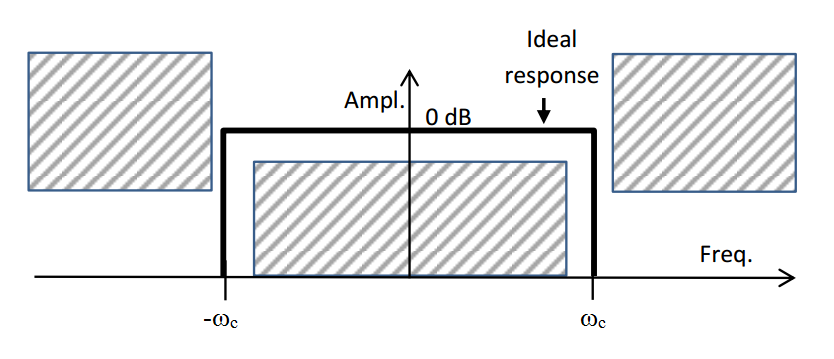
\includegraphics[width=0.6\textwidth]{figures/Ideal_filter.png}
\caption{The ideal frequency response of a lowpass filter.}
\label{fig:IdealFilterApp}
\end{figure}
Which is defined as:
\begin{equation} \label{eq:idealfreq}
H_d(e^{j\omega})=\left\{
\begin{array}{c l}      
    e^{\frac{j\omega M}{2}} & |\omega|\leq\omega_c\\
    0 & \omega_c\leq\pi
\end{array}\right.
\end{equation}
The ideal impulse response can be found by applying the inverse Fourier transformation of \autoref{eq:idealfreq}.
\begin{equation}
h_d[n]=\frac{1}{2\pi}\int_{-\omega_c}^{\omega_c}e^{\frac{j\omega M}{2}} e^{j\omega n} d\omega \Leftrightarrow h_d[n]=\frac{1}{2\pi}\int_{-\omega_c}^{\omega_c}e^{j(n-\frac{M}{2})\omega} d\omega
\end{equation}

By using Eulers rule the expression is reduced to:
\begin{equation}
h_d[n]=\frac{1}{2\pi}\int_{-\omega_c}^{\omega_c}cos\Big((n-\frac{M}{2})\omega\Big)+jsin\Big((n-\frac{M}{2})\omega\Big) d\omega
\end{equation}
\textbf{Explanation} (Sin is an odd function)
\begin{equation}
h_d[n]=\frac{1}{2\pi(n-\frac{M}{2})}\bigg[sin\Big((n-\frac{M}{2})\omega\Big)\bigg]_{-\omega_{c}}^{\omega_{c}}
\end{equation}
where:
\begin{equation}
\int_{a}^{b}cos(ax) dx = \Big[\frac{sin(ax)}{a}\Big]_{a}^{b}
\end{equation}
The integral is expanded:
\begin{equation}
h_d[n]=\frac{1}{2\pi(n-\frac{M}{2})}\bigg[sin\Big(\omega_c(n-\frac{M}{2})\Big)-sin\Big(-\omega_c(n-\frac{M}{2})\Big)\bigg]
\end{equation}
where:
\begin{equation}
sin(-x) = -sin(x)
\end{equation}
Which means that the numenator is doubled equaling:
\begin{equation}
h_d[n]=\frac{sin\Big(\omega_c(n-\frac{M}{2})\Big)}{\pi(n-\frac{M}{2})}\qquad-\infty<n<\infty
\end{equation}
The impulse response is now symmetric around M/2 and the phase is therefore linear. The impulse response is still infinite and non-causal so the impulse response must be truncated.

% Samples the impulse response of an ideal brick-wall filter

\section{Window Method}
The impulse response needs to be truncated. To truncate the impulse response a window function is applied. The most basic window function that can be applied is an rectangular window which basically cuts of the ends of the impulse response. After applying the window function the impulse response can be expressed as:

\begin{equation}
h[n]=h_d[n]\cdot w[n]\qquad\textrm{ where } w[n]\neq0 \textrm{ for } 0<n<M
\end{equation}

An example is shown in \autoref{fig:FIRWindow}, where a Hamming window is applied to the truncated impulse response of a order of 40. The Hamming window prevents the impulse response from stopping abruptly.

\begin{figure}[H]
\centering
\begin{subfigure}[t]{0.45\textwidth}
    \centering
    \tikzsetnextfilename{FIRTruncation}
    % This file was created by matlab2tikz.
%
%The latest updates can be retrieved from
%  http://www.mathworks.com/matlabcentral/fileexchange/22022-matlab2tikz-matlab2tikz
%where you can also make suggestions and rate matlab2tikz.
%
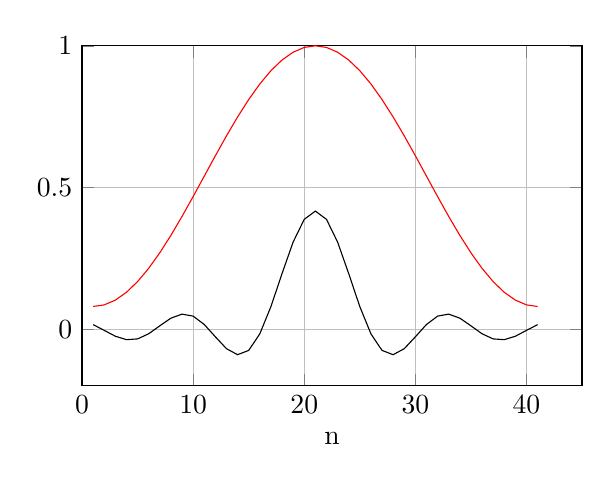
\begin{tikzpicture}

\begin{axis}[%
width=2.5in,
height=1.7in,
at={(1.011in,0.642in)},
scale only axis,
xmin=0,
xmax=45,
xlabel={n},
xmajorgrids,
ymin=-0.2,
ymax=1,
ymajorgrids,
axis background/.style={fill=white}
]
\addplot [color=red,solid,forget plot]
  table[row sep=crcr]{%
1	0.08\\
2	0.0856633633262366\\
3	0.102514002504229\\
4	0.130136998873351\\
5	0.167852182587524\\
6	0.214730880654188\\
7	0.269618783945462\\
8	0.331164370119808\\
9	0.397852182587524\\
10	0.468040146081494\\
11	0.54\\
12	0.611959853918506\\
13	0.682147817412476\\
14	0.748835629880192\\
15	0.810381216054538\\
16	0.865269119345812\\
17	0.912147817412476\\
18	0.949863001126649\\
19	0.977485997495771\\
20	0.994336636673763\\
21	1\\
22	0.994336636673763\\
23	0.977485997495771\\
24	0.949863001126649\\
25	0.912147817412476\\
26	0.865269119345812\\
27	0.810381216054538\\
28	0.748835629880192\\
29	0.682147817412476\\
30	0.611959853918506\\
31	0.54\\
32	0.468040146081494\\
33	0.397852182587524\\
34	0.331164370119808\\
35	0.269618783945462\\
36	0.214730880654188\\
37	0.167852182587524\\
38	0.130136998873351\\
39	0.102514002504229\\
40	0.0856633633262366\\
41	0.08\\
};
\addplot [color=black,solid,forget plot]
  table[row sep=crcr]{%
1	0.0159154943091895\\
2	-0.00437345025153354\\
3	-0.0250087865599196\\
4	-0.0371278471742826\\
5	-0.034458055963862\\
6	-0.0162415893067405\\
7	0.0117692372555402\\
8	0.0388511094540975\\
9	0.0530516476972984\\
10	0.0459149475366605\\
11	0.0164769321577561\\
12	-0.0270693155112343\\
13	-0.068916111927724\\
14	-0.0901676288518291\\
15	-0.0750263596797588\\
16	-0.0166191109558273\\
17	0.0795774715459477\\
18	0.196053325894134\\
19	0.307463739828057\\
20	0.387549562361695\\
21	0.416666666666667\\
22	0.387549562361695\\
23	0.307463739828057\\
24	0.196053325894134\\
25	0.0795774715459477\\
26	-0.0166191109558273\\
27	-0.0750263596797588\\
28	-0.0901676288518291\\
29	-0.068916111927724\\
30	-0.0270693155112343\\
31	0.0164769321577561\\
32	0.0459149475366605\\
33	0.0530516476972984\\
34	0.0388511094540975\\
35	0.0117692372555402\\
36	-0.0162415893067405\\
37	-0.034458055963862\\
38	-0.0371278471742826\\
39	-0.0250087865599196\\
40	-0.00437345025153354\\
41	0.0159154943091895\\
};
\end{axis}
\end{tikzpicture}%
    \caption{Hamming window is applied to the truncated impulse response.}
    \label{fig:FIRTruncation}
\end{subfigure}
\begin{subfigure}[t]{0.45\textwidth}
    \centering
    \tikzsetnextfilename{FIRHamming}
    % This file was created by matlab2tikz.
%
%The latest updates can be retrieved from
%  http://www.mathworks.com/matlabcentral/fileexchange/22022-matlab2tikz-matlab2tikz
%where you can also make suggestions and rate matlab2tikz.
%
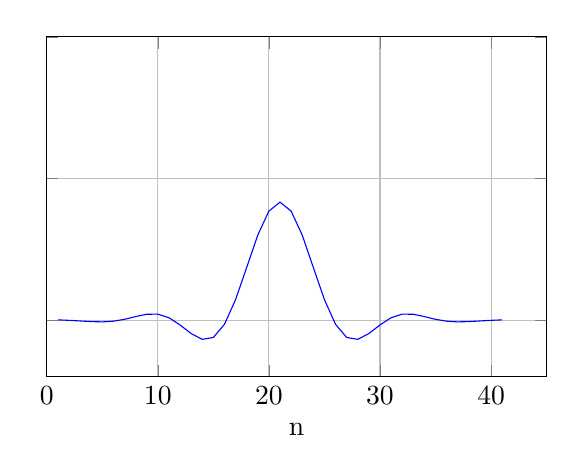
\begin{tikzpicture}

\begin{axis}[%
width=2.5in,
height=1.7in,
at={(1.011in,0.642in)},
scale only axis,
xmin=0,
xmax=45,
xlabel={n},
xmajorgrids,
ymin=-0.2,
ymax=1,
yticklabels={\empty},
ymajorgrids,
axis background/.style={fill=white}
]
\addplot [color=blue,solid,forget plot]
  table[row sep=crcr]{%
1	0.00127323954473516\\
2	-0.000374644457886338\\
3	-0.00256375080803134\\
4	-0.00483170660588955\\
5	-0.00578385990125729\\
6	-0.00348757077506003\\
7	0.00317320743680438\\
8	0.0128661031908219\\
9	0.0211067138262346\\
10	0.0214900387523827\\
11	0.00889754336518831\\
12	-0.0165653343659289\\
13	-0.0470109753360508\\
14	-0.0675207331460627\\
15	-0.0607999525934281\\
16	-0.014380003501059\\
17	0.0725864169858396\\
18	0.186223800514663\\
19	0.300541500419609\\
20	0.385354728383117\\
21	0.416666666666667\\
22	0.385354728383117\\
23	0.300541500419609\\
24	0.186223800514663\\
25	0.0725864169858396\\
26	-0.014380003501059\\
27	-0.0607999525934281\\
28	-0.0675207331460627\\
29	-0.0470109753360508\\
30	-0.0165653343659289\\
31	0.00889754336518831\\
32	0.0214900387523827\\
33	0.0211067138262346\\
34	0.0128661031908219\\
35	0.00317320743680438\\
36	-0.00348757077506003\\
37	-0.00578385990125729\\
38	-0.00483170660588955\\
39	-0.00256375080803134\\
40	-0.000374644457886338\\
41	0.00127323954473516\\
};
\end{axis}
\end{tikzpicture}%
    \caption{Impulse response after applying Hamming window.}
    \label{fig:FIRHamming}
\end{subfigure}
\caption{Applying a Hamming window to a truncated impulse response.}
\label{fig:FIRWindow}
\end{figure} 

If no window function is applied the truncated impulse response, the window function is per default a rectangular window. The rectangular window attenuates fast as the main lope but the attenuation at the first side is not high. Applying the Hamming window reduces the steepness but the attenuation at the first side lope is bigger. Also the pass-band ripple is reduced. This is illustrated in \autoref{fig:FIRFrequencyResp}.

\begin{figure}[H]
    \centering
    \tikzsetnextfilename{FIRFrequencyResp}
    % This file was created by matlab2tikz.
%
%The latest updates can be retrieved from
%  http://www.mathworks.com/matlabcentral/fileexchange/22022-matlab2tikz-matlab2tikz
%where you can also make suggestions and rate matlab2tikz.
%
\begin{tikzpicture}

\begin{axis}[%
width=4in,
height=3in,
at={(1.011in,0.642in)},
scale only axis,
xmin=0,
xmax=12000,
xlabel={Frequency [Hz]},
xmajorgrids,
ymin=-140,
ymax=20,
ylabel={Magnitude [dB]},
ymajorgrids,
axis background/.style={fill=white}
]
\addplot [color=blue,solid]
  table[row sep=crcr]{%
0.159154943091895	6.00780568530664\\
1.35920698794698	6.00780576338686\\
2.55925903280207	6.00780596488919\\
3.75931107765716	6.0078062898114\\
4.95936312251225	6.00780673814993\\
6.15941516736734	6.00780730989984\\
7.35946721222242	6.00780800505487\\
8.55951925707751	6.00780882360735\\
9.7595713019326	6.00780976554833\\
10.9596233467877	6.0078108308674\\
12.1596753916428	6.00781201955291\\
13.3597274364979	6.00781333159177\\
14.559779481353	6.00781476696959\\
15.759831526208	6.00781632567056\\
16.9598835710631	6.00781800767759\\
18.1599356159182	6.00781981297219\\
19.3599876607733	6.00782174153452\\
20.5600397056284	6.00782379334337\\
21.7600917504835	6.00782596837624\\
22.9601437953386	6.00782826660919\\
24.1601958401937	6.00783068801701\\
25.3602478850487	6.00783323257308\\
26.5602999299038	6.00783590024941\\
27.7603519747589	6.00783869101674\\
28.960404019614	6.00784160484436\\
30.1604560644691	6.0078446417003\\
31.3605081093242	6.00784780155116\\
32.5605601541793	6.00785108436225\\
33.7606121990344	6.00785449009748\\
34.9606642438895	6.00785801871942\\
36.1607162887445	6.00786167018934\\
37.3607683335996	6.00786544446708\\
38.5608203784547	6.0078693415112\\
39.7608724233098	6.00787336127886\\
40.9609244681649	6.0078775037259\\
42.16097651302	6.00788176880682\\
43.3610285578751	6.00788615647475\\
44.5610806027302	6.00789066668148\\
45.7611326475852	6.00789529937747\\
46.9611846924403	6.0079000545118\\
48.1612367372954	6.00790493203223\\
49.3612887821505	6.00790993188516\\
50.5613408270056	6.00791505401568\\
51.7613928718607	6.00792029836751\\
52.9614449167158	6.00792566488302\\
54.1614969615709	6.00793115350325\\
55.361549006426	6.00793676416789\\
56.561601051281	6.00794249681531\\
57.7616530961361	6.00794835138252\\
58.9617051409912	6.00795432780519\\
60.1617571858463	6.00796042601764\\
61.3618092307014	6.00796664595292\\
62.5618612755565	6.00797298754264\\
63.7619133204116	6.00797945071716\\
64.9619653652667	6.00798603540544\\
66.1620174101217	6.00799274153516\\
67.3620694549768	6.00799956903262\\
68.5621214998319	6.00800651782281\\
69.762173544687	6.00801358782941\\
70.9622255895421	6.00802077897471\\
72.1622776343972	6.00802809117972\\
73.3623296792523	6.0080355243641\\
74.5623817241074	6.00804307844617\\
75.7624337689625	6.00805075334295\\
76.9624858138175	6.00805854897011\\
78.1625378586726	6.00806646524202\\
79.3625899035277	6.00807450207165\\
80.5626419483828	6.00808265937077\\
81.7626939932379	6.00809093704971\\
82.962746038093	6.00809933501756\\
84.1627980829481	6.00810785318202\\
85.3628501278032	6.00811649144952\\
86.5629021726582	6.00812524972516\\
87.7629542175133	6.00813412791271\\
88.9630062623684	6.00814312591463\\
90.1630583072235	6.00815224363205\\
91.3631103520786	6.00816148096481\\
92.5631623969337	6.00817083781141\\
93.7632144417888	6.0081803140691\\
94.9632664866439	6.00818990963369\\
96.163318531499	6.00819962439982\\
97.363370576354	6.00820945826071\\
98.5634226212091	6.00821941110837\\
99.7634746660642	6.00822948283343\\
100.963526710919	6.00823967332523\\
102.163578755774	6.00824998247181\\
103.363630800629	6.00826041015992\\
104.563682845485	6.00827095627499\\
105.76373489034	6.00828162070118\\
106.963786935195	6.00829240332131\\
108.16383898005	6.00830330401691\\
109.363891024905	6.00831432266824\\
110.56394306976	6.00832545915422\\
111.763995114615	6.00833671335254\\
112.96404715947	6.00834808513952\\
114.164099204325	6.00835957439025\\
115.36415124918	6.00837118097851\\
116.564203294035	6.00838290477676\\
117.764255338891	6.00839474565624\\
118.964307383746	6.00840670348684\\
120.164359428601	6.00841877813721\\
121.364411473456	6.00843096947466\\
122.564463518311	6.00844327736529\\
123.764515563166	6.00845570167387\\
124.964567608021	6.00846824226391\\
126.164619652876	6.00848089899765\\
127.364671697731	6.00849367173603\\
128.564723742586	6.00850656033873\\
129.764775787441	6.00851956466419\\
130.964827832296	6.00853268456952\\
132.164879877152	6.00854591991057\\
133.364931922007	6.00855927054196\\
134.564983966862	6.00857273631703\\
135.765036011717	6.00858631708785\\
136.965088056572	6.00860001270522\\
138.165140101427	6.00861382301868\\
139.365192146282	6.00862774787651\\
140.565244191137	6.00864178712575\\
141.765296235992	6.00865594061218\\
142.965348280847	6.0086702081803\\
144.165400325702	6.0086845896734\\
145.365452370558	6.00869908493345\\
146.565504415413	6.00871369380124\\
147.765556460268	6.0087284161163\\
148.965608505123	6.00874325171688\\
150.165660549978	6.00875820044\\
151.365712594833	6.00877326212149\\
152.565764639688	6.00878843659583\\
153.765816684543	6.00880372369639\\
154.965868729398	6.00881912325519\\
156.165920774253	6.00883463510309\\
157.365972819108	6.00885025906968\\
158.566024863964	6.00886599498333\\
159.766076908819	6.00888184267121\\
160.966128953674	6.0088978019592\\
162.166180998529	6.00891387267201\\
163.366233043384	6.0089300546331\\
164.566285088239	6.00894634766471\\
165.766337133094	6.00896275158786\\
166.966389177949	6.00897926622238\\
168.166441222804	6.00899589138685\\
169.366493267659	6.00901262689866\\
170.566545312514	6.00902947257396\\
171.76659735737	6.00904642822772\\
172.966649402225	6.00906349367367\\
174.16670144708	6.00908066872439\\
175.366753491935	6.00909795319122\\
176.56680553679	6.00911534688426\\
177.766857581645	6.00913284961251\\
178.9669096265	6.00915046118368\\
180.166961671355	6.00916818140433\\
181.36701371621	6.00918601007984\\
182.567065761065	6.00920394701434\\
183.76711780592	6.00922199201083\\
184.967169850775	6.00924014487112\\
186.167221895631	6.0092584053958\\
187.367273940486	6.0092767733843\\
188.567325985341	6.0092952486349\\
189.767378030196	6.00931383094463\\
190.967430075051	6.00933252010942\\
192.167482119906	6.00935131592398\\
193.367534164761	6.00937021818186\\
194.567586209616	6.00938922667548\\
195.767638254471	6.00940834119601\\
196.967690299326	6.00942756153356\\
198.167742344181	6.00944688747698\\
199.367794389037	6.00946631881404\\
200.567846433892	6.00948585533134\\
201.767898478747	6.00950549681425\\
202.967950523602	6.00952524304709\\
204.168002568457	6.00954509381298\\
205.368054613312	6.0095650488939\\
206.568106658167	6.00958510807067\\
207.768158703022	6.00960527112299\\
208.968210747877	6.00962553782944\\
210.168262792732	6.00964590796742\\
211.368314837587	6.00966638131321\\
212.568366882443	6.00968695764196\\
213.768418927298	6.00970763672769\\
214.968470972153	6.00972841834331\\
216.168523017008	6.00974930226057\\
217.368575061863	6.00977028825012\\
218.568627106718	6.00979137608151\\
219.768679151573	6.00981256552313\\
220.968731196428	6.0098338563423\\
222.168783241283	6.00985524830519\\
223.368835286138	6.00987674117686\\
224.568887330993	6.0098983347213\\
225.768939375848	6.0099200287014\\
226.968991420704	6.00994182287887\\
228.169043465559	6.0099637170144\\
229.369095510414	6.00998571086759\\
230.569147555269	6.01000780419687\\
231.769199600124	6.01002999675967\\
232.969251644979	6.01005228831226\\
234.169303689834	6.01007467860986\\
235.369355734689	6.0100971674066\\
236.569407779544	6.01011975445553\\
237.769459824399	6.01014243950863\\
238.969511869254	6.01016522231681\\
240.16956391411	6.01018810262989\\
241.369615958965	6.01021108019664\\
242.56966800382	6.01023415476473\\
243.769720048675	6.01025732608079\\
244.96977209353	6.01028059389042\\
246.169824138385	6.01030395793814\\
247.36987618324	6.01032741796737\\
248.569928228095	6.01035097372054\\
249.76998027295	6.01037462493902\\
250.970032317805	6.01039837136311\\
252.17008436266	6.01042221273207\\
253.370136407516	6.01044614878418\\
254.570188452371	6.01047017925656\\
255.770240497226	6.01049430388542\\
256.970292542081	6.01051852240587\\
258.170344586936	6.01054283455202\\
259.370396631791	6.01056724005693\\
260.570448676646	6.01059173865267\\
261.770500721501	6.01061633007025\\
262.970552766356	6.0106410140397\\
264.170604811211	6.01066579029003\\
265.370656856066	6.0106906585492\\
266.570708900921	6.01071561854423\\
267.770760945777	6.01074067000109\\
268.970812990632	6.01076581264476\\
270.170865035487	6.01079104619922\\
271.370917080342	6.01081637038745\\
272.570969125197	6.01084178493145\\
273.771021170052	6.01086728955221\\
274.971073214907	6.01089288396978\\
276.171125259762	6.01091856790319\\
277.371177304617	6.01094434107048\\
278.571229349472	6.01097020318874\\
279.771281394327	6.01099615397406\\
280.971333439183	6.01102219314162\\
282.171385484038	6.01104832040555\\
283.371437528893	6.01107453547909\\
284.571489573748	6.01110083807446\\
285.771541618603	6.01112722790295\\
286.971593663458	6.01115370467492\\
288.171645708313	6.01118026809974\\
289.371697753168	6.01120691788586\\
290.571749798023	6.01123365374076\\
291.771801842878	6.01126047537099\\
292.971853887733	6.01128738248219\\
294.171905932589	6.011314374779\\
295.371957977444	6.0113414519652\\
296.572010022299	6.01136861374359\\
297.772062067154	6.0113958598161\\
298.972114112009	6.01142318988368\\
300.172166156864	6.0114506036464\\
301.372218201719	6.0114781008034\\
302.572270246574	6.0115056810529\\
303.772322291429	6.01153334409224\\
304.972374336284	6.01156108961784\\
306.172426381139	6.01158891732522\\
307.372478425994	6.01161682690902\\
308.57253047085	6.01164481806292\\
309.772582515705	6.01167289047981\\
310.97263456056	6.01170104385161\\
312.172686605415	6.01172927786939\\
313.37273865027	6.01175759222336\\
314.572790695125	6.01178598660281\\
315.77284273998	6.01181446069616\\
316.972894784835	6.01184301419104\\
318.17294682969	6.01187164677409\\
319.372998874545	6.01190035813115\\
320.5730509194	6.01192914794724\\
321.773102964255	6.01195801590646\\
322.973155009111	6.01198696169208\\
324.173207053966	6.01201598498651\\
325.373259098821	6.01204508547135\\
326.573311143676	6.01207426282734\\
327.773363188531	6.01210351673437\\
328.973415233386	6.01213284687147\\
330.173467278241	6.01216225291692\\
331.373519323096	6.01219173454811\\
332.573571367951	6.01222129144162\\
333.773623412806	6.01225092327321\\
334.973675457661	6.01228062971783\\
336.173727502517	6.01231041044962\\
337.373779547372	6.01234026514191\\
338.573831592227	6.0123701934672\\
339.773883637082	6.01240019509722\\
340.973935681937	6.01243026970288\\
342.173987726792	6.01246041695433\\
343.374039771647	6.01249063652088\\
344.574091816502	6.01252092807111\\
345.774143861357	6.01255129127275\\
346.974195906212	6.0125817257928\\
348.174247951067	6.01261223129751\\
349.374299995923	6.01264280745225\\
350.574352040778	6.01267345392174\\
351.774404085633	6.0127041703699\\
352.974456130488	6.01273495645983\\
354.174508175343	6.01276581185395\\
355.374560220198	6.01279673621389\\
356.574612265053	6.01282772920054\\
357.774664309908	6.01285879047405\\
358.974716354763	6.01288991969383\\
360.174768399618	6.01292111651851\\
361.374820444473	6.01295238060606\\
362.574872489328	6.01298371161366\\
363.774924534184	6.01301510919781\\
364.974976579039	6.01304657301422\\
366.175028623894	6.01307810271795\\
367.375080668749	6.01310969796335\\
368.575132713604	6.01314135840399\\
369.775184758459	6.01317308369278\\
370.975236803314	6.01320487348192\\
372.175288848169	6.01323672742294\\
373.375340893024	6.01326864516662\\
374.575392937879	6.01330062636307\\
375.775444982735	6.01333267066177\\
376.97549702759	6.0133647777114\\
378.175549072445	6.01339694716009\\
379.3756011173	6.01342917865518\\
380.575653162155	6.01346147184344\\
381.77570520701	6.0134938263709\\
382.975757251865	6.01352624188295\\
384.17580929672	6.01355871802436\\
385.375861341575	6.01359125443917\\
386.57591338643	6.01362385077079\\
387.775965431285	6.01365650666207\\
388.97601747614	6.01368922175509\\
390.176069520996	6.01372199569137\\
391.376121565851	6.01375482811177\\
392.576173610706	6.01378771865654\\
393.776225655561	6.01382066696527\\
394.976277700416	6.01385367267695\\
396.176329745271	6.01388673542996\\
397.376381790126	6.01391985486204\\
398.576433834981	6.01395303061031\\
399.776485879836	6.01398626231135\\
400.976537924691	6.01401954960107\\
402.176589969546	6.01405289211481\\
403.376642014402	6.0140862894873\\
404.576694059257	6.0141197413527\\
405.776746104112	6.01415324734461\\
406.976798148967	6.01418680709596\\
408.176850193822	6.0142204202392\\
409.376902238677	6.01425408640614\\
410.576954283532	6.01428780522807\\
411.777006328387	6.01432157633568\\
412.977058373242	6.01435539935914\\
414.177110418097	6.01438927392798\\
415.377162462952	6.01442319967128\\
416.577214507807	6.01445717621749\\
417.777266552663	6.01449120319459\\
418.977318597518	6.01452528022997\\
420.177370642373	6.01455940695049\\
421.377422687228	6.01459358298249\\
422.577474732083	6.01462780795178\\
423.777526776938	6.01466208148366\\
424.977578821793	6.01469640320289\\
426.177630866648	6.01473077273372\\
427.377682911503	6.0147651896999\\
428.577734956358	6.01479965372469\\
429.777787001213	6.0148341644308\\
430.977839046069	6.01486872144051\\
432.177891090924	6.01490332437554\\
433.377943135779	6.01493797285717\\
434.577995180634	6.01497266650617\\
435.778047225489	6.01500740494283\\
436.978099270344	6.01504218778702\\
438.178151315199	6.01507701465804\\
439.378203360054	6.0151118851748\\
440.578255404909	6.01514679895574\\
441.778307449764	6.0151817556188\\
442.978359494619	6.01521675478152\\
444.178411539474	6.01525179606093\\
445.37846358433	6.01528687907371\\
446.578515629185	6.01532200343596\\
447.77856767404	6.01535716876351\\
448.978619718895	6.01539237467161\\
450.17867176375	6.01542762077516\\
451.378723808605	6.01546290668865\\
452.57877585346	6.01549823202609\\
453.778827898315	6.01553359640111\\
454.97887994317	6.01556899942698\\
456.178931988025	6.01560444071645\\
457.37898403288	6.01563991988198\\
458.579036077736	6.01567543653558\\
459.779088122591	6.01571099028888\\
460.979140167446	6.01574658075311\\
462.179192212301	6.01578220753912\\
463.379244257156	6.0158178702574\\
464.579296302011	6.01585356851806\\
465.779348346866	6.01588930193082\\
466.979400391721	6.01592507010507\\
468.179452436576	6.01596087264981\\
469.379504481431	6.01599670917369\\
470.579556526286	6.016032579285\\
471.779608571142	6.01606848259173\\
472.979660615997	6.01610441870147\\
474.179712660852	6.01614038722147\\
475.379764705707	6.01617638775872\\
476.579816750562	6.01621241991979\\
477.779868795417	6.016248483311\\
478.979920840272	6.01628457753828\\
480.179972885127	6.01632070220732\\
481.380024929982	6.01635685692344\\
482.580076974837	6.01639304129166\\
483.780129019692	6.01642925491674\\
484.980181064547	6.01646549740309\\
486.180233109403	6.01650176835487\\
487.380285154258	6.01653806737593\\
488.580337199113	6.01657439406984\\
489.780389243968	6.01661074803986\\
490.980441288823	6.01664712888905\\
492.180493333678	6.01668353622013\\
493.380545378533	6.01671996963558\\
494.580597423388	6.01675642873765\\
495.780649468243	6.01679291312827\\
496.980701513098	6.01682942240916\\
498.180753557953	6.01686595618179\\
499.380805602809	6.01690251404737\\
500.580857647664	6.01693909560687\\
501.780909692519	6.01697570046109\\
502.980961737374	6.01701232821052\\
504.181013782229	6.01704897845546\\
505.381065827084	6.01708565079598\\
506.581117871939	6.01712234483197\\
507.781169916794	6.01715906016306\\
508.981221961649	6.01719579638868\\
510.181274006504	6.01723255310812\\
511.381326051359	6.0172693299204\\
512.581378096215	6.0173061264244\\
513.78143014107	6.01734294221878\\
514.981482185925	6.01737977690204\\
516.18153423078	6.01741663007246\\
517.381586275635	6.01745350132819\\
518.58163832049	6.01749039026722\\
519.781690365345	6.01752729648734\\
520.9817424102	6.01756421958622\\
522.181794455055	6.01760115916132\\
523.38184649991	6.01763811480999\\
524.581898544765	6.01767508612943\\
525.781950589621	6.01771207271671\\
526.982002634476	6.01774907416872\\
528.182054679331	6.0177860900823\\
529.382106724186	6.01782312005404\\
530.582158769041	6.01786016368056\\
531.782210813896	6.01789722055824\\
532.982262858751	6.01793429028339\\
534.182314903606	6.01797137245224\\
535.382366948461	6.01800846666085\\
536.582418993316	6.01804557250528\\
537.782471038171	6.01808268958139\\
538.982523083027	6.01811981748502\\
540.182575127882	6.01815695581191\\
541.382627172737	6.01819410415771\\
542.582679217592	6.01823126211801\\
543.782731262447	6.01826842928831\\
544.982783307302	6.01830560526405\\
546.182835352157	6.01834278964065\\
547.382887397012	6.0183799820134\\
548.582939441867	6.01841718197763\\
549.782991486722	6.01845438912852\\
550.983043531577	6.01849160306127\\
552.183095576432	6.01852882337106\\
553.383147621288	6.01856604965299\\
554.583199666143	6.01860328150216\\
555.783251710998	6.01864051851363\\
556.983303755853	6.01867776028249\\
558.183355800708	6.01871500640373\\
559.383407845563	6.01875225647241\\
560.583459890418	6.01878951008356\\
561.783511935273	6.01882676683217\\
562.983563980128	6.01886402631333\\
564.183616024983	6.01890128812205\\
565.383668069838	6.01893855185339\\
566.583720114694	6.01897581710244\\
567.783772159549	6.0190130834643\\
568.983824204404	6.0190503505341\\
570.183876249259	6.01908761790699\\
571.383928294114	6.0191248851782\\
572.583980338969	6.01916215194299\\
573.784032383824	6.01919941779661\\
574.984084428679	6.01923668233447\\
576.184136473534	6.01927394515193\\
577.384188518389	6.01931120584449\\
578.584240563244	6.01934846400766\\
579.784292608099	6.01938571923709\\
580.984344652955	6.01942297112843\\
582.18439669781	6.01946021927749\\
583.384448742665	6.01949746328007\\
584.58450078752	6.01953470273216\\
585.784552832375	6.0195719372298\\
586.98460487723	6.01960916636913\\
588.184656922085	6.01964638974639\\
589.38470896694	6.01968360695793\\
590.584761011795	6.01972081760026\\
591.78481305665	6.01975802126994\\
592.984865101505	6.01979521756371\\
594.18491714636	6.0198324060784\\
595.384969191216	6.01986958641099\\
596.585021236071	6.01990675815862\\
597.785073280926	6.01994392091855\\
598.985125325781	6.01998107428819\\
600.185177370636	6.02001821786511\\
601.385229415491	6.02005535124703\\
602.585281460346	6.02009247403182\\
603.785333505201	6.02012958581757\\
604.985385550056	6.02016668620247\\
606.185437594911	6.02020377478494\\
607.385489639767	6.02024085116357\\
608.585541684621	6.02027791493713\\
609.785593729477	6.02031496570458\\
610.985645774332	6.02035200306507\\
612.185697819187	6.02038902661796\\
613.385749864042	6.02042603596284\\
614.585801908897	6.02046303069945\\
615.785853953752	6.02050001042782\\
616.985905998607	6.02053697474814\\
618.185958043462	6.02057392326082\\
619.386010088317	6.02061085556657\\
620.586062133173	6.02064777126626\\
621.786114178028	6.02068466996104\\
622.986166222883	6.0207215512523\\
624.186218267738	6.02075841474163\\
625.386270312593	6.02079526003095\\
626.586322357448	6.02083208672242\\
627.786374402303	6.02086889441838\\
628.986426447158	6.02090568272155\\
630.186478492013	6.02094245123486\\
631.386530536868	6.02097919956151\\
632.586582581723	6.02101592730504\\
633.786634626578	6.02105263406923\\
634.986686671434	6.02108931945812\\
636.186738716289	6.02112598307615\\
637.386790761144	6.02116262452794\\
638.586842805999	6.02119924341851\\
639.786894850854	6.02123583935312\\
640.986946895709	6.02127241193741\\
642.186998940564	6.02130896077727\\
643.387050985419	6.02134548547898\\
644.587103030274	6.02138198564911\\
645.787155075129	6.02141846089457\\
646.987207119984	6.02145491082262\\
648.187259164839	6.02149133504085\\
649.387311209695	6.02152773315723\\
650.58736325455	6.02156410478001\\
651.787415299405	6.02160044951787\\
652.98746734426	6.02163676697983\\
654.187519389115	6.02167305677528\\
655.38757143397	6.02170931851395\\
656.587623478825	6.02174555180599\\
657.78767552368	6.02178175626191\\
658.987727568535	6.02181793149262\\
660.18777961339	6.02185407710938\\
661.387831658245	6.0218901927239\\
662.587883703101	6.02192627794824\\
663.787935747956	6.02196233239493\\
664.987987792811	6.02199835567682\\
666.188039837666	6.02203434740725\\
667.388091882521	6.02207030719994\\
668.588143927376	6.02210623466907\\
669.788195972231	6.0221421294292\\
670.988248017086	6.02217799109535\\
672.188300061941	6.02221381928296\\
673.388352106796	6.02224961360796\\
674.588404151651	6.02228537368665\\
675.788456196507	6.02232109913584\\
676.988508241362	6.0223567895728\\
678.188560286217	6.02239244461521\\
679.388612331072	6.02242806388125\\
680.588664375927	6.0224636469896\\
681.788716420782	6.02249919355934\\
682.988768465637	6.02253470321009\\
684.188820510492	6.02257017556195\\
685.388872555347	6.02260561023545\\
686.588924600202	6.02264100685169\\
687.788976645057	6.02267636503224\\
688.989028689913	6.02271168439914\\
690.189080734767	6.02274696457498\\
691.389132779623	6.02278220518285\\
692.589184824478	6.02281740584637\\
693.789236869333	6.02285256618962\\
694.989288914188	6.02288768583728\\
696.189340959043	6.02292276441454\\
697.389393003898	6.0229578015471\\
698.589445048753	6.02299279686123\\
699.789497093608	6.0230277499837\\
700.989549138463	6.02306266054189\\
702.189601183318	6.02309752816371\\
703.389653228174	6.02313235247757\\
704.589705273029	6.02316713311255\\
705.789757317884	6.02320186969822\\
706.989809362739	6.02323656186472\\
708.189861407594	6.02327120924282\\
709.389913452449	6.02330581146384\\
710.589965497304	6.02334036815965\\
711.790017542159	6.0233748789628\\
712.990069587014	6.02340934350633\\
714.190121631869	6.02344376142395\\
715.390173676724	6.02347813234995\\
716.59022572158	6.02351245591924\\
717.790277766435	6.02354673176733\\
718.99032981129	6.02358095953036\\
720.190381856145	6.02361513884506\\
721.390433901	6.02364926934882\\
722.590485945855	6.02368335067967\\
723.79053799071	6.02371738247625\\
724.990590035565	6.02375136437781\\
726.19064208042	6.02378529602432\\
727.390694125275	6.02381917705635\\
728.59074617013	6.02385300711514\\
729.790798214986	6.02388678584256\\
730.990850259841	6.02392051288119\\
732.190902304696	6.02395418787423\\
733.390954349551	6.02398781046558\\
734.591006394406	6.02402138029981\\
735.791058439261	6.02405489702217\\
736.991110484116	6.02408836027858\\
738.191162528971	6.02412176971568\\
739.391214573826	6.02415512498077\\
740.591266618681	6.02418842572187\\
741.791318663536	6.02422167158771\\
742.991370708391	6.02425486222771\\
744.191422753246	6.02428799729199\\
745.391474798102	6.0243210764314\\
746.591526842957	6.02435409929751\\
747.791578887812	6.02438706554264\\
748.991630932667	6.02441997481981\\
750.191682977522	6.02445282678276\\
751.391735022377	6.02448562108599\\
752.591787067232	6.02451835738475\\
753.791839112087	6.024551035335\\
754.991891156942	6.02458365459353\\
756.191943201797	6.02461621481775\\
757.391995246653	6.02464871566599\\
758.592047291508	6.02468115679723\\
759.792099336363	6.02471353787124\\
760.992151381218	6.02474585854861\\
762.192203426073	6.02477811849064\\
763.392255470928	6.02481031735945\\
764.592307515783	6.02484245481795\\
765.792359560638	6.02487453052984\\
766.992411605493	6.02490654415959\\
768.192463650348	6.02493849537249\\
769.392515695203	6.02497038383462\\
770.592567740058	6.02500220921287\\
771.792619784914	6.02503397117496\\
772.992671829769	6.02506566938938\\
774.192723874624	6.02509730352553\\
775.392775919479	6.0251288732535\\
776.592827964334	6.02516037824432\\
777.792880009189	6.02519181816984\\
778.992932054044	6.02522319270265\\
780.192984098899	6.02525450151635\\
781.393036143754	6.02528574428523\\
782.593088188609	6.02531692068448\\
783.793140233464	6.02534803039018\\
784.99319227832	6.02537907307924\\
786.193244323175	6.02541004842942\\
787.39329636803	6.02544095611938\\
788.593348412885	6.0254717958286\\
789.79340045774	6.0255025672375\\
790.993452502595	6.02553327002731\\
792.19350454745	6.02556390388021\\
793.393556592305	6.02559446847921\\
794.59360863716	6.02562496350824\\
795.793660682015	6.02565538865212\\
796.99371272687	6.02568574359661\\
798.193764771726	6.02571602802827\\
799.393816816581	6.02574624163468\\
800.593868861436	6.02577638410425\\
801.793920906291	6.02580645512638\\
802.993972951146	6.02583645439131\\
804.194024996001	6.02586638159029\\
805.394077040856	6.0258962364154\\
806.594129085711	6.02592601855977\\
807.794181130566	6.02595572771733\\
808.994233175421	6.02598536358308\\
810.194285220276	6.02601492585289\\
811.394337265132	6.02604441422359\\
812.594389309987	6.02607382839297\\
813.794441354842	6.02610316805977\\
814.994493399697	6.0261324329237\\
816.194545444552	6.02616162268544\\
817.394597489407	6.02619073704661\\
818.594649534262	6.02621977570982\\
819.794701579117	6.02624873837869\\
820.994753623972	6.02627762475775\\
822.194805668827	6.02630643455255\\
823.394857713682	6.02633516746968\\
824.594909758537	6.02636382321662\\
825.794961803392	6.0263924015019\\
826.995013848248	6.02642090203511\\
828.195065893103	6.0264493245267\\
829.395117937958	6.02647766868826\\
830.595169982813	6.02650593423234\\
831.795222027668	6.0265341208725\\
832.995274072523	6.02656222832333\\
834.195326117378	6.02659025630043\\
835.395378162233	6.02661820452046\\
836.595430207088	6.02664607270107\\
837.795482251944	6.02667386056096\\
838.995534296798	6.0267015678199\\
840.195586341654	6.02672919419866\\
841.395638386509	6.02675673941907\\
842.595690431364	6.026784203204\\
843.795742476219	6.0268115852774\\
844.995794521074	6.02683888536427\\
846.195846565929	6.02686610319065\\
847.395898610784	6.02689323848368\\
848.595950655639	6.02692029097154\\
849.796002700494	6.02694726038348\\
850.996054745349	6.02697414644983\\
852.196106790204	6.02700094890204\\
853.39615883506	6.02702766747259\\
854.596210879915	6.02705430189509\\
855.79626292477	6.0270808519042\\
856.996314969625	6.0271073172357\\
858.19636701448	6.02713369762648\\
859.396419059335	6.02715999281448\\
860.59647110419	6.02718620253883\\
861.796523149045	6.02721232653969\\
862.9965751939	6.02723836455837\\
864.196627238755	6.02726431633729\\
865.39667928361	6.02729018162001\\
866.596731328466	6.02731596015117\\
867.796783373321	6.02734165167658\\
868.996835418176	6.02736725594316\\
870.196887463031	6.02739277269898\\
871.396939507886	6.02741820169322\\
872.596991552741	6.02744354267623\\
873.797043597596	6.0274687953995\\
874.997095642451	6.02749395961563\\
876.197147687306	6.02751903507844\\
877.397199732161	6.02754402154288\\
878.597251777016	6.02756891876501\\
879.797303821872	6.02759372650213\\
880.997355866726	6.02761844451264\\
882.197407911582	6.02764307255616\\
883.397459956437	6.02766761039346\\
884.597512001292	6.02769205778648\\
885.797564046147	6.02771641449835\\
886.997616091002	6.0277406802934\\
888.197668135857	6.0277648549371\\
889.397720180712	6.02778893819615\\
890.597772225567	6.02781292983845\\
891.797824270422	6.02783682963305\\
892.997876315277	6.02786063735025\\
894.197928360133	6.02788435276154\\
895.397980404988	6.02790797563958\\
896.598032449843	6.02793150575831\\
897.798084494698	6.02795494289283\\
898.998136539553	6.02797828681945\\
900.198188584408	6.02800153731575\\
901.398240629263	6.02802469416045\\
902.598292674118	6.02804775713364\\
903.798344718973	6.02807072601648\\
904.998396763828	6.02809360059146\\
906.198448808683	6.02811638064227\\
907.398500853538	6.02813906595388\\
908.598552898394	6.02816165631244\\
909.798604943249	6.02818415150538\\
910.998656988104	6.02820655132141\\
912.198709032959	6.02822885555041\\
913.398761077814	6.02825106398361\\
914.598813122669	6.02827317641345\\
915.798865167524	6.02829519263361\\
916.998917212379	6.02831711243908\\
918.198969257234	6.02833893562609\\
919.399021302089	6.02836066199217\\
920.599073346944	6.02838229133608\\
921.7991253918	6.02840382345789\\
922.999177436655	6.02842525815896\\
924.19922948151	6.02844659524188\\
925.399281526365	6.02846783451059\\
926.59933357122	6.02848897577029\\
927.799385616075	6.02851001882744\\
928.99943766093	6.02853096348986\\
930.199489705785	6.02855180956665\\
931.39954175064	6.02857255686816\\
932.599593795495	6.02859320520613\\
933.79964584035	6.0286137543935\\
934.999697885206	6.02863420424461\\
936.199749930061	6.02865455457509\\
937.399801974916	6.02867480520187\\
938.599854019771	6.02869495594322\\
939.799906064626	6.0287150066187\\
940.999958109481	6.02873495704923\\
942.200010154336	6.02875480705703\\
943.400062199191	6.02877455646567\\
944.600114244046	6.02879420510003\\
945.800166288901	6.02881375278635\\
947.000218333756	6.02883319935221\\
948.200270378612	6.02885254462651\\
949.400322423467	6.02887178843952\\
950.600374468322	6.0288909306228\\
951.800426513177	6.02890997100936\\
953.000478558032	6.02892890943345\\
954.200530602887	6.02894774573077\\
955.400582647742	6.02896647973832\\
956.600634692597	6.02898511129447\\
957.800686737452	6.029003640239\\
959.000738782307	6.02902206641298\\
960.200790827162	6.02904038965888\\
961.400842872018	6.02905860982057\\
962.600894916873	6.02907672674327\\
963.800946961728	6.02909474027357\\
965.000999006583	6.02911265025944\\
966.201051051438	6.02913045655026\\
967.401103096293	6.02914815899675\\
968.601155141148	6.02916575745105\\
969.801207186003	6.0291832517667\\
971.001259230858	6.02920064179857\\
972.201311275713	6.02921792740297\\
973.401363320569	6.02923510843764\\
974.601415365423	6.02925218476163\\
975.801467410279	6.0292691562355\\
977.001519455134	6.02928602272112\\
978.201571499989	6.02930278408181\\
979.401623544844	6.02931944018228\\
980.601675589699	6.02933599088869\\
981.801727634554	6.02935243606858\\
983.001779679409	6.02936877559092\\
984.201831724264	6.02938500932607\\
985.401883769119	6.02940113714587\\
986.601935813974	6.02941715892351\\
987.801987858829	6.02943307453367\\
989.002039903685	6.02944888385242\\
990.20209194854	6.02946458675729\\
991.402143993395	6.02948018312722\\
992.60219603825	6.02949567284257\\
993.802248083105	6.02951105578518\\
995.00230012796	6.02952633183828\\
996.202352172815	6.0295415008866\\
997.40240421767	6.02955656281625\\
998.602456262525	6.02957151751485\\
999.80250830738	6.02958636487142\\
1001.00256035224	6.02960110477643\\
1002.20261239709	6.02961573712185\\
1003.40266444195	6.02963026180105\\
1004.6027164868	6.0296446787089\\
1005.80276853166	6.02965898774171\\
1007.00282057651	6.02967318879721\\
1008.20287262137	6.02968728177468\\
1009.40292466622	6.0297012665748\\
1010.60297671108	6.02971514309974\\
1011.80302875593	6.02972891125312\\
1013.00308080079	6.02974257094008\\
1014.20313284564	6.02975612206716\\
1015.4031848905	6.02976956454243\\
1016.60323693535	6.02978289827543\\
1017.80328898021	6.02979612317716\\
1019.00334102506	6.02980923916011\\
1020.20339306992	6.02982224613825\\
1021.40344511477	6.02983514402706\\
1022.60349715963	6.02984793274349\\
1023.80354920448	6.02986061220594\\
1025.00360124934	6.02987318233436\\
1026.20365329419	6.02988564305016\\
1027.40370533905	6.02989799427626\\
1028.6037573839	6.02991023593707\\
1029.80380942876	6.02992236795847\\
1031.00386147361	6.02993439026789\\
1032.20391351847	6.02994630279423\\
1033.40396556332	6.02995810546789\\
1034.60401760818	6.0299697982208\\
1035.80406965303	6.02998138098637\\
1037.00412169789	6.02999285369954\\
1038.20417374274	6.03000421629673\\
1039.4042257876	6.03001546871592\\
1040.60427783245	6.03002661089655\\
1041.80432987731	6.03003764277959\\
1043.00438192216	6.03004856430756\\
1044.20443396702	6.03005937542447\\
1045.40448601187	6.03007007607586\\
1046.60453805673	6.03008066620873\\
1047.80459010158	6.03009114577173\\
1049.00464214644	6.03010151471491\\
1050.20469419129	6.03011177298993\\
1051.40474623615	6.03012192054992\\
1052.604798281	6.03013195734957\\
1053.80485032586	6.03014188334512\\
1055.00490237071	6.03015169849428\\
1056.20495441557	6.03016140275633\\
1057.40500646042	6.03017099609212\\
1058.60505850528	6.03018047846396\\
1059.80511055013	6.03018984983576\\
1061.00516259499	6.03019911017293\\
1062.20521463985	6.03020825944246\\
1063.4052666847	6.03021729761284\\
1064.60531872956	6.03022622465412\\
1065.80537077441	6.03023504053792\\
1067.00542281927	6.03024374523735\\
1068.20547486412	6.03025233872709\\
1069.40552690898	6.03026082098341\\
1070.60557895383	6.0302691919841\\
1071.80563099869	6.03027745170845\\
1073.00568304354	6.03028560013737\\
1074.2057350884	6.03029363725329\\
1075.40578713325	6.03030156304025\\
1076.60583917811	6.03030937748374\\
1077.80589122296	6.0303170805709\\
1079.00594326782	6.03032467229038\\
1080.20599531267	6.0303321526324\\
1081.40604735753	6.03033952158876\\
1082.60609940238	6.03034677915278\\
1083.80615144724	6.03035392531936\\
1085.00620349209	6.030360960085\\
1086.20625553695	6.0303678834477\\
1087.4063075818	6.03037469540708\\
1088.60635962666	6.03038139596429\\
1089.80641167151	6.03038798512205\\
1091.00646371637	6.03039446288466\\
1092.20651576122	6.03040082925799\\
1093.40656780608	6.03040708424949\\
1094.60661985093	6.03041322786815\\
1095.80667189579	6.03041926012453\\
1097.00672394064	6.0304251810308\\
1098.2067759855	6.03043099060069\\
1099.40682803035	6.03043668884949\\
1100.60688007521	6.03044227579405\\
1101.80693212006	6.03044775145283\\
1103.00698416492	6.03045311584588\\
1104.20703620977	6.03045836899476\\
1105.40708825463	6.03046351092268\\
1106.60714029948	6.03046854165439\\
1107.80719234434	6.03047346121619\\
1109.00724438919	6.03047826963603\\
1110.20729643405	6.03048296694344\\
1111.4073484789	6.03048755316943\\
1112.60740052376	6.0304920283467\\
1113.80745256861	6.0304963925095\\
1115.00750461347	6.03050064569362\\
1116.20755665832	6.03050478793649\\
1117.40760870318	6.03050881927712\\
1118.60766074803	6.03051273975608\\
1119.80771279289	6.03051654941551\\
1121.00776483774	6.0305202482992\\
1122.2078168826	6.03052383645245\\
1123.40786892745	6.03052731392223\\
1124.60792097231	6.03053068075699\\
1125.80797301716	6.03053393700689\\
1127.00802506202	6.03053708272358\\
1128.20807710687	6.03054011796034\\
1129.40812915173	6.03054304277204\\
1130.60818119658	6.03054585721516\\
1131.80823324144	6.0305485613477\\
1133.00828528629	6.03055115522931\\
1134.20833733115	6.03055363892124\\
1135.40838937601	6.03055601248627\\
1136.60844142086	6.0305582759888\\
1137.80849346572	6.03056042949489\\
1139.00854551057	6.03056247307207\\
1140.20859755543	6.03056440678953\\
1141.40864960028	6.03056623071804\\
1142.60870164514	6.03056794493\\
1143.80875368999	6.03056954949932\\
1145.00880573485	6.03057104450159\\
1146.2088577797	6.03057243001391\\
1147.40890982456	6.03057370611506\\
1148.60896186941	6.03057487288533\\
1149.80901391427	6.03057593040663\\
1151.00906595912	6.03057687876252\\
1152.20911800398	6.03057771803808\\
1153.40917004883	6.03057844832\\
1154.60922209369	6.03057906969658\\
1155.80927413854	6.0305795822577\\
1157.0093261834	6.03057998609485\\
1158.20937822825	6.03058028130106\\
1159.40943027311	6.03058046797104\\
1160.60948231796	6.03058054620101\\
1161.80953436282	6.03058051608884\\
1163.00958640767	6.03058037773396\\
1164.20963845253	6.03058013123741\\
1165.40969049738	6.03057977670179\\
1166.60974254224	6.03057931423132\\
1167.80979458709	6.03057874393184\\
1169.00984663195	6.03057806591071\\
1170.2098986768	6.03057728027694\\
1171.40995072166	6.03057638714111\\
1172.61000276651	6.03057538661536\\
1173.81005481137	6.03057427881348\\
1175.01010685622	6.03057306385082\\
1176.21015890108	6.03057174184432\\
1177.41021094593	6.03057031291252\\
1178.61026299079	6.03056877717551\\
1179.81031503564	6.030567134755\\
1181.0103670805	6.0305653857743\\
1182.21041912535	6.0305635303583\\
1183.41047117021	6.03056156863344\\
1184.61052321506	6.0305595007278\\
1185.81057525992	6.03055732677101\\
1187.01062730477	6.03055504689431\\
1188.21067934963	6.03055266123052\\
1189.41073139448	6.03055016991401\\
1190.61078343934	6.03054757308079\\
1191.81083548419	6.03054487086841\\
1193.01088752905	6.03054206341599\\
1194.2109395739	6.03053915086433\\
1195.41099161876	6.03053613335568\\
1196.61104366361	6.03053301103397\\
1197.81109570847	6.03052978404464\\
1199.01114775332	6.03052645253477\\
1200.21119979818	6.03052301665296\\
1201.41125184304	6.03051947654945\\
1202.61130388789	6.03051583237602\\
1203.81135593275	6.03051208428602\\
1205.0114079776	6.03050823243441\\
1206.21146002246	6.03050427697766\\
1207.41151206731	6.0305002180739\\
1208.61156411217	6.03049605588277\\
1209.81161615702	6.03049179056549\\
1211.01166820188	6.0304874222849\\
1212.21172024673	6.03048295120533\\
1213.41177229159	6.03047837749276\\
1214.61182433644	6.03047370131469\\
1215.8118763813	6.03046892284019\\
1217.01192842615	6.03046404223989\\
1218.21198047101	6.03045905968604\\
1219.41203251586	6.0304539753524\\
1220.61208456072	6.03044878941431\\
1221.81213660557	6.03044350204864\\
1223.01218865043	6.03043811343389\\
1224.21224069528	6.03043262375007\\
1225.41229274014	6.03042703317878\\
1226.61234478499	6.0304213419031\\
1227.81239682985	6.03041555010779\\
1229.0124488747	6.03040965797906\\
1230.21250091956	6.03040366570475\\
1231.41255296441	6.03039757347419\\
1232.61260500927	6.03039138147829\\
1233.81265705412	6.03038508990952\\
1235.01270909898	6.03037869896191\\
1236.21276114383	6.03037220883096\\
1237.41281318869	6.0303656197138\\
1238.61286523354	6.03035893180911\\
1239.8129172784	6.03035214531704\\
1241.01296932325	6.03034526043935\\
1242.21302136811	6.0303382773793\\
1243.41307341296	6.03033119634171\\
1244.61312545782	6.03032401753292\\
1245.81317750267	6.03031674116085\\
1247.01322954753	6.03030936743488\\
1248.21328159238	6.03030189656601\\
1249.41333363724	6.03029432876671\\
1250.61338568209	6.03028666425098\\
1251.81343772695	6.03027890323441\\
1253.0134897718	6.03027104593406\\
1254.21354181666	6.03026309256852\\
1255.41359386151	6.03025504335791\\
1256.61364590637	6.03024689852389\\
1257.81369795122	6.03023865828963\\
1259.01374999608	6.03023032287981\\
1260.21380204093	6.03022189252065\\
1261.41385408579	6.03021336743985\\
1262.61390613064	6.03020474786666\\
1263.8139581755	6.03019603403181\\
1265.01401022035	6.03018722616755\\
1266.21406226521	6.03017832450768\\
1267.41411431006	6.03016932928743\\
1268.61416635492	6.03016024074359\\
1269.81421839978	6.03015105911446\\
1271.01427044463	6.03014178463977\\
1272.21432248949	6.03013241756084\\
1273.41437453434	6.03012295812043\\
1274.6144265792	6.03011340656279\\
1275.81447862405	6.03010376313371\\
1277.01453066891	6.03009402808043\\
1278.21458271376	6.03008420165169\\
1279.41463475862	6.03007428409773\\
1280.61468680347	6.03006427567027\\
1281.81473884833	6.03005417662247\\
1283.01479089318	6.03004398720904\\
1284.21484293804	6.03003370768613\\
1285.41489498289	6.03002333831138\\
1286.61494702775	6.03001287934387\\
1287.8149990726	6.03000233104421\\
1289.01505111746	6.02999169367441\\
1290.21510316231	6.02998096749803\\
1291.41515520717	6.02997015278004\\
1292.61520725202	6.02995924978686\\
1293.81525929688	6.02994825878641\\
1295.01531134173	6.02993718004806\\
1296.21536338659	6.02992601384263\\
1297.41541543144	6.02991476044238\\
1298.6154674763	6.02990342012106\\
1299.81551952115	6.02989199315381\\
1301.01557156601	6.0298804798173\\
1302.21562361086	6.02986888038955\\
1303.41567565572	6.02985719515008\\
1304.61572770057	6.02984542437984\\
1305.81577974543	6.02983356836121\\
1307.01583179028	6.02982162737803\\
1308.21588383514	6.02980960171551\\
1309.41593587999	6.02979749166038\\
1310.61598792485	6.02978529750067\\
1311.8160399697	6.029773019526\\
1313.01609201456	6.02976065802725\\
1314.21614405941	6.02974821329681\\
1315.41619610427	6.02973568562849\\
1316.61624814912	6.02972307531747\\
1317.81630019398	6.02971038266035\\
1319.01635223883	6.02969760795516\\
1320.21640428369	6.02968475150132\\
1321.41645632854	6.02967181359967\\
1322.6165083734	6.02965879455241\\
1323.81656041825	6.02964569466318\\
1325.01661246311	6.02963251423701\\
1326.21666450796	6.02961925358028\\
1327.41671655282	6.02960591300078\\
1328.61676859767	6.02959249280774\\
1329.81682064253	6.02957899331167\\
1331.01687268738	6.02956541482455\\
1332.21692473224	6.0295517576597\\
1333.41697677709	6.02953802213181\\
1334.61702882195	6.02952420855692\\
1335.8170808668	6.02951031725251\\
1337.01713291166	6.02949634853735\\
1338.21718495652	6.02948230273158\\
1339.41723700137	6.02946818015678\\
1340.61728904623	6.02945398113577\\
1341.81734109108	6.02943970599282\\
1343.01739313594	6.02942535505346\\
1344.21744518079	6.02941092864465\\
1345.41749722565	6.02939642709465\\
1346.6175492705	6.02938185073306\\
1347.81760131536	6.02936719989082\\
1349.01765336021	6.0293524749002\\
1350.21770540507	6.02933767609482\\
1351.41775744992	6.02932280380961\\
1352.61780949478	6.02930785838082\\
1353.81786153963	6.02929284014604\\
1355.01791358449	6.02927774944415\\
1356.21796562934	6.02926258661537\\
1357.4180176742	6.0292473520012\\
1358.61806971905	6.02923204594449\\
1359.81812176391	6.02921666878934\\
1361.01817380876	6.0292012208812\\
1362.21822585362	6.02918570256679\\
1363.41827789847	6.02917011419411\\
1364.61832994333	6.02915445611249\\
1365.81838198818	6.02913872867252\\
1367.01843403304	6.02912293222607\\
1368.21848607789	6.02910706712627\\
1369.41853812275	6.02909113372759\\
1370.6185901676	6.02907513238573\\
1371.81864221246	6.02905906345763\\
1373.01869425731	6.02904292730153\\
1374.21874630217	6.02902672427695\\
1375.41879834702	6.02901045474463\\
1376.61885039188	6.02899411906657\\
1377.81890243673	6.02897771760603\\
1379.01895448159	6.02896125072752\\
1380.21900652644	6.02894471879674\\
1381.4190585713	6.02892812218073\\
1382.61911061615	6.02891146124767\\
1383.81916266101	6.02889473636701\\
1385.01921470586	6.02887794790944\\
1386.21926675072	6.02886109624684\\
1387.41931879557	6.02884418175235\\
1388.61937084043	6.02882720480028\\
1389.81942288528	6.02881016576618\\
1391.01947493014	6.02879306502679\\
1392.21952697499	6.02877590296008\\
1393.41957901985	6.0287586799452\\
1394.6196310647	6.02874139636248\\
1395.81968310956	6.02872405259348\\
1397.01973515441	6.02870664902091\\
1398.21978719927	6.0286891860287\\
1399.41983924412	6.02867166400191\\
1400.61989128898	6.02865408332685\\
1401.81994333383	6.0286364443909\\
1403.01999537869	6.02861874758272\\
1404.22004742355	6.02860099329203\\
1405.4200994684	6.02858318190976\\
1406.62015151326	6.02856531382802\\
1407.82020355811	6.02854738943998\\
1409.02025560297	6.02852940914007\\
1410.22030764782	6.02851137332375\\
1411.42035969268	6.02849328238771\\
1412.62041173753	6.02847513672973\\
1413.82046378239	6.02845693674871\\
1415.02051582724	6.02843868284467\\
1416.2205678721	6.0284203754188\\
1417.42061991695	6.02840201487335\\
1418.62067196181	6.02838360161173\\
1419.82072400666	6.02836513603839\\
1421.02077605152	6.02834661855893\\
1422.22082809637	6.02832804958006\\
1423.42088014123	6.02830942950955\\
1424.62093218608	6.02829075875626\\
1425.82098423094	6.02827203773012\\
1427.02103627579	6.02825326684221\\
1428.22108832065	6.02823444650462\\
1429.4211403655	6.02821557713053\\
1430.62119241036	6.02819665913417\\
1431.82124445521	6.02817769293084\\
1433.02129650007	6.02815867893693\\
1434.22134854492	6.02813961756984\\
1435.42140058978	6.028120509248\\
1436.62145263463	6.02810135439093\\
1437.82150467949	6.02808215341917\\
1439.02155672434	6.02806290675431\\
1440.2216087692	6.02804361481892\\
1441.42166081405	6.02802427803663\\
1442.62171285891	6.02800489683208\\
1443.82176490376	6.02798547163092\\
1445.02181694862	6.02796600285983\\
1446.22186899347	6.02794649094644\\
1447.42192103833	6.02792693631945\\
1448.62197308318	6.0279073394085\\
1449.82202512804	6.02788770064423\\
1451.02207717289	6.02786802045828\\
1452.22212921775	6.02784829928326\\
1453.4221812626	6.02782853755277\\
1454.62223330746	6.02780873570132\\
1455.82228535231	6.02778889416447\\
1457.02233739717	6.02776901337866\\
1458.22238944202	6.02774909378135\\
1459.42244148688	6.02772913581088\\
1460.62249353173	6.02770913990661\\
1461.82254557659	6.02768910650878\\
1463.02259762144	6.0276690360586\\
1464.2226496663	6.02764892899814\\
1465.42270171115	6.0276287857705\\
1466.62275375601	6.0276086068196\\
1467.82280580086	6.02758839259035\\
1469.02285784572	6.0275681435285\\
1470.22290989058	6.02754786008073\\
1471.42296193543	6.02752754269465\\
1472.62301398029	6.0275071918187\\
1473.82306602514	6.02748680790225\\
1475.02311807	6.02746639139554\\
1476.22317011485	6.02744594274964\\
1477.42322215971	6.0274254624166\\
1478.62327420456	6.02740495084921\\
1479.82332624942	6.02738440850118\\
1481.02337829427	6.02736383582709\\
1482.22343033913	6.02734323328232\\
1483.42348238398	6.02732260132315\\
1484.62353442884	6.02730194040663\\
1485.82358647369	6.0272812509907\\
1487.02363851855	6.02726053353409\\
1488.2236905634	6.02723978849635\\
1489.42374260826	6.02721901633787\\
1490.62379465311	6.02719821751985\\
1491.82384669797	6.02717739250424\\
1493.02389874282	6.02715654175386\\
1494.22395078768	6.02713566573228\\
1495.42400283253	6.02711476490387\\
1496.62405487739	6.02709383973376\\
1497.82410692224	6.02707289068788\\
1499.0241589671	6.02705191823291\\
1500.22421101195	6.02703092283632\\
1501.42426305681	6.02700990496633\\
1502.62431510166	6.02698886509186\\
1503.82436714652	6.02696780368265\\
1505.02441919137	6.02694672120914\\
1506.22447123623	6.02692561814253\\
1507.42452328108	6.02690449495471\\
1508.62457532594	6.02688335211832\\
1509.82462737079	6.02686219010672\\
1511.02467941565	6.02684100939394\\
1512.2247314605	6.02681981045481\\
1513.42478350536	6.02679859376472\\
1514.62483555021	6.02677735979988\\
1515.82488759507	6.0267561090371\\
1517.02493963992	6.02673484195393\\
1518.22499168478	6.02671355902859\\
1519.42504372963	6.02669226073989\\
1520.62509577449	6.02667094756739\\
1521.82514781934	6.02664961999129\\
1523.0251998642	6.02662827849241\\
1524.22525190905	6.02660692355224\\
1525.42530395391	6.02658555565289\\
1526.62535599876	6.02656417527712\\
1527.82540804362	6.02654278290832\\
1529.02546008847	6.02652137903044\\
1530.22551213333	6.02649996412816\\
1531.42556417818	6.02647853868663\\
1532.62561622304	6.02645710319169\\
1533.82566826789	6.02643565812975\\
1535.02572031275	6.02641420398784\\
1536.2257723576	6.02639274125349\\
1537.42582440246	6.02637127041488\\
1538.62587644731	6.02634979196072\\
1539.82592849217	6.02632830638034\\
1541.02598053703	6.02630681416353\\
1542.22603258188	6.02628531580072\\
1543.42608462674	6.02626381178283\\
1544.62613667159	6.02624230260132\\
1545.82618871645	6.02622078874822\\
1547.0262407613	6.02619927071606\\
1548.22629280616	6.02617774899786\\
1549.42634485101	6.02615622408718\\
1550.62639689587	6.02613469647809\\
1551.82644894072	6.02611316666512\\
1553.02650098558	6.02609163514337\\
1554.22655303043	6.02607010240832\\
1555.42660507529	6.02604856895602\\
1556.62665712014	6.02602703528292\\
1557.826709165	6.02600550188598\\
1559.02676120985	6.02598396926262\\
1560.22681325471	6.02596243791066\\
1561.42686529956	6.02594090832842\\
1562.62691734442	6.02591938101464\\
1563.82696938927	6.0258978564685\\
1565.02702143413	6.02587633518956\\
1566.22707347898	6.02585481767785\\
1567.42712552384	6.02583330443378\\
1568.62717756869	6.02581179595818\\
1569.82722961355	6.02579029275227\\
1571.0272816584	6.02576879531766\\
1572.22733370326	6.02574730415637\\
1573.42738574811	6.02572581977072\\
1574.62743779297	6.02570434266348\\
1575.82748983782	6.02568287333776\\
1577.02754188268	6.025661412297\\
1578.22759392753	6.02563996004503\\
1579.42764597239	6.02561851708598\\
1580.62769801724	6.02559708392434\\
1581.8277500621	6.02557566106491\\
1583.02780210695	6.02555424901283\\
1584.22785415181	6.02553284827355\\
1585.42790619666	6.0255114593528\\
1586.62795824152	6.02549008275666\\
1587.82801028637	6.02546871899145\\
1589.02806233123	6.02544736856381\\
1590.22811437608	6.02542603198066\\
1591.42816642094	6.02540470974914\\
1592.62821846579	6.02538340237672\\
1593.82827051065	6.02536211037109\\
1595.0283225555	6.0253408342402\\
1596.22837460036	6.02531957449225\\
1597.42842664521	6.02529833163564\\
1598.62847869007	6.025277106179\\
1599.82853073492	6.02525589863128\\
1601.02858277978	6.02523470950149\\
1602.22863482463	6.02521353929896\\
1603.42868686949	6.02519238853317\\
1604.62873891434	6.0251712577138\\
1605.8287909592	6.02515014735073\\
1607.02884300405	6.02512905795396\\
1608.22889504891	6.02510799003375\\
1609.42894709376	6.02508694410042\\
1610.62899913862	6.02506592066456\\
1611.82905118348	6.02504492023677\\
1613.02910322833	6.02502394332792\\
1614.22915527319	6.02500299044892\\
1615.42920731804	6.02498206211088\\
1616.6292593629	6.02496115882493\\
1617.82931140775	6.02494028110241\\
1619.02936345261	6.02491942945468\\
1620.22941549746	6.02489860439325\\
1621.42946754232	6.02487780642972\\
1622.62951958717	6.02485703607572\\
1623.82957163203	6.02483629384297\\
1625.02962367688	6.02481558024328\\
1626.22967572174	6.02479489578851\\
1627.42972776659	6.02477424099054\\
1628.62977981145	6.02475361636133\\
1629.8298318563	6.0247330224128\\
1631.02988390116	6.024712459657\\
1632.22993594601	6.02469192860594\\
1633.42998799087	6.02467142977163\\
1634.63004003572	6.02465096366612\\
1635.83009208058	6.02463053080141\\
1637.03014412543	6.02461013168952\\
1638.23019617029	6.02458976684244\\
1639.43024821514	6.02456943677215\\
1640.63030026	6.02454914199055\\
1641.83035230485	6.02452888300953\\
1643.03040434971	6.02450866034092\\
1644.23045639456	6.02448847449649\\
1645.43050843942	6.02446832598794\\
1646.63056048427	6.02444821532691\\
1647.83061252913	6.02442814302493\\
1649.03066457398	6.02440810959344\\
1650.23071661884	6.0243881155438\\
1651.43076866369	6.02436816138728\\
1652.63082070855	6.02434824763498\\
1653.8308727534	6.02432837479789\\
1655.03092479826	6.02430854338694\\
1656.23097684311	6.02428875391281\\
1657.43102888797	6.02426900688612\\
1658.63108093282	6.0242493028173\\
1659.83113297768	6.02422964221661\\
1661.03118502253	6.02421002559416\\
1662.23123706739	6.02419045345986\\
1663.43128911224	6.02417092632342\\
1664.6313411571	6.02415144469442\\
1665.83139320195	6.02413200908217\\
1667.03144524681	6.02411261999579\\
1668.23149729166	6.02409327794416\\
1669.43154933652	6.02407398343598\\
1670.63160138137	6.02405473697968\\
1671.83165342623	6.02403553908341\\
1673.03170547108	6.02401639025517\\
1674.23175751594	6.02399729100259\\
1675.4318095608	6.02397824183311\\
1676.63186160565	6.02395924325382\\
1677.83191365051	6.02394029577161\\
1679.03196569536	6.02392139989299\\
1680.23201774022	6.0239025561242\\
1681.43206978507	6.0238837649712\\
1682.63212182993	6.02386502693963\\
1683.83217387478	6.02384634253473\\
1685.03222591964	6.02382771226147\\
1686.23227796449	6.02380913662446\\
1687.43233000935	6.02379061612797\\
1688.6323820542	6.02377215127589\\
1689.83243409906	6.02375374257173\\
1691.03248614391	6.02373539051866\\
1692.23253818877	6.02371709561942\\
1693.43259023362	6.02369885837641\\
1694.63264227848	6.02368067929157\\
1695.83269432333	6.02366255886646\\
1697.03274636819	6.02364449760223\\
1698.23279841304	6.02362649599955\\
1699.4328504579	6.02360855455873\\
1700.63290250275	6.02359067377956\\
1701.83295454761	6.02357285416141\\
1703.03300659246	6.02355509620321\\
1704.23305863732	6.0235374004034\\
1705.43311068217	6.0235197672599\\
1706.63316272703	6.0235021972702\\
1707.83321477188	6.02348469093125\\
1709.03326681674	6.02346724873955\\
1710.23331886159	6.02344987119102\\
1711.43337090645	6.02343255878112\\
1712.6334229513	6.02341531200472\\
1713.83347499616	6.02339813135616\\
1715.03352704101	6.0233810173293\\
1716.23357908587	6.02336397041734\\
1717.43363113072	6.023346991113\\
1718.63368317558	6.02333007990837\\
1719.83373522043	6.02331323729498\\
1721.03378726529	6.02329646376377\\
1722.23383931014	6.02327975980507\\
1723.433891355	6.02326312590859\\
1724.63394339985	6.02324656256345\\
1725.83399544471	6.02323007025813\\
1727.03404748956	6.02321364948048\\
1728.23409953442	6.02319730071765\\
1729.43415157927	6.02318102445624\\
1730.63420362413	6.02316482118208\\
1731.83425566898	6.02314869138041\\
1733.03430771384	6.02313263553575\\
1734.23435975869	6.02311665413194\\
1735.43441180355	6.02310074765212\\
1736.6344638484	6.02308491657873\\
1737.83451589326	6.02306916139348\\
1739.03456793811	6.02305348257737\\
1740.23461998297	6.02303788061066\\
1741.43467202782	6.02302235597285\\
1742.63472407268	6.02300690914275\\
1743.83477611754	6.02299154059832\\
1745.03482816239	6.02297625081683\\
1746.23488020724	6.02296104027472\\
1747.4349322521	6.02294590944766\\
1748.63498429696	6.02293085881055\\
1749.83503634181	6.02291588883743\\
1751.03508838667	6.02290100000156\\
1752.23514043152	6.02288619277539\\
1753.43519247638	6.0228714676305\\
1754.63524452123	6.02285682503767\\
1755.83529656609	6.02284226546679\\
1757.03534861094	6.0228277893869\\
1758.2354006558	6.02281339726621\\
1759.43545270065	6.02279908957201\\
1760.63550474551	6.02278486677069\\
1761.83555679036	6.0227707293278\\
1763.03560883522	6.02275667770796\\
1764.23566088007	6.02274271237484\\
1765.43571292493	6.02272883379123\\
1766.63576496978	6.022715042419\\
1767.83581701464	6.02270133871901\\
1769.03586905949	6.02268772315122\\
1770.23592110435	6.02267419617466\\
1771.4359731492	6.02266075824732\\
1772.63602519406	6.02264740982626\\
1773.83607723891	6.02263415136751\\
1775.03612928377	6.02262098332616\\
1776.23618132862	6.02260790615627\\
1777.43623337348	6.02259492031086\\
1778.63628541833	6.02258202624193\\
1779.83633746319	6.02256922440051\\
1781.03638950804	6.02255651523651\\
1782.2364415529	6.02254389919882\\
1783.43649359775	6.02253137673525\\
1784.63654564261	6.02251894829258\\
1785.83659768746	6.02250661431647\\
1787.03664973232	6.0224943752515\\
1788.23670177717	6.02248223154117\\
1789.43675382203	6.02247018362786\\
1790.63680586688	6.02245823195281\\
1791.83685791174	6.02244637695619\\
1793.03690995659	6.02243461907696\\
1794.23696200145	6.02242295875299\\
1795.4370140463	6.02241139642097\\
1796.63706609116	6.02239993251646\\
1797.83711813601	6.0223885674738\\
1799.03717018087	6.02237730172617\\
1800.23722222572	6.02236613570556\\
1801.43727427058	6.02235506984275\\
1802.63732631543	6.02234410456734\\
1803.83737836029	6.02233324030763\\
1805.03743040514	6.02232247749077\\
1806.23748245	6.02231181654266\\
1807.43753449485	6.02230125788791\\
1808.63758653971	6.02229080194993\\
1809.83763858456	6.02228044915077\\
1811.03769062942	6.02227019991133\\
1812.23774267428	6.02226005465111\\
1813.43779471913	6.02225001378839\\
1814.63784676398	6.02224007774006\\
1815.83789880884	6.02223024692183\\
1817.0379508537	6.02222052174793\\
1818.23800289855	6.02221090263138\\
1819.43805494341	6.02220138998376\\
1820.63810698826	6.02219198421539\\
1821.83815903312	6.02218268573516\\
1823.03821107797	6.02217349495062\\
1824.23826312283	6.02216441226789\\
1825.43831516768	6.02215543809178\\
1826.63836721254	6.02214657282563\\
1827.83841925739	6.0221378168714\\
1829.03847130225	6.02212917062964\\
1830.2385233471	6.02212063449943\\
1831.43857539196	6.02211220887845\\
1832.63862743681	6.02210389416294\\
1833.83867948167	6.02209569074761\\
1835.03873152652	6.02208759902578\\
1836.23878357138	6.02207961938926\\
1837.43883561623	6.0220717522284\\
1838.63888766109	6.02206399793199\\
1839.83893970594	6.02205635688738\\
1841.0389917508	6.02204882948037\\
1842.23904379565	6.02204141609524\\
1843.43909584051	6.02203411711474\\
1844.63914788536	6.02202693292008\\
1845.83919993022	6.0220198638909\\
1847.03925197507	6.02201291040529\\
1848.23930401993	6.02200607283976\\
1849.43935606478	6.02199935156923\\
1850.63940810964	6.02199274696703\\
1851.83946015449	6.02198625940491\\
1853.03951219935	6.02197988925298\\
1854.2395642442	6.02197363687974\\
1855.43961628906	6.02196750265203\\
1856.63966833391	6.0219614869351\\
1857.83972037877	6.02195559009251\\
1859.03977242362	6.02194981248619\\
1860.23982446848	6.02194415447635\\
1861.43987651333	6.02193861642159\\
1862.63992855819	6.02193319867874\\
1863.83998060304	6.02192790160297\\
1865.0400326479	6.02192272554777\\
1866.24008469275	6.02191767086488\\
1867.44013673761	6.02191273790429\\
1868.64018878246	6.02190792701428\\
1869.84024082732	6.02190323854138\\
1871.04029287217	6.02189867283039\\
1872.24034491703	6.02189423022424\\
1873.44039696188	6.02188991106419\\
1874.64044900674	6.0218857156897\\
1875.84050105159	6.02188164443835\\
1877.04055309645	6.02187769764602\\
1878.2406051413	6.02187387564669\\
1879.44065718616	6.02187017877255\\
1880.64070923102	6.02186660735397\\
1881.84076127587	6.02186316171946\\
1883.04081332073	6.02185984219564\\
1884.24086536558	6.02185664910731\\
1885.44091741044	6.02185358277738\\
1886.64096945529	6.02185064352685\\
1887.84102150015	6.02184783167489\\
1889.041073545	6.02184514753869\\
1890.24112558986	6.02184259143355\\
1891.44117763471	6.02184016367288\\
1892.64122967957	6.02183786456813\\
1893.84128172442	6.0218356944288\\
1895.04133376928	6.02183365356242\\
1896.24138581413	6.0218317422746\\
1897.44143785899	6.02182996086895\\
1898.64148990384	6.02182830964712\\
1899.8415419487	6.02182678890873\\
1901.04159399355	6.02182539895141\\
1902.24164603841	6.02182414007081\\
1903.44169808326	6.0218230125605\\
1904.64175012812	6.02182201671206\\
1905.84180217297	6.02182115281502\\
1907.04185421783	6.02182042115686\\
1908.24190626268	6.021819822023\\
1909.44195830754	6.02181935569674\\
1910.64201035239	6.02181902245939\\
1911.84206239725	6.0218188225901\\
1913.0421144421	6.02181875636594\\
1914.24216648696	6.02181882406185\\
1915.44221853181	6.02181902595068\\
1916.64227057667	6.02181936230314\\
1917.84232262152	6.02181983338781\\
1919.04237466638	6.02182043947105\\
1920.24242671123	6.02182118081717\\
1921.44247875609	6.02182205768823\\
1922.64253080094	6.02182307034414\\
1923.8425828458	6.0218242190426\\
1925.04263489065	6.02182550403916\\
1926.24268693551	6.02182692558711\\
1927.44273898036	6.02182848393752\\
1928.64279102522	6.02183017933927\\
1929.84284307007	6.02183201203899\\
1931.04289511493	6.02183398228102\\
1932.24294715978	6.02183609030751\\
1933.44299920464	6.02183833635826\\
1934.64305124949	6.02184072067087\\
1935.84310329435	6.02184324348059\\
1937.0431553392	6.02184590502043\\
1938.24320738406	6.02184870552106\\
1939.44325942891	6.02185164521083\\
1940.64331147377	6.02185472431574\\
1941.84336351862	6.02185794305952\\
1943.04341556348	6.02186130166349\\
1944.24346760833	6.02186480034666\\
1945.44351965319	6.02186843932562\\
1946.64357169804	6.02187221881462\\
1947.8436237429	6.02187613902554\\
1949.04367578776	6.02188020016781\\
1950.24372783261	6.02188440244853\\
1951.44377987747	6.0218887460723\\
1952.64383192232	6.02189323124132\\
1953.84388396718	6.02189785815541\\
1955.04393601203	6.02190262701188\\
1956.24398805689	6.02190753800561\\
1957.44404010174	6.021912591329\\
1958.6440921466	6.02191778717202\\
1959.84414419145	6.02192312572209\\
1961.04419623631	6.02192860716419\\
1962.24424828116	6.02193423168075\\
1963.44430032602	6.02193999945173\\
1964.64435237087	6.02194591065454\\
1965.84440441573	6.02195196546406\\
1967.04445646058	6.02195816405264\\
1968.24450850544	6.02196450659004\\
1969.44456055029	6.0219709932435\\
1970.64461259515	6.02197762417768\\
1971.84466464	6.02198439955464\\
1973.04471668486	6.02199131953383\\
1974.24476872971	6.02199838427213\\
1975.44482077457	6.02200559392384\\
1976.64487281942	6.02201294864054\\
1977.84492486428	6.0220204485713\\
1979.04497690913	6.02202809386242\\
1980.24502895399	6.02203588465764\\
1981.44508099884	6.02204382109802\\
1982.6451330437	6.02205190332193\\
1983.84518508855	6.02206013146509\\
1985.04523713341	6.0220685056605\\
1986.24528917826	6.02207702603846\\
1987.44534122312	6.02208569272659\\
1988.64539326797	6.02209450584976\\
1989.84544531283	6.02210346553011\\
1991.04549735768	6.02211257188708\\
1992.24554940254	6.02212182503733\\
1993.44560144739	6.02213122509474\\
1994.64565349225	6.02214077217048\\
1995.8457055371	6.02215046637288\\
1997.04575758196	6.02216030780755\\
1998.24580962681	6.02217029657723\\
1999.44586167167	6.02218043278189\\
2000.64591371652	6.02219071651872\\
2001.84596576138	6.022201147882\\
2003.04601780623	6.02221172696323\\
2004.24606985109	6.02222245385106\\
2005.44612189594	6.02223332863128\\
2006.6461739408	6.02224435138679\\
2007.84622598565	6.02225552219767\\
2009.04627803051	6.02226684114107\\
2010.24633007536	6.02227830829121\\
2011.44638212022	6.02228992371951\\
2012.64643416507	6.02230168749441\\
2013.84648620993	6.02231359968142\\
2015.04653825478	6.02232566034315\\
2016.24659029964	6.02233786953924\\
2017.44664234449	6.02235022732638\\
2018.64669438935	6.02236273375833\\
2019.84674643421	6.02237538888586\\
2021.04679847906	6.02238819275671\\
2022.24685052392	6.0224011454157\\
2023.44690256877	6.02241424690463\\
2024.64695461363	6.02242749726229\\
2025.84700665848	6.02244089652442\\
2027.04705870334	6.02245444472377\\
2028.24711074819	6.02246814189003\\
2029.44716279305	6.02248198804985\\
2030.6472148379	6.0224959832268\\
2031.84726688276	6.02251012744146\\
2033.04731892761	6.02252442071122\\
2034.24737097247	6.02253886305046\\
2035.44742301732	6.02255345447043\\
2036.64747506218	6.0225681949793\\
2037.84752710703	6.02258308458212\\
2039.04757915189	6.02259812328079\\
2040.24763119674	6.0226133110741\\
2041.4476832416	6.02262864795769\\
2042.64773528645	6.02264413392405\\
2043.84778733131	6.02265976896251\\
2045.04783937616	6.02267555305923\\
2046.24789142102	6.02269148619714\\
2047.44794346587	6.02270756835603\\
2048.64799551073	6.02272379951253\\
2049.84804755558	6.02274017963996\\
2051.04809960044	6.02275670870847\\
2052.24815164529	6.02277338668501\\
2053.44820369015	6.02279021353325\\
2054.648255735	6.02280718921361\\
2055.84830777986	6.02282431368328\\
2057.04835982471	6.02284158689618\\
2058.24841186957	6.02285900880294\\
2059.44846391442	6.02287657935091\\
2060.64851595928	6.02289429848413\\
2061.84856800413	6.02291216614337\\
2063.04862004899	6.02293018226606\\
2064.24867209384	6.02294834678631\\
2065.4487241387	6.02296665963494\\
2066.64877618355	6.02298512073935\\
2067.84882822841	6.02300373002364\\
2069.04888027326	6.02302248740855\\
2070.24893231812	6.02304139281143\\
2071.44898436297	6.02306044614629\\
2072.64903640783	6.02307964732368\\
2073.84908845268	6.02309899625086\\
2075.04914049754	6.02311849283156\\
2076.24919254239	6.02313813696619\\
2077.44924458725	6.02315792855171\\
2078.6492966321	6.0231778674816\\
2079.84934867696	6.02319795364596\\
2081.04940072181	6.0232181869314\\
2082.24945276667	6.0232385672211\\
2083.44950481153	6.02325909439473\\
2084.64955685638	6.02327976832848\\
2085.84960890124	6.02330058889511\\
2087.04966094609	6.0233215559638\\
2088.24971299095	6.02334266940027\\
2089.4497650358	6.02336392906674\\
2090.64981708066	6.02338533482186\\
2091.84986912551	6.02340688652077\\
2093.04992117037	6.02342858401504\\
2094.24997321522	6.02345042715273\\
2095.45002526008	6.02347241577832\\
2096.65007730493	6.02349454973267\\
2097.85012934979	6.02351682885314\\
2099.05018139464	6.02353925297345\\
2100.2502334395	6.02356182192373\\
2101.45028548435	6.02358453553051\\
2102.65033752921	6.02360739361669\\
2103.85038957406	6.02363039600155\\
2105.05044161892	6.02365354250076\\
2106.25049366377	6.0236768329263\\
2107.45054570863	6.02370026708654\\
2108.65059775348	6.02372384478616\\
2109.85064979834	6.02374756582618\\
2111.05070184319	6.02377143000392\\
2112.25075388805	6.02379543711307\\
2113.4508059329	6.02381958694355\\
2114.65085797776	6.02384387928161\\
2115.85091002261	6.02386831390981\\
2117.05096206747	6.02389289060692\\
2118.25101411232	6.02391760914804\\
2119.45106615718	6.02394246930447\\
2120.65111820203	6.02396747084385\\
2121.85117024689	6.02399261352994\\
2123.05122229174	6.02401789712282\\
2124.2512743366	6.02404332137878\\
2125.45132638145	6.02406888605027\\
2126.65137842631	6.02409459088603\\
2127.85143047116	6.02412043563095\\
2129.05148251602	6.02414642002607\\
2130.25153456087	6.02417254380866\\
2131.45158660573	6.02419880671218\\
2132.65163865058	6.02422520846621\\
2133.85169069544	6.02425174879646\\
2135.05174274029	6.02427842742486\\
2136.25179478515	6.02430524406941\\
2137.45184683	6.02433219844424\\
2138.65189887486	6.02435929025966\\
2139.85195091971	6.02438651922203\\
2141.05200296457	6.02441388503383\\
2142.25205500942	6.02444138739362\\
2143.45210705428	6.02446902599607\\
2144.65215909913	6.0244968005319\\
2145.85221114399	6.02452471068788\\
2147.05226318884	6.02455275614692\\
2148.2523152337	6.02458093658787\\
2149.45236727855	6.02460925168573\\
2150.65241932341	6.02463770111142\\
2151.85247136827	6.02466628453196\\
2153.05252341312	6.02469500161039\\
2154.25257545798	6.02472385200572\\
2155.45262750283	6.02475283537294\\
2156.65267954769	6.0247819513631\\
2157.85273159254	6.02481119962321\\
2159.0527836374	6.02484057979619\\
2160.25283568225	6.02487009152097\\
2161.45288772711	6.02489973443249\\
2162.65293977196	6.02492950816155\\
2163.85299181682	6.02495941233493\\
2165.05304386167	6.02498944657535\\
2166.25309590653	6.02501961050143\\
2167.45314795138	6.02504990372772\\
2168.65319999624	6.02508032586468\\
2169.85325204109	6.02511087651865\\
2171.05330408595	6.02514155529189\\
2172.2533561308	6.0251723617825\\
2173.45340817566	6.02520329558449\\
2174.65346022051	6.02523435628773\\
2175.85351226537	6.02526554347793\\
2177.05356431022	6.02529685673667\\
2178.25361635508	6.02532829564133\\
2179.45366839993	6.0253598597652\\
2180.65372044479	6.02539154867732\\
2181.85377248964	6.02542336194259\\
2183.0538245345	6.02545529912168\\
2184.25387657935	6.02548735977111\\
2185.45392862421	6.02551954344316\\
2186.65398066906	6.02555184968589\\
2187.85403271392	6.02558427804315\\
2189.05408475877	6.02561682805456\\
2190.25413680363	6.0256494992555\\
2191.45418884848	6.02568229117711\\
2192.65424089334	6.02571520334622\\
2193.85429293819	6.02574823528549\\
2195.05434498305	6.02578138651324\\
2196.2543970279	6.02581465654352\\
2197.45444907276	6.02584804488611\\
2198.65450111761	6.0258815510465\\
2199.85455316247	6.02591517452583\\
2201.05460520732	6.02594891482099\\
2202.25465725218	6.02598277142453\\
2203.45470929703	6.02601674382468\\
2204.65476134189	6.02605083150527\\
2205.85481338674	6.02608503394589\\
2207.0548654316	6.02611935062174\\
2208.25491747645	6.02615378100365\\
2209.45496952131	6.02618832455804\\
2210.65502156616	6.02622298074708\\
2211.85507361102	6.02625774902846\\
2213.05512565587	6.0262926288555\\
2214.25517770073	6.02632761967715\\
2215.45522974558	6.02636272093795\\
2216.65528179044	6.02639793207799\\
2217.85533383529	6.026433252533\\
2219.05538588015	6.02646868173427\\
2220.25543792501	6.0265042191086\\
2221.45548996986	6.02653986407843\\
2222.65554201472	6.02657561606171\\
2223.85559405957	6.02661147447192\\
2225.05564610443	6.02664743871809\\
2226.25569814928	6.02668350820482\\
2227.45575019414	6.02671968233217\\
2228.65580223899	6.02675596049574\\
2229.85585428385	6.02679234208665\\
2231.0559063287	6.02682882649148\\
2232.25595837356	6.02686541309236\\
2233.45601041841	6.02690210126686\\
2234.65606246327	6.02693889038805\\
2235.85611450812	6.02697577982443\\
2237.05616655298	6.02701276894003\\
2238.25621859783	6.02704985709429\\
2239.45627064269	6.02708704364211\\
2240.65632268754	6.02712432793382\\
2241.8563747324	6.02716170931521\\
2243.05642677725	6.02719918712747\\
2244.25647882211	6.02723676070724\\
2245.45653086696	6.02727442938652\\
2246.65658291182	6.02731219249276\\
2247.85663495667	6.02735004934883\\
2249.05668700153	6.02738799927291\\
2250.25673904638	6.02742604157866\\
2251.45679109124	6.02746417557504\\
2252.65684313609	6.02750240056642\\
2253.85689518095	6.02754071585254\\
2255.0569472258	6.02757912072845\\
2256.25699927066	6.0276176144846\\
2257.45705131551	6.02765619640677\\
2258.65710336037	6.02769486577605\\
2259.85715540522	6.0277336218689\\
2261.05720745008	6.02777246395706\\
2262.25725949493	6.0278113913076\\
2263.45731153979	6.02785040318293\\
2264.65736358464	6.02788949884071\\
2265.8574156295	6.02792867753392\\
2267.05746767435	6.02796793851084\\
2268.25751971921	6.02800728101499\\
2269.45757176406	6.02804670428524\\
2270.65762380892	6.02808620755563\\
2271.85767585377	6.02812579005554\\
2273.05772789863	6.02816545100955\\
2274.25777994348	6.02820518963755\\
2275.45783198834	6.0282450051546\\
2276.65788403319	6.02828489677105\\
2277.85793607805	6.02832486369243\\
2279.0579881229	6.02836490511954\\
2280.25804016776	6.02840502024837\\
2281.45809221261	6.02844520827014\\
2282.65814425747	6.0284854683712\\
2283.85819630232	6.02852579973319\\
2285.05824834718	6.02856620153288\\
2286.25830039203	6.02860667294226\\
2287.45835243689	6.02864721312845\\
2288.65840448174	6.02868782125379\\
2289.8584565266	6.02872849647575\\
2291.05850857146	6.02876923794695\\
2292.25856061631	6.02881004481521\\
2293.45861266117	6.02885091622345\\
2294.65866470602	6.02889185130973\\
2295.85871675088	6.02893284920728\\
2297.05876879573	6.0289739090444\\
2298.25882084059	6.02901502994453\\
2299.45887288544	6.02905621102628\\
2300.6589249303	6.02909745140328\\
2301.85897697515	6.02913875018432\\
2303.05902902001	6.02918010647325\\
2304.25908106486	6.02922151936905\\
2305.45913310972	6.02926298796573\\
2306.65918515457	6.02930451135241\\
2307.85923719943	6.02934608861331\\
2309.05928924428	6.02938771882765\\
2310.25934128914	6.02942940106975\\
2311.45939333399	6.02947113440897\\
2312.65944537885	6.02951291790972\\
2313.8594974237	6.02955475063148\\
2315.05954946856	6.0295966316287\\
2316.25960151341	6.02963855995093\\
2317.45965355827	6.02968053464267\\
2318.65970560312	6.02972255474353\\
2319.85975764798	6.02976461928805\\
2321.05980969283	6.02980672730583\\
2322.25986173769	6.02984887782144\\
2323.45991378254	6.02989106985444\\
2324.6599658274	6.02993330241942\\
2325.86001787225	6.02997557452591\\
2327.06006991711	6.03001788517845\\
2328.26012196196	6.03006023337653\\
2329.46017400682	6.0301026181146\\
2330.66022605167	6.03014503838215\\
2331.86027809653	6.03018749316348\\
2333.06033014138	6.03022998143799\\
2334.26038218624	6.03027250217992\\
2335.46043423109	6.03031505435848\\
2336.66048627595	6.03035763693788\\
2337.8605383208	6.03040024887714\\
2339.06059036566	6.0304428891303\\
2340.26064241051	6.03048555664627\\
2341.46069445537	6.03052825036889\\
2342.66074650022	6.03057096923688\\
2343.86079854508	6.03061371218393\\
2345.06085058993	6.03065647813853\\
2346.26090263479	6.03069926602413\\
2347.46095467964	6.03074207475907\\
2348.6610067245	6.03078490325653\\
2349.86105876935	6.03082775042457\\
2351.06111081421	6.03087061516616\\
2352.26116285906	6.03091349637912\\
2353.46121490392	6.03095639295609\\
2354.66126694877	6.03099930378461\\
2355.86131899363	6.03104222774707\\
2357.06137103849	6.03108516372068\\
2358.26142308334	6.03112811057752\\
2359.4614751282	6.03117106718447\\
2360.66152717305	6.03121403240326\\
2361.86157921791	6.03125700509046\\
2363.06163126276	6.03129998409743\\
2364.26168330762	6.0313429682704\\
2365.46173535247	6.03138595645031\\
2366.66178739733	6.03142894747303\\
2367.86183944218	6.03147194016913\\
2369.06189148704	6.03151493336403\\
2370.26194353189	6.03155792587796\\
2371.46199557675	6.03160091652585\\
2372.6620476216	6.03164390411751\\
2373.86209966646	6.03168688745746\\
2375.06215171131	6.03172986534504\\
2376.26220375617	6.03177283657433\\
2377.46225580102	6.03181579993418\\
2378.66230784588	6.03185875420822\\
2379.86235989073	6.0319016981748\\
2381.06241193559	6.03194463060705\\
2382.26246398044	6.03198755027281\\
2383.4625160253	6.03203045593472\\
2384.66256807015	6.0320733463501\\
2385.86262011501	6.03211622027102\\
2387.06267215986	6.0321590764443\\
2388.26272420472	6.03220191361145\\
2389.46277624957	6.03224473050873\\
2390.66282829443	6.0322875258671\\
2391.86288033928	6.03233029841224\\
2393.06293238414	6.03237304686454\\
2394.26298442899	6.03241576993904\\
2395.46303647385	6.03245846634555\\
2396.6630885187	6.03250113478856\\
2397.86314056356	6.03254377396721\\
2399.06319260841	6.03258638257536\\
2400.26324465327	6.03262895930154\\
2401.46329669812	6.03267150282897\\
2402.66334874298	6.03271401183555\\
2403.86340078783	6.03275648499378\\
2405.06345283269	6.03279892097096\\
2406.26350487754	6.03284131842892\\
2407.4635569224	6.0328836760242\\
2408.66360896725	6.03292599240803\\
2409.86366101211	6.0329682662262\\
2411.06371305696	6.03301049611928\\
2412.26376510182	6.03305268072234\\
2413.46381714667	6.03309481866516\\
2414.66386919153	6.03313690857219\\
2415.86392123638	6.03317894906243\\
2417.06397328124	6.03322093874955\\
2418.26402532609	6.03326287624186\\
2419.46407737095	6.03330476014225\\
2420.6641294158	6.03334658904827\\
2421.86418146066	6.03338836155204\\
2423.06423350551	6.03343007624031\\
2424.26428555037	6.03347173169446\\
2425.46433759523	6.03351332649042\\
2426.66438964008	6.03355485919878\\
2427.86444168494	6.03359632838465\\
2429.06449372979	6.03363773260779\\
2430.26454577465	6.03367907042255\\
2431.4645978195	6.03372034037784\\
2432.66464986436	6.03376154101714\\
2433.86470190921	6.03380267087856\\
2435.06475395407	6.03384372849471\\
2436.26480599892	6.03388471239286\\
2437.46485804378	6.03392562109479\\
2438.66491008863	6.03396645311684\\
2439.86496213349	6.03400720696994\\
2441.06501417834	6.03404788115958\\
2442.2650662232	6.0340884741858\\
2443.46511826805	6.03412898454314\\
2444.66517031291	6.03416941072081\\
2445.86522235776	6.03420975120244\\
2447.06527440262	6.03425000446629\\
2448.26532644747	6.03429016898512\\
2449.46537849233	6.03433024322621\\
2450.66543053718	6.03437022565144\\
2451.86548258204	6.03441011471716\\
2453.06553462689	6.03444990887429\\
2454.26558667175	6.03448960656822\\
2455.4656387166	6.03452920623894\\
2456.66569076146	6.03456870632092\\
2457.86574280631	6.0346081052431\\
2459.06579485117	6.03464740142903\\
2460.26584689602	6.03468659329671\\
2461.46589894088	6.03472567925869\\
2462.66595098573	6.03476465772195\\
2463.86600303059	6.03480352708805\\
2465.06605507544	6.03484228575303\\
2466.2661071203	6.03488093210743\\
2467.46615916515	6.03491946453628\\
2468.66621121001	6.03495788141909\\
2469.86626325486	6.03499618112987\\
2471.06631529972	6.03503436203715\\
2472.26636734457	6.03507242250392\\
2473.46641938943	6.03511036088762\\
2474.66647143428	6.03514817554025\\
2475.86652347914	6.03518586480824\\
2477.06657552399	6.03522342703246\\
2478.26662756885	6.03526086054835\\
2479.4666796137	6.03529816368574\\
2480.66673165856	6.03533533476895\\
2481.86678370341	6.03537237211681\\
2483.06683574827	6.03540927404254\\
2484.26688779312	6.0354460388539\\
2485.46693983798	6.03548266485306\\
2486.66699188283	6.03551915033667\\
2487.86704392769	6.03555549359583\\
2489.06709597254	6.03559169291611\\
2490.2671480174	6.03562774657749\\
2491.46720006225	6.03566365285446\\
2492.66725210711	6.0356994100159\\
2493.86730415197	6.0357350163252\\
2495.06735619682	6.03577047004014\\
2496.26740824168	6.03580576941298\\
2497.46746028653	6.0358409126904\\
2498.66751233139	6.0358758981135\\
2499.86756437624	6.0359107239179\\
2501.0676164211	6.03594538833355\\
2502.26766846595	6.03597988958489\\
2503.46772051081	6.03601422589081\\
2504.66777255566	6.03604839546457\\
2505.86782460052	6.03608239651394\\
2507.06787664537	6.03611622724103\\
2508.26792869023	6.03614988584245\\
2509.46798073508	6.03618337050918\\
2510.66803277994	6.03621667942667\\
2511.86808482479	6.03624981077473\\
2513.06813686965	6.03628276272767\\
2514.2681889145	6.03631553345414\\
2515.46824095936	6.03634812111725\\
2516.66829300421	6.03638052387454\\
2517.86834504907	6.03641273987791\\
2519.06839709392	6.0364447672737\\
2520.26844913878	6.03647660420268\\
2521.46850118363	6.03650824880002\\
2522.66855322849	6.03653969919527\\
2523.86860527334	6.03657095351244\\
2525.0686573182	6.03660200986989\\
2526.26870936305	6.03663286638044\\
2527.46876140791	6.03666352115124\\
2528.66881345276	6.03669397228393\\
2529.86886549762	6.03672421787449\\
2531.06891754247	6.03675425601335\\
2532.26896958733	6.03678408478525\\
2533.46902163218	6.03681370226946\\
2534.66907367704	6.03684310653953\\
2535.86912572189	6.03687229566344\\
2537.06917776675	6.03690126770362\\
2538.2692298116	6.03693002071684\\
2539.46928185646	6.03695855275427\\
2540.66933390131	6.03698686186147\\
2541.86938594617	6.03701494607842\\
2543.06943799102	6.03704280343948\\
2544.26949003588	6.03707043197338\\
2545.46954208073	6.03709782970325\\
2546.66959412559	6.03712499464662\\
2547.86964617044	6.0371519248154\\
2549.0696982153	6.0371786182159\\
2550.26975026015	6.03720507284881\\
2551.46980230501	6.03723128670917\\
2552.66985434986	6.03725725778648\\
2553.86990639472	6.03728298406458\\
2555.06995843957	6.03730846352167\\
2556.27001048443	6.03733369413041\\
2557.47006252928	6.03735867385777\\
2558.67011457414	6.03738340066514\\
2559.87016661899	6.03740787250827\\
2561.07021866385	6.03743208733735\\
2562.27027070871	6.03745604309689\\
2563.47032275356	6.0374797377258\\
2564.67037479842	6.03750316915737\\
2565.87042684327	6.03752633531931\\
2567.07047888813	6.03754923413366\\
2568.27053093298	6.03757186351685\\
2569.47058297784	6.03759422137971\\
2570.67063502269	6.03761630562747\\
2571.87068706755	6.03763811415968\\
2573.0707391124	6.03765964487033\\
2574.27079115726	6.03768089564775\\
2575.47084320211	6.03770186437468\\
2576.67089524697	6.03772254892822\\
2577.87094729182	6.03774294717986\\
2579.07099933668	6.03776305699547\\
2580.27105138153	6.03778287623531\\
2581.47110342639	6.03780240275399\\
2582.67115547124	6.03782163440057\\
2583.8712075161	6.03784056901839\\
2585.07125956095	6.03785920444526\\
2586.27131160581	6.03787753851331\\
2587.47136365066	6.03789556904911\\
2588.67141569552	6.03791329387358\\
2589.87146774037	6.037930710802\\
2591.07151978523	6.03794781764407\\
2592.27157183008	6.03796461220388\\
2593.47162387494	6.03798109227986\\
2594.67167591979	6.03799725566485\\
2595.87172796465	6.03801310014608\\
2597.0717800095	6.03802862350518\\
2598.27183205436	6.03804382351812\\
2599.47188409921	6.03805869795528\\
2600.67193614407	6.03807324458143\\
2601.87198818892	6.03808746115574\\
2603.07204023378	6.03810134543173\\
2604.27209227863	6.03811489515734\\
2605.47214432349	6.03812810807489\\
2606.67219636834	6.0381409819211\\
2607.8722484132	6.03815351442706\\
2609.07230045805	6.03816570331825\\
2610.27235250291	6.03817754631459\\
2611.47240454776	6.03818904113031\\
2612.67245659262	6.03820018547411\\
2613.87250863747	6.03821097704905\\
2615.07256068233	6.03822141355259\\
2616.27261272718	6.0382314926766\\
2617.47266477204	6.03824121210731\\
2618.67271681689	6.03825056952538\\
2619.87276886175	6.03825956260587\\
2621.0728209066	6.03826818901823\\
2622.27287295146	6.0382764464263\\
2623.47292499631	6.03828433248836\\
2624.67297704117	6.03829184485705\\
2625.87302908602	6.03829898117947\\
2627.07308113088	6.03830573909703\\
2628.27313317573	6.03831211624567\\
2629.47318522059	6.03831811025563\\
2630.67323726545	6.03832371875163\\
2631.8732893103	6.03832893935278\\
2633.07334135516	6.03833376967257\\
2634.27339340001	6.03833820731896\\
2635.47344544487	6.03834224989429\\
2636.67349748972	6.03834589499531\\
2637.87354953458	6.03834914021322\\
2639.07360157943	6.03835198313361\\
2640.27365362429	6.03835442133651\\
2641.47370566914	6.03835645239633\\
2642.673757714	6.03835807388198\\
2643.87380975885	6.03835928335673\\
2645.07386180371	6.03836007837829\\
2646.27391384856	6.03836045649883\\
2647.47396589342	6.03836041526487\\
2648.67401793827	6.03835995221748\\
2649.87406998313	6.03835906489208\\
2651.07412202798	6.03835775081854\\
2652.27417407284	6.03835600752115\\
2653.47422611769	6.0383538325187\\
2654.67427816255	6.03835122332435\\
2655.8743302074	6.03834817744576\\
2657.07438225226	6.03834469238498\\
2658.27443429711	6.03834076563853\\
2659.47448634197	6.0383363946974\\
2660.67453838682	6.038331577047\\
2661.87459043168	6.03832631016719\\
2663.07464247653	6.03832059153231\\
2664.27469452139	6.03831441861112\\
2665.47474656624	6.03830778886688\\
2666.6747986111	6.03830069975725\\
2667.87485065595	6.03829314873443\\
2669.07490270081	6.03828513324498\\
2670.27495474566	6.03827665073005\\
2671.47500679052	6.03826769862517\\
2672.67505883537	6.03825827436036\\
2673.87511088023	6.03824837536012\\
2675.07516292508	6.03823799904342\\
2676.27521496994	6.0382271428237\\
2677.47526701479	6.03821580410889\\
2678.67531905965	6.03820398030141\\
2679.8753711045	6.03819166879814\\
2681.07542314936	6.03817886699046\\
2682.27547519421	6.03816557226424\\
2683.47552723907	6.03815178199985\\
2684.67557928392	6.03813749357212\\
2685.87563132878	6.0381227043504\\
2687.07568337363	6.03810741169853\\
2688.27573541849	6.03809161297485\\
2689.47578746334	6.03807530553224\\
2690.6758395082	6.03805848671803\\
2691.87589155305	6.03804115387411\\
2693.07594359791	6.03802330433681\\
2694.27599564276	6.03800493543706\\
2695.47604768762	6.03798604450024\\
2696.67609973247	6.03796662884626\\
2697.87615177733	6.03794668578961\\
2699.07620382219	6.03792621263922\\
2700.27625586704	6.03790520669861\\
2701.47630791189	6.0378836652658\\
2702.67635995675	6.03786158563335\\
2703.87641200161	6.03783896508835\\
2705.07646404646	6.03781580091245\\
2706.27651609132	6.03779209038181\\
2707.47656813617	6.03776783076716\\
2708.67662018103	6.03774301933378\\
2709.87667222588	6.03771765334147\\
2711.07672427074	6.03769173004462\\
2712.27677631559	6.03766524669213\\
2713.47682836045	6.03763820052752\\
2714.6768804053	6.03761058878883\\
2715.87693245016	6.03758240870868\\
2717.07698449501	6.03755365751424\\
2718.27703653987	6.03752433242729\\
2719.47708858472	6.03749443066415\\
2720.67714062958	6.03746394943572\\
2721.87719267443	6.03743288594754\\
2723.07724471929	6.03740123739962\\
2724.27729676414	6.03736900098668\\
2725.477348809	6.03733617389795\\
2726.67740085385	6.03730275331729\\
2727.87745289871	6.03726873642315\\
2729.07750494356	6.03723412038858\\
2730.27755698842	6.03719890238122\\
2731.47760903327	6.03716307956336\\
2732.67766107813	6.03712664909188\\
2733.87771312298	6.03708960811825\\
2735.07776516784	6.03705195378857\\
2736.27781721269	6.0370136832436\\
2737.47786925755	6.03697479361867\\
2738.6779213024	6.0369352820438\\
2739.87797334726	6.03689514564358\\
2741.07802539211	6.03685438153728\\
2742.27807743697	6.0368129868388\\
2743.47812948182	6.03677095865667\\
2744.67818152668	6.03672829409406\\
2745.87823357153	6.03668499024883\\
2747.07828561639	6.03664104421346\\
2748.27833766124	6.03659645307514\\
2749.4783897061	6.03655121391564\\
2750.67844175095	6.03650532381144\\
2751.87849379581	6.03645877983372\\
2753.07854584066	6.03641157904829\\
2754.27859788552	6.03636371851562\\
2755.47864993037	6.03631519529095\\
2756.67870197523	6.03626600642409\\
2757.87875402009	6.03621614895963\\
2759.07880606494	6.03616561993683\\
2760.27885810979	6.03611441638962\\
2761.47891015465	6.03606253534664\\
2762.6789621995	6.03600997383127\\
2763.87901424436	6.03595672886155\\
2765.07906628922	6.03590279745029\\
2766.27911833407	6.03584817660495\\
2767.47917037893	6.03579286332777\\
2768.67922242378	6.03573685461569\\
2769.87927446863	6.03568014746037\\
2771.07932651349	6.03562273884823\\
2772.27937855835	6.0355646257604\\
2773.4794306032	6.03550580517279\\
2774.67948264806	6.03544627405602\\
2775.87953469291	6.03538602937547\\
2777.07958673777	6.0353250680913\\
2778.27963878262	6.03526338715841\\
2779.47969082748	6.03520098352644\\
2780.67974287233	6.03513785413986\\
2781.87979491719	6.03507399593786\\
2783.07984696204	6.03500940585441\\
2784.2798990069	6.03494408081829\\
2785.47995105175	6.03487801775307\\
2786.68000309661	6.03481121357707\\
2787.88005514146	6.03474366520342\\
2789.08010718632	6.03467536954007\\
2790.28015923117	6.03460632348979\\
2791.48021127603	6.03453652395008\\
2792.68026332088	6.03446596781332\\
2793.88031536574	6.03439465196672\\
2795.08036741059	6.03432257329226\\
2796.28041945545	6.03424972866678\\
2797.4804715003	6.03417611496193\\
2798.68052354516	6.03410172904423\\
2799.88057559001	6.03402656777501\\
2801.08062763487	6.03395062801044\\
2802.28067967972	6.03387390660161\\
2803.48073172458	6.03379640039435\\
2804.68078376943	6.03371810622947\\
2805.88083581429	6.03363902094256\\
2807.08088785914	6.03355914136412\\
2808.280939904	6.03347846431951\\
2809.48099194885	6.03339698662896\\
2810.68104399371	6.03331470510763\\
2811.88109603856	6.03323161656553\\
2813.08114808342	6.03314771780755\\
2814.28120012827	6.03306300563353\\
2815.48125217313	6.03297747683816\\
2816.68130421798	6.03289112821109\\
2817.88135626284	6.03280395653684\\
2819.08140830769	6.0327159585949\\
2820.28146035255	6.03262713115963\\
2821.4815123974	6.03253747100035\\
2822.68156444226	6.03244697488133\\
2823.88161648711	6.03235563956172\\
2825.08166853197	6.03226346179569\\
2826.28172057682	6.0321704383323\\
2827.48177262168	6.0320765659156\\
2828.68182466653	6.03198184128461\\
2829.88187671139	6.03188626117326\\
2831.08192875624	6.03178982231051\\
2832.2819808011	6.03169252142026\\
2833.48203284595	6.03159435522142\\
2834.68208489081	6.03149532042789\\
2835.88213693567	6.03139541374848\\
2837.08218898052	6.03129463188714\\
2838.28224102538	6.03119297154267\\
2839.48229307023	6.03109042940904\\
2840.68234511509	6.03098700217505\\
2841.88239715994	6.03088268652469\\
2843.0824492048	6.03077747913686\\
2844.28250124965	6.03067137668556\\
2845.48255329451	6.03056437583976\\
2846.68260533936	6.03045647326354\\
2847.88265738422	6.03034766561599\\
2849.08270942907	6.03023794955122\\
2850.28276147393	6.03012732171848\\
2851.48281351878	6.03001577876201\\
2852.68286556364	6.02990331732116\\
2853.88291760849	6.02978993403031\\
2855.08296965335	6.02967562551896\\
2856.2830216982	6.02956038841171\\
2857.48307374306	6.02944421932819\\
2858.68312578791	6.02932711488319\\
2859.88317783277	6.02920907168657\\
2861.08322987762	6.02909008634328\\
2862.28328192248	6.02897015545341\\
2863.48333396733	6.0288492756122\\
2864.68338601219	6.02872744340997\\
2865.88343805704	6.02860465543215\\
2867.0834901019	6.02848090825939\\
2868.28354214675	6.0283561984674\\
2869.48359419161	6.02823052262708\\
2870.68364623646	6.02810387730447\\
2871.88369828132	6.02797625906081\\
2873.08375032617	6.02784766445242\\
2874.28380237103	6.02771809003091\\
2875.48385441588	6.02758753234295\\
2876.68390646074	6.02745598793046\\
2877.88395850559	6.02732345333056\\
2879.08401055045	6.02718992507553\\
2880.2840625953	6.02705539969284\\
2881.48411464016	6.02691987370527\\
2882.68416668501	6.02678334363064\\
2883.88421872987	6.02664580598216\\
2885.08427077472	6.02650725726817\\
2886.28432281958	6.02636769399228\\
2887.48437486443	6.02622711265329\\
2888.68442690929	6.02608550974533\\
2889.88447895414	6.02594288175767\\
2891.084530999	6.02579922517495\\
2892.28458304385	6.025654536477\\
2893.48463508871	6.02550881213894\\
2894.68468713356	6.02536204863115\\
2895.88473917842	6.02521424241933\\
2897.08479122327	6.02506538996441\\
2898.28484326813	6.02491548772269\\
2899.48489531298	6.0247645321457\\
2900.68494735784	6.02461251968029\\
2901.8849994027	6.02445944676865\\
2903.08505144755	6.02430530984829\\
2904.28510349241	6.02415010535201\\
2905.48515553726	6.02399382970796\\
2906.68520758212	6.02383647933965\\
2907.88525962697	6.02367805066589\\
2909.08531167183	6.02351854010087\\
2910.28536371668	6.02335794405414\\
2911.48541576154	6.02319625893061\\
2912.68546780639	6.02303348113051\\
2913.88551985125	6.02286960704955\\
2915.0855718961	6.02270463307876\\
2916.28562394096	6.02253855560451\\
2917.48567598581	6.02237137100865\\
2918.68572803067	6.02220307566841\\
2919.88578007552	6.02203366595641\\
2921.08583212038	6.02186313824069\\
2922.28588416523	6.02169148888472\\
2923.48593621009	6.0215187142474\\
2924.68598825494	6.02134481068305\\
2925.8860402998	6.02116977454144\\
2927.08609234465	6.0209936021678\\
2928.28614438951	6.02081628990281\\
2929.48619643436	6.02063783408257\\
2930.68624847922	6.02045823103872\\
2931.88630052407	6.02027747709832\\
2933.08635256893	6.02009556858394\\
2934.28640461378	6.01991250181361\\
2935.48645665864	6.01972827310088\\
2936.68650870349	6.01954287875478\\
2937.88656074835	6.0193563150799\\
2939.0866127932	6.01916857837627\\
2940.28666483806	6.01897966493946\\
2941.48671688291	6.01878957106062\\
2942.68676892777	6.0185982930264\\
2943.88682097262	6.01840582711896\\
2945.08687301748	6.01821216961609\\
2946.28692506233	6.01801731679102\\
2947.48697710719	6.01782126491265\\
2948.68702915204	6.01762401024542\\
2949.8870811969	6.01742554904931\\
2951.08713324175	6.0172258775799\\
2952.28718528661	6.01702499208838\\
2953.48723733146	6.0168228888215\\
2954.68728937632	6.01661956402167\\
2955.88734142117	6.01641501392685\\
2957.08739346603	6.01620923477065\\
2958.28744551088	6.01600222278231\\
2959.48749755574	6.01579397418666\\
2960.68754960059	6.01558448520421\\
2961.88760164545	6.0153737520511\\
2963.0876536903	6.01516177093914\\
2964.28770573516	6.01494853807577\\
2965.48775778002	6.01473404966412\\
2966.68780982487	6.01451830190294\\
2967.88786186972	6.01430129098675\\
2969.08791391458	6.01408301310569\\
2970.28796595944	6.01386346444561\\
2971.48801800429	6.01364264118809\\
2972.68807004915	6.01342053951035\\
2973.888122094	6.01319715558541\\
2975.08817413886	6.01297248558192\\
2976.28822618371	6.01274652566438\\
2977.48827822857	6.0125192719929\\
2978.68833027342	6.01229072072343\\
2979.88838231828	6.01206086800761\\
2981.08843436313	6.01182970999285\\
2982.28848640799	6.01159724282236\\
2983.48853845284	6.0113634626351\\
2984.6885904977	6.01112836556581\\
2985.88864254255	6.010891947745\\
2987.08869458741	6.01065420529899\\
2988.28874663226	6.01041513434989\\
2989.48879867712	6.01017473101567\\
2990.68885072197	6.00993299141006\\
2991.88890276683	6.00968991164262\\
2993.08895481168	6.00944548781875\\
2994.28900685654	6.00919971603966\\
2995.48905890139	6.0089525924025\\
2996.68911094625	6.00870411300013\\
2997.8891629911	6.0084542739214\\
2999.08921503596	6.00820307125095\\
3000.28926708081	6.00795050106931\\
3001.48931912567	6.00769655945289\\
3002.68937117052	6.00744124247401\\
3003.88942321538	6.00718454620085\\
3005.08947526023	6.00692646669755\\
3006.28952730509	6.00666700002409\\
3007.48957934994	6.00640614223643\\
3008.6896313948	6.00614388938639\\
3009.88968343965	6.00588023752181\\
3011.08973548451	6.00561518268642\\
3012.28978752936	6.00534872091986\\
3013.48983957422	6.00508084825778\\
3014.68989161907	6.00481156073181\\
3015.88994366393	6.00454085436947\\
3017.08999570878	6.00426872519436\\
3018.29004775364	6.00399516922597\\
3019.49009979849	6.00372018247983\\
3020.69015184335	6.00344376096749\\
3021.8902038882	6.00316590069645\\
3023.09025593306	6.00288659767027\\
3024.29030797791	6.00260584788852\\
3025.49036002277	6.00232364734679\\
3026.69041206762	6.00203999203673\\
3027.89046411248	6.001754877946\\
3029.09051615733	6.00146830105836\\
3030.29056820219	6.00118025735357\\
3031.49062024704	6.00089074280754\\
3032.6906722919	6.00059975339215\\
3033.89072433675	6.00030728507546\\
3035.09077638161	6.00001333382155\\
3036.29082842646	5.99971789559066\\
3037.49088047132	5.99942096633907\\
3038.69093251618	5.99912254201923\\
3039.89098456103	5.99882261857966\\
3041.09103660589	5.99852119196506\\
3042.29108865074	5.99821825811624\\
3043.4911406956	5.99791381297013\\
3044.69119274045	5.99760785245985\\
3045.89124478531	5.99730037251466\\
3047.09129683016	5.99699136906\\
3048.29134887502	5.99668083801747\\
3049.49140091987	5.99636877530483\\
3050.69145296473	5.99605517683607\\
3051.89150500958	5.99574003852139\\
3053.09155705444	5.99542335626711\\
3054.29160909929	5.99510512597588\\
3055.49166114415	5.99478534354644\\
3056.691713189	5.99446400487389\\
3057.89176523386	5.99414110584948\\
3059.09181727871	5.99381664236069\\
3060.29186932357	5.99349061029134\\
3061.49192136842	5.9931630055214\\
3062.69197341328	5.99283382392721\\
3063.89202545813	5.99250306138129\\
3065.09207750299	5.99217071375252\\
3066.29212954784	5.99183677690601\\
3067.4921815927	5.99150124670319\\
3068.69223363755	5.99116411900183\\
3069.89228568241	5.99082538965594\\
3071.09233772726	5.99048505451591\\
3072.29238977212	5.99014310942843\\
3073.49244181697	5.98979955023653\\
3074.69249386183	5.98945437277959\\
3075.89254590668	5.98910757289335\\
3077.09259795154	5.98875914640989\\
3078.29264999639	5.98840908915766\\
3079.49270204125	5.9880573969615\\
3080.6927540861	5.98770406564261\\
3081.89280613096	5.98734909101861\\
3083.09285817581	5.98699246890347\\
3084.29291022067	5.98663419510761\\
3085.49296226552	5.98627426543789\\
3086.69301431038	5.98591267569747\\
3087.89306635523	5.98554942168611\\
3089.09311840009	5.98518449919986\\
3090.29317044494	5.9848179040313\\
3091.4932224898	5.98444963196943\\
3092.69327453465	5.98407967879972\\
3093.89332657951	5.98370804030409\\
3095.09337862436	5.98333471226098\\
3096.29343066922	5.98295969044526\\
3097.49348271407	5.98258297062834\\
3098.69353475893	5.9822045485781\\
3099.89358680378	5.98182442005895\\
3101.09363884864	5.98144258083178\\
3102.29369089349	5.98105902665405\\
3103.49374293835	5.98067375327973\\
3104.6937949832	5.98028675645929\\
3105.89384702806	5.97989803193982\\
3107.09389907292	5.97950757546492\\
3108.29395111777	5.97911538277477\\
3109.49400316263	5.97872144960609\\
3110.69405520748	5.97832577169225\\
3111.89410725234	5.97792834476311\\
3113.09415929719	5.97752916454519\\
3114.29421134205	5.97712822676161\\
3115.4942633869	5.97672552713206\\
3116.69431543176	5.97632106137291\\
3117.89436747661	5.97591482519709\\
3119.09441952147	5.97550681431421\\
3120.29447156632	5.97509702443051\\
3121.49452361118	5.97468545124888\\
3122.69457565603	5.97427209046884\\
3123.89462770089	5.97385693778664\\
3125.09467974574	5.97343998889513\\
3126.2947317906	5.97302123948388\\
3127.49478383545	5.97260068523916\\
3128.69483588031	5.97217832184394\\
3129.89488792516	5.97175414497784\\
3131.09493997002	5.97132815031723\\
3132.29499201487	5.97090033353524\\
3133.49504405973	5.97047069030167\\
3134.69509610458	5.97003921628307\\
3135.89514814944	5.96960590714276\\
3137.09520019429	5.96917075854078\\
3138.29525223915	5.96873376613397\\
3139.495304284	5.9682949255759\\
3140.69535632886	5.96785423251694\\
3141.89540837371	5.96741168260423\\
3143.09546041857	5.96696727148171\\
3144.29551246342	5.96652099479013\\
3145.49556450828	5.96607284816704\\
3146.69561655313	5.96562282724681\\
3147.89566859799	5.96517092766059\\
3149.09572064284	5.96471714503647\\
3150.2957726877	5.96426147499924\\
3151.49582473255	5.96380391317067\\
3152.69587677741	5.9633444551693\\
3153.89592882226	5.96288309661056\\
3155.09598086712	5.96241983310676\\
3156.29603291197	5.96195466026707\\
3157.49608495683	5.96148757369759\\
3158.69613700168	5.96101856900125\\
3159.89618904654	5.96054764177795\\
3161.09624109139	5.96007478762446\\
3162.29629313625	5.95960000213446\\
3163.4963451811	5.95912328089862\\
3164.69639722596	5.95864461950448\\
3165.89644927081	5.95816401353656\\
3167.09650131567	5.95768145857632\\
3168.29655336052	5.95719695020216\\
3169.49660540538	5.95671048398948\\
3170.69665745023	5.95622205551065\\
3171.89670949509	5.95573166033501\\
3173.09676153995	5.9552392940289\\
3174.2968135848	5.95474495215564\\
3175.49686562965	5.95424863027558\\
3176.69691767451	5.95375032394607\\
3177.89696971937	5.95325002872151\\
3179.09702176422	5.95274774015331\\
3180.29707380908	5.95224345378989\\
3181.49712585393	5.95173716517679\\
3182.69717789879	5.9512288698565\\
3183.89722994364	5.95071856336871\\
3185.0972819885	5.95020624125003\\
3186.29733403335	5.94969189903428\\
3187.49738607821	5.94917553225229\\
3188.69743812306	5.948657136432\\
3189.89749016792	5.94813670709844\\
3191.09754221277	5.94761423977379\\
3192.29759425763	5.94708972997731\\
3193.49764630248	5.9465631732254\\
3194.69769834734	5.94603456503159\\
3195.89775039219	5.94550390090657\\
3197.09780243705	5.94497117635815\\
3198.2978544819	5.94443638689134\\
3199.49790652676	5.94389952800824\\
3200.69795857161	5.9433605952082\\
3201.89801061647	5.94281958398773\\
3203.09806266132	5.94227648984048\\
3204.29811470618	5.9417313082574\\
3205.49816675103	5.94118403472653\\
3206.69821879589	5.9406346647332\\
3207.89827084074	5.94008319375994\\
3209.0983228856	5.93952961728651\\
3210.29837493045	5.93897393078987\\
3211.49842697531	5.93841612974428\\
3212.69847902016	5.93785620962124\\
3213.89853106502	5.93729416588947\\
3215.09858310987	5.93672999401501\\
3216.29863515473	5.93616368946115\\
3217.49868719958	5.93559524768844\\
3218.69873924444	5.93502466415479\\
3219.89879128929	5.93445193431532\\
3221.09884333415	5.93387705362255\\
3222.298895379	5.93330001752626\\
3223.49894742386	5.93272082147353\\
3224.69899946871	5.93213946090882\\
3225.89905151357	5.93155593127393\\
3227.09910355842	5.93097022800797\\
3228.29915560328	5.93038234654742\\
3229.49920764813	5.92979228232616\\
3230.69925969299	5.92920003077536\\
3231.89931173784	5.92860558732364\\
3233.0993637827	5.92800894739697\\
3234.29941582755	5.92741010641872\\
3235.49946787241	5.92680905980966\\
3236.69951991726	5.92620580298797\\
3237.89957196212	5.92560033136927\\
3239.09962400697	5.92499264036658\\
3240.29967605183	5.92438272539032\\
3241.49972809669	5.92377058184842\\
3242.69978014154	5.92315620514621\\
3243.89983218639	5.92253959068652\\
3245.09988423125	5.92192073386957\\
3246.29993627611	5.92129963009311\\
3247.49998832096	5.92067627475235\\
3248.70004036582	5.92005066324001\\
3249.90009241067	5.91942279094629\\
3251.10014445553	5.91879265325884\\
3252.30019650038	5.91816024556292\\
3253.50024854524	5.91752556324121\\
3254.70030059009	5.91688860167399\\
3255.90035263495	5.91624935623904\\
3257.1004046798	5.9156078223117\\
3258.30045672466	5.91496399526481\\
3259.50050876951	5.91431787046881\\
3260.70056081437	5.9136694432917\\
3261.90061285922	5.91301870909906\\
3263.10066490408	5.91236566325401\\
3264.30071694893	5.91171030111729\\
3265.50076899379	5.91105261804723\\
3266.70082103864	5.91039260939977\\
3267.9008730835	5.90973027052844\\
3269.10092512835	5.9090655967844\\
3270.30097717321	5.90839858351643\\
3271.50102921806	5.90772922607097\\
3272.70108126292	5.90705751979204\\
3273.90113330777	5.90638346002136\\
3275.10118535263	5.90570704209829\\
3276.30123739748	5.90502826135987\\
3277.50128944234	5.9043471131408\\
3278.70134148719	5.90366359277342\\
3279.90139353205	5.90297769558784\\
3281.1014455769	5.9022894169118\\
3282.30149762176	5.90159875207075\\
3283.50154966661	5.90090569638785\\
3284.70160171147	5.90021024518401\\
3285.90165375632	5.89951239377783\\
3287.10170580118	5.89881213748563\\
3288.30175784603	5.89810947162153\\
3289.50180989089	5.89740439149735\\
3290.70186193574	5.89669689242265\\
3291.9019139806	5.89598696970481\\
3293.10196602545	5.89527461864891\\
3294.30201807031	5.89455983455786\\
3295.50207011516	5.89384261273235\\
3296.70212216002	5.89312294847084\\
3297.90217420487	5.89240083706959\\
3299.10222624973	5.89167627382271\\
3300.30227829458	5.89094925402205\\
3301.50233033944	5.89021977295736\\
3302.70238238429	5.88948782591618\\
3303.90243442915	5.88875340818388\\
3305.102486474	5.88801651504369\\
3306.30253851886	5.88727714177669\\
3307.50259056371	5.88653528366186\\
3308.70264260857	5.88579093597593\\
3309.90269465342	5.88504409399365\\
3311.10274669828	5.88429475298756\\
3312.30279874314	5.88354290822809\\
3313.50285078799	5.88278855498365\\
3314.70290283285	5.88203168852044\\
3315.9029548777	5.88127230410264\\
3317.10300692256	5.88051039699233\\
3318.30305896741	5.87974596244954\\
3319.50311101227	5.87897899573221\\
3320.70316305712	5.87820949209623\\
3321.90321510198	5.87743744679542\\
3323.10326714683	5.87666285508158\\
3324.30331919169	5.87588571220447\\
3325.50337123654	5.87510601341182\\
3326.7034232814	5.87432375394932\\
3327.90347532625	5.87353892906067\\
3329.10352737111	5.87275153398754\\
3330.30357941596	5.87196156396961\\
3331.50363146082	5.87116901424457\\
3332.70368350567	5.87037388004814\\
3333.90373555053	5.86957615661403\\
3335.10378759538	5.86877583917397\\
3336.30383964024	5.8679729229578\\
3337.50389168509	5.8671674031933\\
3338.70394372995	5.8663592751064\\
3339.9039957748	5.86554853392101\\
3341.10404781966	5.86473517485914\\
3342.30409986451	5.86391919314088\\
3343.50415190937	5.86310058398436\\
3344.70420395422	5.86227934260588\\
3345.90425599908	5.86145546421972\\
3347.10430804393	5.86062894403833\\
3348.30436008879	5.8597997772723\\
3349.50441213364	5.85896795913023\\
3350.7044641785	5.85813348481896\\
3351.90451622335	5.85729634954339\\
3353.10456826821	5.85645654850655\\
3354.30462031306	5.85561407690967\\
3355.50467235792	5.85476892995206\\
3356.70472440277	5.85392110283124\\
3357.90477644763	5.8530705907429\\
3359.10482849248	5.85221738888085\\
3360.30488053734	5.85136149243711\\
3361.50493258219	5.85050289660193\\
3362.70498462705	5.84964159656367\\
3363.9050366719	5.84877758750894\\
3365.10508871676	5.84791086462254\\
3366.30514076161	5.84704142308755\\
3367.50519280647	5.84616925808513\\
3368.70524485132	5.84529436479481\\
3369.90529689618	5.84441673839429\\
3371.10534894103	5.84353637405951\\
3372.30540098589	5.84265326696468\\
3373.50545303074	5.84176741228224\\
3374.7055050756	5.84087880518291\\
3375.90555712045	5.83998744083572\\
3377.10560916531	5.8390933144079\\
3378.30566121016	5.83819642106499\\
3379.50571325502	5.83729675597088\\
3380.70576529988	5.83639431428768\\
3381.90581734473	5.83548909117583\\
3383.10586938959	5.83458108179409\\
3384.30592143444	5.83367028129955\\
3385.5059734793	5.83275668484759\\
3386.70602552415	5.83184028759196\\
3387.90607756901	5.83092108468474\\
3389.10612961386	5.82999907127631\\
3390.30618165872	5.82907424251547\\
3391.50623370357	5.82814659354934\\
3392.70628574843	5.82721611952342\\
3393.90633779328	5.82628281558158\\
3395.10638983814	5.82534667686605\\
3396.30644188299	5.82440769851749\\
3397.50649392785	5.82346587567491\\
3398.7065459727	5.82252120347576\\
3399.90659801756	5.82157367705584\\
3401.10665006241	5.82062329154944\\
3402.30670210727	5.81967004208918\\
3403.50675415212	5.8187139238062\\
3404.70680619698	5.81775493183\\
3405.90685824183	5.81679306128856\\
3407.10691028669	5.81582830730828\\
3408.30696233154	5.81486066501406\\
3409.5070143764	5.8138901295292\\
3410.70706642125	5.8129166959755\\
3411.90711846611	5.81194035947325\\
3413.10717051096	5.81096111514117\\
3414.30722255582	5.8099789580965\\
3415.50727460067	5.80899388345498\\
3416.70732664553	5.80800588633083\\
3417.90737869038	5.80701496183678\\
3419.10743073524	5.80602110508407\\
3420.30748278009	5.80502431118248\\
3421.50753482495	5.80402457524031\\
3422.7075868698	5.80302189236436\\
3423.90763891466	5.80201625765999\\
3425.10769095951	5.80100766623112\\
3426.30774300437	5.7999961131802\\
3427.50779504922	5.79898159360824\\
3428.70784709408	5.79796410261485\\
3429.90789913893	5.79694363529815\\
3431.10795118379	5.79592018675487\\
3432.30800322864	5.79489375208033\\
3433.5080552735	5.79386432636846\\
3434.70810731835	5.7928319047117\\
3435.90815936321	5.7917964822012\\
3437.10821140806	5.79075805392665\\
3438.30826345292	5.78971661497639\\
3439.50831549778	5.78867216043735\\
3440.70836754263	5.78762468539512\\
3441.90841958748	5.7865741849339\\
3443.10847163234	5.78552065413654\\
3444.30852367719	5.78446408808456\\
3445.50857572205	5.7834044818581\\
3446.70862776691	5.78234183053596\\
3447.90867981176	5.78127612919562\\
3449.10873185662	5.78020737291326\\
3450.30878390147	5.77913555676365\\
3451.50883594633	5.77806067582035\\
3452.70888799118	5.77698272515555\\
3453.90894003604	5.77590169984013\\
3455.10899208089	5.77481759494372\\
3456.30904412575	5.7737304055346\\
3457.5090961706	5.77264012667983\\
3458.70914821546	5.77154675344514\\
3459.90920026031	5.77045028089501\\
3461.10925230517	5.76935070409263\\
3462.30930435002	5.76824801809998\\
3463.50935639488	5.76714221797773\\
3464.70940843973	5.76603329878531\\
3465.90946048459	5.76492125558098\\
3467.10951252944	5.76380608342166\\
3468.3095645743	5.76268777736309\\
3469.50961661915	5.76156633245982\\
3470.70966866401	5.7604417437651\\
3471.90972070886	5.75931400633102\\
3473.10977275372	5.75818311520848\\
3474.30982479857	5.75704906544715\\
3475.50987684343	5.7559118520955\\
3476.70992888828	5.75477147020082\\
3477.90998093314	5.75362791480924\\
3479.11003297799	5.75248118096569\\
3480.31008502285	5.7513312637139\\
3481.5101370677	5.75017815809653\\
3482.71018911256	5.74902185915497\\
3483.91024115741	5.74786236192951\\
3485.11029320227	5.74669966145931\\
3486.31034524712	5.74553375278238\\
3487.51039729198	5.74436463093553\\
3488.71044933683	5.74319229095455\\
3489.91050138169	5.74201672787401\\
3491.11055342654	5.74083793672742\\
3492.3106054714	5.73965591254714\\
3493.51065751625	5.73847065036446\\
3494.71070956111	5.73728214520953\\
3495.91076160596	5.73609039211143\\
3497.11081365082	5.73489538609814\\
3498.31086569567	5.73369712219657\\
3499.51091774053	5.73249559543253\\
3500.71096978538	5.73129080083079\\
3501.91102183024	5.73008273341501\\
3503.11107387509	5.72887138820781\\
3504.31112591995	5.72765676023077\\
3505.5111779648	5.72643884450438\\
3506.71123000966	5.72521763604811\\
3507.91128205451	5.72399312988042\\
3509.11133409937	5.72276532101869\\
3510.31138614422	5.72153420447926\\
3511.51143818908	5.72029977527751\\
3512.71149023393	5.71906202842776\\
3513.91154227879	5.71782095894331\\
3515.11159432365	5.7165765618365\\
3516.3116463685	5.7153288321186\\
3517.51169841336	5.71407776479995\\
3518.71175045821	5.71282335488987\\
3519.91180250307	5.71156559739671\\
3521.11185454792	5.71030448732781\\
3522.31190659278	5.70904001968957\\
3523.51195863763	5.70777218948741\\
3524.71201068249	5.70650099172578\\
3525.91206272734	5.70522642140818\\
3527.1121147722	5.70394847353718\\
3528.31216681705	5.70266714311434\\
3529.51221886191	5.70138242514034\\
3530.71227090676	5.70009431461491\\
3531.91232295162	5.69880280653683\\
3533.11237499647	5.69750789590394\\
3534.31242704133	5.69620957771324\\
3535.51247908618	5.69490784696071\\
3536.71253113104	5.69360269864151\\
3537.91258317589	5.69229412774983\\
3539.11263522075	5.69098212927899\\
3540.3126872656	5.6896666982214\\
3541.51273931046	5.68834782956862\\
3542.71279135531	5.68702551831127\\
3543.91284340017	5.68569975943914\\
3545.11289544502	5.6843705479411\\
3546.31294748988	5.68303787880518\\
3547.51299953473	5.68170174701857\\
3548.71305157959	5.68036214756754\\
3549.91310362444	5.67901907543755\\
3551.1131556693	5.67767252561319\\
3552.31320771415	5.67632249307824\\
3553.51325975901	5.67496897281561\\
3554.71331180386	5.67361195980738\\
3555.91336384872	5.67225144903481\\
3557.11341589357	5.67088743547833\\
3558.31346793843	5.66951991411755\\
3559.51351998328	5.66814887993126\\
3560.71357202814	5.66677432789747\\
3561.91362407299	5.66539625299338\\
3563.11367611785	5.66401465019535\\
3564.3137281627	5.66262951447897\\
3565.51378020756	5.66124084081906\\
3566.71383225241	5.65984862418965\\
3567.91388429727	5.65845285956395\\
3569.11393634212	5.65705354191445\\
3570.31398838698	5.65565066621281\\
3571.51404043183	5.65424422743002\\
3572.71409247669	5.65283422053619\\
3573.91414452154	5.65142064050077\\
3575.1141965664	5.65000348229241\\
3576.31424861125	5.64858274087901\\
3577.51430065611	5.64715841122778\\
3578.71435270096	5.6457304883051\\
3579.91440474582	5.64429896707673\\
3581.11445679067	5.64286384250761\\
3582.31450883553	5.64142510956203\\
3583.51456088039	5.6399827632035\\
3584.71461292524	5.63853679839483\\
3585.9146649701	5.63708721009814\\
3587.11471701495	5.63563399327486\\
3588.31476905981	5.63417714288566\\
3589.51482110466	5.63271665389058\\
3590.71487314952	5.63125252124895\\
3591.91492519437	5.62978473991937\\
3593.11497723923	5.6283133048598\\
3594.31502928408	5.62683821102753\\
3595.51508132894	5.62535945337914\\
3596.71513337379	5.62387702687058\\
3597.91518541865	5.62239092645711\\
3599.1152374635	5.62090114709334\\
3600.31528950836	5.61940768373322\\
3601.51534155321	5.61791053133006\\
3602.71539359807	5.6164096848365\\
3603.91544564292	5.61490513920457\\
3605.11549768778	5.61339688938564\\
3606.31554973263	5.61188493033043\\
3607.51560177749	5.61036925698907\\
3608.71565382234	5.60884986431106\\
3609.9157058672	5.60732674724523\\
3611.11575791205	5.60579990073987\\
3612.31580995691	5.60426931974258\\
3613.51586200176	5.60273499920042\\
3614.71591404662	5.6011969340598\\
3615.91596609147	5.59965511926652\\
3617.11601813633	5.59810954976586\\
3618.31607018118	5.59656022050241\\
3619.51612222604	5.59500712642025\\
3620.71617427089	5.59345026246284\\
3621.91622631575	5.59188962357307\\
3623.1162783606	5.59032520469327\\
3624.31633040546	5.58875700076516\\
3625.51638245031	5.58718500672991\\
3626.71643449517	5.58560921752815\\
3627.91648654002	5.58402962809995\\
3629.11653858488	5.58244623338479\\
3630.31659062973	5.5808590283216\\
3631.51664267459	5.57926800784884\\
3632.71669471944	5.5776731669043\\
3633.9167467643	5.57607450042537\\
3635.11679880915	5.5744720033488\\
3636.31685085401	5.57286567061085\\
3637.51690289886	5.57125549714726\\
3638.71695494372	5.56964147789321\\
3639.91700698857	5.56802360778341\\
3641.11705903343	5.56640188175203\\
3642.31711107828	5.56477629473273\\
3643.51716312314	5.56314684165865\\
3644.71721516799	5.56151351746245\\
3645.91726721285	5.55987631707629\\
3647.11731925771	5.55823523543178\\
3648.31737130256	5.55659026746013\\
3649.51742334741	5.55494140809197\\
3650.71747539227	5.55328865225752\\
3651.91752743713	5.55163199488645\\
3653.11757948198	5.54997143090801\\
3654.31763152684	5.54830695525095\\
3655.51768357169	5.54663856284353\\
3656.71773561655	5.54496624861359\\
3657.9177876614	5.54329000748847\\
3659.11783970626	5.54160983439507\\
3660.31789175111	5.53992572425981\\
3661.51794379597	5.53823767200869\\
3662.71799584082	5.53654567256724\\
3663.91804788568	5.53484972086055\\
3665.11809993053	5.53314981181327\\
3666.31815197539	5.53144594034961\\
3667.51820402024	5.52973810139334\\
3668.7182560651	5.52802628986781\\
3669.91830810995	5.52631050069592\\
3671.11836015481	5.52459072880018\\
3672.31841219966	5.52286696910267\\
3673.51846424452	5.52113921652502\\
3674.71851628937	5.51940746598847\\
3675.91856833423	5.51767171241385\\
3677.11862037908	5.5159319507216\\
3678.31867242394	5.51418817583172\\
3679.51872446879	5.51244038266383\\
3680.71877651365	5.51068856613714\\
3681.9188285585	5.50893272117049\\
3683.11888060336	5.5071728426823\\
3684.31893264821	5.50540892559062\\
3685.51898469307	5.50364096481312\\
3686.71903673792	5.50186895526708\\
3687.91908878278	5.50009289186938\\
3689.11914082763	5.49831276953658\\
3690.31919287249	5.49652858318482\\
3691.51924491734	5.49474032772988\\
3692.7192969622	5.4929479980872\\
3693.91934900705	5.49115158917183\\
3695.11940105191	5.48935109589847\\
3696.31945309676	5.48754651318149\\
3697.51950514162	5.48573783593483\\
3698.71955718647	5.48392505907219\\
3699.91960923133	5.48210817750683\\
3701.11966127618	5.48028718615173\\
3702.31971332104	5.47846207991949\\
3703.51976536589	5.47663285372237\\
3704.71981741075	5.47479950247233\\
3705.9198694556	5.47296202108097\\
3707.11992150046	5.47112040445956\\
3708.31997354531	5.46927464751906\\
3709.52002559017	5.46742474517011\\
3710.72007763502	5.46557069232301\\
3711.92012967988	5.46371248388777\\
3713.12018172473	5.46185011477404\\
3714.32023376959	5.45998357989119\\
3715.52028581445	5.45811287414831\\
3716.7203378593	5.45623799245412\\
3717.92038990415	5.45435892971708\\
3719.12044194901	5.45247568084536\\
3720.32049399387	5.45058824074678\\
3721.52054603872	5.44869660432891\\
3722.72059808358	5.44680076649902\\
3723.92065012843	5.44490072216406\\
3725.12070217329	5.44299646623076\\
3726.32075421814	5.4410879936055\\
3727.520806263	5.43917529919439\\
3728.72085830785	5.4372583779033\\
3729.92091035271	5.4353372246378\\
3731.12096239756	5.43341183430316\\
3732.32101444242	5.43148220180443\\
3733.52106648727	5.42954832204635\\
3734.72111853213	5.42761018993341\\
3735.92117057698	5.42566780036985\\
3737.12122262184	5.42372114825963\\
3738.32127466669	5.42177022850646\\
3739.52132671155	5.41981503601378\\
3740.7213787564	5.4178555656848\\
3741.92143080126	5.41589181242246\\
3743.12148284611	5.41392377112948\\
3744.32153489097	5.41195143670828\\
3745.52158693582	5.40997480406111\\
3746.72163898068	5.40799386808992\\
3747.92169102553	5.40600862369644\\
3749.12174307039	5.40401906578217\\
3750.32179511524	5.40202518924836\\
3751.5218471601	5.40002698899606\\
3752.72189920495	5.39802445992605\\
3753.92195124981	5.39601759693891\\
3755.12200329466	5.39400639493497\\
3756.32205533952	5.39199084881439\\
3757.52210738437	5.38997095347706\\
3758.72215942923	5.38794670382265\\
3759.92221147408	5.38591809475065\\
3761.12226351894	5.3838851211603\\
3762.32231556379	5.38184777795066\\
3763.52236760865	5.37980606002055\\
3764.7224196535	5.37775996226861\\
3765.92247169836	5.37570947959327\\
3767.12252374321	5.37365460689273\\
3768.32257578807	5.37159533906503\\
3769.52262783292	5.36953167100798\\
3770.72267987778	5.36746359761919\\
3771.92273192263	5.36539111379611\\
3773.12278396749	5.36331421443598\\
3774.32283601234	5.36123289443582\\
3775.5228880572	5.35914714869251\\
3776.72294010205	5.3570569721027\\
3777.92299214691	5.35496235956289\\
3779.12304419176	5.35286330596936\\
3780.32309623662	5.35075980621825\\
3781.52314828147	5.3486518552055\\
3782.72320032633	5.34653944782686\\
3783.92325237118	5.34442257897793\\
3785.12330441604	5.34230124355413\\
3786.32335646089	5.3401754364507\\
3787.52340850575	5.3380451525627\\
3788.72346055061	5.33591038678503\\
3789.92351259546	5.33377113401247\\
3791.12356464032	5.33162738913955\\
3792.32361668517	5.3294791470607\\
3793.52366873003	5.32732640267016\\
3794.72372077488	5.32516915086204\\
3795.92377281974	5.32300738653027\\
3797.12382486459	5.3208411045686\\
3798.32387690945	5.31867029987069\\
3799.5239289543	5.31649496732999\\
3800.72398099916	5.3143151018398\\
3801.92403304401	5.31213069829332\\
3803.12408508887	5.30994175158356\\
3804.32413713372	5.30774825660341\\
3805.52418917858	5.30555020824559\\
3806.72424122343	5.30334760140267\\
3807.92429326829	5.30114043096711\\
3809.12434531314	5.29892869183124\\
3810.324397358	5.29671237888719\\
3811.52444940285	5.29449148702699\\
3812.72450144771	5.29226601114257\\
3813.92455349256	5.29003594612566\\
3815.12460553742	5.2878012868679\\
3816.32465758227	5.28556202826078\\
3817.52470962713	5.28331816519568\\
3818.72476167198	5.2810696925638\\
3819.92481371684	5.27881660525627\\
3821.12486576169	5.27655889816412\\
3822.32491780655	5.27429656617812\\
3823.5249698514	5.27202960418909\\
3824.72502189626	5.26975800708759\\
3825.92507394111	5.26748176976413\\
3827.12512598597	5.26520088710908\\
3828.32517803082	5.26291535401269\\
3829.52523007568	5.26062516536512\\
3830.72528212053	5.25833031605637\\
3831.92533416539	5.25603080097637\\
3833.12538621024	5.2537266150149\\
3834.3254382551	5.25141775306164\\
3835.52549029995	5.24910421000618\\
3836.72554234481	5.24678598073795\\
3837.92559438966	5.24446306014631\\
3839.12564643452	5.24213544312053\\
3840.32569847937	5.23980312454972\\
3841.52575052423	5.23746609932291\\
3842.72580256908	5.23512436232906\\
3843.92585461394	5.23277790845696\\
3845.12590665879	5.23042673259534\\
3846.32595870365	5.22807082963284\\
3847.5260107485	5.22571019445794\\
3848.72606279336	5.22334482195909\\
3849.92611483821	5.22097470702461\\
3851.12616688307	5.2185998445427\\
3852.32621892792	5.2162202294015\\
3853.52627097278	5.21383585648904\\
3854.72632301763	5.21144672069324\\
3855.92637506249	5.20905281690196\\
3857.12642710735	5.20665414000293\\
3858.3264791522	5.20425068488382\\
3859.52653119706	5.20184244643217\\
3860.72658324191	5.19942941953547\\
3861.92663528677	5.19701159908109\\
3863.12668733162	5.19458897995633\\
3864.32673937648	5.19216155704838\\
3865.52679142133	5.18972932524435\\
3866.72684346619	5.1872922794313\\
3867.92689551104	5.18485041449613\\
3869.1269475559	5.18240372532571\\
3870.32699960075	5.17995220680683\\
3871.52705164561	5.17749585382613\\
3872.72710369046	5.17503466127024\\
3873.92715573532	5.17256862402566\\
3875.12720778017	5.17009773697887\\
3876.32725982503	5.16762199501614\\
3877.52731186988	5.1651413930238\\
3878.72736391474	5.16265592588803\\
3879.92741595959	5.16016558849492\\
3881.12746800445	5.1576703757305\\
3882.3275200493	5.15517028248071\\
3883.52757209416	5.15266530363145\\
3884.72762413901	5.15015543406848\\
3885.92767618387	5.14764066867752\\
3887.12772822872	5.14512100234422\\
3888.32778027358	5.1425964299541\\
3889.52783231843	5.14006694639267\\
3890.72788436329	5.13753254654531\\
3891.92793640814	5.13499322529736\\
3893.127988453	5.13244897753406\\
3894.32804049785	5.12989979814058\\
3895.52809254271	5.12734568200203\\
3896.72814458756	5.12478662400342\\
3897.92819663242	5.12222261902971\\
3899.12824867727	5.11965366196578\\
3900.32830072213	5.11707974769641\\
3901.52835276698	5.11450087110632\\
3902.72840481184	5.11191702708018\\
3903.92845685669	5.10932821050254\\
3905.12850890155	5.10673441625794\\
3906.3285609464	5.10413563923079\\
3907.52861299126	5.10153187430545\\
3908.72866503611	5.09892311636619\\
3909.92871708097	5.09630936029723\\
3911.12876912582	5.09369060098272\\
3912.32882117068	5.09106683330671\\
3913.52887321553	5.0884380521532\\
3914.72892526039	5.08580425240609\\
3915.92897730524	5.08316542894925\\
3917.1290293501	5.08052157666644\\
3918.32908139495	5.07787269044137\\
3919.52913343981	5.07521876515764\\
3920.72918548466	5.07255979569884\\
3921.92923752952	5.06989577694841\\
3923.12928957438	5.06722670378982\\
3924.32934161923	5.06455257110636\\
3925.52939366409	5.0618733737813\\
3926.72944570894	5.05918910669781\\
3927.9294977538	5.05649976473905\\
3929.12954979865	5.05380534278804\\
3930.32960184351	5.05110583572774\\
3931.52965388836	5.04840123844106\\
3932.72970593322	5.0456915458108\\
3933.92975797807	5.04297675271973\\
3935.12981002293	5.04025685405049\\
3936.32986206778	5.03753184468572\\
3937.52991411264	5.0348017195079\\
3938.72996615749	5.0320664733995\\
3939.93001820235	5.02932610124287\\
3941.1300702472	5.02658059792032\\
3942.33012229206	5.02382995831406\\
3943.53017433691	5.02107417730625\\
3944.73022638177	5.01831324977891\\
3945.93027842662	5.01554717061407\\
3947.13033047148	5.01277593469362\\
3948.33038251633	5.00999953689937\\
3949.53043456119	5.00721797211311\\
3950.73048660604	5.0044312352165\\
3951.9305386509	5.00163932109109\\
3953.13059069575	4.99884222461846\\
3954.33064274061	4.99603994067998\\
3955.53069478546	4.99323246415704\\
3956.73074683032	4.99041978993087\\
3957.93079887517	4.98760191288272\\
3959.13085092003	4.98477882789363\\
3960.33090296488	4.98195052984464\\
3961.53095500974	4.97911701361668\\
3962.73100705459	4.97627827409062\\
3963.93105909945	4.97343430614721\\
3965.1311111443	4.97058510466715\\
3966.33116318916	4.96773066453098\\
3967.53121523401	4.96487098061927\\
3968.73126727887	4.9620060478124\\
3969.93131932372	4.95913586099071\\
3971.13137136858	4.95626041503444\\
3972.33142341343	4.95337970482373\\
3973.53147545829	4.95049372523866\\
3974.73152750314	4.94760247115918\\
3975.931579548	4.94470593746516\\
3977.13163159285	4.94180411903639\\
3978.33168363771	4.93889701075256\\
3979.53173568256	4.93598460749324\\
3980.73178772742	4.93306690413796\\
3981.93183977227	4.9301438955661\\
3983.13189181713	4.92721557665698\\
3984.33194386198	4.92428194228978\\
3985.53199590684	4.92134298734361\\
3986.73204795169	4.91839870669747\\
3987.93209999655	4.91544909523029\\
3989.1321520414	4.91249414782083\\
3990.33220408626	4.90953385934781\\
3991.53225613112	4.90656822468982\\
3992.73230817597	4.90359723872537\\
3993.93236022083	4.90062089633279\\
3995.13241226568	4.8976391923904\\
3996.33246431054	4.89465212177634\\
3997.53251635539	4.89165967936868\\
3998.73256840025	4.88866186004534\\
3999.9326204451	4.8856586586842\\
4001.13267248996	4.88265007016294\\
4002.33272453481	4.87963608935919\\
4003.53277657967	4.87661671115042\\
4004.73282862452	4.87359193041402\\
4005.93288066938	4.87056174202724\\
4007.13293271423	4.86752614086725\\
4008.33298475909	4.86448512181102\\
4009.53303680394	4.86143867973547\\
4010.7330888488	4.85838680951739\\
4011.93314089365	4.85532950603341\\
4013.13319293851	4.85226676416008\\
4014.33324498336	4.84919857877376\\
4015.53329702822	4.84612494475076\\
4016.73334907307	4.84304585696721\\
4017.93340111793	4.83996131029913\\
4019.13345316278	4.83687129962239\\
4020.33350520764	4.83377581981274\\
4021.53355725249	4.83067486574582\\
4022.73360929735	4.82756843229708\\
4023.9336613422	4.82445651434186\\
4025.13371338706	4.82133910675536\\
4026.33376543191	4.81821620441266\\
4027.53381747677	4.81508780218868\\
4028.73386952162	4.81195389495819\\
4029.93392156648	4.80881447759582\\
4031.13397361133	4.80566954497604\\
4032.33402565619	4.80251909197321\\
4033.53407770104	4.7993631134615\\
4034.7341297459	4.79620160431495\\
4035.93418179075	4.79303455940748\\
4037.13423383561	4.78986197361279\\
4038.33428588046	4.78668384180444\\
4039.53433792532	4.78350015885587\\
4040.73438997017	4.78031091964033\\
4041.93444201503	4.77711611903093\\
4043.13449405988	4.77391575190059\\
4044.33454610474	4.7707098131221\\
4045.53459814959	4.76749829756803\\
4046.73465019445	4.76428120011085\\
4047.9347022393	4.7610585156228\\
4049.13475428416	4.75783023897601\\
4050.33480632901	4.75459636504238\\
4051.53485837387	4.75135688869366\\
4052.73491041872	4.74811180480143\\
4053.93496246358	4.74486110823708\\
4055.13501450843	4.74160479387182\\
4056.33506655329	4.7383428565767\\
4057.53511859815	4.73507529122255\\
4058.735170643	4.73180209268005\\
4059.93522268786	4.72852325581965\\
4061.13527473271	4.72523877551164\\
4062.33532677757	4.72194864662614\\
4063.53537882242	4.71865286403302\\
4064.73543086728	4.71535142260198\\
4065.93548291213	4.71204431720255\\
4067.13553495699	4.70873154270404\\
4068.33558700184	4.70541309397552\\
4069.5356390467	4.70208896588593\\
4070.73569109155	4.69875915330395\\
4071.93574313641	4.69542365109806\\
4073.13579518126	4.69208245413655\\
4074.33584722612	4.68873555728751\\
4075.53589927097	4.68538295541874\\
4076.73595131583	4.68202464339792\\
4077.93600336068	4.67866061609244\\
4079.13605540554	4.67529086836952\\
4080.33610745039	4.67191539509613\\
4081.53615949525	4.66853419113903\\
4082.7362115401	4.66514725136471\\
4083.93626358496	4.66175457063949\\
4085.13631562981	4.65835614382944\\
4086.33636767467	4.65495196580039\\
4087.53641971952	4.65154203141793\\
4088.73647176438	4.64812633554739\\
4089.93652380923	4.64470487305393\\
4091.13657585409	4.64127763880237\\
4092.33662789894	4.63784462765739\\
4093.5366799438	4.63440583448333\\
4094.73673198865	4.63096125414434\\
4095.93678403351	4.6275108815043\\
4097.13683607836	4.62405471142682\\
4098.33688812322	4.62059273877526\\
4099.53694016807	4.61712495841275\\
4100.73699221293	4.61365136520213\\
4101.93704425778	4.61017195400598\\
4103.13709630264	4.60668671968659\\
4104.33714834749	4.60319565710602\\
4105.53720039235	4.59969876112605\\
4106.7372524372	4.59619602660816\\
4107.93730448206	4.59268744841359\\
4109.13735652691	4.58917302140328\\
4110.33740857177	4.58565274043788\\
4111.53746061662	4.58212660037777\\
4112.73751266148	4.57859459608302\\
4113.93756470633	4.57505672241346\\
4115.13761675119	4.57151297422859\\
4116.33766879604	4.56796334638761\\
4117.5377208409	4.56440783374944\\
4118.73777288575	4.56084643117268\\
4119.93782493061	4.55727913351566\\
4121.13787697546	4.55370593563638\\
4122.33792902032	4.55012683239252\\
4123.53798106517	4.54654181864147\\
4124.73803311003	4.54295088924032\\
4125.93808515488	4.53935403904581\\
4127.13813719974	4.53575126291439\\
4128.3381892446	4.53214255570216\\
4129.53824128945	4.52852791226487\\
4130.73829333431	4.52490732745805\\
4131.93834537916	4.5212807961368\\
4133.13839742402	4.51764831315592\\
4134.33844946887	4.51400987336985\\
4135.53850151373	4.51036547163271\\
4136.73855355858	4.50671510279831\\
4137.93860560344	4.50305876172007\\
4139.13865764829	4.49939644325106\\
4140.33870969315	4.49572814224404\\
4141.538761738	4.49205385355135\\
4142.73881378286	4.48837357202506\\
4143.93886582771	4.48468729251679\\
4145.13891787257	4.48099500987786\\
4146.33896991742	4.47729671895922\\
4147.53902196228	4.47359241461141\\
4148.73907400713	4.46988209168464\\
4149.93912605199	4.46616574502873\\
4151.13917809684	4.4624433694931\\
4152.3392301417	4.45871495992683\\
4153.53928218655	4.45498051117858\\
4154.73933423141	4.45124001809664\\
4155.93938627626	4.44749347552894\\
4157.13943832112	4.44374087832291\\
4158.33949036597	4.43998222132573\\
4159.53954241083	4.43621749938407\\
4160.73959445568	4.43244670734422\\
4161.93964650054	4.42866984005211\\
4163.13969854539	4.4248868923532\\
4164.33975059025	4.42109785909258\\
4165.5398026351	4.41730273511488\\
4166.73985467996	4.41350151526437\\
4167.93990672481	4.40969419438484\\
4169.13995876967	4.40588076731969\\
4170.34001081452	4.40206122891187\\
4171.54006285938	4.39823557400393\\
4172.74011490423	4.39440379743793\\
4173.94016694909	4.39056589405551\\
4175.14021899394	4.38672185869792\\
4176.3402710388	4.38287168620588\\
4177.54032308365	4.37901537141971\\
4178.74037512851	4.37515290917928\\
4179.94042717336	4.37128429432399\\
4181.14047921822	4.36740952169276\\
4182.34053126307	4.36352858612408\\
4183.54058330793	4.35964148245597\\
4184.74063535278	4.35574820552597\\
4185.94068739764	4.35184875017109\\
4187.14073944249	4.347943111228\\
4188.34079148735	4.34403128353275\\
4189.54084353221	4.34011326192098\\
4190.74089557706	4.33618904122781\\
4191.94094762191	4.33225861628789\\
4193.14099966677	4.32832198193537\\
4194.34105171163	4.32437913300389\\
4195.54110375648	4.32043006432659\\
4196.74115580134	4.31647477073611\\
4197.94120784619	4.31251324706458\\
4199.14125989105	4.3085454881436\\
4200.3413119359	4.30457148880427\\
4201.54136398076	4.30059124387717\\
4202.74141602561	4.29660474819233\\
4203.94146807047	4.2926119965793\\
4205.14152011532	4.28861298386705\\
4206.34157216018	4.28460770488401\\
4207.54162420503	4.28059615445813\\
4208.74167624989	4.27657832741676\\
4209.94172829474	4.27255421858669\\
4211.1417803396	4.26852382279425\\
4212.34183238445	4.26448713486509\\
4213.54188442931	4.26044414962437\\
4214.74193647416	4.25639486189672\\
4215.94198851902	4.25233926650613\\
4217.14204056387	4.24827735827606\\
4218.34209260873	4.24420913202938\\
4219.54214465358	4.24013458258837\\
4220.74219669844	4.2360537047748\\
4221.94224874329	4.23196649340973\\
4223.14230078815	4.22787294331374\\
4224.342352833	4.22377304930677\\
4225.54240487786	4.21966680620815\\
4226.74245692271	4.21555420883659\\
4227.94250896757	4.2114352520103\\
4229.14256101242	4.20730993054672\\
4230.34261305728	4.20317823926281\\
4231.54266510213	4.19904017297483\\
4232.74271714699	4.19489572649845\\
4233.94276919184	4.19074489464871\\
4235.1428212367	4.18658767224002\\
4236.34287328155	4.18242405408616\\
4237.54292532641	4.17825403500022\\
4238.74297737126	4.17407760979473\\
4239.94302941612	4.16989477328149\\
4241.14308146097	4.16570552027171\\
4242.34313350583	4.16150984557591\\
4243.54318555068	4.15730774400393\\
4244.74323759554	4.15309921036504\\
4245.94328964039	4.1488842394677\\
4247.14334168525	4.14466282611981\\
4248.3433937301	4.14043496512854\\
4249.54344577496	4.13620065130037\\
4250.74349781981	4.13195987944113\\
4251.94354986467	4.12771264435595\\
4253.14360190952	4.12345894084923\\
4254.34365395438	4.11919876372471\\
4255.54370599923	4.11493210778541\\
4256.74375804409	4.11065896783362\\
4257.94381008894	4.10637933867096\\
4259.1438621338	4.10209321509832\\
4260.34391417865	4.09780059191583\\
4261.54396622351	4.09350146392294\\
4262.74401826836	4.08919582591834\\
4263.94407031322	4.08488367270003\\
4265.14412235808	4.08056499906518\\
4266.34417440293	4.07623979981032\\
4267.54422644779	4.07190806973117\\
4268.74427849264	4.0675698036227\\
4269.9443305375	4.06322499627911\\
4271.14438258235	4.05887364249391\\
4272.34443462721	4.05451573705976\\
4273.54448667206	4.05015127476856\\
4274.74453871692	4.04578025041147\\
4275.94459076177	4.04140265877887\\
4277.14464280663	4.03701849466032\\
4278.34469485148	4.03262775284457\\
4279.54474689634	4.02823042811969\\
4280.74479894119	4.02382651527277\\
4281.94485098605	4.01941600909027\\
4283.1449030309	4.01499890435772\\
4284.34495507576	4.01057519585989\\
4285.54500712061	4.00614487838074\\
4286.74505916547	4.00170794670336\\
4287.94511121032	3.99726439561006\\
4289.14516325518	3.99281421988229\\
4290.34521530003	3.98835741430064\\
4291.54526734489	3.98389397364492\\
4292.74531938974	3.97942389269404\\
4293.9453714346	3.97494716622608\\
4295.14542347945	3.97046378901823\\
4296.34547552431	3.96597375584686\\
4297.54552756916	3.96147706148745\\
4298.74557961402	3.95697370071462\\
4299.94563165887	3.95246366830212\\
4301.14568370373	3.94794695902276\\
4302.34573574858	3.94342356764852\\
4303.54578779344	3.93889348895048\\
4304.74583983829	3.93435671769881\\
4305.94589188315	3.92981324866279\\
4307.145943928	3.92526307661076\\
4308.34599597286	3.9207061963102\\
4309.54604801771	3.91614260252764\\
4310.74610006257	3.91157229002868\\
4311.94615210742	3.90699525357801\\
4313.14620415228	3.90241148793937\\
4314.34625619713	3.89782098787561\\
4315.54630824199	3.89322374814853\\
4316.74636028684	3.88861976351912\\
4317.9464123317	3.88400902874731\\
4319.14646437655	3.87939153859209\\
4320.34651642141	3.87476728781157\\
4321.54656846626	3.87013627116276\\
4322.74662051112	3.86549848340179\\
4323.94667255598	3.86085391928378\\
4325.14672460083	3.85620257356286\\
4326.34677664569	3.85154444099218\\
4327.54682869054	3.84687951632388\\
4328.7468807354	3.84220779430912\\
4329.94693278025	3.83752926969805\\
4331.14698482511	3.83284393723978\\
4332.34703686996	3.82815179168244\\
4333.54708891481	3.82345282777311\\
4334.74714095967	3.81874704025787\\
4335.94719300453	3.81403442388173\\
4337.14724504938	3.80931497338869\\
4338.34729709423	3.80458868352173\\
4339.54734913909	3.79985554902271\\
4340.74740118395	3.79511556463248\\
4341.9474532288	3.79036872509084\\
4343.14750527366	3.78561502513648\\
4344.34755731851	3.78085445950708\\
4345.54760936337	3.77608702293918\\
4346.74766140822	3.77131271016831\\
4347.94771345308	3.76653151592883\\
4349.14776549793	3.76174343495407\\
4350.34781754279	3.7569484619762\\
4351.54786958764	3.75214659172636\\
4352.7479216325	3.74733781893453\\
4353.94797367735	3.74252213832958\\
4355.14802572221	3.73769954463926\\
4356.34807776706	3.7328700325902\\
4357.54812981192	3.7280335969079\\
4358.74818185677	3.72319023231671\\
4359.94823390163	3.71833993353983\\
4361.14828594648	3.71348269529935\\
4362.34833799134	3.70861851231614\\
4363.54839003619	3.70374737930996\\
4364.74844208105	3.69886929099938\\
4365.9484941259	3.69398424210181\\
4367.14854617076	3.68909222733344\\
4368.34859821561	3.68419324140936\\
4369.54865026047	3.67928727904339\\
4370.74870230532	3.67437433494817\\
4371.94875435018	3.66945440383514\\
4373.14880639503	3.66452748041459\\
4374.34885843989	3.6595935593955\\
4375.54891048474	3.65465263548571\\
4376.7489625296	3.64970470339175\\
4377.94901457445	3.64474975781901\\
4379.14906661931	3.63978779347158\\
4380.34911866416	3.63481880505234\\
4381.54917070902	3.6298427872629\\
4382.74922275387	3.62485973480362\\
4383.94927479873	3.61986964237359\\
4385.14932684358	3.61487250467065\\
4386.34937888844	3.60986831639135\\
4387.54943093329	3.60485707223097\\
4388.74948297815	3.59983876688352\\
4389.949535023	3.59481339504164\\
4391.14958706786	3.58978095139679\\
4392.34963911272	3.58474143063905\\
4393.54969115757	3.57969482745719\\
4394.74974320242	3.57464113653866\\
4395.94979524728	3.56958035256967\\
4397.14984729213	3.56451247023498\\
4398.34989933699	3.55943748421809\\
4399.54995138184	3.55435538920112\\
4400.7500034267	3.54926617986488\\
4401.95005547156	3.54416985088881\\
4403.15010751641	3.53906639695097\\
4404.35015956127	3.53395581272809\\
4405.55021160612	3.5288380928955\\
4406.75026365098	3.52371323212715\\
4407.95031569583	3.51858122509562\\
4409.15036774069	3.51344206647208\\
4410.35041978554	3.50829575092632\\
4411.5504718304	3.50314227312673\\
4412.75052387525	3.49798162774026\\
4413.95057592011	3.49281380943247\\
4415.15062796496	3.48763881286748\\
4416.35068000982	3.48245663270798\\
4417.55073205467	3.47726726361524\\
4418.75078409953	3.47207070024907\\
4419.95083614438	3.46686693726782\\
4421.15088818924	3.46165596932843\\
4422.35094023409	3.45643779108633\\
4423.55099227895	3.45121239719551\\
4424.7510443238	3.44597978230846\\
4425.95109636866	3.44073994107618\\
4427.15114841351	3.43549286814825\\
4428.35120045837	3.43023855817268\\
4429.55125250322	3.42497700579596\\
4430.75130454808	3.41970820566319\\
4431.95135659293	3.41443215241783\\
4433.15140863779	3.40914884070188\\
4434.35146068264	3.40385826515581\\
4435.5515127275	3.39856042041851\\
4436.75156477235	3.39325530112738\\
4437.95161681721	3.38794290191826\\
4439.15166886206	3.38262321742543\\
4440.35172090692	3.37729624228157\\
4441.55177295177	3.37196197111785\\
4442.75182499663	3.36662039856383\\
4443.95187704148	3.36127151924752\\
4445.15192908634	3.35591532779528\\
4446.35198113119	3.35055181883191\\
4447.55203317605	3.34518098698063\\
4448.7520852209	3.33980282686301\\
4449.95213726576	3.33441733309905\\
4451.15218931061	3.32902450030706\\
4452.35224135547	3.32362432310376\\
4453.55229340032	3.31821679610425\\
4454.75234544518	3.31280191392191\\
4455.95239749003	3.30737967116859\\
4457.15244953489	3.30195006245435\\
4458.35250157974	3.29651308238769\\
4459.5525536246	3.29106872557537\\
4460.75260566945	3.2856169866225\\
4461.95265771431	3.28015786013251\\
4463.15270975916	3.2746913407071\\
4464.35276180402	3.2692174229463\\
4465.55281384888	3.26373610144844\\
4466.75286589373	3.2582473708101\\
4467.95291793859	3.25275122562616\\
4469.15296998344	3.24724766048978\\
4470.3530220283	3.24173666999238\\
4471.55307407315	3.23621824872357\\
4472.753126118	3.23069239127134\\
4473.95317816286	3.22515909222179\\
4475.15323020771	3.21961834615938\\
4476.35328225257	3.21407014766665\\
4477.55333429743	3.20851449132449\\
4478.75338634228	3.20295137171196\\
4479.95343838714	3.1973807834063\\
4481.15349043199	3.19180272098298\\
4482.35354247685	3.18621717901564\\
4483.5535945217	3.1806241520761\\
4484.75364656656	3.17502363473438\\
4485.95369861141	3.16941562155869\\
4487.15375065627	3.16380010711531\\
4488.35380270112	3.15817708596879\\
4489.55385474598	3.15254655268173\\
4490.75390679083	3.14690850181491\\
4491.95395883569	3.14126292792729\\
4493.15401088054	3.13560982557584\\
4494.3540629254	3.12994918931576\\
4495.55411497025	3.12428101370029\\
4496.75416701511	3.11860529328079\\
4497.95421905996	3.11292202260672\\
4499.15427110482	3.10723119622565\\
4500.35432314967	3.10153280868319\\
4501.55437519453	3.095826854523\\
4502.75442723938	3.09011332828688\\
4503.95447928424	3.08439222451464\\
4505.15453132909	3.07866353774414\\
4506.35458337395	3.07292726251127\\
4507.5546354188	3.06718339335\\
4508.75468746366	3.06143192479227\\
4509.95473950851	3.05567285136806\\
4511.15479155337	3.04990616760539\\
4512.35484359822	3.04413186803023\\
4513.55489564308	3.03834994716655\\
4514.75494768793	3.03256039953638\\
4515.95499973279	3.02676321965964\\
4517.15505177764	3.02095840205427\\
4518.3551038225	3.01514594123613\\
4519.55515586735	3.00932583171912\\
4520.75520791221	3.00349806801501\\
4521.95525995706	2.99766264463351\\
4523.15531200192	2.99181955608232\\
4524.35536404677	2.98596879686702\\
4525.55541609163	2.98011036149111\\
4526.75546813648	2.97424424445601\\
4527.95552018134	2.968370440261\\
4529.15557222619	2.96248894340335\\
4530.35562427105	2.95659974837813\\
4531.5556763159	2.95070284967829\\
4532.75572836076	2.94479824179467\\
4533.95578040561	2.93888591921597\\
4535.15583245047	2.93296587642873\\
4536.35588449532	2.92703810791737\\
4537.55593654018	2.92110260816411\\
4538.75598858504	2.91515937164898\\
4539.95604062989	2.90920839284986\\
4541.15609267475	2.90324966624248\\
4542.3561447196	2.8972831863003\\
4543.55619676446	2.89130894749458\\
4544.75624880931	2.88532694429445\\
4545.95630085417	2.87933717116671\\
4547.15635289902	2.87333962257602\\
4548.35640494388	2.86733429298473\\
4549.55645698873	2.86132117685301\\
4550.75650903359	2.85530026863874\\
4551.95656107844	2.84927156279751\\
4553.1566131233	2.8432350537827\\
4554.35666516815	2.83719073604537\\
4555.55671721301	2.8311386040343\\
4556.75676925786	2.825078652196\\
4557.95682130272	2.81901087497462\\
4559.15687334757	2.81293526681206\\
4560.35692539243	2.80685182214784\\
4561.55697743728	2.8007605354192\\
4562.75702948214	2.79466140106102\\
4563.95708152699	2.78855441350579\\
4565.15713357185	2.78243956718375\\
4566.3571856167	2.77631685652268\\
4567.55723766156	2.77018627594803\\
4568.75728970641	2.76404781988288\\
4569.95734175127	2.75790148274784\\
4571.15739379612	2.75174725896127\\
4572.35744584098	2.74558514293895\\
4573.55749788583	2.73941512909438\\
4574.75754993069	2.73323721183859\\
4575.95760197554	2.72705138558017\\
4577.1576540204	2.72085764472525\\
4578.35770606525	2.71465598367753\\
4579.55775811011	2.70844639683831\\
4580.75781015496	2.70222887860631\\
4581.95786219982	2.69600342337784\\
4583.15791424467	2.68977002554674\\
4584.35796628953	2.68352867950429\\
4585.55801833438	2.67727937963934\\
4586.75807037924	2.67102212033819\\
4587.95812242409	2.66475689598462\\
4589.15817446895	2.65848370095989\\
4590.3582265138	2.65220252964272\\
4591.55827855866	2.64591337640928\\
4592.75833060351	2.63961623563316\\
4593.95838264837	2.63331110168546\\
4595.15843469322	2.62699796893461\\
4596.35848673808	2.62067683174653\\
4597.55853878293	2.6143476844845\\
4598.75859082779	2.60801052150924\\
4599.95864287265	2.60166533717883\\
4601.1586949175	2.59531212584875\\
4602.35874696235	2.58895088187182\\
4603.55879900721	2.58258159959827\\
4604.75885105207	2.57620427337564\\
4605.95890309692	2.56981889754884\\
4607.15895514178	2.5634254664601\\
4608.35900718663	2.55702397444898\\
4609.55905923149	2.5506144158524\\
4610.75911127634	2.5441967850045\\
4611.9591633212	2.53777107623679\\
4613.15921536605	2.53133728387804\\
4614.3592674109	2.52489540225431\\
4615.55931945576	2.51844542568892\\
4616.75937150062	2.51198734850247\\
4617.95942354547	2.5055211650128\\
4619.15947559033	2.49904686953496\\
4620.35952763518	2.4925644563813\\
4621.55957968004	2.48607391986135\\
4622.75963172489	2.47957525428185\\
4623.95968376975	2.47306845394678\\
4625.1597358146	2.46655351315729\\
4626.35978785946	2.46003042621169\\
4627.55983990431	2.45349918740552\\
4628.75989194917	2.44695979103147\\
4629.95994399402	2.44041223137941\\
4631.15999603888	2.43385650273625\\
4632.36004808373	2.42729259938617\\
4633.56010012859	2.42072051561042\\
4634.76015217344	2.41414024568737\\
4635.9602042183	2.40755178389251\\
4637.16025626315	2.40095512449841\\
4638.36030830801	2.39435026177478\\
4639.56036035286	2.38773718998833\\
4640.76041239772	2.38111590340293\\
4641.96046444257	2.37448639627943\\
4643.16051648743	2.3678486628758\\
4644.36056853228	2.36120269744701\\
4645.56062057714	2.35454849424504\\
4646.76067262199	2.34788604751899\\
4647.96072466685	2.34121535151484\\
4649.1607767117	2.3345364004757\\
4650.36082875656	2.32784918864156\\
4651.56088080141	2.32115371024949\\
4652.76093284627	2.31444995953345\\
4653.96098489112	2.30773793072441\\
4655.16103693598	2.30101761805028\\
4656.36108898083	2.29428901573594\\
4657.56114102569	2.28755211800314\\
4658.76119307054	2.28080691907061\\
4659.9612451154	2.27405341315399\\
4661.16129716025	2.26729159446578\\
4662.36134920511	2.26052145721543\\
4663.56140124996	2.25374299560919\\
4664.76145329482	2.24695620385028\\
4665.96150533967	2.24016107613873\\
4667.16155738453	2.23335760667141\\
4668.36160942939	2.22654578964205\\
4669.56166147424	2.21972561924126\\
4670.76171351909	2.21289708965636\\
4671.96176556395	2.20606019507158\\
4673.1618176088	2.1992149296679\\
4674.36186965366	2.19236128762314\\
4675.56192169852	2.18549926311183\\
4676.76197374337	2.1786288503053\\
4677.96202578823	2.17175004337171\\
4679.16207783308	2.16486283647584\\
4680.36212987794	2.15796722377933\\
4681.56218192279	2.15106319944045\\
4682.76223396765	2.14415075761425\\
4683.9622860125	2.13722989245245\\
4685.16233805736	2.13030059810353\\
4686.36239010221	2.1233628687126\\
4687.56244214707	2.11641669842144\\
4688.76249419192	2.10946208136855\\
4689.96254623678	2.10249901168901\\
4691.16259828163	2.09552748351463\\
4692.36265032649	2.08854749097377\\
4693.56270237134	2.08155902819148\\
4694.7627544162	2.07456208928939\\
4695.96280646105	2.06755666838571\\
4697.16285850591	2.06054275959532\\
4698.36291055076	2.0535203570296\\
4699.56296259562	2.04648945479654\\
4700.76301464047	2.03945004700066\\
4701.96306668533	2.03240212774306\\
4703.16311873018	2.02534569112137\\
4704.36317077504	2.01828073122975\\
4705.56322281989	2.01120724215885\\
4706.76327486475	2.00412521799583\\
4707.9633269096	1.99703465282439\\
4709.16337895446	1.98993554072465\\
4710.36343099931	1.98282787577325\\
4711.56348304417	1.97571165204327\\
4712.76353508902	1.9685868636042\\
4713.96358713388	1.9614535045221\\
4715.16363917873	1.95431156885929\\
4716.36369122359	1.94716105067464\\
4717.56374326844	1.94000194402332\\
4718.7637953133	1.93283424295701\\
4719.96384735815	1.92565794152367\\
4721.16389940301	1.91847303376769\\
4722.36395144786	1.91127951372978\\
4723.56400349272	1.90407737544709\\
4724.76405553757	1.89686661295299\\
4725.96410758243	1.88964722027725\\
4727.16415962728	1.88241919144594\\
4728.36421167214	1.87518252048144\\
4729.56426371699	1.86793720140242\\
4730.76431576185	1.86068322822384\\
4731.9643678067	1.85342059495691\\
4733.16441985156	1.84614929560911\\
4734.36447189641	1.83886932418419\\
4735.56452394127	1.83158067468211\\
4736.76457598612	1.82428334109906\\
4737.96462803098	1.81697731742745\\
4739.16468007584	1.80966259765593\\
4740.36473212069	1.80233917576924\\
4741.56478416555	1.79500704574841\\
4742.7648362104	1.7876662015706\\
4743.96488825526	1.78031663720906\\
4745.16494030011	1.77295834663331\\
4746.36499234497	1.76559132380889\\
4747.56504438982	1.75821556269754\\
4748.76509643467	1.75083105725706\\
4749.96514847953	1.74343780144136\\
4751.16520052439	1.73603578920045\\
4752.36525256924	1.72862501448041\\
4753.5653046141	1.72120547122338\\
4754.76535665895	1.71377715336753\\
4755.96540870381	1.70634005484714\\
4757.16546074866	1.69889416959243\\
4758.36551279352	1.69143949152968\\
4759.56556483837	1.68397601458116\\
4760.76561688323	1.67650373266517\\
4761.96566892808	1.66902263969593\\
4763.16572097294	1.66153272958364\\
4764.36577301779	1.65403399623452\\
4765.56582506265	1.64652643355065\\
4766.7658771075	1.6390100354301\\
4767.96592915236	1.6314847957668\\
4769.16598119721	1.62395070845069\\
4770.36603324207	1.61640776736747\\
4771.56608528692	1.60885596639883\\
4772.76613733178	1.6012952994223\\
4773.96618937663	1.59372576031124\\
4775.16624142149	1.58614734293489\\
4776.36629346634	1.57856004115831\\
4777.5663455112	1.57096384884239\\
4778.76639755605	1.56335875984381\\
4779.96644960091	1.55574476801512\\
4781.16650164576	1.5481218672045\\
4782.36655369062	1.54049005125609\\
4783.56660573547	1.53284931400966\\
4784.76665778033	1.52519964930076\\
4785.96670982518	1.51754105096071\\
4787.16676187004	1.50987351281651\\
4788.36681391489	1.5021970286909\\
4789.56686595975	1.49451159240227\\
4790.7669180046	1.48681719776477\\
4791.96697004946	1.47911383858817\\
4793.16702209431	1.47140150867787\\
4794.36707413917	1.46368020183502\\
4795.56712618402	1.45594991185633\\
4796.76717822888	1.44821063253411\\
4797.96723027373	1.44046235765637\\
4799.16728231859	1.43270508100659\\
4800.36733436344	1.42493879636399\\
};
\addplot [color=blue,solid]
  table[row sep=crcr]{%
4800.36733436344	1.42493879636399\\
4801.5673864083	1.4171634975032\\
4802.76743845315	1.40937917819451\\
4803.96749049801	1.40158583220373\\
4805.16754254286	1.39378345329222\\
4806.36759458772	1.3859720352168\\
4807.56764663257	1.37815157172986\\
4808.76769867743	1.37032205657927\\
4809.96775072229	1.36248348350835\\
4811.16780276714	1.35463584625592\\
4812.367854812	1.34677913855621\\
4813.56790685685	1.33891335413897\\
4814.76795890171	1.33103848672931\\
4815.96801094656	1.32315453004775\\
4817.16806299142	1.31526147781027\\
4818.36811503627	1.30735932372819\\
4819.56816708113	1.29944806150823\\
4820.76821912598	1.29152768485244\\
4821.96827117084	1.28359818745828\\
4823.16832321569	1.27565956301847\\
4824.36837526055	1.26771180522112\\
4825.5684273054	1.2597549077496\\
4826.76847935026	1.2517888642826\\
4827.96853139511	1.24381366849406\\
4829.16858343997	1.23582931405328\\
4830.36863548482	1.22783579462466\\
4831.56868752968	1.21983310386797\\
4832.76873957453	1.21182123543819\\
4833.96879161939	1.20380018298547\\
4835.16884366424	1.19576994015519\\
4836.3688957091	1.1877305005879\\
4837.56894775395	1.17968185791934\\
4838.76899979881	1.17162400578042\\
4839.96905184366	1.16355693779715\\
4841.16910388852	1.15548064759071\\
4842.36915593337	1.14739512877741\\
4843.56920797823	1.13930037496861\\
4844.76926002308	1.13119637977083\\
4845.96931206794	1.12308313678562\\
4847.16936411279	1.1149606396096\\
4848.36941615765	1.10682888183448\\
4849.5694682025	1.09868785704691\\
4850.76952024736	1.09053755882866\\
4851.96957229221	1.08237798075647\\
4853.16962433707	1.07420911640207\\
4854.36967638192	1.06603095933218\\
4855.56972842678	1.05784350310846\\
4856.76978047163	1.04964674128753\\
4857.96983251649	1.04144066742099\\
4859.16988456134	1.0332252750553\\
4860.3699366062	1.02500055773187\\
4861.56998865105	1.01676650898699\\
4862.77004069591	1.0085231223518\\
4863.97009274076	1.00027039135238\\
4865.17014478562	0.992008309509601\\
4866.37019683047	0.983736870339184\\
4867.57024887533	0.97545606735165\\
4868.77030092018	0.967165894052381\\
4869.97035296504	0.958866343941527\\
4871.17040500989	0.950557410514003\\
4872.37045705475	0.942239087259521\\
4873.57050909961	0.933911367662483\\
4874.77056114446	0.925574245202082\\
4875.97061318932	0.917227713352225\\
4877.17066523417	0.908871765581514\\
4878.37071727903	0.900506395353222\\
4879.57076932388	0.892131596125333\\
4880.77082136874	0.883747361350509\\
4881.97087341359	0.875353684475955\\
4883.17092545845	0.866950558943648\\
4884.3709775033	0.858537978190115\\
4885.57102954816	0.850115935646455\\
4886.77108159301	0.841684424738382\\
4887.97113363787	0.833243438886216\\
4889.17118568272	0.824792971504791\\
4890.37123772758	0.816333016003489\\
4891.57128977243	0.807863565786258\\
4892.77134181729	0.799384614251502\\
4893.97139386214	0.790896154792172\\
4895.171445907	0.782398180795636\\
4896.37149795185	0.773890685643823\\
4897.57154999671	0.765373662713046\\
4898.77160204156	0.756847105374061\\
4899.97165408642	0.748311006992055\\
4901.17170613127	0.739765360926634\\
4902.37175817613	0.731210160531753\\
4903.57181022098	0.7226453991558\\
4904.77186226584	0.714071070141485\\
4905.97191431069	0.705487166825865\\
4907.17196635555	0.696893682540335\\
4908.3720184004	0.688290610610591\\
4909.57207044526	0.679677944356651\\
4910.77212249011	0.671055677092792\\
4911.97217453497	0.66242380212756\\
4913.17222657982	0.653782312763762\\
4914.37227862468	0.64513120229844\\
4915.57233066953	0.636470464022827\\
4916.77238271439	0.627800091222422\\
4917.97243475924	0.619120077176817\\
4919.1724868041	0.610430415159888\\
4920.37253884895	0.601731098439557\\
4921.57259089381	0.593022120277998\\
4922.77264293866	0.584303473931422\\
4923.97269498352	0.57557515265016\\
4925.17274702837	0.566837149678666\\
4926.37279907323	0.558089458255468\\
4927.57285111808	0.549332071613146\\
4928.77290316294	0.540564982978296\\
4929.97295520779	0.531788185571579\\
4931.17300725265	0.523001672607658\\
4932.3730592975	0.514205437295168\\
4933.57311134236	0.50539947283678\\
4934.77316338721	0.496583772429061\\
4935.97321543207	0.487758329262571\\
4937.17326747692	0.478923136521772\\
4938.37331952178	0.470078187385079\\
4939.57337156663	0.461223475024733\\
4940.77342361149	0.452358992606938\\
4941.97347565634	0.443484733291712\\
4943.1735277012	0.434600690232906\\
4944.37357974606	0.425706856578274\\
4945.57363179091	0.416803225469307\\
4946.77368383577	0.407889790041349\\
4947.97373588062	0.398966543423487\\
4949.17378792548	0.39003347873857\\
4950.37383997033	0.381090589103234\\
4951.57389201519	0.372137867627829\\
4952.77394406004	0.363175307416399\\
4953.9739961049	0.354202901566706\\
4955.17404814975	0.345220643170151\\
4956.37410019461	0.336228525311886\\
4957.57415223946	0.327226541070636\\
4958.77420428432	0.318214683518753\\
4959.97425632917	0.309192945722256\\
4961.17430837403	0.300161320740681\\
4962.37436041888	0.291119801627207\\
4963.57441246374	0.282068381428556\\
4964.77446450859	0.273007053184972\\
4965.97451655345	0.263935809930272\\
4967.1745685983	0.254854644691693\\
4968.37462064316	0.245763550490078\\
4969.57467268801	0.23666252033962\\
4970.77472473287	0.227551547248106\\
4971.97477677772	0.218430624216641\\
4973.17482882258	0.20929974423982\\
4974.37488086743	0.200158900305597\\
4975.57493291229	0.191008085395333\\
4976.77498495714	0.181847292483817\\
4977.975037002	0.172676514539064\\
4979.17508904685	0.163495744522512\\
4980.37514109171	0.154304975388888\\
4981.57519313656	0.145104200086232\\
4982.77524518142	0.135893411555817\\
4983.97529722627	0.12667260273225\\
4985.17534927113	0.117441766543336\\
4986.37540131598	0.108200895910077\\
4987.57545336084	0.0989499837467314\\
4988.77550540569	0.0896890229607571\\
4989.97555745055	0.0804180064527348\\
4991.1756094954	0.0711369271164086\\
4992.37566154026	0.0618457778387141\\
4993.57571358511	0.0525445514996195\\
4994.77576562997	0.0432332409722374\\
4995.97581767482	0.0339118391227859\\
4997.17586971968	0.0245803388104642\\
4998.37592176453	0.0152387328876004\\
4999.57597380939	0.00588701419950582\\
5000.77602585424	-0.00347482441549486\\
5001.9760778991	-0.0128467901261133\\
5003.17612994395	-0.022228890108033\\
5004.37618198881	-0.0316211315440483\\
5005.57623403366	-0.0410235216240011\\
5006.77628607852	-0.0504360675448103\\
5007.97633812337	-0.0598587765104909\\
5009.17639016823	-0.0692916557322098\\
5010.37644221308	-0.0787347124282507\\
5011.57649425794	-0.0881879538240943\\
5012.77654630279	-0.0976513871523956\\
5013.97659834765	-0.10712501965294\\
5015.17665039251	-0.116608858572833\\
5016.37670243736	-0.126102911166374\\
5017.57675448222	-0.135607184695086\\
5018.77680652707	-0.145121686427829\\
5019.97685857193	-0.154646423640721\\
5021.17691061678	-0.164181403617214\\
5022.37696266164	-0.173726633648062\\
5023.57701470649	-0.183282121031421\\
5024.77706675135	-0.19284787307275\\
5025.9771187962	-0.202423897085019\\
5027.17717084106	-0.212010200388473\\
5028.37722288591	-0.221606790310873\\
5029.57727493077	-0.231213674187415\\
5030.77732697562	-0.240830859360752\\
5031.97737902048	-0.250458353181028\\
5033.17743106533	-0.260096163005911\\
5034.37748311019	-0.269744296200588\\
5035.57753515504	-0.279402760137804\\
5036.7775871999	-0.289071562197879\\
5037.97763924475	-0.298750709768709\\
5039.17769128961	-0.308440210245765\\
5040.37774333446	-0.318140071032231\\
5041.57779537932	-0.327850299538856\\
5042.77784742417	-0.337570903184142\\
5043.97789946903	-0.3473018893942\\
5045.17795151388	-0.357043265602888\\
5046.37800355874	-0.366795039251819\\
5047.57805560359	-0.376557217790293\\
5048.77810764845	-0.386329808675448\\
5049.9781596933	-0.396112819372159\\
5051.17821173816	-0.405906257353154\\
5052.37826378301	-0.415710130098957\\
5053.57831582787	-0.425524445097977\\
5054.77836787272	-0.435349209846471\\
5055.97841991758	-0.445184431848604\\
5057.17847196243	-0.455030118616461\\
5058.37852400729	-0.464886277670044\\
5059.57857605214	-0.474752916537318\\
5060.778628097	-0.484630042754236\\
5061.97868014185	-0.494517663864732\\
5063.17873218671	-0.504415787420765\\
5064.37878423156	-0.514324420982333\\
5065.57883627642	-0.524243572117511\\
5066.77888832127	-0.534173248402442\\
5067.97894036613	-0.544113457421363\\
5069.17899241098	-0.554064206766651\\
5070.37904445584	-0.5640255040388\\
5071.57909650069	-0.573997356846525\\
5072.77914854555	-0.58397977280668\\
5073.9792005904	-0.593972759544351\\
5075.17925263526	-0.603976324692865\\
5076.37930468011	-0.613990475893753\\
5077.57935672497	-0.62401522079684\\
5078.77940876982	-0.634050567060323\\
5079.97946081468	-0.644096522350609\\
5081.17951285953	-0.654153094342512\\
5082.37956490439	-0.664220290719176\\
5083.57961694925	-0.674298119172102\\
5084.7796689941	-0.684386587401281\\
5085.97972103896	-0.694485703115053\\
5087.17977308381	-0.704595474030252\\
5088.37982512867	-0.714715907872139\\
5089.57987717352	-0.724847012374485\\
5090.77992921838	-0.734988795279623\\
5091.97998126323	-0.745141264338376\\
5093.18003330809	-0.755304427310087\\
5094.38008535294	-0.765478291962794\\
5095.5801373978	-0.775662866073036\\
5096.78018944265	-0.785858157426024\\
5097.98024148751	-0.796064173815607\\
5099.18029353236	-0.806280923044319\\
5100.38034557722	-0.816508412923378\\
5101.58039762207	-0.826746651272696\\
5102.78044966693	-0.836995645920989\\
5103.98050171178	-0.847255404705648\\
5105.18055375664	-0.857525935472947\\
5106.38060580149	-0.867807246077891\\
5107.58065784635	-0.878099344384362\\
5108.7807098912	-0.888402238265046\\
5109.98076193606	-0.898715935601555\\
5111.18081398091	-0.90904044428442\\
5112.38086602577	-0.919375772212989\\
5113.58091807062	-0.929721927295691\\
5114.78097011548	-0.940078917449851\\
5115.98102216033	-0.950446750601763\\
5117.18107420519	-0.960825434686811\\
5118.38112625004	-0.971214977649377\\
5119.5811782949	-0.981615387442941\\
5120.78123033975	-0.992026672029993\\
5121.98128238461	-1.0024488393822\\
5123.18133442946	-1.01288189748036\\
5124.38138647432	-1.02332585431442\\
5125.58143851917	-1.03378071788351\\
5126.78149056403	-1.04424649619596\\
5127.98154260888	-1.05472319726934\\
5129.18159465374	-1.06521082913046\\
5130.38164669859	-1.07570939981546\\
5131.58169874345	-1.08621891736969\\
5132.7817507883	-1.09673938984792\\
5133.98180283316	-1.10727082531424\\
5135.18185487801	-1.11781323184205\\
5136.38190692287	-1.12836661751427\\
5137.58195896772	-1.13893099042316\\
5138.78201101258	-1.14950635867044\\
5139.98206305743	-1.16009273036735\\
5141.18211510229	-1.17069011363456\\
5142.38216714715	-1.18129851660231\\
5143.582219192	-1.19191794741038\\
5144.78227123685	-1.20254841420815\\
5145.98232328171	-1.2131899251545\\
5147.18237532656	-1.22384248841806\\
5148.38242737142	-1.23450611217702\\
5149.58247941628	-1.24518080461928\\
5150.78253146113	-1.25586657394242\\
5151.98258350599	-1.26656342835378\\
5153.18263555084	-1.27727137607039\\
5154.3826875957	-1.28799042531909\\
5155.58273964055	-1.29872058433655\\
5156.78279168541	-1.30946186136916\\
5157.98284373026	-1.32021426467332\\
5159.18289577512	-1.33097780251516\\
5160.38294781997	-1.34175248317079\\
5161.58299986483	-1.35253831492621\\
5162.78305190968	-1.36333530607741\\
5163.98310395454	-1.37414346493032\\
5165.18315599939	-1.38496279980093\\
5166.38320804425	-1.39579331901517\\
5167.5832600891	-1.40663503090916\\
5168.78331213396	-1.41748794382898\\
5169.98336417881	-1.42835206613089\\
5171.18341622367	-1.43922740618125\\
5172.38346826852	-1.4501139723566\\
5173.58352031338	-1.46101177304368\\
5174.78357235823	-1.47192081663945\\
5175.98362440309	-1.48284111155105\\
5177.18367644794	-1.49377266619597\\
5178.3837284928	-1.50471548900197\\
5179.58378053765	-1.51566958840712\\
5180.78383258251	-1.5266349728598\\
5181.98388462736	-1.53761165081886\\
5183.18393667222	-1.54859963075349\\
5184.38398871707	-1.5595989211433\\
5185.58404076193	-1.57060953047844\\
5186.78409280678	-1.58163146725945\\
5187.98414485164	-1.59266473999743\\
5189.18419689649	-1.603709357214\\
5190.38424894135	-1.61476532744138\\
5191.5843009862	-1.62583265922235\\
5192.78435303106	-1.63691136111033\\
5193.98440507591	-1.64800144166937\\
5195.18445712077	-1.65910290947423\\
5196.38450916562	-1.67021577311034\\
5197.58456121048	-1.68134004117393\\
5198.78461325533	-1.6924757222719\\
5199.98466530019	-1.703622825022\\
5201.18471734504	-1.71478135805281\\
5202.3847693899	-1.72595133000366\\
5203.58482143475	-1.7371327495249\\
5204.78487347961	-1.74832562527767\\
5205.98492552446	-1.75952996593408\\
5207.18497756932	-1.77074578017719\\
5208.38502961417	-1.78197307670107\\
5209.58508165903	-1.7932118642108\\
5210.78513370388	-1.80446215142249\\
5211.98518574874	-1.81572394706332\\
5213.18523779359	-1.82699725987163\\
5214.38528983845	-1.83828209859679\\
5215.5853418833	-1.84957847199943\\
5216.78539392816	-1.86088638885135\\
5217.98544597301	-1.8722058579355\\
5219.18549801787	-1.8835368880462\\
5220.38555006273	-1.89487948798894\\
5221.58560210758	-1.90623366658052\\
5222.78565415244	-1.91759943264919\\
5223.98570619729	-1.92897679503449\\
5225.18575824215	-1.94036576258731\\
5226.385810287	-1.95176634417007\\
5227.58586233186	-1.96317854865655\\
5228.78591437671	-1.97460238493213\\
5229.98596642157	-1.98603786189355\\
5231.18601846642	-1.99748498844926\\
5232.38607051128	-2.00894377351922\\
5233.58612255613	-2.02041422603491\\
5234.78617460099	-2.03189635493961\\
5235.98622664584	-2.04339016918815\\
5237.1862786907	-2.05489567774713\\
5238.38633073555	-2.06641288959481\\
5239.58638278041	-2.07794181372126\\
5240.78643482526	-2.08948245912836\\
5241.98648687012	-2.1010348348297\\
5243.18653891497	-2.1125989498509\\
5244.38659095983	-2.12417481322929\\
5245.58664300468	-2.13576243401426\\
5246.78669504954	-2.14736182126702\\
5247.98674709439	-2.15897298406086\\
5249.18679913925	-2.17059593148099\\
5250.3868511841	-2.18223067262479\\
5251.58690322896	-2.19387721660151\\
5252.78695527381	-2.20553557253274\\
5253.98700731867	-2.21720574955204\\
5255.18705936352	-2.22888775680514\\
5256.38711140838	-2.2405816034501\\
5257.58716345323	-2.25228729865708\\
5258.78721549809	-2.26400485160856\\
5259.98726754294	-2.27573427149932\\
5261.1873195878	-2.28747556753643\\
5262.38737163265	-2.29922874893933\\
5263.58742367751	-2.31099382493996\\
5264.78747572236	-2.32277080478254\\
5265.98752776722	-2.33455969772377\\
5267.18757981207	-2.34636051303292\\
5268.38763185693	-2.35817325999171\\
5269.58768390178	-2.36999794789447\\
5270.78773594664	-2.38183458604811\\
5271.98778799149	-2.3936831837721\\
5273.18784003635	-2.40554375039869\\
5274.3878920812	-2.41741629527267\\
5275.58794412606	-2.42930082775165\\
5276.78799617091	-2.44119735720602\\
5277.98804821577	-2.45310589301885\\
5279.18810026063	-2.46502644458613\\
5280.38815230548	-2.47695902131672\\
5281.58820435034	-2.48890363263227\\
5282.78825639519	-2.50086028796744\\
5283.98830844005	-2.51282899676981\\
5285.1883604849	-2.52480976850001\\
5286.38841252975	-2.53680261263163\\
5287.58846457461	-2.54880753865134\\
5288.78851661946	-2.56082455605895\\
5289.98856866432	-2.57285367436736\\
5291.18862070918	-2.58489490310264\\
5292.38867275403	-2.59694825180405\\
5293.58872479889	-2.60901373002415\\
5294.78877684374	-2.62109134732868\\
5295.9888288886	-2.63318111329678\\
5297.18888093345	-2.64528303752085\\
5298.38893297831	-2.65739712960673\\
5299.58898502316	-2.6695233991736\\
5300.78903706802	-2.68166185585418\\
5301.98908911287	-2.6938125092946\\
5303.18914115773	-2.70597536915454\\
5304.38919320258	-2.71815044510725\\
5305.58924524744	-2.73033774683951\\
5306.78929729229	-2.74253728405183\\
5307.98934933715	-2.75474906645825\\
5309.189401382	-2.76697310378661\\
5310.38945342686	-2.7792094057785\\
5311.58950547171	-2.79145798218916\\
5312.78955751657	-2.80371884278781\\
5313.98960956142	-2.81599199735732\\
5315.18966160628	-2.82827745569462\\
5316.38971365113	-2.84057522761047\\
5317.58976569599	-2.8528853229296\\
5318.78981774084	-2.86520775149071\\
5319.9898697857	-2.87754252314658\\
5321.18992183055	-2.88988964776404\\
5322.38997387541	-2.90224913522399\\
5323.59002592026	-2.91462099542154\\
5324.79007796512	-2.92700523826592\\
5325.99013000997	-2.93940187368059\\
5327.19018205483	-2.95181091160328\\
5328.39023409968	-2.96423236198603\\
5329.59028614454	-2.97666623479518\\
5330.79033818939	-2.98911254001146\\
5331.99039023425	-3.00157128762999\\
5333.1904422791	-3.01404248766036\\
5334.39049432396	-3.02652615012666\\
5335.59054636881	-3.0390222850674\\
5336.79059841367	-3.05153090253582\\
5337.99065045853	-3.06405201259965\\
5339.19070250338	-3.07658562534125\\
5340.39075454823	-3.08913175085776\\
5341.59080659309	-3.10169039926094\\
5342.79085863794	-3.11426158067734\\
5343.9909106828	-3.12684530524834\\
5345.19096272765	-3.13944158313012\\
5346.39101477251	-3.15205042449376\\
5347.59106681736	-3.16467183952525\\
5348.79111886222	-3.17730583842552\\
5349.99117090707	-3.18995243141056\\
5351.19122295193	-3.2026116287113\\
5352.39127499678	-3.2152834405738\\
5353.59132704164	-3.22796787725931\\
5354.7913790865	-3.24066494904412\\
5355.99143113135	-3.25337466621978\\
5357.19148317621	-3.26609703909307\\
5358.39153522106	-3.27883207798607\\
5359.59158726592	-3.29157979323613\\
5360.79163931077	-3.30434019519605\\
5361.99169135562	-3.31711329423397\\
5363.19174340048	-3.32989910073352\\
5364.39179544534	-3.34269762509374\\
5365.59184749019	-3.3555088777293\\
5366.79189953505	-3.36833286907039\\
5367.9919515799	-3.3811696095628\\
5369.19200362476	-3.39401910966803\\
5370.39205566961	-3.40688137986324\\
5371.59210771447	-3.41975643064134\\
5372.79215975932	-3.432644272511\\
5373.99221180418	-3.44554491599677\\
5375.19226384903	-3.45845837163902\\
5376.39231589389	-3.47138464999406\\
5377.59236793874	-3.48432376163414\\
5378.7924199836	-3.49727571714751\\
5379.99247202845	-3.51024052713845\\
5381.19252407331	-3.52321820222738\\
5382.39257611816	-3.53620875305078\\
5383.59262816302	-3.54921219026135\\
5384.79268020787	-3.56222852452795\\
5385.99273225273	-3.57525776653577\\
5387.19278429758	-3.58829992698626\\
5388.39283634244	-3.60135501659723\\
5389.59288838729	-3.61442304610285\\
5390.79294043215	-3.62750402625381\\
5391.992992477	-3.64059796781717\\
5393.19304452186	-3.65370488157664\\
5394.39309656671	-3.6668247783324\\
5395.59314861157	-3.6799576689013\\
5396.79320065642	-3.6931035641168\\
5397.99325270128	-3.70626247482916\\
5399.19330474613	-3.71943441190528\\
5400.39335679099	-3.73261938622894\\
5401.59340883584	-3.74581740870075\\
5402.7934608807	-3.7590284902382\\
5403.99351292555	-3.77225264177568\\
5405.19356497041	-3.78548987426463\\
5406.39361701526	-3.79874019867348\\
5407.59366906012	-3.81200362598771\\
5408.79372110497	-3.82528016721\\
5409.99377314983	-3.83856983336012\\
5411.19382519468	-3.85187263547508\\
5412.39387723954	-3.86518858460919\\
5413.5939292844	-3.87851769183403\\
5414.79398132925	-3.89185996823854\\
5415.99403337411	-3.90521542492905\\
5417.19408541896	-3.91858407302942\\
5418.39413746382	-3.9319659236809\\
5419.59418950867	-3.94536098804235\\
5420.79424155352	-3.95876927729027\\
5421.99429359838	-3.97219080261872\\
5423.19434564323	-3.98562557523948\\
5424.39439768809	-3.99907360638208\\
5425.59444973294	-4.01253490729389\\
5426.7945017778	-4.02600948924002\\
5427.99455382266	-4.03949736350354\\
5429.19460586751	-4.05299854138543\\
5430.39465791237	-4.06651303420468\\
5431.59470995722	-4.08004085329829\\
5432.79476200208	-4.0935820100214\\
5433.99481404693	-4.1071365157472\\
5435.19486609179	-4.12070438186713\\
5436.39491813664	-4.13428561979085\\
5437.5949701815	-4.14788024094634\\
5438.79502222635	-4.16148825677983\\
5439.99507427121	-4.17510967875605\\
5441.19512631606	-4.18874451835809\\
5442.39517836092	-4.20239278708755\\
5443.59523040577	-4.21605449646462\\
5444.79528245063	-4.229729658028\\
5445.99533449548	-4.24341828333507\\
5447.19538654034	-4.25712038396196\\
5448.39543858519	-4.27083597150348\\
5449.59549063005	-4.28456505757324\\
5450.7955426749	-4.29830765380376\\
5451.99559471976	-4.31206377184641\\
5453.19564676461	-4.32583342337151\\
5454.39569880947	-4.33961662006848\\
5455.59575085432	-4.35341337364569\\
5456.79580289918	-4.36722369583072\\
5457.99585494403	-4.38104759837024\\
5459.19590698889	-4.39488509303015\\
5460.39595903374	-4.40873619159575\\
5461.5960110786	-4.42260090587151\\
5462.79606312345	-4.43647924768135\\
5463.99611516831	-4.45037122886868\\
5465.19616721316	-4.46427686129632\\
5466.39621925802	-4.47819615684663\\
5467.59627130287	-4.49212912742169\\
5468.79632334773	-4.50607578494307\\
5469.99637539258	-4.52003614135223\\
5471.19642743744	-4.53401020861026\\
5472.39647948229	-4.54799799869808\\
5473.59653152715	-4.56199952361662\\
5474.796583572	-4.57601479538657\\
5475.99663561686	-4.59004382604873\\
5477.19668766171	-4.60408662766391\\
5478.39673970657	-4.61814321231298\\
5479.59679175142	-4.63221359209705\\
5480.79684379628	-4.6462977791374\\
5481.99689584113	-4.66039578557556\\
5483.19694788599	-4.67450762357344\\
5484.39699993084	-4.68863330531331\\
5485.5970519757	-4.70277284299785\\
5486.79710402055	-4.7169262488503\\
5487.99715606541	-4.73109353511444\\
5489.19720811026	-4.74527471405469\\
5490.39726015512	-4.75946979795609\\
5491.59731219998	-4.77367879912447\\
5492.79736424483	-4.78790172988637\\
5493.99741628969	-4.80213860258931\\
5495.19746833454	-4.81638942960161\\
5496.3975203794	-4.83065422331261\\
5497.59757242425	-4.8449329961327\\
5498.79762446911	-4.85922576049326\\
5499.99767651396	-4.87353252884695\\
5501.19772855882	-4.8878533136676\\
5502.39778060367	-4.90218812745023\\
5503.59783264853	-4.91653698271127\\
5504.79788469338	-4.93089989198854\\
5505.99793673824	-4.94527686784124\\
5507.19798878309	-4.95966792285018\\
5508.39804082795	-4.9740730696177\\
5509.5980928728	-4.98849232076773\\
5510.79814491766	-5.00292568894597\\
5511.99819696251	-5.01737318681984\\
5513.19824900737	-5.03183482707859\\
5514.39830105222	-5.04631062243335\\
5515.59835309708	-5.06080058561722\\
5516.79840514193	-5.07530472938526\\
5517.99845718679	-5.08982306651462\\
5519.19850923164	-5.10435560980463\\
5520.3985612765	-5.11890237207676\\
5521.59861332135	-5.13346336617479\\
5522.79866536621	-5.14803860496477\\
5523.99871741106	-5.16262810133519\\
5525.19876945592	-5.17723186819696\\
5526.39882150077	-5.19184991848354\\
5527.59887354563	-5.20648226515094\\
5528.79892559048	-5.22112892117788\\
5529.99897763534	-5.23578989956567\\
5531.19902968019	-5.25046521333855\\
5532.39908172505	-5.26515487554352\\
5533.5991337699	-5.27985889925048\\
5534.79918581476	-5.29457729755236\\
5535.99923785961	-5.30931008356507\\
5537.19928990447	-5.32405727042772\\
5538.39934194932	-5.3388188713025\\
5539.59939399418	-5.35359489937489\\
5540.79944603903	-5.36838536785369\\
5541.99949808389	-5.38319028997107\\
5543.19955012874	-5.39800967898263\\
5544.3996021736	-5.41284354816751\\
5545.59965421845	-5.4276919108284\\
5546.79970626331	-5.44255478029164\\
5547.99975830816	-5.45743216990738\\
5549.19981035302	-5.47232409304943\\
5550.39986239787	-5.48723056311551\\
5551.59991444273	-5.50215159352733\\
5552.79996648758	-5.5170871977305\\
5554.00001853244	-5.53203738919475\\
5555.2000705773	-5.54700218141391\\
5556.40012262215	-5.56198158790611\\
5557.600174667	-5.57697562221359\\
5558.80022671186	-5.59198429790314\\
5560.00027875671	-5.60700762856579\\
5561.20033080157	-5.62204562781721\\
5562.40038284643	-5.63709830929755\\
5563.60043489128	-5.65216568667159\\
5564.80048693614	-5.66724777362883\\
5566.00053898099	-5.68234458388362\\
5567.20059102585	-5.69745613117506\\
5568.4006430707	-5.71258242926724\\
5569.60069511556	-5.72772349194921\\
5570.80074716041	-5.74287933303513\\
5572.00079920527	-5.75804996636426\\
5573.20085125012	-5.77323540580114\\
5574.40090329498	-5.78843566523559\\
5575.60095533983	-5.80365075858277\\
5576.80100738469	-5.81888069978326\\
5578.00105942954	-5.83412550280324\\
5579.2011114744	-5.84938518163444\\
5580.40116351925	-5.86465975029428\\
5581.60121556411	-5.87994922282588\\
5582.80126760896	-5.89525361329826\\
5584.00131965382	-5.91057293580623\\
5585.20137169867	-5.92590720447067\\
5586.40142374353	-5.9412564334385\\
5587.60147578838	-5.95662063688275\\
5588.80152783324	-5.97199982900266\\
5590.00157987809	-5.98739402402375\\
5591.20163192295	-6.00280323619792\\
5592.4016839678	-6.01822747980349\\
5593.60173601266	-6.03366676914534\\
5594.80178805751	-6.04912111855491\\
5596.00184010237	-6.06459054239036\\
5597.20189214722	-6.08007505503655\\
5598.40194419208	-6.09557467090527\\
5599.60199623693	-6.11108940443515\\
5600.80204828179	-6.12661927009184\\
5602.00210032664	-6.1421642823681\\
5603.2021523715	-6.15772445578378\\
5604.40220441635	-6.17329980488608\\
5605.60225646121	-6.18889034424948\\
5606.80230850606	-6.20449608847578\\
5608.00236055092	-6.22011705219442\\
5609.20241259577	-6.23575325006229\\
5610.40246464063	-6.25140469676402\\
5611.60251668548	-6.26707140701194\\
5612.80256873034	-6.28275339554617\\
5614.00262077519	-6.2984506771348\\
5615.20267282005	-6.31416326657387\\
5616.4027248649	-6.32989117868749\\
5617.60277690976	-6.34563442832795\\
5618.80282895461	-6.36139303037581\\
5620.00288099947	-6.37716699973989\\
5621.20293304432	-6.3929563513575\\
5622.40298508918	-6.40876110019439\\
5623.60303713403	-6.4245812612449\\
5624.80308917889	-6.44041684953212\\
5626.00314122375	-6.45626788010783\\
5627.2031932686	-6.47213436805265\\
5628.40324531346	-6.48801632847619\\
5629.60329735831	-6.50391377651705\\
5630.80334940317	-6.51982672734298\\
5632.00340144802	-6.53575519615086\\
5633.20345349288	-6.55169919816696\\
5634.40350553773	-6.56765874864682\\
5635.60355758259	-6.58363386287555\\
5636.80360962744	-6.59962455616774\\
5638.0036616723	-6.61563084386772\\
5639.20371371715	-6.63165274134947\\
5640.40376576201	-6.64769026401681\\
5641.60381780686	-6.66374342730361\\
5642.80386985172	-6.67981224667356\\
5644.00392189657	-6.69589673762063\\
5645.20397394143	-6.71199691566886\\
5646.40402598628	-6.7281127963727\\
5647.60407803114	-6.74424439531684\\
5648.80413007599	-6.76039172811665\\
5650.00418212085	-6.77655481041786\\
5651.2042341657	-6.79273365789702\\
5652.40428621056	-6.80892828626138\\
5653.60433825541	-6.82513871124905\\
5654.80439030027	-6.84136494862909\\
5656.00444234512	-6.85760701420162\\
5657.20449438998	-6.87386492379796\\
5658.40454643483	-6.89013869328052\\
5659.60459847969	-6.90642833854322\\
5660.80465052454	-6.9227338755113\\
5662.0047025694	-6.93905532014157\\
5663.20475461425	-6.95539268842246\\
5664.40480665911	-6.97174599637415\\
5665.60485870396	-6.98811526004866\\
5666.80491074882	-7.00450049552986\\
5668.00496279367	-7.02090171893376\\
5669.20501483853	-7.03731894640838\\
5670.40506688338	-7.05375219413405\\
5671.60511892824	-7.07020147832341\\
5672.80517097309	-7.08666681522147\\
5674.00522301795	-7.10314822110585\\
5675.2052750628	-7.11964571228676\\
5676.40532710766	-7.13615930510714\\
5677.60537915251	-7.15268901594277\\
5678.80543119737	-7.16923486120243\\
5680.00548324222	-7.18579685732782\\
5681.20553528708	-7.20237502079388\\
5682.40558733193	-7.21896936810878\\
5683.60563937679	-7.23557991581403\\
5684.80569142164	-7.25220668048463\\
5686.0057434665	-7.26884967872911\\
5687.20579551135	-7.28550892718966\\
5688.40584755621	-7.30218444254234\\
5689.60589960107	-7.318876241497\\
5690.80595164592	-7.33558434079747\\
5692.00600369078	-7.35230875722182\\
5693.20605573563	-7.36904950758214\\
5694.40610778049	-7.38580660872499\\
5695.60615982534	-7.40258007753124\\
5696.8062118702	-7.41936993091641\\
5698.00626391505	-7.43617618583053\\
5699.20631595991	-7.4529988592585\\
5700.40636800476	-7.46983796822002\\
5701.60642004962	-7.48669352976982\\
5702.80647209447	-7.50356556099768\\
5704.00652413932	-7.52045407902851\\
5705.20657618418	-7.53735910102269\\
5706.40662822904	-7.55428064417592\\
5707.60668027389	-7.57121872571944\\
5708.80673231875	-7.58817336292018\\
5710.0067843636	-7.60514457308077\\
5711.20683640846	-7.62213237353984\\
5712.40688845331	-7.6391367816719\\
5713.60694049817	-7.65615781488764\\
5714.80699254302	-7.67319549063391\\
5716.00704458788	-7.69024982639399\\
5717.20709663273	-7.70732083968756\\
5718.40714867759	-7.72440854807093\\
5719.60720072244	-7.74151296913703\\
5720.8072527673	-7.75863412051567\\
5722.00730481215	-7.7757720198736\\
5723.20735685701	-7.79292668491455\\
5724.40740890186	-7.81009813337952\\
5725.60746094672	-7.82728638304671\\
5726.80751299157	-7.84449145173183\\
5728.00756503643	-7.86171335728804\\
5729.20761708128	-7.87895211760621\\
5730.40766912614	-7.89620775061498\\
5731.60772117099	-7.9134802742809\\
5732.80777321585	-7.93076970660852\\
5734.0078252607	-7.94807606564057\\
5735.20787730556	-7.965399369458\\
5736.40792935041	-7.98273963618029\\
5737.60798139527	-8.0000968839653\\
5738.80803344012	-8.01747113100965\\
5740.00808548498	-8.03486239554862\\
5741.20813752983	-8.0522706958565\\
5742.40818957469	-8.06969605024659\\
5743.60824161954	-8.08713847707136\\
5744.8082936644	-8.10459799472248\\
5746.00834570925	-8.12207462163116\\
5747.20839775411	-8.13956837626806\\
5748.40844979896	-8.15707927714364\\
5749.60850184382	-8.174607342808\\
5750.80855388867	-8.19215259185136\\
5752.00860593353	-8.20971504290386\\
5753.20865797839	-8.22729471463593\\
5754.40871002324	-8.2448916257583\\
5755.60876206809	-8.26250579502225\\
5756.80881411295	-8.28013724121954\\
5758.0088661578	-8.29778598318275\\
5759.20891820266	-8.31545203978535\\
5760.40897024752	-8.33313542994173\\
5761.60902229237	-8.35083617260754\\
5762.80907433722	-8.36855428677962\\
5764.00912638208	-8.38628979149631\\
5765.20917842694	-8.40404270583743\\
5766.40923047179	-8.42181304892459\\
5767.60928251665	-8.43960083992114\\
5768.8093345615	-8.4574060980325\\
5770.00938660636	-8.47522884250612\\
5771.20943865121	-8.49306909263173\\
5772.40949069607	-8.51092686774154\\
5773.60954274092	-8.52880218721021\\
5774.80959478578	-8.5466950704551\\
5776.00964683063	-8.56460553693646\\
5777.20969887549	-8.58253360615746\\
5778.40975092034	-8.60047929766438\\
5779.6098029652	-8.6184426310468\\
5780.80985501005	-8.63642362593763\\
5782.00990705491	-8.65442230201348\\
5783.20995909976	-8.67243867899451\\
5784.41001114462	-8.69047277664481\\
5785.61006318947	-8.70852461477249\\
5786.81011523433	-8.7265942132297\\
5788.01016727918	-8.74468159191302\\
5789.21021932404	-8.76278677076342\\
5790.41027136889	-8.78090976976639\\
5791.61032341375	-8.79905060895232\\
5792.8103754586	-8.8172093083964\\
5794.01042750346	-8.83538588821889\\
5795.21047954831	-8.85358036858527\\
5796.41053159317	-8.87179276970642\\
5797.61058363802	-8.89002311183867\\
5798.81063568288	-8.90827141528405\\
5800.01068772773	-8.92653770039044\\
5801.21073977259	-8.9448219875517\\
5802.41079181744	-8.96312429720782\\
5803.6108438623	-8.98144464984512\\
5804.81089590715	-8.9997830659963\\
5806.01094795201	-9.01813956624083\\
5807.21099999686	-9.03651417120483\\
5808.41105204172	-9.05490690156138\\
5809.61110408657	-9.07331777803079\\
5810.81115613143	-9.09174682138047\\
5812.01120817628	-9.11019405242535\\
5813.21126022114	-9.12865949202796\\
5814.41131226599	-9.14714316109851\\
5815.61136431085	-9.16564508059527\\
5816.8114163557	-9.1841652715245\\
5818.01146840056	-9.20270375494075\\
5819.21152044541	-9.221260551947\\
5820.41157249027	-9.23983568369483\\
5821.61162453512	-9.2584291713845\\
5822.81167657998	-9.27704103626534\\
5824.01172862484	-9.29567129963573\\
5825.21178066969	-9.31431998284325\\
5826.41183271455	-9.33298710728504\\
5827.6118847594	-9.35167269440779\\
5828.81193680426	-9.37037676570804\\
5830.01198884911	-9.38909934273223\\
5831.21204089397	-9.40784044707702\\
5832.41209293882	-9.42660010038932\\
5833.61214498368	-9.44537832436655\\
5834.81219702853	-9.46417514075688\\
5836.01224907338	-9.48299057135926\\
5837.21230111824	-9.50182463802367\\
5838.41235316309	-9.52067736265131\\
5839.61240520795	-9.53954876719484\\
5840.81245725281	-9.55843887365838\\
5842.01250929766	-9.57734770409789\\
5843.21256134252	-9.59627528062127\\
5844.41261338737	-9.61522162538849\\
5845.61266543223	-9.63418676061191\\
5846.81271747708	-9.65317070855631\\
5848.01276952194	-9.67217349153917\\
5849.21282156679	-9.69119513193089\\
5850.41287361165	-9.71023565215485\\
5851.6129256565	-9.72929507468776\\
5852.81297770136	-9.74837342205971\\
5854.01302974621	-9.7674707168544\\
5855.21308179107	-9.78658698170943\\
5856.41313383592	-9.8057222393164\\
5857.61318588078	-9.82487651242103\\
5858.81323792563	-9.8440498238235\\
5860.01328997049	-9.86324219637864\\
5861.21334201534	-9.88245365299594\\
5862.4133940602	-9.90168421664005\\
5863.61344610505	-9.92093391033065\\
5864.81349814991	-9.94020275714288\\
5866.01355019476	-9.9594907802075\\
5867.21360223962	-9.97879800271099\\
5868.41365428447	-9.99812444789587\\
5869.61370632933	-10.0174701390608\\
5870.81375837418	-10.0368350995609\\
5872.01381041904	-10.0562193528079\\
5873.21386246389	-10.0756229222702\\
5874.41391450875	-10.0950458314734\\
5875.6139665536	-10.1144881040001\\
5876.81401859846	-10.1339497634906\\
5878.01407064331	-10.1534308336427\\
5879.21412268817	-10.1729313382119\\
5880.41417473302	-10.1924513010121\\
5881.61422677788	-10.2119907459152\\
5882.81427882273	-10.2315496968516\\
5884.01433086759	-10.2511281778105\\
5885.21438291244	-10.2707262128401\\
5886.4144349573	-10.2903438260474\\
5887.61448700215	-10.3099810415991\\
5888.81453904701	-10.3296378837214\\
5890.01459109187	-10.3493143767\\
5891.21464313672	-10.369010544881\\
5892.41469518158	-10.3887264126705\\
5893.61474722643	-10.4084620045352\\
5894.81479927128	-10.4282173450022\\
5896.01485131614	-10.4479924586598\\
5897.21490336099	-10.4677873701573\\
5898.41495540585	-10.4876021042054\\
5899.6150074507	-10.5074366855762\\
5900.81505949556	-10.5272911391039\\
5902.01511154042	-10.5471654896846\\
5903.21516358527	-10.5670597622766\\
5904.41521563013	-10.5869739819007\\
5905.61526767498	-10.6069081736406\\
5906.81531971984	-10.6268623626429\\
5908.01537176469	-10.6468365741174\\
5909.21542380955	-10.6668308333372\\
5910.4154758544	-10.6868451656393\\
5911.61552789926	-10.7068795964245\\
5912.81557994411	-10.7269341511578\\
5914.01563198897	-10.7470088553686\\
5915.21568403382	-10.767103734651\\
5916.41573607868	-10.7872188146639\\
5917.61578812353	-10.8073541211312\\
5918.81584016839	-10.8275096798426\\
5920.01589221324	-10.847685516653\\
5921.2159442581	-10.8678816574835\\
5922.41599630295	-10.8880981283209\\
5923.61604834781	-10.908334955219\\
5924.81610039266	-10.9285921642976\\
5926.01615243752	-10.9488697817438\\
5927.21620448237	-10.9691678338117\\
5928.41625652723	-10.9894863468227\\
5929.61630857208	-11.009825347166\\
5930.81636061694	-11.0301848612987\\
5932.01641266179	-11.0505649157459\\
5933.21646470665	-11.0709655371014\\
5934.4165167515	-11.0913867520274\\
5935.61656879636	-11.1118285872552\\
5936.81662084121	-11.1322910695854\\
5938.01667288607	-11.152774225888\\
5939.21672493092	-11.1732780831027\\
5940.41677697578	-11.1938026682392\\
5941.61682902063	-11.2143480083777\\
5942.81688106549	-11.2349141306688\\
5944.01693311034	-11.2555010623339\\
5945.2169851552	-11.2761088306656\\
5946.41703720005	-11.2967374630278\\
5947.61708924491	-11.3173869868564\\
5948.81714128976	-11.3380574296586\\
5950.01719333462	-11.3587488190144\\
5951.21724537947	-11.379461182576\\
5952.41729742433	-11.4001945480686\\
5953.61734946918	-11.4209489432902\\
5954.81740151404	-11.4417243961124\\
5956.01745355889	-11.4625209344803\\
5957.21750560375	-11.4833385864128\\
5958.4175576486	-11.5041773800035\\
5959.61760969346	-11.52503734342\\
5960.81766173832	-11.5459185049049\\
5962.01771378317	-11.5668208927759\\
5963.21776582803	-11.587744535426\\
5964.41781787288	-11.6086894613242\\
5965.61786991774	-11.6296556990151\\
5966.81792196259	-11.6506432771197\\
5968.01797400744	-11.6716522243358\\
5969.2180260523	-11.6926825694377\\
5970.41807809716	-11.7137343412773\\
5971.61813014201	-11.7348075687838\\
5972.81818218686	-11.7559022809642\\
5974.01823423172	-11.7770185069036\\
5975.21828627657	-11.7981562757657\\
5976.41833832143	-11.8193156167928\\
5977.61839036629	-11.8404965593063\\
5978.81844241114	-11.8616991327068\\
5980.018494456	-11.882923366475\\
5981.21854650085	-11.9041692901713\\
5982.41859854571	-11.9254369334363\\
5983.61865059056	-11.9467263259917\\
5984.81870263542	-11.9680374976397\\
5986.01875468027	-11.9893704782642\\
5987.21880672513	-12.0107252978305\\
5988.41885876998	-12.0321019863859\\
5989.61891081484	-12.0535005740601\\
5990.81896285969	-12.0749210910651\\
5992.01901490455	-12.0963635676963\\
5993.2190669494	-12.1178280343321\\
5994.41911899426	-12.1393145214347\\
5995.61917103911	-12.16082305955\\
5996.81922308397	-12.1823536793085\\
5998.01927512882	-12.2039064114253\\
5999.21932717368	-12.2254812867003\\
6000.41937921853	-12.2470783360189\\
6001.61943126339	-12.2686975903523\\
6002.81948330824	-12.2903390807576\\
6004.0195353531	-12.3120028383783\\
6005.21958739795	-12.3336888944446\\
6006.41963944281	-12.355397280274\\
6007.61969148766	-12.3771280272714\\
6008.81974353252	-12.3988811669292\\
6010.01979557737	-12.4206567308285\\
6011.21984762223	-12.4424547506386\\
6012.41989966708	-12.4642752581178\\
6013.61995171194	-12.4861182851139\\
6014.82000375679	-12.5079838635639\\
6016.02005580165	-12.5298720254952\\
6017.2201078465	-12.5517828030254\\
6018.42015989136	-12.5737162283631\\
6019.62021193621	-12.5956723338078\\
6020.82026398107	-12.6176511517505\\
6022.02031602592	-12.6396527146744\\
6023.22036807078	-12.6616770551549\\
6024.42042011564	-12.6837242058597\\
6025.62047216049	-12.7057941995501\\
6026.82052420534	-12.7278870690806\\
6028.0205762502	-12.7500028473995\\
6029.22062829505	-12.7721415675494\\
6030.42068033991	-12.7943032626677\\
6031.62073238476	-12.8164879659865\\
6032.82078442962	-12.8386957108336\\
6034.02083647447	-12.8609265306326\\
6035.22088851933	-12.8831804589033\\
6036.42094056419	-12.905457529262\\
6037.62099260904	-12.9277577754224\\
6038.8210446539	-12.9500812311955\\
6040.02109669875	-12.97242793049\\
6041.22114874361	-12.994797907313\\
6042.42120078846	-13.0171911957707\\
6043.62125283332	-13.0396078300679\\
6044.82130487817	-13.0620478445092\\
6046.02135692303	-13.0845112734991\\
6047.22140896788	-13.1069981515428\\
6048.42146101274	-13.129508513246\\
6049.62151305759	-13.1520423933157\\
6050.82156510245	-13.1745998265608\\
6052.0216171473	-13.1971808478923\\
6053.22166919216	-13.2197854923237\\
6054.42172123701	-13.2424137949716\\
6055.62177328187	-13.265065791056\\
6056.82182532672	-13.2877415159009\\
6058.02187737158	-13.3104410049346\\
6059.22192941643	-13.3331642936903\\
6060.42198146129	-13.3559114178063\\
6061.62203350614	-13.3786824130269\\
6062.822085551	-13.4014773152023\\
6064.02213759585	-13.4242961602897\\
6065.22218964071	-13.447138984353\\
6066.42224168556	-13.4700058235641\\
6067.62229373042	-13.4928967142026\\
6068.82234577527	-13.5158116926569\\
6070.02239782013	-13.5387507954241\\
6071.22244986498	-13.5617140591111\\
6072.42250190984	-13.5847015204347\\
6073.62255395469	-13.6077132162218\\
6074.82260599955	-13.6307491834108\\
6076.0226580444	-13.6538094590509\\
6077.22271008926	-13.6768940803038\\
6078.42276213411	-13.7000030844431\\
6079.62281417897	-13.7231365088556\\
6080.82286622382	-13.7462943910414\\
6082.02291826868	-13.7694767686146\\
6083.22297031353	-13.7926836793036\\
6084.42302235839	-13.8159151609517\\
6085.62307440324	-13.8391712515176\\
6086.8231264481	-13.8624519890762\\
6088.02317849295	-13.8857574118186\\
6089.22323053781	-13.9090875580529\\
6090.42328258266	-13.9324424662049\\
6091.62333462752	-13.9558221748181\\
6092.82338667237	-13.9792267225549\\
6094.02343871723	-14.0026561481966\\
6095.22349076209	-14.0261104906441\\
6096.42354280694	-14.0495897889187\\
6097.6235948518	-14.0730940821621\\
6098.82364689665	-14.0966234096375\\
6100.0236989415	-14.1201778107297\\
6101.22375098636	-14.1437573249461\\
6102.42380303121	-14.1673619919167\\
6103.62385507607	-14.1909918513952\\
6104.82390712093	-14.2146469432593\\
6106.02395916578	-14.2383273075111\\
6107.22401121064	-14.2620329842782\\
6108.42406325549	-14.2857640138135\\
6109.62411530035	-14.3095204364966\\
6110.8241673452	-14.3333022928337\\
6112.02421939006	-14.3571096234587\\
6113.22427143491	-14.3809424691333\\
6114.42432347977	-14.4048008707481\\
6115.62437552462	-14.4286848693226\\
6116.82442756948	-14.4525945060065\\
6118.02447961433	-14.4765298220795\\
6119.22453165919	-14.5004908589528\\
6120.42458370404	-14.5244776581688\\
6121.6246357489	-14.5484902614024\\
6122.82468779375	-14.5725287104612\\
6124.02473983861	-14.5965930472864\\
6125.22479188346	-14.6206833139532\\
6126.42484392832	-14.6447995526715\\
6127.62489597317	-14.6689418057865\\
6128.82494801803	-14.6931101157796\\
6130.02500006288	-14.7173045252686\\
6131.22505210774	-14.7415250770086\\
6132.42510415259	-14.7657718138925\\
6133.62515619745	-14.7900447789519\\
6134.8252082423	-14.8143440153574\\
6136.02526028716	-14.8386695664198\\
6137.22531233201	-14.8630214755898\\
6138.42536437687	-14.88739978646\\
6139.62541642172	-14.9118045427641\\
6140.82546846658	-14.9362357883788\\
6142.02552051143	-14.9606935673238\\
6143.22557255629	-14.9851779237627\\
6144.42562460114	-15.0096889020036\\
6145.625676646	-15.0342265464998\\
6146.82572869085	-15.0587909018507\\
6148.02578073571	-15.083382012802\\
6149.22583278056	-15.107999924247\\
6150.42588482542	-15.1326446812269\\
6151.62593687027	-15.1573163289316\\
6152.82598891513	-15.1820149127004\\
6154.02604095998	-15.2067404780231\\
6155.22609300484	-15.2314930705398\\
6156.42614504969	-15.2562727360428\\
6157.62619709455	-15.2810795204763\\
6158.8262491394	-15.3059134699378\\
6160.02630118426	-15.3307746306785\\
6161.22635322911	-15.3556630491044\\
6162.42640527397	-15.3805787717764\\
6163.62645731882	-15.4055218454118\\
6164.82650936368	-15.4304923168846\\
6166.02656140853	-15.4554902332264\\
6167.22661345339	-15.4805156416272\\
6168.42666549825	-15.5055685894361\\
6169.6267175431	-15.530649124162\\
6170.82676958795	-15.5557572934746\\
6172.02682163281	-15.5808931452052\\
6173.22687367767	-15.6060567273471\\
6174.42692572252	-15.6312480880569\\
6175.62697776738	-15.6564672756549\\
6176.82702981223	-15.6817143386262\\
6178.02708185709	-15.7069893256214\\
6179.22713390194	-15.7322922854572\\
6180.4271859468	-15.7576232671179\\
6181.62723799165	-15.7829823197552\\
6182.82729003651	-15.80836949269\\
6184.02734208136	-15.8337848354127\\
6185.22739412622	-15.8592283975843\\
6186.42744617107	-15.8847002290369\\
6187.62749821593	-15.9102003797749\\
6188.82755026078	-15.935728899976\\
6190.02760230564	-15.9612858399915\\
6191.22765435049	-15.9868712503475\\
6192.42770639535	-16.0124851817461\\
6193.6277584402	-16.0381276850655\\
6194.82781048506	-16.0637988113618\\
6196.02786252991	-16.089498611869\\
6197.22791457477	-16.1152271380008\\
6198.42796661962	-16.1409844413507\\
6199.62801866448	-16.1667705736933\\
6200.82807070933	-16.1925855869855\\
6202.02812275419	-16.2184295333667\\
6203.22817479904	-16.2443024651603\\
6204.4282268439	-16.2702044348747\\
6205.62827888875	-16.2961354952036\\
6206.82833093361	-16.3220956990277\\
6208.02838297846	-16.3480850994152\\
6209.22843502332	-16.3741037496228\\
6210.42848706817	-16.400151703097\\
6211.62853911303	-16.4262290134748\\
6212.82859115788	-16.4523357345843\\
6214.02864320274	-16.4784719204467\\
6215.22869524759	-16.5046376252762\\
6216.42874729245	-16.5308329034819\\
6217.6287993373	-16.5570578096681\\
6218.82885138216	-16.5833123986358\\
6220.02890342701	-16.6095967253835\\
6221.22895547187	-16.6359108451081\\
6222.42900751672	-16.6622548132066\\
6223.62905956158	-16.6886286852759\\
6224.82911160643	-16.7150325171153\\
6226.02916365129	-16.7414663647265\\
6227.22921569614	-16.767930284315\\
6228.429267741	-16.7944243322914\\
6229.62931978585	-16.8209485652721\\
6230.82937183071	-16.8475030400806\\
6232.02942387556	-16.8740878137484\\
6233.22947592042	-16.9007029435166\\
6234.42952796527	-16.9273484868363\\
6235.62958001013	-16.9540245013702\\
6236.82963205498	-16.9807310449937\\
6238.02968409984	-17.0074681757956\\
6239.2297361447	-17.03423595208\\
6240.42978818955	-17.0610344323667\\
6241.62984023441	-17.0878636753925\\
6242.82989227926	-17.1147237401131\\
6244.02994432412	-17.1416146857031\\
6245.22999636897	-17.168536571558\\
6246.43004841383	-17.1954894572953\\
6247.63010045868	-17.2224734027553\\
6248.83015250354	-17.2494884680026\\
6250.03020454839	-17.2765347133274\\
6251.23025659325	-17.3036121992464\\
6252.4303086381	-17.3307209865043\\
6253.63036068296	-17.357861136075\\
6254.83041272781	-17.3850327091626\\
6256.03046477267	-17.412235767203\\
6257.23051681752	-17.439470371865\\
6258.43056886238	-17.4667365850515\\
6259.63062090723	-17.4940344689008\\
6260.83067295209	-17.5213640857881\\
6262.03072499694	-17.5487254983266\\
6263.2307770418	-17.5761187693687\\
6264.43082908665	-17.6035439620076\\
6265.63088113151	-17.6310011395786\\
6266.83093317636	-17.65849036566\\
6268.03098522122	-17.686011704075\\
6269.23103726607	-17.7135652188928\\
6270.43108931093	-17.7411509744299\\
6271.63114135578	-17.7687690352518\\
6272.83119340064	-17.7964194661738\\
6274.03124544549	-17.824102332263\\
6275.23129749035	-17.8518176988393\\
6276.4313495352	-17.879565631477\\
6277.63140158006	-17.9073461960062\\
6278.83145362491	-17.9351594585142\\
6280.03150566977	-17.9630054853469\\
6281.23155771462	-17.9908843431104\\
6282.43160975948	-18.0187960986723\\
6283.63166180433	-18.0467408191634\\
6284.83171384919	-18.0747185719787\\
6286.03176589404	-18.1027294247797\\
6287.2318179389	-18.130773445495\\
6288.43186998375	-18.1588507023225\\
6289.63192202861	-18.1869612637307\\
6290.83197407346	-18.2151051984602\\
6292.03202611832	-18.2432825755253\\
6293.23207816317	-18.2714934642154\\
6294.43213020803	-18.2997379340969\\
6295.63218225288	-18.3280160550146\\
6296.83223429774	-18.3563278970932\\
6298.03228634259	-18.3846735307391\\
6299.23233838745	-18.413053026642\\
6300.4323904323	-18.4414664557763\\
6301.63244247716	-18.4699138894032\\
6302.83249452202	-18.4983953990718\\
6304.03254656687	-18.5269110566211\\
6305.23259861173	-18.5554609341819\\
6306.43265065658	-18.5840451041779\\
6307.63270270143	-18.612663639328\\
6308.83275474629	-18.6413166126477\\
6310.03280679114	-18.6700040974507\\
6311.232858836	-18.6987261673511\\
6312.43291088086	-18.7274828962649\\
6313.63296292571	-18.7562743584115\\
6314.83301497057	-18.7851006283162\\
6316.03306701542	-18.8139617808112\\
6317.23311906028	-18.842857891038\\
6318.43317110513	-18.8717890344488\\
6319.63322314999	-18.9007552868089\\
6320.83327519484	-18.9297567241979\\
6322.0333272397	-18.958793423012\\
6323.23337928455	-18.9878654599658\\
6324.43343132941	-19.0169729120941\\
6325.63348337426	-19.0461158567539\\
6326.83353541912	-19.0752943716264\\
6328.03358746397	-19.1045085347187\\
6329.23363950883	-19.133758424366\\
6330.43369155368	-19.1630441192336\\
6331.63374359854	-19.1923656983183\\
6332.83379564339	-19.2217232409516\\
6334.03384768825	-19.2511168268003\\
6335.2338997331	-19.2805465358698\\
6336.43395177796	-19.3100124485052\\
6337.63400382281	-19.3395146453938\\
6338.83405586767	-19.3690532075672\\
6340.03410791252	-19.3986282164035\\
6341.23415995738	-19.4282397536289\\
6342.43421200223	-19.4578879013205\\
6343.63426404709	-19.4875727419079\\
6344.83431609194	-19.5172943581756\\
6346.0343681368	-19.5470528332653\\
6347.23442018165	-19.5768482506779\\
6348.43447222651	-19.6066806942759\\
6349.63452427136	-19.6365502482854\\
6350.83457631622	-19.6664569972985\\
6352.03462836107	-19.6964010262756\\
6353.23468040593	-19.7263824205475\\
6354.43473245078	-19.7564012658181\\
6355.63478449564	-19.7864576481663\\
6356.83483654049	-19.8165516540485\\
6358.03488858535	-19.846683370301\\
6359.2349406302	-19.8768528841425\\
6360.43499267506	-19.9070602831761\\
6361.63504471991	-19.9373056553923\\
6362.83509676477	-19.9675890891708\\
6364.03514880962	-19.9979106732835\\
6365.23520085448	-20.0282704968966\\
6366.43525289934	-20.0586686495736\\
6367.63530494419	-20.0891052212769\\
6368.83535698904	-20.1195803023714\\
6370.0354090339	-20.1500939836265\\
6371.23546107875	-20.1806463562186\\
6372.43551312361	-20.211237511734\\
6373.63556516846	-20.2418675421713\\
6374.83561721332	-20.2725365399442\\
6376.03566925818	-20.3032445978841\\
6377.23572130303	-20.3339918092427\\
6378.43577334789	-20.3647782676949\\
6379.63582539274	-20.3956040673415\\
6380.8358774376	-20.4264693027116\\
6382.03592948245	-20.4573740687661\\
6383.23598152731	-20.4883184608998\\
6384.43603357216	-20.5193025749446\\
6385.63608561702	-20.550326507172\\
6386.83613766187	-20.5813903542966\\
6388.03618970673	-20.6124942134785\\
6389.23624175158	-20.6436381823262\\
6390.43629379644	-20.6748223588998\\
6391.63634584129	-20.7060468417139\\
6392.83639788615	-20.7373117297404\\
6394.036449931	-20.7686171224119\\
6395.23650197586	-20.7999631196244\\
6396.43655402071	-20.8313498217404\\
6397.63660606557	-20.8627773295923\\
6398.83665811042	-20.8942457444852\\
6400.03671015528	-20.9257551682001\\
6401.23676220013	-20.9573057029974\\
6402.43681424499	-20.9888974516196\\
6403.63686628984	-21.0205305172948\\
6404.8369183347	-21.0522050037402\\
6406.03697037955	-21.0839210151649\\
6407.23702242441	-21.1156786562735\\
6408.43707446926	-21.1474780322696\\
6409.63712651412	-21.1793192488585\\
6410.83717855897	-21.2112024122515\\
6412.03723060383	-21.2431276291689\\
6413.23728264868	-21.2750950068433\\
6414.43733469354	-21.3071046530233\\
6415.63738673839	-21.339156675977\\
6416.83743878325	-21.3712511844956\\
6418.0374908281	-21.4033882878969\\
6419.23754287296	-21.435568096029\\
6420.43759491781	-21.4677907192738\\
6421.63764696267	-21.5000562685508\\
6422.83769900752	-21.5323648553208\\
6424.03775105238	-21.5647165915897\\
6425.23780309723	-21.5971115899121\\
6426.43785514209	-21.6295499633954\\
6427.63790718694	-21.6620318257032\\
6428.8379592318	-21.6945572910597\\
6430.03801127665	-21.7271264742533\\
6431.23806332151	-21.7597394906405\\
6432.43811536636	-21.7923964561502\\
6433.63816741122	-21.8250974872875\\
6434.83821945607	-21.8578427011375\\
6436.03827150093	-21.8906322153701\\
6437.23832354578	-21.9234661482433\\
6438.43837559064	-21.9563446186082\\
6439.6384276355	-21.9892677459124\\
6440.83847968035	-22.0222356502048\\
6442.03853172521	-22.0552484521397\\
6443.23858377006	-22.0883062729811\\
6444.43863581491	-22.1214092346071\\
6445.63868785977	-22.1545574595143\\
6446.83873990463	-22.1877510708222\\
6448.03879194948	-22.2209901922777\\
6449.23884399434	-22.2542749482597\\
6450.43889603919	-22.2876054637834\\
6451.63894808405	-22.3209818645055\\
6452.8390001289	-22.354404276728\\
6454.03905217376	-22.3878728274036\\
6455.23910421861	-22.4213876441402\\
6456.43915626347	-22.4549488552054\\
6457.63920830832	-22.488556589532\\
6458.83926035318	-22.522210976722\\
6460.03931239803	-22.5559121470523\\
6461.23936444289	-22.589660231479\\
6462.43941648774	-22.6234553616432\\
6463.6394685326	-22.657297669875\\
6464.83952057745	-22.6911872891998\\
6466.03957262231	-22.7251243533422\\
6467.23962466716	-22.7591089967324\\
6468.43967671202	-22.7931413545105\\
6469.63972875687	-22.8272215625323\\
6470.83978080173	-22.8613497573746\\
6472.03983284658	-22.8955260763405\\
6473.23988489144	-22.9297506574646\\
6474.43993693629	-22.9640236395192\\
6475.63998898115	-22.9983451620191\\
6476.840041026	-23.0327153652277\\
6478.04009307086	-23.0671343901624\\
6479.24014511571	-23.1016023786005\\
6480.44019716057	-23.136119473085\\
6481.64024920542	-23.1706858169299\\
6482.84030125028	-23.2053015542269\\
6484.04035329513	-23.2399668298508\\
6485.24040533999	-23.2746817894656\\
6486.44045738484	-23.3094465795307\\
6487.6405094297	-23.3442613473069\\
6488.84056147455	-23.3791262408624\\
6490.04061351941	-23.4140414090795\\
6491.24066556426	-23.4490070016603\\
6492.44071760912	-23.4840231691338\\
6493.64076965397	-23.5190900628618\\
6494.84082169883	-23.554207835045\\
6496.04087374368	-23.5893766387308\\
6497.24092578854	-23.6245966278187\\
6498.44097783339	-23.6598679570675\\
6499.64102987825	-23.6951907821022\\
6500.8410819231	-23.7305652594204\\
6502.04113396796	-23.7659915463996\\
6503.24118601281	-23.8014698013037\\
6504.44123805767	-23.8370001832906\\
6505.64129010252	-23.8725828524187\\
6506.84134214738	-23.9082179696546\\
6508.04139419223	-23.9439056968797\\
6509.24144623709	-23.9796461968984\\
6510.44149828195	-24.0154396334446\\
6511.6415503268	-24.0512861711897\\
6512.84160237166	-24.0871859757499\\
6514.04165441651	-24.123139213694\\
6515.24170646137	-24.1591460525511\\
6516.44175850622	-24.1952066608179\\
6517.64181055108	-24.2313212079673\\
6518.84186259593	-24.2674898644558\\
6520.04191464079	-24.3037128017317\\
6521.24196668564	-24.3399901922431\\
6522.4420187305	-24.3763222094462\\
6523.64207077535	-24.4127090278136\\
6524.84212282021	-24.4491508228425\\
6526.04217486506	-24.4856477710632\\
6527.24222690992	-24.5222000500479\\
6528.44227895477	-24.5588078384186\\
6529.64233099963	-24.5954713158566\\
6530.84238304448	-24.6321906631111\\
6532.04243508934	-24.6689660620077\\
6533.24248713419	-24.7057976954578\\
6534.44253917905	-24.7426857474676\\
6535.6425912239	-24.7796304031471\\
6536.84264326876	-24.8166318487197\\
6538.04269531361	-24.8536902715311\\
6539.24274735847	-24.8908058600596\\
6540.44279940332	-24.9279788039247\\
6541.64285144818	-24.9652092938972\\
6542.84290349303	-25.0024975219095\\
6544.04295553789	-25.0398436810646\\
6545.24300758274	-25.0772479656466\\
6546.4430596276	-25.1147105711309\\
6547.64311167245	-25.1522316941941\\
6548.84316371731	-25.1898115327246\\
6550.04321576216	-25.2274502858327\\
6551.24326780702	-25.2651481538616\\
6552.44331985187	-25.302905338398\\
6553.64337189673	-25.3407220422823\\
6554.84342394158	-25.3785984696204\\
6556.04347598644	-25.4165348257939\\
6557.24352803129	-25.4545313174722\\
6558.44358007615	-25.4925881526225\\
6559.643632121	-25.5307055405225\\
6560.84368416586	-25.5688836917711\\
6562.04373621071	-25.6071228183003\\
6563.24378825557	-25.6454231333871\\
6564.44384030042	-25.6837848516653\\
6565.64389234528	-25.7222081891375\\
6566.84394439013	-25.7606933631873\\
6568.04399643499	-25.799240592592\\
6569.24404847984	-25.8378500975344\\
6570.4441005247	-25.8765220996158\\
6571.64415256955	-25.915256821869\\
6572.84420461441	-25.9540544887706\\
6574.04425665927	-25.9929153262547\\
6575.24430870412	-26.0318395617252\\
6576.44436074897	-26.0708274240704\\
6577.64441279383	-26.1098791436753\\
6578.84446483868	-26.1489949524357\\
6580.04451688354	-26.1881750837727\\
6581.24456892839	-26.2274197726453\\
6582.44462097325	-26.2667292555657\\
6583.64467301811	-26.3061037706131\\
6584.84472506296	-26.3455435574481\\
6586.04477710782	-26.3850488573278\\
6587.24482915267	-26.4246199131201\\
6588.44488119753	-26.4642569693187\\
6589.64493324238	-26.5039602720587\\
6590.84498528724	-26.5437300691317\\
6592.04503733209	-26.5835666100009\\
6593.24508937695	-26.6234701458179\\
6594.4451414218	-26.6634409294371\\
6595.64519346666	-26.7034792154331\\
6596.84524551151	-26.7435852601163\\
6598.04529755637	-26.7837593215495\\
6599.24534960122	-26.8240016595645\\
6600.44540164608	-26.8643125357792\\
6601.64545369093	-26.9046922136144\\
6602.84550573579	-26.9451409583114\\
6604.04555778064	-26.9856590369489\\
6605.2456098255	-27.0262467184612\\
6606.44566187035	-27.0669042736565\\
6607.64571391521	-27.1076319752337\\
6608.84576596006	-27.1484300978024\\
6610.04581800492	-27.1892989178999\\
6611.24587004977	-27.2302387140114\\
6612.44592209463	-27.2712497665881\\
6613.64597413948	-27.3123323580669\\
6614.84602618434	-27.3534867728898\\
6616.04607822919	-27.3947132975238\\
6617.24613027405	-27.4360122204806\\
6618.4461823189	-27.4773838323372\\
6619.64623436376	-27.5188284257561\\
6620.84628640861	-27.5603462955065\\
6622.04633845347	-27.6019377384848\\
6623.24639049832	-27.6436030537362\\
6624.44644254318	-27.6853425424766\\
6625.64649458803	-27.7271565081136\\
6626.84654663289	-27.7690452562692\\
6628.04659867774	-27.8110090948023\\
6629.2466507226	-27.853048333831\\
6630.44670276745	-27.8951632857558\\
6631.64675481231	-27.9373542652829\\
6632.84680685716	-27.9796215894477\\
6634.04685890202	-28.0219655776385\\
6635.24691094687	-28.0643865516212\\
6636.44696299173	-28.1068848355633\\
6637.64701503658	-28.149460756059\\
6638.84706708144	-28.1921146421541\\
6640.0471191263	-28.2348468253718\\
6641.24717117115	-28.2776576397382\\
6642.44722321601	-28.320547421809\\
6643.64727526086	-28.3635165106951\\
6644.84732730572	-28.4065652480901\\
6646.04737935057	-28.4496939782975\\
6647.24743139543	-28.4929030482581\\
6648.44748344028	-28.5361928075779\\
6649.64753548514	-28.5795636085564\\
6650.84758752999	-28.6230158062155\\
6652.04763957484	-28.6665497583284\\
6653.2476916197	-28.7101658254491\\
6654.44774366456	-28.7538643709422\\
6655.64779570941	-28.7976457610132\\
6656.84784775427	-28.8415103647398\\
6658.04789979912	-28.8854585541014\\
6659.24795184398	-28.9294907040127\\
6660.44800388883	-28.973607192354\\
6661.64805593369	-29.0178084000043\\
6662.84810797854	-29.0620947108744\\
6664.0481600234	-29.1064665119397\\
6665.24821206825	-29.150924193274\\
6666.44826411311	-29.195468148084\\
6667.64831615796	-29.240098772744\\
6668.84836820282	-29.2848164668308\\
6670.04842024767	-29.3296216331599\\
6671.24847229253	-29.374514677821\\
6672.44852433738	-29.4194960102153\\
6673.64857638224	-29.4645660430925\\
6674.84862842709	-29.5097251925886\\
6676.04868047195	-29.5549738782643\\
6677.2487325168	-29.6003125231432\\
6678.44878456166	-29.6457415537522\\
6679.64883660651	-29.6912614001608\\
6680.84888865137	-29.7368724960219\\
6682.04894069622	-29.7825752786125\\
6683.24899274108	-29.8283701888759\\
6684.44904478593	-29.8742576714641\\
6685.64909683079	-29.9202381747802\\
6686.84914887564	-29.9663121510221\\
6688.0492009205	-30.0124800562275\\
6689.24925296535	-30.0587423503174\\
6690.44930501021	-30.1050994971428\\
6691.64935705506	-30.1515519645303\\
6692.84940909992	-30.1981002243289\\
6694.04946114477	-30.2447447524581\\
6695.24951318963	-30.2914860289557\\
6696.44956523448	-30.3383245380269\\
6697.64961727934	-30.3852607680943\\
6698.84966932419	-30.4322952118479\\
6700.04972136905	-30.4794283662968\\
6701.24977341391	-30.5266607328212\\
6702.44982545876	-30.5739928172246\\
6703.64987750361	-30.6214251297887\\
6704.84992954847	-30.6689581853262\\
6706.04998159332	-30.7165925032375\\
6707.25003363818	-30.7643286075662\\
6708.45008568303	-30.8121670270559\\
6709.65013772789	-30.8601082952083\\
6710.85018977274	-30.9081529503423\\
6712.0502418176	-30.9563015356533\\
6713.25029386245	-31.0045545992738\\
6714.45034590731	-31.0529126943352\\
6715.65039795216	-31.1013763790302\\
6716.85044999702	-31.1499462166763\\
6718.05050204188	-31.1986227757804\\
6719.25055408673	-31.2474066301044\\
6720.45060613159	-31.296298358732\\
6721.65065817644	-31.3452985461355\\
6722.8507102213	-31.3944077822458\\
6724.05076226615	-31.4436266625212\\
6725.25081431101	-31.4929557880191\\
6726.45086635586	-31.5423957654677\\
6727.65091840072	-31.5919472073394\\
6728.85097044557	-31.6416107319254\\
6730.05102249043	-31.6913869634114\\
6731.25107453528	-31.7412765319546\\
6732.45112658014	-31.7912800737614\\
6733.65117862499	-31.8413982311681\\
6734.85123066985	-31.8916316527201\\
6736.0512827147	-31.9419809932556\\
6737.25133475956	-31.9924469139883\\
6738.45138680441	-32.0430300825926\\
6739.65143884927	-32.0937311732897\\
6740.85149089412	-32.1445508669358\\
6742.05154293898	-32.1954898511113\\
6743.25159498383	-32.2465488202113\\
6744.45164702869	-32.2977284755385\\
6745.65169907354	-32.3490295253968\\
6746.8517511184	-32.4004526851867\\
6748.05180316325	-32.4519986775031\\
6749.25185520811	-32.5036682322332\\
6750.45190725296	-32.5554620866583\\
6751.65195929782	-32.6073809855551\\
6752.85201134267	-32.6594256813003\\
6754.05206338753	-32.7115969339764\\
6755.25211543238	-32.7638955114798\\
6756.45216747724	-32.8163221896298\\
6757.65221952209	-32.8688777522809\\
6758.85227156695	-32.9215629914362\\
6760.0523236118	-32.974378707363\\
6761.25237565666	-33.0273257087105\\
6762.45242770151	-33.0804048126294\\
6763.65247974637	-33.1336168448947\\
6764.85253179122	-33.1869626400285\\
6766.05258383608	-33.2404430414278\\
6767.25263588093	-33.2940589014923\\
6768.45268792579	-33.347811081756\\
6769.65273997064	-33.4017004530202\\
6770.8527920155	-33.45572789549\\
6772.05284406035	-33.5098942989123\\
6773.25289610521	-33.5642005627169\\
6774.45294815006	-33.6186475961604\\
6775.65300019492	-33.6732363184722\\
6776.85305223978	-33.7279676590036\\
6778.05310428463	-33.7828425573798\\
6779.25315632949	-33.8378619636545\\
6780.45320837434	-33.8930268384678\\
6781.6532604192	-33.9483381532063\\
6782.85331246405	-34.0037968901676\\
6784.0533645089	-34.0594040427268\\
6785.25341655376	-34.1151606155063\\
6786.45346859861	-34.1710676245494\\
6787.65352064347	-34.2271260974974\\
6788.85357268833	-34.2833370737693\\
6790.05362473318	-34.3397016047456\\
6791.25367677804	-34.3962207539556\\
6792.45372882289	-34.4528955972687\\
6793.65378086775	-34.5097272230886\\
6794.8538329126	-34.5667167325522\\
6796.05388495746	-34.6238652397329\\
6797.25393700231	-34.6811738718458\\
6798.45398904717	-34.73864376946\\
6799.65404109202	-34.7962760867126\\
6800.85409313688	-34.8540719915287\\
6802.05414518173	-34.912032665845\\
6803.25419722659	-34.9701593058386\\
6804.45424927144	-35.0284531221598\\
6805.6543013163	-35.0869153401701\\
6806.85435336115	-35.1455472001856\\
6808.05440540601	-35.2043499577241\\
6809.25445745086	-35.2633248837586\\
6810.45450949572	-35.3224732649761\\
6811.65456154057	-35.3817964040405\\
6812.85461358543	-35.441295619863\\
6814.05466563028	-35.5009722478767\\
6815.25471767514	-35.5608276403175\\
6816.45476971999	-35.6208631665111\\
6817.65482176485	-35.6810802131668\\
6818.8548738097	-35.7414801846759\\
6820.05492585456	-35.8020645034188\\
6821.25497789941	-35.8628346100768\\
6822.45502994427	-35.923791963952\\
6823.65508198912	-35.9849380432934\\
6824.85513403398	-36.0462743456315\\
6826.05518607883	-36.1078023881181\\
6827.25523812369	-36.169523707876\\
6828.45529016854	-36.231439862355\\
6829.6553422134	-36.2935524296964\\
6830.85539425825	-36.3558630091058\\
6832.05544630311	-36.4183732212344\\
6833.25549834796	-36.4810847085681\\
6834.45555039282	-36.5439991358273\\
6835.65560243767	-36.6071181903741\\
6836.85565448253	-36.6704435826295\\
6838.05570652739	-36.7339770465007\\
6839.25575857224	-36.7977203398181\\
6840.45581061709	-36.8616752447817\\
6841.65586266195	-36.9258435684201\\
6842.8559147068	-36.9902271430577\\
6844.05596675166	-37.0548278267944\\
6845.25601879651	-37.1196475039977\\
6846.45607084137	-37.1846880858042\\
6847.65612288622	-37.2499515106353\\
6848.85617493108	-37.3154397447245\\
6850.05622697593	-37.3811547826564\\
6851.25627902079	-37.4470986479223\\
6852.45633106564	-37.5132733934847\\
6853.6563831105	-37.5796811023604\\
6854.85643515536	-37.6463238882142\\
6856.05648720021	-37.7132038959697\\
6857.25653924507	-37.7803233024351\\
6858.45659128992	-37.8476843169438\\
6859.65664333478	-37.9152891820122\\
6860.85669537963	-37.9831401740132\\
6862.05674742449	-38.0512396038695\\
6863.25679946934	-38.1195898177595\\
6864.4568515142	-38.1881931978479\\
6865.65690355905	-38.2570521630294\\
6866.85695560391	-38.3261691696967\\
6868.05700764876	-38.3955467125248\\
6869.25705969362	-38.4651873252783\\
6870.45711173847	-38.5350935816392\\
6871.65716378333	-38.6052680960566\\
6872.85721582818	-38.6757135246201\\
6874.05726787304	-38.7464325659556\\
6875.25731991789	-38.8174279621459\\
6876.45737196275	-38.8887024996766\\
6877.6574240076	-38.9602590104073\\
6878.85747605246	-39.0321003725702\\
6880.05752809731	-39.1042295117951\\
6881.25758014217	-39.1766494021658\\
6882.45763218702	-39.2493630673013\\
6883.65768423188	-39.3223735814725\\
6884.85773627673	-39.3956840707469\\
6886.05778832159	-39.4692977141683\\
6887.25784036644	-39.543217744968\\
6888.4578924113	-39.6174474518125\\
6889.65794445615	-39.6919901800875\\
6890.85799650101	-39.7668493332179\\
6892.05804854586	-39.8420283740277\\
6893.25810059072	-39.9175308261387\\
6894.45815263557	-39.9933602754131\\
6895.65820468043	-40.0695203714362\\
6896.85825672528	-40.1460148290452\\
6898.05830877014	-40.2228474299045\\
6899.25836081499	-40.3000220241267\\
6900.45841285985	-40.3775425319469\\
6901.6584649047	-40.4554129454446\\
6902.85851694956	-40.5336373303203\\
6904.05856899441	-40.6122198277287\\
6905.25862103927	-40.6911646561672\\
6906.45867308412	-40.7704761134256\\
6907.65872512898	-40.8501585785965\\
6908.85877717383	-40.9302165141507\\
6910.05882921869	-41.0106544680777\\
6911.25888126354	-41.0914770760989\\
6912.4589333084	-41.1726890639483\\
6913.65898535326	-41.2542952497309\\
6914.85903739811	-41.3363005463587\\
6916.05908944296	-41.4187099640658\\
6917.25914148782	-41.5015286130097\\
6918.45919353268	-41.5847617059585\\
6919.65924557753	-41.6684145610696\\
6920.85929762238	-41.7524926047637\\
6922.05934966724	-41.8370013746972\\
6923.25940171209	-41.9219465228354\\
6924.45945375695	-42.0073338186372\\
6925.65950580181	-42.0931691523458\\
6926.85955784666	-42.1794585384014\\
6928.05960989152	-42.2662081189686\\
6929.25966193637	-42.3534241675977\\
6930.45971398123	-42.4411130930108\\
6931.65976602608	-42.5292814430308\\
6932.85981807094	-42.6179359086511\\
6934.05987011579	-42.7070833282566\\
6935.25992216065	-42.796730692001\\
6936.4599742055	-42.8868851463483\\
6937.66002625036	-42.9775539987858\\
6938.86007829521	-43.0687447227134\\
6940.06013034007	-43.1604649625244\\
6941.26018238492	-43.25272253888\\
6942.46023442978	-43.3455254541864\\
6943.66028647463	-43.4388818982919\\
6944.86033851949	-43.5328002544045\\
6946.06039056434	-43.6272891052457\\
6947.2604426092	-43.7223572394531\\
6948.46049465405	-43.8180136582407\\
6949.66054669891	-43.9142675823296\\
6950.86059874376	-44.0111284591665\\
6952.06065078862	-44.1086059704374\\
6953.26070283347	-44.2067100398994\\
6954.46075487833	-44.3054508415398\\
6955.66080692318	-44.4048388080832\\
6956.86085896804	-44.5048846398629\\
6958.06091101289	-44.6055993140752\\
6959.26096305775	-44.7069940944394\\
6960.4610151026	-44.8090805412803\\
6961.66106714746	-44.9118705220609\\
6962.86111919231	-45.0153762223824\\
6964.06117123717	-45.1196101574884\\
6965.26122328202	-45.2245851842864\\
6966.46127532688	-45.3303145139272\\
6967.66132737173	-45.4368117249664\\
6968.86137941659	-45.5440907771454\\
6970.06143146144	-45.6521660258211\\
6971.2614835063	-45.7610522370889\\
6972.46153555115	-45.870764603632\\
6973.66158759601	-45.9813187613448\\
6974.86163964086	-46.0927308067751\\
6976.06169168572	-46.2050173154288\\
6977.26174373057	-46.3181953609971\\
6978.46179577543	-46.4322825355576\\
6979.66184782028	-46.5472969708075\\
6980.86189986514	-46.6632573603979\\
6982.06195190999	-46.7801829834353\\
6983.26200395485	-46.8980937292249\\
6984.4620559997	-47.0170101233323\\
6985.66210804456	-47.1369533550573\\
6986.86216008941	-47.2579453064004\\
6988.06221213427	-47.3800085826335\\
6989.26226417913	-47.5031665445701\\
6990.46231622398	-47.6274433426603\\
6991.66236826884	-47.7528639530282\\
6992.86242031369	-47.87945421559\\
6994.06247235855	-48.0072408743986\\
6995.2625244034	-48.1362516203705\\
6996.46257644826	-48.2665151365662\\
6997.66262849311	-48.3980611462116\\
6998.86268053797	-48.5309204636606\\
7000.06273258282	-48.6651250485189\\
7001.26278462768	-48.8007080631592\\
7002.46283667253	-48.9377039339044\\
7003.66288871739	-49.0761484161422\\
7004.86294076224	-49.2160786636904\\
7006.0629928071	-49.3575333027498\\
7007.26304485195	-49.5005525108086\\
7008.46309689681	-49.6451781009078\\
7009.66314894166	-49.7914536116999\\
7010.86320098652	-49.9394244038014\\
7012.06325303137	-50.0891377629643\\
7013.26330507623	-50.2406430106496\\
7014.46335712108	-50.3939916226624\\
7015.66340916594	-50.5492373565523\\
7016.86346121079	-50.7064363885766\\
7018.06351325565	-50.8656474610971\\
7019.2635653005	-51.0269320413742\\
7020.46361734536	-51.1903544928428\\
7021.66366939021	-51.3559822600609\\
7022.86372143507	-51.523886068655\\
7024.06377347992	-51.6941401417609\\
7025.26382552478	-51.8668224346061\\
7026.46387756963	-52.0420148891\\
7027.66392961449	-52.2198037105024\\
7028.86398165934	-52.4002796685319\\
7030.0640337042	-52.5835384255174\\
7031.26408574905	-52.7696808945946\\
7032.46413779391	-52.9588136312913\\
7033.66418983876	-53.1510492623068\\
7034.86424188362	-53.3465069558178\\
7036.06429392847	-53.5453129382214\\
7037.26434597333	-53.7476010629354\\
7038.46439801818	-53.9535134376801\\
7039.66445006304	-54.1632011175948\\
7040.86450210789	-54.3768248726819\\
7042.06455415275	-54.5945560393265\\
7043.2646061976	-54.8165774672203\\
7044.46465824246	-55.0430845747823\\
7045.66471028731	-55.2742865283769\\
7046.86476233217	-55.5104075631374\\
7048.06481437702	-55.7516884663403\\
7049.26486642188	-55.9983882479097\\
7050.46491846673	-56.2507860271428\\
7051.66497051159	-56.5091831701225\\
7052.86502255645	-56.773905718867\\
7054.0650746013	-57.0453071613764\\
7055.26512664616	-57.3237716016205\\
7056.46517869101	-57.6097174008253\\
7057.66523073586	-57.9036013767494\\
7058.86528278072	-58.2059236667866\\
7060.06533482558	-58.5172333849517\\
7061.26538687043	-58.838135233543\\
7062.46543891529	-59.1692972695704\\
7063.66549096014	-59.5114600767611\\
7064.865543005	-59.8654476599459\\
7066.06559504985	-60.2321804650711\\
7067.26564709471	-60.6126910428824\\
7068.46569913956	-61.0081430277447\\
7069.66575118442	-61.4198543109074\\
7070.86580322927	-61.8493255723121\\
7072.06585527413	-62.2982757302132\\
7073.26590731898	-62.7686864244165\\
7074.46595936384	-63.2628584446452\\
7075.66601140869	-63.7834841727042\\
7076.86606345355	-64.3337418218037\\
7078.0661154984	-64.9174198501265\\
7079.26616754326	-65.539083940345\\
7080.46621958811	-66.2043053129113\\
7081.66627163297	-66.9199795663192\\
7082.86632367782	-67.6947828558552\\
7084.06637572268	-68.5398431492787\\
7085.26642776753	-69.4697610321008\\
7086.46647981239	-70.504224155976\\
7087.66653185724	-71.6706847958647\\
7088.8665839021	-73.0090698110326\\
7090.06663594695	-74.5807112531761\\
7091.26668799181	-76.4870484522374\\
7092.46674003666	-78.9146278083645\\
7093.66679208152	-82.2688715222573\\
7094.86684412637	-87.7547784858079\\
7096.06689617123	-105.803817777802\\
7097.26694821608	-90.3247990905045\\
7098.46700026094	-83.6334280513267\\
7099.66705230579	-79.9191816478407\\
7100.86710435065	-77.3406849789909\\
7102.0671563955	-75.3668430607196\\
7103.26720844036	-73.7693579507113\\
7104.46726048521	-72.4289224670309\\
7105.66731253007	-71.2752774615322\\
7106.86736457492	-70.2635388684561\\
7108.06741661978	-69.3632809968903\\
7109.26746866463	-68.5529244315479\\
7110.46752070949	-67.8166076184054\\
7111.66757275434	-67.1423297274002\\
7112.8676247992	-66.5207912014578\\
7114.06767684405	-65.9446393286701\\
7115.26772888891	-65.4079600882915\\
7116.46778093377	-64.9059256832886\\
7117.66783297862	-64.4345438109222\\
7118.86788502347	-63.9904753470211\\
7120.06793706833	-63.5708991977451\\
7121.26798911318	-63.1734103930205\\
7122.46804115804	-62.7959420684412\\
7123.6680932029	-62.4367049157262\\
7124.86814524775	-62.0941396086973\\
7126.06819729261	-61.7668790047108\\
7127.26824933746	-61.4537178060321\\
7128.46830138232	-61.1535879812858\\
7129.66835342717	-60.8655386824991\\
7130.86840547203	-60.5887197057594\\
7132.06845751688	-60.3223677706592\\
7133.26850956174	-60.0657950609832\\
7134.46856160659	-59.8183795936971\\
7135.66861365145	-59.5795570769644\\
7136.8686656963	-59.348813989228\\
7138.06871774116	-59.1256816659677\\
7139.26876978601	-58.9097312230573\\
7140.46882183087	-58.7005691785809\\
7141.66887387572	-58.4978336608827\\
7142.86892592058	-58.3011911110946\\
7144.06897796543	-58.1103334047403\\
7145.26903001029	-57.9249753300739\\
7146.46908205514	-57.7448523713914\\
7147.6691341	-57.5697187540734\\
7148.86918614485	-57.3993457151621\\
7150.06923818971	-57.2335199689343\\
7151.26929023456	-57.0720423416573\\
7152.46934227942	-56.9147265536494\\
7153.66939432427	-56.7613981299626\\
7154.86944636913	-56.6118934237133\\
7156.06949841398	-56.4660587383914\\
7157.26955045884	-56.3237495373254\\
7158.46960250369	-56.1848297301279\\
7159.66965454855	-56.0491710273024\\
7160.8697065934	-55.9166523553379\\
7162.06975863826	-55.7871593256213\\
7163.26981068311	-55.6605837513159\\
7164.46986272797	-55.536823207122\\
7165.66991477282	-55.4157806274158\\
7166.86996681768	-55.2973639388264\\
7168.07001886253	-55.1814857237663\\
7169.27007090739	-55.0680629118403\\
7170.47012295224	-54.9570164964052\\
7171.6701749971	-54.848271273863\\
7172.87022704195	-54.7417556035249\\
7174.07027908681	-54.6374011861381\\
7175.27033113166	-54.5351428593608\\
7176.47038317652	-54.4349184086441\\
7177.67043522137	-54.3366683921583\\
7178.87048726623	-54.2403359785258\\
7180.07053931108	-54.1458667962517\\
7181.27059135594	-54.0532087938583\\
7182.47064340079	-53.9623121098158\\
7183.67069544565	-53.8731289514729\\
7184.8707474905	-53.7856134822255\\
7186.07079953536	-53.6997217162862\\
7187.27085158022	-53.6154114204274\\
7188.47090362507	-53.5326420221693\\
7189.67095566993	-53.4513745238864\\
7190.87100771478	-53.3715714224139\\
7192.07105975964	-53.2931966337062\\
7193.27111180449	-53.2162154221908\\
7194.47116384935	-53.1405943344602\\
7195.6712158942	-53.0663011369938\\
7196.87126793906	-52.9933047576116\\
7198.07131998391	-52.9215752303982\\
7199.27137202877	-52.8510836438605\\
7200.47142407362	-52.7818020920762\\
7201.67147611847	-52.7137036286459\\
7202.87152816333	-52.6467622232491\\
7204.07158020819	-52.5809527206336\\
7205.27163225304	-52.5162508018682\\
7206.4716842979	-52.4526329477206\\
7207.67173634275	-52.3900764040215\\
7208.87178838761	-52.3285591488735\\
7210.07184043246	-52.2680598616079\\
7211.27189247732	-52.2085578933659\\
7212.47194452217	-52.1500332391994\\
7213.67199656703	-52.0924665116206\\
7214.87204861188	-52.0358389154781\\
7216.07210065674	-51.9801322241073\\
7217.27215270159	-51.9253287566721\\
7218.47220474645	-51.8714113566143\\
7219.6722567913	-51.8183633711628\\
7220.87230883616	-51.7661686318338\\
7222.07236088101	-51.7148114358618\\
7223.27241292587	-51.6642765285133\\
7224.47246497072	-51.6145490862359\\
7225.67251701558	-51.5656147005836\\
7226.87256906043	-51.517459362894\\
7228.07262110529	-51.4700694496562\\
7229.27267315014	-51.4234317085493\\
7230.472725195	-51.3775332451036\\
7231.67277723985	-51.3323615099568\\
7232.87282928471	-51.2879042866716\\
7234.07288132956	-51.2441496800864\\
7235.27293337442	-51.2010861051701\\
7236.47298541927	-51.1587022763568\\
7237.67303746413	-51.1169871973354\\
7238.87308950898	-51.075930151267\\
7240.07314155384	-51.0355206914168\\
7241.27319359869	-50.9957486321709\\
7242.47324564355	-50.9566040404256\\
7243.6732976884	-50.9180772273299\\
7244.87334973326	-50.8801587403565\\
7246.07340177811	-50.8428393557005\\
7247.27345382297	-50.8061100709719\\
7248.47350586782	-50.7699620981846\\
7249.67355791268	-50.7343868570172\\
7250.87360995754	-50.6993759683359\\
7252.07366200239	-50.6649212479677\\
7253.27371404725	-50.6310147007159\\
7254.4737660921	-50.5976485145983\\
7255.67381813695	-50.5648150553048\\
7256.87387018181	-50.532506860865\\
7258.07392222666	-50.5007166365119\\
7259.27397427152	-50.4694372497343\\
7260.47402631637	-50.4386617255125\\
7261.67407836123	-50.408383241728\\
7262.87413040608	-50.3785951247357\\
7264.07418245094	-50.3492908450982\\
7265.2742344958	-50.3204640134705\\
7266.47428654065	-50.2921083766303\\
7267.67433858551	-50.2642178136474\\
7268.87439063036	-50.2367863321869\\
7270.07444267522	-50.209808064941\\
7271.27449472007	-50.1832772661825\\
7272.47454676493	-50.1571883084357\\
7273.67459880978	-50.131535679261\\
7274.87465085464	-50.1063139781491\\
7276.07470289949	-50.0815179135144\\
7277.27475494435	-50.0571422997938\\
7278.4748069892	-50.0331820546384\\
7279.67485903406	-50.0096321961965\\
7280.87491107891	-49.9864878404887\\
7282.07496312377	-49.9637441988622\\
7283.27501516862	-49.941396575533\\
7284.47506721348	-49.9194403652029\\
7285.67511925833	-49.8978710507524\\
7286.87517130319	-49.8766842010079\\
7288.07522334804	-49.8558754685786\\
7289.2752753929	-49.8354405877576\\
7290.47532743775	-49.8153753724926\\
7291.67537948261	-49.7956757144179\\
7292.87543152746	-49.7763375809413\\
7294.07548357232	-49.7573570133972\\
7295.27553561717	-49.7387301252505\\
7296.47558766203	-49.7204531003542\\
7297.67563970688	-49.7025221912614\\
7298.87569175174	-49.6849337175857\\
7300.07574379659	-49.6676840644106\\
7301.27579584145	-49.6507696807436\\
7302.4758478863	-49.6341870780205\\
7303.67589993116	-49.6179328286436\\
7304.87595197601	-49.6020035645732\\
7306.07600402087	-49.5863959759514\\
7307.27605606572	-49.5711068097674\\
7308.47610811058	-49.5561328685612\\
7309.67616015543	-49.5414710091622\\
7310.87621220029	-49.5271181414659\\
7312.07626424514	-49.5130712272408\\
7313.27631629	-49.4993272789718\\
7314.47636833485	-49.4858833587309\\
7315.67642037971	-49.4727365770848\\
7316.87647242456	-49.4598840920294\\
7318.07652446942	-49.4473231079469\\
7319.27657651427	-49.4350508746047\\
7320.47662855913	-49.4230646861662\\
7321.67668060398	-49.4113618802389\\
7322.87673264884	-49.3999398369414\\
7324.0767846937	-49.3887959779976\\
7325.27683673855	-49.3779277658539\\
7326.47688878341	-49.3673327028186\\
7327.67694082826	-49.357008330226\\
7328.87699287312	-49.3469522276192\\
7330.07704491797	-49.3371620119531\\
7331.27709696283	-49.327635336824\\
7332.47714900768	-49.3183698917098\\
7333.67720105254	-49.3093634012352\\
7334.87725309739	-49.3006136244541\\
7336.07730514224	-49.2921183541507\\
7337.2773571871	-49.2838754161531\\
7338.47740923195	-49.2758826686713\\
7339.67746127681	-49.2681380016455\\
7340.87751332167	-49.2606393361135\\
7342.07756536652	-49.2533846235909\\
7343.27761741138	-49.2463718454689\\
7344.47766945623	-49.2395990124248\\
7345.67772150109	-49.2330641638478\\
7346.87777354594	-49.2267653672765\\
7348.0778255908	-49.2207007178525\\
7349.27787763565	-49.214868337784\\
7350.47792968051	-49.2092663758236\\
7351.67798172536	-49.2038930067591\\
7352.87803377022	-49.1987464309117\\
7354.07808581507	-49.193824873654\\
7355.27813785993	-49.189126584929\\
7356.47818990478	-49.1846498387888\\
7357.67824194964	-49.1803929329365\\
7358.87829399449	-49.1763541882863\\
7360.07834603935	-49.1725319485254\\
7361.2783980842	-49.1689245796911\\
7362.47845012906	-49.1655304697562\\
7363.67850217391	-49.1623480282215\\
7364.87855421877	-49.1593756857202\\
7366.07860626362	-49.1566118936291\\
7367.27865830848	-49.1540551236884\\
7368.47871035333	-49.1517038676309\\
7369.67876239819	-49.1495566368173\\
7370.87881444304	-49.1476119618815\\
7372.0788664879	-49.1458683923817\\
7373.27891853275	-49.1443244964605\\
7374.47897057761	-49.1429788605094\\
7375.67902262246	-49.1418300888451\\
7376.87907466732	-49.1408768033864\\
7378.07912671217	-49.1401176433445\\
7379.27917875703	-49.1395512649144\\
7380.47923080188	-49.1391763409746\\
7381.67928284674	-49.1389915607939\\
7382.87933489159	-49.1389956297431\\
7384.07938693645	-49.1391872690118\\
7385.2794389813	-49.139565215333\\
7386.47949102616	-49.1401282207128\\
7387.67954307102	-49.140875052161\\
7388.87959511587	-49.1418044914367\\
7390.07964716073	-49.1429153347877\\
7391.27969920558	-49.1442063927042\\
7392.47975125043	-49.1456764896708\\
7393.67980329529	-49.1473244639288\\
7394.87985534014	-49.149149167238\\
7396.079907385	-49.1511494646464\\
7397.27995942985	-49.1533242342649\\
7398.48001147471	-49.1556723670417\\
7399.68006351957	-49.1581927665466\\
7400.88011556442	-49.1608843487562\\
7402.08016760928	-49.1637460418443\\
7403.28021965413	-49.1667767859742\\
7404.48027169899	-49.1699755330979\\
7405.68032374384	-49.1733412467568\\
7406.8803757887	-49.176872901887\\
7408.08042783355	-49.1805694846281\\
7409.28047987841	-49.184429992135\\
7410.48053192326	-49.1884534323935\\
7411.68058396812	-49.1926388240394\\
7412.88063601297	-49.19698519618\\
7414.08068805783	-49.2014915882195\\
7415.28074010268	-49.2061570496889\\
7416.48079214754	-49.2109806400743\\
7417.68084419239	-49.2159614286536\\
7418.88089623725	-49.2210984943336\\
7420.0809482821	-49.2263909254887\\
7421.28100032696	-49.2318378198047\\
7422.48105237181	-49.2374382841242\\
7423.68110441667	-49.2431914342934\\
7424.88115646152	-49.249096395015\\
7426.08120850638	-49.2551522996998\\
7427.28126055123	-49.2613582903222\\
7428.48131259609	-49.2677135172795\\
7429.68136464094	-49.2742171392506\\
7430.8814166858	-49.2808683230601\\
7432.08146873065	-49.2876662435419\\
7433.28152077551	-49.294610083408\\
7434.48157282036	-49.3016990331156\\
7435.68162486522	-49.30893229074\\
7436.88167691007	-49.3163090618474\\
7438.08172895493	-49.32382855937\\
7439.28178099978	-49.3314900034837\\
7440.48183304464	-49.3392926214879\\
7441.68188508949	-49.3472356476846\\
7442.88193713435	-49.3553183232638\\
7444.0819891792	-49.3635398961858\\
7445.28204122406	-49.3718996210702\\
7446.48209326891	-49.3803967590826\\
7447.68214531377	-49.3890305778238\\
7448.88219735862	-49.3978003512225\\
7450.08224940348	-49.4067053594286\\
7451.28230144833	-49.4157448887065\\
7452.48235349319	-49.4249182313325\\
7453.68240553804	-49.434224685492\\
7454.8824575829	-49.4436635551779\\
7456.08250962775	-49.4532341500934\\
7457.28256167261	-49.4629357855522\\
7458.48261371747	-49.4727677823819\\
7459.68266576232	-49.4827294668289\\
7460.88271780718	-49.4928201704651\\
7462.08276985203	-49.5030392300947\\
7463.28282189689	-49.5133859876625\\
7464.48287394174	-49.5238597901652\\
7465.6829259866	-49.5344599895589\\
7466.88297803145	-49.5451859426764\\
7468.08303007631	-49.5560370111365\\
7469.28308212116	-49.5670125612593\\
7470.48313416602	-49.578111963983\\
7471.68318621087	-49.5893345947798\\
7472.88323825572	-49.6006798335742\\
7474.08329030058	-49.6121470646599\\
7475.28334234544	-49.6237356766224\\
7476.48339439029	-49.6354450622571\\
7477.68344643515	-49.6472746184931\\
7478.88349848	-49.6592237463151\\
7480.08355052486	-49.6712918506864\\
7481.28360256971	-49.6834783404745\\
7482.48365461457	-49.6957826283756\\
7483.68370665942	-49.7082041308422\\
7484.88375870428	-49.7207422680087\\
7486.08381074913	-49.7333964636197\\
7487.28386279399	-49.7461661449605\\
7488.48391483884	-49.7590507427846\\
7489.6839668837	-49.7720496912447\\
7490.88401892855	-49.7851624278246\\
7492.08407097341	-49.7983883932697\\
7493.28412301826	-49.8117270315217\\
7494.48417506312	-49.8251777896494\\
7495.68422710797	-49.838740117786\\
7496.88427915283	-49.8524134690592\\
7498.08433119768	-49.8661972995319\\
7499.28438324254	-49.8800910681343\\
7500.48443528739	-49.8940942366018\\
7501.68448733225	-49.9082062694138\\
7502.8845393771	-49.9224266337301\\
7504.08459142196	-49.9367547993282\\
7505.28464346681	-49.9511902385466\\
7506.48469551167	-49.9657324262197\\
7507.68474755652	-49.9803808396213\\
7508.88479960138	-49.9951349584049\\
7510.08485164623	-50.0099942645441\\
7511.28490369109	-50.024958242275\\
7512.48495573594	-50.0400263780393\\
7513.6850077808	-50.0551981604249\\
7514.88505982565	-50.0704730801141\\
7516.08511187051	-50.0858506298224\\
7517.28516391536	-50.1013303042446\\
7518.48521596022	-50.1169116000017\\
7519.68526800507	-50.1325940155819\\
7520.88532004993	-50.1483770512923\\
7522.08537209479	-50.1642602091983\\
7523.28542413964	-50.1802429930758\\
7524.48547618449	-50.1963249083559\\
7525.68552822935	-50.2125054620705\\
7526.8855802742	-50.2287841628046\\
7528.08563231906	-50.2451605206386\\
7529.28568436391	-50.2616340471039\\
7530.48573640877	-50.2782042551253\\
7531.68578845362	-50.2948706589733\\
7532.88584049848	-50.3116327742152\\
7534.08589254333	-50.3284901176611\\
7535.28594458819	-50.3454422073182\\
7536.48599663305	-50.3624885623384\\
7537.6860486779	-50.3796287029716\\
7538.88610072276	-50.3968621505156\\
7540.08615276761	-50.4141884272682\\
7541.28620481247	-50.431607056479\\
7542.48625685732	-50.4491175623004\\
7543.68630890218	-50.4667194697426\\
7544.88636094703	-50.4844123046253\\
7546.08641299189	-50.5021955935282\\
7547.28646503674	-50.5200688637488\\
7548.4865170816	-50.5380316432521\\
7549.68656912645	-50.5560834606264\\
7550.88662117131	-50.5742238450365\\
7552.08667321616	-50.5924523261795\\
7553.28672526102	-50.6107684342357\\
7554.48677730587	-50.6291716998292\\
7555.68682935073	-50.6476616539762\\
7556.88688139558	-50.6662378280456\\
7558.08693344044	-50.6848997537119\\
7559.28698548529	-50.7036469629107\\
7560.48703753015	-50.7224789877951\\
7561.687089575	-50.7413953606926\\
7562.88714161986	-50.76039561406\\
7564.08719366471	-50.7794792804395\\
7565.28724570957	-50.7986458924168\\
7566.48729775442	-50.8178949825782\\
7567.68734979928	-50.837226083465\\
7568.88740184413	-50.8566387275327\\
7570.08745388899	-50.8761324471082\\
7571.28750593384	-50.8957067743467\\
7572.4875579787	-50.9153612411902\\
7573.68761002355	-50.9350953793237\\
7574.88766206841	-50.9549087201353\\
7576.08771411326	-50.9748007946719\\
7577.28776615812	-50.9947711336006\\
7578.48781820297	-51.0148192671635\\
7579.68787024783	-51.0349447251406\\
7580.88792229268	-51.055147036803\\
7582.08797433754	-51.0754257308771\\
7583.28802638239	-51.0957803355002\\
7584.48807842725	-51.1162103781825\\
7585.6881304721	-51.1367153857616\\
7586.88818251696	-51.1572948843674\\
7588.08823456181	-51.1779483993776\\
7589.28828660667	-51.1986754553801\\
7590.48833865152	-51.2194755761306\\
7591.68839069638	-51.2403482845143\\
7592.88844274123	-51.2612931025039\\
7594.08849478609	-51.2823095511215\\
7595.28854683095	-51.3033971503973\\
7596.4885988758	-51.324555419333\\
7597.68865092066	-51.3457838758577\\
7598.88870296551	-51.3670820367919\\
7600.08875501036	-51.3884494178075\\
7601.28880705522	-51.4098855333869\\
7602.48885910008	-51.4313898967882\\
7603.68891114493	-51.4529620200005\\
7604.88896318979	-51.4746014137081\\
7606.08901523464	-51.4963075872533\\
7607.2890672795	-51.5180800485941\\
7608.48911932435	-51.539918304269\\
7609.68917136921	-51.5618218593558\\
7610.88922341406	-51.5837902174346\\
7612.08927545892	-51.6058228805513\\
7613.28932750377	-51.6279193491757\\
7614.48937954863	-51.6500791221655\\
7615.68943159348	-51.6723016967304\\
7616.88948363834	-51.6945865683898\\
7618.08953568319	-51.7169332309401\\
7619.28958772805	-51.7393411764122\\
7620.4896397729	-51.7618098950379\\
7621.68969181776	-51.7843388752108\\
7622.88974386261	-51.8069276034497\\
7624.08979590747	-51.8295755643608\\
7625.28984795232	-51.8522822406012\\
7626.48989999718	-51.8750471128419\\
7627.68995204203	-51.8978696597309\\
7628.89000408689	-51.9207493578573\\
7630.09005613174	-51.9436856817121\\
7631.2901081766	-51.9666781036563\\
7632.49016022145	-51.9897260938815\\
7633.69021226631	-52.0128291203729\\
7634.89026431116	-52.0359866488765\\
7636.09031635602	-52.0591981428604\\
7637.29036840087	-52.0824630634807\\
7638.49042044573	-52.105780869545\\
7639.69047249058	-52.1291510174782\\
7640.89052453544	-52.1525729612844\\
7642.09057658029	-52.1760461525148\\
7643.29062862515	-52.1995700402311\\
7644.49068067	-52.2231440709712\\
7645.69073271486	-52.246767688714\\
7646.89078475971	-52.2704403348449\\
7648.09083680457	-52.2941614481216\\
7649.29088884942	-52.31793046464\\
7650.49094089428	-52.3417468178006\\
7651.69099293913	-52.3656099382728\\
7652.89104498399	-52.389519253963\\
7654.09109702884	-52.4134741899813\\
7655.2911490737	-52.437474168606\\
7656.49120111855	-52.4615186092533\\
7657.69125316341	-52.4856069284434\\
7658.89130520826	-52.5097385397649\\
7660.09135725312	-52.5339128538466\\
7661.29140929797	-52.5581292783239\\
7662.49146134283	-52.5823872178063\\
7663.69151338768	-52.6066860738446\\
7664.89156543254	-52.6310252448997\\
7666.0916174774	-52.6554041263144\\
7667.29166952225	-52.6798221102773\\
7668.49172156711	-52.7042785857957\\
7669.69177361196	-52.7287729386634\\
7670.89182565681	-52.7533045514301\\
7672.09187770167	-52.7778728033732\\
7673.29192974653	-52.8024770704657\\
7674.49198179138	-52.8271167253482\\
7675.69203383624	-52.8517911372985\\
7676.89208588109	-52.8764996722047\\
7678.09213792595	-52.9012416925354\\
7679.2921899708	-52.9260165573097\\
7680.49224201566	-52.9508236220736\\
7681.69229406051	-52.9756622388674\\
7682.89234610537	-53.0005317562021\\
7684.09239815022	-53.0254315190316\\
7685.29245019508	-53.0503608687236\\
7686.49250223993	-53.0753191430393\\
7687.69255428479	-53.1003056760996\\
7688.89260632964	-53.1253197983675\\
7690.0926583745	-53.1503608366165\\
7691.29271041935	-53.1754281139119\\
7692.49276246421	-53.2005209495807\\
7693.69281450906	-53.2256386591927\\
7694.89286655392	-53.2507805545344\\
7696.09291859877	-53.275945943587\\
7697.29297064363	-53.3011341305038\\
7698.49302268848	-53.3263444155883\\
7699.69307473334	-53.3515760952713\\
7700.89312677819	-53.3768284620931\\
7702.09317882305	-53.402100804678\\
7703.2932308679	-53.4273924077206\\
7704.49328291276	-53.4527025519595\\
7705.69333495761	-53.4780305141635\\
7706.89338700247	-53.5033755671108\\
7708.09343904732	-53.5287369795714\\
7709.29349109218	-53.554114016289\\
7710.49354313703	-53.5795059379669\\
7711.69359518189	-53.6049120012471\\
7712.89364722674	-53.6303314586999\\
7714.0936992716	-53.6557635588063\\
7715.29375131645	-53.6812075459415\\
7716.49380336131	-53.7066626603657\\
7717.69385540616	-53.7321281382091\\
7718.89390745102	-53.7576032114578\\
7720.09395949587	-53.7830871079437\\
7721.29401154073	-53.8085790513332\\
7722.49406358558	-53.834078261117\\
7723.69411563044	-53.8595839526013\\
7724.89416767529	-53.8850953368947\\
7726.09421972015	-53.9106116209064\\
7727.294271765	-53.9361320073335\\
7728.49432380986	-53.961655694657\\
7729.69437585471	-53.9871818771363\\
7730.89442789957	-54.0127097448001\\
7732.09447994442	-54.0382384834481\\
7733.29453198928	-54.0637672746443\\
7734.49458403413	-54.0892952957111\\
7735.69463607899	-54.1148217197363\\
7736.89468812385	-54.1403457155623\\
7738.0947401687	-54.1658664477943\\
7739.29479221356	-54.1913830767957\\
7740.49484425841	-54.2168947586919\\
7741.69489630327	-54.2424006453746\\
7742.89494834812	-54.2678998845014\\
7744.09500039298	-54.2933916195043\\
7745.29505243783	-54.3188749895954\\
7746.49510448269	-54.3443491297688\\
7747.69515652754	-54.3698131708129\\
7748.8952085724	-54.3952662393191\\
7750.09526061725	-54.420707457687\\
7751.29531266211	-54.4461359441387\\
7752.49536470696	-54.4715508127306\\
7753.69541675182	-54.4969511733653\\
7754.89546879667	-54.5223361318051\\
7756.09552084153	-54.5477047896868\\
7757.29557288638	-54.5730562445401\\
7758.49562493124	-54.5983895898023\\
7759.69567697609	-54.6237039148383\\
7760.89572902095	-54.6489983049583\\
7762.0957810658	-54.6742718414414\\
7763.29583311066	-54.6995236015567\\
7764.49588515551	-54.7247526585834\\
7765.69593720037	-54.7499580818384\\
7766.89598924522	-54.7751389367043\\
7768.09604129008	-54.8002942846496\\
7769.29609333493	-54.8254231832628\\
7770.49614537979	-54.8505246862775\\
7771.69619742464	-54.8755978436077\\
7772.8962494695	-54.9006417013774\\
7774.09630151435	-54.9256553019512\\
7775.29635355921	-54.9506376839758\\
7776.49640560406	-54.9755878824088\\
7777.69645764892	-55.0005049285628\\
7778.89650969377	-55.0253878501396\\
7780.09656173863	-55.0502356712715\\
7781.29661378348	-55.075047412563\\
7782.49666582834	-55.099822091137\\
7783.69671787319	-55.1245587206746\\
7784.89676991805	-55.1492563114614\\
7786.0968219629	-55.1739138704397\\
7787.29687400776	-55.1985304012523\\
7788.49692605261	-55.2231049042966\\
7789.69697809747	-55.2476363767717\\
7790.89703014232	-55.2721238127371\\
7792.09708218718	-55.2965662031637\\
7793.29713423203	-55.3209625359925\\
7794.49718627689	-55.3453117961911\\
7795.69723832174	-55.3696129658121\\
7796.8972903666	-55.3938650240583\\
7798.09734241145	-55.4180669473413\\
7799.29739445631	-55.442217709346\\
7800.49744650116	-55.4663162810978\\
7801.69749854602	-55.4903616310289\\
7802.89755059088	-55.5143527250469\\
7804.09760263573	-55.538288526606\\
7805.29765468059	-55.5621679967797\\
7806.49770672544	-55.5859900943312\\
7807.69775877029	-55.6097537757932\\
7808.89781081515	-55.6334579955403\\
7810.09786286001	-55.6571017058708\\
7811.29791490486	-55.6806838570846\\
7812.49796694972	-55.7042033975666\\
7813.69801899457	-55.7276592738692\\
7814.89807103943	-55.7510504307965\\
7816.09812308428	-55.7743758114932\\
7817.29817512914	-55.7976343575282\\
7818.49822717399	-55.8208250089899\\
7819.69827921885	-55.843946704575\\
7820.8983312637	-55.8669983816803\\
7822.09838330856	-55.8899789765013\\
7823.29843535341	-55.912887424125\\
7824.49848739827	-55.9357226586257\\
7825.69853944312	-55.9584836131725\\
7826.89859148798	-55.9811692201226\\
7828.09864353283	-56.0037784111268\\
7829.29869557769	-56.0263101172368\\
7830.49874762254	-56.0487632690051\\
7831.6987996674	-56.071136796597\\
7832.89885171225	-56.0934296298993\\
7834.09890375711	-56.1156406986288\\
7835.29895580196	-56.1377689324445\\
7836.49900784682	-56.1598132610647\\
7837.69905989167	-56.1817726143767\\
7838.89911193653	-56.20364592256\\
7840.09916398138	-56.2254321161987\\
7841.29921602624	-56.2471301264042\\
7842.49926807109	-56.2687388849359\\
7843.69932011595	-56.2902573243232\\
7844.8993721608	-56.3116843779904\\
7846.09942420566	-56.3330189803802\\
7847.29947625051	-56.354260067083\\
7848.49952829537	-56.3754065749642\\
7849.69958034022	-56.3964574422927\\
7850.89963238508	-56.417411608874\\
7852.09968442993	-56.4382680161782\\
7853.29973647479	-56.4590256074785\\
7854.49978851964	-56.4796833279838\\
7855.6998405645	-56.5002401249733\\
7856.89989260935	-56.5206949479341\\
7858.09994465421	-56.5410467487008\\
7859.29999669906	-56.5612944815967\\
7860.50004874392	-56.5814371035678\\
7861.70010078877	-56.6014735743328\\
7862.90015283363	-56.6214028565195\\
7864.10020487848	-56.6412239158108\\
7865.30025692334	-56.660935721091\\
7866.5003089682	-56.6805372445878\\
7867.70036101305	-56.7000274620235\\
7868.9004130579	-56.7194053527598\\
7870.10046510276	-56.7386698999445\\
7871.30051714761	-56.7578200906653\\
7872.50056919247	-56.7768549160958\\
7873.70062123733	-56.795773371647\\
7874.90067328218	-56.8145744571218\\
7876.10072532704	-56.8332571768631\\
7877.30077737189	-56.8518205399082\\
7878.50082941675	-56.8702635601422\\
7879.7008814616	-56.8885852564492\\
7880.90093350646	-56.9067846528733\\
7882.10098555131	-56.9248607787641\\
7883.30103759617	-56.9428126689396\\
7884.50108964102	-56.9606393638347\\
7885.70114168588	-56.9783399096678\\
7886.90119373073	-56.9959133585826\\
7888.10124577559	-57.0133587688117\\
7889.30129782044	-57.0306752048379\\
7890.5013498653	-57.0478617375414\\
7891.70140191015	-57.0649174443604\\
7892.90145395501	-57.0818414094473\\
7894.10150599986	-57.0986327238253\\
7895.30155804472	-57.1152904855457\\
7896.50161008957	-57.1318137998392\\
7897.70166213443	-57.1482017792807\\
7898.90171417928	-57.1644535439353\\
7900.10176622414	-57.1805682215198\\
7901.30181826899	-57.1965449475574\\
7902.50187031385	-57.2123828655252\\
7903.7019223587	-57.2280811270194\\
7904.90197440356	-57.2436388919011\\
7906.10202644841	-57.2590553284515\\
7907.30207849327	-57.2743296135205\\
7908.50213053812	-57.2894609326855\\
7909.70218258298	-57.3044484803972\\
7910.90223462783	-57.319291460127\\
7912.10228667269	-57.3339890845221\\
7913.30233871754	-57.3485405755504\\
7914.5023907624	-57.3629451646456\\
7915.70244280725	-57.3772020928593\\
7916.90249485211	-57.3913106109957\\
7918.10254689696	-57.4052699797663\\
7919.30259894182	-57.4190794699245\\
7920.50265098667	-57.4327383624087\\
7921.70270303153	-57.4462459484862\\
7922.90275507638	-57.4596015298844\\
7924.10280712124	-57.4728044189315\\
7925.30285916609	-57.4858539386921\\
7926.50291121095	-57.4987494231008\\
7927.7029632558	-57.5114902170928\\
7928.90301530066	-57.5240756767315\\
7930.10306734551	-57.5365051693475\\
7931.30311939037	-57.5487780736535\\
7932.50317143522	-57.5608937798742\\
7933.70322348008	-57.572851689871\\
7934.90327552493	-57.5846512172582\\
7936.10332756979	-57.5962917875281\\
7937.30337961465	-57.6077728381601\\
7938.5034316595	-57.619093818745\\
7939.70348370436	-57.6302541910873\\
7940.90353574921	-57.6412534293228\\
7942.10358779406	-57.6520910200226\\
7943.30363983892	-57.6627664623024\\
7944.50369188377	-57.6732792679227\\
7945.70374392863	-57.683628961387\\
7946.90379597349	-57.6938150800464\\
7948.10384801834	-57.7038371741946\\
7949.3039000632	-57.7136948071538\\
7950.50395210805	-57.7233875553719\\
7951.70400415291	-57.7329150085107\\
7952.90405619776	-57.7422767695277\\
7954.10410824262	-57.7514724547591\\
7955.30416028747	-57.7605016940006\\
7956.50421233233	-57.7693641305845\\
7957.70426437718	-57.7780594214516\\
7958.90431642204	-57.7865872372262\\
7960.10436846689	-57.7949472622785\\
7961.30442051175	-57.8031391947949\\
7962.5044725566	-57.8111627468366\\
7963.70452460146	-57.8190176444028\\
7964.90457664631	-57.8267036274804\\
7966.10462869117	-57.8342204501055\\
7967.30468073602	-57.8415678804045\\
7968.50473278088	-57.8487457006456\\
7969.70478482573	-57.8557537072847\\
7970.90483687059	-57.8625917109998\\
7972.10488891544	-57.8692595367324\\
7973.3049409603	-57.875757023721\\
7974.50499300515	-57.8820840255294\\
7975.70504505001	-57.8882404100785\\
7976.90509709486	-57.8942260596637\\
7978.10514913972	-57.9000408709859\\
7979.30520118457	-57.9056847551607\\
7980.50525322943	-57.9111576377352\\
7981.70530527428	-57.9164594587005\\
7982.90535731914	-57.9215901724996\\
7984.10540936399	-57.9265497480278\\
7985.30546140885	-57.9313381686383\\
7986.5055134537	-57.9359554321391\\
7987.70556549856	-57.940401550788\\
7988.90561754341	-57.9446765512803\\
7990.10566958827	-57.9487804747405\\
7991.30572163312	-57.9527133767045\\
7992.50577367798	-57.9564753271055\\
7993.70582572283	-57.9600664102443\\
7994.90587776769	-57.9634867247697\\
7996.10592981254	-57.9667363836494\\
7997.3059818574	-57.9698155141355\\
7998.50603390225	-57.9727242577335\\
7999.70608594711	-57.9754627701622\\
8000.90613799196	-57.9780312213068\\
8002.10619003682	-57.9804297951842\\
8003.30624208168	-57.9826586898909\\
8004.50629412653	-57.9847181175473\\
8005.70634617138	-57.9866083042523\\
8006.90639821624	-57.9883294900188\\
8008.1064502611	-57.9898819287164\\
8009.30650230595	-57.9912658880118\\
8010.50655435081	-57.9924816492932\\
8011.70660639566	-57.9935295076133\\
8012.90665844052	-57.9944097716039\\
8014.10671048537	-57.9951227634143\\
8015.30676253023	-57.9956688186235\\
8016.50681457508	-57.9960482861612\\
8017.70686661994	-57.9962615282297\\
8018.90691866479	-57.9963089202109\\
8020.10697070965	-57.9961908505807\\
8021.3070227545	-57.9959077208174\\
8022.50707479936	-57.9954599453064\\
8023.70712684421	-57.9948479512423\\
8024.90717888907	-57.9940721785341\\
8026.10723093392	-57.9931330796958\\
8027.30728297878	-57.9920311197491\\
8028.50733502363	-57.9907667761128\\
8029.70738706849	-57.989340538493\\
8030.90743911334	-57.9877529087756\\
8032.1074911582	-57.9860044009085\\
8033.30754320305	-57.9840955407874\\
8034.50759524791	-57.9820268661383\\
8035.70764729276	-57.9797989263966\\
8036.90769933762	-57.9774122825823\\
8038.10775138247	-57.9748675071831\\
8039.30780342733	-57.97216518402\\
8040.50785547218	-57.9693059081232\\
8041.70790751704	-57.9662902856018\\
8042.90795956189	-57.9631189335134\\
8044.10801160675	-57.9597924797291\\
8045.3080636516	-57.9563115627975\\
8046.50811569646	-57.9526768318113\\
8047.70816774131	-57.9488889462649\\
8048.90821978617	-57.9449485759173\\
8050.10827183102	-57.9408564006541\\
8051.30832387588	-57.936613110338\\
8052.50837592073	-57.9322194046683\\
8053.70842796559	-57.9276759930403\\
8054.90848001044	-57.9229835943897\\
8056.1085320553	-57.918142937054\\
8057.30858410015	-57.9131547586173\\
8058.50863614501	-57.9080198057681\\
8059.70868818986	-57.902738834141\\
8060.90874023472	-57.89731260817\\
8062.10879227957	-57.8917419009357\\
8063.30884432443	-57.8860274940097\\
8064.50889636928	-57.8801701773056\\
8065.70894841414	-57.874170748919\\
8066.90900045899	-57.8680300149781\\
8068.10905250385	-57.8617487894821\\
8069.3091045487	-57.85532789415\\
8070.50915659356	-57.8487681582632\\
8071.70920863842	-57.8420704185033\\
8072.90926068327	-57.8352355188043\\
8074.10931272812	-57.8282643101845\\
8075.30936477298	-57.8211576505965\\
8076.50941681783	-57.8139164047652\\
8077.70946886269	-57.8065414440337\\
8078.90952090754	-57.7990336461962\\
8080.1095729524	-57.7913938953539\\
8081.30962499726	-57.7836230817404\\
8082.50967704211	-57.7757221015785\\
8083.70972908697	-57.7676918569105\\
8084.90978113182	-57.7595332554474\\
8086.10983317668	-57.7512472104113\\
8087.30988522153	-57.7428346403734\\
8088.50993726639	-57.7342964691017\\
8089.70998931124	-57.7256336253991\\
8090.9100413561	-57.7168470429551\\
8092.11009340095	-57.7079376601843\\
8093.31014544581	-57.6989064200692\\
8094.51019749066	-57.6897542700137\\
8095.71024953552	-57.6804821616815\\
8096.91030158037	-57.6710910508451\\
8098.11035362523	-57.6615818972346\\
8099.31040567008	-57.6519556643848\\
8100.51045771494	-57.6422133194823\\
8101.71050975979	-57.6323558332189\\
8102.91056180465	-57.622384179636\\
8104.1106138495	-57.6122993359817\\
8105.31066589436	-57.6021022825609\\
8106.51071793921	-57.5917940025871\\
8107.71076998407	-57.5813754820376\\
8108.91082202892	-57.5708477095092\\
8110.11087407378	-57.5602116760744\\
8111.31092611863	-57.5494683751359\\
8112.51097816349	-57.5386188022892\\
8113.71103020834	-57.5276639551784\\
8114.9110822532	-57.5166048333588\\
8116.11113429805	-57.5054424381571\\
8117.31118634291	-57.4941777725378\\
8118.51123838776	-57.482811840964\\
8119.71129043262	-57.4713456492624\\
8120.91134247747	-57.459780204495\\
8122.11139452233	-57.4481165148215\\
8123.31144656718	-57.4363555893721\\
8124.51149861204	-57.4244984381183\\
8125.71155065689	-57.4125460717436\\
8126.91160270175	-57.4004995015176\\
8128.1116547466	-57.3883597391719\\
8129.31170679146	-57.3761277967765\\
8130.51175883631	-57.3638046866135\\
8131.71181088117	-57.3513914210664\\
8132.91186292602	-57.3388890124876\\
8134.11191497088	-57.326298473093\\
8135.31196701573	-57.3136208148381\\
8136.51201906059	-57.3008570493054\\
8137.71207110544	-57.2880081875917\\
8138.9121231503	-57.275075240199\\
8140.11217519516	-57.262059216917\\
8141.31222724001	-57.2489611267246\\
8142.51227928487	-57.2357819776737\\
8143.71233132972	-57.2225227767905\\
8144.91238337458	-57.2091845299688\\
8146.11243541943	-57.195768241867\\
8147.31248746429	-57.1822749158094\\
8148.51253950914	-57.1687055536874\\
8149.71259155399	-57.1550611558583\\
8150.91264359885	-57.141342721057\\
8152.11269564371	-57.1275512462931\\
8153.31274768856	-57.1136877267643\\
8154.51279973342	-57.0997531557645\\
8155.71285177827	-57.0857485245897\\
8156.91290382313	-57.0716748224587\\
8158.11295586798	-57.0575330364186\\
8159.31300791284	-57.0433241512646\\
8160.51305995769	-57.029049149458\\
8161.71311200255	-57.0147090110411\\
8162.9131640474	-57.0003047135608\\
8164.11321609226	-56.9858372319883\\
8165.31326813711	-56.9713075386427\\
8166.51332018197	-56.956716603117\\
8167.71337222682	-56.9420653922065\\
8168.91342427168	-56.9273548698305\\
8170.11347631653	-56.9125859969686\\
8171.31352836139	-56.8977597315912\\
8172.51358040624	-56.8828770285859\\
8173.7136324511	-56.867938839701\\
8174.91368449595	-56.8529461134758\\
8176.11373654081	-56.8378997951769\\
8177.31378858566	-56.8228008267431\\
8178.51384063052	-56.8076501467198\\
8179.71389267537	-56.7924486902033\\
8180.91394472023	-56.7771973887852\\
8182.11399676508	-56.7618971704957\\
8183.31404880994	-56.7465489597511\\
8184.51410085479	-56.7311536773012\\
8185.71415289965	-56.7157122401775\\
8186.9142049445	-56.7002255616463\\
8188.11425698936	-56.6846945511573\\
8189.31430903421	-56.6691201143017\\
8190.51436107907	-56.6535031527627\\
8191.71441312392	-56.6378445642753\\
8192.91446516878	-56.6221452425814\\
8194.11451721363	-56.6064060773883\\
8195.31456925849	-56.5906279543347\\
8196.51462130334	-56.5748117549441\\
8197.7146733482	-56.5589583565941\\
8198.91472539306	-56.5430686324786\\
8200.11477743791	-56.5271434515728\\
8201.31482948276	-56.5111836786005\\
8202.51488152762	-56.4951901740032\\
8203.71493357247	-56.4791637939077\\
8204.91498561733	-56.4631053900979\\
8206.11503766218	-56.447015809988\\
8207.31508970704	-56.4308958965895\\
8208.5151417519	-56.414746488494\\
8209.71519379675	-56.3985684198428\\
8210.9152458416	-56.3823625203041\\
8212.11529788646	-56.3661296150536\\
8213.31534993132	-56.3498705247477\\
8214.51540197617	-56.33358606551\\
8215.71545402103	-56.3172770489073\\
8216.91550606588	-56.3009442819334\\
8218.11555811074	-56.2845885669933\\
8219.31561015559	-56.2682107018843\\
8220.51566220045	-56.2518114797841\\
8221.7157142453	-56.2353916892361\\
8222.91576629015	-56.2189521141371\\
8224.11581833501	-56.2024935337231\\
8225.31587037987	-56.1860167225606\\
8226.51592242472	-56.1695224505364\\
8227.71597446958	-56.15301148285\\
8228.91602651443	-56.1364845800004\\
8230.11607855929	-56.1199424977868\\
8231.31613060414	-56.103385987293\\
8232.516182649	-56.0868157948925\\
8233.71623469385	-56.0702326622343\\
8234.91628673871	-56.0536373262442\\
8236.11633878356	-56.0370305191227\\
8237.31639082842	-56.0204129683395\\
8238.51644287327	-56.003785396636\\
8239.71649491813	-55.987148522022\\
8240.91654696298	-55.9705030577759\\
8242.11659900784	-55.953849712448\\
8243.31665105269	-55.9371891898614\\
8244.51670309755	-55.9205221891129\\
8245.7167551424	-55.9038494045792\\
8246.91680718726	-55.8871715259177\\
8248.11685923211	-55.8704892380729\\
8249.31691127697	-55.8538032212814\\
8250.51696332182	-55.8371141510803\\
8251.71701536668	-55.8204226983049\\
8252.91706741153	-55.8037295291099\\
8254.11711945639	-55.7870353049645\\
8255.31717150124	-55.7703406826664\\
8256.5172235461	-55.7536463143527\\
8257.71727559095	-55.7369528475048\\
8258.91732763581	-55.7202609249617\\
8260.11737968066	-55.7035711849284\\
8261.31743172552	-55.6868842609909\\
8262.51748377037	-55.6702007821233\\
8263.71753581523	-55.6535213727039\\
8264.91758786008	-55.6368466525244\\
8266.11763990494	-55.620177236807\\
8267.31769194979	-55.6035137362137\\
8268.51774399465	-55.5868567568643\\
8269.7177960395	-55.5702069003509\\
8270.91784808436	-55.5535647637489\\
8272.11790012921	-55.5369309396366\\
8273.31795217407	-55.5203060161088\\
8274.51800421892	-55.5036905767948\\
8275.71805626378	-55.4870852008731\\
8276.91810830864	-55.4704904630906\\
8278.11816035349	-55.4539069337792\\
8279.31821239834	-55.4373351788704\\
8280.5182644432	-55.4207757599199\\
8281.71831648806	-55.4042292341207\\
8282.91836853291	-55.3876961543245\\
8284.11842057776	-55.3711770690583\\
8285.31847262262	-55.3546725225478\\
8286.51852466748	-55.3381830547332\\
8287.71857671233	-55.3217092012906\\
8288.91862875719	-55.3052514936544\\
8290.11868080204	-55.2888104590334\\
8291.3187328469	-55.2723866204379\\
8292.51878489175	-55.2559804966917\\
8293.71883693661	-55.2395926024635\\
8294.91888898146	-55.2232234482815\\
8296.11894102632	-55.2068735405572\\
8297.31899307117	-55.1905433816098\\
8298.51904511603	-55.1742334696816\\
8299.71909716088	-55.1579442989688\\
8300.91914920574	-55.14167635964\\
8302.11920125059	-55.1254301378574\\
8303.31925329545	-55.1092061158017\\
8304.5193053403	-55.093004771696\\
8305.71935738516	-55.076826579827\\
8306.91940943001	-55.0606720105708\\
8308.11946147487	-55.0445415304138\\
8309.31951351972	-55.0284356019791\\
8310.51956556458	-55.0123546840479\\
8311.71961760943	-54.9962992315847\\
8312.91966965429	-54.9802696957628\\
8314.11972169914	-54.9642665239831\\
8315.319773744	-54.9482901599073\\
8316.51982578885	-54.9323410434739\\
8317.71987783371	-54.916419610927\\
8318.91992987856	-54.9005262948411\\
8320.11998192342	-54.8846615241421\\
8321.32003396827	-54.8688257241374\\
8322.52008601313	-54.8530193165359\\
8323.72013805798	-54.8372427194755\\
8324.92019010284	-54.8214963475492\\
8326.12024214769	-54.8057806118243\\
8327.32029419255	-54.7900959198758\\
8328.5203462374	-54.7744426758045\\
8329.72039828226	-54.7588212802655\\
8330.92045032711	-54.7432321304932\\
8332.12050237197	-54.7276756203259\\
8333.32055441682	-54.7121521402296\\
8334.52060646168	-54.696662077327\\
8335.72065850653	-54.6812058154185\\
8336.92071055139	-54.6657837350108\\
8338.12076259625	-54.6503962133405\\
8339.3208146411	-54.635043624398\\
8340.52086668595	-54.6197263389577\\
8341.72091873081	-54.6044447245969\\
8342.92097077567	-54.5891991457255\\
8344.12102282052	-54.5739899636112\\
8345.32107486537	-54.5588175364002\\
8346.52112691023	-54.5436822191491\\
8347.72117895508	-54.5285843638457\\
8348.92123099994	-54.5135243194325\\
8350.12128304479	-54.498502431838\\
8351.32133508965	-54.4835190439964\\
8352.52138713451	-54.4685744958754\\
8353.72143917936	-54.4536691244988\\
8354.92149122422	-54.4388032639752\\
8356.12154326907	-54.4239772455191\\
8357.32159531393	-54.409191397478\\
8358.52164735878	-54.3944460453563\\
8359.72169940364	-54.3797415118417\\
8360.92175144849	-54.3650781168275\\
8362.12180349335	-54.3504561774388\\
8363.3218555382	-54.3358760080565\\
8364.52190758306	-54.3213379203434\\
8365.72195962791	-54.3068422232669\\
8366.92201167277	-54.2923892231225\\
8368.12206371762	-54.2779792235611\\
8369.32211576248	-54.2636125256126\\
8370.52216780733	-54.2492894277073\\
8371.72221985219	-54.2350102257029\\
8372.92227189704	-54.2207752129084\\
8374.1223239419	-54.2065846801072\\
8375.32237598675	-54.1924389155811\\
8376.52242803161	-54.1783382051329\\
8377.72248007646	-54.1642828321132\\
8378.92253212132	-54.1502730774423\\
8380.12258416617	-54.136309219633\\
8381.32263621103	-54.1223915348142\\
8382.52268825588	-54.1085202967577\\
8383.72274030074	-54.0946957768964\\
8384.92279234559	-54.08091824435\\
8386.12284439045	-54.0671879659496\\
8387.3228964353	-54.0535052062579\\
8388.52294848016	-54.0398702275936\\
8389.72300052501	-54.0262832900537\\
8390.92305256987	-54.0127446515377\\
8392.12310461472	-53.9992545677681\\
8393.32315665958	-53.9858132923145\\
8394.52320870443	-53.972421076615\\
8395.72326074929	-53.9590781700001\\
8396.92331279414	-53.9457848197128\\
8398.123364839	-53.9325412709321\\
8399.32341688386	-53.9193477667954\\
8400.52346892871	-53.9062045484197\\
8401.72352097356	-53.8931118549239\\
8402.92357301842	-53.8800699234491\\
8404.12362506327	-53.8670789891827\\
8405.32367710813	-53.8541392853777\\
8406.52372915298	-53.8412510433764\\
8407.72378119784	-53.8284144926289\\
8408.92383324269	-53.8156298607159\\
8410.12388528755	-53.8028973733711\\
8411.3239373324	-53.7902172544998\\
8412.52398937726	-53.777589726201\\
8413.72404142211	-53.7650150087882\\
8414.92409346697	-53.7524933208092\\
8416.12414551183	-53.7400248790692\\
8417.32419755668	-53.7276098986482\\
8418.52424960154	-53.715248592922\\
8419.72430164639	-53.7029411735847\\
8420.92435369125	-53.6906878506659\\
8422.1244057361	-53.6784888325541\\
8423.32445778096	-53.6663443260122\\
8424.52450982581	-53.6542545362016\\
8425.72456187067	-53.6422196666992\\
8426.92461391552	-53.6302399195191\\
8428.12466596037	-53.6183154951304\\
8429.32471800523	-53.6064465924766\\
8430.52477005009	-53.5946334089968\\
8431.72482209494	-53.5828761406425\\
8432.9248741398	-53.5711749818989\\
8434.12492618465	-53.5595301258017\\
8435.32497822951	-53.5479417639584\\
8436.52503027436	-53.5364100865656\\
8437.72508231922	-53.5249352824264\\
8438.92513436407	-53.5135175389717\\
8440.12518640893	-53.5021570422784\\
8441.32523845378	-53.4908539770854\\
8442.52529049864	-53.4796085268137\\
8443.72534254349	-53.4684208735831\\
8444.92539458835	-53.4572911982347\\
8446.1254466332	-53.4462196803416\\
8447.32549867806	-53.4352064982327\\
8448.52555072291	-53.4242518290086\\
8449.72560276777	-53.4133558485585\\
8450.92565481262	-53.402518731578\\
8452.12570685748	-53.3917406515881\\
8453.32575890233	-53.3810217809503\\
8454.52581094719	-53.3703622908855\\
8455.72586299204	-53.359762351491\\
8456.9259150369	-53.3492221317568\\
8458.12596708175	-53.3387417995828\\
8459.32601912661	-53.3283215217961\\
8460.52607117146	-53.3179614641682\\
8461.72612321632	-53.3076617914307\\
8462.92617526117	-53.297422667292\\
8464.12622730603	-53.2872442544542\\
8465.32627935088	-53.2771267146304\\
8466.52633139574	-53.2670702085584\\
8467.72638344059	-53.2570748960207\\
8468.92643548545	-53.2471409358567\\
8470.1264875303	-53.2372684859815\\
8471.32653957516	-53.2274577034017\\
8472.52659162002	-53.2177087442292\\
8473.72664366487	-53.2080217636991\\
8474.92669570972	-53.1983969161848\\
8476.12674775458	-53.1888343552137\\
8477.32679979944	-53.1793342334823\\
8478.52685184429	-53.169896702872\\
8479.72690388914	-53.1605219144647\\
8480.926955934	-53.1512100185571\\
8482.12700797885	-53.1419611646777\\
8483.32706002371	-53.1327755016006\\
8484.52711206856	-53.1236531773601\\
8485.72716411342	-53.1145943392674\\
8486.92721615828	-53.1055991339237\\
8488.12726820313	-53.0966677072364\\
8489.32732024798	-53.0878002044334\\
8490.52737229284	-53.0789967700765\\
8491.7274243377	-53.0702575480791\\
8492.92747638255	-53.0615826817169\\
8494.12752842741	-53.052972313645\\
8495.32758047226	-53.0444265859117\\
8496.52763251712	-53.035945639972\\
8497.72768456197	-53.0275296167039\\
8498.92773660683	-53.0191786564187\\
8500.12778865168	-53.0108928988787\\
8501.32784069653	-53.0026724833114\\
8502.52789274139	-52.9945175484193\\
8503.72794478625	-52.9864282323997\\
8504.9279968311	-52.9784046729516\\
8506.12804887596	-52.9704470072969\\
8507.32810092081	-52.9625553721885\\
8508.52815296567	-52.9547299039263\\
8509.72820501052	-52.9469707383706\\
8510.92825705538	-52.9392780109556\\
8512.12830910023	-52.9316518567017\\
8513.32836114509	-52.9240924102314\\
8514.52841318994	-52.916599805779\\
8515.7284652348	-52.9091741772089\\
8516.92851727965	-52.9018156580226\\
8518.12856932451	-52.8945243813772\\
8519.32862136936	-52.8873004800977\\
8520.52867341422	-52.8801440866863\\
8521.72872545907	-52.8730553333392\\
8522.92877750393	-52.8660343519586\\
8524.12882954878	-52.8590812741655\\
8525.32888159364	-52.852196231311\\
8526.52893363849	-52.8453793544934\\
8527.72898568335	-52.8386307745656\\
8528.9290377282	-52.8319506221523\\
8530.12908977306	-52.8253390276587\\
8531.32914181791	-52.818796121288\\
8532.52919386277	-52.8123220330479\\
8533.72924590763	-52.8059168927698\\
8534.92929795248	-52.7995808301151\\
8536.12934999733	-52.7933139745934\\
8537.32940204219	-52.7871164555694\\
8538.52945408704	-52.7809884022807\\
8539.7295061319	-52.7749299438448\\
8540.92955817675	-52.7689412092765\\
8542.12961022161	-52.7630223274953\\
8543.32966226646	-52.7571734273426\\
8544.52971431132	-52.7513946375907\\
8545.72976635617	-52.7456860869545\\
8546.92981840103	-52.7400479041065\\
8548.12987044588	-52.7344802176864\\
8549.32992249074	-52.7289831563148\\
8550.5299745356	-52.7235568486044\\
8551.73002658045	-52.7182014231718\\
8552.93007862531	-52.712917008652\\
8554.13013067016	-52.7077037337046\\
8555.33018271502	-52.7025617270338\\
8556.53023475987	-52.6974911173924\\
8557.73028680473	-52.692492033601\\
8558.93033884958	-52.6875646045541\\
8560.13039089444	-52.6827089592339\\
8561.33044293929	-52.677925226725\\
8562.53049498415	-52.6732135362211\\
8563.730547029	-52.6685740170419\\
8564.93059907386	-52.66400679864\\
8566.13065111871	-52.6595120106183\\
8567.33070316357	-52.6550897827362\\
8568.53075520842	-52.6507402449254\\
8569.73080725328	-52.6464635272998\\
8570.93085929813	-52.6422597601679\\
8572.13091134299	-52.6381290740444\\
8573.33096338784	-52.6340715996618\\
8574.5310154327	-52.6300874679827\\
8575.73106747755	-52.6261768102104\\
8576.93111952241	-52.6223397578024\\
8578.13117156726	-52.6185764424805\\
8579.33122361212	-52.6148869962428\\
8580.53127565697	-52.6112715513774\\
8581.73132770183	-52.6077302404701\\
8582.93137974668	-52.6042631964206\\
8584.13143179154	-52.6008705524523\\
8585.33148383639	-52.5975524421225\\
8586.53153588125	-52.5943089993372\\
8587.7315879261	-52.5911403583596\\
8588.93163997096	-52.5880466538249\\
8590.13169201581	-52.5850280207511\\
8591.33174406067	-52.5820845945495\\
8592.53179610552	-52.5792165110379\\
8593.73184815038	-52.5764239064519\\
8594.93190019523	-52.5737069174557\\
8596.13195224009	-52.5710656811586\\
8597.33200428494	-52.5685003351185\\
8598.5320563298	-52.5660110173627\\
8599.73210837465	-52.5635978663937\\
8600.93216041951	-52.5612610212028\\
8602.13221246436	-52.5590006212844\\
8603.33226450922	-52.5568168066433\\
8604.53231655407	-52.5547097178118\\
8605.73236859893	-52.5526794958576\\
8606.93242064379	-52.5507262823985\\
8608.13247268864	-52.5488502196135\\
8609.33252473349	-52.5470514502536\\
8610.53257677835	-52.5453301176574\\
8611.7326288232	-52.5436863657589\\
8612.93268086806	-52.5421203391041\\
8614.13273291292	-52.5406321828582\\
8615.33278495777	-52.5392220428242\\
8616.53283700263	-52.5378900654492\\
8617.73288904748	-52.5366363978408\\
8618.93294109233	-52.5354611877769\\
8620.13299313719	-52.5343645837198\\
8621.33304518205	-52.5333467348283\\
8622.5330972269	-52.53240779097\\
8623.73314927176	-52.5315479027333\\
8624.93320131661	-52.5307672214419\\
8626.13325336147	-52.5300658991653\\
8627.33330540632	-52.5294440887324\\
8628.53335745118	-52.5289019437453\\
8629.73340949603	-52.5284396185904\\
8630.93346154089	-52.5280572684525\\
8632.13351358574	-52.5277550493267\\
8633.3335656306	-52.5275331180332\\
8634.53361767545	-52.5273916322286\\
8635.7336697203	-52.5273307504191\\
8636.93372176516	-52.527350631976\\
8638.13377381002	-52.5274514371449\\
8639.33382585487	-52.5276333270632\\
8640.53387789973	-52.5278964637708\\
8641.73392994458	-52.5282410102247\\
8642.93398198944	-52.5286671303128\\
8644.13403403429	-52.5291749888665\\
8645.33408607915	-52.5297647516743\\
8646.534138124	-52.5304365854977\\
8647.73419016886	-52.531190658082\\
8648.93424221371	-52.5320271381733\\
8650.13429425857	-52.5329461955301\\
8651.33434630342	-52.5339480009384\\
8652.53439834828	-52.535032726226\\
8653.73445039313	-52.5362005442772\\
8654.93450243799	-52.5374516290454\\
8656.13455448284	-52.5387861555705\\
8657.3346065277	-52.5402042999894\\
8658.53465857255	-52.5417062395551\\
8659.73471061741	-52.543292152649\\
8660.93476266226	-52.5449622187944\\
8662.13481470712	-52.5467166186763\\
8663.33486675197	-52.5485555341514\\
8664.53491879683	-52.5504791482652\\
8665.73497084168	-52.5524876452686\\
8666.93502288654	-52.5545812106309\\
8668.13507493139	-52.5567600310574\\
8669.33512697625	-52.5590242945037\\
8670.5351790211	-52.561374190192\\
8671.73523106596	-52.563809908628\\
8672.93528311081	-52.5663316416131\\
8674.13533515567	-52.568939582267\\
8675.33538720052	-52.5716339250369\\
8676.53543924538	-52.574414865719\\
8677.73549129024	-52.5772826014732\\
8678.93554333509	-52.5802373308393\\
8680.13559537994	-52.5832792537544\\
8681.3356474248	-52.5864085715701\\
8682.53569946966	-52.5896254870689\\
8683.73575151451	-52.5929302044815\\
8684.93580355937	-52.5963229295053\\
8686.13585560422	-52.5998038693209\\
8687.33590764907	-52.6033732326095\\
8688.53595969393	-52.6070312295714\\
8689.73601173878	-52.6107780719448\\
8690.93606378364	-52.6146139730207\\
8692.13611582849	-52.6185391476665\\
8693.33616787335	-52.6225538123393\\
8694.53621991821	-52.6266581851077\\
8695.73627196306	-52.6308524856704\\
8696.93632400791	-52.6351369353729\\
8698.13637605277	-52.6395117572307\\
8699.33642809763	-52.6439771759448\\
8700.53648014248	-52.6485334179237\\
8701.73653218734	-52.6531807113009\\
8702.93658423219	-52.6579192859595\\
8704.13663627705	-52.6627493735465\\
8705.3366883219	-52.667671207497\\
8706.53674036676	-52.6726850230534\\
8707.73679241161	-52.6777910572865\\
8708.93684445647	-52.6829895491172\\
8710.13689650132	-52.6882807393363\\
8711.33694854618	-52.6936648706263\\
8712.53700059103	-52.699142187584\\
8713.73705263589	-52.704712936743\\
8714.93710468074	-52.7103773665919\\
8716.1371567256	-52.7161357276014\\
8717.33720877045	-52.7219882722444\\
8718.53726081531	-52.7279352550185\\
8719.73731286016	-52.7339769324718\\
8720.93736490502	-52.7401135632217\\
8722.13741694987	-52.7463454079829\\
8723.33746899473	-52.7526727295894\\
8724.53752103958	-52.759095793018\\
8725.73757308444	-52.7656148654134\\
8726.93762512929	-52.7722302161137\\
8728.13767717415	-52.7789421166732\\
8729.337729219	-52.7857508408897\\
8730.53778126386	-52.7926566648289\\
8731.73783330871	-52.799659866851\\
8732.93788535357	-52.8067607276359\\
8734.13793739842	-52.8139595302095\\
8735.33798944328	-52.8212565599713\\
8736.53804148813	-52.8286521047223\\
8737.73809353299	-52.8361464546891\\
8738.93814557784	-52.8437399025546\\
8740.1381976227	-52.8514327434851\\
8741.33824966755	-52.8592252751593\\
8742.53830171241	-52.8671177977935\\
8743.73835375727	-52.8751106141761\\
8744.93840580212	-52.8832040296936\\
8746.13845784697	-52.8913983523608\\
8747.33850989183	-52.8996938928493\\
8748.53856193668	-52.9080909645236\\
8749.73861398154	-52.9165898834649\\
8750.93866602639	-52.9251909685068\\
8752.13871807125	-52.9338945412667\\
8753.3387701161	-52.9427009261757\\
8754.53882216096	-52.9516104505118\\
8755.73887420581	-52.9606234444343\\
8756.93892625067	-52.9697402410156\\
8758.13897829552	-52.9789611762759\\
8759.33903034038	-52.9882865892159\\
8760.53908238524	-52.9977168218525\\
8761.73913443009	-53.0072522192539\\
8762.93918647495	-53.0168931295745\\
8764.1392385198	-53.0266399040912\\
8765.33929056466	-53.0364928972402\\
8766.53934260951	-53.0464524666528\\
8767.73939465437	-53.0565189731944\\
8768.93944669922	-53.0666927810013\\
8770.13949874408	-53.0769742575183\\
8771.33955078893	-53.0873637735404\\
8772.53960283379	-53.0978617032498\\
8773.73965487864	-53.1084684242568\\
8774.9397069235	-53.1191843176393\\
8776.13975896835	-53.130009767987\\
8777.33981101321	-53.1409451634398\\
8778.53986305806	-53.1519908957307\\
8779.73991510292	-53.1631473602298\\
8780.93996714777	-53.1744149559869\\
8782.14001919263	-53.1857940857757\\
8783.34007123748	-53.1972851561393\\
8784.54012328234	-53.2088885774331\\
8785.74017532719	-53.2206047638739\\
8786.94022737205	-53.2324341335839\\
8788.1402794169	-53.2443771086383\\
8789.34033146176	-53.2564341151175\\
8790.54038350661	-53.2686055831482\\
8791.74043555147	-53.2808919469577\\
8792.94048759632	-53.293293644924\\
8794.14053964118	-53.3058111196244\\
8795.34059168603	-53.3184448178892\\
8796.54064373089	-53.3311951908511\\
8797.74069577574	-53.3440626940019\\
8798.9407478206	-53.3570477872427\\
8800.14079986545	-53.3701509349426\\
8801.34085191031	-53.3833726059892\\
8802.54090395516	-53.3967132738489\\
8803.74095600002	-53.4101734166226\\
8804.94100804487	-53.4237535171027\\
8806.14106008973	-53.4374540628343\\
8807.34111213458	-53.451275546172\\
8808.54116417944	-53.4652184643428\\
8809.74121622429	-53.4792833195082\\
8810.94126826915	-53.4934706188231\\
8812.141320314	-53.5077808745033\\
8813.34137235886	-53.5222146038882\\
8814.54142440371	-53.5367723295056\\
8815.74147644857	-53.5514545791406\\
8816.94152849342	-53.5662618858996\\
8818.14158053828	-53.5811947882829\\
8819.34163258313	-53.5962538302502\\
8820.54168462799	-53.6114395612964\\
8821.74173667285	-53.626752536517\\
8822.9417887177	-53.6421933166887\\
8824.14184076256	-53.6577624683368\\
8825.34189280741	-53.6734605638145\\
8826.54194485226	-53.689288181379\\
8827.74199689712	-53.7052459052684\\
8828.94204894198	-53.7213343257825\\
8830.14210098683	-53.7375540393592\\
8831.34215303169	-53.7539056486629\\
8832.54220507654	-53.7703897626615\\
8833.7422571214	-53.7870069967147\\
8834.94230916625	-53.8037579726556\\
8836.14236121111	-53.8206433188847\\
8837.34241325596	-53.8376636704515\\
8838.54246530082	-53.8548196691494\\
8839.74251734567	-53.8721119636049\\
8840.94256939053	-53.8895412093726\\
8842.14262143538	-53.9071080690293\\
8843.34267348024	-53.924813212272\\
8844.54272552509	-53.9426573160103\\
8845.74277756995	-53.9606410644757\\
8846.9428296148	-53.9787651493146\\
8848.14288165966	-53.9970302696946\\
8849.34293370451	-54.0154371324122\\
8850.54298574937	-54.0339864519947\\
8851.74303779422	-54.0526789508127\\
8852.94308983908	-54.0715153591895\\
8854.14314188393	-54.0904964155138\\
8855.34319392879	-54.1096228663529\\
8856.54324597364	-54.1288954665722\\
8857.7432980185	-54.1483149794507\\
8858.94335006335	-54.1678821768052\\
8860.14340210821	-54.187597839109\\
8861.34345415306	-54.207462755621\\
8862.54350619792	-54.2274777245107\\
8863.74355824277	-54.2476435529892\\
8864.94361028763	-54.2679610574401\\
8866.14366233248	-54.2884310635555\\
8867.34371437734	-54.309054406472\\
8868.54376642219	-54.3298319309092\\
8869.74381846705	-54.3507644913139\\
8870.9438705119	-54.3718529520035\\
8872.14392255676	-54.3930981873135\\
8873.34397460161	-54.4145010817474\\
8874.54402664647	-54.4360625301301\\
8875.74407869132	-54.4577834377645\\
8876.94413073618	-54.4796647205871\\
8878.14418278103	-54.5017073053344\\
8879.34423482589	-54.5239121297032\\
8880.54428687074	-54.5462801425224\\
8881.7443389156	-54.5688123039215\\
8882.94439096045	-54.5915095855072\\
8884.14444300531	-54.6143729705386\\
8885.34449505017	-54.6374034541127\\
8886.54454709502	-54.6606020433442\\
8887.74459913987	-54.6839697575591\\
8888.94465118473	-54.707507628483\\
8890.14470322959	-54.7312167004402\\
8891.34475527444	-54.7550980305491\\
8892.54480731929	-54.7791526889332\\
8893.74485936415	-54.803381758922\\
8894.94491140901	-54.8277863372676\\
8896.14496345386	-54.8523675343579\\
8897.34501549872	-54.8771264744423\\
8898.54506754357	-54.9020642958514\\
8899.74511958843	-54.9271821512292\\
8900.94517163328	-54.9524812077693\\
8902.14522367814	-54.9779626474529\\
8903.34527572299	-55.0036276672922\\
8904.54532776784	-55.0294774795827\\
8905.7453798127	-55.0555133121531\\
8906.94543185756	-55.0817364086303\\
8908.14548390241	-55.1081480287026\\
8909.34553594727	-55.1347494483914\\
8910.54558799212	-55.1615419603259\\
8911.74564003698	-55.1885268740296\\
8912.94569208183	-55.2157055162062\\
8914.14574412669	-55.2430792310328\\
8915.34579617154	-55.2706493804674\\
8916.5458482164	-55.2984173445512\\
8917.74590026125	-55.3263845217257\\
8918.94595230611	-55.3545523291521\\
8920.14600435096	-55.3829222030423\\
8921.34605639582	-55.4114955989927\\
8922.54610844067	-55.4402739923287\\
8923.74616048553	-55.4692588784546\\
8924.94621253038	-55.4984517732118\\
8926.14626457524	-55.5278542132478\\
8927.34631662009	-55.5574677563881\\
8928.54636866495	-55.5872939820224\\
8929.7464207098	-55.6173344914932\\
8930.94647275466	-55.6475909085025\\
8932.14652479951	-55.6780648795162\\
8933.34657684437	-55.7087580741884\\
8934.54662888922	-55.7396721857892\\
8935.74668093408	-55.7708089316439\\
8936.94673297893	-55.8021700535841\\
8938.14678502379	-55.8337573184059\\
8939.34683706864	-55.8655725183459\\
8940.5468891135	-55.897617471557\\
8941.74694115835	-55.9298940226104\\
8942.94699320321	-55.9624040429928\\
8944.14704524806	-55.9951494316335\\
8945.34709729292	-56.0281321154264\\
8946.54714933777	-56.0613540497816\\
8947.74720138263	-56.094817219177\\
8948.94725342748	-56.1285236377282\\
8950.14730547234	-56.1624753497775\\
8951.3473575172	-56.1966744304909\\
8952.54740956205	-56.2311229864702\\
8953.7474616069	-56.2658231563845\\
8954.94751365176	-56.3007771116176\\
8956.14756569661	-56.335987056925\\
8957.34761774147	-56.3714552311148\\
8958.54766978633	-56.4071839077437\\
8959.74772183118	-56.4431753958305\\
8960.94777387604	-56.4794320405883\\
8962.14782592089	-56.5159562241754\\
8963.34787796575	-56.5527503664671\\
8964.5479300106	-56.5898169258444\\
8965.74798205545	-56.6271584000085\\
8966.94803410031	-56.6647773268144\\
8968.14808614517	-56.7026762851226\\
8969.34813819002	-56.7408578956841\\
8970.54819023487	-56.779324822035\\
8971.74824227973	-56.8180797714327\\
8972.94829432459	-56.8571254957975\\
8974.14834636944	-56.8964647927006\\
8975.3483984143	-56.9361005063624\\
8976.54845045915	-56.9760355286878\\
8977.74850250401	-57.0162728003282\\
8978.94855454886	-57.0568153117719\\
8980.14860659372	-57.0976661044689\\
8981.34865863857	-57.1388282719812\\
8982.54871068343	-57.180304961173\\
8983.74876272828	-57.2220993734315\\
8984.94881477314	-57.2642147659179\\
8986.14886681799	-57.3066544528678\\
8987.34891886285	-57.349421806918\\
8988.5489709077	-57.3925202604716\\
8989.74902295256	-57.4359533071173\\
8990.94907499741	-57.4797245030709\\
8992.14912704227	-57.5238374686764\\
8993.34917908712	-57.5682958899453\\
8994.54923113198	-57.6131035201395\\
8995.74928317683	-57.6582641814112\\
8996.94933522169	-57.7037817664832\\
8998.14938726654	-57.7496602403873\\
8999.3494393114	-57.7959036422551\\
9000.54949135625	-57.8425160871615\\
9001.74954340111	-57.8895017680336\\
9002.94959544596	-57.9368649576082\\
9004.14964749082	-57.9846100104644\\
9005.34969953567	-58.0327413651132\\
9006.54975158053	-58.0812635461534\\
9007.74980362538	-58.1301811665025\\
9008.94985567024	-58.1794989296987\\
9010.14990771509	-58.2292216322733\\
9011.34995975995	-58.2793541662127\\
9012.5500118048	-58.329901521489\\
9013.75006384966	-58.3808687886814\\
9014.95011589451	-58.4322611616943\\
9016.15016793937	-58.4840839405473\\
9017.35021998422	-58.5363425342819\\
9018.55027202908	-58.5890424639563\\
9019.75032407394	-58.6421893657445\\
9020.95037611879	-58.6957889941441\\
9022.15042816364	-58.7498472253048\\
9023.3504802085	-58.8043700604614\\
9024.55053225335	-58.8593636294968\\
9025.75058429821	-58.9148341946325\\
9026.95063634306	-58.9707881542518\\
9028.15068838792	-59.027232046862\\
9029.35074043278	-59.0841725551955\\
9030.55079247763	-59.1416165104773\\
9031.75084452248	-59.1995708968402\\
9032.95089656734	-59.2580428558984\\
9034.15094861219	-59.3170396915175\\
9035.35100065705	-59.3765688747419\\
9036.55105270191	-59.4366380489227\\
9037.75110474676	-59.4972550350431\\
9038.95115679162	-59.5584278372485\\
9040.15120883647	-59.620164648597\\
9041.35126088133	-59.682473857035\\
9042.55131292618	-59.7453640516089\\
9043.75136497104	-59.8088440289329\\
9044.95141701589	-59.8729227999104\\
9046.15146906075	-59.9376095967403\\
9047.3515211056	-60.0029138802018\\
9048.55157315046	-60.0688453472488\\
9049.75162519531	-60.1354139389171\\
9050.95167724017	-60.2026298485693\\
9052.15172928502	-60.2705035304932\\
9053.35178132988	-60.3390457088593\\
9054.55183337473	-60.4082673870777\\
9055.75188541959	-60.4781798575577\\
9056.95193746444	-60.5487947119007\\
9058.1519895093	-60.6201238515459\\
9059.35204155415	-60.6921794988916\\
9060.55209359901	-60.7649742089204\\
9061.75214564386	-60.8385208813596\\
9062.95219768872	-60.912832773401\\
9064.15224973357	-60.9879235130105\\
9065.35230177843	-61.0638071128651\\
9066.55235382328	-61.140497984948\\
9067.75240586814	-61.2180109558506\\
9068.95245791299	-61.296361282805\\
9070.15250995785	-61.3755646705063\\
9071.3525620027	-61.4556372887613\\
9072.55261404756	-61.5365957910136\\
9073.75266609241	-61.6184573338122\\
9074.95271813727	-61.7012395972474\\
9076.15277018213	-61.7849608064643\\
9077.35282222698	-61.8696397542653\\
9078.55287427183	-61.955295824918\\
9079.75292631669	-62.0419490192113\\
9080.95297836154	-62.129619980854\\
9082.1530304064	-62.2183300243142\\
9083.35308245125	-62.3081011641645\\
9084.55313449611	-62.3989561460607\\
9085.75318654096	-62.4909184794549\\
9086.95323858582	-62.5840124721529\\
9088.15329063067	-62.6782632668469\\
9089.35334267553	-62.7736968797724\\
9090.55339472038	-62.8703402416247\\
9091.75344676524	-62.9682212408895\\
9092.95349881009	-63.0673687697874\\
9094.15355085495	-63.167812772998\\
9095.3536028998	-63.2695842993735\\
9096.55365494466	-63.3727155568783\\
9097.75370698952	-63.4772399709821\\
9098.95375903437	-63.5831922467779\\
9100.15381107923	-63.6906084351161\\
9101.35386312408	-63.7995260030652\\
9102.55391516894	-63.9099839090452\\
9103.75396721379	-64.0220226830116\\
9104.95401925865	-64.1356845120997\\
9106.1540713035	-64.2510133321923\\
9107.35412334836	-64.3680549258879\\
9108.55417539321	-64.4868570274421\\
9109.75422743807	-64.6074694352551\\
9110.95427948292	-64.7299441325987\\
9112.15433152778	-64.8543354172852\\
9113.35438357263	-64.9807000411194\\
9114.55443561749	-65.1090973599931\\
9115.75448766234	-65.2395894956556\\
9116.9545397072	-65.3722415102219\\
9118.15459175205	-65.5071215946934\\
9119.35464379691	-65.6443012728071\\
9120.55469584176	-65.783855621771\\
9121.75474788662	-65.9258635115981\\
9122.95479993147	-66.0704078649063\\
9124.15485197633	-66.2175759393821\\
9125.35490402118	-66.3674596352688\\
9126.55495606604	-66.5201558306234\\
9127.75500811089	-66.6757667473906\\
9128.95506015575	-66.8344003517596\\
9130.1551122006	-66.9961707927344\\
9131.35516424546	-67.1611988833604\\
9132.55521629031	-67.3296126297378\\
9133.75526833517	-67.5015478135521\\
9134.95532038002	-67.6771486348224\\
9136.15537242488	-67.856568422468\\
9137.35542446973	-68.0399704214389\\
9138.55547651459	-68.2275286665976\\
9139.75552855944	-68.4194289550176\\
9140.9555806043	-68.6158699303196\\
9142.15563264915	-68.8170642949525\\
9143.35568469401	-69.0232401688958\\
9144.55573673886	-69.2346426166056\\
9145.75578878372	-69.4515353677835\\
9146.95584082857	-69.6742027623122\\
9148.15589287343	-69.9029519552707\\
9149.35594491828	-70.1381154250237\\
9150.55599696314	-70.380053835646\\
9151.75604900799	-70.6291593156369\\
9152.95610105285	-70.8858592276866\\
9154.1561530977	-71.1506205204768\\
9155.35620514256	-71.4239547738357\\
9156.55625718741	-71.7064240741688\\
9157.75630923227	-71.9986478896806\\
9158.95636127713	-72.3013111568842\\
9160.15641332198	-72.6151738436964\\
9161.35646536683	-72.9410823251045\\
9162.55651741169	-73.2799829999079\\
9163.75656945655	-73.6329387001921\\
9164.9566215014	-74.0011486102637\\
9166.15667354626	-74.3859726363204\\
9167.35672559111	-74.7889614760416\\
9168.55677763597	-75.2118940669969\\
9169.75682968082	-75.6568246991742\\
9170.95688172567	-76.1261429481687\\
9172.15693377053	-76.6226508577615\\
9173.35698581539	-77.1496636952419\\
9174.55703786024	-77.7111434841209\\
9175.7570899051	-78.3118790057866\\
9176.95714194995	-78.9577331366557\\
9178.15719399481	-79.6559902096659\\
9179.35724603966	-80.4158562456913\\
9180.55729808452	-81.2492006461036\\
9181.75735012937	-82.1716943007062\\
9182.95740217423	-83.204629124583\\
9184.15745421908	-84.3779760666638\\
9185.35750626394	-85.7358549233525\\
9186.55755830879	-87.3471337097151\\
9187.75761035364	-89.3282931588603\\
9188.9576623985	-91.9008749003319\\
9190.15771444336	-95.574818419419\\
9191.35776648821	-102.073822882423\\
9192.55781853307	-120.946822842373\\
9193.75787057792	-100.287701945825\\
9194.95792262278	-94.6771235852863\\
9196.15797466763	-91.2949538850023\\
9197.35802671249	-88.865795790191\\
9198.55807875734	-86.9687994854057\\
9199.7581308022	-85.4120699119148\\
9200.95818284705	-84.0918227975711\\
9202.15823489191	-82.9455359110547\\
9203.35828693676	-81.9326140752312\\
9204.55833898162	-81.0252007934014\\
9205.75839102647	-80.203349570137\\
9206.95844307133	-79.4522863936627\\
9208.15849511618	-78.7607627421462\\
9209.35854716104	-78.120016059746\\
9210.55859920589	-77.5230872089127\\
9211.75865125075	-76.9643572019053\\
9212.9587032956	-76.4392237550677\\
9214.15875534046	-75.9438698948215\\
9215.35880738531	-75.4750948640685\\
9216.55885943017	-75.0301882248635\\
9217.75891147502	-74.6068345568357\\
9218.95896351988	-74.203040240797\\
9220.15901556473	-73.817076457156\\
9221.35906760959	-73.4474342719138\\
9222.55911965444	-73.0927888592429\\
9223.7591716993	-72.7519707171376\\
9224.95922374415	-72.4239422974588\\
9226.15927578901	-72.1077788724284\\
9227.35932783386	-71.8026527480982\\
9228.55937987872	-71.50782014594\\
9229.75943192358	-71.2226102290968\\
9230.95948396843	-70.9464158657766\\
9232.15953601329	-70.6786858099401\\
9233.35958805814	-70.4189180460906\\
9234.559640103	-70.1666540961082\\
9235.75969214785	-69.9214741260576\\
9236.95974419271	-69.6829927216241\\
9238.15979623756	-69.4508552255472\\
9239.35984828241	-69.2247345496003\\
9240.55990032727	-69.0043283892384\\
9241.75995237212	-68.7893567813385\\
9242.96000441698	-68.5795599555695\\
9244.16005646183	-68.3746964379962\\
9245.36010850669	-68.1745413722379\\
9246.56016055155	-67.9788850288418\\
9247.7602125964	-67.7875314781643\\
9248.96026464125	-67.6002974056555\\
9250.16031668611	-67.4170110516352\\
9251.36036873097	-67.2375112601419\\
9252.56042077582	-67.061646623689\\
9253.76047282068	-66.8892747125507\\
9254.96052486553	-66.7202613787325\\
9256.16057691039	-66.5544801261153\\
9257.36062895524	-66.3918115393757\\
9258.5606810001	-66.2321427651831\\
9259.76073304495	-66.0753670400919\\
9260.96078508981	-65.921383260113\\
9262.16083713466	-65.7700955876764\\
9263.36088917952	-65.6214130921201\\
9264.56094122437	-65.4752494203452\\
9265.76099326923	-65.3315224946554\\
9266.96104531408	-65.1901542351163\\
9268.16109735894	-65.0510703040875\\
9269.36114940379	-64.9141998708639\\
9270.56120144865	-64.7794753945064\\
9271.7612534935	-64.6468324232431\\
9272.96130553836	-64.5162094089323\\
9274.16135758321	-64.387547535242\\
9275.36140962807	-64.2607905583602\\
9276.56146167292	-64.1358846591485\\
9277.76151371778	-64.0127783057575\\
9278.96156576263	-63.8914221258564\\
9280.16161780749	-63.7717687876414\\
9281.36166985234	-63.6537728889436\\
9282.5617218972	-63.5373908537658\\
9283.76177394205	-63.422580835653\\
9284.96182598691	-63.3093026273907\\
9286.16187803176	-63.1975175765018\\
9287.36193007662	-63.0871885061275\\
9288.56198212148	-62.9782796408829\\
9289.76203416633	-62.8707565373072\\
9290.96208621118	-62.764586018572\\
9292.16213825604	-62.659736113154\\
9293.3621903009	-62.5561759971613\\
9294.56224234575	-62.4538759400796\\
9295.76229439061	-62.3528072536818\\
9296.96234643546	-62.2529422438925\\
9298.16239848031	-62.1542541653922\\
9299.36245052517	-62.0567171787912\\
9300.56250257002	-61.9603063101899\\
9301.76255461488	-61.864997412973\\
9302.96260665973	-61.7707671316828\\
9304.16265870459	-61.6775928678534\\
9305.36271074944	-61.585452747663\\
9306.5627627943	-61.4943255912981\\
9307.76281483916	-61.4041908839203\\
9308.96286688401	-61.3150287481325\\
9310.16291892887	-61.2268199178655\\
9311.36297097372	-61.1395457135725\\
9312.56302301858	-61.0531880186873\\
9313.76307506343	-60.9677292572392\\
9314.96312710829	-60.8831523725725\\
9316.16317915314	-60.7994408071122\\
9317.363231198	-60.7165784830903\\
9318.56328324285	-60.6345497842052\\
9319.76333528771	-60.5533395381494\\
9320.96338733256	-60.4729329999498\\
9322.16343937742	-60.3933158360853\\
9323.36349142227	-60.3144741093423\\
9324.56354346713	-60.2363942643478\\
9325.76359551198	-60.159063113771\\
9326.96364755684	-60.0824678251293\\
9328.16369960169	-60.0065959081931\\
9329.36375164655	-59.9314352029357\\
9330.5638036914	-59.8569738680134\\
9331.76385573626	-59.7832003697403\\
9332.96390778111	-59.7101034715442\\
9334.16395982597	-59.6376722238554\\
9335.36401187082	-59.565895954442\\
9336.56406391568	-59.4947642591312\\
9337.76411596053	-59.4242669929259\\
9338.96416800539	-59.3543942614817\\
9340.16422005024	-59.2851364129353\\
9341.3642720951	-59.2164840300579\\
9342.56432413995	-59.1484279227347\\
9343.76437618481	-59.080959120723\\
9344.96442822966	-59.0140688667239\\
9346.16448027452	-58.9477486097006\\
9347.36453231937	-58.8819899984714\\
9348.56458436423	-58.8167848755471\\
9349.76463640909	-58.752125271195\\
9350.96468845394	-58.688003397747\\
9352.16474049879	-58.6244116441037\\
9353.36479254365	-58.5613425704525\\
9354.5648445885	-58.498788903187\\
9355.76489663336	-58.4367435300003\\
9356.96494867821	-58.3751994951732\\
9358.16500072307	-58.3141499950201\\
9359.36505276792	-58.2535883735122\\
9360.56510481278	-58.1935081180402\\
9361.76515685763	-58.1339028553508\\
9362.96520890249	-58.0747663476022\\
9364.16526094734	-58.0160924885813\\
9365.3653129922	-57.9578753000288\\
9366.56536503706	-57.9001089281126\\
9367.76541708191	-57.8427876400122\\
9368.96546912676	-57.785905820615\\
9370.16552117162	-57.729457969339\\
9371.36557321648	-57.6734386970458\\
9372.56562526133	-57.6178427230705\\
9373.76567730618	-57.5626648723409\\
9374.96572935104	-57.5079000725962\\
9376.1657813959	-57.4535433516968\\
9377.36583344075	-57.3995898350205\\
9378.5658854856	-57.3460347429426\\
9379.76593753046	-57.2928733883985\\
9380.96598957532	-57.2401011745215\\
9382.16604162017	-57.1877135923611\\
9383.36609366503	-57.1357062186636\\
9384.56614570988	-57.0840747137348\\
9385.76619775474	-57.032814819358\\
9386.96624979959	-56.9819223567827\\
9388.16630184445	-56.9313932247709\\
9389.3663538893	-56.8812233977126\\
9390.56640593416	-56.831408923782\\
9391.76645797901	-56.7819459231683\\
9392.96651002387	-56.7328305863435\\
9394.16656206872	-56.6840591723919\\
9395.36661411358	-56.6356280073856\\
9396.56666615843	-56.5875334828098\\
9397.76671820329	-56.5397720540284\\
9398.96677024814	-56.4923402388043\\
9400.166822293	-56.4452346158518\\
9401.36687433785	-56.3984518234418\\
9402.56692638271	-56.3519885580339\\
9403.76697842756	-56.3058415729597\\
9404.96703047242	-56.260007677139\\
9406.16708251727	-56.2144837338263\\
9407.36713456213	-56.1692666594034\\
9408.56718660698	-56.1243534221951\\
9409.76723865184	-56.0797410413269\\
9410.96729069669	-56.035426585605\\
9412.16734274155	-55.991407172436\\
9413.3673947864	-55.9476799667688\\
9414.56744683126	-55.9042421800689\\
9415.76749887611	-55.8610910693202\\
9416.96755092097	-55.8182239360521\\
9418.16760296582	-55.7756381253934\\
9419.36765501068	-55.7333310251536\\
9420.56770705553	-55.6913000649197\\
9421.76775910039	-55.6495427151925\\
9422.96781114524	-55.6080564865267\\
9424.1678631901	-55.5668389287101\\
9425.36791523495	-55.5258876299513\\
9426.56796727981	-55.4852002160981\\
9427.76801932466	-55.4447743498665\\
9428.96807136952	-55.4046077300982\\
9430.16812341437	-55.3646980910324\\
9431.36817545923	-55.325043201594\\
9432.56822750408	-55.2856408647053\\
9433.76827954894	-55.2464889166088\\
9434.96833159379	-55.2075852262124\\
9436.16838363865	-55.1689276944453\\
9437.36843568351	-55.1305142536358\\
9438.56848772836	-55.0923428668992\\
9439.76853977321	-55.0544115275399\\
9440.96859181807	-55.0167182584765\\
9442.16864386293	-54.9792611116702\\
9443.36869590778	-54.9420381675723\\
9444.56874795264	-54.9050475345847\\
9445.76879999749	-54.8682873485346\\
9446.96885204235	-54.8317557721547\\
9448.1689040872	-54.7954509945853\\
9449.36895613206	-54.7593712308814\\
9450.56900817691	-54.7235147215343\\
9451.76906022177	-54.6878797320012\\
9452.96911226662	-54.6524645522503\\
9454.16916431148	-54.6172674963121\\
9455.36921635633	-54.5822869018443\\
9456.56926840118	-54.5475211297027\\
9457.76932044604	-54.5129685635271\\
9458.9693724909	-54.4786276093312\\
9460.16942453575	-54.4444966951062\\
9461.36947658061	-54.4105742704299\\
9462.56952862546	-54.3768588060853\\
9463.76958067032	-54.3433487936915\\
9464.96963271517	-54.310042745335\\
9466.16968476003	-54.2769391932174\\
9467.36973680488	-54.2440366893053\\
9468.56978884974	-54.2113338049901\\
9469.76984089459	-54.1788291307541\\
9470.96989293945	-54.1465212758464\\
9472.1699449843	-54.1144088679602\\
9473.36999702916	-54.0824905529248\\
9474.57004907401	-54.0507649943972\\
9475.77010111887	-54.0192308735638\\
9476.97015316372	-53.9878868888488\\
9478.17020520858	-53.9567317556258\\
9479.37025725343	-53.925764205939\\
9480.57030929829	-53.894982988229\\
9481.77036134314	-53.8643868670597\\
9482.970413388	-53.8339746228614\\
9484.17046543285	-53.8037450516685\\
9485.37051747771	-53.7736969648687\\
9486.57056952256	-53.7438291889543\\
9487.77062156742	-53.7141405652815\\
9488.97067361227	-53.6846299498319\\
9490.17072565713	-53.6552962129809\\
9491.37077770198	-53.6261382392692\\
9492.57082974684	-53.5971549271794\\
9493.77088179169	-53.5683451889179\\
9494.97093383655	-53.5397079501995\\
9496.1709858814	-53.5112421500386\\
9497.37103792626	-53.4829467405415\\
9498.57108997112	-53.4548206867061\\
9499.77114201597	-53.4268629662231\\
9500.97119406082	-53.3990725692822\\
9502.17124610568	-53.3714484983815\\
9503.37129815054	-53.3439897681409\\
9504.57135019539	-53.3166954051204\\
9505.77140224025	-53.2895644476373\\
9506.9714542851	-53.2625959455959\\
9508.17150632996	-53.2357889603082\\
9509.37155837481	-53.2091425643301\\
9510.57161041967	-53.1826558412923\\
9511.77166246452	-53.1563278857378\\
9512.97171450938	-53.1301578029635\\
9514.17176655423	-53.1041447088605\\
9515.37181859909	-53.0782877297638\\
9516.57187064394	-53.0525860022978\\
9517.77192268879	-53.0270386732302\\
9518.97197473365	-53.0016448993268\\
9520.17202677851	-52.9764038472066\\
9521.37207882336	-52.9513146932035\\
9522.57213086822	-52.9263766232279\\
9523.77218291307	-52.9015888326329\\
9524.97223495793	-52.8769505260793\\
9526.17228700278	-52.8524609174067\\
9527.37233904764	-52.8281192295079\\
9528.57239109249	-52.8039246941984\\
9529.77244313735	-52.7798765520993\\
9530.9724951822	-52.7559740525097\\
9532.17254722706	-52.7322164532925\\
9533.37259927191	-52.7086030207578\\
9534.57265131677	-52.685133029544\\
9535.77270336162	-52.6618057625096\\
9536.97275540648	-52.63862051062\\
9538.17280745133	-52.6155765728398\\
9539.37285949619	-52.5926732560261\\
9540.57291154104	-52.5699098748227\\
9541.7729635859	-52.5472857515576\\
9542.97301563075	-52.5248002161421\\
9544.17306767561	-52.5024526059704\\
9545.37311972046	-52.4802422658221\\
9546.57317176532	-52.4581685477664\\
9547.77322381017	-52.4362308110667\\
9548.97327585503	-52.4144284220888\\
9550.17332789988	-52.3927607542098\\
9551.37337994474	-52.3712271877254\\
9552.57343198959	-52.3498271097666\\
9553.77348403445	-52.3285599142091\\
9554.9735360793	-52.3074250015896\\
9556.17358812416	-52.2864217790216\\
9557.37364016901	-52.2655496601133\\
9558.57369221387	-52.2448080648858\\
9559.77374425872	-52.2241964196943\\
9560.97379630358	-52.2037141571496\\
9562.17384834844	-52.1833607160412\\
9563.37390039329	-52.1631355412607\\
9564.57395243814	-52.143038083727\\
9565.774004483	-52.1230678003154\\
9566.97405652786	-52.1032241537831\\
9568.17410857271	-52.0835066126985\\
9569.37416061756	-52.0639146513734\\
9570.57421266242	-52.0444477497918\\
9571.77426470728	-52.025105393544\\
9572.97431675213	-52.0058870737599\\
9574.17436879699	-51.9867922870439\\
9575.37442084184	-51.9678205354093\\
9576.57447288669	-51.9489713262176\\
9577.77452493155	-51.9302441721126\\
9578.9745769764	-51.9116385909638\\
9580.17462902126	-51.8931541058015\\
9581.37468106611	-51.8747902447609\\
9582.57473311097	-51.8565465410218\\
9583.77478515583	-51.8384225327529\\
9584.97483720068	-51.8204177630532\\
9586.17488924554	-51.8025317798979\\
9587.37494129039	-51.7847641360832\\
9588.57499333525	-51.7671143891727\\
9589.7750453801	-51.7495821014437\\
9590.97509742496	-51.7321668398359\\
9592.17514946981	-51.7148681758986\\
9593.37520151467	-51.6976856857428\\
9594.57525355952	-51.6806189499873\\
9595.77530560438	-51.6636675537144\\
9596.97535764923	-51.646831086417\\
9598.17540969409	-51.6301091419551\\
9599.37546173894	-51.613501318507\\
9600.5755137838	-51.597007218522\\
};
\addplot [color=blue,solid]
  table[row sep=crcr]{%
9600.5755137838	-51.597007218522\\
9601.77556582865	-51.5806264486793\\
9602.97561787351	-51.5643586198373\\
9604.17566991836	-51.548203346996\\
9605.37572196322	-51.5321602492487\\
9606.57577400807	-51.5162289497419\\
9607.77582605293	-51.5004090756332\\
9608.97587809778	-51.4847002580482\\
9610.17593014264	-51.4691021320425\\
9611.37598218749	-51.4536143365601\\
9612.57603423235	-51.4382365143925\\
9613.7760862772	-51.4229683121425\\
9614.97613832206	-51.4078093801851\\
9616.17619036691	-51.3927593726286\\
9617.37624241177	-51.3778179472786\\
9618.57629445662	-51.3629847656007\\
9619.77634650148	-51.3482594926854\\
9620.97639854633	-51.3336417972111\\
9622.17645059119	-51.3191313514111\\
9623.37650263604	-51.3047278310376\\
9624.5765546809	-51.2904309153287\\
9625.77660672575	-51.2762402869734\\
9626.97665877061	-51.2621556320815\\
9628.17671081547	-51.2481766401482\\
9629.37676286032	-51.2343030040248\\
9630.57681490517	-51.2205344198844\\
9631.77686695003	-51.2068705871933\\
9632.97691899489	-51.19331120868\\
9634.17697103974	-51.1798559903037\\
9635.37702308459	-51.1665046412266\\
9636.57707512945	-51.1532568737831\\
9637.7771271743	-51.1401124034525\\
9638.97717921916	-51.1270709488294\\
9640.17723126401	-51.1141322315962\\
9641.37728330887	-51.1012959764962\\
9642.57733535372	-51.0885619113061\\
9643.77738739858	-51.0759297668087\\
9644.97743944344	-51.0633992767674\\
9646.17749148829	-51.0509701778998\\
9647.37754353314	-51.0386422098531\\
9648.577595578	-51.026415115178\\
9649.77764762286	-51.0142886393045\\
9650.97769966771	-51.0022625305166\\
9652.17775171257	-50.9903365399294\\
9653.37780375742	-50.9785104214651\\
9654.57785580228	-50.9667839318293\\
9655.77790784713	-50.9551568304886\\
9656.97795989199	-50.9436288796465\\
9658.17801193684	-50.9321998442244\\
9659.3780639817	-50.9208694918352\\
9660.57811602655	-50.909637592765\\
9661.77816807141	-50.8985039199516\\
9662.97822011626	-50.8874682489604\\
9664.17827216112	-50.876530357968\\
9665.37832420597	-50.8656900277387\\
9666.57837625083	-50.8549470416062\\
9667.77842829568	-50.8443011854525\\
9668.97848034054	-50.8337522476892\\
9670.17853238539	-50.823300019239\\
9671.37858443025	-50.8129442935148\\
9672.5786364751	-50.8026848664034\\
9673.77868851996	-50.7925215362454\\
9674.97874056481	-50.7824541038176\\
9676.17879260967	-50.7724823723173\\
9677.37884465452	-50.7626061473404\\
9678.57889669938	-50.7528252368691\\
9679.77894874423	-50.7431394512509\\
9680.97900078909	-50.7335486031852\\
9682.17905283394	-50.7240525077037\\
9683.3791048788	-50.714650982157\\
9684.57915692365	-50.7053438461967\\
9685.77920896851	-50.6961309217609\\
9686.97926101336	-50.6870120330581\\
9688.17931305822	-50.6779870065521\\
9689.37936510308	-50.6690556709476\\
9690.57941714793	-50.6602178571744\\
9691.77946919278	-50.6514733983733\\
9692.97952123764	-50.642822129883\\
9694.17957328249	-50.6342638892242\\
9695.37962532735	-50.625798516087\\
9696.5796773722	-50.6174258523172\\
9697.77972941706	-50.6091457419019\\
9698.97978146191	-50.6009580309582\\
9700.17983350677	-50.5928625677179\\
9701.37988555162	-50.5848592025173\\
9702.57993759648	-50.5769477877821\\
9703.77998964133	-50.5691281780177\\
9704.98004168619	-50.5614002297951\\
9706.18009373105	-50.5537638017395\\
9707.3801457759	-50.5462187545189\\
9708.58019782075	-50.5387649508329\\
9709.78024986561	-50.5314022553996\\
9710.98030191047	-50.5241305349483\\
9712.18035395532	-50.5169496582025\\
9713.38040600017	-50.5098594958762\\
9714.58045804503	-50.502859920658\\
9715.78051008989	-50.4959508072022\\
9716.98056213474	-50.4891320321208\\
9718.1806141796	-50.4824034739699\\
9719.38066622445	-50.4757650132429\\
9720.58071826931	-50.4692165323592\\
9721.78077031416	-50.4627579156555\\
9722.98082235902	-50.4563890493748\\
9724.18087440387	-50.4501098216605\\
9725.38092644873	-50.4439201225452\\
9726.58097849358	-50.4378198439417\\
9727.78103053844	-50.4318088796358\\
9728.98108258329	-50.4258871252764\\
9730.18113462815	-50.4200544783682\\
9731.381186673	-50.4143108382642\\
9732.58123871786	-50.4086561061555\\
9733.78129076271	-50.4030901850661\\
9734.98134280757	-50.3976129798429\\
9736.18139485242	-50.3922243971511\\
9737.38144689728	-50.3869243454635\\
9738.58149894213	-50.381712735056\\
9739.78155098699	-50.3765894780002\\
9740.98160303184	-50.3715544881546\\
9742.1816550767	-50.3666076811605\\
9743.38170712155	-50.361748974434\\
9744.58175916641	-50.3569782871598\\
9745.78181121126	-50.352295540286\\
9746.98186325612	-50.3477006565152\\
9748.18191530097	-50.3431935603024\\
9749.38196734583	-50.338774177847\\
9750.58201939068	-50.3344424370861\\
9751.78207143554	-50.3301982676918\\
9752.98212348039	-50.3260416010637\\
9754.18217552525	-50.3219723703246\\
9755.3822275701	-50.3179905103152\\
9756.58227961496	-50.3140959575889\\
9757.78233165981	-50.3102886504071\\
9758.98238370467	-50.3065685287357\\
9760.18243574952	-50.3029355342388\\
9761.38248779438	-50.2993896102745\\
9762.58253983923	-50.295930701893\\
9763.78259188409	-50.292558755829\\
9764.98264392894	-50.2892737205006\\
9766.1826959738	-50.2860755460039\\
9767.38274801865	-50.2829641841096\\
9768.58280006351	-50.2799395882599\\
9769.78285210836	-50.2770017135645\\
9770.98290415322	-50.2741505167977\\
9772.18295619807	-50.2713859563954\\
9773.38300824293	-50.2687079924511\\
9774.58306028778	-50.2661165867138\\
9775.78311233264	-50.263611702585\\
9776.98316437749	-50.2611933051161\\
9778.18321642235	-50.258861361006\\
9779.38326846721	-50.2566158385988\\
9780.58332051206	-50.2544567078811\\
9781.78337255692	-50.252383940479\\
9782.98342460177	-50.2503975096586\\
9784.18347664663	-50.2484973903228\\
9785.38352869148	-50.2466835590084\\
9786.58358073634	-50.2449559938858\\
9787.78363278119	-50.2433146747572\\
9788.98368482605	-50.2417595830558\\
9790.1837368709	-50.2402907018435\\
9791.38378891576	-50.2389080158098\\
9792.58384096061	-50.2376115112726\\
9793.78389300547	-50.2364011761747\\
9794.98394505032	-50.2352770000851\\
9796.18399709518	-50.2342389741972\\
9797.38404914003	-50.2332870913291\\
9798.58410118489	-50.2324213459226\\
9799.78415322974	-50.2316417340436\\
9800.9842052746	-50.2309482533813\\
9802.18425731945	-50.2303409032486\\
9803.38430936431	-50.2298196845829\\
9804.58436140916	-50.2293845999432\\
9805.78441345402	-50.2290356535162\\
9806.98446549887	-50.2287728511114\\
9808.18451754373	-50.2285962001642\\
9809.38456958858	-50.2285057097367\\
9810.58462163344	-50.2285013905181\\
9811.78467367829	-50.2285832548254\\
9812.98472572315	-50.2287513166052\\
9814.184777768	-50.2290055914346\\
9815.38482981286	-50.2293460965235\\
9816.58488185771	-50.2297728507135\\
9817.78493390257	-50.2302858744834\\
9818.98498594742	-50.2308851899471\\
9820.18503799228	-50.2315708208586\\
9821.38509003713	-50.2323427926122\\
9822.58514208199	-50.2332011322453\\
9823.78519412684	-50.2341458684404\\
9824.9852461717	-50.2351770315277\\
9826.18529821655	-50.2362946534878\\
9827.38535026141	-50.237498767954\\
9828.58540230626	-50.238789410215\\
9829.78545435112	-50.2401666172187\\
9830.98550639597	-50.2416304275743\\
9832.18555844083	-50.2431808815555\\
9833.38561048568	-50.244818021105\\
9834.58566253054	-50.2465418898363\\
9835.7857145754	-50.2483525330385\\
9836.98576662025	-50.2502499976796\\
9838.1858186651	-50.2522343324105\\
9839.38587070996	-50.2543055875682\\
9840.58592275482	-50.2564638151814\\
9841.78597479967	-50.2587090689737\\
9842.98602684453	-50.2610414043676\\
9844.18607888938	-50.2634608784904\\
9845.38613093424	-50.2659675501785\\
9846.58618297909	-50.268561479981\\
9847.78623502395	-50.2712427301655\\
9848.9862870688	-50.2740113647236\\
9850.18633911366	-50.276867449376\\
9851.38639115851	-50.2798110515774\\
9852.58644320336	-50.2828422405217\\
9853.78649524822	-50.2859610871489\\
9854.98654729307	-50.2891676641502\\
9856.18659933793	-50.2924620459735\\
9857.38665138279	-50.2958443088301\\
9858.58670342764	-50.2993145307013\\
9859.7867554725	-50.3028727913443\\
9860.98680751735	-50.306519172298\\
9862.18685956221	-50.3102537568912\\
9863.38691160706	-50.3140766302489\\
9864.58696365192	-50.3179878792984\\
9865.78701569677	-50.3219875927781\\
9866.98706774163	-50.3260758612433\\
9868.18711978648	-50.330252777075\\
9869.38717183134	-50.3345184344865\\
9870.58722387619	-50.3388729295312\\
9871.78727592105	-50.3433163601118\\
9872.9873279659	-50.3478488259876\\
9874.18738001076	-50.3524704287815\\
9875.38743205561	-50.3571812719915\\
9876.58748410047	-50.3619814609955\\
9877.78753614532	-50.3668711030649\\
9878.98758819018	-50.371850307368\\
9880.18764023503	-50.3769191849844\\
9881.38769227989	-50.3820778489093\\
9882.58774432474	-50.3873264140687\\
9883.7877963696	-50.3926649973228\\
9884.98784841445	-50.3980937174811\\
9886.18790045931	-50.4036126953098\\
9887.38795250416	-50.4092220535419\\
9888.58800454902	-50.4149219168888\\
9889.78805659387	-50.4207124120508\\
9890.98810863873	-50.4265936677253\\
9892.18816068358	-50.4325658146223\\
9893.38821272844	-50.4386289854717\\
9894.58826477329	-50.4447833150363\\
9895.78831681815	-50.4510289401228\\
9896.98836886301	-50.4573659995939\\
9898.18842090786	-50.4637946343804\\
9899.38847295271	-50.4703149874929\\
9900.58852499757	-50.4769272040341\\
9901.78857704242	-50.4836314312121\\
9902.98862908728	-50.4904278183519\\
9904.18868113213	-50.4973165169095\\
9905.38873317699	-50.5042976804847\\
9906.58878522185	-50.5113714648344\\
9907.7888372667	-50.5185380278867\\
9908.98888931155	-50.5257975297539\\
9910.18894135641	-50.5331501327474\\
9911.38899340126	-50.5405960013909\\
9912.58904544612	-50.548135302437\\
9913.78909749098	-50.5557682048796\\
9914.98914953583	-50.5634948799706\\
9916.18920158068	-50.5713155012341\\
9917.38925362554	-50.5792302444825\\
9918.5893056704	-50.5872392878315\\
9919.78935771525	-50.5953428117176\\
9920.98940976011	-50.6035409989125\\
9922.18946180496	-50.6118340345407\\
9923.38951384982	-50.6202221060958\\
9924.58956589467	-50.6287054034577\\
9925.78961793952	-50.6372841189102\\
9926.98966998438	-50.6459584471571\\
9928.18972202924	-50.6547285853423\\
9929.38977407409	-50.6635947330658\\
9930.58982611895	-50.6725570924028\\
9931.7898781638	-50.6816158679235\\
9932.98993020866	-50.6907712667093\\
9934.18998225351	-50.7000234983748\\
9935.39003429837	-50.709372775086\\
9936.59008634322	-50.7188193115795\\
9937.79013838808	-50.728363325185\\
9938.99019043293	-50.7380050358422\\
9940.19024247779	-50.7477446661247\\
9941.39029452264	-50.757582441259\\
9942.5903465675	-50.7675185891473\\
9943.79039861235	-50.7775533403876\\
9944.99045065721	-50.7876869282977\\
9946.19050270206	-50.7979195889355\\
9947.39055474692	-50.808251561123\\
9948.59060679177	-50.8186830864691\\
9949.79065883663	-50.8292144093927\\
9950.99071088148	-50.8398457771466\\
9952.19076292634	-50.8505774398409\\
9953.39081497119	-50.8614096504692\\
9954.59086701605	-50.8723426649312\\
9955.7909190609	-50.8833767420606\\
9956.99097110576	-50.8945121436466\\
9958.19102315061	-50.9057491344644\\
9959.39107519547	-50.9170879822978\\
9960.59112724032	-50.9285289579697\\
9961.79117928518	-50.9400723353652\\
9962.99123133003	-50.9517183914619\\
9964.19128337489	-50.9634674063565\\
9965.39133541974	-50.9753196632947\\
9966.5913874646	-50.9872754486978\\
9967.79143950945	-50.9993350521946\\
9968.99149155431	-51.0114987666484\\
9970.19154359916	-51.0237668881897\\
9971.39159564402	-51.0361397162438\\
9972.59164768887	-51.0486175535663\\
9973.79169973373	-51.0612007062687\\
9974.99175177859	-51.0738894838557\\
9976.19180382344	-51.0866841992554\\
9977.39185586829	-51.0995851688523\\
9978.59190791315	-51.1125927125209\\
9979.791959958	-51.1257071536599\\
9980.99201200286	-51.1389288192268\\
9982.19206404771	-51.1522580397725\\
9983.39211609257	-51.1656951494771\\
9984.59216813743	-51.1792404861863\\
9985.79222018228	-51.1928943914483\\
9986.99227222713	-51.206657210549\\
9988.19232427199	-51.2205292925531\\
9989.39237631685	-51.2345109903398\\
9990.5924283617	-51.2486026606428\\
9991.79248040656	-51.2628046640899\\
9992.99253245141	-51.2771173652435\\
9994.19258449627	-51.2915411326405\\
9995.39263654112	-51.3060763388342\\
9996.59268858598	-51.3207233604357\\
9997.79274063083	-51.3354825781591\\
9998.99279267569	-51.3503543768622\\
10000.1928447205	-51.3653391455902\\
10001.3928967654	-51.3804372776238\\
10002.5929488103	-51.3956491705214\\
10003.7930008551	-51.4109752261666\\
10004.9930529	-51.426415850815\\
10006.1931049448	-51.4419714551417\\
10007.3931569897	-51.4576424542899\\
10008.5932090345	-51.4734292679189\\
10009.7932610794	-51.489332320257\\
10010.9933131242	-51.5053520401481\\
10012.1933651691	-51.5214888611065\\
10013.3934172139	-51.5377432213668\\
10014.5934692588	-51.5541155639394\\
10015.7935213037	-51.5706063366626\\
10016.9935733485	-51.5872159922588\\
10018.1936253934	-51.6039449883893\\
10019.3936774382	-51.6207937877114\\
10020.5937294831	-51.6377628579355\\
10021.7937815279	-51.6548526718843\\
10022.9938335728	-51.6720637075515\\
10024.1938856176	-51.6893964481633\\
10025.3939376625	-51.7068513822383\\
10026.5939897074	-51.7244290036503\\
10027.7940417522	-51.7421298116927\\
10028.9940937971	-51.7599543111419\\
10030.1941458419	-51.7779030123236\\
10031.3941978868	-51.7959764311779\\
10032.5942499316	-51.8141750893283\\
10033.7943019765	-51.8324995141507\\
10034.9943540213	-51.8509502388418\\
10036.1944060662	-51.8695278024912\\
10037.394458111	-51.888232750154\\
10038.5945101559	-51.9070656329239\\
10039.7945622008	-51.9260270080072\\
10040.9946142456	-51.9451174388001\\
10042.1946662905	-51.9643374949644\\
10043.3947183353	-51.9836877525076\\
10044.5947703802	-52.0031687938617\\
10045.794822425	-52.0227812079647\\
10046.9948744699	-52.0425255903436\\
10048.1949265147	-52.0624025431976\\
10049.3949785596	-52.0824126754839\\
10050.5950306045	-52.1025566030059\\
10051.7950826493	-52.1228349484996\\
10052.9951346942	-52.1432483417246\\
10054.195186739	-52.1637974195553\\
10055.3952387839	-52.1844828260748\\
10056.5952908287	-52.2053052126689\\
10057.7953428736	-52.226265238122\\
10058.9953949184	-52.2473635687159\\
10060.1954469633	-52.2686008783299\\
10061.3954990082	-52.2899778485423\\
10062.595551053	-52.311495168732\\
10063.7956030979	-52.3331535361871\\
10064.9956551427	-52.3549536562074\\
10066.1957071876	-52.376896242219\\
10067.3957592324	-52.3989820158797\\
10068.5958112773	-52.4212117071951\\
10069.7958633221	-52.4435860546342\\
10070.995915367	-52.4661058052433\\
10072.1959674118	-52.4887717147684\\
10073.3960194567	-52.5115845477747\\
10074.5960715016	-52.5345450777698\\
10075.7961235464	-52.5576540873326\\
10076.9961755913	-52.580912368237\\
10078.1962276361	-52.6043207215861\\
10079.396279681	-52.6278799579432\\
10080.5963317258	-52.651590897468\\
10081.7963837707	-52.6754543700534\\
10082.9964358155	-52.6994712154685\\
10084.1964878604	-52.7236422834988\\
10085.3965399053	-52.7479684340943\\
10086.5965919501	-52.7724505375162\\
10087.796643995	-52.7970894744907\\
10088.9966960398	-52.8218861363615\\
10090.1967480847	-52.8468414252473\\
10091.3968001295	-52.8719562542025\\
10092.5968521744	-52.897231547381\\
10093.7969042192	-52.9226682402019\\
10094.9969562641	-52.9482672795195\\
10096.1970083089	-52.9740296237976\\
10097.3970603538	-52.9999562432822\\
10098.5971123987	-53.0260481201877\\
10099.7971644435	-53.0523062488746\\
10100.9972164884	-53.0787316360393\\
10102.1972685332	-53.1053253009038\\
10103.3973205781	-53.1320882754124\\
10104.5973726229	-53.1590216044275\\
10105.7974246678	-53.1861263459337\\
10106.9974767126	-53.2134035712448\\
10108.1975287575	-53.2408543652127\\
10109.3975808024	-53.2684798264431\\
10110.5976328472	-53.2962810675174\\
10111.7976848921	-53.3242592152123\\
10112.9977369369	-53.3524154107321\\
10114.1977889818	-53.380750809939\\
10115.3978410266	-53.4092665835933\\
10116.5978930715	-53.4379639175961\\
10117.7979451163	-53.4668440132357\\
10118.9979971612	-53.4959080874428\\
10120.1980492061	-53.525157373048\\
10121.3981012509	-53.5545931190462\\
10122.5981532958	-53.5842165908663\\
10123.7982053406	-53.6140290706466\\
10124.9982573855	-53.644031857516\\
10126.1983094303	-53.6742262678822\\
10127.3983614752	-53.7046136357224\\
10128.59841352	-53.7351953128886\\
10129.7984655649	-53.7659726694081\\
10130.9985176097	-53.796947093799\\
10132.1985696546	-53.8281199933933\\
10133.3986216995	-53.8594927946585\\
10134.5986737443	-53.8910669435359\\
10135.7987257892	-53.9228439057808\\
10136.998777834	-53.954825167312\\
10138.1988298789	-53.9870122345687\\
10139.3988819237	-54.0194066348764\\
10140.5989339686	-54.0520099168207\\
10141.7989860134	-54.0848236506285\\
10142.9990380583	-54.1178494285585\\
10144.1990901032	-54.1510888653016\\
10145.399142148	-54.1845435983903\\
10146.5991941929	-54.2182152886146\\
10147.7992462377	-54.2521056204542\\
10148.9992982826	-54.2862163025133\\
10150.1993503274	-54.3205490679697\\
10151.3994023723	-54.3551056750324\\
10152.5994544171	-54.3898879074164\\
10153.799506462	-54.4248975748179\\
10154.9995585068	-54.4601365134095\\
10156.1996105517	-54.4956065863442\\
10157.3996625966	-54.5313096842723\\
10158.5997146414	-54.5672477258688\\
10159.7997666863	-54.6034226583789\\
10160.9998187311	-54.6398364581681\\
10162.199870776	-54.6764911312955\\
10163.3999228208	-54.7133887140935\\
10164.5999748657	-54.7505312737677\\
10165.8000269105	-54.7879209090076\\
10167.0000789554	-54.8255597506149\\
10168.2001310003	-54.8634499621474\\
10169.4001830451	-54.9015937405778\\
10170.60023509	-54.9399933169696\\
10171.8002871348	-54.9786509571751\\
10173.0003391797	-55.017568962542\\
10174.2003912245	-55.0567496706469\\
10175.4004432694	-55.0961954560436\\
10176.6004953142	-55.1359087310323\\
10177.8005473591	-55.1758919464473\\
10179.0005994039	-55.2161475924684\\
10180.2006514488	-55.2566781994513\\
10181.4007034937	-55.2974863387819\\
10182.6007555385	-55.3385746237511\\
10183.8008075834	-55.3799457104579\\
10185.0008596282	-55.4216022987306\\
10186.2009116731	-55.4635471330781\\
10187.4009637179	-55.5057830036655\\
10188.6010157628	-55.5483127473164\\
10189.8010678076	-55.5911392485442\\
10191.0011198525	-55.6342654406108\\
10192.2011718974	-55.6776943066148\\
10193.4012239422	-55.7214288806119\\
10194.6012759871	-55.7654722487652\\
10195.8013280319	-55.8098275505314\\
10197.0013800768	-55.8544979798755\\
10198.2014321216	-55.899486786528\\
10199.4014841665	-55.9447972772706\\
10200.6015362113	-55.9904328172665\\
10201.8015882562	-56.0363968314244\\
10203.0016403011	-56.082692805806\\
10204.2016923459	-56.1293242890731\\
10205.4017443908	-56.1762948939814\\
10206.6017964356	-56.2236082989119\\
10207.8018484805	-56.2712682494611\\
10209.0019005253	-56.3192785600646\\
10210.2019525702	-56.3676431156819\\
10211.402004615	-56.4163658735272\\
10212.6020566599	-56.4654508648553\\
10213.8021087047	-56.5149021968071\\
10215.0021607496	-56.5647240543021\\
10216.2022127945	-56.6149207020051\\
10217.4022648393	-56.6654964863436\\
10218.6023168842	-56.7164558375969\\
10219.802368929	-56.767803272045\\
10221.0024209739	-56.8195433941988\\
10222.2024730187	-56.8716808990892\\
10223.4025250636	-56.924220574642\\
10224.6025771084	-56.9771673041258\\
10225.8026291533	-57.0305260686831\\
10227.0026811982	-57.0843019499452\\
10228.202733243	-57.1385001327348\\
10229.4027852879	-57.1931259078645\\
10230.6028373327	-57.2481846750223\\
10231.8028893776	-57.3036819457659\\
10233.0029414224	-57.359623346614\\
10234.2029934673	-57.4160146222489\\
10235.4030455121	-57.4728616388272\\
10236.603097557	-57.5301703874138\\
10237.8031496018	-57.5879469875351\\
10239.0032016467	-57.6461976908543\\
10240.2032536916	-57.70492888499\\
10241.4033057364	-57.7641470974676\\
10242.6033577813	-57.8238589998117\\
10243.8034098261	-57.8840714117987\\
10245.003461871	-57.9447913058623\\
10246.2035139158	-58.0060258116589\\
10247.4035659607	-58.0677822208204\\
10248.6036180055	-58.1300679918705\\
10249.8036700504	-58.192890755342\\
10251.0037220953	-58.2562583190827\\
10252.2037741401	-58.3201786737774\\
10253.403826185	-58.3846599986773\\
10254.6038782298	-58.4497106675635\\
10255.8039302747	-58.5153392549379\\
10257.0039823195	-58.5815545424815\\
10258.2040343644	-58.6483655257479\\
10259.4040864092	-58.715781421157\\
10260.6041384541	-58.783811673255\\
10261.804190499	-58.8524659622939\\
10263.0042425438	-58.921754212108\\
10264.2042945887	-58.9916865983457\\
10265.4043466335	-59.0622735570322\\
10266.6043986784	-59.1335257935113\\
10267.8044507232	-59.205454291769\\
10269.0045027681	-59.2780703241709\\
10270.2045548129	-59.3513854616159\\
10271.4046068578	-59.425411584157\\
10272.6046589026	-59.5001608920899\\
10273.8047109475	-59.5756459175396\\
10275.0047629924	-59.6518795365899\\
10276.2048150372	-59.7288749819541\\
10277.4048670821	-59.8066458562558\\
10278.6049191269	-59.8852061459109\\
10279.8049711718	-59.9645702356885\\
10281.0050232166	-60.0447529239535\\
10282.2050752615	-60.1257694386574\\
10283.4051273063	-60.2076354540991\\
10284.6051793512	-60.2903671085182\\
10285.8052313961	-60.3739810225659\\
10287.0052834409	-60.4584943186947\\
10288.2053354858	-60.5439246415437\\
10289.4053875306	-60.6302901793651\\
10290.6054395755	-60.7176096865562\\
10291.8054916203	-60.8059025073845\\
10293.0055436652	-60.8951886009525\\
10294.20559571	-60.9854885675151\\
10295.4056477549	-61.0768236762038\\
10296.6056997997	-61.1692158942798\\
10297.8057518446	-61.2626879179962\\
10299.0058038895	-61.3572632051842\\
10300.2058559343	-61.4529660096946\\
10301.4059079792	-61.5498214177867\\
10302.605960024	-61.6478553866405\\
10303.8060120689	-61.7470947851109\\
10305.0060641137	-61.8475674369004\\
10306.2061161586	-61.9493021663174\\
10307.4061682034	-62.0523288468057\\
10308.6062202483	-62.1566784524541\\
10309.8062722932	-62.2623831127131\\
10311.006324338	-62.3694761705451\\
10312.2063763829	-62.4779922442853\\
10313.4064284277	-62.587967293499\\
10314.6064804726	-62.6994386891378\\
10315.8065325174	-62.8124452883508\\
10317.0065845623	-62.9270275143196\\
10318.2066366071	-63.0432274415187\\
10319.406688652	-63.161088886877\\
10320.6067406969	-63.2806575072882\\
10321.8067927417	-63.401980904084\\
10323.0068447866	-63.5251087349851\\
10324.2068968314	-63.6500928342541\\
10325.4069488763	-63.7769873417429\\
10326.6070009211	-63.9058488416638\\
10327.807052966	-64.0367365119412\\
10329.0071050108	-64.1697122851592\\
10330.2071570557	-64.3048410221945\\
10331.4072091005	-64.4421906997382\\
10332.6072611454	-64.5818326130863\\
10333.8073131903	-64.7238415956919\\
10335.0073652351	-64.8682962571859\\
10336.20741728	-65.0152792417539\\
10337.4074693248	-65.1648775090032\\
10338.6075213697	-65.317182639692\\
10339.8075734145	-65.4722911690397\\
10341.0076254594	-65.6303049506311\\
10342.2076775042	-65.7913315543563\\
10343.4077295491	-65.9554847022877\\
10344.607781594	-66.1228847469123\\
10345.8078336388	-66.2936591967512\\
10347.0078856837	-66.4679432951215\\
10348.2079377285	-66.6458806586222\\
10349.4079897734	-66.8276239828832\\
10350.6080418182	-67.0133358242979\\
10351.8080938631	-67.203189467722\\
10353.0081459079	-67.3973698917782\\
10354.2081979528	-67.5960748452393\\
10355.4082499976	-67.799516050168\\
10356.6083020425	-68.0079205501892\\
10357.8083540874	-68.2215322254085\\
10359.0084061322	-68.4406134993009\\
10360.2084581771	-68.665447267582\\
10361.4085102219	-68.8963390845648\\
10362.6085622668	-69.1336196494034\\
10363.8086143116	-69.3776476430298\\
10365.0086663565	-69.6288129767876\\
10366.2087184013	-69.8875405266437\\
10367.4087704462	-70.1542944428175\\
10368.6088224911	-70.4295831445101\\
10369.8088745359	-70.7139651348246\\
10371.0089265808	-71.008055802989\\
10372.2089786256	-71.3125354220472\\
10373.4090306705	-71.6281586035014\\
10374.6090827153	-71.9557655393371\\
10375.8091347602	-72.2962954529937\\
10377.009186805	-72.6508028014806\\
10378.2092388499	-73.0204769327507\\
10379.4092908948	-73.4066661221727\\
10380.6093429396	-73.8109072134891\\
10381.8093949845	-74.2349625095082\\
10383.0094470293	-74.6808661501994\\
10384.2094990742	-75.1509830656076\\
10385.409551119	-75.6480848308937\\
10386.6096031639	-76.1754485940574\\
10387.8096552087	-76.7369880466787\\
10389.0097072536	-77.3374297601359\\
10390.2097592984	-77.9825551566492\\
10391.4098113433	-78.6795398060218\\
10392.6098633882	-79.4374411657786\\
10393.809915433	-80.2679202354444\\
10395.0099674779	-81.1863461645068\\
10396.2100195227	-82.2135569456464\\
10397.4100715676	-83.3788076405408\\
10398.6101236124	-84.7250193503791\\
10399.8101756573	-86.3188890209774\\
10401.0102277021	-88.272517114709\\
10402.210279747	-90.7970868944965\\
10403.4103317919	-94.3707196102668\\
10404.6103838367	-100.548502981024\\
10405.8104358816	-129.303129294022\\
10407.0104879264	-99.9368239784854\\
10408.2105399713	-94.0654121788818\\
10409.4105920161	-90.5940460562805\\
10410.610644061	-88.1207495858506\\
10411.8106961058	-86.1980007331619\\
10413.0107481507	-84.6248139358941\\
10414.2108001955	-83.2934587985539\\
10415.4108522404	-82.1394233087687\\
10416.6109042853	-81.1210001838414\\
10417.8109563301	-80.209662640142\\
10419.011008375	-79.3850361288683\\
10420.2110604198	-78.6320604602976\\
10421.4111124647	-77.9392885286026\\
10422.6111645095	-77.2978156566884\\
10423.8112165544	-76.7005783131538\\
10425.0112685992	-76.1418791042801\\
10426.2113206441	-75.6170557155136\\
10427.411372689	-75.1222444326677\\
10428.6114247338	-74.6542075634236\\
10429.8114767787	-74.2102050970694\\
10431.0115288235	-73.7878976556433\\
10432.2115808684	-73.3852720053444\\
10433.4116329132	-73.0005831136217\\
10434.6116849581	-72.6323085285397\\
10435.8117370029	-72.2791120638008\\
10437.0117890478	-71.9398146006017\\
10438.2118410926	-71.6133703956264\\
10439.4118931375	-71.2988476942518\\
10440.6119451824	-70.9954127430863\\
10441.8119972272	-70.7023165107169\\
10443.0120492721	-70.4188835841143\\
10444.2121013169	-70.1445028265483\\
10445.4121533618	-69.8786194719073\\
10446.6122054066	-69.6207283983107\\
10447.8122574515	-69.3703683759906\\
10449.0123094963	-69.1271171248948\\
10450.2123615412	-68.8905870489389\\
10451.4124135861	-68.6604215386985\\
10452.6124656309	-68.4362917540416\\
10453.8125176758	-68.2178938137431\\
10455.0125697206	-68.0049463319248\\
10456.2126217655	-67.7971882511244\\
10457.4126738103	-67.5943769301587\\
10458.6127258552	-67.3962864516696\\
10459.8127779	-67.2027061197211\\
10461.0128299449	-67.0134391224196\\
10462.2128819897	-66.8283013382679\\
10463.4129340346	-66.6471202680794\\
10464.6129860795	-66.4697340769814\\
10465.8130381243	-66.2959907331166\\
10467.0130901692	-66.1257472315786\\
10468.213142214	-65.9588688936765\\
10469.4131942589	-65.7952287328765\\
10470.6132463037	-65.6347068800022\\
10471.8132983486	-65.4771900611187\\
10473.0133503934	-65.3225711224491\\
10474.2134024383	-65.1707485973011\\
10475.4134544832	-65.0216263106604\\
10476.613506528	-64.8751130175226\\
10477.8135585729	-64.7311220716501\\
10479.0136106177	-64.5895711216498\\
10480.2136626626	-64.4503818317929\\
10481.4137147074	-64.3134796251123\\
10482.6137667523	-64.1787934467634\\
10483.8138187971	-64.0462555456904\\
10485.013870842	-63.9158012729686\\
10486.2139228869	-63.7873688952986\\
10487.4139749317	-63.6608994223036\\
10488.6140269766	-63.5363364464449\\
10489.8140790214	-63.4136259944236\\
10491.0141310663	-63.292716389146\\
10492.2141831111	-63.1735581213143\\
10493.414235156	-63.0561037298842\\
10494.6142872008	-62.9403076906431\\
10495.8143392457	-62.8261263122716\\
10497.0143912905	-62.7135176392751\\
10498.2144433354	-62.6024413612685\\
10499.4144953803	-62.4928587281035\\
10500.6145474251	-62.3847324704036\\
10501.81459947	-62.2780267250956\\
10503.0146515148	-62.1727069655582\\
10504.2147035597	-62.0687399360682\\
10505.4147556045	-61.9660935901981\\
10506.6148076494	-61.8647370329245\\
10507.8148596942	-61.7646404661416\\
10509.0149117391	-61.665775137371\\
10510.214963784	-61.5681132914298\\
10511.4150158288	-61.4716281248621\\
10512.6150678737	-61.3762937429438\\
10513.8151199185	-61.2820851190907\\
10515.0151719634	-61.1889780565039\\
10516.2152240082	-61.0969491519098\\
10517.4152760531	-61.005975761269\\
10518.6153280979	-60.9160359673083\\
10519.8153801428	-60.8271085487728\\
10521.0154321876	-60.7391729512895\\
10522.2154842325	-60.6522092597395\\
10523.4155362774	-60.5661981720441\\
10524.6155883222	-60.481120974284\\
10525.8156403671	-60.396959517067\\
10527.0156924119	-60.3136961930721\\
10528.2157444568	-60.2313139156965\\
10529.4157965016	-60.1497960987496\\
10530.6158485465	-60.0691266371234\\
10531.8159005913	-59.9892898883866\\
10533.0159526362	-59.9102706552529\\
10534.2160046811	-59.832054168876\\
10535.4160567259	-59.7546260729101\\
10536.6161087708	-59.6779724083202\\
10537.8161608156	-59.6020795988697\\
10539.0162128605	-59.5269344372775\\
10540.2162649053	-59.4525240719885\\
10541.4163169502	-59.3788359945353\\
10542.616368995	-59.3058580274527\\
10543.8164210399	-59.2335783127269\\
10545.0164730848	-59.1619853007332\\
10546.2165251296	-59.0910677396619\\
10547.4165771745	-59.0208146653829\\
10548.6166292193	-58.9512153917455\\
10549.8166812642	-58.882259501277\\
10551.016733309	-58.8139368362749\\
10552.2167853539	-58.7462374902592\\
10553.4168373987	-58.6791517997778\\
10554.6168894436	-58.612670336539\\
10555.8169414884	-58.5467838998646\\
10557.0169935333	-58.4814835094412\\
10558.2170455782	-58.4167603983604\\
10559.417097623	-58.3526060064268\\
10560.6171496679	-58.2890119737291\\
10561.8172017127	-58.2259701344655\\
10563.0172537576	-58.1634725109919\\
10564.2173058024	-58.1015113081084\\
10565.4173578473	-58.04007890756\\
10566.6174098921	-57.9791678627352\\
10567.817461937	-57.9187708935699\\
10569.0175139819	-57.8588808816349\\
10570.2175660267	-57.7994908654089\\
10571.4176180716	-57.7405940357122\\
10572.6176701164	-57.6821837313189\\
10573.8177221613	-57.6242534347162\\
10575.0177742061	-57.5667967680192\\
10576.217826251	-57.5098074890281\\
10577.4178782958	-57.4532794874277\\
10578.6179303407	-57.3972067811101\\
10579.8179823855	-57.3415835126402\\
10581.0180344304	-57.2864039458209\\
10582.2180864753	-57.2316624623998\\
10583.4181385201	-57.177353558867\\
10584.618190565	-57.123471843375\\
10585.8182426098	-57.0700120327518\\
10587.0182946547	-57.0169689496187\\
10588.2183466995	-56.9643375196038\\
10589.4183987444	-56.9121127686408\\
10590.6184507892	-56.8602898203646\\
10591.8185028341	-56.8088638935821\\
10593.018554879	-56.7578302998312\\
10594.2186069238	-56.707184441015\\
10595.4186589687	-56.6569218071111\\
10596.6187110135	-56.6070379739521\\
10597.8187630584	-56.5575286010809\\
10599.0188151032	-56.5083894296636\\
10600.2188671481	-56.4596162804756\\
10601.4189191929	-56.4112050519469\\
10602.6189712378	-56.3631517182654\\
10603.8190232826	-56.3154523275386\\
10605.0190753275	-56.2681030000131\\
10606.2191273724	-56.2210999263446\\
10607.4191794172	-56.1744393659203\\
10608.6192314621	-56.1281176452351\\
10609.8192835069	-56.0821311563066\\
10611.0193355518	-56.0364763551473\\
10612.2193875966	-55.9911497602738\\
10613.4194396415	-55.9461479512614\\
10614.6194916863	-55.9014675673417\\
10615.8195437312	-55.857105306039\\
10617.0195957761	-55.8130579218459\\
10618.2196478209	-55.7693222249367\\
10619.4196998658	-55.7258950799161\\
10620.6197519106	-55.6827734046037\\
10621.8198039555	-55.6399541688535\\
10623.0198560003	-55.5974343934032\\
10624.2199080452	-55.5552111487577\\
10625.41996009	-55.5132815541039\\
10626.6200121349	-55.4716427762502\\
10627.8200641798	-55.4302920286017\\
10629.0201162246	-55.3892265701573\\
10630.2201682695	-55.3484437045367\\
10631.4202203143	-55.3079407790328\\
10632.6202723592	-55.2677151836889\\
10633.820324404	-55.2277643503992\\
10635.0203764489	-55.1880857520357\\
10636.2204284937	-55.1486769015951\\
10637.4204805386	-55.1095353513713\\
10638.6205325834	-55.0706586921439\\
10639.8205846283	-55.0320445523922\\
10641.0206366732	-54.9936905975287\\
10642.220688718	-54.9555945291509\\
10643.4207407629	-54.917754084311\\
10644.6207928077	-54.8801670348079\\
10645.8208448526	-54.8428311864919\\
10647.0208968974	-54.8057443785919\\
10648.2209489423	-54.7689044830557\\
10649.4210009871	-54.7323094039057\\
10650.621053032	-54.6959570766159\\
10651.8211050769	-54.6598454674994\\
10653.0211571217	-54.6239725731113\\
10654.2212091666	-54.5883364196672\\
10655.4212612114	-54.5529350624754\\
10656.6213132563	-54.5177665853842\\
10657.8213653011	-54.4828291002393\\
10659.021417346	-54.4481207463557\\
10660.2214693908	-54.4136396900027\\
10661.4215214357	-54.3793841239014\\
10662.6215734805	-54.3453522667314\\
10663.8216255254	-54.3115423626514\\
10665.0216775703	-54.2779526808306\\
10666.2217296151	-54.2445815149912\\
10667.42178166	-54.2114271829583\\
10668.6218337048	-54.1784880262263\\
10669.8218857497	-54.1457624095267\\
10671.0219377945	-54.1132487204163\\
10672.2219898394	-54.0809453688648\\
10673.4220418842	-54.0488507868567\\
10674.6220939291	-54.0169634280026\\
10675.822145974	-53.9852817671565\\
10677.0221980188	-53.9538043000441\\
10678.2222500637	-53.9225295428963\\
10679.4223021085	-53.8914560320951\\
10680.6223541534	-53.8605823238229\\
10681.8224061982	-53.8299069937234\\
10683.0224582431	-53.799428636564\\
10684.2225102879	-53.7691458659148\\
10685.4225623328	-53.7390573138251\\
10686.6226143777	-53.7091616305118\\
10687.8226664225	-53.6794574840546\\
10689.0227184674	-53.6499435600955\\
10690.2227705122	-53.6206185615452\\
10691.4228225571	-53.5914812082991\\
10692.6228746019	-53.5625302369522\\
10693.8229266468	-53.5337644005284\\
10695.0229786916	-53.5051824682091\\
10696.2230307365	-53.4767832250694\\
10697.4230827813	-53.4485654718213\\
10698.6231348262	-53.4205280245595\\
10699.8231868711	-53.3926697145155\\
10701.0232389159	-53.3649893878126\\
10702.2232909608	-53.3374859052313\\
10703.4233430056	-53.3101581419739\\
10704.6233950505	-53.2830049874372\\
10705.8234470953	-53.2560253449905\\
10707.0234991402	-53.2292181317549\\
10708.223551185	-53.202582278389\\
10709.4236032299	-53.176116728878\\
10710.6236552748	-53.1498204403304\\
10711.8237073196	-53.1236923827715\\
10713.0237593645	-53.0977315389489\\
10714.2238114093	-53.0719369041363\\
10715.4238634542	-53.046307485944\\
10716.623915499	-53.0208423041318\\
10717.8239675439	-52.9955403904252\\
10719.0240195887	-52.970400788338\\
10720.2240716336	-52.9454225529935\\
10721.4241236784	-52.920604750953\\
10722.6241757233	-52.8959464600472\\
10723.8242277682	-52.8714467692089\\
10725.024279813	-52.847104778309\\
10726.2243318579	-52.8229195979997\\
10727.4243839027	-52.7988903495539\\
10728.6244359476	-52.7750161647142\\
10729.8244879924	-52.751296185539\\
10731.0245400373	-52.7277295642569\\
10732.2245920821	-52.7043154631195\\
10733.424644127	-52.6810530542584\\
10734.6246961719	-52.6579415195463\\
10735.8247482167	-52.6349800504581\\
10737.0248002616	-52.6121678479367\\
10738.2248523064	-52.5895041222594\\
10739.4249043513	-52.5669880929087\\
10740.6249563961	-52.5446189884437\\
10741.825008441	-52.522396046375\\
10743.0250604858	-52.5003185130403\\
10744.2251125307	-52.478385643486\\
10745.4251645756	-52.4565967013454\\
10746.6252166204	-52.4349509587231\\
10747.8252686653	-52.4134476960807\\
10749.0253207101	-52.3920862021237\\
10750.225372755	-52.3708657736906\\
10751.4254247998	-52.3497857156442\\
10752.6254768447	-52.3288453407667\\
10753.8255288895	-52.3080439696506\\
10755.0255809344	-52.2873809306006\\
10756.2256329792	-52.2668555595282\\
10757.4256850241	-52.2464671998548\\
10758.625737069	-52.2262152024126\\
10759.8257891138	-52.2060989253488\\
10761.0258411587	-52.1861177340313\\
10762.2258932035	-52.1662710009554\\
10763.4259452484	-52.1465581056529\\
10764.6259972932	-52.1269784346029\\
10765.8260493381	-52.1075313811425\\
10767.0261013829	-52.0882163453813\\
10768.2261534278	-52.0690327341145\\
10769.4262054727	-52.0499799607421\\
10770.6262575175	-52.0310574451828\\
10771.8263095624	-52.0122646137963\\
10773.0263616072	-51.9936008993014\\
10774.2264136521	-51.9750657406994\\
10775.4264656969	-51.9566585831963\\
10776.6265177418	-51.9383788781266\\
10777.8265697866	-51.9202260828798\\
10779.0266218315	-51.9021996608267\\
10780.2266738763	-51.8842990812477\\
10781.4267259212	-51.8665238192615\\
10782.6267779661	-51.8488733557558\\
10783.8268300109	-51.8313471773189\\
10785.0268820558	-51.8139447761717\\
10786.2269341006	-51.7966656501024\\
10787.4269861455	-51.7795093023998\\
10788.6270381903	-51.7624752417905\\
10789.8270902352	-51.7455629823754\\
10791.02714228	-51.7287720435669\\
10792.2271943249	-51.7121019500291\\
10793.4272463698	-51.6955522316164\\
10794.6272984146	-51.6791224233137\\
10795.8273504595	-51.662812065182\\
10797.0274025043	-51.6466207022961\\
10798.2274545492	-51.630547884691\\
10799.427506594	-51.6145931673068\\
10800.6275586389	-51.5987561099324\\
10801.8276106837	-51.5830362771525\\
10803.0276627286	-51.5674332382952\\
10804.2277147735	-51.5519465673798\\
10805.4277668183	-51.5365758430647\\
10806.6278188632	-51.5213206485977\\
10807.827870908	-51.5061805717666\\
10809.0279229529	-51.4911552048494\\
10810.2279749977	-51.4762441445669\\
10811.4280270426	-51.4614469920359\\
10812.6280790874	-51.4467633527206\\
10813.8281311323	-51.4321928363889\\
10815.0281831771	-51.4177350570665\\
10816.228235222	-51.403389632992\\
10817.4282872669	-51.389156186572\\
10818.6283393117	-51.3750343443413\\
10819.8283913566	-51.361023736918\\
10821.0284434014	-51.3471239989613\\
10822.2284954463	-51.333334769132\\
10823.4285474911	-51.3196556900504\\
10824.628599536	-51.3060864082584\\
10825.8286515808	-51.2926265741782\\
10827.0287036257	-51.2792758420748\\
10828.2287556706	-51.2660338700169\\
10829.4288077154	-51.2529003198406\\
10830.6288597603	-51.2398748571122\\
10831.8289118051	-51.2269571510903\\
10833.02896385	-51.2141468746925\\
10834.2290158948	-51.2014437044579\\
10835.4290679397	-51.1888473205136\\
10836.6291199845	-51.1763574065399\\
10837.8291720294	-51.1639736497372\\
10839.0292240742	-51.1516957407924\\
10840.2292761191	-51.1395233738455\\
10841.429328164	-51.1274562464597\\
10842.6293802088	-51.1154940595868\\
10843.8294322537	-51.1036365175374\\
10845.0294842985	-51.0918833279511\\
10846.2295363434	-51.0802342017647\\
10847.4295883882	-51.0686888531824\\
10848.6296404331	-51.0572469996477\\
10849.8296924779	-51.0459083618134\\
10851.0297445228	-51.034672663513\\
10852.2297965677	-51.0235396317338\\
10853.4298486125	-51.0125089965878\\
10854.6299006574	-51.0015804912857\\
10855.8299527022	-50.9907538521093\\
10857.0300047471	-50.9800288183849\\
10858.2300567919	-50.9694051324587\\
10859.4301088368	-50.9588825396698\\
10860.6301608816	-50.948460788325\\
10861.8302129265	-50.9381396296752\\
10863.0302649714	-50.927918817889\\
10864.2303170162	-50.9177981100313\\
10865.4303690611	-50.9077772660362\\
10866.6304211059	-50.8978560486866\\
10867.8304731508	-50.8880342235899\\
10869.0305251956	-50.8783115591551\\
10870.2305772405	-50.8686878265708\\
10871.4306292853	-50.8591627997837\\
10872.6306813302	-50.8497362554759\\
10873.830733375	-50.840407973045\\
10875.0307854199	-50.8311777345816\\
10876.2308374648	-50.8220453248493\\
10877.4308895096	-50.8130105312655\\
10878.6309415545	-50.804073143879\\
10879.8309935993	-50.7952329553528\\
10881.0310456442	-50.7864897609421\\
10882.231097689	-50.777843358478\\
10883.4311497339	-50.769293548346\\
10884.6312017787	-50.7608401334699\\
10885.8312538236	-50.7524829192914\\
10887.0313058685	-50.7442217137535\\
10888.2313579133	-50.7360563272829\\
10889.4314099582	-50.7279865727718\\
10890.631462003	-50.7200122655613\\
10891.8315140479	-50.7121332234241\\
10893.0315660927	-50.7043492665493\\
10894.2316181376	-50.6966602175239\\
10895.4316701824	-50.6890659013188\\
10896.6317222273	-50.6815661452718\\
10897.8317742721	-50.6741607790726\\
10899.031826317	-50.6668496347471\\
10900.2318783619	-50.6596325466433\\
10901.4319304067	-50.6525093514149\\
10902.6319824516	-50.6454798880083\\
10903.8320344964	-50.6385439976477\\
10905.0320865413	-50.6317015238211\\
10906.2321385861	-50.6249523122659\\
10907.432190631	-50.618296210957\\
10908.6322426758	-50.611733070091\\
10909.8322947207	-50.605262742075\\
10911.0323467656	-50.5988850815128\\
10912.2323988104	-50.5925999451926\\
10913.4324508553	-50.5864071920746\\
10914.6325029001	-50.5803066832777\\
10915.832554945	-50.5742982820693\\
10917.0326069898	-50.5683818538516\\
10918.2326590347	-50.5625572661515\\
10919.4327110795	-50.556824388608\\
10920.6327631244	-50.5511830929616\\
10921.8328151692	-50.5456332530434\\
10923.0328672141	-50.5401747447643\\
10924.232919259	-50.5348074461036\\
10925.4329713038	-50.5295312371001\\
10926.6330233487	-50.52434599984\\
10927.8330753935	-50.5192516184487\\
10929.0331274384	-50.5142479790801\\
10930.2331794832	-50.5093349699067\\
10931.4332315281	-50.504512481111\\
10932.6332835729	-50.4997804048753\\
10933.8333356178	-50.4951386353732\\
10935.0333876627	-50.4905870687612\\
10936.2334397075	-50.4861256031687\\
10937.4334917524	-50.4817541386909\\
10938.6335437972	-50.477472577379\\
10939.8335958421	-50.4732808232329\\
10941.0336478869	-50.469178782194\\
10942.2336999318	-50.4651663621359\\
10943.4337519766	-50.4612434728568\\
10944.6338040215	-50.4574100260735\\
10945.8338560664	-50.4536659354129\\
10947.0339081112	-50.4500111164051\\
10948.2339601561	-50.4464454864759\\
10949.4340122009	-50.4429689649419\\
10950.6340642458	-50.4395814730013\\
10951.8341162906	-50.4362829337294\\
10953.0341683355	-50.4330732720714\\
10954.2342203803	-50.4299524148366\\
10955.4342724252	-50.4269202906917\\
10956.63432447	-50.4239768301562\\
10957.8343765149	-50.4211219655958\\
10959.0344285598	-50.4183556312171\\
10960.2344806046	-50.4156777630624\\
10961.4345326495	-50.4130882990045\\
10962.6345846943	-50.4105871787412\\
10963.8346367392	-50.4081743437917\\
10965.034688784	-50.4058497374895\\
10966.2347408289	-50.4036133049806\\
10967.4347928737	-50.4014649932174\\
10968.6348449186	-50.3994047509544\\
10969.8348969635	-50.3974325287447\\
10971.0349490083	-50.3955482789358\\
10972.2350010532	-50.3937519556656\\
10973.435053098	-50.3920435148591\\
10974.6351051429	-50.3904229142243\\
10975.8351571877	-50.3888901132495\\
10977.0352092326	-50.3874450731991\\
10978.2352612774	-50.3860877571116\\
10979.4353133223	-50.3848181297958\\
10980.6353653671	-50.3836361578287\\
10981.835417412	-50.3825418095523\\
10983.0354694569	-50.381535055071\\
10984.2355215017	-50.3806158662496\\
10985.4355735466	-50.379784216711\\
10986.6356255914	-50.3790400818338\\
10987.8356776363	-50.3783834387511\\
10989.0357296811	-50.3778142663477\\
10990.235781726	-50.3773325452588\\
10991.4358337708	-50.3769382578691\\
10992.6358858157	-50.3766313883104\\
10993.8359378606	-50.3764119224609\\
10995.0359899054	-50.3762798479443\\
10996.2360419503	-50.3762351541286\\
10997.4360939951	-50.3762778321248\\
10998.63614604	-50.3764078747869\\
10999.8361980848	-50.3766252767111\\
11001.0362501297	-50.3769300342357\\
11002.2363021745	-50.3773221454399\\
11003.4363542194	-50.3778016101448\\
11004.6364062643	-50.3783684299131\\
11005.8364583091	-50.379022608048\\
11007.036510354	-50.379764149596\\
11008.2365623988	-50.380593061345\\
11009.4366144437	-50.3815093518257\\
11010.6366664885	-50.3825130313131\\
11011.8367185334	-50.3836041118254\\
11013.0367705782	-50.3847826071277\\
11014.2368226231	-50.3860485327305\\
11015.4368746679	-50.3874019058926\\
11016.6369267128	-50.3888427456217\\
11017.8369787577	-50.3903710726766\\
11019.0370308025	-50.3919869095683\\
11020.2370828474	-50.3936902805623\\
11021.4371348922	-50.3954812116804\\
11022.6371869371	-50.3973597307025\\
11023.8372389819	-50.3993258671692\\
11025.0372910268	-50.4013796523843\\
11026.2373430716	-50.4035211194171\\
11027.4373951165	-50.4057503031048\\
11028.6374471614	-50.4080672400569\\
11029.8374992062	-50.4104719686558\\
11031.0375512511	-50.4129645290609\\
11032.2376032959	-50.4155449632136\\
11033.4376553408	-50.4182133148373\\
11034.6377073856	-50.4209696294442\\
11035.8377594305	-50.4238139543375\\
11037.0378114753	-50.4267463386145\\
11038.2378635202	-50.4297668331726\\
11039.437915565	-50.4328754907118\\
11040.6379676099	-50.4360723657396\\
11041.8380196548	-50.4393575145753\\
11043.0380716996	-50.4427309953553\\
11044.2381237445	-50.4461928680366\\
11045.4381757893	-50.4497431944027\\
11046.6382278342	-50.4533820380689\\
11047.838279879	-50.4571094644855\\
11049.0383319239	-50.4609255409461\\
11050.2383839687	-50.4648303365913\\
11051.4384360136	-50.4688239224147\\
11052.6384880585	-50.4729063712684\\
11053.8385401033	-50.4770777578703\\
11055.0385921482	-50.4813381588087\\
11056.238644193	-50.4856876525493\\
11057.4386962379	-50.4901263194426\\
11058.6387482827	-50.4946542417288\\
11059.8388003276	-50.499271503546\\
11061.0388523724	-50.5039781909362\\
11062.2389044173	-50.5087743918535\\
11063.4389564621	-50.5136601961711\\
11064.639008507	-50.5186356956877\\
11065.8390605519	-50.5237009841367\\
11067.0391125967	-50.5288561571934\\
11068.2391646416	-50.5341013124827\\
11069.4392166864	-50.5394365495883\\
11070.6392687313	-50.5448619700594\\
11071.8393207761	-50.5503776774208\\
11073.039372821	-50.5559837771812\\
11074.2394248658	-50.5616803768417\\
11075.4394769107	-50.5674675859056\\
11076.6395289556	-50.5733455158865\\
11077.8395810004	-50.5793142803192\\
11079.0396330453	-50.5853739947683\\
11080.2396850901	-50.5915247768388\\
11081.439737135	-50.5977667461857\\
11082.6397891798	-50.6041000245239\\
11083.8398412247	-50.6105247356392\\
11085.0398932695	-50.6170410053991\\
11086.2399453144	-50.6236489617631\\
11087.4399973593	-50.6303487347943\\
11088.6400494041	-50.6371404566693\\
11089.840101449	-50.6440242616914\\
11091.0401534938	-50.6510002863011\\
11092.2402055387	-50.6580686690892\\
11093.4402575835	-50.6652295508062\\
11094.6403096284	-50.6724830743781\\
11095.8403616732	-50.6798293849167\\
11097.0404137181	-50.6872686297323\\
11098.2404657629	-50.6948009583476\\
11099.4405178078	-50.7024265225101\\
11100.6405698527	-50.7101454762064\\
11101.8406218975	-50.7179579756751\\
11103.0406739424	-50.7258641794201\\
11104.2407259872	-50.7338642482263\\
11105.4407780321	-50.741958345173\\
11106.6408300769	-50.750146635648\\
11107.8408821218	-50.7584292873633\\
11109.0409341666	-50.76680647037\\
11110.2409862115	-50.7752783570726\\
11111.4410382564	-50.7838451222467\\
11112.6410903012	-50.7925069430526\\
11113.8411423461	-50.8012639990525\\
11115.0411943909	-50.8101164722267\\
11116.2412464358	-50.8190645469907\\
11117.4412984806	-50.8281084102108\\
11118.6413505255	-50.837248251222\\
11119.8414025703	-50.846484261846\\
11121.0414546152	-50.855816636408\\
11122.24150666	-50.8652455717552\\
11123.4415587049	-50.8747712672744\\
11124.6416107498	-50.8843939249122\\
11125.8416627946	-50.8941137491915\\
11127.0417148395	-50.9039309472323\\
11128.2417668843	-50.9138457287711\\
11129.4418189292	-50.9238583061798\\
11130.641870974	-50.9339688944869\\
11131.8419230189	-50.9441777113963\\
11133.0419750637	-50.9544849773102\\
11134.2420271086	-50.964890915348\\
11135.4420791535	-50.9753957513689\\
11136.6421311983	-50.9859997139937\\
11137.8421832432	-50.9967030346254\\
11139.042235288	-51.0075059474733\\
11140.2422873329	-51.0184086895749\\
11141.4423393777	-51.0294115008188\\
11142.6423914226	-51.0405146239683\\
11143.8424434674	-51.0517183046863\\
11145.0424955123	-51.0630227915567\\
11146.2425475572	-51.0744283361119\\
11147.442599602	-51.0859351928563\\
11148.6426516469	-51.0975436192909\\
11149.8427036917	-51.1092538759411\\
11151.0427557366	-51.12106622638\\
11152.2428077814	-51.1329809372573\\
11153.4428598263	-51.1449982783251\\
11154.6429118711	-51.1571185224653\\
11155.842963916	-51.1693419457167\\
11157.0430159608	-51.181668827304\\
11158.2430680057	-51.1940994496668\\
11159.4431200506	-51.2066340984872\\
11160.6431720954	-51.2192730627192\\
11161.8432241403	-51.2320166346215\\
11163.0432761851	-51.2448651097835\\
11164.24332823	-51.2578187871592\\
11165.4433802748	-51.2708779690977\\
11166.6434323197	-51.2840429613746\\
11167.8434843645	-51.2973140732246\\
11169.0435364094	-51.3106916173746\\
11170.2435884543	-51.3241759100756\\
11171.4436404991	-51.3377672711386\\
11172.643692544	-51.3514660239667\\
11173.8437445888	-51.365272495592\\
11175.0437966337	-51.3791870167089\\
11176.2438486785	-51.3932099217117\\
11177.4439007234	-51.4073415487302\\
11178.6439527682	-51.4215822396667\\
11179.8440048131	-51.4359323402347\\
11181.0440568579	-51.4503921999952\\
11182.2441089028	-51.4649621723966\\
11183.4441609477	-51.4796426148146\\
11184.6442129925	-51.4944338885911\\
11185.8442650374	-51.5093363590757\\
11187.0443170822	-51.5243503956662\\
11188.2443691271	-51.5394763718508\\
11189.4444211719	-51.554714665251\\
11190.6444732168	-51.5700656576641\\
11191.8445252616	-51.5855297351079\\
11193.0445773065	-51.6011072878651\\
11194.2446293514	-51.6167987105276\\
11195.4446813962	-51.6326044020437\\
11196.6447334411	-51.6485247657646\\
11197.8447854859	-51.6645602094917\\
11199.0448375308	-51.6807111455244\\
11200.2448895756	-51.6969779907095\\
11201.4449416205	-51.7133611664915\\
11202.6449936653	-51.7298610989624\\
11203.8450457102	-51.7464782189127\\
11205.045097755	-51.7632129618851\\
11206.2451497999	-51.7800657682257\\
11207.4452018448	-51.7970370831394\\
11208.6452538896	-51.8141273567433\\
11209.8453059345	-51.8313370441241\\
11211.0453579793	-51.8486666053926\\
11212.2454100242	-51.866116505742\\
11213.445462069	-51.8836872155069\\
11214.6455141139	-51.9013792102221\\
11215.8455661587	-51.9191929706821\\
11217.0456182036	-51.9371289830042\\
11218.2456702485	-51.9551877386883\\
11219.4457222933	-51.9733697346824\\
11220.6457743382	-51.9916754734465\\
11221.845826383	-52.0101054630169\\
11223.0458784279	-52.0286602170727\\
11224.2459304727	-52.0473402550057\\
11225.4459825176	-52.066146101986\\
11226.6460345624	-52.0850782890341\\
11227.8460866073	-52.1041373530907\\
11229.0461386522	-52.1233238370891\\
11230.246190697	-52.1426382900291\\
11231.4462427419	-52.162081267051\\
11232.6462947867	-52.1816533295121\\
11233.8463468316	-52.2013550450634\\
11235.0463988764	-52.2211869877275\\
11236.2464509213	-52.2411497379809\\
11237.4465029661	-52.2612438828316\\
11238.646555011	-52.2814700159046\\
11239.8466070558	-52.3018287375244\\
11241.0466591007	-52.3223206548008\\
11242.2467111456	-52.3429463817163\\
11243.4467631904	-52.3637065392129\\
11244.6468152353	-52.3846017552841\\
11245.8468672801	-52.405632665065\\
11247.046919325	-52.4267999109264\\
11248.2469713698	-52.4481041425678\\
11249.4470234147	-52.4695460171155\\
11250.6470754595	-52.4911261992201\\
11251.8471275044	-52.5128453611566\\
11253.0471795493	-52.5347041829248\\
11254.2472315941	-52.556703352354\\
11255.447283639	-52.5788435652073\\
11256.6473356838	-52.6011255252896\\
11257.8473877287	-52.6235499445554\\
11259.0474397735	-52.6461175432213\\
11260.2474918184	-52.6688290498771\\
11261.4475438632	-52.6916852016027\\
11262.6475959081	-52.714686744084\\
11263.847647953	-52.7378344317316\\
11265.0476999978	-52.7611290278043\\
11266.2477520427	-52.7845713045303\\
11267.4478040875	-52.808162043235\\
11268.6478561324	-52.831902034468\\
11269.8479081772	-52.8557920781344\\
11271.0479602221	-52.8798329836272\\
11272.2480122669	-52.9040255699628\\
11273.4480643118	-52.9283706659208\\
11274.6481163566	-52.9528691101814\\
11275.8481684015	-52.9775217514712\\
11277.0482204464	-53.0023294487085\\
11278.2482724912	-53.0272930711515\\
11279.4483245361	-53.0524134985502\\
11280.6483765809	-53.0776916213016\\
11281.8484286258	-53.1031283406056\\
11283.0484806706	-53.1287245686261\\
11284.2485327155	-53.1544812286554\\
11285.4485847603	-53.1803992552798\\
11286.6486368052	-53.2064795945497\\
11287.8486888501	-53.2327232041528\\
11289.0487408949	-53.2591310535914\\
11290.2487929398	-53.285704124362\\
11291.4488449846	-53.3124434101387\\
11292.6488970295	-53.339349916961\\
11293.8489490743	-53.366424663424\\
11295.0490011192	-53.3936686808749\\
11296.249053164	-53.4210830136094\\
11297.4491052089	-53.4486687190766\\
11298.6491572537	-53.4764268680844\\
11299.8492092986	-53.504358545011\\
11301.0492613435	-53.5324648480191\\
11302.2493133883	-53.5607468892783\\
11303.4493654332	-53.5892057951864\\
11304.649417478	-53.6178427065993\\
11305.8494695229	-53.6466587790648\\
11307.0495215677	-53.6756551830597\\
11308.2495736126	-53.7048331042364\\
11309.4496256574	-53.7341937436654\\
11310.6496777023	-53.7637383180951\\
11311.8497297472	-53.7934680602069\\
11313.049781792	-53.8233842188811\\
11314.2498338369	-53.8534880594659\\
11315.4498858817	-53.8837808640546\\
11316.6499379266	-53.9142639317664\\
11317.8499899714	-53.9449385790337\\
11319.0500420163	-53.9758061398971\\
11320.2500940611	-54.0068679663048\\
11321.450146106	-54.0381254284212\\
11322.6501981508	-54.0695799149379\\
11323.8502501957	-54.1012328333959\\
11325.0503022406	-54.1330856105122\\
11326.2503542854	-54.1651396925169\\
11327.4504063303	-54.1973965454918\\
11328.6504583751	-54.2298576557231\\
11329.85051042	-54.2625245300586\\
11331.0505624648	-54.2953986962722\\
11332.2506145097	-54.3284817034396\\
11333.4506665545	-54.3617751223195\\
11334.6507185994	-54.3952805457477\\
11335.8507706443	-54.4289995890332\\
11337.0508226891	-54.4629338903706\\
11338.250874734	-54.4970851112604\\
11339.4509267788	-54.5314549369324\\
11340.6509788237	-54.5660450767914\\
11341.8510308685	-54.600857264862\\
11343.0510829134	-54.6358932602484\\
11344.2511349582	-54.6711548476065\\
11345.4511870031	-54.7066438376254\\
11346.6512390479	-54.7423620675201\\
11347.8512910928	-54.7783114015371\\
11349.0513431377	-54.8144937314719\\
11350.2513951825	-54.8509109771987\\
11351.4514472274	-54.8875650872133\\
11352.6514992722	-54.9244580391895\\
11353.8515513171	-54.9615918405485\\
11355.0516033619	-54.9989685290439\\
11356.2516554068	-55.0365901733579\\
11357.4517074516	-55.0744588737183\\
11358.6517594965	-55.1125767625239\\
11359.8518115414	-55.1509460049914\\
11361.0518635862	-55.1895687998149\\
11362.2519156311	-55.2284473798453\\
11363.4519676759	-55.2675840127846\\
11364.6520197208	-55.3069810018993\\
11365.8520717656	-55.3466406867523\\
11367.0521238105	-55.3865654439529\\
11368.2521758553	-55.4267576879286\\
11369.4522279002	-55.4672198717133\\
11370.6522799451	-55.5079544877609\\
11371.8523319899	-55.5489640687774\\
11373.0523840348	-55.5902511885757\\
11374.2524360796	-55.6318184629545\\
11375.4524881245	-55.6736685506004\\
11376.6525401693	-55.7158041540144\\
11377.8525922142	-55.7582280204609\\
11379.052644259	-55.8009429429504\\
11380.2526963039	-55.8439517612395\\
11381.4527483487	-55.8872573628661\\
11382.6528003936	-55.9308626842106\\
11383.8528524385	-55.9747707115865\\
11385.0529044833	-56.0189844823619\\
11386.2529565282	-56.063507086115\\
11387.453008573	-56.1083416658193\\
11388.6530606179	-56.1534914190639\\
11389.8531126627	-56.1989595993125\\
11391.0531647076	-56.2447495171902\\
11392.2532167524	-56.2908645418208\\
11393.4532687973	-56.3373081021906\\
11394.6533208422	-56.3840836885577\\
11395.853372887	-56.4311948539088\\
11397.0534249319	-56.4786452154492\\
11398.2534769767	-56.5264384561437\\
11399.4535290216	-56.5745783263039\\
11400.6535810664	-56.6230686452212\\
11401.8536331113	-56.6719133028554\\
11403.0536851561	-56.7211162615656\\
11404.253737201	-56.7706815579042\\
11405.4537892459	-56.8206133044632\\
11406.6538412907	-56.870915691777\\
11407.8538933356	-56.9215929902875\\
11409.0539453804	-56.9726495523709\\
11410.2539974253	-57.0240898144276\\
11411.4540494701	-57.0759182990436\\
11412.654101515	-57.1281396172184\\
11413.8541535598	-57.1807584706641\\
11415.0542056047	-57.233779654187\\
11416.2542576495	-57.2872080581394\\
11417.4543096944	-57.3410486709567\\
11418.6543617393	-57.3953065817834\\
11419.8544137841	-57.4499869831784\\
11421.054465829	-57.5050951739215\\
11422.2545178738	-57.5606365619094\\
11423.4545699187	-57.6166166671553\\
11424.6546219635	-57.673041124888\\
11425.8546740084	-57.7299156887653\\
11427.0547260532	-57.7872462341933\\
11428.2547780981	-57.8450387617689\\
11429.454830143	-57.9032994008411\\
11430.6548821878	-57.9620344132027\\
11431.8549342327	-58.0212501969139\\
11433.0549862775	-58.0809532902631\\
11434.2550383224	-58.1411503758793\\
11435.4550903672	-58.2018482849905\\
11436.6551424121	-58.2630540018404\\
11437.8551944569	-58.3247746682752\\
11439.0552465018	-58.3870175885009\\
11440.2552985466	-58.4497902340194\\
11441.4553505915	-58.5131002487609\\
11442.6554026364	-58.5769554544059\\
11443.8554546812	-58.6413638559195\\
11445.0555067261	-58.7063336473055\\
11446.2555587709	-58.7718732175798\\
11447.4556108158	-58.8379911569912\\
11448.6556628606	-58.9046962634865\\
11449.8557149055	-58.9719975494381\\
11451.0557669503	-59.0399042486496\\
11452.2558189952	-59.1084258236487\\
11453.4558710401	-59.1775719732793\\
11454.6559230849	-59.2473526406162\\
11455.8559751298	-59.3177780212137\\
11457.0560271746	-59.3888585717029\\
11458.2560792195	-59.46060501876\\
11459.4561312643	-59.5330283684638\\
11460.6561833092	-59.6061399160622\\
11461.856235354	-59.6799512561673\\
11463.0562873989	-59.7544742934042\\
11464.2563394437	-59.8297212535458\\
11465.4563914886	-59.9057046951384\\
11466.6564435335	-59.9824375216665\\
11467.8564955783	-60.0599329942836\\
11469.0565476232	-60.1382047451264\\
11470.256599668	-60.2172667912559\\
11471.4566517129	-60.2971335492696\\
11472.6567037577	-60.3778198506014\\
11473.8567558026	-60.4593409575693\\
11475.0568078474	-60.5417125802036\\
11476.2568598923	-60.6249508939077\\
11477.4569119372	-60.709072557992\\
11478.656963982	-60.7940947351543\\
11479.8570160269	-60.8800351119289\\
11481.0570680717	-60.9669119202094\\
11482.2571201166	-61.0547439598694\\
11483.4571721614	-61.143550622578\\
11484.6572242063	-61.2333519168755\\
11485.8572762511	-61.3241684945933\\
11487.057328296	-61.4160216786973\\
11488.2573803409	-61.5089334926619\\
11489.4574323857	-61.6029266914693\\
11490.6574844306	-61.6980247943342\\
11491.8575364754	-61.7942521192916\\
11493.0575885203	-61.8916338197553\\
11494.2576405651	-61.9901959231917\\
11495.45769261	-62.0899653720717\\
11496.6577446548	-62.1909700672271\\
11497.8577966997	-62.293238913831\\
11499.0578487445	-62.3968018701489\\
11500.2579007894	-62.5016899992976\\
11501.4579528343	-62.6079355242181\\
11502.6580048791	-62.7155718861135\\
11503.858056924	-62.8246338066148\\
11505.0581089688	-62.9351573539611\\
11506.2581610137	-63.0471800135137\\
11507.4582130585	-63.1607407629499\\
11508.6582651034	-63.2758801525085\\
11509.8583171482	-63.3926403907017\\
11511.0583691931	-63.5110654359543\\
11512.258421238	-63.6312010946554\\
11513.4584732828	-63.7530951261802\\
11514.6585253277	-63.8767973554782\\
11515.8585773725	-64.0023597938944\\
11517.0586294174	-64.129836768961\\
11518.2586814622	-64.259285063959\\
11519.4587335071	-64.3907640681502\\
11520.6587855519	-64.5243359386965\\
11521.8588375968	-64.6600657753271\\
11523.0588896416	-64.7980218090259\\
11524.2589416865	-64.9382756060773\\
11525.4589937314	-65.0809022890204\\
11526.6590457762	-65.2259807762019\\
11527.8590978211	-65.3735940418433\\
11529.0591498659	-65.5238293987863\\
11530.2592019108	-65.6767788062923\\
11531.4592539556	-65.8325392056526\\
11532.6593060005	-65.9912128866468\\
11533.8593580453	-66.1529078883328\\
11535.0594100902	-66.3177384380925\\
11536.2594621351	-66.4858254334219\\
11537.4595141799	-66.65729697151\\
11538.6595662248	-66.8322889324784\\
11539.8596182696	-67.0109456228768\\
11541.0596703145	-67.1934204871041\\
11542.2597223593	-67.3798768955376\\
11543.4597744042	-67.5704890194904\\
11544.659826449	-67.7654428047702\\
11545.8598784939	-67.9649370574536\\
11547.0599305387	-68.1691846577872\\
11548.2599825836	-68.3784139207777\\
11549.4600346285	-68.5928701252779\\
11550.6600866733	-68.8128172372573\\
11551.8601387182	-69.0385398575988\\
11553.060190763	-69.2703454304907\\
11554.2602428079	-69.5085667553981\\
11555.4602948527	-69.7535648540872\\
11556.6603468976	-70.0057322547315\\
11557.8603989424	-70.2654967680497\\
11559.0604509873	-70.5333258466838\\
11560.2605030322	-70.8097316394086\\
11561.460555077	-71.0952768774173\\
11562.6606071219	-71.3905817626856\\
11563.8606591667	-71.6963320703891\\
11565.0607112116	-72.0132887315395\\
11566.2607632564	-72.3422992326382\\
11567.4608153013	-72.684311262267\\
11568.6608673461	-73.0403891578093\\
11569.860919391	-73.4117338715166\\
11571.0609714359	-73.7997074000878\\
11572.2610234807	-74.2058629315238\\
11573.4610755256	-74.6319823939702\\
11574.6611275704	-75.0801237006754\\
11575.8611796153	-75.5526808599508\\
11577.0612316601	-76.052461397376\\
11578.261283705	-76.582787441155\\
11579.4613357498	-77.1476297178802\\
11580.6613877947	-77.7517882172114\\
11581.8614398395	-78.4011405006361\\
11583.0614918844	-79.1029905248133\\
11584.2615439293	-79.8665711400776\\
11585.4615959741	-80.7037894253116\\
11586.661648019	-81.630370895804\\
11587.8617000638	-82.6676897778118\\
11589.0617521087	-83.8458471029689\\
11590.2618041535	-85.209181062376\\
11591.4618561984	-86.8269566425976\\
11592.6619082432	-88.8164595505019\\
11593.8619602881	-91.4011498329912\\
11595.062012333	-95.0969416229074\\
11596.2620643778	-101.660306612744\\
11597.4621164227	-119.460042281758\\
11598.6621684675	-99.6700669661777\\
11599.8622205124	-94.1067645516279\\
11601.0622725572	-90.7433009643486\\
11602.2623246021	-88.3251406266813\\
11603.4623766469	-86.4359593229647\\
11604.6624286918	-84.8854239474473\\
11605.8624807367	-83.5704332181572\\
11607.0625327815	-82.4288109555579\\
11608.2625848264	-81.4201560612384\\
11609.4626368712	-80.5167293176548\\
11610.6626889161	-79.6986592780161\\
11611.8627409609	-78.9512221875335\\
11613.0627930058	-78.2632044462924\\
11614.2628450506	-77.6258685201195\\
11615.4628970955	-77.0322736693934\\
11616.6629491403	-76.4768147365299\\
11617.8630011852	-75.9549000352572\\
11619.0630532301	-75.4627208492663\\
11620.2631052749	-74.9970829509102\\
11621.4631573198	-74.5552811335462\\
11622.6632093646	-74.1350042174334\\
11623.8632614095	-73.7342620574302\\
11625.0633134543	-73.3513287072391\\
11626.2633654992	-72.9846976300361\\
11627.463417544	-72.6330460158481\\
11628.6634695889	-72.2952060702472\\
11629.8635216338	-71.9701417012506\\
11631.0635736786	-71.6569294305325\\
11632.2636257235	-71.3547426424182\\
11633.4636777683	-71.0628384939076\\
11634.6637298132	-70.7805469638538\\
11635.863781858	-70.5072616350263\\
11637.0638339029	-70.2424318900916\\
11638.2638859477	-69.9855562689608\\
11639.4639379926	-69.7361767861013\\
11640.6639900374	-69.4938740460105\\
11641.8640420823	-69.258263025974\\
11643.0640941272	-69.0289894196391\\
11644.264146172	-68.805726454203\\
11645.4641982169	-68.5881721094762\\
11646.6642502617	-68.3760466794122\\
11647.8643023066	-68.1690906267186\\
11649.0643543514	-67.9670626892492\\
11650.2644063963	-67.7697382035674\\
11651.4644584411	-67.5769076164189\\
11652.664510486	-67.3883751594216\\
11653.8645625309	-67.2039576659573\\
11655.0646145757	-67.0234835123034\\
11656.2646666206	-66.8467916677276\\
11657.4647186654	-66.673730840304\\
11658.6647707103	-66.5041587071567\\
11659.8648227551	-66.3379412192533\\
11661.0648748	-66.1749519723062\\
11662.2649268448	-66.0150716363451\\
11663.4649788897	-65.8581874375064\\
11664.6650309345	-65.7041926864485\\
11665.8650829794	-65.5529863484038\\
11667.0651350243	-65.4044726505454\\
11668.2651870691	-65.2585607228712\\
11669.465239114	-65.115164269198\\
11670.6652911588	-64.974201265297\\
11671.8653432037	-64.8355936815438\\
11673.0653952485	-64.6992672277024\\
11674.2654472934	-64.5651511177803\\
11675.4654993382	-64.4331778530831\\
11676.6655513831	-64.303283021798\\
11677.865603428	-64.1754051136196\\
11679.0656554728	-64.049485348102\\
11680.2657075177	-63.9254675155004\\
11681.4657595625	-63.8032978290499\\
11682.6658116074	-63.6829247877207\\
11683.8658636522	-63.5642990485361\\
11685.0659156971	-63.4473733076965\\
11686.2659677419	-63.3321021897696\\
11687.4660197868	-63.218442144315\\
11688.6660718316	-63.106351349339\\
11689.8661238765	-62.995789621055\\
11691.0661759214	-62.8867183294549\\
11692.2662279662	-62.7791003192507\\
11693.4662800111	-62.6728998357826\\
11694.6663320559	-62.5680824555248\\
11695.8663841008	-62.4646150208481\\
11697.0664361456	-62.3624655787245\\
11698.2664881905	-62.2616033231094\\
11699.4665402353	-62.1619985407201\\
11700.6665922802	-62.0636225599822\\
11701.8666443251	-61.96644770293\\
11703.0666963699	-61.8704472398392\\
11704.2667484148	-61.7755953464358\\
11705.4668004596	-61.6818670634779\\
11706.6668525045	-61.5892382585786\\
11707.8669045493	-61.4976855901025\\
11709.0669565942	-61.4071864730243\\
11710.267008639	-61.3177190466007\\
11711.4670606839	-61.2292621437514\\
11712.6671127288	-61.1417952620486\\
11713.8671647736	-61.0552985362021\\
11715.0672168185	-60.9697527119533\\
11716.2672688633	-60.8851391212983\\
11717.4673209082	-60.8014396589458\\
11718.667372953	-60.7186367599568\\
11719.8674249979	-60.6367133784751\\
11721.0674770427	-60.5556529674963\\
11722.2675290876	-60.4754394596156\\
11723.4675811324	-60.3960572486964\\
11724.6676331773	-60.3174911724006\\
11725.8676852222	-60.2397264955474\\
11727.067737267	-60.1627488942354\\
11728.2677893119	-60.0865444407046\\
11729.4678413567	-60.0110995888834\\
11730.6678934016	-59.9364011605911\\
11731.8679454464	-59.862436332358\\
11733.0679974913	-59.7891926228304\\
11734.2680495361	-59.7166578807303\\
11735.468101581	-59.6448202733426\\
11736.6681536259	-59.5736682754933\\
11737.8682056707	-59.5031906590103\\
11739.0682577156	-59.433376482623\\
11740.2683097604	-59.3642150822953\\
11741.4683618053	-59.2956960619547\\
11742.6684138501	-59.2278092846137\\
11743.868465895	-59.1605448638528\\
11745.0685179398	-59.0938931556482\\
11746.2685699847	-59.0278447505343\\
11747.4686220295	-58.9623904660792\\
11748.6686740744	-58.8975213396596\\
11749.8687261193	-58.8332286215199\\
11751.0687781641	-58.7695037681064\\
11752.268830209	-58.7063384356556\\
11753.4688822538	-58.6437244740364\\
11754.6689342987	-58.5816539208221\\
11755.8689863435	-58.5201189955926\\
11757.0690383884	-58.4591120944446\\
11758.2690904332	-58.3986257847166\\
11759.4691424781	-58.3386527999024\\
11760.669194523	-58.2791860347535\\
11761.8692465678	-58.2202185405643\\
11763.0692986127	-58.1617435206257\\
11764.2693506575	-58.1037543258408\\
11765.4694027024	-58.0462444505037\\
11766.6694547472	-57.9892075282228\\
11767.8695067921	-57.9326373279889\\
11769.0695588369	-57.8765277503843\\
11770.2696108818	-57.8208728239228\\
11771.4696629267	-57.7656667015121\\
11772.6697149715	-57.7109036570435\\
11773.8697670164	-57.6565780820948\\
11775.0698190612	-57.6026844827433\\
11776.2698711061	-57.5492174764938\\
11777.4699231509	-57.4961717892971\\
11778.6699751958	-57.4435422526786\\
11779.8700272406	-57.3913238009558\\
11781.0700792855	-57.339511468547\\
11782.2701313303	-57.288100387371\\
11783.4701833752	-57.2370857843278\\
11784.6702354201	-57.186462978862\\
11785.8702874649	-57.1362273806016\\
11787.0703395098	-57.0863744870752\\
11788.2703915546	-57.0368998814984\\
11789.4704435995	-56.9877992306314\\
11790.6704956443	-56.9390682827012\\
11791.8705476892	-56.8907028653921\\
11793.070599734	-56.8426988838904\\
11794.2706517789	-56.7950523190001\\
11795.4707038238	-56.7477592253026\\
11796.6707558686	-56.7008157293853\\
11797.8708079135	-56.6542180281123\\
11799.0708599583	-56.6079623869544\\
11800.2709120032	-56.5620451383633\\
11801.470964048	-56.5164626801976\\
11802.6710160929	-56.4712114741931\\
11803.8710681377	-56.4262880444776\\
11805.0711201826	-56.3816889761284\\
11806.2711722274	-56.3374109137755\\
11807.4712242723	-56.2934505602358\\
11808.6712763172	-56.2498046751966\\
11809.871328362	-56.2064700739298\\
11811.0713804069	-56.1634436260448\\
11812.2714324517	-56.1207222542733\\
11813.4714844966	-56.0783029332933\\
11814.6715365414	-56.0361826885812\\
11815.8715885863	-55.9943585952971\\
11817.0716406311	-55.9528277772005\\
11818.271692676	-55.9115874055959\\
11819.4717447209	-55.8706346983064\\
11820.6717967657	-55.8299669186742\\
11821.8718488106	-55.7895813745918\\
11823.0719008554	-55.7494754175528\\
11824.2719529003	-55.7096464417327\\
11825.4720049451	-55.6700918830936\\
11826.67205699	-55.6308092185091\\
11827.8721090348	-55.5917959649157\\
11829.0721610797	-55.5530496784841\\
11830.2722131246	-55.5145679538135\\
11831.4722651694	-55.4763484231445\\
11832.6723172143	-55.4383887555943\\
11833.8723692591	-55.4006866564108\\
11835.072421304	-55.363239866243\\
11836.2724733488	-55.3260461604352\\
11837.4725253937	-55.2891033483329\\
11838.6725774385	-55.2524092726106\\
11839.8726294834	-55.2159618086141\\
11841.0726815282	-55.1797588637189\\
11842.2727335731	-55.1437983767063\\
11843.472785618	-55.1080783171504\\
11844.6728376628	-55.0725966848279\\
11845.8728897077	-55.0373515091325\\
11847.0729417525	-55.0023408485119\\
11848.2729937974	-54.9675627899113\\
11849.4730458422	-54.9330154482371\\
11850.6730978871	-54.898696965827\\
11851.8731499319	-54.8646055119376\\
11853.0732019768	-54.8307392822404\\
11854.2732540217	-54.797096498331\\
11855.4733060665	-54.7636754072522\\
11856.6733581114	-54.7304742810234\\
11857.8734101562	-54.6974914161844\\
11859.0734622011	-54.6647251333482\\
11860.2735142459	-54.6321737767658\\
11861.4735662908	-54.5998357138979\\
11862.6736183356	-54.5677093349996\\
11863.8736703805	-54.5357930527114\\
11865.0737224253	-54.5040853016631\\
11866.2737744702	-54.4725845380822\\
11867.4738265151	-54.4412892394155\\
11868.6738785599	-54.4101979039548\\
11869.8739306048	-54.3793090504744\\
11871.0739826496	-54.3486212178744\\
11872.2740346945	-54.3181329648336\\
11873.4740867393	-54.2878428694681\\
11874.6741387842	-54.2577495289979\\
11875.874190829	-54.2278515594223\\
11877.0742428739	-54.1981475951994\\
11878.2742949188	-54.1686362889359\\
11879.4743469636	-54.1393163110808\\
11880.6743990085	-54.1101863496254\\
11881.8744510533	-54.0812451098135\\
11883.0745030982	-54.052491313852\\
11884.274555143	-54.023923700634\\
11885.4746071879	-53.9955410254607\\
11886.6746592327	-53.9673420597762\\
11887.8747112776	-53.9393255909004\\
11889.0747633224	-53.9114904217766\\
11890.2748153673	-53.8838353707137\\
11891.4748674122	-53.8563592711423\\
11892.674919457	-53.8290609713724\\
11893.8749715019	-53.8019393343548\\
11895.0750235467	-53.7749932374492\\
11896.2750755916	-53.7482215721977\\
11897.4751276364	-53.7216232441001\\
11898.6751796813	-53.6951971723963\\
11899.8752317261	-53.6689422898513\\
11901.075283771	-53.6428575425465\\
11902.2753358159	-53.616941889672\\
11903.4753878607	-53.5911943033265\\
11904.6754399056	-53.5656137683186\\
11905.8754919504	-53.5401992819732\\
11907.0755439953	-53.5149498539413\\
11908.2755960401	-53.4898645060135\\
11909.475648085	-53.4649422719376\\
11910.6757001298	-53.4401821972389\\
11911.8757521747	-53.4155833390446\\
11913.0758042196	-53.3911447659106\\
11914.2758562644	-53.3668655576545\\
11915.4759083093	-53.342744805186\\
11916.6759603541	-53.3187816103491\\
11917.876012399	-53.2949750857568\\
11919.0760644438	-53.2713243546396\\
11920.2761164887	-53.2478285506873\\
11921.4761685335	-53.2244868179018\\
11922.6762205784	-53.2012983104466\\
11923.8762726232	-53.1782621925029\\
11925.0763246681	-53.155377638126\\
11926.276376713	-53.1326438311058\\
11927.4764287578	-53.1100599648296\\
11928.6764808027	-53.0876252421464\\
11929.8765328475	-53.0653388752366\\
11931.0765848924	-53.0432000854783\\
11932.2766369372	-53.0212081033233\\
11933.4766889821	-52.9993621681697\\
11934.6767410269	-52.9776615282397\\
11935.8767930718	-52.956105440458\\
11937.0768451167	-52.9346931703343\\
11938.2768971615	-52.9134239918455\\
11939.4769492064	-52.8922971873211\\
11940.6770012512	-52.8713120473329\\
11941.8770532961	-52.8504678705812\\
11943.0771053409	-52.829763963789\\
11944.2771573858	-52.8091996415947\\
11945.4772094306	-52.7887742264463\\
11946.6772614755	-52.7684870484997\\
11947.8773135204	-52.7483374455172\\
11949.0773655652	-52.7283247627674\\
11950.2774176101	-52.7084483529296\\
11951.4774696549	-52.6887075759953\\
11952.6775216998	-52.6691017991753\\
11953.8775737446	-52.6496303968077\\
11955.0776257895	-52.6302927502648\\
11956.2776778343	-52.6110882478653\\
11957.4777298792	-52.5920162847858\\
11958.677781924	-52.5730762629737\\
11959.8778339689	-52.5542675910635\\
11961.0778860138	-52.5355896842916\\
11962.2779380586	-52.5170419644143\\
11963.4779901035	-52.4986238596294\\
11964.6780421483	-52.4803348044929\\
11965.8780941932	-52.4621742398439\\
11967.078146238	-52.4441416127265\\
11968.2781982829	-52.4262363763143\\
11969.4782503277	-52.4084579898358\\
11970.6783023726	-52.3908059185022\\
11971.8783544175	-52.3732796334355\\
11973.0784064623	-52.3558786115964\\
11974.2784585072	-52.3386023357166\\
11975.478510552	-52.321450294229\\
11976.6785625969	-52.3044219812009\\
11977.8786146417	-52.2875168962689\\
11979.0786666866	-52.2707345445716\\
11980.2787187314	-52.2540744366877\\
11981.4787707763	-52.2375360885713\\
11982.6788228211	-52.2211190214915\\
11983.878874866	-52.2048227619699\\
11985.0789269109	-52.1886468417216\\
11986.2789789557	-52.1725907975962\\
11987.4790310006	-52.1566541715185\\
11988.6790830454	-52.140836510433\\
11989.8791350903	-52.1251373662466\\
11991.0791871351	-52.1095562957728\\
11992.27923918	-52.0940928606794\\
11993.4792912248	-52.0787466274314\\
11994.6793432697	-52.0635171672417\\
11995.8793953146	-52.048404056017\\
11997.0794473594	-52.0334068743076\\
11998.2794994043	-52.0185252072562\\
11999.4795514491	-52.0037586445499\\
12000.679603494	-51.9891067803696\\
};
\addlegendentry{Hamming Window};

\addplot [color=black,solid]
  table[row sep=crcr]{%
0.159154943091895	5.7196797919709\\
1.35920698794698	5.71968151691895\\
2.55925903280207	5.71968596851049\\
3.75931107765716	5.71969314670487\\
4.95936312251225	5.71970305143662\\
6.15941516736734	5.71971568261539\\
7.35946721222242	5.71973104012596\\
8.55951925707751	5.71974912382822\\
9.7595713019326	5.71976993355722\\
10.9596233467877	5.71979346912309\\
12.1596753916428	5.71981973031121\\
13.3597274364979	5.71984871688196\\
14.559779481353	5.71988042857097\\
15.759831526208	5.71991486508891\\
16.9598835710631	5.71995202612172\\
18.1599356159182	5.71999191133038\\
19.3599876607733	5.72003452035109\\
20.5600397056284	5.72007985279517\\
21.7600917504835	5.72012790824913\\
22.9601437953386	5.72017868627463\\
24.1601958401937	5.72023218640853\\
25.3602478850487	5.72028840816283\\
26.5602999299038	5.7203473510247\\
27.7603519747589	5.72040901445659\\
28.960404019614	5.72047339789602\\
30.1604560644691	5.7205405007558\\
31.3605081093242	5.72061032242392\\
32.5605601541793	5.7206828622636\\
33.7606121990344	5.7207581196132\\
34.9606642438895	5.72083609378642\\
36.1607162887445	5.72091678407215\\
37.3607683335996	5.72100018973448\\
38.5608203784547	5.72108631001282\\
39.7608724233098	5.72117514412182\\
40.9609244681649	5.72126669125136\\
42.16097651302	5.72136095056667\\
43.3610285578751	5.7214579212082\\
44.5610806027302	5.72155760229172\\
45.7611326475852	5.72165999290834\\
46.9611846924403	5.72176509212443\\
48.1612367372954	5.7218728989817\\
49.3612887821505	5.72198341249725\\
50.5613408270056	5.72209663166347\\
51.7613928718607	5.72221255544814\\
52.9614449167158	5.7223311827944\\
54.1614969615709	5.72245251262076\\
55.361549006426	5.72257654382116\\
56.561601051281	5.72270327526491\\
57.7616530961361	5.72283270579678\\
58.9617051409912	5.72296483423693\\
60.1617571858463	5.72309965938098\\
61.3618092307014	5.72323718000006\\
62.5618612755565	5.72337739484067\\
63.7619133204116	5.72352030262489\\
64.9619653652667	5.72366590205024\\
66.1620174101217	5.7238141917898\\
67.3620694549768	5.72396517049216\\
68.5621214998319	5.72411883678144\\
69.762173544687	5.72427518925736\\
70.9622255895421	5.72443422649516\\
72.1622776343972	5.72459594704573\\
73.3623296792523	5.72476034943552\\
74.5623817241074	5.72492743216664\\
75.7624337689625	5.72509719371681\\
76.9624858138175	5.72526963253943\\
78.1625378586726	5.72544474706358\\
79.3625899035277	5.72562253569396\\
80.5626419483828	5.72580299681112\\
81.7626939932379	5.72598612877117\\
82.962746038093	5.72617192990613\\
84.1627980829481	5.72636039852364\\
85.3628501278032	5.7265515329072\\
86.5629021726582	5.72674533131611\\
87.7629542175133	5.72694179198549\\
88.9630062623684	5.72714091312626\\
90.1630583072235	5.72734269292522\\
91.3631103520786	5.7275471295451\\
92.5631623969337	5.72775422112445\\
93.7632144417888	5.72796396577782\\
94.9632664866439	5.72817636159561\\
96.163318531499	5.72839140664428\\
97.363370576354	5.72860909896617\\
98.5634226212091	5.72882943657974\\
99.7634746660642	5.7290524174794\\
100.963526710919	5.72927803963564\\
102.163578755774	5.72950630099498\\
103.363630800629	5.72973719948008\\
104.563682845485	5.72997073298972\\
105.76373489034	5.7302068993988\\
106.963786935195	5.73044569655838\\
108.16383898005	5.7306871222957\\
109.363891024905	5.73093117441428\\
110.56394306976	5.73117785069375\\
111.763995114615	5.73142714889013\\
112.96404715947	5.73167906673564\\
114.164099204325	5.73193360193884\\
115.36415124918	5.73219075218464\\
116.564203294035	5.73245051513425\\
117.764255338891	5.73271288842535\\
118.964307383746	5.73297786967199\\
120.164359428601	5.73324545646461\\
121.364411473456	5.73351564637021\\
122.564463518311	5.73378843693221\\
123.764515563166	5.73406382567058\\
124.964567608021	5.73434181008181\\
126.164619652876	5.734622387639\\
127.364671697731	5.73490555579181\\
128.564723742586	5.73519131196658\\
129.764775787441	5.73547965356626\\
130.964827832296	5.73577057797048\\
132.164879877152	5.7360640825356\\
133.364931922007	5.73636016459474\\
134.564983966862	5.73665882145779\\
135.765036011717	5.73696005041141\\
136.965088056572	5.73726384871912\\
138.165140101427	5.73757021362127\\
139.365192146282	5.73787914233513\\
140.565244191137	5.73819063205488\\
141.765296235992	5.73850467995166\\
142.965348280847	5.73882128317359\\
144.165400325702	5.73914043884579\\
145.365452370558	5.73946214407042\\
146.565504415413	5.73978639592675\\
147.765556460268	5.74011319147113\\
148.965608505123	5.74044252773707\\
150.165660549978	5.74077440173523\\
151.365712594833	5.74110881045352\\
152.565764639688	5.741445750857\\
153.765816684543	5.74178521988811\\
154.965868729398	5.74212721446651\\
156.165920774253	5.74247173148924\\
157.365972819108	5.74281876783072\\
158.566024863964	5.74316832034271\\
159.766076908819	5.74352038585452\\
160.966128953674	5.74387496117282\\
162.166180998529	5.74423204308187\\
163.366233043384	5.74459162834343\\
164.566285088239	5.74495371369684\\
165.766337133094	5.74531829585908\\
166.966389177949	5.74568537152478\\
168.166441222804	5.74605493736623\\
169.366493267659	5.74642699003347\\
170.566545312514	5.74680152615425\\
171.76659735737	5.74717854233415\\
172.966649402225	5.7475580351566\\
174.16670144708	5.74794000118286\\
175.366753491935	5.74832443695211\\
176.56680553679	5.74871133898146\\
177.766857581645	5.74910070376605\\
178.9669096265	5.74949252777896\\
180.166961671355	5.74988680747137\\
181.36701371621	5.75028353927259\\
182.567065761065	5.75068271958997\\
183.76711780592	5.7510843448091\\
184.967169850775	5.75148841129378\\
186.167221895631	5.75189491538603\\
187.367273940486	5.75230385340618\\
188.567325985341	5.75271522165288\\
189.767378030196	5.75312901640314\\
190.967430075051	5.75354523391239\\
192.167482119906	5.7539638704145\\
193.367534164761	5.75438492212183\\
194.567586209616	5.7548083852253\\
195.767638254471	5.75523425589434\\
196.967690299326	5.75566253027705\\
198.167742344181	5.75609320450012\\
199.367794389037	5.75652627466901\\
200.567846433892	5.75696173686788\\
201.767898478747	5.75739958715962\\
202.967950523602	5.75783982158601\\
204.168002568457	5.75828243616766\\
205.368054613312	5.75872742690413\\
206.568106658167	5.75917478977382\\
207.768158703022	5.75962452073422\\
208.968210747877	5.76007661572183\\
210.168262792732	5.76053107065222\\
211.368314837587	5.76098788142006\\
212.568366882443	5.76144704389921\\
213.768418927298	5.76190855394272\\
214.968470972153	5.76237240738293\\
216.168523017008	5.76283860003142\\
217.368575061863	5.76330712767914\\
218.568627106718	5.76377798609644\\
219.768679151573	5.76425117103309\\
220.968731196428	5.76472667821833\\
222.168783241283	5.7652045033609\\
223.368835286138	5.76568464214915\\
224.568887330993	5.76616709025099\\
225.768939375848	5.76665184331408\\
226.968991420704	5.76713889696566\\
228.169043465559	5.76762824681282\\
229.369095510414	5.76811988844239\\
230.569147555269	5.76861381742107\\
231.769199600124	5.76911002929547\\
232.969251644979	5.7696085195921\\
234.169303689834	5.77010928381745\\
235.369355734689	5.77061231745806\\
236.569407779544	5.77111761598055\\
237.769459824399	5.7716251748317\\
238.969511869254	5.7721349894384\\
240.16956391411	5.77264705520782\\
241.369615958965	5.77316136752736\\
242.56966800382	5.77367792176475\\
243.769720048675	5.77419671326812\\
244.96977209353	5.77471773736597\\
246.169824138385	5.77524098936733\\
247.36987618324	5.77576646456166\\
248.569928228095	5.77629415821908\\
249.76998027295	5.77682406559027\\
250.970032317805	5.77735618190656\\
252.17008436266	5.77789050238003\\
253.370136407516	5.77842702220355\\
254.570188452371	5.77896573655073\\
255.770240497226	5.7795066405761\\
256.970292542081	5.78004972941508\\
258.170344586936	5.78059499818408\\
259.370396631791	5.78114244198054\\
260.570448676646	5.78169205588293\\
261.770500721501	5.78224383495082\\
262.970552766356	5.78279777422504\\
264.170604811211	5.78335386872758\\
265.370656856066	5.7839121134617\\
266.570708900921	5.78447250341202\\
267.770760945777	5.78503503354452\\
268.970812990632	5.78559969880662\\
270.170865035487	5.78616649412723\\
271.370917080342	5.78673541441676\\
272.570969125197	5.78730645456726\\
273.771021170052	5.78787960945237\\
274.971073214907	5.78845487392749\\
276.171125259762	5.78903224282972\\
277.371177304617	5.78961171097795\\
278.571229349472	5.79019327317298\\
279.771281394327	5.79077692419745\\
280.971333439183	5.79136265881606\\
282.171385484038	5.79195047177541\\
283.371437528893	5.79254035780426\\
284.571489573748	5.79313231161346\\
285.771541618603	5.79372632789603\\
286.971593663458	5.79432240132725\\
288.171645708313	5.79492052656468\\
289.371697753168	5.79552069824822\\
290.571749798023	5.79612291100018\\
291.771801842878	5.79672715942529\\
292.971853887733	5.79733343811082\\
294.171905932589	5.79794174162659\\
295.371957977444	5.79855206452508\\
296.572010022299	5.79916440134138\\
297.772062067154	5.79977874659337\\
298.972114112009	5.80039509478168\\
300.172166156864	5.80101344038981\\
301.372218201719	5.80163377788415\\
302.572270246574	5.80225610171402\\
303.772322291429	5.80288040631179\\
304.972374336284	5.80350668609292\\
306.172426381139	5.80413493545593\\
307.372478425994	5.80476514878257\\
308.57253047085	5.80539732043782\\
309.772582515705	5.80603144476997\\
310.97263456056	5.80666751611063\\
312.172686605415	5.80730552877485\\
313.37273865027	5.80794547706117\\
314.572790695125	5.80858735525163\\
315.77284273998	5.80923115761183\\
316.972894784835	5.8098768783911\\
318.17294682969	5.81052451182237\\
319.372998874545	5.81117405212239\\
320.5730509194	5.81182549349174\\
321.773102964255	5.81247883011482\\
322.973155009111	5.81313405616002\\
324.173207053966	5.81379116577969\\
325.373259098821	5.81445015311025\\
326.573311143676	5.81511101227225\\
327.773363188531	5.81577373737038\\
328.973415233386	5.81643832249355\\
330.173467278241	5.817104761715\\
331.373519323096	5.81777304909232\\
332.573571367951	5.81844317866744\\
333.773623412806	5.81911514446683\\
334.973675457661	5.81978894050147\\
336.173727502517	5.82046456076693\\
337.373779547372	5.8211419992434\\
338.573831592227	5.82182124989582\\
339.773883637082	5.82250230667385\\
340.973935681937	5.82318516351201\\
342.173987726792	5.82386981432971\\
343.374039771647	5.82455625303132\\
344.574091816502	5.82524447350619\\
345.774143861357	5.82593446962871\\
346.974195906212	5.8266262352585\\
348.174247951067	5.8273197642403\\
349.374299995923	5.82801505040409\\
350.574352040778	5.82871208756523\\
351.774404085633	5.82941086952441\\
352.974456130488	5.83011139006774\\
354.174508175343	5.83081364296687\\
355.374560220198	5.831517621979\\
356.574612265053	5.83222332084692\\
357.774664309908	5.83293073329914\\
358.974716354763	5.83363985304991\\
360.174768399618	5.83435067379925\\
361.374820444473	5.8350631892331\\
362.574872489328	5.83577739302329\\
363.774924534184	5.83649327882768\\
364.974976579039	5.83721084029012\\
366.175028623894	5.83793007104063\\
367.375080668749	5.83865096469543\\
368.575132713604	5.83937351485691\\
369.775184758459	5.84009771511384\\
370.975236803314	5.84082355904128\\
372.175288848169	5.8415510402008\\
373.375340893024	5.84228015214039\\
374.575392937879	5.84301088839463\\
375.775444982735	5.84374324248474\\
376.97549702759	5.84447720791856\\
378.175549072445	5.84521277819075\\
379.3756011173	5.8459499467827\\
380.575653162155	5.84668870716274\\
381.77570520701	5.84742905278608\\
382.975757251865	5.84817097709496\\
384.17580929672	5.84891447351867\\
385.375861341575	5.84965953547364\\
386.57591338643	5.85040615636342\\
387.775965431285	5.85115432957892\\
388.97601747614	5.8519040484983\\
390.176069520996	5.85265530648708\\
391.376121565851	5.85340809689828\\
392.576173610706	5.85416241307238\\
393.776225655561	5.85491824833747\\
394.976277700416	5.85567559600924\\
396.176329745271	5.85643444939111\\
397.376381790126	5.85719480177424\\
398.576433834981	5.8579566464376\\
399.776485879836	5.8587199766481\\
400.976537924691	5.85948478566061\\
402.176589969546	5.86025106671796\\
403.376642014402	5.8610188130511\\
404.576694059257	5.86178801787914\\
405.776746104112	5.86255867440942\\
406.976798148967	5.86333077583748\\
408.176850193822	5.86410431534731\\
409.376902238677	5.86487928611122\\
410.576954283532	5.86565568129006\\
411.777006328387	5.86643349403316\\
412.977058373242	5.86721271747853\\
414.177110418097	5.86799334475274\\
415.377162462952	5.8687753689712\\
416.577214507807	5.86955878323804\\
417.777266552663	5.87034358064632\\
418.977318597518	5.87112975427796\\
420.177370642373	5.87191729720395\\
421.377422687228	5.87270620248425\\
422.577474732083	5.87349646316803\\
423.777526776938	5.87428807229361\\
424.977578821793	5.87508102288857\\
426.177630866648	5.87587530796978\\
427.377682911503	5.87667092054355\\
428.577734956358	5.87746785360563\\
429.777787001213	5.87826610014124\\
430.977839046069	5.87906565312526\\
432.177891090924	5.87986650552214\\
433.377943135779	5.8806686502861\\
434.577995180634	5.88147208036111\\
435.778047225489	5.882276788681\\
436.978099270344	5.88308276816952\\
438.178151315199	5.88389001174038\\
439.378203360054	5.8846985122973\\
440.578255404909	5.88550826273421\\
441.778307449764	5.88631925593511\\
442.978359494619	5.88713148477429\\
444.178411539474	5.88794494211632\\
445.37846358433	5.88875962081622\\
446.578515629185	5.88957551371932\\
447.77856767404	5.89039261366159\\
448.978619718895	5.89121091346945\\
450.17867176375	5.89203040596004\\
451.378723808605	5.89285108394118\\
452.57877585346	5.89367294021142\\
453.778827898315	5.89449596756022\\
454.97887994317	5.8953201587679\\
456.178931988025	5.8961455066057\\
457.37898403288	5.89697200383599\\
458.579036077736	5.89779964321219\\
459.779088122591	5.89862841747887\\
460.979140167446	5.89945831937184\\
462.179192212301	5.90028934161824\\
463.379244257156	5.90112147693654\\
464.579296302011	5.90195471803668\\
465.779348346866	5.90278905762004\\
466.979400391721	5.90362448837962\\
468.179452436576	5.90446100300001\\
469.379504481431	5.90529859415752\\
470.579556526286	5.90613725452021\\
471.779608571142	5.906976976748\\
472.979660615997	5.90781775349266\\
474.179712660852	5.90865957739792\\
475.379764705707	5.90950244109963\\
476.579816750562	5.91034633722559\\
477.779868795417	5.91119125839589\\
478.979920840272	5.91203719722276\\
480.179972885127	5.91288414631079\\
481.380024929982	5.91373209825687\\
482.580076974837	5.91458104565036\\
483.780129019692	5.91543098107311\\
484.980181064547	5.91628189709949\\
486.180233109403	5.91713378629656\\
487.380285154258	5.91798664122402\\
488.580337199113	5.91884045443434\\
489.780389243968	5.91969521847282\\
490.980441288823	5.92055092587768\\
492.180493333678	5.92140756918003\\
493.380545378533	5.92226514090408\\
494.580597423388	5.92312363356709\\
495.780649468243	5.92398303967947\\
496.980701513098	5.92484335174488\\
498.180753557953	5.92570456226025\\
499.380805602809	5.92656666371589\\
500.580857647664	5.92742964859547\\
501.780909692519	5.92829350937626\\
502.980961737374	5.92915823852897\\
504.181013782229	5.93002382851802\\
505.381065827084	5.93089027180144\\
506.581117871939	5.93175756083109\\
507.781169916794	5.93262568805259\\
508.981221961649	5.93349464590548\\
510.181274006504	5.93436442682327\\
511.381326051359	5.93523502323342\\
512.581378096215	5.93610642755755\\
513.78143014107	5.9369786322114\\
514.981482185925	5.93785162960491\\
516.18153423078	5.93872541214233\\
517.381586275635	5.93959997222226\\
518.58163832049	5.94047530223771\\
519.781690365345	5.94135139457617\\
520.9817424102	5.9422282416197\\
522.181794455055	5.9431058357449\\
523.38184649991	5.94398416932315\\
524.581898544765	5.94486323472054\\
525.781950589621	5.94574302429794\\
526.982002634476	5.94662353041111\\
528.182054679331	5.94750474541081\\
529.382106724186	5.94838666164272\\
530.582158769041	5.94926927144769\\
531.782210813896	5.95015256716164\\
532.982262858751	5.95103654111571\\
534.182314903606	5.95192118563637\\
535.382366948461	5.95280649304534\\
536.582418993316	5.95369245565985\\
537.782471038171	5.95457906579247\\
538.982523083027	5.95546631575144\\
540.182575127882	5.95635419784051\\
541.382627172737	5.95724270435915\\
542.582679217592	5.95813182760254\\
543.782731262447	5.95902155986164\\
544.982783307302	5.95991189342331\\
546.182835352157	5.96080282057034\\
547.382887397012	5.96169433358147\\
548.582939441867	5.96258642473158\\
549.782991486722	5.96347908629159\\
550.983043531577	5.96437231052865\\
552.183095576432	5.96526608970618\\
553.383147621288	5.96616041608392\\
554.583199666143	5.96705528191796\\
555.783251710998	5.96795067946088\\
556.983303755853	5.96884660096178\\
558.183355800708	5.9697430386663\\
559.383407845563	5.97063998481676\\
560.583459890418	5.97153743165222\\
561.783511935273	5.97243537140844\\
562.983563980128	5.9733337963181\\
564.183616024983	5.97423269861076\\
565.383668069838	5.97513207051292\\
566.583720114694	5.97603190424815\\
567.783772159549	5.97693219203715\\
568.983824204404	5.97783292609769\\
570.183876249259	5.97873409864488\\
571.383928294114	5.97963570189106\\
572.583980338969	5.98053772804598\\
573.784032383824	5.98144016931673\\
574.984084428679	5.98234301790799\\
576.184136473534	5.98324626602191\\
577.384188518389	5.9841499058583\\
578.584240563244	5.98505392961466\\
579.784292608099	5.98595832948621\\
580.984344652955	5.98686309766597\\
582.18439669781	5.9877682263449\\
583.384448742665	5.98867370771181\\
584.58450078752	5.98957953395358\\
585.784552832375	5.99048569725514\\
586.98460487723	5.99139218979952\\
588.184656922085	5.99229900376799\\
589.38470896694	5.99320613134003\\
590.584761011795	5.9941135646935\\
591.78481305665	5.99502129600457\\
592.984865101505	5.99592931744794\\
594.18491714636	5.99683762119676\\
595.384969191216	5.99774619942277\\
596.585021236071	5.99865504429639\\
597.785073280926	5.99956414798669\\
598.985125325781	6.00047350266156\\
600.185177370636	6.00138310048766\\
601.385229415491	6.00229293363057\\
602.585281460346	6.00320299425482\\
603.785333505201	6.004113274524\\
604.985385550056	6.00502376660071\\
606.185437594911	6.00593446264674\\
607.385489639767	6.00684535482309\\
608.585541684621	6.00775643529003\\
609.785593729477	6.00866769620714\\
610.985645774332	6.0095791297334\\
612.185697819187	6.01049072802727\\
613.385749864042	6.01140248324672\\
614.585801908897	6.01231438754929\\
615.785853953752	6.01322643309221\\
616.985905998607	6.01413861203236\\
618.185958043462	6.01505091652641\\
619.386010088317	6.01596333873091\\
620.586062133173	6.01687587080222\\
621.786114178028	6.01778850489674\\
622.986166222883	6.01870123317084\\
624.186218267738	6.01961404778096\\
625.386270312593	6.02052694088374\\
626.586322357448	6.02143990463601\\
627.786374402303	6.02235293119478\\
628.986426447158	6.0232660127175\\
630.186478492013	6.02417914136196\\
631.386530536868	6.0250923092864\\
632.586582581723	6.02600550864959\\
633.786634626578	6.02691873161087\\
634.986686671434	6.02783197033017\\
636.186738716289	6.0287452169682\\
637.386790761144	6.02965846368635\\
638.586842805999	6.0305717026469\\
639.786894850854	6.03148492601292\\
640.986946895709	6.03239812594853\\
642.186998940564	6.03331129461874\\
643.387050985419	6.03422442418968\\
644.587103030274	6.03513750682863\\
645.787155075129	6.036050534704\\
646.987207119984	6.03696349998549\\
648.187259164839	6.03787639484405\\
649.387311209695	6.03878921145204\\
650.58736325455	6.03970194198323\\
651.787415299405	6.04061457861285\\
652.98746734426	6.04152711351773\\
654.187519389115	6.04243953887626\\
655.38757143397	6.04335184686852\\
656.587623478825	6.0442640296763\\
657.78767552368	6.04517607948319\\
658.987727568535	6.04608798847462\\
660.18777961339	6.0469997488379\\
661.387831658245	6.04791135276233\\
662.587883703101	6.04882279243922\\
663.787935747956	6.04973406006201\\
664.987987792811	6.0506451478262\\
666.188039837666	6.05155604792955\\
667.388091882521	6.05246675257205\\
668.588143927376	6.05337725395607\\
669.788195972231	6.05428754428627\\
670.988248017086	6.05519761576979\\
672.188300061941	6.05610746061627\\
673.388352106796	6.05701707103794\\
674.588404151651	6.05792643924955\\
675.788456196507	6.0588355574686\\
676.988508241362	6.0597444179153\\
678.188560286217	6.06065301281264\\
679.388612331072	6.06156133438645\\
680.588664375927	6.06246937486552\\
681.788716420782	6.06337712648152\\
682.988768465637	6.06428458146919\\
684.188820510492	6.06519173206638\\
685.388872555347	6.06609857051399\\
686.588924600202	6.06700508905618\\
687.788976645057	6.06791127994037\\
688.989028689913	6.06881713541722\\
690.189080734767	6.06972264774085\\
691.389132779623	6.07062780916875\\
692.589184824478	6.07153261196191\\
693.789236869333	6.07243704838482\\
694.989288914188	6.07334111070563\\
696.189340959043	6.0742447911961\\
697.389393003898	6.07514808213171\\
698.589445048753	6.07605097579174\\
699.789497093608	6.07695346445921\\
700.989549138463	6.07785554042112\\
702.189601183318	6.07875719596836\\
703.389653228174	6.07965842339578\\
704.589705273029	6.08055921500236\\
705.789757317884	6.08145956309115\\
706.989809362739	6.0823594599693\\
708.189861407594	6.08325889794829\\
709.389913452449	6.08415786934381\\
710.589965497304	6.08505636647587\\
711.790017542159	6.08595438166892\\
712.990069587014	6.08685190725179\\
714.190121631869	6.08774893555785\\
715.390173676724	6.08864545892501\\
716.59022572158	6.08954146969581\\
717.790277766435	6.09043696021742\\
718.99032981129	6.09133192284175\\
720.190381856145	6.09222634992546\\
721.390433901	6.09312023383008\\
722.590485945855	6.09401356692202\\
723.79053799071	6.09490634157259\\
724.990590035565	6.09579855015811\\
726.19064208042	6.09669018505997\\
727.390694125275	6.09758123866467\\
728.59074617013	6.09847170336382\\
729.790798214986	6.09936157155428\\
730.990850259841	6.10025083563819\\
732.190902304696	6.10113948802296\\
733.390954349551	6.10202752112142\\
734.591006394406	6.10291492735181\\
735.791058439261	6.10380169913785\\
736.991110484116	6.10468782890882\\
738.191162528971	6.10557330909957\\
739.391214573826	6.10645813215059\\
740.591266618681	6.10734229050807\\
741.791318663536	6.10822577662399\\
742.991370708391	6.10910858295608\\
744.191422753246	6.10999070196793\\
745.391474798102	6.11087212612908\\
746.591526842957	6.111752847915\\
747.791578887812	6.11263285980721\\
748.991630932667	6.11351215429328\\
750.191682977522	6.11439072386688\\
751.391735022377	6.11526856102787\\
752.591787067232	6.11614565828238\\
753.791839112087	6.11702200814273\\
754.991891156942	6.11789760312768\\
756.191943201797	6.11877243576227\\
757.391995246653	6.11964649857805\\
758.592047291508	6.12051978411305\\
759.792099336363	6.12139228491177\\
760.992151381218	6.12226399352541\\
762.192203426073	6.12313490251172\\
763.392255470928	6.12400500443519\\
764.592307515783	6.12487429186706\\
765.792359560638	6.12574275738535\\
766.992411605493	6.12661039357496\\
768.192463650348	6.12747719302764\\
769.392515695203	6.12834314834214\\
770.592567740058	6.12920825212416\\
771.792619784914	6.13007249698653\\
772.992671829769	6.1309358755491\\
774.192723874624	6.13179838043897\\
775.392775919479	6.13266000429033\\
776.592827964334	6.13352073974472\\
777.792880009189	6.13438057945095\\
778.992932054044	6.13523951606517\\
780.192984098899	6.13609754225101\\
781.393036143754	6.13695465067947\\
782.593088188609	6.13781083402908\\
783.793140233464	6.13866608498596\\
784.99319227832	6.1395203962438\\
786.193244323175	6.14037376050398\\
787.39329636803	6.14122617047557\\
788.593348412885	6.14207761887537\\
789.79340045774	6.14292809842802\\
790.993452502595	6.14377760186601\\
792.19350454745	6.14462612192972\\
793.393556592305	6.1454736513675\\
794.59360863716	6.14632018293565\\
795.793660682015	6.14716570939859\\
796.99371272687	6.14801022352883\\
798.193764771726	6.14885371810694\\
799.393816816581	6.14969618592182\\
800.593868861436	6.15053761977048\\
801.793920906291	6.15137801245834\\
802.993972951146	6.15221735679908\\
804.194024996001	6.15305564561482\\
805.394077040856	6.15389287173607\\
806.594129085711	6.15472902800188\\
807.794181130566	6.15556410725976\\
808.994233175421	6.15639810236589\\
810.194285220276	6.157231006185\\
811.394337265132	6.15806281159055\\
812.594389309987	6.15889351146468\\
813.794441354842	6.1597230986983\\
814.994493399697	6.16055156619121\\
816.194545444552	6.161378906852\\
817.394597489407	6.16220511359819\\
818.594649534262	6.16303017935624\\
819.794701579117	6.16385409706168\\
820.994753623972	6.16467685965904\\
822.194805668827	6.16549846010192\\
823.394857713682	6.16631889135315\\
824.594909758537	6.16713814638468\\
825.794961803392	6.16795621817771\\
826.995013848248	6.16877309972278\\
828.195065893103	6.16958878401967\\
829.395117937958	6.1704032640776\\
830.595169982813	6.17121653291519\\
831.795222027668	6.17202858356053\\
832.995274072523	6.17283940905124\\
834.195326117378	6.17364900243445\\
835.395378162233	6.17445735676695\\
836.595430207088	6.17526446511514\\
837.795482251944	6.17607032055513\\
838.995534296798	6.1768749161728\\
840.195586341654	6.17767824506374\\
841.395638386509	6.17848030033344\\
842.595690431364	6.17928107509721\\
843.795742476219	6.18008056248033\\
844.995794521074	6.18087875561802\\
846.195846565929	6.18167564765551\\
847.395898610784	6.18247123174808\\
848.595950655639	6.18326550106111\\
849.796002700494	6.1840584487701\\
850.996054745349	6.18485006806076\\
852.196106790204	6.18564035212905\\
853.39615883506	6.18642929418116\\
854.596210879915	6.18721688743362\\
855.79626292477	6.1880031251133\\
856.996314969625	6.18878800045749\\
858.19636701448	6.18957150671396\\
859.396419059335	6.19035363714089\\
860.59647110419	6.19113438500707\\
861.796523149045	6.19191374359184\\
862.9965751939	6.19269170618515\\
864.196627238755	6.19346826608762\\
865.39667928361	6.19424341661059\\
866.596731328466	6.19501715107614\\
867.796783373321	6.19578946281714\\
868.996835418176	6.19656034517728\\
870.196887463031	6.19732979151118\\
871.396939507886	6.1980977951843\\
872.596991552741	6.19886434957313\\
873.797043597596	6.19962944806513\\
874.997095642451	6.20039308405879\\
876.197147687306	6.20115525096374\\
877.397199732161	6.20191594220071\\
878.597251777016	6.20267515120157\\
879.797303821872	6.20343287140948\\
880.997355866726	6.20418909627875\\
882.197407911582	6.20494381927509\\
883.397459956437	6.2056970338755\\
884.597512001292	6.20644873356832\\
885.797564046147	6.20719891185339\\
886.997616091002	6.20794756224195\\
888.197668135857	6.20869467825677\\
889.397720180712	6.20944025343215\\
890.597772225567	6.21018428131398\\
891.797824270422	6.21092675545976\\
892.997876315277	6.21166766943868\\
894.197928360133	6.21240701683162\\
895.397980404988	6.21314479123118\\
896.598032449843	6.21388098624181\\
897.798084494698	6.21461559547973\\
898.998136539553	6.21534861257302\\
900.198188584408	6.21608003116173\\
901.398240629263	6.21680984489775\\
902.598292674118	6.21753804744509\\
903.798344718973	6.21826463247968\\
904.998396763828	6.21898959368951\\
906.198448808683	6.21971292477478\\
907.398500853538	6.22043461944772\\
908.598552898394	6.2211546714328\\
909.798604943249	6.22187307446668\\
910.998656988104	6.22258982229832\\
912.198709032959	6.22330490868893\\
913.398761077814	6.22401832741211\\
914.598813122669	6.22473007225382\\
915.798865167524	6.22544013701241\\
916.998917212379	6.22614851549871\\
918.198969257234	6.22685520153602\\
919.399021302089	6.22756018896021\\
920.599073346944	6.22826347161969\\
921.7991253918	6.22896504337546\\
922.999177436655	6.22966489810123\\
924.19922948151	6.23036302968332\\
925.399281526365	6.23105943202082\\
926.59933357122	6.23175409902556\\
927.799385616075	6.23244702462216\\
928.99943766093	6.23313820274809\\
930.199489705785	6.23382762735372\\
931.39954175064	6.23451529240225\\
932.599593795495	6.23520119186991\\
933.79964584035	6.23588531974583\\
934.999697885206	6.23656767003225\\
936.199749930061	6.23724823674442\\
937.399801974916	6.23792701391066\\
938.599854019771	6.23860399557251\\
939.799906064626	6.23927917578457\\
940.999958109481	6.23995254861472\\
942.200010154336	6.24062410814405\\
943.400062199191	6.24129384846694\\
944.600114244046	6.24196176369107\\
945.800166288901	6.2426278479375\\
947.000218333756	6.24329209534064\\
948.200270378612	6.24395450004835\\
949.400322423467	6.24461505622195\\
950.600374468322	6.24527375803622\\
951.800426513177	6.24593059967952\\
953.000478558032	6.24658557535371\\
954.200530602887	6.24723867927435\\
955.400582647742	6.24788990567055\\
956.600634692597	6.2485392487851\\
957.800686737452	6.24918670287457\\
959.000738782307	6.24983226220919\\
960.200790827162	6.25047592107301\\
961.400842872018	6.25111767376387\\
962.600894916873	6.25175751459349\\
963.800946961728	6.25239543788746\\
965.000999006583	6.25303143798527\\
966.201051051438	6.2536655092404\\
967.401103096293	6.25429764602026\\
968.601155141148	6.25492784270634\\
969.801207186003	6.25555609369417\\
971.001259230858	6.25618239339332\\
972.201311275713	6.25680673622755\\
973.401363320569	6.25742911663477\\
974.601415365423	6.25804952906703\\
975.801467410279	6.25866796799069\\
977.001519455134	6.25928442788629\\
978.201571499989	6.25989890324871\\
979.401623544844	6.26051138858712\\
980.601675589699	6.2611218784251\\
981.801727634554	6.26173036730061\\
983.001779679409	6.26233684976601\\
984.201831724264	6.26294132038813\\
985.401883769119	6.26354377374834\\
986.601935813974	6.26414420444247\\
987.801987858829	6.26474260708096\\
989.002039903685	6.26533897628882\\
990.20209194854	6.2659333067057\\
991.402143993395	6.2665255929859\\
992.60219603825	6.2671158297984\\
993.802248083105	6.26770401182695\\
995.00230012796	6.26829013376998\\
996.202352172815	6.2688741903408\\
997.40240421767	6.26945617626747\\
998.602456262525	6.27003608629293\\
999.80250830738	6.27061391517504\\
1001.00256035224	6.2711896576865\\
1002.20261239709	6.27176330861503\\
1003.40266444195	6.2723348627633\\
1004.6027164868	6.272904314949\\
1005.80276853166	6.27347166000489\\
1007.00282057651	6.27403689277872\\
1008.20287262137	6.27460000813348\\
1009.40292466622	6.27516100094719\\
1010.60297671108	6.27571986611311\\
1011.80302875593	6.27627659853965\\
1013.00308080079	6.27683119315051\\
1014.20313284564	6.2773836448846\\
1015.4031848905	6.27793394869613\\
1016.60323693535	6.27848209955471\\
1017.80328898021	6.27902809244521\\
1019.00334102506	6.27957192236796\\
1020.20339306992	6.28011358433865\\
1021.40344511477	6.28065307338849\\
1022.60349715963	6.28119038456413\\
1023.80354920448	6.28172551292771\\
1025.00360124934	6.28225845355692\\
1026.20365329419	6.28278920154508\\
1027.40370533905	6.28331775200103\\
1028.6037573839	6.28384410004931\\
1029.80380942876	6.28436824083005\\
1031.00386147361	6.28489016949915\\
1032.20391351847	6.28540988122815\\
1033.40396556332	6.28592737120442\\
1034.60401760818	6.28644263463104\\
1035.80406965303	6.28695566672698\\
1037.00412169789	6.28746646272696\\
1038.20417374274	6.28797501788163\\
1039.4042257876	6.28848132745751\\
1040.60427783245	6.28898538673708\\
1041.80432987731	6.28948719101873\\
1043.00438192216	6.28998673561688\\
1044.20443396702	6.29048401586193\\
1045.40448601187	6.29097902710038\\
1046.60453805673	6.2914717646947\\
1047.80459010158	6.29196222402357\\
1049.00464214644	6.29245040048174\\
1050.20469419129	6.29293628948014\\
1051.40474623615	6.29341988644587\\
1052.604798281	6.29390118682227\\
1053.80485032586	6.29438018606891\\
1055.00490237071	6.29485687966162\\
1056.20495441557	6.29533126309254\\
1057.40500646042	6.29580333187018\\
1058.60505850528	6.29627308151933\\
1059.80511055013	6.29674050758122\\
1061.00516259499	6.29720560561346\\
1062.20521463985	6.29766837119015\\
1063.4052666847	6.2981287999018\\
1064.60531872956	6.29858688735546\\
1065.80537077441	6.29904262917467\\
1067.00542281927	6.29949602099955\\
1068.20547486412	6.29994705848675\\
1069.40552690898	6.30039573730959\\
1070.60557895383	6.30084205315801\\
1071.80563099869	6.30128600173856\\
1073.00568304354	6.30172757877451\\
1074.2057350884	6.30216678000585\\
1075.40578713325	6.30260360118933\\
1076.60583917811	6.3030380380984\\
1077.80589122296	6.30347008652339\\
1079.00594326782	6.30389974227139\\
1080.20599531267	6.30432700116635\\
1081.40604735753	6.30475185904912\\
1082.60609940238	6.30517431177743\\
1083.80615144724	6.30559435522591\\
1085.00620349209	6.30601198528623\\
1086.20625553695	6.30642719786696\\
1087.4063075818	6.30683998889372\\
1088.60635962666	6.30725035430911\\
1089.80641167151	6.30765829007284\\
1091.00646371637	6.30806379216169\\
1092.20651576122	6.30846685656955\\
1093.40656780608	6.30886747930747\\
1094.60661985093	6.3092656564036\\
1095.80667189579	6.30966138390332\\
1097.00672394064	6.31005465786923\\
1098.2067759855	6.31044547438116\\
1099.40682803035	6.31083382953621\\
1100.60688007521	6.31121971944872\\
1101.80693212006	6.31160314025042\\
1103.00698416492	6.31198408809034\\
1104.20703620977	6.31236255913488\\
1105.40708825463	6.31273854956784\\
1106.60714029948	6.31311205559041\\
1107.80719234434	6.31348307342124\\
1109.00724438919	6.31385159929645\\
1110.20729643405	6.31421762946965\\
1111.4073484789	6.31458116021195\\
1112.60740052376	6.31494218781199\\
1113.80745256861	6.31530070857602\\
1115.00750461347	6.31565671882782\\
1116.20755665832	6.31601021490881\\
1117.40760870318	6.31636119317807\\
1118.60766074803	6.31670965001233\\
1119.80771279289	6.31705558180595\\
1121.00776483774	6.31739898497109\\
1122.2078168826	6.31773985593756\\
1123.40786892745	6.318078191153\\
1124.60792097231	6.31841398708277\\
1125.80797301716	6.3187472402101\\
1127.00802506202	6.31907794703597\\
1128.20807710687	6.31940610407928\\
1129.40812915173	6.31973170787677\\
1130.60818119658	6.32005475498312\\
1131.80823324144	6.32037524197088\\
1133.00828528629	6.32069316543057\\
1134.20833733115	6.32100852197072\\
1135.40838937601	6.32132130821777\\
1136.60844142086	6.32163152081625\\
1137.80849346572	6.32193915642872\\
1139.00854551057	6.32224421173577\\
1140.20859755543	6.32254668343609\\
1141.40864960028	6.32284656824649\\
1142.60870164514	6.32314386290192\\
1143.80875368999	6.32343856415545\\
1145.00880573485	6.32373066877838\\
1146.2088577797	6.32402017356014\\
1147.40890982456	6.32430707530846\\
1148.60896186941	6.32459137084925\\
1149.80901391427	6.32487305702671\\
1151.00906595912	6.32515213070337\\
1152.20911800398	6.32542858876002\\
1153.40917004883	6.3257024280958\\
1154.60922209369	6.32597364562823\\
1155.80927413854	6.32624223829315\\
1157.0093261834	6.3265082030449\\
1158.20937822825	6.32677153685612\\
1159.40943027311	6.32703223671801\\
1160.60948231796	6.32729029964017\\
1161.80953436282	6.3275457226507\\
1163.00958640767	6.32779850279623\\
1164.20963845253	6.32804863714191\\
1165.40969049738	6.32829612277144\\
1166.60974254224	6.32854095678708\\
1167.80979458709	6.32878313630973\\
1169.00984663195	6.32902265847887\\
1170.2098986768	6.32925952045265\\
1171.40995072166	6.32949371940786\\
1172.61000276651	6.32972525253995\\
1173.81005481137	6.32995411706312\\
1175.01010685622	6.33018031021027\\
1176.21015890108	6.33040382923307\\
1177.41021094593	6.33062467140193\\
1178.61026299079	6.33084283400602\\
1179.81031503564	6.33105831435338\\
1181.0103670805	6.33127110977084\\
1182.21041912535	6.33148121760409\\
1183.41047117021	6.33168863521768\\
1184.61052321506	6.33189335999507\\
1185.81057525992	6.33209538933862\\
1187.01062730477	6.33229472066962\\
1188.21067934963	6.33249135142833\\
1189.41073139448	6.33268527907392\\
1190.61078343934	6.33287650108464\\
1191.81083548419	6.33306501495769\\
1193.01088752905	6.33325081820931\\
1194.2109395739	6.33343390837486\\
1195.41099161876	6.33361428300864\\
1196.61104366361	6.33379193968419\\
1197.81109570847	6.33396687599403\\
1199.01114775332	6.33413908954993\\
1200.21119979818	6.33430857798271\\
1201.41125184304	6.33447533894244\\
1202.61130388789	6.33463937009832\\
1203.81135593275	6.3348006691388\\
1205.0114079776	6.33495923377158\\
1206.21146002246	6.33511506172352\\
1207.41151206731	6.33526815074085\\
1208.61156411217	6.33541849858903\\
1209.81161615702	6.33556610305283\\
1211.01166820188	6.33571096193639\\
1212.21172024673	6.33585307306312\\
1213.41177229159	6.33599243427587\\
1214.61182433644	6.33612904343683\\
1215.8118763813	6.33626289842761\\
1217.01192842615	6.33639399714922\\
1218.21198047101	6.33652233752213\\
1219.41203251586	6.33664791748628\\
1220.61208456072	6.33677073500105\\
1221.81213660557	6.33689078804533\\
1223.01218865043	6.33700807461754\\
1224.21224069528	6.33712259273563\\
1225.41229274014	6.33723434043709\\
1226.61234478499	6.33734331577896\\
1227.81239682985	6.33744951683794\\
1229.0124488747	6.33755294171023\\
1230.21250091956	6.33765358851175\\
1231.41255296441	6.33775145537802\\
1232.61260500927	6.3378465404642\\
1233.81265705412	6.33793884194517\\
1235.01270909898	6.33802835801548\\
1236.21276114383	6.33811508688941\\
1237.41281318869	6.33819902680094\\
1238.61286523354	6.33828017600386\\
1239.8129172784	6.33835853277166\\
1241.01296932325	6.33843409539767\\
1242.21302136811	6.33850686219495\\
1243.41307341296	6.33857683149648\\
1244.61312545782	6.33864400165498\\
1245.81317750267	6.3387083710431\\
1247.01322954753	6.3387699380533\\
1248.21328159238	6.33882870109798\\
1249.41333363724	6.33888465860942\\
1250.61338568209	6.3389378090398\\
1251.81343772695	6.3389881508613\\
1253.0134897718	6.33903568256603\\
1254.21354181666	6.33908040266603\\
1255.41359386151	6.3391223096934\\
1256.61364590637	6.33916140220019\\
1257.81369795122	6.33919767875853\\
1259.01374999608	6.33923113796055\\
1260.21380204093	6.33926177841845\\
1261.41385408579	6.33928959876451\\
1262.61390613064	6.33931459765109\\
1263.8139581755	6.33933677375065\\
1265.01401022035	6.33935612575579\\
1266.21406226521	6.33937265237928\\
1267.41411431006	6.33938635235396\\
1268.61416635492	6.33939722443291\\
1269.81421839978	6.33940526738943\\
1271.01427044463	6.3394104800169\\
1272.21432248949	6.33941286112904\\
1273.41437453434	6.33941240955978\\
1274.6144265792	6.33940912416324\\
1275.81447862405	6.33940300381389\\
1277.01453066891	6.33939404740642\\
1278.21458271376	6.33938225385586\\
1279.41463475862	6.33936762209756\\
1280.61468680347	6.33935015108717\\
1281.81473884833	6.33932983980069\\
1283.01479089318	6.33930668723448\\
1284.21484293804	6.33928069240532\\
1285.41489498289	6.33925185435036\\
1286.61494702775	6.33922017212709\\
1287.8149990726	6.33918564481353\\
1289.01505111746	6.33914827150805\\
1290.21510316231	6.33910805132956\\
1291.41515520717	6.33906498341737\\
1292.61520725202	6.3390190669313\\
1293.81525929688	6.33897030105162\\
1295.01531134173	6.33891868497919\\
1296.21536338659	6.33886421793538\\
1297.41541543144	6.33880689916203\\
1298.6154674763	6.33874672792165\\
1299.81551952115	6.33868370349721\\
1301.01557156601	6.33861782519236\\
1302.21562361086	6.33854909233129\\
1303.41567565572	6.33847750425881\\
1304.61572770057	6.3384030603404\\
1305.81577974543	6.33832575996213\\
1307.01583179028	6.33824560253079\\
1308.21588383514	6.33816258747377\\
1309.41593587999	6.33807671423921\\
1310.61598792485	6.33798798229589\\
1311.8160399697	6.33789639113338\\
1313.01609201456	6.33780194026191\\
1314.21614405941	6.33770462921246\\
1315.41619610427	6.33760445753682\\
1316.61624814912	6.33750142480749\\
1317.81630019398	6.33739553061777\\
1319.01635223883	6.33728677458177\\
1320.21640428369	6.33717515633439\\
1321.41645632854	6.3370606755314\\
1322.6165083734	6.33694333184932\\
1323.81656041825	6.33682312498559\\
1325.01661246311	6.33670005465854\\
1326.21666450796	6.33657412060726\\
1327.41671655282	6.33644532259184\\
1328.61676859767	6.33631366039326\\
1329.81682064253	6.33617913381334\\
1331.01687268738	6.33604174267491\\
1332.21692473224	6.33590148682172\\
1333.41697677709	6.33575836611846\\
1334.61702882195	6.33561238045077\\
1335.8170808668	6.33546352972534\\
1337.01713291166	6.33531181386979\\
1338.21718495652	6.33515723283274\\
1339.41723700137	6.3349997865839\\
1340.61728904623	6.33483947511393\\
1341.81734109108	6.33467629843459\\
1343.01739313594	6.33451025657864\\
1344.21744518079	6.33434134959997\\
1345.41749722565	6.33416957757352\\
1346.6175492705	6.33399494059531\\
1347.81760131536	6.33381743878247\\
1349.01765336021	6.33363707227327\\
1350.21770540507	6.33345384122705\\
1351.41775744992	6.33326774582439\\
1352.61780949478	6.33307878626692\\
1353.81786153963	6.33288696277749\\
1355.01791358449	6.3326922756001\\
1356.21796562934	6.33249472499997\\
1357.4180176742	6.33229431126347\\
1358.61806971905	6.33209103469822\\
1359.81812176391	6.33188489563305\\
1361.01817380876	6.33167589441802\\
1362.21822585362	6.33146403142442\\
1363.41827789847	6.33124930704482\\
1364.61832994333	6.33103172169305\\
1365.81838198818	6.33081127580421\\
1367.01843403304	6.33058796983468\\
1368.21848607789	6.33036180426215\\
1369.41853812275	6.33013277958566\\
1370.6185901676	6.3299008963255\\
1371.81864221246	6.32966615502333\\
1373.01869425731	6.32942855624214\\
1374.21874630217	6.32918810056631\\
1375.41879834702	6.32894478860152\\
1376.61885039188	6.3286986209749\\
1377.81890243673	6.32844959833488\\
1379.01895448159	6.32819772135138\\
1380.21900652644	6.32794299071562\\
1381.4190585713	6.32768540714034\\
1382.61911061615	6.32742497135962\\
1383.81916266101	6.32716168412904\\
1385.01921470586	6.32689554622557\\
1386.21926675072	6.32662655844771\\
1387.41931879557	6.32635472161535\\
1388.61937084043	6.3260800365699\\
1389.81942288528	6.32580250417423\\
1391.01947493014	6.32552212531272\\
1392.21952697499	6.32523890089126\\
1393.41957901985	6.32495283183725\\
1394.6196310647	6.32466391909959\\
1395.81968310956	6.32437216364876\\
1397.01973515441	6.32407756647674\\
1398.21978719927	6.32378012859709\\
1399.41983924412	6.32347985104489\\
1400.61989128898	6.32317673487686\\
1401.81994333383	6.32287078117122\\
1403.01999537869	6.32256199102786\\
1404.22004742355	6.3222503655682\\
1405.4200994684	6.32193590593526\\
1406.62015151326	6.32161861329376\\
1407.82020355811	6.32129848882994\\
1409.02025560297	6.32097553375174\\
1410.22030764782	6.32064974928872\\
1411.42035969268	6.32032113669207\\
1412.62041173753	6.31998969723469\\
1413.82046378239	6.31965543221109\\
1415.02051582724	6.31931834293745\\
1416.2205678721	6.3189784307517\\
1417.42061991695	6.3186356970134\\
1418.62067196181	6.31829014310383\\
1419.82072400666	6.31794177042596\\
1421.02077605152	6.31759058040448\\
1422.22082809637	6.31723657448584\\
1423.42088014123	6.31687975413815\\
1424.62093218608	6.31652012085132\\
1425.82098423094	6.31615767613694\\
1427.02103627579	6.31579242152845\\
1428.22108832065	6.31542435858094\\
1429.4211403655	6.31505348887136\\
1430.62119241036	6.31467981399836\\
1431.82124445521	6.31430333558241\\
1433.02129650007	6.31392405526578\\
1434.22134854492	6.3135419747125\\
1435.42140058978	6.31315709560842\\
1436.62145263463	6.31276941966121\\
1437.82150467949	6.31237894860033\\
1439.02155672434	6.31198568417711\\
1440.2216087692	6.31158962816466\\
1441.42166081405	6.31119078235795\\
1442.62171285891	6.31078914857379\\
1443.82176490376	6.31038472865083\\
1445.02181694862	6.30997752444961\\
1446.22186899347	6.30956753785247\\
1447.42192103833	6.30915477076368\\
1448.62197308318	6.30873922510935\\
1449.82202512804	6.30832090283748\\
1451.02207717289	6.30789980591795\\
1452.22212921775	6.30747593634255\\
1453.4221812626	6.30704929612495\\
1454.62223330746	6.30661988730071\\
1455.82228535231	6.30618771192735\\
1457.02233739717	6.30575277208423\\
1458.22238944202	6.30531506987272\\
1459.42244148688	6.30487460741603\\
1460.62249353173	6.30443138685936\\
1461.82254557659	6.30398541036982\\
1463.02259762144	6.30353668013647\\
1464.2226496663	6.30308519837029\\
1465.42270171115	6.30263096730427\\
1466.62275375601	6.30217398919327\\
1467.82280580086	6.30171426631421\\
1469.02285784572	6.30125180096589\\
1470.22290989058	6.30078659546913\\
1471.42296193543	6.30031865216673\\
1472.62301398029	6.2998479734234\\
1473.82306602514	6.29937456162592\\
1475.02311807	6.29889841918302\\
1476.22317011485	6.2984195485254\\
1477.42322215971	6.29793795210581\\
1478.62327420456	6.29745363239894\\
1479.82332624942	6.29696659190152\\
1481.02337829427	6.29647683313228\\
1482.22343033913	6.29598435863196\\
1483.42348238398	6.29548917096334\\
1484.62353442884	6.29499127271116\\
1485.82358647369	6.29449066648224\\
1487.02363851855	6.29398735490538\\
1488.2236905634	6.29348134063146\\
1489.42374260826	6.29297262633335\\
1490.62379465311	6.29246121470598\\
1491.82384669797	6.29194710846628\\
1493.02389874282	6.29143031035328\\
1494.22395078768	6.29091082312801\\
1495.42400283253	6.29038864957357\\
1496.62405487739	6.28986379249509\\
1497.82410692224	6.28933625471975\\
1499.0241589671	6.28880603909681\\
1500.22421101195	6.28827314849756\\
1501.42426305681	6.28773758581541\\
1502.62431510166	6.28719935396571\\
1503.82436714652	6.286658455886\\
1505.02441919137	6.28611489453579\\
1506.22447123623	6.28556867289676\\
1507.42452328108	6.28501979397255\\
1508.62457532594	6.28446826078892\\
1509.82462737079	6.28391407639373\\
1511.02467941565	6.28335724385685\\
1512.2247314605	6.28279776627031\\
1513.42478350536	6.28223564674812\\
1514.62483555021	6.28167088842645\\
1515.82488759507	6.2811034944635\\
1517.02493963992	6.28053346803957\\
1518.22499168478	6.27996081235705\\
1519.42504372963	6.27938553064038\\
1520.62509577449	6.2788076261361\\
1521.82514781934	6.27822710211286\\
1523.0251998642	6.27764396186135\\
1524.22525190905	6.27705820869437\\
1525.42530395391	6.27646984594679\\
1526.62535599876	6.27587887697559\\
1527.82540804362	6.27528530515982\\
1529.02546008847	6.27468913390057\\
1530.22551213333	6.27409036662112\\
1531.42556417818	6.27348900676674\\
1532.62561622304	6.27288505780481\\
1533.82566826789	6.27227852322482\\
1535.02572031275	6.27166940653834\\
1536.2257723576	6.27105771127897\\
1537.42582440246	6.27044344100246\\
1538.62587644731	6.26982659928658\\
1539.82592849217	6.26920718973128\\
1541.02598053703	6.26858521595845\\
1542.22603258188	6.26796068161218\\
1543.42608462674	6.26733359035858\\
1544.62613667159	6.26670394588582\\
1545.82618871645	6.26607175190419\\
1547.0262407613	6.26543701214606\\
1548.22629280616	6.26479973036579\\
1549.42634485101	6.2641599103399\\
1550.62639689587	6.26351755586693\\
1551.82644894072	6.26287267076747\\
1553.02650098558	6.26222525888426\\
1554.22655303043	6.26157532408199\\
1555.42660507529	6.2609228702475\\
1556.62665712014	6.26026790128961\\
1557.826709165	6.25961042113926\\
1559.02676120985	6.2589504337494\\
1560.22681325471	6.25828794309504\\
1561.42686529956	6.25762295317324\\
1562.62691734442	6.25695546800311\\
1563.82696938927	6.25628549162578\\
1565.02702143413	6.25561302810442\\
1566.22707347898	6.25493808152425\\
1567.42712552384	6.2542606559925\\
1568.62717756869	6.25358075563844\\
1569.82722961355	6.25289838461334\\
1571.0272816584	6.25221354709051\\
1572.22733370326	6.2515262472653\\
1573.42738574811	6.250836489355\\
1574.62743779297	6.25014427759896\\
1575.82748983782	6.24944961625852\\
1577.02754188268	6.24875250961701\\
1578.22759392753	6.24805296197978\\
1579.42764597239	6.24735097767412\\
1580.62769801724	6.24664656104933\\
1581.8277500621	6.24593971647671\\
1583.02780210695	6.24523044834949\\
1584.22785415181	6.2445187610829\\
1585.42790619666	6.24380465911411\\
1586.62795824152	6.24308814690229\\
1587.82801028637	6.24236922892851\\
1589.02806233123	6.24164790969582\\
1590.22811437608	6.24092419372921\\
1591.42816642094	6.24019808557558\\
1592.62821846579	6.23946958980378\\
1593.82827051065	6.23873871100457\\
1595.0283225555	6.23800545379067\\
1596.22837460036	6.23726982279665\\
1597.42842664521	6.23653182267901\\
1598.62847869007	6.23579145811612\\
1599.82853073492	6.23504873380832\\
1601.02858277978	6.23430365447774\\
1602.22863482463	6.23355622486844\\
1603.42868686949	6.23280644974633\\
1604.62873891434	6.23205433389918\\
1605.8287909592	6.23129988213665\\
1607.02884300405	6.23054309929017\\
1608.22889504891	6.22978399021312\\
1609.42894709376	6.22902255978057\\
1610.62899913862	6.22825881288957\\
1611.82905118348	6.22749275445884\\
1613.02910322833	6.22672438942901\\
1614.22915527319	6.22595372276246\\
1615.42920731804	6.2251807594434\\
1616.6292593629	6.22440550447776\\
1617.82931140775	6.22362796289328\\
1619.02936345261	6.22284813973947\\
1620.22941549746	6.22206604008756\\
1621.42946754232	6.22128166903061\\
1622.62951958717	6.22049503168331\\
1623.82957163203	6.21970613318211\\
1625.02962367688	6.21891497868521\\
1626.22967572174	6.21812157337254\\
1627.42972776659	6.2173259224456\\
1628.62977981145	6.21652803112773\\
1629.8298318563	6.21572790466383\\
1631.02988390116	6.21492554832056\\
1632.22993594601	6.21412096738617\\
1633.42998799087	6.21331416717059\\
1634.63004003572	6.21250515300536\\
1635.83009208058	6.21169393024367\\
1637.03014412543	6.2108805042603\\
1638.23019617029	6.21006488045165\\
1639.43024821514	6.20924706423572\\
1640.63030026	6.20842706105204\\
1641.83035230485	6.20760487636176\\
1643.03040434971	6.20678051564756\\
1644.23045639456	6.20595398441367\\
1645.43050843942	6.20512528818586\\
1646.63056048427	6.20429443251141\\
1647.83061252913	6.2034614229591\\
1649.03066457398	6.20262626511922\\
1650.23071661884	6.20178896460353\\
1651.43076866369	6.20094952704529\\
1652.63082070855	6.20010795809915\\
1653.8308727534	6.19926426344126\\
1655.03092479826	6.19841844876919\\
1656.23097684311	6.19757051980192\\
1657.43102888797	6.19672048227982\\
1658.63108093282	6.19586834196468\\
1659.83113297768	6.19501410463963\\
1661.03118502253	6.19415777610921\\
1662.23123706739	6.19329936219923\\
1663.43128911224	6.19243886875689\\
1664.6313411571	6.19157630165071\\
1665.83139320195	6.19071166677051\\
1667.03144524681	6.18984497002736\\
1668.23149729166	6.18897621735361\\
1669.43154933652	6.18810541470295\\
1670.63160138137	6.18723256805021\\
1671.83165342623	6.18635768339147\\
1673.03170547108	6.18548076674409\\
1674.23175751594	6.18460182414654\\
1675.4318095608	6.18372086165854\\
1676.63186160565	6.1828378853609\\
1677.83191365051	6.18195290135565\\
1679.03196569536	6.18106591576589\\
1680.23201774022	6.18017693473587\\
1681.43206978507	6.17928596443095\\
1682.63212182993	6.17839301103755\\
1683.83217387478	6.17749808076314\\
1685.03222591964	6.17660117983624\\
1686.23227796449	6.17570231450642\\
1687.43233000935	6.17480149104426\\
1688.6323820542	6.17389871574132\\
1689.83243409906	6.17299399491013\\
1691.03248614391	6.1720873348842\\
1692.23253818877	6.17117874201794\\
1693.43259023362	6.17026822268674\\
1694.63264227848	6.16935578328683\\
1695.83269432333	6.16844143023535\\
1697.03274636819	6.16752516997033\\
1698.23279841304	6.16660700895059\\
1699.4328504579	6.16568695365581\\
1700.63290250275	6.16476501058646\\
1701.83295454761	6.16384118626382\\
1703.03300659246	6.16291548722991\\
1704.23305863732	6.16198792004754\\
1705.43311068217	6.16105849130015\\
1706.63316272703	6.160127207592\\
1707.83321477188	6.15919407554793\\
1709.03326681674	6.15825910181356\\
1710.23331886159	6.15732229305505\\
1711.43337090645	6.15638365595923\\
1712.6334229513	6.15544319723352\\
1713.83347499616	6.15450092360592\\
1715.03352704101	6.15355684182499\\
1716.23357908587	6.15261095865982\\
1717.43363113072	6.15166328090002\\
1718.63368317558	6.15071381535568\\
1719.83373522043	6.14976256885737\\
1721.03378726529	6.14880954825611\\
1722.23383931014	6.14785476042331\\
1723.433891355	6.14689821225085\\
1724.63394339985	6.1459399106509\\
1725.83399544471	6.14497986255605\\
1727.03404748956	6.14401807491921\\
1728.23409953442	6.14305455471352\\
1729.43415157927	6.14208930893255\\
1730.63420362413	6.14112234458998\\
1731.83425566898	6.14015366871982\\
1733.03430771384	6.13918328837625\\
1734.23435975869	6.13821121063364\\
1735.43441180355	6.13723744258653\\
1736.6344638484	6.13626199134959\\
1737.83451589326	6.13528486405758\\
1739.03456793811	6.13430606786538\\
1740.23461998297	6.13332560994789\\
1741.43467202782	6.13234349750008\\
1742.63472407268	6.13135973773691\\
1743.83477611754	6.13037433789331\\
1745.03482816239	6.12938730522419\\
1746.23488020724	6.12839864700435\\
1747.4349322521	6.12740837052852\\
1748.63498429696	6.1264164831113\\
1749.83503634181	6.12542299208715\\
1751.03508838667	6.12442790481027\\
1752.23514043152	6.12343122865476\\
1753.43519247638	6.12243297101443\\
1754.63524452123	6.12143313930283\\
1755.83529656609	6.1204317409532\\
1757.03534861094	6.11942878341848\\
1758.2354006558	6.11842427417126\\
1759.43545270065	6.11741822070375\\
1760.63550474551	6.11641063052773\\
1761.83555679036	6.11540151117458\\
1763.03560883522	6.11439087019519\\
1764.23566088007	6.11337871515995\\
1765.43571292493	6.11236505365871\\
1766.63576496978	6.11134989330084\\
1767.83581701464	6.11033324171501\\
1769.03586905949	6.10931510654934\\
1770.23592110435	6.10829549547132\\
1771.4359731492	6.10727441616772\\
1772.63602519406	6.10625187634461\\
1773.83607723891	6.10522788372729\\
1775.03612928377	6.10420244606036\\
1776.23618132862	6.10317557110756\\
1777.43623337348	6.10214726665181\\
1778.63628541833	6.10111754049513\\
1779.83633746319	6.1000864004587\\
1781.03638950804	6.09905385438271\\
1782.2364415529	6.09801991012642\\
1783.43649359775	6.09698457556805\\
1784.63654564261	6.09594785860483\\
1785.83659768746	6.09490976715289\\
1787.03664973232	6.09387030914727\\
1788.23670177717	6.0928294925419\\
1789.43675382203	6.0917873253095\\
1790.63680586688	6.09074381544159\\
1791.83685791174	6.08969897094851\\
1793.03690995659	6.08865279985925\\
1794.23696200145	6.08760531022155\\
1795.4370140463	6.08655651010175\\
1796.63706609116	6.0855064075849\\
1797.83711813601	6.08445501077454\\
1799.03717018087	6.08340232779281\\
1800.23722222572	6.08234836678036\\
1801.43727427058	6.08129313589633\\
1802.63732631543	6.08023664331826\\
1803.83737836029	6.07917889724213\\
1805.03743040514	6.07811990588225\\
1806.23748245	6.07705967747132\\
1807.43753449485	6.07599822026027\\
1808.63758653971	6.07493554251834\\
1809.83763858456	6.07387165253291\\
1811.03769062942	6.07280655860964\\
1812.23774267428	6.07174026907222\\
1813.43779471913	6.07067279226254\\
1814.63784676398	6.06960413654049\\
1815.83789880884	6.068534310284\\
1817.0379508537	6.06746332188897\\
1818.23800289855	6.06639117976929\\
1819.43805494341	6.06531789235669\\
1820.63810698826	6.06424346810082\\
1821.83815903312	6.06316791546911\\
1823.03821107797	6.06209124294683\\
1824.23826312283	6.06101345903691\\
1825.43831516768	6.05993457226006\\
1826.63836721254	6.0588545911546\\
1827.83841925739	6.0577735242765\\
1829.03847130225	6.05669138019929\\
1830.2385233471	6.05560816751403\\
1831.43857539196	6.05452389482929\\
1832.63862743681	6.05343857077109\\
1833.83867948167	6.05235220398283\\
1835.03873152652	6.05126480312532\\
1836.23878357138	6.05017637687665\\
1837.43883561623	6.04908693393221\\
1838.63888766109	6.04799648300463\\
1839.83893970594	6.04690503282371\\
1841.0389917508	6.04581259213641\\
1842.23904379565	6.04471916970679\\
1843.43909584051	6.04362477431598\\
1844.63914788536	6.04252941476209\\
1845.83919993022	6.04143309986024\\
1847.03925197507	6.04033583844246\\
1848.23930401993	6.03923763935763\\
1849.43935606478	6.03813851147148\\
1850.63940810964	6.03703846366654\\
1851.83946015449	6.03593750484207\\
1853.03951219935	6.034835643914\\
1854.2395642442	6.03373288981493\\
1855.43961628906	6.03262925149404\\
1856.63966833391	6.03152473791709\\
1857.83972037877	6.03041935806631\\
1859.03977242362	6.02931312094044\\
1860.23982446848	6.02820603555454\\
1861.43987651333	6.02709811094012\\
1862.63992855819	6.02598935614493\\
1863.83998060304	6.024879780233\\
1865.0400326479	6.02376939228463\\
1866.24008469275	6.02265820139622\\
1867.44013673761	6.02154621668029\\
1868.64018878246	6.02043344726544\\
1869.84024082732	6.0193199022963\\
1871.04029287217	6.01820559093344\\
1872.24034491703	6.01709052235333\\
1873.44039696188	6.01597470574832\\
1874.64044900674	6.01485815032662\\
1875.84050105159	6.01374086531209\\
1877.04055309645	6.01262285994439\\
1878.2406051413	6.01150414347882\\
1879.44065718616	6.01038472518623\\
1880.64070923102	6.00926461435311\\
1881.84076127587	6.00814382028139\\
1883.04081332073	6.00702235228845\\
1884.24086536558	6.00590021970708\\
1885.44091741044	6.0047774318854\\
1886.64096945529	6.00365399818683\\
1887.84102150015	6.00252992799001\\
1889.041073545	6.00140523068875\\
1890.24112558986	6.00027991569199\\
1891.44117763471	5.99915399242375\\
1892.64122967957	5.99802747032308\\
1893.84128172442	5.99690035884395\\
1895.04133376928	5.99577266745522\\
1896.24138581413	5.99464440564066\\
1897.44143785899	5.9935155828988\\
1898.64148990384	5.9923862087429\\
1899.8415419487	5.9912562927009\\
1901.04159399355	5.99012584431535\\
1902.24164603841	5.98899487314342\\
1903.44169808326	5.98786338875671\\
1904.64175012812	5.9867314007413\\
1905.84180217297	5.9855989186977\\
1907.04185421783	5.9844659522407\\
1908.24190626268	5.98333251099942\\
1909.44195830754	5.98219860461712\\
1910.64201035239	5.98106424275129\\
1911.84206239725	5.9799294350735\\
1913.0421144421	5.97879419126934\\
1914.24216648696	5.97765852103838\\
1915.44221853181	5.97652243409412\\
1916.64227057667	5.97538594016394\\
1917.84232262152	5.974249048989\\
1919.04237466638	5.97311177032416\\
1920.24242671123	5.97197411393802\\
1921.44247875609	5.97083608961275\\
1922.64253080094	5.96969770714411\\
1923.8425828458	5.96855897634131\\
1925.04263489065	5.96741990702705\\
1926.24268693551	5.96628050903732\\
1927.44273898036	5.96514079222147\\
1928.64279102522	5.96400076644209\\
1929.84284307007	5.96286044157492\\
1931.04289511493	5.96171982750883\\
1932.24294715978	5.96057893414574\\
1933.44299920464	5.95943777140057\\
1934.64305124949	5.95829634920112\\
1935.84310329435	5.9571546774881\\
1937.0431553392	5.95601276621498\\
1938.24320738406	5.954870625348\\
1939.44325942891	5.953728264866\\
1940.64331147377	5.95258569476045\\
1941.84336351862	5.95144292503536\\
1943.04341556348	5.95029996570717\\
1944.24346760833	5.94915682680478\\
1945.44351965319	5.94801351836936\\
1946.64357169804	5.94687005045437\\
1947.8436237429	5.94572643312547\\
1949.04367578776	5.94458267646042\\
1950.24372783261	5.94343879054912\\
1951.44377987747	5.94229478549336\\
1952.64383192232	5.94115067140689\\
1953.84388396718	5.94000645841538\\
1955.04393601203	5.93886215665621\\
1956.24398805689	5.93771777627851\\
1957.44404010174	5.93657332744303\\
1958.6440921466	5.93542882032216\\
1959.84414419145	5.93428426509973\\
1961.04419623631	5.93313967197104\\
1962.24424828116	5.93199505114276\\
1963.44430032602	5.93085041283285\\
1964.64435237087	5.92970576727049\\
1965.84440441573	5.92856112469603\\
1967.04445646058	5.92741649536091\\
1968.24450850544	5.9262718895275\\
1969.44456055029	5.92512731746921\\
1970.64461259515	5.92398278947029\\
1971.84466464	5.92283831582575\\
1973.04471668486	5.92169390684131\\
1974.24476872971	5.92054957283338\\
1975.44482077457	5.91940532412895\\
1976.64487281942	5.91826117106542\\
1977.84492486428	5.91711712399075\\
1979.04497690913	5.9159731932631\\
1980.24502895399	5.91482938925101\\
1981.44508099884	5.91368572233319\\
1982.6451330437	5.91254220289846\\
1983.84518508855	5.91139884134571\\
1985.04523713341	5.9102556480838\\
1986.24528917826	5.90911263353144\\
1987.44534122312	5.90796980811724\\
1988.64539326797	5.90682718227947\\
1989.84544531283	5.90568476646613\\
1991.04549735768	5.90454257113479\\
1992.24554940254	5.9034006067525\\
1993.44560144739	5.90225888379578\\
1994.64565349225	5.90111741275051\\
1995.8457055371	5.8999762041118\\
1997.04575758196	5.89883526838401\\
1998.24580962681	5.89769461608058\\
1999.44586167167	5.89655425772401\\
2000.64591371652	5.89541420384578\\
2001.84596576138	5.8942744649862\\
2003.04601780623	5.89313505169442\\
2004.24606985109	5.89199597452828\\
2005.44612189594	5.8908572440543\\
2006.6461739408	5.88971887084753\\
2007.84622598565	5.88858086549148\\
2009.04627803051	5.88744323857812\\
2010.24633007536	5.88630600070763\\
2011.44638212022	5.88516916248853\\
2012.64643416507	5.88403273453744\\
2013.84648620993	5.88289672747905\\
2015.04653825478	5.88176115194601\\
2016.24659029964	5.88062601857892\\
2017.44664234449	5.87949133802616\\
2018.64669438935	5.87835712094388\\
2019.84674643421	5.87722337799586\\
2021.04679847906	5.8760901198534\\
2022.24685052392	5.87495735719537\\
2023.44690256877	5.87382510070797\\
2024.64695461363	5.87269336108475\\
2025.84700665848	5.87156214902646\\
2027.04705870334	5.87043147524102\\
2028.24711074819	5.86930135044337\\
2029.44716279305	5.86817178535543\\
2030.6472148379	5.867042790706\\
2031.84726688276	5.86591437723074\\
2033.04731892761	5.86478655567191\\
2034.24737097247	5.86365933677847\\
2035.44742301732	5.86253273130586\\
2036.64747506218	5.86140675001602\\
2037.84752710703	5.86028140367723\\
2039.04757915189	5.85915670306402\\
2040.24763119674	5.85803265895711\\
2041.4476832416	5.85690928214332\\
2042.64773528645	5.85578658341548\\
2043.84778733131	5.85466457357234\\
2045.04783937616	5.85354326341844\\
2046.24789142102	5.85242266376406\\
2047.44794346587	5.85130278542516\\
2048.64799551073	5.85018363922324\\
2049.84804755558	5.84906523598524\\
2051.04809960044	5.84794758654349\\
2052.24815164529	5.84683070173561\\
2053.44820369015	5.8457145924044\\
2054.648255735	5.84459926939774\\
2055.84830777986	5.84348474356854\\
2057.04835982471	5.84237102577462\\
2058.24841186957	5.84125812687863\\
2059.44846391442	5.8401460577479\\
2060.64851595928	5.83903482925445\\
2061.84856800413	5.83792445227482\\
2063.04862004899	5.83681493769\\
2064.24867209384	5.83570629638531\\
2065.4487241387	5.83459853925038\\
2066.64877618355	5.83349167717897\\
2067.84882822841	5.83238572106889\\
2069.04888027326	5.83128068182198\\
2070.24893231812	5.83017657034393\\
2071.44898436297	5.82907339754421\\
2072.64903640783	5.82797117433598\\
2073.84908845268	5.82686991163603\\
2075.04914049754	5.82576962036457\\
2076.24919254239	5.8246703114453\\
2077.44924458725	5.82357199580517\\
2078.6492966321	5.82247468437432\\
2079.84934867696	5.82137838808605\\
2081.04940072181	5.82028311787664\\
2082.24945276667	5.81918888468532\\
2083.44950481153	5.81809569945407\\
2084.64955685638	5.81700357312765\\
2085.84960890124	5.8159125166534\\
2087.04966094609	5.8148225409812\\
2088.24971299095	5.81373365706333\\
2089.4497650358	5.81264587585445\\
2090.64981708066	5.81155920831138\\
2091.84986912551	5.81047366539307\\
2093.04992117037	5.80938925806052\\
2094.24997321522	5.80830599727665\\
2095.45002526008	5.80722389400618\\
2096.65007730493	5.80614295921552\\
2097.85012934979	5.80506320387282\\
2099.05018139464	5.8039846389476\\
2100.2502334395	5.80290727541092\\
2101.45028548435	5.80183112423506\\
2102.65033752921	5.80075619639358\\
2103.85038957406	5.7996825028611\\
2105.05044161892	5.79861005461332\\
2106.25049366377	5.79753886262675\\
2107.45054570863	5.79646893787879\\
2108.65059775348	5.7954002913475\\
2109.85064979834	5.79433293401152\\
2111.05070184319	5.79326687684999\\
2112.25075388805	5.79220213084251\\
2113.4508059329	5.79113870696885\\
2114.65085797776	5.79007661620901\\
2115.85091002261	5.78901586954312\\
2117.05096206747	5.78795647795118\\
2118.25101411232	5.78689845241314\\
2119.45106615718	5.78584180390865\\
2120.65111820203	5.78478654341706\\
2121.85117024689	5.78373268191723\\
2123.05122229174	5.78268023038748\\
2124.2512743366	5.7816291998055\\
2125.45132638145	5.78057960114812\\
2126.65137842631	5.7795314453914\\
2127.85143047116	5.77848474351037\\
2129.05148251602	5.77743950647892\\
2130.25153456087	5.77639574526979\\
2131.45158660573	5.77535347085446\\
2132.65163865058	5.77431269420292\\
2133.85169069544	5.77327342628364\\
2135.05174274029	5.77223567806352\\
2136.25179478515	5.77119946050768\\
2137.45184683	5.77016478457936\\
2138.65189887486	5.76913166123994\\
2139.85195091971	5.76810010144864\\
2141.05200296457	5.76707011616255\\
2142.25205500942	5.76604171633648\\
2143.45210705428	5.76501491292282\\
2144.65215909913	5.76398971687147\\
2145.85221114399	5.76296613912969\\
2147.05226318884	5.7619441906421\\
2148.2523152337	5.76092388235037\\
2149.45236727855	5.75990522519331\\
2150.65241932341	5.75888823010663\\
2151.85247136827	5.75787290802286\\
2153.05252341312	5.75685926987131\\
2154.25257545798	5.75584732657786\\
2155.45262750283	5.75483708906484\\
2156.65267954769	5.75382856825105\\
2157.85273159254	5.75282177505154\\
2159.0527836374	5.75181672037747\\
2160.25283568225	5.75081341513607\\
2161.45288772711	5.74981187023054\\
2162.65293977196	5.74881209655989\\
2163.85299181682	5.74781410501879\\
2165.05304386167	5.74681790649755\\
2166.25309590653	5.74582351188196\\
2167.45314795138	5.74483093205315\\
2168.65319999624	5.74384017788752\\
2169.85325204109	5.74285126025663\\
2171.05330408595	5.74186419002702\\
2172.2533561308	5.74087897806018\\
2173.45340817566	5.73989563521235\\
2174.65346022051	5.73891417233451\\
2175.85351226537	5.73793460027216\\
2177.05356431022	5.73695692986526\\
2178.25361635508	5.73598117194809\\
2179.45366839993	5.73500733734921\\
2180.65372044479	5.7340354368912\\
2181.85377248964	5.7330654813907\\
2183.0538245345	5.73209748165815\\
2184.25387657935	5.73113144849782\\
2185.45392862421	5.73016739270755\\
2186.65398066906	5.72920532507875\\
2187.85403271392	5.7282452563962\\
2189.05408475877	5.72728719743798\\
2190.25413680363	5.72633115897537\\
2191.45418884848	5.72537715177265\\
2192.65424089334	5.72442518658706\\
2193.85429293819	5.72347527416868\\
2195.05434498305	5.72252742526026\\
2196.2543970279	5.72158165059714\\
2197.45444907276	5.72063796090712\\
2198.65450111761	5.71969636691036\\
2199.85455316247	5.71875687931923\\
2201.05460520732	5.71781950883821\\
2202.25465725218	5.7168842661638\\
2203.45470929703	5.71595116198433\\
2204.65476134189	5.71502020697988\\
2205.85481338674	5.71409141182222\\
2207.0548654316	5.71316478717458\\
2208.25491747645	5.7122403436916\\
2209.45496952131	5.71131809201916\\
2210.65502156616	5.71039804279437\\
2211.85507361102	5.70948020664532\\
2213.05512565587	5.708564594191\\
2214.25517770073	5.70765121604127\\
2215.45522974558	5.70674008279658\\
2216.65528179044	5.70583120504797\\
2217.85533383529	5.70492459337691\\
2219.05538588015	5.70402025835521\\
2220.25543792501	5.70311821054481\\
2221.45548996986	5.70221846049778\\
2222.65554201472	5.70132101875613\\
2223.85559405957	5.70042589585163\\
2225.05564610443	5.69953310230585\\
2226.25569814928	5.69864264862992\\
2227.45575019414	5.69775454532439\\
2228.65580223899	5.6968688028792\\
2229.85585428385	5.69598543177349\\
2231.0559063287	5.69510444247548\\
2232.25595837356	5.69422584544243\\
2233.45601041841	5.69334965112041\\
2234.65606246327	5.6924758699442\\
2235.85611450812	5.69160451233723\\
2237.05616655298	5.6907355887114\\
2238.25621859783	5.689869109467\\
2239.45627064269	5.68900508499253\\
2240.65632268754	5.68814352566462\\
2241.8563747324	5.6872844418479\\
2243.05642677725	5.6864278438949\\
2244.25647882211	5.68557374214584\\
2245.45653086696	5.68472214692861\\
2246.65658291182	5.6838730685586\\
2247.85663495667	5.68302651733862\\
2249.05668700153	5.68218250355863\\
2250.25673904638	5.68134103749586\\
2251.45679109124	5.68050212941444\\
2252.65684313609	5.67966578956545\\
2253.85689518095	5.67883202818673\\
2255.0569472258	5.67800085550272\\
2256.25699927066	5.67717228172442\\
2257.45705131551	5.67634631704921\\
2258.65710336037	5.67552297166072\\
2259.85715540522	5.67470225572878\\
2261.05720745008	5.67388417940916\\
2262.25725949493	5.67306875284356\\
2263.45731153979	5.67225598615951\\
2264.65736358464	5.67144588947009\\
2265.8574156295	5.67063847287398\\
2267.05746767435	5.66983374645523\\
2268.25751971921	5.66903172028313\\
2269.45757176406	5.66823240441221\\
2270.65762380892	5.66743580888193\\
2271.85767585377	5.66664194371672\\
2273.05772789863	5.66585081892572\\
2274.25777994348	5.6650624445028\\
2275.45783198834	5.66427683042631\\
2276.65788403319	5.66349398665901\\
2277.85793607805	5.66271392314791\\
2279.0579881229	5.66193664982423\\
2280.25804016776	5.66116217660317\\
2281.45809221261	5.66039051338388\\
2282.65814425747	5.65962167004921\\
2283.85819630232	5.65885565646575\\
2285.05824834718	5.65809248248355\\
2286.25830039203	5.65733215793612\\
2287.45835243689	5.6565746926402\\
2288.65840448174	5.65582009639571\\
2289.8584565266	5.65506837898559\\
2291.05850857146	5.65431955017565\\
2292.25856061631	5.65357361971455\\
2293.45861266117	5.65283059733355\\
2294.65866470602	5.65209049274643\\
2295.85871675088	5.65135331564941\\
2297.05876879573	5.65061907572096\\
2298.25882084059	5.64988778262168\\
2299.45887288544	5.64915944599428\\
2300.6589249303	5.64843407546326\\
2301.85897697515	5.64771168063499\\
2303.05902902001	5.64699227109742\\
2304.25908106486	5.6462758564201\\
2305.45913310972	5.64556244615388\\
2306.65918515457	5.64485204983097\\
2307.85923719943	5.64414467696473\\
2309.05928924428	5.64344033704949\\
2310.25934128914	5.64273903956051\\
2311.45939333399	5.64204079395383\\
2312.65944537885	5.64134560966613\\
2313.8594974237	5.64065349611463\\
2315.05954946856	5.63996446269692\\
2316.25960151341	5.6392785187909\\
2317.45965355827	5.63859567375458\\
2318.65970560312	5.63791593692605\\
2319.85975764798	5.63723931762325\\
2321.05980969283	5.63656582514392\\
2322.25986173769	5.63589546876545\\
2323.45991378254	5.63522825774475\\
2324.6599658274	5.63456420131814\\
2325.86001787225	5.63390330870118\\
2327.06006991711	5.63324558908866\\
2328.26012196196	5.6325910516543\\
2329.46017400682	5.63193970555079\\
2330.66022605167	5.63129155990961\\
2331.86027809653	5.63064662384083\\
2333.06033014138	5.63000490643311\\
2334.26038218624	5.62936641675346\\
2335.46043423109	5.62873116384722\\
2336.66048627595	5.62809915673789\\
2337.8605383208	5.62747040442695\\
2339.06059036566	5.62684491589384\\
2340.26064241051	5.62622270009578\\
2341.46069445537	5.62560376596762\\
2342.66074650022	5.62498812242178\\
2343.86079854508	5.62437577834808\\
2345.06085058993	5.62376674261363\\
2346.26090263479	5.62316102406269\\
2347.46095467964	5.62255863151664\\
2348.6610067245	5.62195957377368\\
2349.86105876935	5.62136385960884\\
2351.06111081421	5.62077149777388\\
2352.26116285906	5.62018249699706\\
2353.46121490392	5.61959686598304\\
2354.66126694877	5.61901461341286\\
2355.86131899363	5.61843574794368\\
2357.06137103849	5.61786027820875\\
2358.26142308334	5.61728821281726\\
2359.4614751282	5.6167195603542\\
2360.66152717305	5.61615432938026\\
2361.86157921791	5.6155925284317\\
2363.06163126276	5.61503416602023\\
2364.26168330762	5.61447925063291\\
2365.46173535247	5.61392779073193\\
2366.66178739733	5.61337979475467\\
2367.86183944218	5.61283527111339\\
2369.06189148704	5.61229422819521\\
2370.26194353189	5.61175667436201\\
2371.46199557675	5.6112226179502\\
2372.6620476216	5.61069206727071\\
2373.86209966646	5.61016503060883\\
2375.06215171131	5.60964151622408\\
2376.26220375617	5.60912153235007\\
2377.46225580102	5.60860508719443\\
2378.66230784588	5.60809218893867\\
2379.86235989073	5.60758284573805\\
2381.06241193559	5.60707706572143\\
2382.26246398044	5.60657485699123\\
2383.4625160253	5.60607622762325\\
2384.66256807015	5.60558118566655\\
2385.86262011501	5.60508973914336\\
2387.06267215986	5.60460189604897\\
2388.26272420472	5.60411766435154\\
2389.46277624957	5.60363705199206\\
2390.66282829443	5.6031600668842\\
2391.86288033928	5.60268671691419\\
2393.06293238414	5.60221700994069\\
2394.26298442899	5.60175095379469\\
2395.46303647385	5.60128855627942\\
2396.6630885187	5.60082982517017\\
2397.86314056356	5.60037476821421\\
2399.06319260841	5.59992339313063\\
2400.26324465327	5.59947570761033\\
2401.46329669812	5.5990317193158\\
2402.66334874298	5.59859143588101\\
2403.86340078783	5.59815486491132\\
2405.06345283269	5.59772201398343\\
2406.26350487754	5.59729289064511\\
2407.4635569224	5.59686750241521\\
2408.66360896725	5.59644585678352\\
2409.86366101211	5.59602796121059\\
2411.06371305696	5.59561382312773\\
2412.26376510182	5.59520344993676\\
2413.46381714667	5.59479684901\\
2414.66386919153	5.59439402769013\\
2415.86392123638	5.59399499329004\\
2417.06397328124	5.59359975309275\\
2418.26402532609	5.59320831435129\\
2419.46407737095	5.59282068428857\\
2420.6641294158	5.59243687009732\\
2421.86418146066	5.59205687893987\\
2423.06423350551	5.59168071794816\\
2424.26428555037	5.59130839422356\\
2425.46433759523	5.59093991483674\\
2426.66438964008	5.59057528682763\\
2427.86444168494	5.59021451720521\\
2429.06449372979	5.5898576129475\\
2430.26454577465	5.58950458100139\\
2431.4645978195	5.58915542828253\\
2432.66464986436	5.58881016167522\\
2433.86470190921	5.58846878803235\\
2435.06475395407	5.58813131417518\\
2436.26480599892	5.58779774689338\\
2437.46485804378	5.58746809294478\\
2438.66491008863	5.58714235905532\\
2439.86496213349	5.58682055191896\\
2441.06501417834	5.58650267819755\\
2442.2650662232	5.58618874452072\\
2443.46511826805	5.58587875748572\\
2444.66517031291	5.58557272365748\\
2445.86522235776	5.58527064956828\\
2447.06527440262	5.58497254171779\\
2448.26532644747	5.58467840657295\\
2449.46537849233	5.58438825056774\\
2450.66543053718	5.58410208010329\\
2451.86548258204	5.58381990154757\\
2453.06553462689	5.5835417212354\\
2454.26558667175	5.58326754546828\\
2455.4656387166	5.58299738051435\\
2456.66569076146	5.58273123260823\\
2457.86574280631	5.58246910795092\\
2459.06579485117	5.58221101270976\\
2460.26584689602	5.5819569530182\\
2461.46589894088	5.58170693497586\\
2462.66595098573	5.58146096464824\\
2463.86600303059	5.58121904806678\\
2465.06605507544	5.58098119122868\\
2466.2661071203	5.58074740009681\\
2467.46615916515	5.5805176805996\\
2468.66621121001	5.58029203863094\\
2469.86626325486	5.58007048005008\\
2471.06631529972	5.57985301068153\\
2472.26636734457	5.57963963631502\\
2473.46641938943	5.57943036270521\\
2474.66647143428	5.57922519557187\\
2475.86652347914	5.57902414059955\\
2477.06657552399	5.57882720343751\\
2478.26662756885	5.57863438969979\\
2479.4666796137	5.57844570496491\\
2480.66673165856	5.57826115477586\\
2481.86678370341	5.57808074464004\\
2483.06683574827	5.57790448002903\\
2484.26688779312	5.5777323663787\\
2485.46693983798	5.5775644090889\\
2486.66699188283	5.57740061352347\\
2487.86704392769	5.57724098501019\\
2489.06709597254	5.57708552884054\\
2490.2671480174	5.57693425026972\\
2491.46720006225	5.57678715451655\\
2492.66725210711	5.57664424676332\\
2493.86730415197	5.57650553215573\\
2495.06735619682	5.57637101580279\\
2496.26740824168	5.57624070277673\\
2497.46746028653	5.57611459811289\\
2498.66751233139	5.57599270680963\\
2499.86756437624	5.57587503382829\\
2501.0676164211	5.57576158409302\\
2502.26766846595	5.57565236249073\\
2503.46772051081	5.57554737387101\\
2504.66777255566	5.57544662304594\\
2505.86782460052	5.57535011479023\\
2507.06787664537	5.57525785384082\\
2508.26792869023	5.57516984489706\\
2509.46798073508	5.57508609262046\\
2510.66803277994	5.57500660163468\\
2511.86808482479	5.57493137652537\\
2513.06813686965	5.57486042184018\\
2514.2681889145	5.57479374208858\\
2515.46824095936	5.57473134174181\\
2516.66829300421	5.57467322523283\\
2517.86834504907	5.57461939695615\\
2519.06839709392	5.5745698612678\\
2520.26844913878	5.57452462248526\\
2521.46850118363	5.57448368488735\\
2522.66855322849	5.57444705271411\\
2523.86860527334	5.57441473016679\\
2525.0686573182	5.57438672140771\\
2526.26870936305	5.57436303056019\\
2527.46876140791	5.57434366170845\\
2528.66881345276	5.57432861889761\\
2529.86886549762	5.57431790613347\\
2531.06891754247	5.5743115273826\\
2532.26896958733	5.57430948657204\\
2533.46902163218	5.57431178758946\\
2534.66907367704	5.57431843428289\\
2535.86912572189	5.57432943046072\\
2537.06917776675	5.57434477989165\\
2538.2692298116	5.57436448630455\\
2539.46928185646	5.57438855338839\\
2540.66933390131	5.57441698479218\\
2541.86938594617	5.57444978412494\\
2543.06943799102	5.57448695495553\\
2544.26949003588	5.57452850081261\\
2545.46954208073	5.57457442518457\\
2546.66959412559	5.57462473151947\\
2547.86964617044	5.57467942322496\\
2549.0696982153	5.57473850366817\\
2550.26975026015	5.57480197617568\\
2551.46980230501	5.57486984403339\\
2552.66985434986	5.57494211048653\\
2553.86990639472	5.57501877873952\\
2555.06995843957	5.57509985195588\\
2556.27001048443	5.57518533325827\\
2557.47006252928	5.57527522572828\\
2558.67011457414	5.57536953240648\\
2559.87016661899	5.57546825629221\\
2561.07021866385	5.5755714003437\\
2562.27027070871	5.5756789674778\\
2563.47032275356	5.57579096057005\\
2564.67037479842	5.57590738245455\\
2565.87042684327	5.57602823592393\\
2567.07047888813	5.57615352372926\\
2568.27053093298	5.57628324857993\\
2569.47058297784	5.57641741314371\\
2570.67063502269	5.57655602004657\\
2571.87068706755	5.57669907187265\\
2573.0707391124	5.57684657116423\\
2574.27079115726	5.57699852042163\\
2575.47084320211	5.57715492210313\\
2576.67089524697	5.57731577862494\\
2577.87094729182	5.57748109236111\\
2579.07099933668	5.57765086564355\\
2580.27105138153	5.57782510076182\\
2581.47110342639	5.5780037999632\\
2582.67115547124	5.57818696545257\\
2583.8712075161	5.57837459939232\\
2585.07125956095	5.57856670390238\\
2586.27131160581	5.5787632810601\\
2587.47136365066	5.5789643329002\\
2588.67141569552	5.5791698614147\\
2589.87146774037	5.57937986855285\\
2591.07151978523	5.57959435622118\\
2592.27157183008	5.57981332628329\\
2593.47162387494	5.58003678055989\\
2594.67167591979	5.58026472082871\\
2595.87172796465	5.58049714882446\\
2597.0717800095	5.58073406623878\\
2598.27183205436	5.58097547472019\\
2599.47188409921	5.58122137587398\\
2600.67193614407	5.58147177126221\\
2601.87198818892	5.58172666240368\\
2603.07204023378	5.58198605077381\\
2604.27209227863	5.58224993780464\\
2605.47214432349	5.58251832488477\\
2606.67219636834	5.5827912133593\\
2607.8722484132	5.58306860452978\\
2609.07230045805	5.58335049965413\\
2610.27235250291	5.58363689994673\\
2611.47240454776	5.58392780657814\\
2612.67245659262	5.58422322067525\\
2613.87250863747	5.58452314332119\\
2615.07256068233	5.58482757555517\\
2616.27261272718	5.58513651837262\\
2617.47266477204	5.58544997272496\\
2618.67271681689	5.58576793951971\\
2619.87276886175	5.58609041962032\\
2621.0728209066	5.58641741384624\\
2622.27287295146	5.58674892297278\\
2623.47292499631	5.58708494773113\\
2624.67297704117	5.58742548880827\\
2625.87302908602	5.58777054684702\\
2627.07308113088	5.58812012244582\\
2628.27313317573	5.58847421615895\\
2629.47318522059	5.58883282849622\\
2630.67323726545	5.5891959599231\\
2631.8732893103	5.58956361086066\\
2633.07334135516	5.58993578168549\\
2634.27339340001	5.59031247272968\\
2635.47344544487	5.59069368428078\\
2636.67349748972	5.59107941658179\\
2637.87354953458	5.59146966983108\\
2639.07360157943	5.59186444418238\\
2640.27365362429	5.59226373974478\\
2641.47370566914	5.59266755658259\\
2642.673757714	5.59307589471545\\
2643.87380975885	5.5934887541182\\
2645.07386180371	5.59390613472082\\
2646.27391384856	5.59432803640853\\
2647.47396589342	5.59475445902161\\
2648.67401793827	5.5951854023555\\
2649.87406998313	5.59562086616067\\
2651.07412202798	5.59606085014262\\
2652.27417407284	5.59650535396188\\
2653.47422611769	5.59695437723397\\
2654.67427816255	5.59740791952935\\
2655.8743302074	5.59786598037343\\
2657.07438225226	5.59832855924646\\
2658.27443429711	5.59879565558361\\
2659.47448634197	5.59926726877494\\
2660.67453838682	5.59974339816526\\
2661.87459043168	5.60022404305422\\
2663.07464247653	5.60070920269624\\
2664.27469452139	5.6011988763005\\
2665.47474656624	5.60169306303092\\
2666.6747986111	5.60219176200609\\
2667.87485065595	5.60269497229935\\
2669.07490270081	5.60320269293863\\
2670.27495474566	5.60371492290661\\
2671.47500679052	5.60423166114053\\
2672.67505883537	5.60475290653226\\
2673.87511088023	5.60527865792825\\
2675.07516292508	5.60580891412954\\
2676.27521496994	5.60634367389173\\
2677.47526701479	5.60688293592493\\
2678.67531905965	5.60742669889383\\
2679.8753711045	5.60797496141759\\
2681.07542314936	5.60852772206988\\
2682.27547519421	5.60908497937885\\
2683.47552723907	5.60964673182712\\
2684.67557928392	5.61021297785175\\
2685.87563132878	5.61078371584425\\
2687.07568337363	5.61135894415058\\
2688.27573541849	5.61193866107109\\
2689.47578746334	5.61252286486059\\
2690.6758395082	5.61311155372822\\
2691.87589155305	5.61370472583758\\
2693.07594359791	5.61430237930658\\
2694.27599564276	5.61490451220756\\
2695.47604768762	5.61551112256722\\
2696.67609973247	5.61612220836656\\
2697.87615177733	5.61673776754103\\
2699.07620382219	5.61735779798034\\
2700.27625586704	5.61798229752859\\
2701.47630791189	5.6186112639842\\
2702.67635995675	5.61924469509993\\
2703.87641200161	5.61988258858285\\
2705.07646404646	5.62052494209437\\
2706.27651609132	5.62117175325023\\
2707.47656813617	5.62182301962052\\
2708.67662018103	5.62247873872956\\
2709.87667222588	5.6231389080561\\
2711.07672427074	5.62380352503315\\
2712.27677631559	5.62447258704801\\
2713.47682836045	5.62514609144241\\
2714.6768804053	5.6258240355123\\
2715.87693245016	5.626506416508\\
2717.07698449501	5.62719323163416\\
2718.27703653987	5.62788447804978\\
2719.47708858472	5.62858015286819\\
2720.67714062958	5.62928025315701\\
2721.87719267443	5.6299847759383\\
2723.07724471929	5.63069371818839\\
2724.27729676414	5.63140707683806\\
2725.477348809	5.63212484877235\\
2726.67740085385	5.63284703083078\\
2727.87745289871	5.63357361980718\\
2729.07750494356	5.63430461244981\\
2730.27755698842	5.63504000546133\\
2731.47760903327	5.6357797954988\\
2732.67766107813	5.63652397917374\\
2733.87771312298	5.63727255305206\\
2735.07776516784	5.63802551365412\\
2736.27781721269	5.63878285745478\\
2737.47786925755	5.63954458088334\\
2738.6779213024	5.64031068032359\\
2739.87797334726	5.64108115211383\\
2741.07802539211	5.64185599254687\\
2742.27807743697	5.64263519787007\\
2743.47812948182	5.6434187642853\\
2744.67818152668	5.64420668794899\\
2745.87823357153	5.64499896497219\\
2747.07828561639	5.64579559142054\\
2748.27833766124	5.64659656331428\\
2749.4783897061	5.64740187662829\\
2750.67844175095	5.6482115272921\\
2751.87849379581	5.64902551118993\\
2753.07854584066	5.6498438241607\\
2754.27859788552	5.65066646199799\\
2755.47864993037	5.65149342045021\\
2756.67870197523	5.65232469522044\\
2757.87875402009	5.65316028196659\\
2759.07880606494	5.6540001763014\\
2760.27885810979	5.65484437379239\\
2761.47891015465	5.65569286996195\\
2762.6789621995	5.65654566028739\\
2763.87901424436	5.65740274020085\\
2765.07906628922	5.65826410508948\\
2766.27911833407	5.65912975029535\\
2767.47917037893	5.65999967111552\\
2768.67922242378	5.66087386280208\\
2769.87927446863	5.66175232056213\\
2771.07932651349	5.66263503955787\\
2772.27937855835	5.66352201490662\\
2773.4794306032	5.66441324168077\\
2774.67948264806	5.66530871490795\\
2775.87953469291	5.66620842957091\\
2777.07958673777	5.6671123806077\\
2778.27963878262	5.66802056291159\\
2779.47969082748	5.66893297133111\\
2780.67974287233	5.66984960067018\\
2781.87979491719	5.67077044568807\\
2783.07984696204	5.67169550109938\\
2784.2798990069	5.6726247615742\\
2785.47995105175	5.67355822173809\\
2786.68000309661	5.67449587617209\\
2787.88005514146	5.67543771941276\\
2789.08010718632	5.67638374595227\\
2790.28015923117	5.67733395023842\\
2791.48021127603	5.67828832667459\\
2792.68026332088	5.67924686961991\\
2793.88031536574	5.68020957338927\\
2795.08036741059	5.68117643225325\\
2796.28041945545	5.68214744043829\\
2797.4804715003	5.68312259212668\\
2798.68052354516	5.68410188145661\\
2799.88057559001	5.6850853025222\\
2801.08062763487	5.68607284937353\\
2802.28067967972	5.68706451601677\\
2803.48073172458	5.68806029641406\\
2804.68078376943	5.68906018448375\\
2805.88083581429	5.69006417410029\\
2807.08088785914	5.69107225909434\\
2808.280939904	5.69208443325283\\
2809.48099194885	5.69310069031893\\
2810.68104399371	5.69412102399225\\
2811.88109603856	5.69514542792871\\
2813.08114808342	5.69617389574068\\
2814.28120012827	5.69720642099705\\
2815.48125217313	5.69824299722321\\
2816.68130421798	5.69928361790114\\
2817.88135626284	5.7003282764695\\
2819.08140830769	5.70137696632358\\
2820.28146035255	5.70242968081544\\
2821.4815123974	5.70348641325392\\
2822.68156444226	5.70454715690472\\
2823.88161648711	5.70561190499038\\
2825.08166853197	5.70668065069046\\
2826.28172057682	5.70775338714146\\
2827.48177262168	5.70883010743698\\
2828.68182466653	5.70991080462773\\
2829.88187671139	5.71099547172153\\
2831.08192875624	5.71208410168349\\
2832.2819808011	5.71317668743594\\
2833.48203284595	5.71427322185863\\
2834.68208489081	5.71537369778861\\
2835.88213693567	5.7164781080204\\
2837.08218898052	5.71758644530608\\
2838.28224102538	5.71869870235522\\
2839.48229307023	5.7198148718351\\
2840.68234511509	5.7209349463706\\
2841.88239715994	5.72205891854441\\
2843.0824492048	5.723186780897\\
2844.28250124965	5.72431852592671\\
2845.48255329451	5.72545414608979\\
2846.68260533936	5.72659363380054\\
2847.88265738422	5.72773698143123\\
2849.08270942907	5.72888418131232\\
2850.28276147393	5.73003522573242\\
2851.48281351878	5.73119010693837\\
2852.68286556364	5.73234881713534\\
2853.88291760849	5.73351134848686\\
2855.08296965335	5.7346776931149\\
2856.2830216982	5.73584784309994\\
2857.48307374306	5.73702179048106\\
2858.68312578791	5.7381995272559\\
2859.88317783277	5.7393810453809\\
2861.08322987762	5.74056633677118\\
2862.28328192248	5.74175539330076\\
2863.48333396733	5.74294820680257\\
2864.68338601219	5.74414476906848\\
2865.88343805704	5.74534507184943\\
2867.0834901019	5.74654910685549\\
2868.28354214675	5.74775686575588\\
2869.48359419161	5.74896834017911\\
2870.68364623646	5.75018352171302\\
2871.88369828132	5.75140240190485\\
2873.08375032617	5.75262497226126\\
2874.28380237103	5.75385122424856\\
2875.48385441588	5.75508114929256\\
2876.68390646074	5.75631473877884\\
2877.88395850559	5.75755198405275\\
2879.08401055045	5.75879287641944\\
2880.2840625953	5.76003740714395\\
2881.48411464016	5.76128556745143\\
2882.68416668501	5.76253734852693\\
2883.88421872987	5.76379274151577\\
2885.08427077472	5.76505173752344\\
2886.28432281958	5.76631432761573\\
2887.48437486443	5.76758050281876\\
2888.68442690929	5.76885025411918\\
2889.88447895414	5.77012357246406\\
2891.084530999	5.7714004487612\\
2892.28458304385	5.77268087387898\\
2893.48463508871	5.7739648386466\\
2894.68468713356	5.77525233385405\\
2895.88473917842	5.77654335025231\\
2897.08479122327	5.7778378785533\\
2898.28484326813	5.77913590943007\\
2899.48489531298	5.78043743351679\\
2900.68494735784	5.7817424414089\\
2901.8849994027	5.78305092366316\\
2903.08505144755	5.78436287079777\\
2904.28510349241	5.78567827329237\\
2905.48515553726	5.78699712158819\\
2906.68520758212	5.78831940608817\\
2907.88525962697	5.7896451171569\\
2909.08531167183	5.79097424512087\\
2910.28536371668	5.79230678026846\\
2911.48541576154	5.79364271285003\\
2912.68546780639	5.79498203307802\\
2913.88551985125	5.79632473112708\\
2915.0855718961	5.79767079713406\\
2916.28562394096	5.79902022119816\\
2917.48567598581	5.800372993381\\
2918.68572803067	5.80172910370675\\
2919.88578007552	5.80308854216214\\
2921.08583212038	5.8044512986966\\
2922.28588416523	5.80581736322232\\
2923.48593621009	5.80718672561438\\
2924.68598825494	5.80855937571079\\
2925.8860402998	5.8099353033126\\
2927.08609234465	5.81131449818401\\
2928.28614438951	5.81269695005244\\
2929.48619643436	5.81408264860856\\
2930.68624847922	5.81547158350653\\
2931.88630052407	5.81686374436393\\
2933.08635256893	5.81825912076195\\
2934.28640461378	5.81965770224546\\
2935.48645665864	5.82105947832309\\
2936.68650870349	5.8224644384673\\
2937.88656074835	5.82387257211455\\
2939.0866127932	5.82528386866528\\
2940.28666483806	5.8266983174841\\
2941.48671688291	5.82811590789986\\
2942.68676892777	5.8295366292057\\
2943.88682097262	5.83096047065918\\
2945.08687301748	5.83238742148242\\
2946.28692506233	5.83381747086203\\
2947.48697710719	5.83525060794942\\
2948.68702915204	5.83668682186076\\
2949.8870811969	5.83812610167713\\
2951.08713324175	5.83956843644453\\
2952.28718528661	5.8410138151741\\
2953.48723733146	5.84246222684211\\
2954.68728937632	5.84391366039017\\
2955.88734142117	5.84536810472518\\
2957.08739346603	5.84682554871954\\
2958.28744551088	5.84828598121124\\
2959.48749755574	5.84974939100387\\
2960.68754960059	5.85121576686683\\
2961.88760164545	5.85268509753534\\
2963.0876536903	5.85415737171061\\
2964.28770573516	5.85563257805987\\
2965.48775778002	5.85711070521652\\
2966.68780982487	5.85859174178018\\
2967.88786186972	5.86007567631688\\
2969.08791391458	5.86156249735904\\
2970.28796595944	5.86305219340565\\
2971.48801800429	5.86454475292238\\
2972.68807004915	5.86604016434157\\
2973.888122094	5.8675384160625\\
2975.08817413886	5.86903949645133\\
2976.28822618371	5.87054339384135\\
2977.48827822857	5.8720500965329\\
2978.68833027342	5.87355959279367\\
2979.88838231828	5.87507187085865\\
2981.08843436313	5.87658691893031\\
2982.28848640799	5.87810472517865\\
2983.48853845284	5.87962527774139\\
2984.6885904977	5.88114856472397\\
2985.88864254255	5.88267457419969\\
2987.08869458741	5.88420329420988\\
2988.28874663226	5.88573471276385\\
2989.48879867712	5.88726881783918\\
2990.68885072197	5.88880559738169\\
2991.88890276683	5.89034503930558\\
2993.08895481168	5.89188713149355\\
2994.28900685654	5.89343186179688\\
2995.48905890139	5.89497921803558\\
2996.68911094625	5.8965291879984\\
2997.8891629911	5.89808175944308\\
2999.08921503596	5.89963692009631\\
3000.28926708081	5.90119465765392\\
3001.48931912567	5.90275495978095\\
3002.68937117052	5.90431781411178\\
3003.88942321538	5.90588320825023\\
3005.08947526023	5.90745112976964\\
3006.28952730509	5.90902156621302\\
3007.48957934994	5.91059450509311\\
3008.6896313948	5.9121699338925\\
3009.88968343965	5.9137478400638\\
3011.08973548451	5.91532821102965\\
3012.28978752936	5.91691103418284\\
3013.48983957422	5.91849629688649\\
3014.68989161907	5.92008398647413\\
3015.88994366393	5.92167409024974\\
3017.08999570878	5.92326659548794\\
3018.29004775364	5.92486148943406\\
3019.49009979849	5.92645875930422\\
3020.69015184335	5.92805839228556\\
3021.8902038882	5.92966037553615\\
3023.09025593306	5.93126469618526\\
3024.29030797791	5.93287134133345\\
3025.49036002277	5.93448029805259\\
3026.69041206762	5.93609155338604\\
3027.89046411248	5.93770509434875\\
3029.09051615733	5.93932090792737\\
3030.29056820219	5.94093898108031\\
3031.49062024704	5.94255930073794\\
3032.6906722919	5.94418185380261\\
3033.89072433675	5.94580662714881\\
3035.09077638161	5.94743360762328\\
3036.29082842646	5.9490627820451\\
3037.49088047132	5.95069413720579\\
3038.69093251618	5.95232765986946\\
3039.89098456103	5.95396333677287\\
3041.09103660589	5.9556011546256\\
3042.29108865074	5.95724110011012\\
3043.4911406956	5.95888315988186\\
3044.69119274045	5.96052732056943\\
3045.89124478531	5.96217356877463\\
3047.09129683016	5.96382189107261\\
3048.29134887502	5.96547227401199\\
3049.49140091987	5.96712470411487\\
3050.69145296473	5.96877916787713\\
3051.89150500958	5.97043565176837\\
3053.09155705444	5.97209414223205\\
3054.29160909929	5.97375462568572\\
3055.49166114415	5.97541708852094\\
3056.691713189	5.97708151710362\\
3057.89176523386	5.9787478977739\\
3059.09181727871	5.98041621684639\\
3060.29186932357	5.98208646061031\\
3061.49192136842	5.98375861532947\\
3062.69197341328	5.98543266724254\\
3063.89202545813	5.98710860256303\\
3065.09207750299	5.98878640747947\\
3066.29212954784	5.99046606815552\\
3067.4921815927	5.99214757073005\\
3068.69223363755	5.99383090131728\\
3069.89228568241	5.99551604600688\\
3071.09233772726	5.99720299086406\\
3072.29238977212	5.99889172192975\\
3073.49244181697	6.00058222522062\\
3074.69249386183	6.00227448672928\\
3075.89254590668	6.00396849242431\\
3077.09259795154	6.00566422825048\\
3078.29264999639	6.00736168012871\\
3079.49270204125	6.00906083395631\\
3080.6927540861	6.01076167560705\\
3081.89280613096	6.01246419093126\\
3083.09285817581	6.01416836575597\\
3084.29291022067	6.01587418588497\\
3085.49296226552	6.01758163709902\\
3086.69301431038	6.0192907051558\\
3087.89306635523	6.02100137579025\\
3089.09311840009	6.02271363471444\\
3090.29317044494	6.02442746761785\\
3091.4932224898	6.02614286016743\\
3092.69327453465	6.02785979800768\\
3093.89332657951	6.02957826676081\\
3095.09337862436	6.03129825202685\\
3096.29343066922	6.03301973938371\\
3097.49348271407	6.03474271438737\\
3098.69353475893	6.03646716257192\\
3099.89358680378	6.03819306944972\\
3101.09363884864	6.03992042051148\\
3102.29369089349	6.0416492012264\\
3103.49374293835	6.04337939704227\\
3104.6937949832	6.04511099338554\\
3105.89384702806	6.04684397566156\\
3107.09389907292	6.04857832925451\\
3108.29395111777	6.0503140395277\\
3109.49400316263	6.05205109182348\\
3110.69405520748	6.05378947146357\\
3111.89410725234	6.05552916374898\\
3113.09415929719	6.05727015396026\\
3114.29421134205	6.05901242735752\\
3115.4942633869	6.0607559691806\\
3116.69431543176	6.06250076464917\\
3117.89436747661	6.06424679896279\\
3119.09441952147	6.06599405730109\\
3120.29447156632	6.06774252482387\\
3121.49452361118	6.06949218667117\\
3122.69457565603	6.07124302796341\\
3123.89462770089	6.07299503380152\\
3125.09467974574	6.074748189267\\
3126.2947317906	6.0765024794221\\
3127.49478383545	6.07825788930985\\
3128.69483588031	6.08001440395428\\
3129.89488792516	6.08177200836038\\
3131.09493997002	6.08353068751433\\
3132.29499201487	6.08529042638364\\
3133.49504405973	6.0870512099171\\
3134.69509610458	6.08881302304505\\
3135.89514814944	6.09057585067941\\
3137.09520019429	6.0923396777138\\
3138.29525223915	6.09410448902372\\
3139.495304284	6.09587026946653\\
3140.69535632886	6.09763700388165\\
3141.89540837371	6.09940467709069\\
3143.09546041857	6.10117327389748\\
3144.29551246342	6.10294277908822\\
3145.49556450828	6.10471317743167\\
3146.69561655313	6.10648445367909\\
3147.89566859799	6.10825659256446\\
3149.09572064284	6.11002957880463\\
3150.2957726877	6.1118033970993\\
3151.49582473255	6.11357803213126\\
3152.69587677741	6.11535346856643\\
3153.89592882226	6.11712969105394\\
3155.09598086712	6.11890668422632\\
3156.29603291197	6.12068443269956\\
3157.49608495683	6.12246292107326\\
3158.69613700168	6.12424213393061\\
3159.89618904654	6.12602205583872\\
3161.09624109139	6.12780267134853\\
3162.29629313625	6.12958396499498\\
3163.4963451811	6.13136592129723\\
3164.69639722596	6.13314852475856\\
3165.89644927081	6.13493175986663\\
3167.09650131567	6.13671561109359\\
3168.29655336052	6.13850006289606\\
3169.49660540538	6.14028509971539\\
3170.69665745023	6.14207070597768\\
3171.89670949509	6.14385686609391\\
3173.09676153995	6.14564356446006\\
3174.2968135848	6.14743078545716\\
3175.49686562965	6.14921851345147\\
3176.69691767451	6.15100673279456\\
3177.89696971937	6.15279542782342\\
3179.09702176422	6.15458458286056\\
3180.29707380908	6.15637418221407\\
3181.49712585393	6.15816421017786\\
3182.69717789879	6.15995465103159\\
3183.89722994364	6.16174548904096\\
3185.0972819885	6.16353670845764\\
3186.29733403335	6.16532829351949\\
3187.49738607821	6.16712022845069\\
3188.69743812306	6.16891249746167\\
3189.89749016792	6.17070508474944\\
3191.09754221277	6.17249797449754\\
3192.29759425763	6.17429115087624\\
3193.49764630248	6.17608459804255\\
3194.69769834734	6.17787830014039\\
3195.89775039219	6.17967224130073\\
3197.09780243705	6.18146640564156\\
3198.2978544819	6.18326077726816\\
3199.49790652676	6.18505534027306\\
3200.69795857161	6.18685007873624\\
3201.89801061647	6.18864497672522\\
3203.09806266132	6.19044001829509\\
3204.29811470618	6.19223518748873\\
3205.49816675103	6.19403046833681\\
3206.69821879589	6.19582584485793\\
3207.89827084074	6.19762130105877\\
3209.0983228856	6.19941682093411\\
3210.29837493045	6.20121238846697\\
3211.49842697531	6.20300798762877\\
3212.69847902016	6.20480360237933\\
3213.89853106502	6.20659921666702\\
3215.09858310987	6.20839481442886\\
3216.29863515473	6.21019037959066\\
3217.49868719958	6.21198589606704\\
3218.69873924444	6.21378134776161\\
3219.89879128929	6.215576718567\\
3221.09884333415	6.21737199236504\\
3222.298895379	6.2191671530268\\
3223.49894742386	6.22096218441266\\
3224.69899946871	6.22275707037254\\
3225.89905151357	6.22455179474589\\
3227.09910355842	6.22634634136179\\
3228.29915560328	6.22814069403911\\
3229.49920764813	6.22993483658656\\
3230.69925969299	6.23172875280281\\
3231.89931173784	6.23352242647662\\
3233.0993637827	6.23531584138685\\
3234.29941582755	6.23710898130263\\
3235.49946787241	6.23890182998348\\
3236.69951991726	6.2406943711793\\
3237.89957196212	6.24248658863061\\
3239.09962400697	6.24427846606855\\
3240.29967605183	6.24606998721497\\
3241.49972809669	6.24786113578259\\
3242.69978014154	6.24965189547509\\
3243.89983218639	6.25144224998716\\
3245.09988423125	6.25323218300458\\
3246.29993627611	6.25502167820444\\
3247.49998832096	6.25681071925508\\
3248.70004036582	6.25859928981634\\
3249.90009241067	6.2603873735395\\
3251.10014445553	6.26217495406747\\
3252.30019650038	6.2639620150349\\
3253.50024854524	6.26574854006818\\
3254.70030059009	6.26753451278567\\
3255.90035263495	6.26931991679767\\
3257.1004046798	6.2711047357066\\
3258.30045672466	6.27288895310702\\
3259.50050876951	6.27467255258578\\
3260.70056081437	6.2764555177221\\
3261.90061285922	6.27823783208768\\
3263.10066490408	6.28001947924674\\
3264.30071694893	6.28180044275617\\
3265.50076899379	6.28358070616557\\
3266.70082103864	6.28536025301742\\
3267.9008730835	6.2871390668471\\
3269.10092512835	6.28891713118297\\
3270.30097717321	6.29069442954657\\
3271.50102921806	6.29247094545259\\
3272.70108126292	6.294246662409\\
3273.90113330777	6.29602156391719\\
3275.10118535263	6.29779563347199\\
3276.30123739748	6.29956885456184\\
3277.50128944234	6.30134121066878\\
3278.70134148719	6.30311268526862\\
3279.90139353205	6.304883261831\\
3281.1014455769	6.30665292381949\\
3282.30149762176	6.30842165469164\\
3283.50154966661	6.31018943789914\\
3284.70160171147	6.31195625688786\\
3285.90165375632	6.31372209509793\\
3287.10170580118	6.31548693596384\\
3288.30175784603	6.31725076291459\\
3289.50180989089	6.31901355937368\\
3290.70186193574	6.32077530875921\\
3291.9019139806	6.32253599448407\\
3293.10196602545	6.32429559995587\\
3294.30201807031	6.32605410857719\\
3295.50207011516	6.32781150374555\\
3296.70212216002	6.32956776885353\\
3297.90217420487	6.33132288728884\\
3299.10222624973	6.33307684243448\\
3300.30227829458	6.3348296176687\\
3301.50233033944	6.33658119636523\\
3302.70238238429	6.33833156189322\\
3303.90243442915	6.34008069761746\\
3305.102486474	6.34182858689831\\
3306.30253851886	6.34357521309197\\
3307.50259056371	6.34532055955043\\
3308.70264260857	6.34706460962154\\
3309.90269465342	6.3488073466492\\
3311.10274669828	6.35054875397339\\
3312.30279874314	6.3522888149302\\
3313.50285078799	6.35402751285202\\
3314.70290283285	6.35576483106751\\
3315.9029548777	6.35750075290175\\
3317.10300692256	6.35923526167632\\
3318.30305896741	6.36096834070937\\
3319.50311101227	6.36269997331569\\
3320.70316305712	6.36443014280678\\
3321.90321510198	6.36615883249098\\
3323.10326714683	6.3678860256735\\
3324.30331919169	6.36961170565653\\
3325.50337123654	6.37133585573931\\
3326.7034232814	6.3730584592182\\
3327.90347532625	6.37477949938677\\
3329.10352737111	6.37649895953587\\
3330.30357941596	6.37821682295373\\
3331.50363146082	6.37993307292601\\
3332.70368350567	6.38164769273591\\
3333.90373555053	6.38336066566421\\
3335.10378759538	6.38507197498934\\
3336.30383964024	6.38678160398756\\
3337.50389168509	6.38848953593288\\
3338.70394372995	6.39019575409725\\
3339.9039957748	6.39190024175061\\
3341.10404781966	6.39360298216094\\
3342.30409986451	6.39530395859437\\
3343.50415190937	6.39700315431519\\
3344.70420395422	6.39870055258609\\
3345.90425599908	6.40039613666797\\
3347.10430804393	6.40208988982025\\
3348.30436008879	6.40378179530089\\
3349.50441213364	6.40547183636632\\
3350.7044641785	6.40715999627173\\
3351.90451622335	6.40884625827098\\
3353.10456826821	6.41053060561675\\
3354.30462031306	6.41221302156059\\
3355.50467235792	6.41389348935298\\
3356.70472440277	6.41557199224344\\
3357.90477644763	6.4172485134806\\
3359.10482849248	6.41892303631219\\
3360.30488053734	6.42059554398521\\
3361.50493258219	6.422266019746\\
3362.70498462705	6.42393444684017\\
3363.9050366719	6.42560080851289\\
3365.10508871676	6.42726508800875\\
3366.30514076161	6.42892726857203\\
3367.50519280647	6.43058733344653\\
3368.70524485132	6.43224526587588\\
3369.90529689618	6.43390104910346\\
3371.10534894103	6.43555466637252\\
3372.30540098589	6.43720610092622\\
3373.50545303074	6.43885533600773\\
3374.7055050756	6.44050235486028\\
3375.90555712045	6.44214714072726\\
3377.10560916531	6.44378967685218\\
3378.30566121016	6.4454299464789\\
3379.50571325502	6.4470679328516\\
3380.70576529988	6.4487036192148\\
3381.90581734473	6.45033698881351\\
3383.10586938959	6.45196802489331\\
3384.30592143444	6.45359671070033\\
3385.5059734793	6.45522302948137\\
3386.70602552415	6.45684696448395\\
3387.90607756901	6.45846849895639\\
3389.10612961386	6.46008761614784\\
3390.30618165872	6.4617042993084\\
3391.50623370357	6.46331853168911\\
3392.70628574843	6.46493029654209\\
3393.90633779328	6.46653957712055\\
3395.10638983814	6.46814635667884\\
3396.30644188299	6.46975061847258\\
3397.50649392785	6.47135234575867\\
3398.7065459727	6.47295152179537\\
3399.90659801756	6.47454812984231\\
3401.10665006241	6.47614215316067\\
3402.30670210727	6.4777335750131\\
3403.50675415212	6.47932237866389\\
3404.70680619698	6.48090854737896\\
3405.90685824183	6.48249206442596\\
3407.10691028669	6.48407291307431\\
3408.30696233154	6.48565107659528\\
3409.5070143764	6.48722653826202\\
3410.70706642125	6.48879928134965\\
3411.90711846611	6.49036928913527\\
3413.10717051096	6.49193654489806\\
3414.30722255582	6.49350103191933\\
3415.50727460067	6.49506273348262\\
3416.70732664553	6.49662163287362\\
3417.90737869038	6.49817771338039\\
3419.10743073524	6.49973095829332\\
3420.30748278009	6.5012813509052\\
3421.50753482495	6.50282887451131\\
3422.7075868698	6.50437351240944\\
3423.90763891466	6.50591524789995\\
3425.10769095951	6.50745406428584\\
3426.30774300437	6.5089899448728\\
3427.50779504922	6.51052287296924\\
3428.70784709408	6.51205283188642\\
3429.90789913893	6.51357980493836\\
3431.10795118379	6.51510377544205\\
3432.30800322864	6.51662472671742\\
3433.5080552735	6.51814264208741\\
3434.70810731835	6.519657504878\\
3435.90815936321	6.52116929841831\\
3437.10821140806	6.5226780060406\\
3438.30826345292	6.52418361108038\\
3439.50831549778	6.52568609687638\\
3440.70836754263	6.52718544677068\\
3441.90841958748	6.52868164410872\\
3443.10847163234	6.53017467223935\\
3444.30852367719	6.53166451451492\\
3445.50857572205	6.53315115429127\\
3446.70862776691	6.53463457492781\\
3447.90867981176	6.53611475978758\\
3449.10873185662	6.53759169223729\\
3450.30878390147	6.53906535564732\\
3451.50883594633	6.54053573339189\\
3452.70888799118	6.54200280884897\\
3453.90894003604	6.5434665654004\\
3455.10899208089	6.54492698643195\\
3456.30904412575	6.5463840553333\\
3457.5090961706	6.54783775549818\\
3458.70914821546	6.54928807032432\\
3459.90920026031	6.5507349832136\\
3461.10925230517	6.55217847757196\\
3462.30930435002	6.55361853680958\\
3463.50935639488	6.55505514434085\\
3464.70940843973	6.55648828358442\\
3465.90946048459	6.55791793796332\\
3467.10951252944	6.55934409090485\\
3468.3095645743	6.56076672584078\\
3469.50961661915	6.56218582620733\\
3470.70966866401	6.56360137544515\\
3471.90972070886	6.5650133569995\\
3473.10977275372	6.56642175432018\\
3474.30982479857	6.56782655086164\\
3475.50987684343	6.56922773008296\\
3476.70992888828	6.57062527544793\\
3477.90998093314	6.57201917042511\\
3479.11003297799	6.57340939848786\\
3480.31008502285	6.5747959431143\\
3481.5101370677	6.5761787877875\\
3482.71018911256	6.57755791599538\\
3483.91024115741	6.57893331123085\\
3485.11029320227	6.58030495699178\\
3486.31034524712	6.58167283678113\\
3487.51039729198	6.58303693410683\\
3488.71044933683	6.58439723248201\\
3489.91050138169	6.58575371542489\\
3491.11055342654	6.5871063664589\\
3492.3106054714	6.58845516911268\\
3493.51065751625	6.58980010692014\\
3494.71070956111	6.59114116342049\\
3495.91076160596	6.59247832215825\\
3497.11081365082	6.59381156668334\\
3498.31086569567	6.59514088055108\\
3499.51091774053	6.59646624732224\\
3500.71096978538	6.59778765056305\\
3501.91102183024	6.59910507384526\\
3503.11107387509	6.6004185007462\\
3504.31112591995	6.60172791484874\\
3505.5111779648	6.60303329974143\\
3506.71123000966	6.60433463901839\\
3507.91128205451	6.60563191627954\\
3509.11133409937	6.60692511513042\\
3510.31138614422	6.60821421918237\\
3511.51143818908	6.60949921205255\\
3512.71149023393	6.61078007736389\\
3513.91154227879	6.6120567987452\\
3515.11159432365	6.6133293598312\\
3516.3116463685	6.61459774426247\\
3517.51169841336	6.6158619356856\\
3518.71175045821	6.61712191775314\\
3519.91180250307	6.61837767412367\\
3521.11185454792	6.61962918846178\\
3522.31190659278	6.62087644443817\\
3523.51195863763	6.62211942572964\\
3524.71201068249	6.62335811601911\\
3525.91206272734	6.62459249899569\\
3527.1121147722	6.62582255835469\\
3528.31216681705	6.62704827779759\\
3529.51221886191	6.62826964103219\\
3530.71227090676	6.62948663177255\\
3531.91232295162	6.63069923373903\\
3533.11237499647	6.63190743065832\\
3534.31242704133	6.63311120626354\\
3535.51247908618	6.6343105442941\\
3536.71253113104	6.63550542849595\\
3537.91258317589	6.63669584262138\\
3539.11263522075	6.63788177042923\\
3540.3126872656	6.6390631956848\\
3541.51273931046	6.64024010215995\\
3542.71279135531	6.64141247363306\\
3543.91284340017	6.64258029388911\\
3545.11289544502	6.64374354671968\\
3546.31294748988	6.64490221592296\\
3547.51299953473	6.64605628530385\\
3548.71305157959	6.64720573867386\\
3549.91310362444	6.64835055985123\\
3551.1131556693	6.64949073266092\\
3552.31320771415	6.65062624093468\\
3553.51325975901	6.65175706851097\\
3554.71331180386	6.65288319923509\\
3555.91336384872	6.65400461695913\\
3557.11341589357	6.65512130554205\\
3558.31346793843	6.65623324884962\\
3559.51351998328	6.65734043075457\\
3560.71357202814	6.65844283513647\\
3561.91362407299	6.65954044588188\\
3563.11367611785	6.66063324688424\\
3564.3137281627	6.66172122204399\\
3565.51378020756	6.66280435526857\\
3566.71383225241	6.66388263047245\\
3567.91388429727	6.66495603157706\\
3569.11393634212	6.66602454251094\\
3570.31398838698	6.66708814720967\\
3571.51404043183	6.66814682961596\\
3572.71409247669	6.66920057367956\\
3573.91414452154	6.6702493633574\\
3575.1141965664	6.67129318261355\\
3576.31424861125	6.67233201541918\\
3577.51430065611	6.67336584575273\\
3578.71435270096	6.67439465759975\\
3579.91440474582	6.67541843495309\\
3581.11445679067	6.67643716181277\\
3582.31450883553	6.67745082218607\\
3583.51456088039	6.67845940008757\\
3584.71461292524	6.67946287953906\\
3585.9146649701	6.68046124456967\\
3587.11471701495	6.68145447921587\\
3588.31476905981	6.6824425675214\\
3589.51482110466	6.68342549353738\\
3590.71487314952	6.68440324132228\\
3591.91492519437	6.68537579494193\\
3593.11497723923	6.68634313846953\\
3594.31502928408	6.68730525598573\\
3595.51508132894	6.68826213157856\\
3596.71513337379	6.68921374934348\\
3597.91518541865	6.6901600933834\\
3599.1152374635	6.69110114780866\\
3600.31528950836	6.6920368967371\\
3601.51534155321	6.692967324294\\
3602.71539359807	6.69389241461216\\
3603.91544564292	6.6948121518319\\
3605.11549768778	6.695726520101\\
3606.31554973263	6.69663550357477\\
3607.51560177749	6.69753908641612\\
3608.71565382234	6.69843725279546\\
3609.9157058672	6.69932998689074\\
3611.11575791205	6.70021727288753\\
3612.31580995691	6.70109909497895\\
3613.51586200176	6.7019754373657\\
3614.71591404662	6.70284628425609\\
3615.91596609147	6.70371161986603\\
3617.11601813633	6.70457142841908\\
3618.31607018118	6.70542569414635\\
3619.51612222604	6.70627440128667\\
3620.71617427089	6.70711753408645\\
3621.91622631575	6.7079550767998\\
3623.1162783606	6.70878701368846\\
3624.31633040546	6.70961332902181\\
3625.51638245031	6.71043400707693\\
3626.71643449517	6.7112490321386\\
3627.91648654002	6.71205838849928\\
3629.11653858488	6.71286206045909\\
3630.31659062973	6.71366003232584\\
3631.51664267459	6.71445228841514\\
3632.71669471944	6.71523881305018\\
3633.9167467643	6.71601959056199\\
3635.11679880915	6.71679460528924\\
3636.31685085401	6.71756384157837\\
3637.51690289886	6.71832728378352\\
3638.71695494372	6.71908491626658\\
3639.91700698857	6.71983672339718\\
3641.11705903343	6.72058268955273\\
3642.31711107828	6.72132279911834\\
3643.51716312314	6.7220570364869\\
3644.71721516799	6.72278538605903\\
3645.91726721285	6.72350783224315\\
3647.11731925771	6.7242243594554\\
3648.31737130256	6.72493495211972\\
3649.51742334741	6.72563959466778\\
3650.71747539227	6.72633827153908\\
3651.91752743713	6.72703096718081\\
3653.11757948198	6.72771766604799\\
3654.31763152684	6.72839835260341\\
3655.51768357169	6.72907301131761\\
3656.71773561655	6.72974162666893\\
3657.9177876614	6.73040418314347\\
3659.11783970626	6.73106066523513\\
3660.31789175111	6.73171105744556\\
3661.51794379597	6.73235534428421\\
3662.71799584082	6.7329935102683\\
3663.91804788568	6.73362553992283\\
3665.11809993053	6.73425141778057\\
3666.31815197539	6.73487112838207\\
3667.51820402024	6.73548465627565\\
3668.7182560651	6.73609198601742\\
3669.91830810995	6.73669310217123\\
3671.11836015481	6.73728798930873\\
3672.31841219966	6.73787663200934\\
3673.51846424452	6.7384590148602\\
3674.71851628937	6.73903512245625\\
3675.91856833423	6.73960493940021\\
3677.11862037908	6.74016845030251\\
3678.31867242394	6.74072563978136\\
3679.51872446879	6.74127649246271\\
3680.71877651365	6.74182099298026\\
3681.9188285585	6.74235912597547\\
3683.11888060336	6.7428908760975\\
3684.31893264821	6.74341622800327\\
3685.51898469307	6.74393516635745\\
3686.71903673792	6.74444767583239\\
3687.91908878278	6.74495374110816\\
3689.11914082763	6.74545334687261\\
3690.31919287249	6.74594647782123\\
3691.51924491734	6.74643311865722\\
3692.7192969622	6.74691325409152\\
3693.91934900705	6.74738686884271\\
3695.11940105191	6.7478539476371\\
3696.31945309676	6.74831447520866\\
3697.51950514162	6.74876843629899\\
3698.71955718647	6.74921581565744\\
3699.91960923133	6.74965659804094\\
3701.11966127618	6.7500907682141\\
3702.31971332104	6.75051831094919\\
3703.51976536589	6.75093921102608\\
3704.71981741075	6.75135345323227\\
3705.9198694556	6.7517610223629\\
3707.11992150046	6.7521619032207\\
3708.31997354531	6.75255608061599\\
3709.52002559017	6.75294353936673\\
3710.72007763502	6.7533242642984\\
3711.92012967988	6.7536982402441\\
3713.12018172473	6.75406545204445\\
3714.32023376959	6.75442588454766\\
3715.52028581445	6.75477952260946\\
3716.7203378593	6.75512635109311\\
3717.92038990415	6.75546635486943\\
3719.12044194901	6.75579951881671\\
3720.32049399387	6.75612582782074\\
3721.52054603872	6.75644526677482\\
3722.72059808358	6.75675782057973\\
3723.92065012843	6.75706347414367\\
3725.12070217329	6.75736221238238\\
3726.32075421814	6.75765402021896\\
3727.520806263	6.75793888258397\\
3728.72085830785	6.7582167844154\\
3729.92091035271	6.75848771065864\\
3731.12096239756	6.75875164626644\\
3732.32101444242	6.759008576199\\
3733.52106648727	6.75925848542382\\
3734.72111853213	6.75950135891576\\
3735.92117057698	6.75973718165706\\
3737.12122262184	6.75996593863724\\
3738.32127466669	6.76018761485317\\
3739.52132671155	6.76040219530897\\
3740.7213787564	6.7606096650161\\
3741.92143080126	6.76081000899323\\
3743.12148284611	6.76100321226634\\
3744.32153489097	6.76118925986858\\
3745.52158693582	6.7613681368404\\
3746.72163898068	6.76153982822941\\
3747.92169102553	6.7617043190904\\
3749.12174307039	6.76186159448537\\
3750.32179511524	6.76201163948345\\
3751.5218471601	6.76215443916095\\
3752.72189920495	6.76228997860129\\
3753.92195124981	6.76241824289496\\
3755.12200329466	6.7625392171396\\
3756.32205533952	6.76265288643991\\
3757.52210738437	6.76275923590764\\
3758.72215942923	6.7628582506616\\
3759.92221147408	6.76294991582757\\
3761.12226351894	6.7630342165384\\
3762.32231556379	6.7631111379339\\
3763.52236760865	6.76318066516086\\
3764.7224196535	6.76324278337301\\
3765.92247169836	6.76329747773102\\
3767.12252374321	6.76334473340246\\
3768.32257578807	6.76338453556181\\
3769.52262783292	6.76341686939045\\
3770.72267987778	6.76344172007654\\
3771.92273192263	6.76345907281517\\
3773.12278396749	6.76346891280818\\
3774.32283601234	6.76347122526423\\
3775.5228880572	6.76346599539877\\
3776.72294010205	6.76345320843397\\
3777.92299214691	6.76343284959879\\
3779.12304419176	6.76340490412884\\
3780.32309623662	6.76336935726648\\
3781.52314828147	6.76332619426072\\
3782.72320032633	6.76327540036721\\
3783.92325237118	6.76321696084826\\
3785.12330441604	6.76315086097278\\
3786.32335646089	6.76307708601626\\
3787.52340850575	6.76299562126072\\
3788.72346055061	6.76290645199479\\
3789.92351259546	6.7628095635136\\
3791.12356464032	6.76270494111873\\
3792.32361668517	6.7625925701183\\
3793.52366873003	6.76247243582683\\
3794.72372077488	6.76234452356532\\
3795.92377281974	6.76220881866114\\
3797.12382486459	6.76206530644803\\
3798.32387690945	6.76191397226612\\
3799.5239289543	6.76175480146187\\
3800.72398099916	6.76158777938803\\
3801.92403304401	6.76141289140365\\
3803.12408508887	6.76123012287405\\
3804.32413713372	6.76103945917078\\
3805.52418917858	6.76084088567159\\
3806.72424122343	6.76063438776042\\
3807.92429326829	6.76041995082739\\
3809.12434531314	6.76019756026876\\
3810.324397358	6.75996720148686\\
3811.52444940285	6.75972885989014\\
3812.72450144771	6.75948252089313\\
3813.92455349256	6.75922816991632\\
3815.12460553742	6.75896579238629\\
3816.32465758227	6.75869537373555\\
3817.52470962713	6.75841689940259\\
3818.72476167198	6.75813035483181\\
3819.92481371684	6.75783572547351\\
3821.12486576169	6.75753299678391\\
3822.32491780655	6.75722215422497\\
3823.5249698514	6.75690318326461\\
3824.72502189626	6.75657606937641\\
3825.92507394111	6.75624079803982\\
3827.12512598597	6.75589735473993\\
3828.32517803082	6.75554572496762\\
3829.52523007568	6.7551858942194\\
3830.72528212053	6.75481784799746\\
3831.92533416539	6.75444157180958\\
3833.12538621024	6.75405705116915\\
3834.3254382551	6.75366427159514\\
3835.52549029995	6.75326321861203\\
3836.72554234481	6.75285387774981\\
3837.92559438966	6.75243623454394\\
3839.12564643452	6.75201027453535\\
3840.32569847937	6.75157598327037\\
3841.52575052423	6.75113334630071\\
3842.72580256908	6.75068234918346\\
3843.92585461394	6.750222977481\\
3845.12590665879	6.74975521676104\\
3846.32595870365	6.74927905259656\\
3847.5260107485	6.74879447056569\\
3848.72606279336	6.74830145625188\\
3849.92611483821	6.74779999524369\\
3851.12616688307	6.74729007313481\\
3852.32621892792	6.74677167552406\\
3853.52627097278	6.74624478801532\\
3854.72632301763	6.74570939621753\\
3855.92637506249	6.74516548574466\\
3857.12642710735	6.74461304221562\\
3858.3264791522	6.74405205125427\\
3859.52653119706	6.74348249848941\\
3860.72658324191	6.74290436955473\\
3861.92663528677	6.74231765008873\\
3863.12668733162	6.74172232573477\\
3864.32673937648	6.74111838214096\\
3865.52679142133	6.74050580496015\\
3866.72684346619	6.73988457984997\\
3867.92689551104	6.73925469247266\\
3869.1269475559	6.73861612849514\\
3870.32699960075	6.73796887358897\\
3871.52705164561	6.73731291343022\\
3872.72710369046	6.73664823369958\\
3873.92715573532	6.7359748200822\\
3875.12720778017	6.73529265826777\\
3876.32725982503	6.73460173395032\\
3877.52731186988	6.73390203282837\\
3878.72736391474	6.73319354060481\\
3879.92741595959	6.73247624298681\\
3881.12746800445	6.73175012568588\\
3882.3275200493	6.73101517441779\\
3883.52757209416	6.73027137490254\\
3884.72762413901	6.72951871286433\\
3885.92767618387	6.72875717403149\\
3887.12772822872	6.72798674413649\\
3888.32778027358	6.72720740891588\\
3889.52783231843	6.72641915411026\\
3890.72788436329	6.72562196546424\\
3891.92793640814	6.7248158287264\\
3893.127988453	6.72400072964926\\
3894.32804049785	6.72317665398923\\
3895.52809254271	6.7223435875066\\
3896.72814458756	6.72150151596545\\
3897.92819663242	6.72065042513369\\
3899.12824867727	6.71979030078297\\
3900.32830072213	6.71892112868861\\
3901.52835276698	6.71804289462962\\
3902.72840481184	6.71715558438868\\
3903.92845685669	6.71625918375201\\
3905.12850890155	6.71535367850943\\
3906.3285609464	6.71443905445426\\
3907.52861299126	6.71351529738329\\
3908.72866503611	6.71258239309676\\
3909.92871708097	6.7116403273983\\
3911.12876912582	6.71068908609492\\
3912.32882117068	6.70972865499692\\
3913.52887321553	6.70875901991791\\
3914.72892526039	6.70778016667472\\
3915.92897730524	6.70679208108738\\
3917.1290293501	6.7057947489791\\
3918.32908139495	6.7047881561762\\
3919.52913343981	6.70377228850806\\
3920.72918548466	6.70274713180712\\
3921.92923752952	6.70171267190881\\
3923.12928957438	6.70066889465153\\
3924.32934161923	6.69961578587657\\
3925.52939366409	6.69855333142809\\
3926.72944570894	6.69748151715313\\
3927.9294977538	6.69640032890145\\
3929.12954979865	6.69530975252563\\
3930.32960184351	6.6942097738809\\
3931.52965388836	6.69310037882519\\
3932.72970593322	6.69198155321901\\
3933.92975797807	6.6908532829255\\
3935.12981002293	6.6897155538103\\
3936.32986206778	6.68856835174158\\
3937.52991411264	6.68741166258991\\
3938.72996615749	6.68624547222831\\
3939.93001820235	6.68506976653212\\
3941.1300702472	6.68388453137907\\
3942.33012229206	6.68268975264911\\
3943.53017433691	6.68148541622444\\
3944.73022638177	6.68027150798943\\
3945.93027842662	6.67904801383065\\
3947.13033047148	6.67781491963672\\
3948.33038251633	6.67657221129832\\
3949.53043456119	6.6753198747082\\
3950.73048660604	6.67405789576099\\
3951.9305386509	6.67278626035329\\
3953.13059069575	6.67150495438362\\
3954.33064274061	6.67021396375223\\
3955.53069478546	6.66891327436125\\
3956.73074683032	6.6676028721145\\
3957.93079887517	6.66628274291755\\
3959.13085092003	6.66495287267755\\
3960.33090296488	6.66361324730329\\
3961.53095500974	6.66226385270514\\
3962.73100705459	6.66090467479496\\
3963.93105909945	6.65953569948605\\
3965.1311111443	6.6581569126932\\
3966.33116318916	6.65676830033249\\
3967.53121523401	6.65536984832139\\
3968.73126727887	6.65396154257863\\
3969.93131932372	6.65254336902416\\
3971.13137136858	6.65111531357912\\
3972.33142341343	6.64967736216579\\
3973.53147545829	6.64822950070756\\
3974.73152750314	6.64677171512882\\
3975.931579548	6.64530399135498\\
3977.13163159285	6.6438263153124\\
3978.33168363771	6.64233867292834\\
3979.53173568256	6.64084105013087\\
3980.73178772742	6.6393334328489\\
3981.93183977227	6.63781580701211\\
3983.13189181713	6.63628815855084\\
3984.33194386198	6.6347504733961\\
3985.53199590684	6.63320273747949\\
3986.73204795169	6.6316449367332\\
3987.93209999655	6.63007705708991\\
3989.1321520414	6.62849908448274\\
3990.33220408626	6.62691100484524\\
3991.53225613112	6.62531280411132\\
3992.73230817597	6.62370446821519\\
3993.93236022083	6.62208598309127\\
3995.13241226568	6.62045733467429\\
3996.33246431054	6.61881850889904\\
3997.53251635539	6.61716949170046\\
3998.73256840025	6.61551026901352\\
3999.9326204451	6.61384082677324\\
4001.13267248996	6.61216115091454\\
4002.33272453481	6.61047122737227\\
4003.53277657967	6.6087710420811\\
4004.73282862452	6.60706058097556\\
4005.93288066938	6.60533982998984\\
4007.13293271423	6.60360877505792\\
4008.33298475909	6.60186740211332\\
4009.53303680394	6.60011569708922\\
4010.7330888488	6.59835364591833\\
4011.93314089365	6.59658123453282\\
4013.13319293851	6.59479844886432\\
4014.33324498336	6.59300527484379\\
4015.53329702822	6.59120169840158\\
4016.73334907307	6.58938770546726\\
4017.93340111793	6.58756328196968\\
4019.13345316278	6.58572841383677\\
4020.33350520764	6.58388308699564\\
4021.53355725249	6.58202728737246\\
4022.73360929735	6.58016100089237\\
4023.9336613422	6.57828421347945\\
4025.13371338706	6.57639691105671\\
4026.33376543191	6.574499079546\\
4027.53381747677	6.57259070486796\\
4028.73386952162	6.57067177294192\\
4029.93392156648	6.56874226968593\\
4031.13397361133	6.56680218101666\\
4032.33402565619	6.56485149284931\\
4033.53407770104	6.56289019109763\\
4034.7341297459	6.5609182616738\\
4035.93418179075	6.55893569048845\\
4037.13423383561	6.55694246345049\\
4038.33428588046	6.55493856646713\\
4039.53433792532	6.55292398544385\\
4040.73438997017	6.55089870628427\\
4041.93444201503	6.54886271489014\\
4043.13449405988	6.54681599716131\\
4044.33454610474	6.54475853899554\\
4045.53459814959	6.54269032628863\\
4046.73465019445	6.54061134493422\\
4047.9347022393	6.53852158082381\\
4049.13475428416	6.53642101984668\\
4050.33480632901	6.53430964788981\\
4051.53485837387	6.53218745083784\\
4052.73491041872	6.53005441457299\\
4053.93496246358	6.52791052497511\\
4055.13501450843	6.52575576792144\\
4056.33506655329	6.5235901292867\\
4057.53511859815	6.52141359494297\\
4058.735170643	6.51922615075964\\
4059.93522268786	6.51702778260333\\
4061.13527473271	6.51481847633787\\
4062.33532677757	6.51259821782425\\
4063.53537882242	6.51036699292048\\
4064.73543086728	6.50812478748159\\
4065.93548291213	6.50587158735962\\
4067.13553495699	6.50360737840346\\
4068.33558700184	6.5013321464588\\
4069.5356390467	6.49904587736821\\
4070.73569109155	6.49674855697084\\
4071.93574313641	6.49444017110258\\
4073.13579518126	6.49212070559588\\
4074.33584722612	6.48979014627976\\
4075.53589927097	6.48744847897963\\
4076.73595131583	6.48509568951739\\
4077.93600336068	6.48273176371123\\
4079.13605540554	6.48035668737564\\
4080.33610745039	6.47797044632135\\
4081.53615949525	6.47557302635525\\
4082.7362115401	6.47316441328026\\
4083.93626358496	6.47074459289545\\
4085.13631562981	6.46831355099578\\
4086.33636767467	6.46587127337215\\
4087.53641971952	6.4634177458113\\
4088.73647176438	6.46095295409572\\
4089.93652380923	6.45847688400374\\
4091.13657585409	6.45598952130919\\
4092.33662789894	6.45349085178161\\
4093.5366799438	6.45098086118601\\
4094.73673198865	6.44845953528289\\
4095.93678403351	6.44592685982817\\
4097.13683607836	6.44338282057308\\
4098.33688812322	6.4408274032641\\
4099.53694016807	6.43826059364299\\
4100.73699221293	6.43568237744662\\
4101.93704425778	6.4330927404069\\
4103.13709630264	6.43049166825081\\
4104.33714834749	6.42787914670023\\
4105.53720039235	6.42525516147198\\
4106.7372524372	6.42261969827765\\
4107.93730448206	6.41997274282361\\
4109.13735652691	6.41731428081091\\
4110.33740857177	6.41464429793519\\
4111.53746061662	6.41196277988668\\
4112.73751266148	6.40926971235005\\
4113.93756470633	6.40656508100447\\
4115.13761675119	6.4038488715234\\
4116.33766879604	6.40112106957458\\
4117.5377208409	6.39838166082\\
4118.73777288575	6.39563063091577\\
4119.93782493061	6.39286796551212\\
4121.13787697546	6.39009365025326\\
4122.33792902032	6.38730767077734\\
4123.53798106517	6.38451001271642\\
4124.73803311003	6.38170066169638\\
4125.93808515488	6.37887960333679\\
4127.13813719974	6.37604682325092\\
4128.3381892446	6.37320230704566\\
4129.53824128945	6.37034604032135\\
4130.73829333431	6.36747800867195\\
4131.93834537916	6.36459819768468\\
4133.13839742402	6.36170659294013\\
4134.33844946887	6.35880318001213\\
4135.53850151373	6.35588794446772\\
4136.73855355858	6.35296087186703\\
4137.93860560344	6.35002194776327\\
4139.13865764829	6.34707115770257\\
4140.33870969315	6.34410848722402\\
4141.538761738	6.34113392185945\\
4142.73881378286	6.33814744713358\\
4143.93886582771	6.33514904856371\\
4145.13891787257	6.33213871165978\\
4146.33896991742	6.3291164219243\\
4147.53902196228	6.32608216485224\\
4148.73907400713	6.32303592593097\\
4149.93912605199	6.31997769064017\\
4151.13917809684	6.31690744445179\\
4152.3392301417	6.31382517282996\\
4153.53928218655	6.31073086123091\\
4154.73933423141	6.30762449510291\\
4155.93938627626	6.30450605988622\\
4157.13943832112	6.30137554101289\\
4158.33949036597	6.29823292390692\\
4159.53954241083	6.29507819398394\\
4160.73959445568	6.29191133665128\\
4161.93964650054	6.28873233730789\\
4163.13969854539	6.28554118134418\\
4164.33975059025	6.28233785414205\\
4165.5398026351	6.27912234107471\\
4166.73985467996	6.27589462750673\\
4167.93990672481	6.27265469879383\\
4169.13995876967	6.2694025402829\\
4170.34001081452	6.26613813731188\\
4171.54006285938	6.26286147520971\\
4172.74011490423	6.25957253929621\\
4173.94016694909	6.25627131488204\\
4175.14021899394	6.25295778726867\\
4176.3402710388	6.24963194174814\\
4177.54032308365	6.24629376360319\\
4178.74037512851	6.24294323810704\\
4179.94042717336	6.23958035052338\\
4181.14047921822	6.2362050861062\\
4182.34053126307	6.23281743009985\\
4183.54058330793	6.22941736773887\\
4184.74063535278	6.22600488424794\\
4185.94068739764	6.22257996484173\\
4187.14073944249	6.219142594725\\
4188.34079148735	6.21569275909228\\
4189.54084353221	6.21223044312801\\
4190.74089557706	6.2087556320063\\
4191.94094762191	6.20526831089095\\
4193.14099966677	6.20176846493532\\
4194.34105171163	6.19825607928229\\
4195.54110375648	6.19473113906411\\
4196.74115580134	6.19119362940239\\
4197.94120784619	6.18764353540798\\
4199.14125989105	6.18408084218089\\
4200.3413119359	6.18050553481027\\
4201.54136398076	6.1769175983742\\
4202.74141602561	6.17331701793973\\
4203.94146807047	6.16970377856277\\
4205.14152011532	6.16607786528792\\
4206.34157216018	6.1624392631485\\
4207.54162420503	6.15878795716645\\
4208.74167624989	6.15512393235217\\
4209.94172829474	6.15144717370449\\
4211.1417803396	6.14775766621062\\
4212.34183238445	6.14405539484599\\
4213.54188442931	6.1403403445742\\
4214.74193647416	6.13661250034699\\
4215.94198851902	6.13287184710406\\
4217.14204056387	6.12911836977303\\
4218.34209260873	6.12535205326937\\
4219.54214465358	6.12157288249626\\
4220.74219669844	6.11778084234463\\
4221.94224874329	6.1139759176929\\
4223.14230078815	6.110158093407\\
4224.342352833	6.10632735434031\\
4225.54240487786	6.10248368533345\\
4226.74245692271	6.09862707121431\\
4227.94250896757	6.09475749679799\\
4229.14256101242	6.09087494688649\\
4230.34261305728	6.08697940626892\\
4231.54266510213	6.0830708597212\\
4232.74271714699	6.07914929200604\\
4233.94276919184	6.07521468787288\\
4235.1428212367	6.07126703205777\\
4236.34287328155	6.06730630928326\\
4237.54292532641	6.06333250425834\\
4238.74297737126	6.05934560167838\\
4239.94302941612	6.05534558622494\\
4241.14308146097	6.05133244256581\\
4242.34313350583	6.04730615535483\\
4243.54318555068	6.04326670923178\\
4244.74323759554	6.03921408882242\\
4245.94328964039	6.03514827873824\\
4247.14334168525	6.03106926357647\\
4248.3433937301	6.02697702791994\\
4249.54344577496	6.02287155633702\\
4250.74349781981	6.0187528333815\\
4251.94354986467	6.01462084359255\\
4253.14360190952	6.01047557149452\\
4254.34365395438	6.00631700159698\\
4255.54370599923	6.00214511839453\\
4256.74375804409	5.9979599063667\\
4257.94381008894	5.99376134997797\\
4259.1438621338	5.98954943367756\\
4260.34391417865	5.98532414189935\\
4261.54396622351	5.98108545906185\\
4262.74401826836	5.97683336956802\\
4263.94407031322	5.97256785780529\\
4265.14412235808	5.96828890814529\\
4266.34417440293	5.96399650494395\\
4267.54422644779	5.95969063254127\\
4268.74427849264	5.95537127526123\\
4269.9443305375	5.95103841741177\\
4271.14438258235	5.94669204328467\\
4272.34443462721	5.94233213715536\\
4273.54448667206	5.93795868328293\\
4274.74453871692	5.93357166591001\\
4275.94459076177	5.92917106926265\\
4277.14464280663	5.9247568775502\\
4278.34469485148	5.92032907496522\\
4279.54474689634	5.91588764568353\\
4280.74479894119	5.91143257386377\\
4281.94485098605	5.90696384364769\\
4283.1449030309	5.90248143915978\\
4284.34495507576	5.89798534450725\\
4285.54500712061	5.89347554378001\\
4286.74505916547	5.88895202105041\\
4287.94511121032	5.88441476037327\\
4289.14516325518	5.87986374578572\\
4290.34521530003	5.87529896130709\\
4291.54526734489	5.87072039093886\\
4292.74531938974	5.8661280186645\\
4293.9453714346	5.86152182844942\\
4295.14542347945	5.85690180424078\\
4296.34547552431	5.85226792996748\\
4297.54552756916	5.84762018954001\\
4298.74557961402	5.84295856685038\\
4299.94563165887	5.83828304577195\\
4301.14568370373	5.83359361015935\\
4302.34573574858	5.82889024384843\\
4303.54578779344	5.82417293065611\\
4304.74583983829	5.81944165438022\\
4305.94589188315	5.81469639879951\\
4307.145943928	5.80993714767344\\
4308.34599597286	5.80516388474215\\
4309.54604801771	5.80037659372628\\
4310.74610006257	5.7955752583269\\
4311.94615210742	5.79075986222543\\
4313.14620415228	5.78593038908347\\
4314.34625619713	5.78108682254274\\
4315.54630824199	5.77622914622491\\
4316.74636028684	5.77135734373161\\
4317.9464123317	5.76647139864415\\
4319.14646437655	5.76157129452355\\
4320.34651642141	5.75665701491043\\
4321.54656846626	5.75172854332474\\
4322.74662051112	5.74678586326581\\
4323.94667255598	5.74182895821219\\
4325.14672460083	5.73685781162154\\
4326.34677664569	5.73187240693049\\
4327.54682869054	5.72687272755452\\
4328.7468807354	5.72185875688792\\
4329.94693278025	5.71683047830364\\
4331.14698482511	5.71178787515309\\
4332.34703686996	5.70673093076616\\
4333.54708891481	5.70165962845102\\
4334.74714095967	5.69657395149405\\
4335.94719300453	5.69147388315967\\
4337.14724504938	5.68635940669026\\
4338.34729709423	5.6812305053061\\
4339.54734913909	5.6760871622051\\
4340.74740118395	5.67092936056283\\
4341.9474532288	5.66575708353234\\
4343.14750527366	5.66057031424403\\
4344.34755731851	5.65536903580559\\
4345.54760936337	5.6501532313018\\
4346.74766140822	5.64492288379446\\
4347.94771345308	5.63967797632228\\
4349.14776549793	5.63441849190072\\
4350.34781754279	5.62914441352188\\
4351.54786958764	5.62385572415443\\
4352.7479216325	5.61855240674342\\
4353.94797367735	5.61323444421018\\
4355.14802572221	5.6079018194522\\
4356.34807776706	5.60255451534305\\
4357.54812981192	5.59719251473216\\
4358.74818185677	5.59181580044478\\
4359.94823390163	5.58642435528185\\
4361.14828594648	5.58101816201982\\
4362.34833799134	5.57559720341055\\
4363.54839003619	5.57016146218124\\
4364.74844208105	5.56471092103424\\
4365.9484941259	5.55924556264692\\
4367.14854617076	5.55376536967153\\
4368.34859821561	5.54827032473525\\
4369.54865026047	5.54276041043975\\
4370.74870230532	5.53723560936132\\
4371.94875435018	5.53169590405063\\
4373.14880639503	5.52614127703265\\
4374.34885843989	5.52057171080646\\
4375.54891048474	5.51498718784519\\
4376.7489625296	5.50938769059579\\
4377.94901457445	5.50377320147901\\
4379.14906661931	5.49814370288924\\
4380.34911866416	5.49249917719431\\
4381.54917070902	5.48683960673544\\
4382.74922275387	5.48116497382706\\
4383.94927479873	5.47547526075668\\
4385.14932684358	5.46977044978481\\
4386.34937888844	5.46405052314472\\
4387.54943093329	5.4583154630424\\
4388.74948297815	5.45256525165643\\
4389.949535023	5.4467998711377\\
4391.14958706786	5.44101930360953\\
4392.34963911272	5.43522353116725\\
4393.54969115757	5.42941253587825\\
4394.74974320242	5.42358629978179\\
4395.94979524728	5.41774480488887\\
4397.14984729213	5.41188803318206\\
4398.34989933699	5.40601596661538\\
4399.54995138184	5.40012858711418\\
4400.7500034267	5.39422587657495\\
4401.95005547156	5.38830781686528\\
4403.15010751641	5.38237438982356\\
4404.35015956127	5.37642557725901\\
4405.55021160612	5.37046136095139\\
4406.75026365098	5.36448172265095\\
4407.95031569583	5.35848664407828\\
4409.15036774069	5.35247610692408\\
4410.35041978554	5.34645009284915\\
4411.5504718304	5.34040858348416\\
4412.75052387525	5.33435156042949\\
4413.95057592011	5.32827900525512\\
4415.15062796496	5.3221908995005\\
4416.35068000982	5.31608722467436\\
4417.55073205467	5.30996796225459\\
4418.75078409953	5.30383309368807\\
4419.95083614438	5.29768260039054\\
4421.15088818924	5.29151646374646\\
4422.35094023409	5.28533466510881\\
4423.55099227895	5.27913718579903\\
4424.7510443238	5.27292400710674\\
4425.95109636866	5.26669511028969\\
4427.15114841351	5.26045047657361\\
4428.35120045837	5.25419008715199\\
4429.55125250322	5.24791392318592\\
4430.75130454808	5.24162196580409\\
4431.95135659293	5.23531419610243\\
4433.15140863779	5.22899059514404\\
4434.35146068264	5.22265114395913\\
4435.5515127275	5.21629582354465\\
4436.75156477235	5.20992461486435\\
4437.95161681721	5.20353749884849\\
4439.15166886206	5.19713445639377\\
4440.35172090692	5.19071546836301\\
4441.55177295177	5.18428051558521\\
4442.75182499663	5.17782957885523\\
4443.95187704148	5.17136263893371\\
4445.15192908634	5.16487967654682\\
4446.35198113119	5.1583806723862\\
4447.55203317605	5.15186560710876\\
4448.7520852209	5.14533446133648\\
4449.95213726576	5.13878721565631\\
4451.15218931061	5.13222385061993\\
4452.35224135547	5.12564434674363\\
4453.55229340032	5.11904868450819\\
4454.75234544518	5.11243684435857\\
4455.95239749003	5.10580880670394\\
4457.15244953489	5.0991645519173\\
4458.35250157974	5.09250406033551\\
4459.5525536246	5.08582731225895\\
4460.75260566945	5.0791342879515\\
4461.95265771431	5.07242496764024\\
4463.15270975916	5.06569933151534\\
4464.35276180402	5.0589573597299\\
4465.55281384888	5.05219903239976\\
4466.75286589373	5.04542432960333\\
4467.95291793859	5.03863323138137\\
4469.15296998344	5.03182571773691\\
4470.3530220283	5.02500176863499\\
4471.55307407315	5.01816136400251\\
4472.753126118	5.01130448372808\\
4473.95317816286	5.00443110766177\\
4475.15323020771	4.99754121561508\\
4476.35328225257	4.99063478736052\\
4477.55333429743	4.98371180263167\\
4478.75338634228	4.97677224112289\\
4479.95343838714	4.96981608248911\\
4481.15349043199	4.9628433063457\\
4482.35354247685	4.95585389226828\\
4483.5535945217	4.9488478197925\\
4484.75364656656	4.94182506841392\\
4485.95369861141	4.9347856175878\\
4487.15375065627	4.92772944672882\\
4488.35380270112	4.92065653521106\\
4489.55385474598	4.91356686236767\\
4490.75390679083	4.90646040749075\\
4491.95395883569	4.89933714983122\\
4493.15401088054	4.89219706859841\\
4494.3540629254	4.88504014296015\\
4495.55411497025	4.87786635204236\\
4496.75416701511	4.87067567492901\\
4497.95421905996	4.86346809066179\\
4499.15427110482	4.85624357824006\\
4500.35432314967	4.84900211662053\\
4501.55437519453	4.84174368471707\\
4502.75442723938	4.83446826140066\\
4503.95447928424	4.82717582549902\\
4505.15453132909	4.81986635579651\\
4506.35458337395	4.81253983103384\\
4507.5546354188	4.80519622990803\\
4508.75468746366	4.79783553107204\\
4509.95473950851	4.79045771313465\\
4511.15479155337	4.78306275466025\\
4512.35484359822	4.77565063416863\\
4513.55489564308	4.76822133013476\\
4514.75494768793	4.76077482098867\\
4515.95499973279	4.75331108511507\\
4517.15505177764	4.74583010085334\\
4518.3551038225	4.73833184649715\\
4519.55515586735	4.73081630029442\\
4520.75520791221	4.72328344044695\\
4521.95525995706	4.71573324511029\\
4523.15531200192	4.70816569239354\\
4524.35536404677	4.70058076035913\\
4525.55541609163	4.69297842702253\\
4526.75546813648	4.68535867035216\\
4527.95552018134	4.67772146826904\\
4529.15557222619	4.67006679864676\\
4530.35562427105	4.66239463931104\\
4531.5556763159	4.65470496803967\\
4532.75572836076	4.64699776256221\\
4533.95578040561	4.63927300055983\\
4535.15583245047	4.63153065966503\\
4536.35588449532	4.62377071746149\\
4537.55593654018	4.61599315148377\\
4538.75598858504	4.60819793921709\\
4539.95604062989	4.60038505809719\\
4541.15609267475	4.59255448551003\\
4542.3561447196	4.58470619879155\\
4543.55619676446	4.57684017522749\\
4544.75624880931	4.56895639205316\\
4545.95630085417	4.56105482645316\\
4547.15635289902	4.55313545556121\\
4548.35640494388	4.54519825645984\\
4549.55645698873	4.53724320618026\\
4550.75650903359	4.52927028170207\\
4551.95656107844	4.52127945995292\\
4553.1566131233	4.5132707178085\\
4554.35666516815	4.50524403209214\\
4555.55671721301	4.49719937957456\\
4556.75676925786	4.48913673697375\\
4557.95682130272	4.48105608095462\\
4559.15687334757	4.47295738812883\\
4560.35692539243	4.46484063505442\\
4561.55697743728	4.45670579823579\\
4562.75702948214	4.44855285412323\\
4563.95708152699	4.44038177911278\\
4565.15713357185	4.432192549546\\
4566.3571856167	4.42398514170966\\
4567.55723766156	4.41575953183554\\
4568.75728970641	4.40751569610014\\
4569.95734175127	4.39925361062443\\
4571.15739379612	4.39097325147367\\
4572.35744584098	4.38267459465701\\
4573.55749788583	4.37435761612741\\
4574.75754993069	4.36602229178123\\
4575.95760197554	4.35766859745806\\
4577.1576540204	4.34929650894044\\
4578.35770606525	4.34090600195352\\
4579.55775811011	4.33249705216502\\
4580.75781015496	4.3240696351847\\
4581.95786219982	4.31562372656422\\
4583.15791424467	4.30715930179693\\
4584.35796628953	4.29867633631746\\
4585.55801833438	4.29017480550161\\
4586.75807037924	4.28165468466597\\
4587.95812242409	4.27311594906765\\
4589.15817446895	4.26455857390409\\
4590.3582265138	4.25598253431271\\
4591.55827855866	4.24738780537065\\
4592.75833060351	4.23877436209451\\
4593.95838264837	4.23014217944011\\
4595.15843469322	4.2214912323021\\
4596.35848673808	4.2128214955138\\
4597.55853878293	4.20413294384682\\
4598.75859082779	4.19542555201087\\
4599.95864287265	4.18669929465339\\
4601.1586949175	4.17795414635934\\
4602.35874696235	4.16919008165084\\
4603.55879900721	4.16040707498694\\
4604.75885105207	4.15160510076329\\
4605.95890309692	4.14278413331189\\
4607.15895514178	4.13394414690076\\
4608.35900718663	4.12508511573364\\
4609.55905923149	4.11620701394977\\
4610.75911127634	4.10730981562349\\
4611.9591633212	4.09839349476398\\
4613.15921536605	4.089458025315\\
4614.3592674109	4.08050338115455\\
4615.55931945576	4.07152953609456\\
4616.75937150062	4.06253646388064\\
4617.95942354547	4.05352413819167\\
4619.15947559033	4.0444925326396\\
4620.35952763518	4.0354416207691\\
4621.55957968004	4.02637137605722\\
4622.75963172489	4.01728177191311\\
4623.95968376975	4.00817278167775\\
4625.1597358146	3.99904437862352\\
4626.35978785946	3.98989653595396\\
4627.55983990431	3.9807292268035\\
4628.75989194917	3.97154242423701\\
4629.95994399402	3.96233610124963\\
4631.15999603888	3.95311023076624\\
4632.36004808373	3.94386478564139\\
4633.56010012859	3.93459973865877\\
4634.76015217344	3.92531506253099\\
4635.9602042183	3.91601072989923\\
4637.16025626315	3.90668671333282\\
4638.36030830801	3.89734298532913\\
4639.56036035286	3.88797951831291\\
4640.76041239772	3.87859628463627\\
4641.96046444257	3.86919325657813\\
4643.16051648743	3.859770406344\\
4644.36056853228	3.85032770606556\\
4645.56062057714	3.84086512780033\\
4646.76067262199	3.83138264353144\\
4647.96072466685	3.82188022516706\\
4649.1607767117	3.81235784454028\\
4650.36082875656	3.8028154734086\\
4651.56088080141	3.79325308345366\\
4652.76093284627	3.78367064628084\\
4653.96098489112	3.77406813341896\\
4655.16103693598	3.76444551631985\\
4656.36108898083	3.75480276635807\\
4657.56114102569	3.74513985483046\\
4658.76119307054	3.73545675295584\\
4659.9612451154	3.72575343187468\\
4661.16129716025	3.7160298626486\\
4662.36134920511	3.70628601626013\\
4663.56140124996	3.69652186361224\\
4664.76145329482	3.6867373755281\\
4665.96150533967	3.67693252275058\\
4667.16155738453	3.66710727594187\\
4668.36160942939	3.65726160568323\\
4669.56166147424	3.64739548247449\\
4670.76171351909	3.63750887673367\\
4671.96176556395	3.62760175879668\\
4673.1618176088	3.61767409891683\\
4674.36186965366	3.60772586726458\\
4675.56192169852	3.59775703392694\\
4676.76197374337	3.58776756890729\\
4677.96202578823	3.57775744212489\\
4679.16207783308	3.5677266234144\\
4680.36212987794	3.55767508252569\\
4681.56218192279	3.54760278912321\\
4682.76223396765	3.53750971278572\\
4683.9622860125	3.52739582300587\\
4685.16233805736	3.5172610891898\\
4686.36239010221	3.50710548065668\\
4687.56244214707	3.49692896663828\\
4688.76249419192	3.48673151627868\\
4689.96254623678	3.47651309863371\\
4691.16259828163	3.46627368267062\\
4692.36265032649	3.45601323726764\\
4693.56270237134	3.44573173121351\\
4694.7627544162	3.43542913320713\\
4695.96280646105	3.42510541185705\\
4697.16285850591	3.41476053568115\\
4698.36291055076	3.4043944731061\\
4699.56296259562	3.39400719246695\\
4700.76301464047	3.38359866200669\\
4701.96306668533	3.3731688498759\\
4703.16311873018	3.36271772413217\\
4704.36317077504	3.35224525273973\\
4705.56322281989	3.34175140356901\\
4706.76327486475	3.33123614439614\\
4707.9633269096	3.32069944290255\\
4709.16337895446	3.31014126667449\\
4710.36343099931	3.29956158320255\\
4711.56348304417	3.28896035988129\\
4712.76353508902	3.2783375640086\\
4713.96358713388	3.2676931627855\\
4715.16363917873	3.25702712331538\\
4716.36369122359	3.24633941260374\\
4717.56374326844	3.23562999755762\\
4718.7637953133	3.22489884498518\\
4719.96384735815	3.21414592159517\\
4721.16389940301	3.20337119399646\\
4722.36395144786	3.19257462869758\\
4723.56400349272	3.18175619210628\\
4724.76405553757	3.17091585052885\\
4725.96410758243	3.16005357016987\\
4727.16415962728	3.14916931713158\\
4728.36421167214	3.13826305741337\\
4729.56426371699	3.12733475691137\\
4730.76431576185	3.11638438141788\\
4731.9643678067	3.10541189662084\\
4733.16441985156	3.09441726810339\\
4734.36447189641	3.08340046134335\\
4735.56452394127	3.07236144171263\\
4736.76457598612	3.06130017447679\\
4737.96462803098	3.05021662479452\\
4739.16468007584	3.03911075771709\\
4740.36473212069	3.02798253818773\\
4741.56478416555	3.01683193104135\\
4742.7648362104	3.00565890100372\\
4743.96488825526	2.99446341269111\\
4745.16494030011	2.98324543060976\\
4746.36499234497	2.97200491915521\\
4747.56504438982	2.96074184261184\\
4748.76509643467	2.94945616515237\\
4749.96514847953	2.93814785083718\\
4751.16520052439	2.92681686361385\\
4752.36525256924	2.91546316731664\\
4753.5653046141	2.90408672566575\\
4754.76535665895	2.89268750226695\\
4755.96540870381	2.88126546061097\\
4757.16546074866	2.86982056407278\\
4758.36551279352	2.85835277591122\\
4759.56556483837	2.8468620592683\\
4760.76561688323	2.83534837716867\\
4761.96566892808	2.82381169251898\\
4763.16572097294	2.81225196810733\\
4764.36577301779	2.80066916660274\\
4765.56582506265	2.78906325055442\\
4766.7658771075	2.77743418239128\\
4767.96592915236	2.76578192442126\\
4769.16598119721	2.75410643883081\\
4770.36603324207	2.74240768768412\\
4771.56608528692	2.73068563292275\\
4772.76613733178	2.71894023636479\\
4773.96618937663	2.70717145970434\\
4775.16624142149	2.69537926451087\\
4776.36629346634	2.6835636122286\\
4777.5663455112	2.67172446417586\\
4778.76639755605	2.65986178154446\\
4779.96644960091	2.64797552539912\\
4781.16650164576	2.63606565667656\\
4782.36655369062	2.62413213618526\\
4783.56660573547	2.61217492460449\\
4784.76665778033	2.60019398248377\\
4785.96670982518	2.58818927024226\\
4787.16676187004	2.57616074816795\\
4788.36681391489	2.56410837641721\\
4789.56686595975	2.55203211501382\\
4790.7669180046	2.53993192384865\\
4791.96697004946	2.5278077626787\\
4793.16702209431	2.5156595911265\\
4794.36707413917	2.50348736867954\\
4795.56712618402	2.49129105468942\\
4796.76717822888	2.47907060837116\\
4797.96723027373	2.46682598880266\\
4799.16728231859	2.45455715492378\\
4800.36733436344	2.44226406553587\\
};
\addplot [color=black,solid]
  table[row sep=crcr]{%
4800.36733436344	2.44226406553587\\
4801.5673864083	2.42994667930078\\
4802.76743845315	2.41760495474038\\
4803.96749049801	2.40523885023574\\
4805.16754254286	2.39284832402642\\
4806.36759458772	2.38043333420966\\
4807.56764663257	2.36799383873981\\
4808.76769867743	2.35552979542744\\
4809.96775072229	2.34304116193865\\
4811.16780276714	2.33052789579434\\
4812.367854812	2.31798995436943\\
4813.56790685685	2.30542729489211\\
4814.76795890171	2.29283987444305\\
4815.96801094656	2.28022764995468\\
4817.16806299142	2.26759057821043\\
4818.36811503627	2.25492861584383\\
4819.56816708113	2.24224171933787\\
4820.76821912598	2.22952984502414\\
4821.96827117084	2.21679294908207\\
4823.16832321569	2.20403098753807\\
4824.36837526055	2.19124391626483\\
4825.5684273054	2.17843169098038\\
4826.76847935026	2.16559426724742\\
4827.96853139511	2.15273160047237\\
4829.16858343997	2.13984364590467\\
4830.36863548482	2.12693035863582\\
4831.56868752968	2.11399169359861\\
4832.76873957453	2.10102760556642\\
4833.96879161939	2.08803804915206\\
4835.16884366424	2.07502297880722\\
4836.3688957091	2.06198234882143\\
4837.56894775395	2.04891611332129\\
4838.76899979881	2.03582422626957\\
4839.96905184366	2.02270664146431\\
4841.16910388852	2.00956331253802\\
4842.36915593337	1.99639419295674\\
4843.56920797823	1.98319923601911\\
4844.76926002308	1.9699783948556\\
4845.96931206794	1.95673162242749\\
4847.16936411279	1.94345887152601\\
4848.36941615765	1.93016009477142\\
4849.5694682025	1.91683524461208\\
4850.76952024736	1.90348427332355\\
4851.96957229221	1.89010713300766\\
4853.16962433707	1.87670377559155\\
4854.36967638192	1.86327415282673\\
4855.56972842678	1.84981821628812\\
4856.76978047163	1.83633591737314\\
4857.96983251649	1.82282720730069\\
4859.16988456134	1.80929203711022\\
4860.3699366062	1.79573035766075\\
4861.56998865105	1.78214211962987\\
4862.77004069591	1.76852727351273\\
4863.97009274076	1.75488576962117\\
4865.17014478562	1.74121755808252\\
4866.37019683047	1.72752258883876\\
4867.57024887533	1.7138008116454\\
4868.77030092018	1.70005217607054\\
4869.97035296504	1.6862766314938\\
4871.17040500989	1.67247412710525\\
4872.37045705475	1.65864461190445\\
4873.57050909961	1.6447880346993\\
4874.77056114446	1.63090434410506\\
4875.97061318932	1.6169934885433\\
4877.17066523417	1.60305541624074\\
4878.37071727903	1.58909007522823\\
4879.57076932388	1.57509741333969\\
4880.77082136874	1.56107737821098\\
4881.97087341359	1.54702991727872\\
4883.17092545845	1.53295497777939\\
4884.3709775033	1.51885250674804\\
4885.57102954816	1.50472245101718\\
4886.77108159301	1.49056475721569\\
4887.97113363787	1.47637937176775\\
4889.17118568272	1.46216624089154\\
4890.37123772758	1.44792531059818\\
4891.57128977243	1.4336565266906\\
4892.77134181729	1.41935983476227\\
4893.97139386214	1.4050351801961\\
4895.171445907	1.39068250816318\\
4896.37149795185	1.37630176362171\\
4897.57154999671	1.36189289131566\\
4898.77160204156	1.34745583577363\\
4899.97165408642	1.33299054130759\\
4901.17170613127	1.31849695201173\\
4902.37175817613	1.3039750117611\\
4903.57181022098	1.28942466421051\\
4904.77186226584	1.27484585279313\\
4905.97191431069	1.26023852071933\\
4907.17196635555	1.24560261097535\\
4908.3720184004	1.23093806632205\\
4909.57207044526	1.21624482929362\\
4910.77212249011	1.20152284219624\\
4911.97217453497	1.18677204710682\\
4913.17222657982	1.17199238587165\\
4914.37227862468	1.15718380010511\\
4915.57233066953	1.14234623118824\\
4916.77238271439	1.12747962026756\\
4917.97243475924	1.11258390825348\\
4919.1724868041	1.09765903581922\\
4920.37253884895	1.08270494339913\\
4921.57259089381	1.06772157118759\\
4922.77264293866	1.0527088591374\\
4923.97269498352	1.03766674695842\\
4925.17274702837	1.02259517411629\\
4926.37279907323	1.00749407983083\\
4927.57285111808	0.992363403074688\\
4928.77290316294	0.977203082571873\\
4929.97295520779	0.962013056796331\\
4931.17300725265	0.946793263970432\\
4932.3730592975	0.931543642063475\\
4933.57311134236	0.916264128790319\\
4934.77316338721	0.900954661609715\\
4935.97321543207	0.885615177722911\\
4937.17326747692	0.870245614072099\\
4938.37331952178	0.854845907338872\\
4939.57337156663	0.839415993942655\\
4940.77342361149	0.82395581003926\\
4941.97347565634	0.80846529151912\\
4943.1735277012	0.792944374005893\\
4944.37357974606	0.777392992854849\\
4945.57363179091	0.761811083151123\\
4946.77368383577	0.746198579708277\\
4947.97373588062	0.730555417066554\\
4949.17378792548	0.714881529491267\\
4950.37383997033	0.699176850971212\\
4951.57389201519	0.683441315216959\\
4952.77394406004	0.667674855659108\\
4953.9739961049	0.651877405446724\\
4955.17404814975	0.636048897445506\\
4956.37410019461	0.620189264236264\\
4957.57415223946	0.604298438112966\\
4958.77420428432	0.588376351081125\\
4959.97425632917	0.572422934856088\\
4961.17430837403	0.556438120861082\\
4962.37436041888	0.540421840225698\\
4963.57441246374	0.524374023783879\\
4964.77446450859	0.508294602072203\\
4965.97451655345	0.492183505328108\\
4967.1745685983	0.476040663487897\\
4968.37462064316	0.459866006185113\\
4969.57467268801	0.443659462748455\\
4970.77472473287	0.427420962200107\\
4971.97477677772	0.411150433253666\\
4973.17482882258	0.39484780431237\\
4974.37488086743	0.378513003467078\\
4975.57493291229	0.362145958494389\\
4976.77498495714	0.345746596854754\\
4977.975037002	0.329314845690339\\
4979.17508904685	0.312850631823201\\
4980.37514109171	0.296353881753218\\
4981.57519313656	0.279824521656123\\
4982.77524518142	0.263262477381413\\
4983.97529722627	0.246667674450383\\
4985.17534927113	0.230040038054028\\
4986.37540131598	0.213379493050887\\
4987.57545336084	0.19668596396512\\
4988.77550540569	0.179959374984325\\
4989.97555745055	0.163199649957321\\
4991.1756094954	0.146406712392123\\
4992.37566154026	0.129580485453802\\
4993.57571358511	0.112720891962168\\
4994.77576562997	0.0958278543897336\\
4995.97581767482	0.0789012948594235\\
4997.17586971968	0.061941135142309\\
4998.37592176453	0.0449472966554869\\
4999.57597380939	0.0279197004597327\\
5000.77602585424	0.0108582672572001\\
5001.9760778991	-0.00623708261085372\\
5003.17612994395	-0.0233664291663139\\
5004.37618198881	-0.0405298527966707\\
5005.57623403366	-0.0577274342572849\\
5006.77628607852	-0.0749592546737961\\
5007.97633812337	-0.0922253955444989\\
5009.17639016823	-0.109525938742766\\
5010.37644221308	-0.126860966519485\\
5011.57649425794	-0.144230561505511\\
5012.77654630279	-0.161634806714157\\
5013.97659834765	-0.179073785543562\\
5015.17665039251	-0.196547581779397\\
5016.37670243736	-0.214056279597279\\
5017.57675448222	-0.2315999635653\\
5018.77680652707	-0.24917871864673\\
5019.97685857193	-0.266792630202453\\
5021.17691061678	-0.284441783993718\\
5022.37696266164	-0.302126266184662\\
5023.57701470649	-0.31984616334511\\
5024.77706675135	-0.337601562453045\\
5025.9771187962	-0.355392550897645\\
5027.17717084106	-0.373219216481584\\
5028.37722288591	-0.39108164742415\\
5029.57727493077	-0.40897993236383\\
5030.77732697562	-0.426914160361139\\
5031.97737902048	-0.44488442090144\\
5033.17743106533	-0.462890803897826\\
5034.37748311019	-0.480933399693912\\
5035.57753515504	-0.499012299066803\\
5036.7775871999	-0.517127593229964\\
5037.97763924475	-0.535279373836147\\
5039.17769128961	-0.553467732980359\\
5040.37774333446	-0.571692763202914\\
5041.57779537932	-0.589954557492369\\
5042.77784742417	-0.608253209288612\\
5043.97789946903	-0.626588812485898\\
5045.17795151388	-0.64496146143593\\
5046.37800355874	-0.663371250951066\\
5047.57805560359	-0.681818276307288\\
5048.77810764845	-0.700302633247604\\
5049.9781596933	-0.718824417985044\\
5051.17821173816	-0.737383727205991\\
5052.37826378301	-0.755980658073418\\
5053.57831582787	-0.774615308230161\\
5054.77836787272	-0.793287775802212\\
5055.97841991758	-0.811998159402122\\
5057.17847196243	-0.830746558132283\\
5058.37852400729	-0.849533071588397\\
5059.57857605214	-0.868357799862844\\
5060.778628097	-0.887220843548216\\
5061.97868014185	-0.906122303740685\\
5063.17873218671	-0.925062282043668\\
5064.37878423156	-0.94404088057123\\
5065.57883627642	-0.963058201951813\\
5066.77888832127	-0.98211434933172\\
5067.97894036613	-1.00120942637876\\
5069.17899241098	-1.02034353728608\\
5070.37904445584	-1.03951678677562\\
5071.57909650069	-1.05872928010212\\
5072.77914854555	-1.07798112305671\\
5073.9792005904	-1.09727242197075\\
5075.17925263526	-1.11660328371975\\
5076.37930468011	-1.13597381572712\\
5077.57935672497	-1.15538412596821\\
5078.77940876982	-1.17483432297419\\
5079.97946081468	-1.19432451583599\\
5081.17951285953	-1.21385481420843\\
5082.37956490439	-1.23342532831413\\
5083.57961694925	-1.25303616894768\\
5084.7796689941	-1.27268744747983\\
5085.97972103896	-1.29237927586151\\
5087.17977308381	-1.31211176662815\\
5088.37982512867	-1.33188503290378\\
5089.57987717352	-1.35169918840549\\
5090.77992921838	-1.37155434744765\\
5091.97998126323	-1.39145062494625\\
5093.18003330809	-1.41138813642326\\
5094.38008535294	-1.43136699801127\\
5095.5801373978	-1.45138732645766\\
5096.78018944265	-1.47144923912936\\
5097.98024148751	-1.49155285401735\\
5099.18029353236	-1.51169828974122\\
5100.38034557722	-1.5318856655538\\
5101.58039762207	-1.55211510134591\\
5102.78044966693	-1.57238671765114\\
5103.98050171178	-1.5927006356504\\
5105.18055375664	-1.6130569771771\\
5106.38060580149	-1.63345586472162\\
5107.58065784635	-1.65389742143653\\
5108.7807098912	-1.67438177114134\\
5109.98076193606	-1.69490903832766\\
5111.18081398091	-1.71547934816422\\
5112.38086602577	-1.73609282650179\\
5113.58091807062	-1.75674959987861\\
5114.78097011548	-1.77744979552541\\
5115.98102216033	-1.79819354137062\\
5117.18107420519	-1.81898096604584\\
5118.38112625004	-1.83981219889102\\
5119.5811782949	-1.86068736995997\\
5120.78123033975	-1.88160661002567\\
5121.98128238461	-1.90257005058594\\
5123.18133442946	-1.92357782386889\\
5124.38138647432	-1.94463006283854\\
5125.58143851917	-1.96572690120052\\
5126.78149056403	-1.98686847340771\\
5127.98154260888	-2.0080549146661\\
5129.18159465374	-2.02928636094056\\
5130.38164669859	-2.05056294896076\\
5131.58169874345	-2.07188481622704\\
5132.7817507883	-2.09325210101655\\
5133.98180283316	-2.11466494238913\\
5135.18185487801	-2.13612348019355\\
5136.38190692287	-2.1576278550737\\
5137.58195896772	-2.17917820847473\\
5138.78201101258	-2.2007746826494\\
5139.98206305743	-2.22241742066452\\
5141.18211510229	-2.24410656640723\\
5142.38216714715	-2.26584226459158\\
5143.582219192	-2.28762466076506\\
5144.78227123685	-2.3094539013153\\
5145.98232328171	-2.33133013347656\\
5147.18237532656	-2.35325350533671\\
5148.38242737142	-2.37522416584386\\
5149.58247941628	-2.39724226481341\\
5150.78253146113	-2.41930795293484\\
5151.98258350599	-2.44142138177892\\
5153.18263555084	-2.46358270380467\\
5154.3826875957	-2.48579207236656\\
5155.58273964055	-2.50804964172181\\
5156.78279168541	-2.53035556703761\\
5157.98284373026	-2.55271000439868\\
5159.18289577512	-2.57511311081453\\
5160.38294781997	-2.59756504422715\\
5161.58299986483	-2.62006596351855\\
5162.78305190968	-2.64261602851852\\
5163.98310395454	-2.66521540001238\\
5165.18315599939	-2.68786423974883\\
5166.38320804425	-2.71056271044792\\
5167.5832600891	-2.73331097580909\\
5168.78331213396	-2.75610920051915\\
5169.98336417881	-2.77895755026067\\
5171.18341622367	-2.80185619172004\\
5172.38346826852	-2.82480529259603\\
5173.58352031338	-2.84780502160813\\
5174.78357235823	-2.87085554850513\\
5175.98362440309	-2.89395704407366\\
5177.18367644794	-2.91710968014705\\
5178.3837284928	-2.94031362961408\\
5179.58378053765	-2.96356906642784\\
5180.78383258251	-2.98687616561477\\
5181.98388462736	-3.01023510328377\\
5183.18393667222	-3.0336460566354\\
5184.38398871707	-3.05710920397111\\
5185.58404076193	-3.0806247247027\\
5186.78409280678	-3.10419279936177\\
5187.98414485164	-3.1278136096093\\
5189.18419689649	-3.15148733824539\\
5190.38424894135	-3.17521416921908\\
5191.5843009862	-3.19899428763813\\
5192.78435303106	-3.22282787977921\\
5193.98440507591	-3.24671513309787\\
5195.18445712077	-3.27065623623889\\
5196.38450916562	-3.29465137904654\\
5197.58456121048	-3.31870075257513\\
5198.78461325533	-3.34280454909946\\
5199.98466530019	-3.36696296212564\\
5201.18471734504	-3.39117618640183\\
5202.3847693899	-3.41544441792906\\
5203.58482143475	-3.43976785397261\\
5204.78487347961	-3.46414669307276\\
5205.98492552446	-3.4885811350564\\
5207.18497756932	-3.51307138104828\\
5208.38502961417	-3.53761763348267\\
5209.58508165903	-3.56222009611494\\
5210.78513370388	-3.58687897403342\\
5211.98518574874	-3.61159447367135\\
5213.18523779359	-3.63636680281893\\
5214.38528983845	-3.66119617063553\\
5215.5853418833	-3.68608278766203\\
5216.78539392816	-3.71102686583344\\
5217.98544597301	-3.73602861849122\\
5219.18549801787	-3.76108826039652\\
5220.38555006273	-3.78620600774262\\
5221.58560210758	-3.81138207816822\\
5222.78565415244	-3.83661669077093\\
5223.98570619729	-3.86191006612013\\
5225.18575824215	-3.88726242627072\\
5226.385810287	-3.91267399477704\\
5227.58586233186	-3.93814499670628\\
5228.78591437671	-3.96367565865282\\
5229.98596642157	-3.98926620875223\\
5231.18601846642	-4.01491687669566\\
5232.38607051128	-4.04062789374437\\
5233.58612255613	-4.06639949274421\\
5234.78617460099	-4.0922319081408\\
5235.98622664584	-4.11812537599417\\
5237.1862786907	-4.14408013399427\\
5238.38633073555	-4.17009642147608\\
5239.58638278041	-4.19617447943539\\
5240.78643482526	-4.22231455054442\\
5241.98648687012	-4.24851687916762\\
5243.18653891497	-4.27478171137823\\
5244.38659095983	-4.30110929497401\\
5245.58664300468	-4.3274998794942\\
5246.78669504954	-4.35395371623599\\
5247.98674709439	-4.38047105827153\\
5249.18679913925	-4.40705216046494\\
5250.3868511841	-4.43369727948981\\
5251.58690322896	-4.46040667384645\\
5252.78695527381	-4.48718060388003\\
5253.98700731867	-4.51401933179813\\
5255.18705936352	-4.54092312168905\\
5256.38711140838	-4.56789223954054\\
5257.58716345323	-4.59492695325785\\
5258.78721549809	-4.62202753268307\\
5259.98726754294	-4.64919424961399\\
5261.1873195878	-4.67642737782346\\
5262.38737163265	-4.70372719307901\\
5263.58742367751	-4.73109397316275\\
5264.78747572236	-4.75852799789115\\
5265.98752776722	-4.78602954913554\\
5267.18757981207	-4.81359891084279\\
5268.38763185693	-4.84123636905586\\
5269.58768390178	-4.86894221193517\\
5270.78773594664	-4.89671672977976\\
5271.98778799149	-4.92456021504891\\
5273.18784003635	-4.95247296238428\\
5274.3878920812	-4.98045526863175\\
5275.58794412606	-5.00850743286416\\
5276.78799617091	-5.03662975640398\\
5277.98804821577	-5.06482254284624\\
5279.18810026063	-5.09308609808208\\
5280.38815230548	-5.12142073032226\\
5281.58820435034	-5.14982675012104\\
5282.78825639519	-5.17830447040065\\
5283.98830844005	-5.2068542064757\\
5285.1883604849	-5.23547627607818\\
5286.38841252975	-5.26417099938256\\
5287.58846457461	-5.29293869903144\\
5288.78851661946	-5.32177970016147\\
5289.98856866432	-5.3506943304295\\
5291.18862070918	-5.37968292003916\\
5292.38867275403	-5.40874580176782\\
5293.58872479889	-5.43788331099399\\
5294.78877684374	-5.46709578572471\\
5295.9888288886	-5.49638356662388\\
5297.18888093345	-5.5257469970404\\
5298.38893297831	-5.55518642303707\\
5299.58898502316	-5.58470219341982\\
5300.78903706802	-5.61429465976712\\
5301.98908911287	-5.64396417646008\\
5303.18914115773	-5.67371110071275\\
5304.38919320258	-5.70353579260295\\
5305.58924524744	-5.73343861510331\\
5306.78929729229	-5.76341993411329\\
5307.98934933715	-5.79348011849072\\
5309.189401382	-5.82361954008473\\
5310.38945342686	-5.85383857376861\\
5311.58950547171	-5.88413759747303\\
5312.78955751657	-5.91451699222026\\
5313.98960956142	-5.94497714215809\\
5315.18966160628	-5.97551843459513\\
5316.38971365113	-6.00614126003575\\
5317.58976569599	-6.03684601221614\\
5318.78981774084	-6.0676330881404\\
5319.9898697857	-6.09850288811767\\
5321.18992183055	-6.12945581579924\\
5322.38997387541	-6.16049227821647\\
5323.59002592026	-6.19161268581943\\
5324.79007796512	-6.2228174525155\\
5325.99013000997	-6.25410699570924\\
5327.19018205483	-6.28548173634237\\
5328.39023409968	-6.31694209893439\\
5329.59028614454	-6.34848851162392\\
5330.79033818939	-6.38012140621063\\
5331.99039023425	-6.41184121819745\\
5333.1904422791	-6.44364838683409\\
5334.39049432396	-6.47554335516037\\
5335.59054636881	-6.5075265700507\\
5336.79059841367	-6.53959848225936\\
5337.99065045853	-6.5717595464658\\
5339.19070250338	-6.60401022132112\\
5340.39075454823	-6.63635096949538\\
5341.59080659309	-6.66878225772499\\
5342.79085863794	-6.7013045568613\\
5343.9909106828	-6.73391834191993\\
5345.19096272765	-6.7666240921305\\
5346.39101477251	-6.79942229098742\\
5347.59106681736	-6.83231342630131\\
5348.79111886222	-6.86529799025113\\
5349.99117090707	-6.89837647943751\\
5351.19122295193	-6.93154939493615\\
5352.39127499678	-6.96481724235277\\
5353.59132704164	-6.99818053187863\\
5354.7913790865	-7.03163977834662\\
5355.99143113135	-7.06519550128869\\
5357.19148317621	-7.09884822499389\\
5358.39153522106	-7.13259847856745\\
5359.59158726592	-7.16644679599053\\
5360.79163931077	-7.20039371618128\\
5361.99169135562	-7.23443978305654\\
5363.19174340048	-7.26858554559476\\
5364.39179544534	-7.3028315578995\\
5365.59184749019	-7.33717837926462\\
5366.79189953505	-7.37162657423979\\
5367.9919515799	-7.40617671269755\\
5369.19200362476	-7.4408293699011\\
5370.39205566961	-7.47558512657354\\
5371.59210771447	-7.51044456896774\\
5372.79215975932	-7.54540828893783\\
5373.99221180418	-7.58047688401168\\
5375.19226384903	-7.61565095746423\\
5376.39231589389	-7.65093111839259\\
5377.59236793874	-7.68631798179184\\
5378.7924199836	-7.72181216863251\\
5379.99247202845	-7.75741430593902\\
5381.19252407331	-7.79312502686962\\
5382.39257611816	-7.82894497079736\\
5383.59262816302	-7.86487478339297\\
5384.79268020787	-7.90091511670831\\
5385.99273225273	-7.93706662926208\\
5387.19278429758	-7.97332998612639\\
5388.39283634244	-8.00970585901497\\
5389.59288838729	-8.04619492637274\\
5390.79294043215	-8.08279787346741\\
5391.992992477	-8.11951539248175\\
5393.19304452186	-8.15634818260845\\
5394.39309656671	-8.19329695014562\\
5395.59314861157	-8.23036240859473\\
5396.79320065642	-8.2675452787598\\
5397.99325270128	-8.30484628884858\\
5399.19330474613	-8.34226617457501\\
5400.39335679099	-8.37980567926424\\
5401.59340883584	-8.41746555395868\\
5402.7934608807	-8.45524655752651\\
5403.99351292555	-8.49314945677162\\
5405.19356497041	-8.53117502654617\\
5406.39361701526	-8.56932404986425\\
5407.59366906012	-8.60759731801841\\
5408.79372110497	-8.64599563069771\\
5409.99377314983	-8.68451979610817\\
5411.19382519468	-8.72317063109528\\
5412.39387723954	-8.76194896126873\\
5413.5939292844	-8.80085562112956\\
5414.79398132925	-8.83989145419931\\
5415.99403337411	-8.87905731315164\\
5417.19408541896	-8.91835405994694\\
5418.39413746382	-8.95778256596826\\
5419.59418950867	-8.99734371216079\\
5420.79424155352	-9.03703838917366\\
5421.99429359838	-9.07686749750382\\
5423.19434564323	-9.11683194764339\\
5424.39439768809	-9.15693266022944\\
5425.59444973294	-9.19717056619648\\
5426.7945017778	-9.23754660693194\\
5427.99455382266	-9.27806173443468\\
5429.19460586751	-9.31871691147633\\
5430.39465791237	-9.35951311176607\\
5431.59470995722	-9.40045132011796\\
5432.79476200208	-9.44153253262226\\
5433.99481404693	-9.48275775681932\\
5435.19486609179	-9.52412801187741\\
5436.39491813664	-9.56564432877373\\
5437.5949701815	-9.60730775047917\\
5438.79502222635	-9.64911933214619\\
5439.99507427121	-9.69108014130123\\
5441.19512631606	-9.73319125804025\\
5442.39517836092	-9.77545377522831\\
5443.59523040577	-9.81786879870351\\
5444.79528245063	-9.86043744748427\\
5445.99533449548	-9.9031608539817\\
5447.19538654034	-9.94604016421551\\
5448.39543858519	-9.98907653803465\\
5449.59549063005	-10.0322711493423\\
5450.7955426749	-10.0756251863257\\
5451.99559471976	-10.1191398516904\\
5453.19564676461	-10.1628163628996\\
5454.39569880947	-10.2066559524181\\
5455.59575085432	-10.2506598679617\\
5456.79580289918	-10.294829372752\\
5457.99585494403	-10.3391657457751\\
5459.19590698889	-10.3836702820483\\
5460.39595903374	-10.42834429289\\
5461.5960110786	-10.4731891061963\\
5462.79606312345	-10.5182060667242\\
5463.99611516831	-10.5633965363796\\
5465.19616721316	-10.6087618945122\\
5466.39621925802	-10.6543035382165\\
5467.59627130287	-10.70002288264\\
5468.79632334773	-10.7459213612969\\
5469.99637539258	-10.79200042639\\
5471.19642743744	-10.8382615491385\\
5472.39647948229	-10.8847062201137\\
5473.59653152715	-10.9313359495825\\
5474.796583572	-10.9781522678573\\
5475.99663561686	-11.0251567256549\\
5477.19668766171	-11.0723508944632\\
5478.39673970657	-11.1197363669157\\
5479.59679175142	-11.167314757175\\
5480.79684379628	-11.2150877013252\\
5481.99689584113	-11.2630568577722\\
5483.19694788599	-11.3112239076546\\
5484.39699993084	-11.3595905552632\\
5485.5970519757	-11.4081585284708\\
5486.79710402055	-11.456929579171\\
5487.99715606541	-11.505905483729\\
5489.19720811026	-11.5550880434408\\
5490.39726015512	-11.6044790850057\\
5491.59731219998	-11.654080461008\\
5492.79736424483	-11.703894050411\\
5493.99741628969	-11.7539217590633\\
5495.19746833454	-11.8041655202164\\
5496.3975203794	-11.8546272950556\\
5497.59757242425	-11.9053090732434\\
5498.79762446911	-11.9562128734758\\
5499.99767651396	-12.0073407440539\\
5501.19772855882	-12.0586947634673\\
5502.39778060367	-12.110277040994\\
5503.59783264853	-12.1620897173138\\
5504.79788469338	-12.2141349651382\\
5505.99793673824	-12.2664149898556\\
5507.19798878309	-12.3189320301926\\
5508.39804082795	-12.3716883588929\\
5509.5980928728	-12.4246862834128\\
5510.79814491766	-12.4779281466352\\
5511.99819696251	-12.5314163276015\\
5513.19824900737	-12.5851532422628\\
5514.39830105222	-12.6391413442512\\
5515.59835309708	-12.6933831256701\\
5516.79840514193	-12.7478811179067\\
5517.99845718679	-12.8026378924656\\
5519.19850923164	-12.8576560618237\\
5520.3985612765	-12.91293828031\\
5521.59861332135	-12.968487245007\\
5522.79866536621	-13.0243056966782\\
5523.99871741106	-13.0803964207198\\
5525.19876945592	-13.1367622481391\\
5526.39882150077	-13.1934060565595\\
5527.59887354563	-13.2503307712541\\
5528.79892559048	-13.3075393662065\\
5529.99897763534	-13.3650348652032\\
5531.19902968019	-13.4228203429557\\
5532.39908172505	-13.4808989262546\\
5533.5991337699	-13.5392737951565\\
5534.79918581476	-13.5979481842055\\
5535.99923785961	-13.656925383689\\
5537.19928990447	-13.7162087409308\\
5538.39934194932	-13.7758016616211\\
5539.59939399418	-13.8357076111867\\
5540.79944603903	-13.8959301162\\
5541.99949808389	-13.9564727658315\\
5543.19955012874	-14.0173392133443\\
5544.3996021736	-14.0785331776347\\
5545.59965421845	-14.1400584448182\\
5546.79970626331	-14.2019188698648\\
5547.99975830816	-14.2641183782837\\
5549.19981035302	-14.3266609678602\\
5550.39986239787	-14.3895507104457\\
5551.59991444273	-14.4527917538048\\
5552.79996648758	-14.5163883235192\\
5554.00001853244	-14.5803447249518\\
5555.2000705773	-14.644665345274\\
5556.40012262215	-14.7093546555572\\
5557.600174667	-14.774417212931\\
5558.80022671186	-14.8398576628133\\
5560.00027875671	-14.9056807412101\\
5561.20033080157	-14.971891277094\\
5562.40038284643	-15.0384941948585\\
5563.60043489128	-15.1054945168556\\
5564.80048693614	-15.1728973660176\\
5566.00053898099	-15.2407079685679\\
5567.20059102585	-15.3089316568223\\
5568.4006430707	-15.3775738720881\\
5569.60069511556	-15.4466401676607\\
5570.80074716041	-15.5161362119259\\
5572.00079920527	-15.5860677915688\\
5573.20085125012	-15.6564408148963\\
5574.40090329498	-15.7272613152775\\
5575.60095533983	-15.7985354547046\\
5576.80100738469	-15.8702695274841\\
5578.00105942954	-15.9424699640597\\
5579.2011114744	-16.0151433349747\\
5580.40116351925	-16.0882963549802\\
5581.60121556411	-16.1619358872938\\
5582.80126760896	-16.2360689480182\\
5584.00131965382	-16.3107027107242\\
5585.20137169867	-16.3858445112077\\
5586.40142374353	-16.4615018524271\\
5587.60147578838	-16.5376824096303\\
5588.80152783324	-16.6143940356797\\
5590.00157987809	-16.6916447665845\\
5591.20163192295	-16.769442827251\\
5592.4016839678	-16.8477966374584\\
5593.60173601266	-16.9267148180753\\
5594.80178805751	-17.0062061975243\\
5596.00184010237	-17.0862798185094\\
5597.20189214722	-17.1669449450176\\
5598.40194419208	-17.2482110696099\\
5599.60199623693	-17.3300879210139\\
5600.80204828179	-17.4125854720352\\
5602.00210032664	-17.4957139478027\\
5603.2021523715	-17.5794838343651\\
5604.40220441635	-17.6639058876565\\
5605.60225646121	-17.7489911428508\\
5606.80230850606	-17.8347509241244\\
5608.00236055092	-17.9211968548505\\
5609.20241259577	-18.0083408682459\\
5610.40246464063	-18.0961952184955\\
5611.60251668548	-18.1847724923823\\
5612.80256873034	-18.2740856214469\\
5614.00262077519	-18.3641478947092\\
5615.20267282005	-18.4549729719826\\
5616.4027248649	-18.5465748978125\\
5617.60277690976	-18.6389681160778\\
5618.80282895461	-18.7321674852908\\
5620.00288099947	-18.8261882946368\\
5621.20293304432	-18.9210462807981\\
5622.40298508918	-19.0167576456059\\
5623.60303713403	-19.1133390745732\\
5624.80308917889	-19.2108077563596\\
5626.00314122375	-19.3091814032235\\
5627.2031932686	-19.4084782725271\\
5628.40324531346	-19.5087171893549\\
5629.60329735831	-19.6099175703185\\
5630.80334940317	-19.7120994486226\\
5632.00340144802	-19.8152835004726\\
5633.20345349288	-19.9194910729113\\
5634.40350553773	-20.0247442131793\\
5635.60355758259	-20.1310656996986\\
5636.80360962744	-20.2384790747898\\
5638.0036616723	-20.3470086792406\\
5639.20371371715	-20.4566796888502\\
5640.40376576201	-20.5675181530914\\
5641.60381780686	-20.6795510360349\\
5642.80386985172	-20.7928062596987\\
5644.00392189657	-20.9073127499971\\
5645.20397394143	-21.0231004854778\\
5646.40402598628	-21.140200549054\\
5647.60407803114	-21.2586451829525\\
5648.80413007599	-21.378467847125\\
5650.00418212085	-21.4997032813819\\
5651.2042341657	-21.6223875715446\\
5652.40428621056	-21.7465582199241\\
5653.60433825541	-21.872254220476\\
5654.80439030027	-21.9995161390074\\
5656.00444234512	-22.1283861988466\\
5657.20449438998	-22.2589083724329\\
5658.40454643483	-22.3911284793187\\
5659.60459847969	-22.5250942911352\\
5660.80465052454	-22.660855644121\\
5662.0047025694	-22.7984645598789\\
5663.20475461425	-22.9379753750915\\
5664.40480665911	-23.0794448810073\\
5665.60485870396	-23.222932473594\\
5666.80491074882	-23.3685003153495\\
5668.00496279367	-23.5162135098804\\
5669.20501483853	-23.6661402904688\\
5670.40506688338	-23.8183522240012\\
5671.60511892824	-23.9729244317809\\
5672.80517097309	-24.1299358289325\\
5674.00522301795	-24.2894693843091\\
5675.2052750628	-24.451612403045\\
5676.40532710766	-24.6164568341628\\
5677.60537915251	-24.7840996059521\\
5678.80543119737	-24.9546429921817\\
5680.00548324222	-25.12819501261\\
5681.20553528708	-25.3048698717251\\
5682.40558733193	-25.4847884401758\\
5683.60563937679	-25.6680787839785\\
5684.80569142164	-25.8548767473069\\
5686.0057434665	-26.0453265955041\\
5687.20579551135	-26.2395817259497\\
5688.40584755621	-26.4378054555556\\
5689.60589960107	-26.6401718950213\\
5690.80595164592	-26.8468669215802\\
5692.00600369078	-27.0580892638606\\
5693.20605573563	-27.2740517147261\\
5694.40610778049	-27.4949824906634\\
5695.60615982534	-27.7211267594818\\
5696.8062118702	-27.9527483619779\\
5698.00626391505	-28.1901317578801\\
5699.20631595991	-28.4335842320829\\
5700.40636800476	-28.6834384040916\\
5701.60642004962	-28.9400550921103\\
5702.80647209447	-29.2038265936589\\
5704.00652413932	-29.4751804576041\\
5705.20657618418	-29.7545838386688\\
5706.40662822904	-30.0425485457987\\
5707.60668027389	-30.339636921449\\
5708.80673231875	-30.6464687215058\\
5710.0067843636	-30.9637292074213\\
5711.20683640846	-31.2921787162777\\
5712.40688845331	-31.6326640449903\\
5713.60694049817	-31.9861320776586\\
5714.80699254302	-32.35364620828\\
5716.00704458788	-32.7364062764685\\
5717.20709663273	-33.1357729584036\\
5718.40714867759	-33.5532978639222\\
5719.60720072244	-33.9907610206255\\
5720.8072527673	-34.450218033511\\
5722.00730481215	-34.9340600810021\\
5723.20735685701	-35.4450911827259\\
5724.40740890186	-35.9866290721861\\
5725.60746094672	-36.5626388940718\\
5726.80751299157	-37.1779134416033\\
5728.00756503643	-37.8383208390228\\
5729.20761708128	-38.5511524226089\\
5730.40766912614	-39.3256237777169\\
5731.60772117099	-40.1736177254342\\
5732.80777321585	-41.1108245974061\\
5734.0078252607	-42.1585655862975\\
5735.20787730556	-43.3468578861838\\
5736.40792935041	-44.7198988960113\\
5737.60798139527	-46.3466976163783\\
5738.80803344012	-48.3440204993127\\
5740.00808548498	-50.9340895393071\\
5741.20813752983	-54.6289601409936\\
5742.40818957469	-61.1638967240466\\
5743.60824161954	-79.6558881415581\\
5744.8082936644	-59.3314617352846\\
5746.00834570925	-53.7509198280652\\
5747.20839775411	-50.3885379366465\\
5748.40844979896	-47.9764006598228\\
5749.60850184382	-46.0952768520863\\
5750.80855388867	-44.5538294693537\\
5752.00860593353	-43.2485180855205\\
5753.20865797839	-42.1169439746394\\
5754.40871002324	-41.1185812141423\\
5755.60876206809	-40.2256151564746\\
5756.80881411295	-39.4181260898846\\
5758.0088661578	-38.6813579439911\\
5759.20891820266	-38.0040746698465\\
5760.40897024752	-37.3775226545857\\
5761.60902229237	-36.7947493422456\\
5762.80907433722	-36.2501406983847\\
5764.00912638208	-35.7390982403713\\
5765.20917842694	-35.2578079615968\\
5766.40923047179	-34.8030714561499\\
5767.60928251665	-34.3721801746523\\
5768.8093345615	-33.9628202322413\\
5770.00938660636	-33.5729992720844\\
5771.20943865121	-33.200989522843\\
5772.40949069607	-32.8452829291264\\
5773.60954274092	-32.5045554078228\\
5774.80959478578	-32.1776380897846\\
5776.00964683063	-31.8634939701417\\
5777.20969887549	-31.5611987907097\\
5778.40975092034	-31.2699252661252\\
5779.6098029652	-30.9889299755769\\
5780.80985501005	-30.7175423972056\\
5782.00990705491	-30.4551556781608\\
5783.20995909976	-30.2012188207392\\
5784.41001114462	-29.9552300316318\\
5785.61006318947	-29.7167310325173\\
5786.81011523433	-29.4853021699293\\
5788.01016727918	-29.2605581933187\\
5789.21021932404	-29.042144594665\\
5790.41027136889	-28.8297344223232\\
5791.61032341375	-28.6230254972299\\
5792.8103754586	-28.4217379720037\\
5794.01042750346	-28.2256121834634\\
5795.21047954831	-28.0344067572363\\
5796.41053159317	-27.847896929755\\
5797.61058363802	-27.665873058396\\
5798.81063568288	-27.4881392949968\\
5800.01068772773	-27.3145124017167\\
5801.21073977259	-27.144820691292\\
5802.41079181744	-26.9789030763299\\
5803.6108438623	-26.8166082144474\\
5804.81089590715	-26.6577937378896\\
5806.01094795201	-26.5023255578012\\
5807.21099999686	-26.3500772346399\\
5808.41105204172	-26.2009294073192\\
5809.61110408657	-26.0547692746338\\
5810.81115613143	-25.9114901233214\\
5812.01120817628	-25.7709908978155\\
5813.21126022114	-25.6331758073501\\
5814.41131226599	-25.4979539665883\\
5815.61136431085	-25.3652390663993\\
5816.8114163557	-25.2349490718035\\
5818.01146840056	-25.1070059444324\\
5819.21152044541	-24.9813353871587\\
5820.41157249027	-24.857866608803\\
5821.61162453512	-24.7365321070528\\
5822.81167657998	-24.6172674679263\\
5824.01172862484	-24.5000111802937\\
5825.21178066969	-24.3847044641167\\
5826.41183271455	-24.271291111207\\
5827.6118847594	-24.1597173374254\\
5828.81193680426	-24.0499316453477\\
5830.01198884911	-23.9418846965224\\
5831.21204089397	-23.8355291925246\\
5832.41209293882	-23.7308197640919\\
5833.61214498368	-23.6277128676903\\
5834.81219702853	-23.5261666889211\\
5836.01224907338	-23.426141052233\\
5837.21230111824	-23.327597336452\\
5838.41235316309	-23.2304983956839\\
5839.61240520795	-23.1348084851864\\
5840.81245725281	-23.0404931918392\\
5842.01250929766	-22.9475193688738\\
5843.21256134252	-22.8558550745561\\
5844.41261338737	-22.765469514534\\
5845.61266543223	-22.6763329875949\\
5846.81271747708	-22.5884168345892\\
5848.01276952194	-22.501693390305\\
5849.21282156679	-22.4161359380871\\
5850.41287361165	-22.3317186670199\\
5851.6129256565	-22.2484166314977\\
5852.81297770136	-22.1662057130264\\
5854.01302974621	-22.0850625841114\\
5855.21308179107	-22.0049646740939\\
5856.41313383592	-21.9258901368135\\
5857.61318588078	-21.8478178199793\\
5858.81323792563	-21.7707272361431\\
5860.01328997049	-21.6945985351743\\
5861.21334201534	-21.6194124781469\\
5862.4133940602	-21.5451504125481\\
5863.61344610505	-21.4717942487336\\
5864.81349814991	-21.3993264375519\\
5866.01355019476	-21.3277299490704\\
5867.21360223962	-21.2569882523378\\
5868.41365428447	-21.1870852961232\\
5869.61370632933	-21.1180054905768\\
5870.81375837418	-21.0497336897579\\
5872.01381041904	-20.9822551749826\\
5873.21386246389	-20.9155556389462\\
5874.41391450875	-20.849621170575\\
5875.6139665536	-20.7844382405713\\
5876.81401859846	-20.7199936876097\\
5878.01407064331	-20.6562747051537\\
5879.21412268817	-20.5932688288563\\
5880.41417473302	-20.5309639245161\\
5881.61422677788	-20.4693481765589\\
5882.81427882273	-20.4084100770165\\
5884.01433086759	-20.3481384149793\\
5885.21438291244	-20.2885222664971\\
5886.4144349573	-20.2295509849046\\
5887.61448700215	-20.1712141915535\\
5888.81453904701	-20.1135017669263\\
5890.01459109187	-20.0564038421179\\
5891.21464313672	-19.999910790663\\
5892.41469518158	-19.9440132206944\\
5893.61474722643	-19.8887019674172\\
5894.81479927128	-19.8339680858805\\
5896.01485131614	-19.7798028440367\\
5897.21490336099	-19.7261977160713\\
5898.41495540585	-19.6731443759932\\
5899.6150074507	-19.6206346914707\\
5900.81505949556	-19.5686607179058\\
5902.01511154042	-19.5172146927315\\
5903.21516358527	-19.4662890299254\\
5904.41521563013	-19.4158763147282\\
5905.61526767498	-19.3659692985586\\
5906.81531971984	-19.3165608941154\\
5908.01537176469	-19.2676441706599\\
5909.21542380955	-19.2192123494677\\
5910.4154758544	-19.1712587994471\\
5911.61552789926	-19.1237770329125\\
5912.81557994411	-19.0767607015094\\
5914.01563198897	-19.0302035922822\\
5915.21568403382	-18.984099623881\\
5916.41573607868	-18.9384428428997\\
5917.61578812353	-18.8932274203411\\
5918.81584016839	-18.8484476482034\\
5920.01589221324	-18.8040979361827\\
5921.2159442581	-18.7601728084884\\
5922.41599630295	-18.7166669007642\\
5923.61604834781	-18.6735749571132\\
5924.81610039266	-18.6308918272213\\
5926.01615243752	-18.5886124635757\\
5927.21620448237	-18.5467319187744\\
5928.41625652723	-18.5052453429232\\
5929.61630857208	-18.4641479811175\\
5930.81636061694	-18.4234351710042\\
5932.01641266179	-18.3831023404223\\
5933.21646470665	-18.3431450051175\\
5934.4165167515	-18.3035587665295\\
5935.61656879636	-18.264339309649\\
5936.81662084121	-18.22548240094\\
5938.01667288607	-18.1869838863281\\
5939.21672493092	-18.1488396892498\\
5940.41677697578	-18.111045808761\\
5941.61682902063	-18.0735983177043\\
5942.81688106549	-18.0364933609305\\
5944.01693311034	-17.999727153574\\
5945.2169851552	-17.9632959793795\\
5946.41703720005	-17.9271961890786\\
5947.61708924491	-17.891424198814\\
5948.81714128976	-17.85597648861\\
5950.01719333462	-17.8208496008877\\
5951.21724537947	-17.7860401390231\\
5952.41729742433	-17.7515447659467\\
5953.61734946918	-17.7173602027837\\
5954.81740151404	-17.6834832275322\\
5956.01745355889	-17.6499106737794\\
5957.21750560375	-17.6166394294537\\
5958.4175576486	-17.5836664356121\\
5959.61760969346	-17.5509886852607\\
5960.81766173832	-17.5186032222089\\
5962.01771378317	-17.486507139954\\
5963.21776582803	-17.4546975805976\\
5964.41781787288	-17.4231717337902\\
5965.61786991774	-17.3919268357057\\
5966.81792196259	-17.3609601680427\\
5968.01797400744	-17.3302690570529\\
5969.2180260523	-17.2998508725952\\
5970.41807809716	-17.2697030272156\\
5971.61813014201	-17.2398229752502\\
5972.81818218686	-17.2102082119529\\
5974.01823423172	-17.1808562726451\\
5975.21828627657	-17.1517647318883\\
5976.41833832143	-17.1229312026769\\
5977.61839036629	-17.0943533356531\\
5978.81844241114	-17.066028818341\\
5980.018494456	-17.0379553744005\\
5981.21854650085	-17.0101307629003\\
5982.41859854571	-16.9825527776086\\
5983.61865059056	-16.9552192463023\\
5984.81870263542	-16.9281280300932\\
5986.01875468027	-16.9012770227707\\
5987.21880672513	-16.8746641501612\\
5988.41885876998	-16.8482873695027\\
5989.61891081484	-16.8221446688353\\
5990.81896285969	-16.7962340664062\\
5992.01901490455	-16.770553610089\\
5993.2190669494	-16.7451013768175\\
5994.41911899426	-16.7198754720325\\
5995.61917103911	-16.6948740291426\\
5996.81922308397	-16.6700952089967\\
5998.01927512882	-16.6455371993703\\
5999.21932717368	-16.621198214463\\
6000.41937921853	-16.5970764944079\\
6001.61943126339	-16.573170304793\\
6002.81948330824	-16.5494779361929\\
6004.0195353531	-16.5259977037122\\
6005.21958739795	-16.5027279465387\\
6006.41963944281	-16.4796670275075\\
6007.61969148766	-16.4568133326741\\
6008.81974353252	-16.4341652708986\\
6010.01979557737	-16.4117212734379\\
6011.21984762223	-16.3894797935482\\
6012.41989966708	-16.3674393060953\\
6013.61995171194	-16.3455983071751\\
6014.82000375679	-16.3239553137408\\
6016.02005580165	-16.3025088632399\\
6017.2201078465	-16.2812575132583\\
6018.42015989136	-16.2601998411723\\
6019.62021193621	-16.2393344438087\\
6020.82026398107	-16.2186599371117\\
6022.02031602592	-16.1981749558173\\
6023.22036807078	-16.177878153135\\
6024.42042011564	-16.1577682004356\\
6025.62047216049	-16.1378437869467\\
6026.82052420534	-16.1181036194537\\
6028.0205762502	-16.0985464220077\\
6029.22062829505	-16.0791709356397\\
6030.42068033991	-16.0599759180801\\
6031.62073238476	-16.0409601434853\\
6032.82078442962	-16.0221224021684\\
6034.02083647447	-16.0034615003374\\
6035.22088851933	-15.9849762598368\\
6036.42094056419	-15.9666655178965\\
6037.62099260904	-15.948528126884\\
6038.8210446539	-15.9305629540636\\
6040.02109669875	-15.9127688813585\\
6041.22114874361	-15.8951448051198\\
6042.42120078846	-15.8776896358981\\
6043.62125283332	-15.8604022982214\\
6044.82130487817	-15.8432817303769\\
6046.02135692303	-15.8263268841965\\
6047.22140896788	-15.8095367248475\\
6048.42146101274	-15.7929102306273\\
6049.62151305759	-15.7764463927616\\
6050.82156510245	-15.7601442152073\\
6052.0216171473	-15.7440027144586\\
6053.22166919216	-15.7280209193575\\
6054.42172123701	-15.7121978709078\\
6055.62177328187	-15.6965326220923\\
6056.82182532672	-15.6810242376942\\
6058.02187737158	-15.6656717941216\\
6059.22192941643	-15.6504743792354\\
6060.42198146129	-15.6354310921804\\
6061.62203350614	-15.6205410432199\\
6062.822085551	-15.6058033535733\\
6064.02213759585	-15.5912171552566\\
6065.22218964071	-15.5767815909265\\
6066.42224168556	-15.5624958137264\\
6067.62229373042	-15.5483589871366\\
6068.82234577527	-15.5343702848263\\
6070.02239782013	-15.5205288905084\\
6071.22244986498	-15.5068339977981\\
6072.42250190984	-15.4932848100724\\
6073.62255395469	-15.479880540334\\
6074.82260599955	-15.4666204110759\\
6076.0226580444	-15.4535036541502\\
6077.22271008926	-15.4405295106382\\
6078.42276213411	-15.4276972307229\\
6079.62281417897	-15.4150060735645\\
6080.82286622382	-15.4024553071777\\
6082.02291826868	-15.3900442083111\\
6083.22297031353	-15.377772062329\\
6084.42302235839	-15.3656381630952\\
6085.62307440324	-15.3536418128593\\
6086.8231264481	-15.3417823221441\\
6088.02317849295	-15.3300590096361\\
6089.22323053781	-15.3184712020771\\
6090.42328258266	-15.3070182341584\\
6091.62333462752	-15.2956994484159\\
6092.82338667237	-15.2845141951284\\
6094.02343871723	-15.2734618322163\\
6095.22349076209	-15.2625417251431\\
6096.42354280694	-15.2517532468182\\
6097.6235948518	-15.2410957775013\\
6098.82364689665	-15.2305687047086\\
6100.0236989415	-15.2201714231207\\
6101.22375098636	-15.2099033344919\\
6102.42380303121	-15.1997638475612\\
6103.62385507607	-15.1897523779649\\
6104.82390712093	-15.1798683481504\\
6106.02395916578	-15.1701111872918\\
6107.22401121064	-15.1604803312065\\
6108.42406325549	-15.1509752222742\\
6109.62411530035	-15.1415953093557\\
6110.8241673452	-15.1323400477147\\
6112.02421939006	-15.1232088989398\\
6113.22427143491	-15.1142013308681\\
6114.42432347977	-15.1053168175107\\
6115.62437552462	-15.0965548389784\\
6116.82442756948	-15.0879148814092\\
6118.02447961433	-15.0793964368975\\
6119.22453165919	-15.0709990034234\\
6120.42458370404	-15.0627220847838\\
6121.6246357489	-15.0545651905249\\
6122.82468779375	-15.0465278358753\\
6124.02473983861	-15.0386095416803\\
6125.22479188346	-15.0308098343375\\
6126.42484392832	-15.0231282457333\\
6127.62489597317	-15.0155643131805\\
6128.82494801803	-15.0081175793569\\
6130.02500006288	-15.0007875922448\\
6131.22505210774	-14.9935739050719\\
6132.42510415259	-14.9864760762524\\
6133.62515619745	-14.9794936693299\\
6134.8252082423	-14.9726262529206\\
6136.02526028716	-14.965873400658\\
6137.22531233201	-14.9592346911376\\
6138.42536437687	-14.9527097078636\\
6139.62541642172	-14.9462980391955\\
6140.82546846658	-14.9399992782963\\
6142.02552051143	-14.9338130230809\\
6143.22557255629	-14.927738876166\\
6144.42562460114	-14.9217764448199\\
6145.625676646	-14.9159253409143\\
6146.82572869085	-14.9101851808757\\
6148.02578073571	-14.9045555856382\\
6149.22583278056	-14.8990361805971\\
6150.42588482542	-14.8936265955631\\
6151.62593687027	-14.8883264647167\\
6152.82598891513	-14.8831354265648\\
6154.02604095998	-14.878053123896\\
6155.22609300484	-14.8730792037384\\
6156.42614504969	-14.8682133173167\\
6157.62619709455	-14.8634551200113\\
6158.8262491394	-14.8588042713166\\
6160.02630118426	-14.8542604348013\\
6161.22635322911	-14.8498232780684\\
6162.42640527397	-14.845492472716\\
6163.62645731882	-14.8412676942995\\
6164.82650936368	-14.8371486222932\\
6166.02656140853	-14.8331349400532\\
6167.22661345339	-14.829226334781\\
6168.42666549825	-14.8254224974872\\
6169.6267175431	-14.8217231229563\\
6170.82676958795	-14.8181279097115\\
6172.02682163281	-14.8146365599803\\
6173.22687367767	-14.8112487796612\\
6174.42692572252	-14.8079642782896\\
6175.62697776738	-14.8047827690058\\
6176.82702981223	-14.8017039685223\\
6178.02708185709	-14.7987275970923\\
6179.22713390194	-14.7958533784783\\
6180.4271859468	-14.7930810399214\\
6181.62723799165	-14.7904103121112\\
6182.82729003651	-14.787840929156\\
6184.02734208136	-14.7853726285532\\
6185.22739412622	-14.783005151161\\
6186.42744617107	-14.7807382411697\\
6187.62749821593	-14.7785716460736\\
6188.82755026078	-14.776505116644\\
6190.02760230564	-14.7745384069021\\
6191.22765435049	-14.7726712740918\\
6192.42770639535	-14.7709034786544\\
6193.6277584402	-14.7692347842022\\
6194.82781048506	-14.7676649574937\\
6196.02786252991	-14.766193768408\\
6197.22791457477	-14.7648209899209\\
6198.42796661962	-14.7635463980805\\
6199.62801866448	-14.7623697719836\\
6200.82807070933	-14.7612908937521\\
6202.02812275419	-14.7603095485103\\
6203.22817479904	-14.7594255243622\\
6204.4282268439	-14.7586386123694\\
6205.62827888875	-14.7579486065292\\
6206.82833093361	-14.7573553037527\\
6208.02838297846	-14.7568585038445\\
6209.22843502332	-14.7564580094811\\
6210.42848706817	-14.7561536261912\\
6211.62853911303	-14.7559451623349\\
6212.82859115788	-14.7558324290845\\
6214.02864320274	-14.7558152404048\\
6215.22869524759	-14.755893413034\\
6216.42874729245	-14.7560667664653\\
6217.6287993373	-14.7563351229278\\
6218.82885138216	-14.756698307369\\
6220.02890342701	-14.7571561474369\\
6221.22895547187	-14.7577084734619\\
6222.42900751672	-14.7583551184405\\
6223.62905956158	-14.7590959180178\\
6224.82911160643	-14.759930710471\\
6226.02916365129	-14.7608593366933\\
6227.22921569614	-14.7618816401777\\
6228.429267741	-14.7629974670015\\
6229.62931978585	-14.7642066658106\\
6230.82937183071	-14.7655090878044\\
6232.02942387556	-14.7669045867213\\
6233.22947592042	-14.7683930188236\\
6234.42952796527	-14.7699742428834\\
6235.62958001013	-14.7716481201687\\
6236.82963205498	-14.7734145144293\\
6238.02968409984	-14.7752732918835\\
6239.2297361447	-14.7772243212049\\
6240.42978818955	-14.7792674735092\\
6241.62984023441	-14.7814026223413\\
6242.82989227926	-14.7836296436636\\
6244.02994432412	-14.7859484158427\\
6245.22999636897	-14.7883588196382\\
6246.43004841383	-14.7908607381907\\
6247.63010045868	-14.7934540570099\\
6248.83015250354	-14.7961386639644\\
6250.03020454839	-14.7989144492692\\
6251.23025659325	-14.8017813054764\\
6252.4303086381	-14.8047391274635\\
6253.63036068296	-14.8077878124238\\
6254.83041272781	-14.810927259856\\
6256.03046477267	-14.8141573715543\\
6257.23051681752	-14.817478051599\\
6258.43056886238	-14.8208892063469\\
6259.63062090723	-14.8243907444221\\
6260.83067295209	-14.8279825767075\\
6262.03072499694	-14.8316646163351\\
6263.2307770418	-14.8354367786786\\
6264.43082908665	-14.8392989813441\\
6265.63088113151	-14.8432511441628\\
6266.83093317636	-14.8472931891825\\
6268.03098522122	-14.8514250406604\\
6269.23103726607	-14.8556466250553\\
6270.43108931093	-14.8599578710205\\
6271.63114135578	-14.864358709397\\
6272.83119340064	-14.8688490732059\\
6274.03124544549	-14.8734288976427\\
6275.23129749035	-14.8780981200701\\
6276.4313495352	-14.8828566800125\\
6277.63140158006	-14.8877045191493\\
6278.83145362491	-14.8926415813092\\
6280.03150566977	-14.8976678124651\\
6281.23155771462	-14.9027831607279\\
6282.43160975948	-14.9079875763419\\
6283.63166180433	-14.9132810116793\\
6284.83171384919	-14.9186634212357\\
6286.03176589404	-14.9241347616252\\
6287.2318179389	-14.9296949915759\\
6288.43186998375	-14.9353440719259\\
6289.63192202861	-14.9410819656191\\
6290.83197407346	-14.9469086377012\\
6292.03202611832	-14.9528240553159\\
6293.23207816317	-14.9588281877019\\
6294.43213020803	-14.964921006189\\
6295.63218225288	-14.9711024841952\\
6296.83223429774	-14.9773725972238\\
6298.03228634259	-14.9837313228606\\
6299.23233838745	-14.9901786407711\\
6300.4323904323	-14.9967145326985\\
6301.63244247716	-15.0033389824611\\
6302.83249452202	-15.0100519759508\\
6304.03254656687	-15.0168535011306\\
6305.23259861173	-15.0237435480332\\
6306.43265065658	-15.0307221087598\\
6307.63270270143	-15.0377891774785\\
6308.83275474629	-15.0449447504233\\
6310.03280679114	-15.052188825893\\
6311.232858836	-15.0595214042509\\
6312.43291088086	-15.0669424879236\\
6313.63296292571	-15.0744520814011\\
6314.83301497057	-15.0820501912365\\
6316.03306701542	-15.0897368260459\\
6317.23311906028	-15.0975119965085\\
6318.43317110513	-15.1053757153673\\
6319.63322314999	-15.1133279974289\\
6320.83327519484	-15.1213688595652\\
6322.0333272397	-15.1294983207135\\
6323.23337928455	-15.1377164018778\\
6324.43343132941	-15.1460231261303\\
6325.63348337426	-15.1544185186124\\
6326.83353541912	-15.1629026065367\\
6328.03358746397	-15.1714754191887\\
6329.23363950883	-15.1801369879287\\
6330.43369155368	-15.188887346194\\
6331.63374359854	-15.1977265295012\\
6332.83379564339	-15.2066545754491\\
6334.03384768825	-15.2156715237209\\
6335.2338997331	-15.2247774160875\\
6336.43395177796	-15.2339722964104\\
6337.63400382281	-15.243256210645\\
6338.83405586767	-15.2526292068443\\
6340.03410791252	-15.2620913351621\\
6341.23415995738	-15.2716426478575\\
6342.43421200223	-15.2812831992983\\
6343.63426404709	-15.2910130459657\\
6344.83431609194	-15.3008322464583\\
6346.0343681368	-15.3107408614971\\
6347.23442018165	-15.3207389539301\\
6348.43447222651	-15.3308265887375\\
6349.63452427136	-15.3410038330364\\
6350.83457631622	-15.351270756087\\
6352.03462836107	-15.3616274292973\\
6353.23468040593	-15.3720739262295\\
6354.43473245078	-15.3826103226058\\
6355.63478449564	-15.3932366963145\\
6356.83483654049	-15.4039531274166\\
6358.03488858535	-15.4147596981519\\
6359.2349406302	-15.4256564929466\\
6360.43499267506	-15.4366435984195\\
6361.63504471991	-15.4477211033896\\
6362.83509676477	-15.4588890988836\\
6364.03514880962	-15.470147678143\\
6365.23520085448	-15.4814969366326\\
6366.43525289934	-15.4929369720482\\
6367.63530494419	-15.5044678843247\\
6368.83535698904	-15.5160897756449\\
6370.0354090339	-15.5278027504479\\
6371.23546107875	-15.5396069154383\\
6372.43551312361	-15.551502379595\\
6373.63556516846	-15.5634892541808\\
6374.83561721332	-15.5755676527518\\
6376.03566925818	-15.5877376911674\\
6377.23572130303	-15.5999994876\\
6378.43577334789	-15.6123531625455\\
6379.63582539274	-15.6247988388339\\
6380.8358774376	-15.6373366416396\\
6382.03592948245	-15.6499666984928\\
6383.23598152731	-15.6626891392902\\
6384.43603357216	-15.675504096307\\
6385.63608561702	-15.6884117042082\\
6386.83613766187	-15.7014121000606\\
6388.03618970673	-15.7145054233448\\
6389.23624175158	-15.7276918159682\\
6390.43629379644	-15.7409714222767\\
6391.63634584129	-15.7543443890686\\
6392.83639788615	-15.7678108656072\\
6394.036449931	-15.7813710036344\\
6395.23650197586	-15.7950249573843\\
6396.43655402071	-15.8087728835974\\
6397.63660606557	-15.8226149415344\\
6398.83665811042	-15.8365512929914\\
6400.03671015528	-15.8505821023141\\
6401.23676220013	-15.8647075364127\\
6402.43681424499	-15.878927764778\\
6403.63686628984	-15.8932429594964\\
6404.8369183347	-15.907653295266\\
6406.03697037955	-15.9221589494127\\
6407.23702242441	-15.9367601019069\\
6408.43707446926	-15.9514569353802\\
6409.63712651412	-15.9662496351421\\
6410.83717855897	-15.9811383891981\\
6412.03723060383	-15.9961233882669\\
6413.23728264868	-16.0112048257986\\
6414.43733469354	-16.0263828979928\\
6415.63738673839	-16.0416578038176\\
6416.83743878325	-16.0570297450282\\
6418.0374908281	-16.0724989261867\\
6419.23754287296	-16.088065554681\\
6420.43759491781	-16.1037298407454\\
6421.63764696267	-16.1194919974807\\
6422.83769900752	-16.1353522408746\\
6424.03775105238	-16.1513107898232\\
6425.23780309723	-16.1673678661518\\
6426.43785514209	-16.183523694637\\
6427.63790718694	-16.1997785030287\\
6428.8379592318	-16.2161325220723\\
6430.03801127665	-16.2325859855319\\
6431.23806332151	-16.2491391302131\\
6432.43811536636	-16.265792195987\\
6433.63816741122	-16.2825454258137\\
6434.83821945607	-16.299399065767\\
6436.03827150093	-16.316353365059\\
6437.23832354578	-16.3334085760654\\
6438.43837559064	-16.3505649543508\\
6439.6384276355	-16.3678227586952\\
6440.83847968035	-16.3851822511199\\
6442.03853172521	-16.4026436969143\\
6443.23858377006	-16.4202073646639\\
6444.43863581491	-16.4378735262773\\
6445.63868785977	-16.4556424570146\\
6446.83873990463	-16.4735144355162\\
6448.03879194948	-16.4914897438314\\
6449.23884399434	-16.5095686674489\\
6450.43889603919	-16.5277514953255\\
6451.63894808405	-16.5460385199181\\
6452.8390001289	-16.5644300372133\\
6454.03905217376	-16.58292634676\\
6455.23910421861	-16.6015277517009\\
6456.43915626347	-16.6202345588051\\
6457.63920830832	-16.6390470785011\\
6458.83926035318	-16.6579656249105\\
6460.03931239803	-16.6769905158822\\
6461.23936444289	-16.6961220730267\\
6462.43941648774	-16.7153606217516\\
6463.6394685326	-16.7347064912977\\
6464.83952057745	-16.7541600147745\\
6466.03957262231	-16.7737215291981\\
6467.23962466716	-16.7933913755279\\
6468.43967671202	-16.8131698987053\\
6469.63972875687	-16.8330574476925\\
6470.83978080173	-16.8530543755112\\
6472.03983284658	-16.8731610392836\\
6473.23988489144	-16.8933778002719\\
6474.43993693629	-16.9137050239207\\
6475.63998898115	-16.9341430798983\\
6476.840041026	-16.9546923421395\\
6478.04009307086	-16.9753531888889\\
6479.24014511571	-16.996126002745\\
6480.44019716057	-17.0170111707051\\
6481.64024920542	-17.0380090842103\\
6482.84030125028	-17.0591201391922\\
6484.04035329513	-17.0803447361194\\
6485.24040533999	-17.1016832800455\\
6486.44045738484	-17.1231361806576\\
6487.6405094297	-17.1447038523254\\
6488.84056147455	-17.1663867141514\\
6490.04061351941	-17.1881851900216\\
6491.24066556426	-17.2100997086573\\
6492.44071760912	-17.2321307036679\\
6493.64076965397	-17.2542786136041\\
6494.84082169883	-17.2765438820119\\
6496.04087374368	-17.2989269574885\\
6497.24092578854	-17.3214282937378\\
6498.44097783339	-17.3440483496275\\
6499.64102987825	-17.3667875892475\\
6500.8410819231	-17.3896464819682\\
6502.04113396796	-17.4126255025007\\
6503.24118601281	-17.4357251309577\\
6504.44123805767	-17.4589458529154\\
6505.64129010252	-17.4822881594764\\
6506.84134214738	-17.5057525473336\\
6508.04139419223	-17.5293395188352\\
6509.24144623709	-17.5530495820511\\
6510.44149828195	-17.5768832508398\\
6511.6415503268	-17.6008410449172\\
6512.84160237166	-17.6249234899256\\
6514.04165441651	-17.6491311175048\\
6515.24170646137	-17.673464465364\\
6516.44175850622	-17.6979240773546\\
6517.64181055108	-17.7225105035447\\
6518.84186259593	-17.7472243002951\\
6520.04191464079	-17.7720660303357\\
6521.24196668564	-17.7970362628437\\
6522.4420187305	-17.822135573524\\
6523.64207077535	-17.847364544689\\
6524.84212282021	-17.8727237653419\\
6526.04217486506	-17.8982138312598\\
6527.24222690992	-17.9238353450795\\
6528.44227895477	-17.9495889163838\\
6529.64233099963	-17.9754751617896\\
6530.84238304448	-18.0014947050384\\
6532.04243508934	-18.0276481770866\\
6533.24248713419	-18.0539362161994\\
6534.44253917905	-18.0803594680445\\
6535.6425912239	-18.1069185857893\\
6536.84264326876	-18.1336142301979\\
6538.04269531361	-18.1604470697314\\
6539.24274735847	-18.1874177806492\\
6540.44279940332	-18.2145270471122\\
6541.64285144818	-18.2417755612881\\
6542.84290349303	-18.2691640234583\\
6544.04295553789	-18.2966931421267\\
6545.24300758274	-18.324363634131\\
6546.4430596276	-18.3521762247554\\
6547.64311167245	-18.3801316478455\\
6548.84316371731	-18.4082306459256\\
6550.04321576216	-18.4364739703178\\
6551.24326780702	-18.4648623812634\\
6552.44331985187	-18.4933966480466\\
6553.64337189673	-18.5220775491204\\
6554.84342394158	-18.5509058722349\\
6556.04347598644	-18.5798824145681\\
6557.24352803129	-18.6090079828587\\
6558.44358007615	-18.6382833935417\\
6559.643632121	-18.6677094728871\\
6560.84368416586	-18.6972870571396\\
6562.04373621071	-18.7270169926632\\
6563.24378825557	-18.7569001360862\\
6564.44384030042	-18.7869373544509\\
6565.64389234528	-18.8171295253649\\
6566.84394439013	-18.847477537156\\
6568.04399643499	-18.8779822890295\\
6569.24404847984	-18.9086446912291\\
6570.4441005247	-18.9394656652008\\
6571.64415256955	-18.9704461437596\\
6572.84420461441	-19.0015870712595\\
6574.04425665927	-19.0328894037678\\
6575.24430870412	-19.0643541092411\\
6576.44436074897	-19.0959821677066\\
6577.64441279383	-19.1277745714453\\
6578.84446483868	-19.1597323251803\\
6580.04451688354	-19.191856446268\\
6581.24456892839	-19.224147964893\\
6582.44462097325	-19.2566079242679\\
6583.64467301811	-19.2892373808357\\
6584.84472506296	-19.3220374044775\\
6586.04477710782	-19.3550090787242\\
6587.24482915267	-19.3881535009716\\
6588.44488119753	-19.4214717827013\\
6589.64493324238	-19.4549650497048\\
6590.84498528724	-19.4886344423134\\
6592.04503733209	-19.5224811156319\\
6593.24508937695	-19.556506239778\\
6594.4451414218	-19.5907110001256\\
6595.64519346666	-19.6250965975545\\
6596.84524551151	-19.6596642487044\\
6598.04529755637	-19.6944151862345\\
6599.24534960122	-19.7293506590889\\
6600.44540164608	-19.7644719327673\\
6601.64545369093	-19.7997802896014\\
6602.84550573579	-19.8352770290379\\
6604.04555778064	-19.8709634679268\\
6605.2456098255	-19.9068409408162\\
6606.44566187035	-19.942910800254\\
6607.64571391521	-19.9791744170953\\
6608.84576596006	-20.0156331808173\\
6610.04581800492	-20.0522884998405\\
6611.24587004977	-20.0891418018579\\
6612.44592209463	-20.1261945341702\\
6613.64597413948	-20.1634481640301\\
6614.84602618434	-20.2009041789922\\
6616.04607822919	-20.2385640872734\\
6617.24613027405	-20.2764294181189\\
6618.4461823189	-20.3145017221781\\
6619.64623436376	-20.3527825718885\\
6620.84628640861	-20.3912735618684\\
6622.04633845347	-20.4299763093191\\
6623.24639049832	-20.4688924544353\\
6624.44644254318	-20.5080236608264\\
6625.64649458803	-20.5473716159462\\
6626.84654663289	-20.5869380315343\\
6628.04659867774	-20.6267246440659\\
6629.2466507226	-20.6667332152142\\
6630.44670276745	-20.7069655323224\\
6631.64675481231	-20.7474234088874\\
6632.84680685716	-20.7881086850553\\
6634.04685890202	-20.8290232281288\\
6635.24691094687	-20.8701689330859\\
6636.44696299173	-20.9115477231131\\
6637.64701503658	-20.9531615501497\\
6638.84706708144	-20.9950123954466\\
6640.0471191263	-21.0371022701386\\
6641.24717117115	-21.0794332158307\\
6642.44722321601	-21.1220073051995\\
6643.64727526086	-21.1648266426086\\
6644.84732730572	-21.2078933647408\\
6646.04737935057	-21.2512096412453\\
6647.24743139543	-21.2947776754018\\
6648.44748344028	-21.3385997048013\\
6649.64753548514	-21.3826780020446\\
6650.84758752999	-21.4270148754587\\
6652.04763957484	-21.4716126698316\\
6653.2476916197	-21.5164737671667\\
6654.44774366456	-21.5616005874561\\
6655.64779570941	-21.6069955894756\\
6656.84784775427	-21.6526612715994\\
6658.04789979912	-21.6986001726367\\
6659.24795184398	-21.7448148726922\\
6660.44800388883	-21.7913079940471\\
6661.64805593369	-21.8380822020661\\
6662.84810797854	-21.8851402061283\\
6664.0481600234	-21.9324847605834\\
6665.24821206825	-21.9801186657338\\
6666.44826411311	-22.0280447688453\\
6667.64831615796	-22.0762659651837\\
6668.84836820282	-22.1247851990825\\
6670.04842024767	-22.173605465039\\
6671.24847229253	-22.2227298088421\\
6672.44852433738	-22.2721613287323\\
6673.64857638224	-22.3219031765938\\
6674.84862842709	-22.3719585591823\\
6676.04868047195	-22.422330739387\\
6677.2487325168	-22.4730230375301\\
6678.44878456166	-22.5240388327038\\
6679.64883660651	-22.5753815641467\\
6680.84888865137	-22.6270547326613\\
6682.04894069622	-22.6790619020727\\
6683.24899274108	-22.7314067007324\\
6684.44904478593	-22.7840928230657\\
6685.64909683079	-22.8371240311677\\
6686.84914887564	-22.890504156446\\
6688.0492009205	-22.9442371013155\\
6689.24925296535	-22.9983268409445\\
6690.44930501021	-23.0527774250554\\
6691.64935705506	-23.107592979781\\
6692.84940909992	-23.16277770958\\
6694.04946114477	-23.2183358992126\\
6695.24951318963	-23.2742719157788\\
6696.44956523448	-23.3305902108225\\
6697.64961727934	-23.3872953225024\\
6698.84966932419	-23.4443918778347\\
6700.04972136905	-23.5018845950084\\
6701.24977341391	-23.5597782857758\\
6702.44982545876	-23.6180778579236\\
6703.64987750361	-23.6767883178254\\
6704.84992954847	-23.7359147730797\\
6706.04998159332	-23.7954624352372\\
6707.25003363818	-23.8554366226212\\
6708.45008568303	-23.9158427632434\\
6709.65013772789	-23.9766863978208\\
6710.85018977274	-24.0379731828978\\
6712.0502418176	-24.0997088940759\\
6713.25029386245	-24.161899429358\\
6714.45034590731	-24.2245508126114\\
6715.65039795216	-24.2876691971533\\
6716.85044999702	-24.3512608694662\\
6718.05050204188	-24.4153322530464\\
6719.25055408673	-24.4798899123946\\
6720.45060613159	-24.5449405571516\\
6721.65065817644	-24.6104910463869\\
6722.8507102213	-24.6765483930488\\
6724.05076226615	-24.743119768579\\
6725.25081431101	-24.8102125077045\\
6726.45086635586	-24.8778341134095\\
6727.65091840072	-24.9459922621005\\
6728.85097044557	-25.01469480897\\
6730.05102249043	-25.0839497935701\\
6731.25107453528	-25.1537654456042\\
6732.45112658014	-25.2241501909495\\
6733.65117862499	-25.2951126579197\\
6734.85123066985	-25.3666616837785\\
6736.0512827147	-25.4388063215197\\
6737.25133475956	-25.5115558469234\\
6738.45138680441	-25.584919765903\\
6739.65143884927	-25.6589078221591\\
6740.85149089412	-25.7335300051533\\
6742.05154293898	-25.8087965584197\\
6743.25159498383	-25.8847179882321\\
6744.45164702869	-25.9613050726424\\
6745.65169907354	-26.038568870912\\
6746.8517511184	-26.1165207333571\\
6748.05180316325	-26.1951723116277\\
6749.25185520811	-26.2745355694447\\
6750.45190725296	-26.3546227938217\\
6751.65195929782	-26.4354466067927\\
6752.85201134267	-26.5170199776802\\
6754.05206338753	-26.599356235928\\
6755.25211543238	-26.6824690845337\\
6756.45216747724	-26.7663726141133\\
6757.65221952209	-26.8510813176339\\
6758.85227156695	-26.9366101058546\\
6760.0523236118	-27.0229743235144\\
6761.25237565666	-27.1101897663127\\
6762.45242770151	-27.1982726987282\\
6763.65247974637	-27.2872398727287\\
6764.85253179122	-27.3771085474213\\
6766.05258383608	-27.4678965097063\\
6767.25263588093	-27.5596220959904\\
6768.45268792579	-27.6523042150321\\
6769.65273997064	-27.7459623719832\\
6770.8527920155	-27.8406166937103\\
6772.05284406035	-27.9362879554712\\
6773.25289610521	-28.0329976090413\\
6774.45294815006	-28.1307678123804\\
6775.65300019492	-28.2296214609436\\
6776.85305223978	-28.3295822207498\\
6778.05310428463	-28.4306745633222\\
6779.25315632949	-28.5329238026339\\
6780.45320837434	-28.6363561341976\\
6781.6532604192	-28.740998676447\\
6782.85331246405	-28.846879514578\\
6784.0533645089	-28.9540277470241\\
6785.25341655376	-29.0624735347583\\
6786.45346859861	-29.1722481536316\\
6787.65352064347	-29.2833840499762\\
6788.85357268833	-29.3959148997165\\
6790.05362473318	-29.5098756712625\\
6791.25367677804	-29.6253026924757\\
6792.45372882289	-29.7422337220294\\
6793.65378086775	-29.8607080255155\\
6794.8538329126	-29.9807664566783\\
6796.05388495746	-30.1024515442002\\
6797.25393700231	-30.2258075844952\\
6798.45398904717	-30.3508807410219\\
6799.65404109202	-30.4777191506702\\
6800.85409313688	-30.6063730378347\\
6802.05414518173	-30.7368948368542\\
6803.25419722659	-30.8693393235606\\
6804.45424927144	-31.0037637567659\\
6805.6543013163	-31.1402280306005\\
6806.85435336115	-31.2787948387167\\
6808.05440540601	-31.4195298514866\\
6809.25445745086	-31.5625019074438\\
6810.45450949572	-31.7077832203703\\
6811.65456154057	-31.8554496035841\\
6812.85461358543	-32.0055807131736\\
6814.05466563028	-32.1582603121328\\
6815.25471767514	-32.3135765575865\\
6816.45476971999	-32.4716223135757\\
6817.65482176485	-32.6324954921801\\
6818.8548738097	-32.796299426113\\
6820.05492585456	-32.9631432763439\\
6821.25497789941	-33.1331424787697\\
6822.45502994427	-33.3064192345189\\
6823.65508198912	-33.4831030490963\\
6824.85513403398	-33.6633313263352\\
6826.05518607883	-33.8472500239729\\
6827.25523812369	-34.0350143786923\\
6828.45529016854	-34.2267897096464\\
6829.6553422134	-34.4227523108944\\
6830.85539425825	-34.623090444817\\
6832.05544630311	-34.8280054505406\\
6833.25549834796	-35.0377129837319\\
6834.45555039282	-35.2524444068961\\
6835.65560243767	-35.4724483526521\\
6836.85565448253	-35.6979924864725\\
6838.05570652739	-35.9293655002264\\
6839.25575857224	-36.1668793737696\\
6840.45581061709	-36.4108719490296\\
6841.65586266195	-36.6617098698746\\
6842.8559147068	-36.9197919519692\\
6844.05596675166	-37.1855530603691\\
6845.25601879651	-37.4594685895129\\
6846.45607084137	-37.7420596615239\\
6847.65612288622	-38.0338991856216\\
6848.85617493108	-38.3356189556966\\
6850.05622697593	-38.6479180070898\\
6851.25627902079	-38.9715725105533\\
6852.45633106564	-39.3074475556887\\
6853.6563831105	-39.6565112741441\\
6854.85643515536	-40.0198518831947\\
6856.05648720021	-40.3986984057508\\
6857.25653924507	-40.7944460615027\\
6858.45659128992	-41.2086876527827\\
6859.65664333478	-41.6432527280816\\
6860.85669537963	-42.1002569571939\\
6862.05674742449	-42.5821650897728\\
6863.25679946934	-43.0918722439727\\
6864.4568515142	-43.632810327369\\
6865.65690355905	-44.209089532554\\
6866.85695560391	-44.8256897645567\\
6868.05700764876	-45.4887247608475\\
6869.25705969362	-46.2058147715833\\
6870.45711173847	-46.9866261800287\\
6871.65716378333	-47.8436767081461\\
6872.85721582818	-48.7935803593857\\
6874.05726787304	-49.8590560106901\\
6875.25731991789	-51.0723413877252\\
6876.45737196275	-52.481387360431\\
6877.6574240076	-54.1620882893312\\
6878.85747605246	-56.2453563054922\\
6880.05752809731	-58.9878199759825\\
6881.25758014217	-63.0127665343727\\
6882.45763218702	-70.7313164603973\\
6883.65768423188	-78.0587846001105\\
6884.85773627673	-65.3473181225604\\
6886.05778832159	-60.3992928457339\\
6887.25784036644	-57.2696839340998\\
6888.4578924113	-54.9762566073199\\
6889.65794445615	-53.1655912772105\\
6890.85799650101	-51.6696992300001\\
6892.05804854586	-50.3954177595975\\
6893.25810059072	-49.2856641554396\\
6894.45815263557	-48.302917539692\\
6895.65820468043	-47.4211900472747\\
6896.85825672528	-46.6217364304725\\
6898.05830877014	-45.8905900718201\\
6899.25836081499	-45.2170651812306\\
6900.45841285985	-44.5928034219411\\
6901.6584649047	-44.0111435052991\\
6902.85851694956	-43.4666907523863\\
6904.05856899441	-42.9550150260335\\
6905.25862103927	-42.4724336669113\\
6906.45867308412	-42.0158522518971\\
6907.65872512898	-41.5826456224398\\
6908.85877717383	-41.1705675485461\\
6910.05882921869	-40.7776811360055\\
6911.25888126354	-40.402304511193\\
6912.4589333084	-40.0429679275302\\
6913.65898535326	-39.6983795273848\\
6914.85903739811	-39.3673977445839\\
6916.05908944296	-39.0490088595107\\
6917.25914148782	-38.7423085938076\\
6918.45919353268	-38.4464869024626\\
6919.65924557753	-38.1608153190565\\
6920.85929762238	-37.884636356475\\
6922.05934966724	-37.6173545750284\\
6923.25940171209	-37.3584290127864\\
6924.45945375695	-37.1073667361872\\
6925.65950580181	-36.8637173176732\\
6926.85955784666	-36.6270680849119\\
6928.05960989152	-36.3970400157429\\
6929.25966193637	-36.1732841763127\\
6930.45971398123	-35.9554786183662\\
6931.65976602608	-35.7433256664471\\
6932.85981807094	-35.5365495376497\\
6934.05987011579	-35.3348942461695\\
6935.25992216065	-35.1381217527158\\
6936.4599742055	-34.9460103252322\\
6937.66002625036	-34.7583530826165\\
6938.86007829521	-34.5749566974627\\
6940.06013034007	-34.3956402374268\\
6941.26018238492	-34.2202341278149\\
6942.46023442978	-34.0485792204883\\
6943.66028647463	-33.8805259562659\\
6944.86033851949	-33.7159336097845\\
6946.06039056434	-33.5546696072635\\
6947.2604426092	-33.3966089088842\\
6948.46049465405	-33.2416334485781\\
6949.66054669891	-33.0896316249406\\
6950.86059874376	-32.9404978377636\\
6952.06065078862	-32.7941320653787\\
6953.26070283347	-32.650439478561\\
6954.46075487833	-32.5093300872733\\
6955.66080692318	-32.3707184169492\\
6956.86085896804	-32.2345232114001\\
6958.06091101289	-32.1006671597631\\
6959.26096305775	-31.9690766451909\\
6960.4610151026	-31.8396815132391\\
6961.66106714746	-31.7124148581257\\
6962.86111919231	-31.587212825237\\
6964.06117123717	-31.4640144284138\\
6965.26122328202	-31.3427613807161\\
6966.46127532688	-31.2233979374871\\
6967.66132737173	-31.1058707506601\\
6968.86137941659	-30.9901287333554\\
6970.06143146144	-30.8761229339078\\
6971.2614835063	-30.7638064185457\\
6972.46153555115	-30.6531341620208\\
6973.66158759601	-30.544062945548\\
6974.86163964086	-30.4365512614786\\
6976.06169168572	-30.3305592241807\\
6977.26174373057	-30.2260484866463\\
6978.46179577543	-30.1229821623912\\
6979.66184782028	-30.0213247522483\\
6980.86189986514	-29.9210420756917\\
6982.06195190999	-29.8221012063582\\
6983.26200395485	-29.7244704114638\\
6984.4620559997	-29.628119094834\\
6985.66210804456	-29.5330177432938\\
6986.86216008941	-29.439137876183\\
6988.06221213427	-29.346451997778\\
6989.26226417913	-29.2549335524249\\
6990.46231622398	-29.1645568821976\\
6991.66236826884	-29.0752971869151\\
6992.86242031369	-28.9871304863593\\
6994.06247235855	-28.9000335845514\\
6995.2625244034	-28.8139840359536\\
6996.46257644826	-28.7289601134711\\
6997.66262849311	-28.6449407781436\\
6998.86268053797	-28.5619056504174\\
7000.06273258282	-28.4798349829024\\
7001.26278462768	-28.3987096345211\\
7002.46283667253	-28.3185110459668\\
7003.66288871739	-28.2392212163904\\
7004.86294076224	-28.1608226812451\\
7006.0629928071	-28.0832984912175\\
7007.26304485195	-28.0066321921857\\
7008.46309689681	-27.9308078061401\\
7009.66314894166	-27.8558098130177\\
7010.86320098652	-27.7816231333923\\
7012.06325303137	-27.7082331119762\\
7013.26330507623	-27.6356255018877\\
7014.46335712108	-27.5637864496404\\
7015.66340916594	-27.4927024808171\\
7016.86346121079	-27.42236048639\\
7018.06351325565	-27.3527477096521\\
7019.2635653005	-27.2838517337287\\
7020.46361734536	-27.2156604696376\\
7021.66366939021	-27.1481621448687\\
7022.86372143507	-27.0813452924573\\
7024.06377347992	-27.0151987405252\\
7025.26382552478	-26.9497116022649\\
7026.46387756963	-26.8848732663472\\
7027.66392961449	-26.8206733877272\\
7028.86398165934	-26.7571018788315\\
7030.0640337042	-26.6941489011084\\
7031.26408574905	-26.63180485692\\
7032.46413779391	-26.570060381764\\
7033.66418983876	-26.5089063368052\\
7034.86424188362	-26.4483338017055\\
7036.06429392847	-26.3883340677355\\
7037.26434597333	-26.3288986311561\\
7038.46439801818	-26.2700191868571\\
7039.66445006304	-26.2116876222408\\
7040.86450210789	-26.1538960113389\\
7042.06455415275	-26.0966366091541\\
7043.2646061976	-26.0399018462125\\
7044.46465824246	-25.983684323322\\
7045.66471028731	-25.927976806523\\
7046.86476233217	-25.872772222227\\
7048.06481437702	-25.8180636525309\\
7049.26486642188	-25.7638443307031\\
7050.46491846673	-25.7101076368314\\
7051.66497051159	-25.6568470936261\\
7052.86502255645	-25.6040563623735\\
7054.0650746013	-25.5517292390309\\
7055.26512664616	-25.4998596504586\\
7056.46517869101	-25.4484416507833\\
7057.66523073586	-25.3974694178873\\
7058.86528278072	-25.3469372500167\\
7060.06533482558	-25.2968395625072\\
7061.26538687043	-25.2471708846191\\
7062.46543891529	-25.1979258564791\\
7063.66549096014	-25.149099226125\\
7064.865543005	-25.1006858466466\\
7066.06559504985	-25.0526806734228\\
7067.26564709471	-25.0050787614482\\
7068.46569913956	-24.9578752627459\\
7069.66575118442	-24.9110654238654\\
7070.86580322927	-24.8646445834598\\
7072.06585527413	-24.8186081699404\\
7073.26590731898	-24.7729516992061\\
7074.46595936384	-24.7276707724436\\
7075.66601140869	-24.6827610739971\\
7076.86606345355	-24.6382183693039\\
7078.0661154984	-24.5940385028938\\
7079.26616754326	-24.5502173964503\\
7080.46621958811	-24.5067510469305\\
7081.66627163297	-24.4636355247425\\
7082.86632367782	-24.4208669719776\\
7084.06637572268	-24.3784416006955\\
7085.26642776753	-24.3363556912604\\
7086.46647981239	-24.2946055907271\\
7087.66653185724	-24.2531877112739\\
7088.8665839021	-24.2120985286813\\
7090.06663594695	-24.1713345808565\\
7091.26668799181	-24.1308924663982\\
7092.46674003666	-24.0907688432046\\
7093.66679208152	-24.0509604271208\\
7094.86684412637	-24.0114639906239\\
7096.06689617123	-23.9722763615468\\
7097.26694821608	-23.9333944218362\\
7098.46700026094	-23.8948151063466\\
7099.66705230579	-23.8565354016671\\
7100.86710435065	-23.8185523449819\\
7102.0671563955	-23.7808630229597\\
7103.26720844036	-23.7434645706767\\
7104.46726048521	-23.7063541705661\\
7105.66731253007	-23.6695290513979\\
7106.86736457492	-23.632986487285\\
7108.06741661978	-23.5967237967169\\
7109.26746866463	-23.560738341618\\
7110.46752070949	-23.5250275264324\\
7111.66757275434	-23.4895887972311\\
7112.8676247992	-23.4544196408439\\
7114.06767684405	-23.4195175840136\\
7115.26772888891	-23.3848801925717\\
7116.46778093377	-23.350505070636\\
7117.66783297862	-23.3163898598287\\
7118.86788502347	-23.282532238514\\
7120.06793706833	-23.2489299210555\\
7121.26798911318	-23.2155806570928\\
7122.46804115804	-23.1824822308355\\
7123.6680932029	-23.1496324603748\\
7124.86814524775	-23.1170291970138\\
7126.06819729261	-23.0846703246122\\
7127.26824933746	-23.0525537589491\\
7128.46830138232	-23.0206774471002\\
7129.66835342717	-22.9890393668308\\
7130.86840547203	-22.9576375260035\\
7132.06845751688	-22.926469962\\
7133.26850956174	-22.8955347411574\\
7134.46856160659	-22.8648299582171\\
7135.66861365145	-22.8343537357879\\
7136.8686656963	-22.8041042238211\\
7138.06871774116	-22.7740795990983\\
7139.26876978601	-22.7442780647311\\
7140.46882183087	-22.7146978496729\\
7141.66887387572	-22.6853372082416\\
7142.86892592058	-22.6561944196538\\
7144.06897796543	-22.6272677875694\\
7145.26903001029	-22.5985556396468\\
7146.46908205514	-22.5700563271086\\
7147.6691341	-22.5417682243169\\
7148.86918614485	-22.5136897283578\\
7150.06923818971	-22.4858192586365\\
7151.26929023456	-22.4581552564803\\
7152.46934227942	-22.4306961847509\\
7153.66939432427	-22.4034405274657\\
7154.86944636913	-22.3763867894272\\
7156.06949841398	-22.3495334958605\\
7157.26955045884	-22.3228791920587\\
7158.46960250369	-22.2964224430369\\
7159.66965454855	-22.2701618331921\\
7160.8697065934	-22.2440959659728\\
7162.06975863826	-22.2182234635531\\
7163.26981068311	-22.1925429665165\\
7164.46986272797	-22.167053133544\\
7165.66991477282	-22.1417526411108\\
7166.86996681768	-22.1166401831884\\
7168.07001886253	-22.0917144709533\\
7169.27007090739	-22.066974232502\\
7170.47012295224	-22.0424182125717\\
7171.6701749971	-22.0180451722669\\
7172.87022704195	-21.9938538887921\\
7174.07027908681	-21.9698431551896\\
7175.27033113166	-21.9460117800825\\
7176.47038317652	-21.9223585874242\\
7177.67043522137	-21.8988824162513\\
7178.87048726623	-21.875582120443\\
7180.07053931108	-21.8524565684848\\
7181.27059135594	-21.8295046432369\\
7182.47064340079	-21.8067252417074\\
7183.67069544565	-21.7841172748303\\
7184.8707474905	-21.7616796672477\\
7186.07079953536	-21.7394113570962\\
7187.27085158022	-21.7173112957979\\
7188.47090362507	-21.6953784478555\\
7189.67095566993	-21.6736117906509\\
7190.87100771478	-21.6520103142488\\
7192.07105975964	-21.6305730212032\\
7193.27111180449	-21.6092989263679\\
7194.47116384935	-21.5881870567112\\
7195.6712158942	-21.5672364511335\\
7196.87126793906	-21.5464461602889\\
7198.07131998391	-21.52581524641\\
7199.27137202877	-21.505342783136\\
7200.47142407362	-21.4850278553445\\
7201.67147611847	-21.4648695589861\\
7202.87152816333	-21.4448670009221\\
7204.07158020819	-21.4250192987654\\
7205.27163225304	-21.4053255807251\\
7206.4716842979	-21.3857849854522\\
7207.67173634275	-21.3663966618902\\
7208.87178838761	-21.3471597691275\\
7210.07184043246	-21.3280734762522\\
7211.27189247732	-21.3091369622108\\
7212.47194452217	-21.2903494156677\\
7213.67199656703	-21.2717100348694\\
7214.87204861188	-21.2532180275098\\
7216.07210065674	-21.2348726105979\\
7217.27215270159	-21.2166730103286\\
7218.47220474645	-21.1986184619558\\
7219.6722567913	-21.1807082096671\\
7220.87230883616	-21.1629415064616\\
7222.07236088101	-21.1453176140291\\
7223.27241292587	-21.1278358026322\\
7224.47246497072	-21.1104953509903\\
7225.67251701558	-21.093295546165\\
7226.87256906043	-21.0762356834487\\
7228.07262110529	-21.0593150662541\\
7229.27267315014	-21.0425330060063\\
7230.472725195	-21.0258888220367\\
7231.67277723985	-21.0093818414787\\
7232.87282928471	-20.9930113991647\\
7234.07288132956	-20.976776837526\\
7235.27293337442	-20.9606775064936\\
7236.47298541927	-20.9447127634009\\
7237.67303746413	-20.9288819728882\\
7238.87308950898	-20.9131845068087\\
7240.07314155384	-20.8976197441363\\
7241.27319359869	-20.8821870708749\\
7242.47324564355	-20.866885879969\\
7243.6732976884	-20.8517155712165\\
7244.87334973326	-20.8366755511819\\
7246.07340177811	-20.8217652331123\\
7247.27345382297	-20.8069840368536\\
7248.47350586782	-20.792331388769\\
7249.67355791268	-20.7778067216581\\
7250.87360995754	-20.7634094746782\\
7252.07366200239	-20.7491390932664\\
7253.27371404725	-20.7349950290627\\
7254.4737660921	-20.7209767398352\\
7255.67381813695	-20.7070836894061\\
7256.87387018181	-20.6933153475786\\
7258.07392222666	-20.6796711900657\\
7259.27397427152	-20.6661506984196\\
7260.47402631637	-20.6527533599626\\
7261.67407836123	-20.6394786677187\\
7262.87413040608	-20.6263261203472\\
7264.07418245094	-20.6132952220764\\
7265.2742344958	-20.6003854826387\\
7266.47428654065	-20.5875964172074\\
7267.67433858551	-20.5749275463332\\
7268.87439063036	-20.5623783958832\\
7270.07444267522	-20.54994849698\\
7271.27449472007	-20.5376373859415\\
7272.47454676493	-20.5254446042227\\
7273.67459880978	-20.5133696983578\\
7274.87465085464	-20.5014122199031\\
7276.07470289949	-20.489571725381\\
7277.27475494435	-20.477847776225\\
7278.4748069892	-20.4662399387256\\
7279.67485903406	-20.4547477839769\\
7280.87491107891	-20.4433708878236\\
7282.07496312377	-20.4321088308101\\
7283.27501516862	-20.4209611981292\\
7284.47506721348	-20.4099275795719\\
7285.67511925833	-20.3990075694786\\
7286.87517130319	-20.3882007666901\\
7288.07522334804	-20.3775067745003\\
7289.2752753929	-20.3669252006088\\
7290.47532743775	-20.3564556570751\\
7291.67537948261	-20.3460977602725\\
7292.87543152746	-20.3358511308439\\
7294.07548357232	-20.3257153936572\\
7295.27553561717	-20.3156901777623\\
7296.47558766203	-20.3057751163477\\
7297.67563970688	-20.2959698466993\\
7298.87569175174	-20.2862740101579\\
7300.07574379659	-20.2766872520794\\
7301.27579584145	-20.267209221794\\
7302.4758478863	-20.2578395725669\\
7303.67589993116	-20.2485779615593\\
7304.87595197601	-20.23942404979\\
7306.07600402087	-20.2303775020978\\
7307.27605606572	-20.2214379871042\\
7308.47610811058	-20.2126051771769\\
7309.67616015543	-20.2038787483937\\
7310.87621220029	-20.1952583805071\\
7312.07626424514	-20.1867437569092\\
7313.27631629	-20.1783345645977\\
7314.47636833485	-20.1700304941414\\
7315.67642037971	-20.1618312396474\\
7316.87647242456	-20.1537364987279\\
7318.07652446942	-20.1457459724685\\
7319.27657651427	-20.1378593653952\\
7320.47662855913	-20.1300763854442\\
7321.67668060398	-20.1223967439303\\
7322.87673264884	-20.1148201555171\\
7324.0767846937	-20.1073463381863\\
7325.27683673855	-20.099975013209\\
7326.47688878341	-20.0927059051159\\
7327.67694082826	-20.0855387416695\\
7328.87699287312	-20.0784732538355\\
7330.07704491797	-20.0715091757551\\
7331.27709696283	-20.0646462447177\\
7332.47714900768	-20.0578842011344\\
7333.67720105254	-20.0512227885109\\
7334.87725309739	-20.0446617534221\\
7336.07730514224	-20.0382008454859\\
7337.2773571871	-20.0318398173384\\
7338.47740923195	-20.0255784246088\\
7339.67746127681	-20.0194164258948\\
7340.87751332167	-20.0133535827387\\
7342.07756536652	-20.0073896596037\\
7343.27761741138	-20.0015244238504\\
7344.47766945623	-19.9957576457137\\
7345.67772150109	-19.9900890982804\\
7346.87777354594	-19.9845185574668\\
7348.0778255908	-19.9790458019966\\
7349.27787763565	-19.9736706133796\\
7350.47792968051	-19.9683927758903\\
7351.67798172536	-19.9632120765467\\
7352.87803377022	-19.95812830509\\
7354.07808581507	-19.9531412539643\\
7355.27813785993	-19.9482507182966\\
7356.47818990478	-19.9434564958771\\
7357.67824194964	-19.9387583871398\\
7358.87829399449	-19.9341561951435\\
7360.07834603935	-19.9296497255535\\
7361.2783980842	-19.9252387866225\\
7362.47845012906	-19.9209231891727\\
7363.67850217391	-19.9167027465784\\
7364.87855421877	-19.9125772747477\\
7366.07860626362	-19.908546592106\\
7367.27865830848	-19.9046105195783\\
7368.47871035333	-19.900768880573\\
7369.67876239819	-19.8970215009654\\
7370.87881444304	-19.8933682090812\\
7372.0788664879	-19.8898088356811\\
7373.27891853275	-19.8863432139447\\
7374.47897057761	-19.8829711794555\\
7375.67902262246	-19.8796925701855\\
7376.87907466732	-19.8765072264807\\
7378.07912671217	-19.8734149910459\\
7379.27917875703	-19.8704157089311\\
7380.47923080188	-19.8675092275167\\
7381.67928284674	-19.8646953965003\\
7382.87933489159	-19.8619740678825\\
7384.07938693645	-19.8593450959536\\
7385.2794389813	-19.8568083372808\\
7386.47949102616	-19.8543636506951\\
7387.67954307102	-19.8520108972784\\
7388.87959511587	-19.8497499403513\\
7390.07964716073	-19.8475806454608\\
7391.27969920558	-19.8455028803683\\
7392.47975125043	-19.8435165150378\\
7393.67980329529	-19.8416214216241\\
7394.87985534014	-19.839817474462\\
7396.079907385	-19.8381045500544\\
7397.27995942985	-19.8364825270624\\
7398.48001147471	-19.8349512862932\\
7399.68006351957	-19.833510710691\\
7400.88011556442	-19.8321606853257\\
7402.08016760928	-19.8309010973834\\
7403.28021965413	-19.829731836156\\
7404.48027169899	-19.8286527930319\\
7405.68032374384	-19.8276638614864\\
7406.8803757887	-19.8267649370721\\
7408.08042783355	-19.8259559174105\\
7409.28047987841	-19.8252367021822\\
7410.48053192326	-19.8246071931188\\
7411.68058396812	-19.8240672939941\\
7412.88063601297	-19.823616910616\\
7414.08068805783	-19.823255950818\\
7415.28074010268	-19.8229843244514\\
7416.48079214754	-19.8228019433776\\
7417.68084419239	-19.8227087214603\\
7418.88089623725	-19.8227045745583\\
7420.0809482821	-19.8227894205181\\
7421.28100032696	-19.8229631791668\\
7422.48105237181	-19.8232257723054\\
7423.68110441667	-19.8235771237017\\
7424.88115646152	-19.8240171590844\\
7426.08120850638	-19.824545806136\\
7427.28126055123	-19.8251629944873\\
7428.48131259609	-19.8258686557107\\
7429.68136464094	-19.826662723315\\
7430.8814166858	-19.8275451327393\\
7432.08146873065	-19.8285158213474\\
7433.28152077551	-19.8295747284229\\
7434.48157282036	-19.8307217951637\\
7435.68162486522	-19.8319569646771\\
7436.88167691007	-19.8332801819746\\
7438.08172895493	-19.8346913939679\\
7439.28178099978	-19.8361905494638\\
7440.48183304464	-19.8377775991599\\
7441.68188508949	-19.8394524956408\\
7442.88193713435	-19.8412151933735\\
7444.0819891792	-19.8430656487039\\
7445.28204122406	-19.8450038198531\\
7446.48209326891	-19.8470296669133\\
7447.68214531377	-19.8491431518453\\
7448.88219735862	-19.8513442384743\\
7450.08224940348	-19.8536328924876\\
7451.28230144833	-19.8560090814309\\
7452.48235349319	-19.8584727747063\\
7453.68240553804	-19.8610239435691\\
7454.8824575829	-19.8636625611256\\
7456.08250962775	-19.8663886023304\\
7457.28256167261	-19.8692020439851\\
7458.48261371747	-19.8721028647351\\
7459.68266576232	-19.8750910450688\\
7460.88271780718	-19.8781665673152\\
7462.08276985203	-19.8813294156427\\
7463.28282189689	-19.8845795760574\\
7464.48287394174	-19.8879170364022\\
7465.6829259866	-19.8913417863557\\
7466.88297803145	-19.8948538174306\\
7468.08303007631	-19.8984531229738\\
7469.28308212116	-19.9021396981651\\
7470.48313416602	-19.905913540017\\
7471.68318621087	-19.9097746473744\\
7472.88323825572	-19.913723020914\\
7474.08329030058	-19.9177586631449\\
7475.28334234544	-19.921881578408\\
7476.48339439029	-19.926091772877\\
7477.68344643515	-19.930389254558\\
7478.88349848	-19.9347740332907\\
7480.08355052486	-19.939246120749\\
7481.28360256971	-19.9438055304414\\
7482.48365461457	-19.9484522777127\\
7483.68370665942	-19.9531863797445\\
7484.88375870428	-19.9580078555571\\
7486.08381074913	-19.9629167260105\\
7487.28386279399	-19.9679130138064\\
7488.48391483884	-19.9729967434895\\
7489.6839668837	-19.97816794145\\
7490.88401892855	-19.9834266359252\\
7492.08407097341	-19.988772857002\\
7493.28412301826	-19.994206636619\\
7494.48417506312	-19.9997280085696\\
7495.68422710797	-20.0053370085039\\
7496.88427915283	-20.0110336739322\\
7498.08433119768	-20.0168180442278\\
7499.28438324254	-20.02269016063\\
7500.48443528739	-20.0286500662475\\
7501.68448733225	-20.0346978060622\\
7502.8845393771	-20.0408334269322\\
7504.08459142196	-20.0470569775961\\
7505.28464346681	-20.0533685086767\\
7506.48469551167	-20.0597680726854\\
7507.68474755652	-20.0662557240259\\
7508.88479960138	-20.0728315189993\\
7510.08485164623	-20.0794955158081\\
7511.28490369109	-20.0862477745616\\
7512.48495573594	-20.09308835728\\
7513.6850077808	-20.1000173279002\\
7514.88505982565	-20.1070347522808\\
7516.08511187051	-20.1141406982074\\
7517.28516391536	-20.1213352353982\\
7518.48521596022	-20.12861843551\\
7519.68526800507	-20.1359903721438\\
7520.88532004993	-20.1434511208512\\
7522.08537209479	-20.1510007591402\\
7523.28542413964	-20.1586393664824\\
7524.48547618449	-20.1663670243187\\
7525.68552822935	-20.1741838160667\\
7526.8855802742	-20.1820898271276\\
7528.08563231906	-20.190085144893\\
7529.28568436391	-20.1981698587527\\
7530.48573640877	-20.2063440601017\\
7531.68578845362	-20.2146078423483\\
7532.88584049848	-20.2229613009218\\
7534.08589254333	-20.2314045332803\\
7535.28594458819	-20.2399376389194\\
7536.48599663305	-20.2485607193803\\
7537.6860486779	-20.2572738782586\\
7538.88610072276	-20.2660772212128\\
7540.08615276761	-20.2749708559737\\
7541.28620481247	-20.2839548923532\\
7542.48625685732	-20.293029442254\\
7543.68630890218	-20.3021946196789\\
7544.88636094703	-20.3114505407409\\
7546.08641299189	-20.3207973236728\\
7547.28646503674	-20.3302350888378\\
7548.4865170816	-20.3397639587394\\
7549.68656912645	-20.3493840580326\\
7550.88662117131	-20.359095513534\\
7552.08667321616	-20.3688984542335\\
7553.28672526102	-20.378793011305\\
7554.48677730587	-20.3887793181182\\
7555.68682935073	-20.39885751025\\
7556.88688139558	-20.4090277254965\\
7558.08693344044	-20.4192901038851\\
7559.28698548529	-20.429644787687\\
7560.48703753015	-20.4400919214292\\
7561.687089575	-20.450631651908\\
7562.88714161986	-20.4612641282015\\
7564.08719366471	-20.471989501683\\
7565.28724570957	-20.4828079260345\\
7566.48729775442	-20.4937195572604\\
7567.68734979928	-20.5047245537016\\
7568.88740184413	-20.5158230760493\\
7570.08745388899	-20.5270152873601\\
7571.28750593384	-20.5383013530701\\
7572.4875579787	-20.5496814410102\\
7573.68761002355	-20.5611557214211\\
7574.88766206841	-20.572724366969\\
7576.08771411326	-20.5843875527613\\
7577.28776615812	-20.5961454563624\\
7578.48781820297	-20.6079982578101\\
7579.68787024783	-20.6199461396322\\
7580.88792229268	-20.6319892868634\\
7582.08797433754	-20.644127887062\\
7583.28802638239	-20.6563621303278\\
7584.48807842725	-20.6686922093193\\
7585.6881304721	-20.681118319272\\
7586.88818251696	-20.6936406580165\\
7588.08823456181	-20.7062594259971\\
7589.28828660667	-20.7189748262905\\
7590.48833865152	-20.7317870646252\\
7591.68839069638	-20.7446963494009\\
7592.88844274123	-20.7577028917079\\
7594.08849478609	-20.7708069053477\\
7595.28854683095	-20.7840086068533\\
7596.4885988758	-20.7973082155097\\
7597.68865092066	-20.8107059533753\\
7598.88870296551	-20.8242020453029\\
7600.08875501036	-20.8377967189618\\
7601.28880705522	-20.8514902048597\\
7602.48885910008	-20.8652827363655\\
7603.68891114493	-20.8791745497313\\
7604.88896318979	-20.8931658841164\\
7606.08901523464	-20.9072569816105\\
7607.2890672795	-20.9214480872573\\
7608.48911932435	-20.9357394490792\\
7609.68917136921	-20.9501313181017\\
7610.88922341406	-20.9646239483785\\
7612.08927545892	-20.9792175970169\\
7613.28932750377	-20.9939125242034\\
7614.48937954863	-21.0087089932305\\
7615.68943159348	-21.0236072705227\\
7616.88948363834	-21.0386076256639\\
7618.08953568319	-21.0537103314246\\
7619.28958772805	-21.0689156637901\\
7620.4896397729	-21.0842239019886\\
7621.68969181776	-21.0996353285201\\
7622.88974386261	-21.1151502291853\\
7624.08979590747	-21.1307688931159\\
7625.28984795232	-21.1464916128041\\
7626.48989999718	-21.1623186841333\\
7627.68995204203	-21.1782504064095\\
7628.89000408689	-21.1942870823925\\
7630.09005613174	-21.2104290183283\\
7631.2901081766	-21.2266765239812\\
7632.49016022145	-21.2430299126673\\
7633.69021226631	-21.2594895012875\\
7634.89026431116	-21.2760556103623\\
7636.09031635602	-21.2927285640659\\
7637.29036840087	-21.3095086902615\\
7638.49042044573	-21.3263963205368\\
7639.69047249058	-21.3433917902409\\
7640.89052453544	-21.3604954385202\\
7642.09057658029	-21.3777076083567\\
7643.29062862515	-21.3950286466053\\
7644.49068067	-21.4124589040328\\
7645.69073271486	-21.4299987353569\\
7646.89078475971	-21.447648499286\\
7648.09083680457	-21.4654085585599\\
7649.29088884942	-21.4832792799902\\
7650.49094089428	-21.501261034503\\
7651.69099293913	-21.5193541971801\\
7652.89104498399	-21.5375591473033\\
7654.09109702884	-21.5558762683969\\
7655.2911490737	-21.574305948273\\
7656.49120111855	-21.592848579076\\
7657.69125316341	-21.611504557329\\
7658.89130520826	-21.6302742839799\\
7660.09135725312	-21.6491581644489\\
7661.29140929797	-21.6681566086763\\
7662.49146134283	-21.6872700311717\\
7663.69151338768	-21.7064988510633\\
7664.89156543254	-21.7258434921486\\
7666.0916174774	-21.745304382945\\
7667.29166952225	-21.7648819567425\\
7668.49172156711	-21.7845766516562\\
7669.69177361196	-21.8043889106801\\
7670.89182565681	-21.8243191817415\\
7672.09187770167	-21.8443679177568\\
7673.29192974653	-21.8645355766877\\
7674.49198179138	-21.8848226215981\\
7675.69203383624	-21.9052295207131\\
7676.89208588109	-21.9257567474775\\
7678.09213792595	-21.9464047806162\\
7679.2921899708	-21.9671741041953\\
7680.49224201566	-21.9880652076843\\
7681.69229406051	-22.0090785860188\\
7682.89234610537	-22.0302147396654\\
7684.09239815022	-22.0514741746863\\
7685.29245019508	-22.0728574028061\\
7686.49250223993	-22.0943649414789\\
7687.69255428479	-22.1159973139571\\
7688.89260632964	-22.1377550493607\\
7690.0926583745	-22.1596386827488\\
7691.29271041935	-22.181648755191\\
7692.49276246421	-22.2037858138412\\
7693.69281450906	-22.2260504120118\\
7694.89286655392	-22.2484431092493\\
7696.09291859877	-22.2709644714119\\
7697.29297064363	-22.2936150707473\\
7698.49302268848	-22.3163954859726\\
7699.69307473334	-22.3393063023555\\
7700.89312677819	-22.3623481117965\\
7702.09317882305	-22.3855215129129\\
7703.2932308679	-22.408827111124\\
7704.49328291276	-22.4322655187379\\
7705.69333495761	-22.4558373550397\\
7706.89338700247	-22.4795432463817\\
7708.09343904732	-22.5033838262741\\
7709.29349109218	-22.5273597354786\\
7710.49354313703	-22.5514716221026\\
7711.69359518189	-22.5757201416955\\
7712.89364722674	-22.6001059573469\\
7714.0936992716	-22.6246297397861\\
7715.29375131645	-22.6492921674833\\
7716.49380336131	-22.6740939267534\\
7717.69385540616	-22.6990357118607\\
7718.89390745102	-22.724118225126\\
7720.09395949587	-22.7493421770353\\
7721.29401154073	-22.7747082863512\\
7722.49406358558	-22.8002172802249\\
7723.69411563044	-22.8258698943118\\
7724.89416767529	-22.8516668728885\\
7726.09421972015	-22.8776089689711\\
7727.294271765	-22.9036969444375\\
7728.49432380986	-22.9299315701502\\
7729.69437585471	-22.9563136260827\\
7730.89442789957	-22.9828439014469\\
7732.09447994442	-23.0095231948242\\
7733.29453198928	-23.0363523142979\\
7734.49458403413	-23.0633320775894\\
7735.69463607899	-23.0904633121949\\
7736.89468812385	-23.1177468555271\\
7738.0947401687	-23.1451835550575\\
7739.29479221356	-23.172774268463\\
7740.49484425841	-23.2005198637738\\
7741.69489630327	-23.2284212195253\\
7742.89494834812	-23.2564792249125\\
7744.09500039298	-23.2846947799469\\
7745.29505243783	-23.3130687956175\\
7746.49510448269	-23.3416021940534\\
7747.69515652754	-23.3702959086911\\
7748.8952085724	-23.399150884444\\
7750.09526061725	-23.4281680778759\\
7751.29531266211	-23.4573484573767\\
7752.49536470696	-23.4866930033436\\
7753.69541675182	-23.5162027083637\\
7754.89546879667	-23.5458785774016\\
7756.09552084153	-23.5757216279904\\
7757.29557288638	-23.6057328904263\\
7758.49562493124	-23.6359134079672\\
7759.69567697609	-23.6662642370354\\
7760.89572902095	-23.6967864474243\\
7762.0957810658	-23.7274811225092\\
7763.29583311066	-23.7583493594627\\
7764.49588515551	-23.7893922694742\\
7765.69593720037	-23.8206109779739\\
7766.89598924522	-23.8520066248615\\
7768.09604129008	-23.8835803647398\\
7769.29609333493	-23.9153333671528\\
7770.49614537979	-23.9472668168288\\
7771.69619742464	-23.9793819139291\\
7772.8962494695	-24.0116798743011\\
7774.09630151435	-24.0441619297376\\
7775.29635355921	-24.0768293282405\\
7776.49640560406	-24.1096833342915\\
7777.69645764892	-24.1427252291274\\
7778.89650969377	-24.1759563110214\\
7780.09656173863	-24.2093778955717\\
7781.29661378348	-24.2429913159944\\
7782.49666582834	-24.2767979234245\\
7783.69671787319	-24.3107990872223\\
7784.89676991805	-24.3449961952871\\
7786.0968219629	-24.3793906543775\\
7787.29687400776	-24.4139838904391\\
7788.49692605261	-24.4487773489387\\
7789.69697809747	-24.4837724952074\\
7790.89703014232	-24.5189708147894\\
7792.09708218718	-24.5543738138004\\
7793.29713423203	-24.5899830192932\\
7794.49718627689	-24.6257999796316\\
7795.69723832174	-24.661826264873\\
7796.8972903666	-24.6980634671598\\
7798.09734241145	-24.7345132011194\\
7799.29739445631	-24.7711771042743\\
7800.49744650116	-24.80805683746\\
7801.69749854602	-24.8451540852552\\
7802.89755059088	-24.8824705564192\\
7804.09760263573	-24.9200079843418\\
7805.29765468059	-24.9577681275026\\
7806.49770672544	-24.9957527699417\\
7807.69775877029	-25.0339637217413\\
7808.89781081515	-25.0724028195194\\
7810.09786286001	-25.1110719269341\\
7811.29791490486	-25.1499729352019\\
7812.49796694972	-25.1891077636271\\
7813.69801899457	-25.2284783601445\\
7814.89807103943	-25.2680867018761\\
7816.09812308428	-25.3079347957002\\
7817.29817512914	-25.3480246788357\\
7818.49822717399	-25.3883584194406\\
7819.69827921885	-25.4289381172253\\
7820.8983312637	-25.4697659040813\\
7822.09838330856	-25.5108439447258\\
7823.29843535341	-25.5521744373631\\
7824.49848739827	-25.593759614362\\
7825.69853944312	-25.6356017429516\\
7826.89859148798	-25.6777031259338\\
7828.09864353283	-25.7200661024149\\
7829.29869557769	-25.7626930485573\\
7830.49874762254	-25.8055863783483\\
7831.6987996674	-25.8487485443915\\
7832.89885171225	-25.8921820387181\\
7834.09890375711	-25.9358893936198\\
7835.29895580196	-25.9798731825037\\
7836.49900784682	-26.0241360207711\\
7837.69905989167	-26.0686805667185\\
7838.89911193653	-26.1135095224652\\
7840.09916398138	-26.1586256349036\\
7841.29921602624	-26.2040316966779\\
7842.49926807109	-26.2497305471882\\
7843.69932011595	-26.2957250736237\\
7844.8993721608	-26.3420182120234\\
7846.09942420566	-26.3886129483679\\
7847.29947625051	-26.4355123197006\\
7848.49952829537	-26.4827194152824\\
7849.69958034022	-26.5302373777774\\
7850.89963238508	-26.5780694044745\\
7852.09968442993	-26.6262187485424\\
7853.29973647479	-26.6746887203231\\
7854.49978851964	-26.7234826886607\\
7855.6998405645	-26.7726040822718\\
7856.89989260935	-26.8220563911544\\
7858.09994465421	-26.8718431680394\\
7859.29999669906	-26.9219680298858\\
7860.50004874392	-26.97243465942\\
7861.70010078877	-27.0232468067227\\
7862.90015283363	-27.0744082908632\\
7864.10020487848	-27.125923001584\\
7865.30025692334	-27.1777949010378\\
7866.5003089682	-27.2300280255774\\
7867.70036101305	-27.282626487602\\
7868.9004130579	-27.335594477462\\
7870.10046510276	-27.3889362654224\\
7871.30051714761	-27.4426562036901\\
7872.50056919247	-27.4967587285052\\
7873.70062123733	-27.5512483623\\
7874.90067328218	-27.6061297159276\\
7876.10072532704	-27.6614074909639\\
7877.30077737189	-27.7170864820836\\
7878.50082941675	-27.7731715795169\\
7879.7008814616	-27.8296677715861\\
7880.90093350646	-27.8865801473275\\
7882.10098555131	-27.9439138992024\\
7883.30103759617	-28.0016743258995\\
7884.50108964102	-28.059866835233\\
7885.70114168588	-28.1184969471404\\
7886.90119373073	-28.1775702967848\\
7888.10124577559	-28.2370926377641\\
7889.30129782044	-28.2970698454344\\
7890.5013498653	-28.3575079203499\\
7891.70140191015	-28.4184129918252\\
7892.90145395501	-28.4797913216272\\
7894.10150599986	-28.5416493077974\\
7895.30155804472	-28.6039934886164\\
7896.50161008957	-28.6668305467115\\
7897.70166213443	-28.7301673133175\\
7898.90171417928	-28.794010772695\\
7900.10176622414	-28.858368066715\\
7901.30181826899	-28.9232464996167\\
7902.50187031385	-28.9886535429456\\
7903.7019223587	-29.0545968406821\\
7904.90197440356	-29.1210842145672\\
7906.10202644841	-29.188123669637\\
7907.30207849327	-29.2557233999726\\
7908.50213053812	-29.3238917946799\\
7909.70218258298	-29.3926374441051\\
7910.90223462783	-29.4619691463025\\
7912.10228667269	-29.531895913763\\
7913.30233871754	-29.6024269804182\\
7914.5023907624	-29.6735718089323\\
7915.70244280725	-29.7453400982984\\
7916.90249485211	-29.8177417917506\\
7918.10254689696	-29.8907870850127\\
7919.30259894182	-29.9644864348964\\
7920.50265098667	-30.0388505682709\\
7921.70270303153	-30.1138904914182\\
7922.90275507638	-30.1896174998015\\
7924.10280712124	-30.2660431882599\\
7925.30285916609	-30.3431794616607\\
7926.50291121095	-30.4210385460267\\
7927.7029632558	-30.4996330001703\\
7928.90301530066	-30.5789757278567\\
7930.10306734551	-30.659079990531\\
7931.30311939037	-30.7399594206354\\
7932.50317143522	-30.8216280355546\\
7933.70322348008	-30.9041002522211\\
7934.90327552493	-30.9873909024209\\
7936.10332756979	-31.07151524884\\
7937.30337961465	-31.156489001893\\
7938.5034316595	-31.242328337384\\
7939.70348370436	-31.3290499150446\\
7940.90353574921	-31.4166708980071\\
7942.10358779406	-31.505208973265\\
7943.30363983892	-31.5946823731867\\
7944.50369188377	-31.6851098981424\\
7945.70374392863	-31.77651094032\\
7946.90379597349	-31.8689055088003\\
7948.10384801834	-31.9623142559769\\
7949.3039000632	-32.0567585054038\\
7950.50395210805	-32.1522602811698\\
7951.70400415291	-32.2488423388944\\
7952.90405619776	-32.346528198461\\
7954.10410824262	-32.445342178599\\
7955.30416028747	-32.5453094334477\\
7956.50421233233	-32.6464559912344\\
7957.70426437718	-32.7488087952182\\
7958.90431642204	-32.8523957470599\\
7960.10436846689	-32.9572457527949\\
7961.30442051175	-33.0633887715913\\
7962.5044725566	-33.1708558675102\\
7963.70452460146	-33.2796792644797\\
7964.90457664631	-33.3898924047363\\
7966.10462869117	-33.5015300109919\\
7967.30468073602	-33.6146281526191\\
7968.50473278088	-33.7292243161672\\
7969.70478482573	-33.8453574805598\\
7970.90483687059	-33.9630681973416\\
7972.10488891544	-34.0823986763994\\
7973.3049409603	-34.2033928776\\
7974.50499300515	-34.3260966088496\\
7975.70504505001	-34.4505576311201\\
7976.90509709486	-34.5768257710424\\
7978.10514913972	-34.7049530417356\\
7979.30520118457	-34.8349937726004\\
7980.50525322943	-34.9670047488911\\
7981.70530527428	-35.10104536196\\
7982.90535731914	-35.2371777711741\\
7984.10540936399	-35.3754670786003\\
7985.30546140885	-35.5159815176995\\
7986.5055134537	-35.658792657387\\
7987.70556549856	-35.8039756229949\\
7988.90561754341	-35.9516093358385\\
7990.10566958827	-36.1017767733051\\
7991.30572163312	-36.2545652516051\\
7992.50577367798	-36.4100667336005\\
7993.70582572283	-36.5683781644285\\
7994.90587776769	-36.7296018379851\\
7996.10592981254	-36.8938457977407\\
7997.3059818574	-37.0612242758164\\
7998.50603390225	-37.231858174794\\
7999.70608594711	-37.4058755973482\\
8000.90613799196	-37.5834124295089\\
8002.10619003682	-37.7646129842124\\
8003.30624208168	-37.9496307127701\\
8004.50629412653	-38.1386289930485\\
8005.70634617138	-38.3317820044981\\
8006.90639821624	-38.5292757017827\\
8008.1064502611	-38.7313089006391\\
8009.30650230595	-38.9380944918701\\
8010.50655435081	-39.1498608020448\\
8011.70660639566	-39.3668531227136\\
8012.90665844052	-39.589335433819\\
8014.10671048537	-39.8175923516658\\
8015.30676253023	-40.0519313375071\\
8016.50681457508	-40.2926852097376\\
8017.70686661994	-40.5402150112\\
8018.90691866479	-40.7949132935913\\
8020.10697070965	-41.0572078939778\\
8021.3070227545	-41.3275662946213\\
8022.50707479936	-41.606500677712\\
8023.70712684421	-41.894573812286\\
8024.90717888907	-42.1924059433655\\
8026.10723093392	-42.5006828953019\\
8027.30728297878	-42.8201656555394\\
8028.50733502363	-43.1517017757024\\
8029.70738706849	-43.4962390198939\\
8030.90743911334	-43.8548418136203\\
8032.1074911582	-44.2287112125925\\
8033.30754320305	-44.6192093358253\\
8034.50759524791	-45.0278895169851\\
8035.70764729276	-45.4565338591222\\
8036.90769933762	-45.9072004873625\\
8038.10775138247	-46.3822836691996\\
8039.30780342733	-46.8845912506975\\
8040.50785547218	-47.4174457611677\\
8041.70790751704	-47.9848184359889\\
8042.90795956189	-48.5915099200717\\
8044.10801160675	-49.2433986334486\\
8045.3080636516	-49.9477896801175\\
8046.50811569646	-50.71391747924\\
8047.70816774131	-51.5536913131507\\
8048.90821978617	-52.4828398923565\\
8050.10827183102	-53.5227422589392\\
8051.30832387588	-54.7035070577792\\
8052.50837592073	-56.0694852671768\\
8053.70842796559	-57.6899651300406\\
8054.90848001044	-59.6822795507249\\
8056.1085320553	-62.2700011997501\\
8057.30858410015	-65.9693957559952\\
8058.50863614501	-72.5388744333859\\
8059.70868818986	-90.2814065375048\\
8060.90874023472	-70.5413471917105\\
8062.10879227957	-64.9830987958427\\
8063.30884432443	-61.6230391633562\\
8064.50889636928	-59.2078350350946\\
8065.70894841414	-57.3214241892285\\
8066.90900045899	-55.7735641217421\\
8068.10905250385	-54.461193213339\\
8069.3091045487	-53.3221553958238\\
8070.50915659356	-52.3160608561822\\
8071.70920863842	-51.415177199418\\
8072.90926068327	-50.5996373460552\\
8074.10931272812	-49.8547204667603\\
8075.30936477298	-49.1692149949276\\
8076.50941681783	-48.5343848535989\\
8077.70946886269	-47.9432903748353\\
8078.90952090754	-47.3903272068357\\
8080.1095729524	-46.8709042809028\\
8081.30962499726	-46.381213362016\\
8082.50967704211	-45.9180606032134\\
8083.70972908697	-45.4787411029276\\
8084.90978113182	-45.060943928784\\
8086.10983317668	-44.6626791383596\\
8087.30988522153	-44.2822209530697\\
8088.50993726639	-43.9180629760764\\
8089.70998931124	-43.568882515171\\
8090.9100413561	-43.2335118757195\\
8092.11009340095	-42.9109150508986\\
8093.31014544581	-42.6001686354902\\
8094.51019749066	-42.3004460769526\\
8095.71024953552	-42.0110045871016\\
8096.91030158037	-41.731174192624\\
8098.11035362523	-41.4603485182327\\
8099.31040567008	-41.1979769835291\\
8100.51045771494	-40.9435581610902\\
8101.71050975979	-40.6966340943907\\
8102.91056180465	-40.4567854137792\\
8104.1106138495	-40.2236271196632\\
8105.31066589436	-39.9968049264394\\
8106.51071793921	-39.7759920799895\\
8107.71076998407	-39.5608865769988\\
8108.91082202892	-39.3512087267068\\
8110.11087407378	-39.146699005702\\
8111.31092611863	-38.947116164489\\
8112.51097816349	-38.7522355511792\\
8113.71103020834	-38.5618476230933\\
8114.9110822532	-38.3757566215583\\
8116.11113429805	-38.193779388879\\
8117.31118634291	-38.0157443095703\\
8118.51123838776	-37.8414903605053\\
8119.71129043262	-37.6708662568083\\
8120.91134247747	-37.5037296821362\\
8122.11139452233	-37.3399465935419\\
8123.31144656718	-37.1793905924035\\
8124.51149861204	-37.0219423540371\\
8125.71155065689	-36.8674891095311\\
8126.91160270175	-36.7159241741791\\
8128.1116547466	-36.5671465175624\\
8129.31170679146	-36.4210603709517\\
8130.51175883631	-36.2775748681991\\
8131.71181088117	-36.136603716759\\
8132.91186292602	-35.9980648958449\\
8134.11191497088	-35.8618803790865\\
8135.31196701573	-35.7279758793363\\
8136.51201906059	-35.5962806135352\\
8137.71207110544	-35.4667270857777\\
8138.9121231503	-35.3392508869072\\
8140.11217519516	-35.2137905091578\\
8141.31222724001	-35.0902871745025\\
8142.51227928487	-34.9686846755137\\
8143.71233132972	-34.8489292276507\\
8144.91238337458	-34.7309693320125\\
8146.11243541943	-34.6147556476696\\
8147.31248746429	-34.5002408727903\\
8148.51253950914	-34.38737963384\\
8149.71259155399	-34.2761283822075\\
8150.91264359885	-34.1664452976655\\
8152.11269564371	-34.0582901981349\\
8153.31274768856	-33.9516244552593\\
8154.51279973342	-33.8464109153527\\
8155.71285177827	-33.7426138253097\\
8156.91290382313	-33.6401987631129\\
8158.11295586798	-33.5391325725976\\
8159.31300791284	-33.4393833021653\\
8160.51305995769	-33.3409201471609\\
8161.71311200255	-33.2437133956573\\
8162.9131640474	-33.1477343774051\\
8164.11321609226	-33.0529554157288\\
8165.31326813711	-32.9593497821709\\
8166.51332018197	-32.8668916536931\\
8167.71337222682	-32.7755560722655\\
8168.91342427168	-32.6853189066882\\
8170.11347631653	-32.5961568164937\\
8171.31352836139	-32.5080472177999\\
8172.51358040624	-32.420968250987\\
8173.7136324511	-32.3348987500821\\
8174.91368449595	-32.2498182137454\\
8176.11373654081	-32.1657067777573\\
8177.31378858566	-32.0825451889154\\
8178.51384063052	-32.0003147802554\\
8179.71389267537	-31.9189974475151\\
8180.91394472023	-31.8385756267678\\
8182.11399676508	-31.7590322731583\\
8183.31404880994	-31.6803508406722\\
8184.51410085479	-31.6025152628835\\
8185.71415289965	-31.5255099346222\\
8186.9142049445	-31.4493196945097\\
8188.11425698936	-31.3739298083118\\
8189.31430903421	-31.2993259530683\\
8190.51436107907	-31.2254942019504\\
8191.71441312392	-31.1524210098099\\
8192.91446516878	-31.0800931993824\\
8194.11451721363	-31.008497948107\\
8195.31456925849	-30.9376227755328\\
8196.51462130334	-30.8674555312786\\
8197.7146733482	-30.7979843835182\\
8198.91472539306	-30.7291978079641\\
8200.11477743791	-30.6610845773228\\
8201.31482948276	-30.5936337511991\\
8202.51488152762	-30.5268346664258\\
8203.71493357247	-30.4606769277972\\
8204.91498561733	-30.3951503991873\\
8206.11503766218	-30.3302451950337\\
8207.31508970704	-30.2659516721669\\
8208.5151417519	-30.2022604219724\\
8209.71519379675	-30.1391622628658\\
8210.9152458416	-30.0766482330679\\
8212.11529788646	-30.0147095836654\\
8213.31534993132	-29.9533377719427\\
8214.51540197617	-29.8925244549745\\
8215.71545402103	-29.8322614834633\\
8216.91550606588	-29.7725408958156\\
8218.11555811074	-29.7133549124401\\
8219.31561015559	-29.6546959302641\\
8220.51566220045	-29.596556517452\\
8221.7157142453	-29.5389294083228\\
8222.91576629015	-29.481807498453\\
8224.11581833501	-29.4251838399593\\
8225.31587037987	-29.3690516369537\\
8226.51592242472	-29.3134042411611\\
8227.71597446958	-29.2582351476944\\
8228.91602651443	-29.2035379909806\\
8230.11607855929	-29.1493065408294\\
8231.31613060414	-29.0955346986411\\
8232.516182649	-29.0422164937449\\
8233.71623469385	-28.9893460798659\\
8234.91628673871	-28.9369177317111\\
8236.11633878356	-28.8849258416738\\
8237.31639082842	-28.8333649166485\\
8238.51644287327	-28.7822295749535\\
8239.71649491813	-28.7315145433562\\
8240.91654696298	-28.681214654197\\
8242.11659900784	-28.6313248426084\\
8243.31665105269	-28.5818401438251\\
8244.51670309755	-28.5327556905813\\
8245.7167551424	-28.4840667105932\\
8246.91680718726	-28.4357685241211\\
8248.11685923211	-28.3878565416102\\
8249.31691127697	-28.3403262614062\\
8250.51696332182	-28.2931732675425\\
8251.71701536668	-28.2463932275971\\
8252.91706741153	-28.1999818906163\\
8254.11711945639	-28.1539350851024\\
8255.31717150124	-28.1082487170631\\
8256.5172235461	-28.0629187681215\\
8257.71727559095	-28.0179412936821\\
8258.91732763581	-27.9733124211535\\
8260.11737968066	-27.9290283482232\\
8261.31743172552	-27.8850853411855\\
8262.51748377037	-27.8414797333173\\
8263.71753581523	-27.7982079233029\\
8264.91758786008	-27.7552663737046\\
8266.11763990494	-27.7126516094777\\
8267.31769194979	-27.6703602165294\\
8268.51774399465	-27.6283888403176\\
8269.7177960395	-27.5867341844918\\
8270.91784808436	-27.5453930095711\\
8272.11790012921	-27.5043621316605\\
8273.31795217407	-27.463638421203\\
8274.51800421892	-27.423218801767\\
8275.71805626378	-27.3831002488672\\
8276.91810830864	-27.3432797888181\\
8278.11816035349	-27.3037544976193\\
8279.31821239834	-27.2645214998711\\
8280.5182644432	-27.2255779677201\\
8281.71831648806	-27.1869211198328\\
8282.91836853291	-27.1485482203971\\
8284.11842057776	-27.1104565781511\\
8285.31847262262	-27.0726435454364\\
8286.51852466748	-27.0351065172783\\
8287.71857671233	-26.9978429304889\\
8288.91862875719	-26.9608502627946\\
8290.11868080204	-26.9241260319856\\
8291.3187328469	-26.8876677950883\\
8292.51878489175	-26.8514731475586\\
8293.71883693661	-26.8155397224957\\
8294.91888898146	-26.7798651898773\\
8296.11894102632	-26.7444472558123\\
8297.31899307117	-26.7092836618142\\
8298.51904511603	-26.6743721840917\\
8299.71909716088	-26.6397106328576\\
8300.91914920574	-26.605296851655\\
8302.11920125059	-26.5711287166997\\
8303.31925329545	-26.5372041362395\\
8304.5193053403	-26.5035210499289\\
8305.71935738516	-26.4700774282189\\
8306.91940943001	-26.4368712717623\\
8308.11946147487	-26.4039006108328\\
8309.31951351972	-26.3711635047581\\
8310.51956556458	-26.3386580413677\\
8311.71961760943	-26.3063823364518\\
8312.91966965429	-26.2743345332353\\
8314.11972169914	-26.242512801863\\
8315.319773744	-26.2109153388967\\
8316.51982578885	-26.1795403668252\\
8317.71987783371	-26.1483861335849\\
8318.91992987856	-26.1174509120915\\
8320.11998192342	-26.0867329997832\\
8321.32003396827	-26.0562307181736\\
8322.52008601313	-26.0259424124155\\
8323.72013805798	-25.9958664508741\\
8324.92019010284	-25.9660012247107\\
8326.12024214769	-25.9363451474748\\
8327.32029419255	-25.9068966547061\\
8328.5203462374	-25.8776542035451\\
8329.72039828226	-25.8486162723527\\
8330.92045032711	-25.8197813603379\\
8332.12050237197	-25.7911479871938\\
8333.32055441682	-25.7627146927419\\
8334.52060646168	-25.7344800365838\\
8335.72065850653	-25.7064425977609\\
8336.92071055139	-25.6786009744213\\
8338.12076259625	-25.6509537834936\\
8339.3208146411	-25.6234996603687\\
8340.52086668595	-25.5962372585869\\
8341.72091873081	-25.5691652495335\\
8342.92097077567	-25.5422823221395\\
8344.12102282052	-25.5155871825888\\
8345.32107486537	-25.4890785540328\\
8346.52112691023	-25.462755176309\\
8347.72117895508	-25.4366158056677\\
8348.92123099994	-25.4106592145023\\
8350.12128304479	-25.384884191087\\
8351.32133508965	-25.3592895393185\\
8352.52138713451	-25.3338740784641\\
8353.72143917936	-25.3086366429145\\
8354.92149122422	-25.2835760819412\\
8356.12154326907	-25.2586912594602\\
8357.32159531393	-25.2339810537986\\
8358.52164735878	-25.2094443574679\\
8359.72169940364	-25.1850800769402\\
8360.92175144849	-25.1608871324299\\
8362.12180349335	-25.1368644576795\\
8363.3218555382	-25.1130109997495\\
8364.52190758306	-25.0893257188129\\
8365.72195962791	-25.0658075879528\\
8366.92201167277	-25.0424555929654\\
8368.12206371762	-25.0192687321653\\
8369.32211576248	-24.9962460161964\\
8370.52216780733	-24.9733864678446\\
8371.72221985219	-24.9506891218554\\
8372.92227189704	-24.9281530247545\\
8374.1223239419	-24.9057772346724\\
8375.32237598675	-24.8835608211713\\
8376.52242803161	-24.8615028650767\\
8377.72248007646	-24.8396024583107\\
8378.92253212132	-24.81785870373\\
8380.12258416617	-24.7962707149659\\
8381.32263621103	-24.7748376162673\\
8382.52268825588	-24.7535585423474\\
8383.72274030074	-24.7324326382329\\
8384.92279234559	-24.7114590591157\\
8386.12284439045	-24.6906369702074\\
8387.3228964353	-24.6699655465977\\
8388.52294848016	-24.649443973113\\
8389.72300052501	-24.6290714441802\\
8390.92305256987	-24.6088471636912\\
8392.12310461472	-24.588770344871\\
8393.32315665958	-24.5688402101471\\
8394.52320870443	-24.5490559910223\\
8395.72326074929	-24.5294169279493\\
8396.92331279414	-24.5099222702076\\
8398.123364839	-24.4905712757828\\
8399.32341688386	-24.4713632112476\\
8400.52346892871	-24.4522973516457\\
8401.72352097356	-24.433372980377\\
8402.92357301842	-24.414589389085\\
8404.12362506327	-24.3959458775471\\
8405.32367710813	-24.3774417535651\\
8406.52372915298	-24.3590763328594\\
8407.72378119784	-24.340848938964\\
8408.92383324269	-24.3227589031233\\
8410.12388528755	-24.3048055641917\\
8411.3239373324	-24.2869882685334\\
8412.52398937726	-24.2693063699258\\
8413.72404142211	-24.2517592294624\\
8414.92409346697	-24.2343462154596\\
8416.12414551183	-24.2170667033634\\
8417.32419755668	-24.1999200756586\\
8418.52424960154	-24.1829057217791\\
8419.72430164639	-24.1660230380202\\
8420.92435369125	-24.1492714274516\\
8422.1244057361	-24.1326502998332\\
8423.32445778096	-24.1161590715306\\
8424.52450982581	-24.0997971654335\\
8425.72456187067	-24.0835640108749\\
8426.92461391552	-24.0674590435512\\
8428.12466596037	-24.0514817054447\\
8429.32471800523	-24.0356314447463\\
8430.52477005009	-24.0199077157801\\
8431.72482209494	-24.0043099789293\\
8432.9248741398	-23.988837700563\\
8434.12492618465	-23.9734903529645\\
8435.32497822951	-23.9582674142601\\
8436.52503027436	-23.9431683683505\\
8437.72508231922	-23.9281927048415\\
8438.92513436407	-23.9133399189777\\
8440.12518640893	-23.8986095115755\\
8441.32523845378	-23.8840009889584\\
8442.52529049864	-23.8695138628932\\
8443.72534254349	-23.8551476505265\\
8444.92539458835	-23.8409018743233\\
8446.1254466332	-23.8267760620057\\
8447.32549867806	-23.8127697464929\\
8448.52555072291	-23.7988824658424\\
8449.72560276777	-23.7851137631918\\
8450.92565481262	-23.7714631867016\\
8452.12570685748	-23.7579302894991\\
8453.32575890233	-23.7445146296229\\
8454.52581094719	-23.7312157699688\\
8455.72586299204	-23.7180332782356\\
8456.9259150369	-23.7049667268731\\
8458.12596708175	-23.6920156930296\\
8459.32601912661	-23.6791797585009\\
8460.52607117146	-23.6664585096804\\
8461.72612321632	-23.6538515375092\\
8462.92617526117	-23.6413584374274\\
8464.12622730603	-23.6289788093266\\
8465.32627935088	-23.6167122575019\\
8466.52633139574	-23.6045583906063\\
8467.72638344059	-23.5925168216043\\
8468.92643548545	-23.5805871677272\\
8470.1264875303	-23.5687690504287\\
8471.32653957516	-23.5570620953412\\
8472.52659162002	-23.5454659322327\\
8473.72664366487	-23.533980194965\\
8474.92669570972	-23.5226045214514\\
8476.12674775458	-23.5113385536163\\
8477.32679979944	-23.5001819373542\\
8478.52685184429	-23.4891343224906\\
8479.72690388914	-23.4781953627423\\
8480.926955934	-23.4673647156793\\
8482.12700797885	-23.4566420426865\\
8483.32706002371	-23.4460270089265\\
8484.52711206856	-23.4355192833029\\
8485.72716411342	-23.4251185384239\\
8486.92721615828	-23.4148244505666\\
8488.12726820313	-23.4046366996422\\
8489.32732024798	-23.394554969161\\
8490.52737229284	-23.3845789461984\\
8491.7274243377	-23.3747083213617\\
8492.92747638255	-23.3649427887567\\
8494.12752842741	-23.3552820459552\\
8495.32758047226	-23.3457257939632\\
8496.52763251712	-23.3362737371891\\
8497.72768456197	-23.3269255834129\\
8498.92773660683	-23.3176810437551\\
8500.12778865168	-23.3085398326474\\
8501.32784069653	-23.299501667802\\
8502.52789274139	-23.2905662701834\\
8503.72794478625	-23.2817333639789\\
8504.9279968311	-23.2730026765705\\
8506.12804887596	-23.2643739385071\\
8507.32810092081	-23.255846883477\\
8508.52815296567	-23.2474212482805\\
8509.72820501052	-23.2390967728037\\
8510.92825705538	-23.2308731999921\\
8512.12830910023	-23.2227502758246\\
8513.32836114509	-23.2147277492882\\
8514.52841318994	-23.2068053723531\\
8515.7284652348	-23.1989828999476\\
8516.92851727965	-23.1912600899341\\
8518.12856932451	-23.1836367030853\\
8519.32862136936	-23.1761125030601\\
8520.52867341422	-23.1686872563811\\
8521.72872545907	-23.1613607324112\\
8522.92877750393	-23.1541327033314\\
8524.12882954878	-23.1470029441186\\
8525.32888159364	-23.1399712325238\\
8526.52893363849	-23.1330373490504\\
8527.72898568335	-23.1262010769335\\
8528.9290377282	-23.1194622021188\\
8530.12908977306	-23.1128205132422\\
8531.32914181791	-23.1062758016097\\
8532.52919386277	-23.0998278611773\\
8533.72924590763	-23.0934764885319\\
8534.92929795248	-23.0872214828716\\
8536.12934999733	-23.081062645987\\
8537.32940204219	-23.0749997822428\\
8538.52945408704	-23.069032698559\\
8539.7295061319	-23.0631612043932\\
8540.92955817675	-23.0573851117226\\
8542.12961022161	-23.051704235027\\
8543.32966226646	-23.0461183912708\\
8544.52971431132	-23.040627399887\\
8545.72976635617	-23.0352310827598\\
8546.92981840103	-23.0299292642087\\
8548.12987044588	-23.0247217709723\\
8549.32992249074	-23.0196084321922\\
8550.5299745356	-23.0145890793978\\
8551.73002658045	-23.0096635464907\\
8552.93007862531	-23.0048316697297\\
8554.13013067016	-23.0000932877162\\
8555.33018271502	-22.9954482413791\\
8556.53023475987	-22.990896373961\\
8557.73028680473	-22.986437531004\\
8558.93033884958	-22.9820715603356\\
8560.13039089444	-22.9777983120552\\
8561.33044293929	-22.973617638521\\
8562.53049498415	-22.9695293943366\\
8563.730547029	-22.9655334363378\\
8564.93059907386	-22.9616296235808\\
8566.13065111871	-22.9578178173287\\
8567.33070316357	-22.9540978810398\\
8568.53075520842	-22.9504696803557\\
8569.73080725328	-22.9469330830892\\
8570.93085929813	-22.9434879592128\\
8572.13091134299	-22.9401341808471\\
8573.33096338784	-22.9368716222503\\
8574.5310154327	-22.9337001598064\\
8575.73106747755	-22.9306196720151\\
8576.93111952241	-22.9276300394807\\
8578.13117156726	-22.9247311449023\\
8579.33122361212	-22.9219228730633\\
8580.53127565697	-22.9192051108215\\
8581.73132770183	-22.9165777470994\\
8582.93137974668	-22.9140406728745\\
8584.13143179154	-22.9115937811704\\
8585.33148383639	-22.9092369670469\\
8586.53153588125	-22.9069701275915\\
8587.7315879261	-22.9047931619106\\
8588.93163997096	-22.9027059711207\\
8590.13169201581	-22.90070845834\\
8591.33174406067	-22.8988005286803\\
8592.53179610552	-22.8969820892389\\
8593.73184815038	-22.8952530490904\\
8594.93190019523	-22.8936133192795\\
8596.13195224009	-22.8920628128131\\
8597.33200428494	-22.8906014446531\\
8598.5320563298	-22.8892291317094\\
8599.73210837465	-22.8879457928322\\
8600.93216041951	-22.8867513488063\\
8602.13221246436	-22.8856457223431\\
8603.33226450922	-22.8846288380755\\
8604.53231655407	-22.8837006225504\\
8605.73236859893	-22.8828610042233\\
8606.93242064379	-22.8821099134517\\
8608.13247268864	-22.8814472824901\\
8609.33252473349	-22.8808730454835\\
8610.53257677835	-22.8803871384622\\
8611.7326288232	-22.8799894993369\\
8612.93268086806	-22.8796800678928\\
8614.13273291292	-22.879458785785\\
8615.33278495777	-22.8793255965337\\
8616.53283700263	-22.8792804455193\\
8617.73288904748	-22.8793232799779\\
8618.93294109233	-22.8794540489971\\
8620.13299313719	-22.8796727035114\\
8621.33304518205	-22.8799791962985\\
8622.5330972269	-22.8803734819754\\
8623.73314927176	-22.8808555169941\\
8624.93320131661	-22.8814252596388\\
8626.13325336147	-22.8820826700217\\
8627.33330540632	-22.8828277100802\\
8628.53335745118	-22.8836603435735\\
8629.73340949603	-22.8845805360797\\
8630.93346154089	-22.8855882549927\\
8632.13351358574	-22.8866834695201\\
8633.3335656306	-22.88786615068\\
8634.53361767545	-22.8891362712987\\
8635.7336697203	-22.8904938060091\\
8636.93372176516	-22.8919387312476\\
8638.13377381002	-22.8934710252528\\
8639.33382585487	-22.8950906680637\\
8640.53387789973	-22.8967976415177\\
8641.73392994458	-22.8985919292491\\
8642.93398198944	-22.9004735166882\\
8644.13403403429	-22.9024423910595\\
8645.33408607915	-22.9044985413811\\
8646.534138124	-22.9066419584632\\
8647.73419016886	-22.908872634908\\
8648.93424221371	-22.9111905651086\\
8650.13429425857	-22.9135957452486\\
8651.33434630342	-22.9160881733017\\
8652.53439834828	-22.9186678490317\\
8653.73445039313	-22.9213347739922\\
8654.93450243799	-22.924088951527\\
8656.13455448284	-22.9269303867698\\
8657.3346065277	-22.9298590866453\\
8658.53465857255	-22.932875059869\\
8659.73471061741	-22.9359783169485\\
8660.93476266226	-22.9391688701837\\
8662.13481470712	-22.9424467336682\\
8663.33486675197	-22.9458119232905\\
8664.53491879683	-22.9492644567348\\
8665.73497084168	-22.9528043534826\\
8666.93502288654	-22.9564316348145\\
8668.13507493139	-22.9601463238115\\
8669.33512697625	-22.9639484453572\\
8670.5351790211	-22.9678380261394\\
8671.73523106596	-22.9718150946525\\
8672.93528311081	-22.9758796811998\\
8674.13533515567	-22.9800318178958\\
8675.33538720052	-22.9842715386689\\
8676.53543924538	-22.988598879264\\
8677.73549129024	-22.9930138772455\\
8678.93554333509	-22.9975165720002\\
8680.13559537994	-23.0021070047407\\
8681.3356474248	-23.0067852185085\\
8682.53569946966	-23.0115512581777\\
8683.73575151451	-23.0164051704584\\
8684.93580355937	-23.0213470039006\\
8686.13585560422	-23.0263768088984\\
8687.33590764907	-23.0314946376936\\
8688.53595969393	-23.0367005443804\\
8689.73601173878	-23.0419945849095\\
8690.93606378364	-23.047376817093\\
8692.13611582849	-23.0528473006088\\
8693.33616787335	-23.0584060970057\\
8694.53621991821	-23.0640532697082\\
8695.73627196306	-23.0697888840221\\
8696.93632400791	-23.0756130071396\\
8698.13637605277	-23.0815257081448\\
8699.33642809763	-23.0875270580194\\
8700.53648014248	-23.0936171296489\\
8701.73653218734	-23.0997959978281\\
8702.93658423219	-23.1060637392678\\
8704.13663627705	-23.1124204326005\\
8705.3366883219	-23.1188661583876\\
8706.53674036676	-23.125400999126\\
8707.73679241161	-23.1320250392543\\
8708.93684445647	-23.1387383651608\\
8710.13689650132	-23.14554106519\\
8711.33694854618	-23.1524332296501\\
8712.53700059103	-23.1594149508211\\
8713.73705263589	-23.1664863229617\\
8714.93710468074	-23.1736474423179\\
8716.1371567256	-23.1808984071308\\
8717.33720877045	-23.1882393176448\\
8718.53726081531	-23.1956702761165\\
8719.73731286016	-23.2031913868227\\
8720.93736490502	-23.2108027560699\\
8722.13741694987	-23.2185044922027\\
8723.33746899473	-23.2262967056135\\
8724.53752103958	-23.2341795087517\\
8725.73757308444	-23.2421530161334\\
8726.93762512929	-23.250217344351\\
8728.13767717415	-23.2583726120833\\
8729.337729219	-23.2666189401059\\
8730.53778126386	-23.2749564513011\\
8731.73783330871	-23.2833852706691\\
8732.93788535357	-23.2919055253382\\
8734.13793739842	-23.3005173445762\\
8735.33798944328	-23.3092208598015\\
8736.53804148813	-23.3180162045946\\
8737.73809353299	-23.3269035147095\\
8738.93814557784	-23.3358829280858\\
8740.1381976227	-23.3449545848607\\
8741.33824966755	-23.3541186273811\\
8742.53830171241	-23.3633752002165\\
8743.73835375727	-23.3727244501713\\
8744.93840580212	-23.3821665262981\\
8746.13845784697	-23.3917015799108\\
8747.33850989183	-23.4013297645978\\
8748.53856193668	-23.4110512362359\\
8749.73861398154	-23.4208661530043\\
8750.93866602639	-23.4307746753984\\
8752.13871807125	-23.4407769662443\\
8753.3387701161	-23.4508731907136\\
8754.53882216096	-23.4610635163382\\
8755.73887420581	-23.471348113025\\
8756.93892625067	-23.4817271530721\\
8758.13897829552	-23.4922008111837\\
8759.33903034038	-23.5027692644864\\
8760.53908238524	-23.5134326925449\\
8761.73913443009	-23.5241912773793\\
8762.93918647495	-23.5350452034808\\
8764.1392385198	-23.5459946578293\\
8765.33929056466	-23.5570398299104\\
8766.53934260951	-23.5681809117331\\
8767.73939465437	-23.5794180978474\\
8768.93944669922	-23.5907515853626\\
8770.13949874408	-23.6021815739654\\
8771.33955078893	-23.6137082659392\\
8772.53960283379	-23.6253318661822\\
8773.73965487864	-23.6370525822274\\
8774.9397069235	-23.6488706242621\\
8776.13975896835	-23.6607862051473\\
8777.33981101321	-23.6727995404387\\
8778.53986305806	-23.6849108484065\\
8779.73991510292	-23.697120350057\\
8780.93996714777	-23.7094282691531\\
8782.14001919263	-23.7218348322362\\
8783.34007123748	-23.7343402686481\\
8784.54012328234	-23.7469448105532\\
8785.74017532719	-23.7596486929607\\
8786.94022737205	-23.7724521537482\\
8788.1402794169	-23.7853554336844\\
8789.34033146176	-23.7983587764528\\
8790.54038350661	-23.811462428676\\
8791.74043555147	-23.8246666399397\\
8792.94048759632	-23.837971662818\\
8794.14053964118	-23.8513777528978\\
8795.34059168603	-23.8648851688049\\
8796.54064373089	-23.8784941722297\\
8797.74069577574	-23.8922050279537\\
8798.9407478206	-23.9060180038758\\
8800.14079986545	-23.9199333710401\\
8801.34085191031	-23.9339514036627\\
8802.54090395516	-23.9480723791607\\
8803.74095600002	-23.9622965781794\\
8804.94100804487	-23.9766242846221\\
8806.14106008973	-23.9910557856792\\
8807.34111213458	-24.0055913718575\\
8808.54116417944	-24.0202313370114\\
8809.74121622429	-24.0349759783723\\
8810.94126826915	-24.0498255965809\\
8812.141320314	-24.0647804957182\\
8813.34137235886	-24.079840983338\\
8814.54142440371	-24.0950073704991\\
8815.74147644857	-24.110279971799\\
8816.94152849342	-24.125659105407\\
8818.14158053828	-24.1411450930987\\
8819.34163258313	-24.1567382602907\\
8820.54168462799	-24.1724389360758\\
8821.74173667285	-24.1882474532586\\
8822.9417887177	-24.2041641483919\\
8824.14184076256	-24.2201893618142\\
8825.34189280741	-24.2363234376862\\
8826.54194485226	-24.2525667240296\\
8827.74199689712	-24.2689195727653\\
8828.94204894198	-24.2853823397532\\
8830.14210098683	-24.3019553848315\\
8831.34215303169	-24.3186390718576\\
8832.54220507654	-24.335433768749\\
8833.7422571214	-24.3523398475253\\
8834.94230916625	-24.3693576843503\\
8836.14236121111	-24.3864876595757\\
8837.34241325596	-24.4037301577841\\
8838.54246530082	-24.4210855678341\\
8839.74251734567	-24.4385542829053\\
8840.94256939053	-24.456136700544\\
8842.14262143538	-24.4738332227099\\
8843.34267348024	-24.4916442558239\\
8844.54272552509	-24.5095702108154\\
8845.74277756995	-24.5276115031719\\
8846.9428296148	-24.5457685529881\\
8848.14288165966	-24.564041785017\\
8849.34293370451	-24.5824316287204\\
8850.54298574937	-24.6009385183214\\
8851.74303779422	-24.6195628928575\\
8852.94308983908	-24.6383051962339\\
8854.14314188393	-24.6571658772786\\
8855.34319392879	-24.6761453897972\\
8856.54324597364	-24.6952441926304\\
8857.7432980185	-24.7144627497103\\
8858.94335006335	-24.7338015301193\\
8860.14340210821	-24.7532610081489\\
8861.34345415306	-24.7728416633602\\
8862.54350619792	-24.792543980645\\
8863.74355824277	-24.8123684502877\\
8864.94361028763	-24.8323155680289\\
8866.14366233248	-24.8523858351294\\
8867.34371437734	-24.8725797584352\\
8868.54376642219	-24.8928978504446\\
8869.74381846705	-24.9133406293749\\
8870.9438705119	-24.9339086192316\\
8872.14392255676	-24.9546023498778\\
8873.34397460161	-24.975422357105\\
8874.54402664647	-24.9963691827057\\
8875.74407869132	-25.0174433745459\\
8876.94413073618	-25.0386454866405\\
8878.14418278103	-25.0599760792286\\
8879.34423482589	-25.0814357188505\\
8880.54428687074	-25.1030249784264\\
8881.7443389156	-25.124744437336\\
8882.94439096045	-25.1465946814994\\
8884.14444300531	-25.1685763034598\\
8885.34449505017	-25.1906899024672\\
8886.54454709502	-25.2129360845639\\
8887.74459913987	-25.2353154626712\\
8888.94465118473	-25.2578286566776\\
8890.14470322959	-25.2804762935288\\
8891.34475527444	-25.3032590073189\\
8892.54480731929	-25.3261774393836\\
8893.74485936415	-25.3492322383946\\
8894.94491140901	-25.3724240604561\\
8896.14496345386	-25.3957535692025\\
8897.34501549872	-25.4192214358983\\
8898.54506754357	-25.4428283395395\\
8899.74511958843	-25.4665749669567\\
8900.94517163328	-25.4904620129206\\
8902.14522367814	-25.5144901802485\\
8903.34527572299	-25.5386601799135\\
8904.54532776784	-25.5629727311553\\
8905.7453798127	-25.5874285615931\\
8906.94543185756	-25.6120284073402\\
8908.14548390241	-25.6367730131215\\
8909.34553594727	-25.661663132392\\
8910.54558799212	-25.6866995274587\\
8911.74564003698	-25.7118829696037\\
8912.94569208183	-25.73721423921\\
8914.14574412669	-25.76269412589\\
8915.34579617154	-25.7883234286154\\
8916.5458482164	-25.8141029558504\\
8917.74590026125	-25.8400335256873\\
8918.94595230611	-25.8661159659839\\
8920.14600435096	-25.8923511145043\\
8921.34605639582	-25.9187398190621\\
8922.54610844067	-25.945282937666\\
8923.74616048553	-25.9719813386688\\
8924.94621253038	-25.9988359009182\\
8926.14626457524	-26.0258475139118\\
8927.34631662009	-26.0530170779541\\
8928.54636866495	-26.0803455043165\\
8929.7464207098	-26.1078337154013\\
8930.94647275466	-26.1354826449079\\
8932.14652479951	-26.1632932380025\\
8933.34657684437	-26.1912664514915\\
8934.54662888922	-26.2194032539979\\
8935.74668093408	-26.2477046261412\\
8936.94673297893	-26.276171560721\\
8938.14678502379	-26.3048050629042\\
8939.34683706864	-26.3336061504154\\
8940.5468891135	-26.3625758537326\\
8941.74694115835	-26.3917152162846\\
8942.94699320321	-26.4210252946545\\
8944.14704524806	-26.4505071587857\\
8945.34709729292	-26.4801618921932\\
8946.54714933777	-26.5099905921783\\
8947.74720138263	-26.5399943700487\\
8948.94725342748	-26.5701743513417\\
8950.14730547234	-26.6005316760537\\
8951.3473575172	-26.6310674988729\\
8952.54740956205	-26.6617829894177\\
8953.7474616069	-26.6926793324799\\
8954.94751365176	-26.7237577282728\\
8956.14756569661	-26.7550193926848\\
8957.34761774147	-26.7864655575377\\
8958.54766978633	-26.8180974708518\\
8959.74772183118	-26.8499163971147\\
8960.94777387604	-26.8819236175578\\
8962.14782592089	-26.9141204304373\\
8963.34787796575	-26.9465081513219\\
8964.5479300106	-26.9790881133867\\
8965.74798205545	-27.0118616677129\\
8966.94803410031	-27.0448301835953\\
8968.14808614517	-27.0779950488548\\
8969.34813819002	-27.1113576701592\\
8970.54819023487	-27.1449194733504\\
8971.74824227973	-27.1786819037791\\
8972.94829432459	-27.2126464266464\\
8974.14834636944	-27.2468145273541\\
8975.3483984143	-27.281187711862\\
8976.54845045915	-27.315767507053\\
8977.74850250401	-27.3505554611078\\
8978.94855454886	-27.3855531438867\\
8980.14860659372	-27.4207621473207\\
8981.34865863857	-27.4561840858119\\
8982.54871068343	-27.4918205966426\\
8983.74876272828	-27.527673340394\\
8984.94881477314	-27.5637440013752\\
8986.14886681799	-27.6000342880607\\
8987.34891886285	-27.6365459335407\\
8988.5489709077	-27.6732806959791\\
8989.74902295256	-27.7102403590849\\
8990.94907499741	-27.7474267325928\\
8992.14912704227	-27.7848416527572\\
8993.34917908712	-27.822486982856\\
8994.54923113198	-27.8603646137088\\
8995.74928317683	-27.8984764642053\\
8996.94933522169	-27.9368244818491\\
8998.14938726654	-27.9754106433124\\
8999.3494393114	-28.0142369550063\\
9000.54949135625	-28.0533054536638\\
9001.74954340111	-28.0926182069386\\
9002.94959544596	-28.1321773140172\\
9004.14964749082	-28.1719849062482\\
9005.34969953567	-28.2120431477863\\
9006.54975158053	-28.2523542362525\\
9007.74980362538	-28.2929204034125\\
9008.94985567024	-28.3337439158706\\
9010.14990771509	-28.3748270757829\\
9011.34995975995	-28.4161722215884\\
9012.5500118048	-28.4577817287591\\
9013.75006384966	-28.4996580105698\\
9014.95011589451	-28.5418035188884\\
9016.15016793937	-28.5842207449863\\
9017.35021998422	-28.6269122203714\\
9018.55027202908	-28.6698805176423\\
9019.75032407394	-28.7131282513664\\
9020.95037611879	-28.7566580789805\\
9022.15042816364	-28.8004727017175\\
9023.3504802085	-28.8445748655568\\
9024.55053225335	-28.8889673622015\\
9025.75058429821	-28.9336530300825\\
9026.95063634306	-28.9786347553905\\
9028.15068838792	-29.0239154731365\\
9029.35074043278	-29.0694981682426\\
9030.55079247763	-29.1153858766628\\
9031.75084452248	-29.161581686536\\
9032.95089656734	-29.2080887393724\\
9034.15094861219	-29.2549102312724\\
9035.35100065705	-29.302049414183\\
9036.55105270191	-29.3495095971879\\
9037.75110474676	-29.3972941478377\\
9038.95115679162	-29.4454064935176\\
9040.15120883647	-29.4938501228564\\
9041.35126088133	-29.5426285871765\\
9042.55131292618	-29.5917455019878\\
9043.75136497104	-29.6412045485269\\
9044.95141701589	-29.6910094753416\\
9046.15146906075	-29.7411640999247\\
9047.3515211056	-29.7916723103975\\
9048.55157315046	-29.842538067245\\
9049.75162519531	-29.8937654051048\\
9050.95167724017	-29.9453584346123\\
9052.15172928502	-29.9973213443033\\
9053.35178132988	-30.0496584025768\\
9054.55183337473	-30.1023739597199\\
9055.75188541959	-30.1554724499983\\
9056.95193746444	-30.2089583938129\\
9058.1519895093	-30.2628363999276\\
9059.35204155415	-30.317111167768\\
9060.55209359901	-30.3717874897977\\
9061.75214564386	-30.4268702539706\\
9062.95219768872	-30.4823644462674\\
9064.15224973357	-30.5382751533146\\
9065.35230177843	-30.5946075650931\\
9066.55235382328	-30.6513669777391\\
9067.75240586814	-30.7085587964386\\
9068.95245791299	-30.7661885384243\\
9070.15250995785	-30.8242618360735\\
9071.3525620027	-30.8827844401166\\
9072.55261404756	-30.9417622229557\\
9073.75266609241	-31.0012011821033\\
9074.95271813727	-31.0611074437403\\
9076.15277018213	-31.1214872664054\\
9077.35282222698	-31.1823470448136\\
9078.55287427183	-31.243693313818\\
9079.75292631669	-31.3055327525129\\
9080.95297836154	-31.3678721884909\\
9082.1530304064	-31.4307186022585\\
9083.35308245125	-31.4940791318145\\
9084.55313449611	-31.5579610774049\\
9085.75318654096	-31.6223719064564\\
9086.95323858582	-31.6873192586997\\
9088.15329063067	-31.7528109514907\\
9089.35334267553	-31.8188549853396\\
9090.55339472038	-31.8854595496553\\
9091.75344676524	-31.9526330287194\\
9092.95349881009	-32.0203840078964\\
9094.15355085495	-32.0887212800944\\
9095.3536028998	-32.1576538524875\\
9096.55365494466	-32.2271909535129\\
9097.75370698952	-32.2973420401558\\
9098.95375903437	-32.3681168055372\\
9100.15381107923	-32.4395251868191\\
9101.35386312408	-32.5115773734445\\
9102.55391516894	-32.5842838157267\\
9103.75396721379	-32.6576552338089\\
9104.95401925865	-32.7317026270114\\
9106.1540713035	-32.8064372835876\\
9107.35412334836	-32.8818707909102\\
9108.55417539321	-32.9580150461099\\
9109.75422743807	-33.0348822671923\\
9110.95427948292	-33.112485004658\\
9112.15433152778	-33.1908361536539\\
9113.35438357263	-33.2699489666847\\
9114.55443561749	-33.3498370669162\\
9115.75448766234	-33.4305144621044\\
9116.9545397072	-33.5119955591841\\
9118.15459175205	-33.5942951795576\\
9119.35464379691	-33.6774285751217\\
9120.55469584176	-33.761411445077\\
9121.75474788662	-33.8462599535676\\
9122.95479993147	-33.9319907481978\\
9124.15485197633	-34.0186209794796\\
9125.35490402118	-34.1061683212713\\
9126.55495606604	-34.1946509922612\\
9127.75500811089	-34.2840877785698\\
9128.95506015575	-34.3744980575325\\
9130.1551122006	-34.4659018227456\\
9131.35516424546	-34.5583197104495\\
9132.55521629031	-34.6517730273435\\
9133.75526833517	-34.7462837799178\\
9134.95532038002	-34.8418747054117\\
9136.15537242488	-34.9385693045003\\
9137.35542446973	-35.0363918758317\\
9138.55547651459	-35.1353675525388\\
9139.75552855944	-35.2355223408651\\
9140.9555806043	-35.3368831610501\\
9142.15563264915	-35.4394778906397\\
9143.35568469401	-35.5433354103893\\
9144.55573673886	-35.6484856529547\\
9145.75578878372	-35.754959654574\\
9146.95584082857	-35.8627896099608\\
9148.15589287343	-35.9720089306576\\
9149.35594491828	-36.0826523071065\\
9150.55599696314	-36.1947557747344\\
9151.75604900799	-36.3083567843568\\
9152.95610105285	-36.423494277257\\
9154.1561530977	-36.5402087653042\\
9155.35620514256	-36.6585424165349\\
9156.55625718741	-36.7785391466388\\
9157.75630923227	-36.9002447168561\\
9158.95636127713	-37.0237068388232\\
9160.15641332198	-37.1489752869757\\
9161.35646536683	-37.2761020191644\\
9162.55651741169	-37.4051413062203\\
9163.75656945655	-37.5361498712762\\
9164.9566215014	-37.6691870397373\\
9166.15667354626	-37.8043149008991\\
9167.35672559111	-37.9415984823046\\
9168.55677763597	-38.0811059380786\\
9169.75682968082	-38.2229087525936\\
9170.95688172567	-38.3670819609975\\
9172.15693377053	-38.5137043883019\\
9173.35698581539	-38.6628589089411\\
9174.55703786024	-38.8146327289396\\
9175.7570899051	-38.9691176930952\\
9176.95714194995	-39.1264106198826\\
9178.15719399481	-39.2866136671426\\
9179.35724603966	-39.4498347320063\\
9180.55729808452	-39.6161878889845\\
9181.75735012937	-39.7857938706684\\
9182.95740217423	-39.958780596121\\
9184.15745421908	-40.1352837527492\\
9185.35750626394	-40.3154474382849\\
9186.55755830879	-40.4994248704897\\
9187.75761035364	-40.6873791733314\\
9188.9576623985	-40.8794842497542\\
9190.15771444336	-41.0759257527246\\
9191.35776648821	-41.2769021681629\\
9192.55781853307	-41.4826260255753\\
9193.75787057792	-41.6933252549083\\
9194.95792262278	-41.9092447113363\\
9196.15797466763	-42.1306478935618\\
9197.35802671249	-42.3578188858673\\
9198.55807875734	-42.59106455982\\
9199.7581308022	-42.8307170784337\\
9200.95818284705	-43.0771367540614\\
9202.15823489191	-43.3307153217274\\
9203.35828693676	-43.5918797025346\\
9204.55833898162	-43.8610963479402\\
9205.75839102647	-44.1388762758901\\
9206.95844307133	-44.4257809354329\\
9208.15849511618	-44.7224290689027\\
9209.35854716104	-45.0295047825259\\
9210.55859920589	-45.3477670901308\\
9211.75865125075	-45.6780612649111\\
9212.9587032956	-46.021332426509\\
9214.15875534046	-46.378641913358\\
9215.35880738531	-46.7511871548331\\
9216.55885943017	-47.1403259812152\\
9217.75891147502	-47.5476066165503\\
9218.95896351988	-47.9748050271114\\
9220.15901556473	-48.4239719023014\\
9221.35906760959	-48.8974924120793\\
9222.55911965444	-49.398163151416\\
9223.7591716993	-49.9292925676432\\
9224.95922374415	-50.4948340331556\\
9226.15927578901	-51.0995651885373\\
9227.35932783386	-51.7493343150004\\
9228.55937987872	-52.4514062448848\\
9229.75943192358	-53.2149603436714\\
9230.95948396843	-54.0518285903676\\
9232.15953601329	-54.977627639103\\
9233.35958805814	-56.0135677197002\\
9234.559640103	-57.1894907660527\\
9235.75969214785	-58.5493001452225\\
9236.95974419271	-60.1614708986634\\
9238.15979623756	-62.1416881202515\\
9239.35984828241	-64.7096017801541\\
9240.55990032727	-68.3692850932123\\
9241.75995237212	-74.8126063867544\\
9242.96000441698	-94.8810313754257\\
9244.16005646183	-73.2442483346662\\
9245.36010850669	-67.5930880400282\\
9246.56016055155	-64.1994172652924\\
9247.7602125964	-61.7665382661327\\
9248.96026464125	-59.86901938588\\
9250.16031668611	-58.3133900761682\\
9251.36036873097	-56.9951786493866\\
9252.56042077582	-55.8515150831566\\
9253.76047282068	-54.8416093494214\\
9254.96052486553	-53.9374872994924\\
9256.16057691039	-53.1191271987613\\
9257.36062895524	-52.3717046776779\\
9258.5606810001	-51.6839362385884\\
9259.76073304495	-51.0470342757414\\
9260.96078508981	-50.454021240067\\
9262.16083713466	-49.8992643085705\\
9263.36088917952	-49.3781506002518\\
9264.56094122437	-48.8868548874711\\
9265.76099326923	-48.4221698887947\\
9266.96104531408	-47.9813799413322\\
9268.16109735894	-47.5621653911664\\
9269.36114940379	-47.1625291526723\\
9270.56120144865	-46.7807395408107\\
9271.7612534935	-46.4152852324787\\
9272.96130553836	-46.0648393941478\\
9274.16135758321	-45.728230824463\\
9275.36140962807	-45.404420527393\\
9276.56146167292	-45.0924825339572\\
9277.76151371778	-44.7915880801967\\
9278.96156576263	-44.500992460335\\
9280.16161780749	-44.2200240300551\\
9281.36166985234	-43.9480749512472\\
9282.5617218972	-43.6845933574286\\
9283.76177394205	-43.4290766859137\\
9284.96182598691	-43.1810659742585\\
9286.16187803176	-42.9401409583164\\
9287.36193007662	-42.7059158404157\\
9288.56198212148	-42.4780356206299\\
9289.76203416633	-42.2561729035682\\
9290.96208621118	-42.0400251085847\\
9292.16213825604	-41.8293120237497\\
9293.3621903009	-41.6237736539769\\
9294.56224234575	-41.4231683218475\\
9295.76229439061	-41.2272709863395\\
9296.96234643546	-41.0358717501328\\
9298.16239848031	-40.8487745306624\\
9299.36245052517	-40.6657958738277\\
9300.56250257002	-40.4867638923665\\
9301.76255461488	-40.3115173134961\\
9302.96260665973	-40.1399046225973\\
9304.16265870459	-39.9717832915495\\
9305.36271074944	-39.8070190818676\\
9306.5627627943	-39.6454854141032\\
9307.76281483916	-39.4870627960982\\
9308.96286688401	-39.3316383036064\\
9310.16291892887	-39.1791051076455\\
9311.36297097372	-39.0293620436097\\
9312.56302301858	-38.8823132178045\\
9313.76307506343	-38.7378676475584\\
9314.96312710829	-38.5959389315405\\
9316.16317915314	-38.4564449472845\\
9317.363231198	-38.3193075732744\\
9318.56328324285	-38.1844524332321\\
9319.76333528771	-38.0518086605145\\
9320.96338733256	-37.9213086807521\\
9322.16343937742	-37.7928880110578\\
9323.36349142227	-37.6664850743151\\
9324.56354346713	-37.5420410272054\\
9325.76359551198	-37.4194996007735\\
9326.96364755684	-37.2988069524482\\
9328.16369960169	-37.1799115285484\\
9329.36375164655	-37.062763936389\\
9330.5638036914	-36.9473168252008\\
9331.76385573626	-36.8335247751396\\
9332.96390778111	-36.721344193737\\
9334.16395982597	-36.6107332192006\\
9335.36401187082	-36.5016516300288\\
9336.56406391568	-36.3940607604483\\
9337.76411596053	-36.2879234212354\\
9338.96416800539	-36.1832038255084\\
9340.16422005024	-36.0798675191258\\
9341.3642720951	-35.9778813153523\\
9342.56432413995	-35.8772132334763\\
9343.76437618481	-35.7778324411025\\
9344.96442822966	-35.6797091998542\\
9346.16448027452	-35.5828148142488\\
9347.36453231937	-35.4871215835246\\
9348.56458436423	-35.3926027562189\\
9349.76463640909	-35.299232487308\\
9350.96468845394	-35.2069857977422\\
9352.16474049879	-35.115838536211\\
9353.36479254365	-35.0257673429988\\
9354.5648445885	-34.9367496157905\\
9355.76489663336	-34.8487634773049\\
9356.96494867821	-34.7617877446389\\
9358.16500072307	-34.6758019002157\\
9359.36505276792	-34.5907860642362\\
9360.56510481278	-34.5067209685418\\
9361.76515685763	-34.4235879318054\\
9362.96520890249	-34.3413688359634\\
9364.16526094734	-34.2600461038239\\
9365.3653129922	-34.1796026777737\\
9366.56536503706	-34.1000219995254\\
9367.76541708191	-34.0212879908402\\
9368.96546912676	-33.9433850351745\\
9370.16552117162	-33.8662979601928\\
9371.36557321648	-33.7900120211039\\
9372.56562526133	-33.7145128847698\\
9373.76567730618	-33.6397866145465\\
9374.96572935104	-33.5658196558169\\
9376.1657813959	-33.4925988221775\\
9377.36583344075	-33.4201112822448\\
9378.5658854856	-33.3483445470463\\
9379.76593753046	-33.2772864579678\\
9380.96598957532	-33.2069251752261\\
9382.16604162017	-33.1372491668406\\
9383.36609366503	-33.0682471980771\\
9384.56614570988	-32.9999083213422\\
9385.76619775474	-32.9322218665012\\
9386.96624979959	-32.865177431604\\
9388.16630184445	-32.7987648739926\\
9389.3663538893	-32.7329743017767\\
9390.56640593416	-32.6677960656544\\
9391.76645797901	-32.6032207510676\\
9392.96651002387	-32.5392391706674\\
9394.16656206872	-32.4758423570844\\
9395.36661411358	-32.4130215559804\\
9396.56666615843	-32.3507682193757\\
9397.76671820329	-32.2890739992333\\
9398.96677024814	-32.2279307412929\\
9400.166822293	-32.1673304791392\\
9401.36687433785	-32.1072654284962\\
9402.56692638271	-32.0477279817378\\
9403.76697842756	-31.9887107026015\\
9404.96703047242	-31.9302063211012\\
9406.16708251727	-31.8722077286253\\
9407.36713456213	-31.8147079732162\\
9408.56718660698	-31.7577002550196\\
9409.76723865184	-31.7011779218992\\
9410.96729069669	-31.6451344652082\\
9412.16734274155	-31.5895635157114\\
9413.3673947864	-31.5344588396501\\
9414.56744683126	-31.4798143349471\\
9415.76749887611	-31.4256240275418\\
9416.96755092097	-31.371882067854\\
9418.16760296582	-31.3185827273669\\
9419.36765501068	-31.2657203953291\\
9420.56770705553	-31.2132895755664\\
9421.76775910039	-31.1612848834019\\
9422.96781114524	-31.1097010426791\\
9424.1678631901	-31.0585328828829\\
9425.36791523495	-31.0077753363572\\
9426.56796727981	-30.957423435612\\
9427.76801932466	-30.9074723107191\\
9428.96807136952	-30.8579171867923\\
9430.16812341437	-30.8087533815475\\
9431.36817545923	-30.7599763029422\\
9432.56822750408	-30.7115814468887\\
9433.76827954894	-30.6635643950394\\
9434.96833159379	-30.615920812643\\
9436.16838363865	-30.5686464464655\\
9437.36843568351	-30.5217371227769\\
9438.56848772836	-30.4751887453994\\
9439.76853977321	-30.4289972938148\\
9440.96859181807	-30.3831588213307\\
9442.16864386293	-30.3376694533004\\
9443.36869590778	-30.292525385398\\
9444.56874795264	-30.2477228819429\\
9445.76879999749	-30.2032582742768\\
9446.96885204235	-30.1591279591852\\
9448.1689040872	-30.1153283973688\\
9449.36895613206	-30.0718561119559\\
9450.56900817691	-30.0287076870607\\
9451.76906022177	-29.985879766382\\
9452.96911226662	-29.9433690518416\\
9454.16916431148	-29.9011723022624\\
9455.36921635633	-29.8592863320838\\
9456.56926840118	-29.8177080101126\\
9457.76932044604	-29.7764342583092\\
9458.9693724909	-29.7354620506085\\
9460.16942453575	-29.6947884117722\\
9461.36947658061	-29.6544104162731\\
9462.56952862546	-29.6143251872105\\
9463.76958067032	-29.5745298952548\\
9464.96963271517	-29.53502175762\\
9466.16968476003	-29.4957980370656\\
9467.36973680488	-29.4568560409231\\
9468.56978884974	-29.418193120151\\
9469.76984089459	-29.3798066684118\\
9470.96989293945	-29.3416941211768\\
9472.1699449843	-29.3038529548509\\
9473.36999702916	-29.2662806859237\\
9474.57004907401	-29.2289748701395\\
9475.77010111887	-29.1919331016915\\
9476.97015316372	-29.1551530124343\\
9478.17020520858	-29.1186322711182\\
9479.37025725343	-29.0823685826431\\
9480.57030929829	-29.0463596873294\\
9481.77036134314	-29.0106033602098\\
9482.970413388	-28.9750974103368\\
9484.17046543285	-28.9398396801087\\
9485.37051747771	-28.9048280446118\\
9486.57056952256	-28.8700604109791\\
9487.77062156742	-28.8355347177646\\
9488.97067361227	-28.8012489343333\\
9490.17072565713	-28.7672010602648\\
9491.37077770198	-28.7333891247736\\
9492.57082974684	-28.6998111861411\\
9493.77088179169	-28.6664653311626\\
9494.97093383655	-28.633349674607\\
9496.1709858814	-28.6004623586899\\
9497.37103792626	-28.5678015525577\\
9498.57108997112	-28.5353654517862\\
9499.77114201597	-28.5031522778888\\
9500.97119406082	-28.4711602778371\\
9502.17124610568	-28.4393877235933\\
9503.37129815054	-28.4078329116516\\
9504.57135019539	-28.3764941625921\\
9505.77140224025	-28.3453698206436\\
9506.9714542851	-28.3144582532573\\
9508.17150632996	-28.2837578506892\\
9509.37155837481	-28.2532670255931\\
9510.57161041967	-28.2229842126213\\
9511.77166246452	-28.1929078680362\\
9512.97171450938	-28.1630364693284\\
9514.17176655423	-28.1333685148452\\
9515.37181859909	-28.1039025234258\\
9516.57187064394	-28.0746370340456\\
9517.77192268879	-28.0455706054679\\
9518.97197473365	-28.0167018159031\\
9520.17202677851	-27.9880292626755\\
9521.37207882336	-27.9595515618971\\
9522.57213086822	-27.9312673481489\\
9523.77218291307	-27.9031752741683\\
9524.97223495793	-27.875274010544\\
9526.17228700278	-27.8475622454168\\
9527.37233904764	-27.820038684187\\
9528.57239109249	-27.7927020492279\\
9529.77244313735	-27.7655510796056\\
9530.9724951822	-27.7385845308039\\
9532.17254722706	-27.7118011744562\\
9533.37259927191	-27.6851997980815\\
9534.57265131677	-27.6587792048273\\
9535.77270336162	-27.6325382132164\\
9536.97275540648	-27.6064756569005\\
9538.17280745133	-27.5805903844169\\
9539.37285949619	-27.5548812589521\\
9540.57291154104	-27.5293471581091\\
9541.7729635859	-27.503986973679\\
9542.97301563075	-27.4787996114188\\
9544.17306767561	-27.4537839908317\\
9545.37311972046	-27.4289390449537\\
9546.57317176532	-27.4042637201426\\
9547.77322381017	-27.3797569758729\\
9548.97327585503	-27.3554177845332\\
9550.17332789988	-27.331245131229\\
9551.37337994474	-27.3072380135883\\
9552.57343198959	-27.2833954415716\\
9553.77348403445	-27.2597164372852\\
9554.9735360793	-27.2362000347986\\
9556.17358812416	-27.2128452799647\\
9557.37364016901	-27.1896512302446\\
9558.57369221387	-27.1666169545344\\
9559.77374425872	-27.1437415329963\\
9560.97379630358	-27.1210240568929\\
9562.17384834844	-27.0984636284234\\
9563.37390039329	-27.0760593605653\\
9564.57395243814	-27.053810376916\\
9565.774004483	-27.0317158115404\\
9566.97405652786	-27.0097748088191\\
9568.17410857271	-26.9879865233006\\
9569.37416061756	-26.9663501195562\\
9570.57421266242	-26.9448647720366\\
9571.77426470728	-26.9235296649328\\
9572.97431675213	-26.9023439920378\\
9574.17436879699	-26.8813069566122\\
9575.37442084184	-26.8604177712518\\
9576.57447288669	-26.8396756577569\\
9577.77452493155	-26.8190798470053\\
9578.9745769764	-26.7986295788267\\
9580.17462902126	-26.7783241018795\\
9581.37468106611	-26.7581626735299\\
9582.57473311097	-26.7381445597333\\
9583.77478515583	-26.7182690349176\\
9584.97483720068	-26.6985353818687\\
9586.17488924554	-26.678942891618\\
9587.37494129039	-26.6594908633318\\
9588.57499333525	-26.640178604203\\
9589.7750453801	-26.6210054293441\\
9590.97509742496	-26.6019706616826\\
9592.17514946981	-26.5830736318582\\
9593.37520151467	-26.5643136781217\\
9594.57525355952	-26.5456901462349\\
9595.77530560438	-26.5272023893739\\
9596.97535764923	-26.5088497680326\\
9598.17540969409	-26.4906316499285\\
9599.37546173894	-26.4725474099098\\
9600.5755137838	-26.4545964298648\\
};
\addplot [color=black,solid]
  table[row sep=crcr]{%
9600.5755137838	-26.4545964298648\\
9601.77556582865	-26.4367780986316\\
9602.97561787351	-26.4190918119109\\
9604.17566991836	-26.4015369721786\\
9605.37572196322	-26.3841129886016\\
9606.57577400807	-26.3668192769535\\
9607.77582605293	-26.3496552595326\\
9608.97587809778	-26.3326203650813\\
9610.17593014264	-26.3157140287063\\
9611.37598218749	-26.2989356918005\\
9612.57603423235	-26.2822848019661\\
9613.7760862772	-26.2657608129395\\
9614.97613832206	-26.2493631845163\\
9616.17619036691	-26.2330913824787\\
9617.37624241177	-26.2169448785232\\
9618.57629445662	-26.2009231501904\\
9619.77634650148	-26.1850256807952\\
9620.97639854633	-26.1692519593581\\
9622.17645059119	-26.1536014805387\\
9623.37650263604	-26.1380737445687\\
9624.5765546809	-26.1226682571872\\
9625.77660672575	-26.1073845295766\\
9626.97665877061	-26.0922220782998\\
9628.17671081547	-26.0771804252376\\
9629.37676286032	-26.0622590975285\\
9630.57681490517	-26.0474576275079\\
9631.77686695003	-26.0327755526498\\
9632.97691899489	-26.0182124155079\\
9634.17697103974	-26.0037677636593\\
9635.37702308459	-25.9894411496476\\
9636.57707512945	-25.9752321309277\\
9637.7771271743	-25.9611402698113\\
9638.97717921916	-25.9471651334134\\
9640.17723126401	-25.9333062935995\\
9641.37728330887	-25.9195633269336\\
9642.57733535372	-25.905935814627\\
9643.77738739858	-25.892423342488\\
9644.97743944344	-25.8790255008727\\
9646.17749148829	-25.8657418846358\\
9647.37754353314	-25.8525720930828\\
9648.577595578	-25.8395157299229\\
9649.77764762286	-25.8265724032224\\
9650.97769966771	-25.8137417253587\\
9652.17775171257	-25.8010233129757\\
9653.37780375742	-25.7884167869389\\
9654.57785580228	-25.7759217722924\\
9655.77790784713	-25.7635378982151\\
9656.97795989199	-25.7512647979791\\
9658.17801193684	-25.7391021089076\\
9659.3780639817	-25.7270494723339\\
9660.57811602655	-25.7151065335612\\
9661.77816807141	-25.7032729418226\\
9662.97822011626	-25.6915483502422\\
9664.17827216112	-25.6799324157961\\
9665.37832420597	-25.6684247992749\\
9666.57837625083	-25.657025165246\\
9667.77842829568	-25.6457331820169\\
9668.97848034054	-25.6345485215989\\
9670.17853238539	-25.6234708596715\\
9671.37858443025	-25.6124998755471\\
9672.5786364751	-25.6016352521363\\
9673.77868851996	-25.5908766759143\\
9674.97874056481	-25.5802238368866\\
9676.17879260967	-25.5696764285566\\
9677.37884465452	-25.5592341478925\\
9678.57889669938	-25.5488966952958\\
9679.77894874423	-25.5386637745691\\
9680.97900078909	-25.5285350928857\\
9682.17905283394	-25.5185103607581\\
9683.3791048788	-25.508589292009\\
9684.57915692365	-25.4987716037404\\
9685.77920896851	-25.4890570163051\\
9686.97926101336	-25.4794452532779\\
9688.17931305822	-25.4699360414267\\
9689.37936510308	-25.4605291106853\\
9690.57941714793	-25.4512241941251\\
9691.77946919278	-25.4420210279287\\
9692.97952123764	-25.432919351363\\
9694.17957328249	-25.4239189067526\\
9695.37962532735	-25.4150194394544\\
9696.5796773722	-25.4062206978319\\
9697.77972941706	-25.3975224332302\\
9698.97978146191	-25.3889243999511\\
9700.17983350677	-25.3804263552292\\
9701.37988555162	-25.3720280592072\\
9702.57993759648	-25.3637292749132\\
9703.77998964133	-25.3555297682369\\
9704.98004168619	-25.3474293079068\\
9706.18009373105	-25.339427665468\\
9707.3801457759	-25.3315246152595\\
9708.58019782075	-25.323719934393\\
9709.78024986561	-25.3160134027308\\
9710.98030191047	-25.308404802865\\
9712.18035395532	-25.3008939200966\\
9713.38040600017	-25.293480542415\\
9714.58045804503	-25.2861644604778\\
9715.78051008989	-25.2789454675909\\
9716.98056213474	-25.271823359689\\
9718.1806141796	-25.2647979353162\\
9719.38066622445	-25.2578689956071\\
9720.58071826931	-25.2510363442685\\
9721.78077031416	-25.2442997875604\\
9722.98082235902	-25.2376591342784\\
9724.18087440387	-25.2311141957358\\
9725.38092644873	-25.224664785746\\
9726.58097849358	-25.2183107206053\\
9727.78103053844	-25.2120518190763\\
9728.98108258329	-25.2058879023707\\
9730.18113462815	-25.1998187941331\\
9731.381186673	-25.1938443204251\\
9732.58123871786	-25.1879643097093\\
9733.78129076271	-25.1821785928332\\
9734.98134280757	-25.1764870030148\\
9736.18139485242	-25.1708893758267\\
9737.38144689728	-25.1653855491815\\
9738.58149894213	-25.1599753633174\\
9739.78155098699	-25.1546586607834\\
9740.98160303184	-25.1494352864258\\
9742.1816550767	-25.1443050873737\\
9743.38170712155	-25.1392679130256\\
9744.58175916641	-25.1343236150363\\
9745.78181121126	-25.1294720473032\\
9746.98186325612	-25.1247130659538\\
9748.18191530097	-25.1200465293326\\
9749.38196734583	-25.1154722979888\\
9750.58201939068	-25.1109902346641\\
9751.78207143554	-25.1066002042807\\
9752.98212348039	-25.102302073929\\
9754.18217552525	-25.0980957128565\\
9755.3822275701	-25.0939809924561\\
9756.58227961496	-25.089957786255\\
9757.78233165981	-25.0860259699038\\
9758.98238370467	-25.0821854211653\\
9760.18243574952	-25.0784360199045\\
9761.38248779438	-25.0747776480778\\
9762.58253983923	-25.0712101897229\\
9763.78259188409	-25.0677335309489\\
9764.98264392894	-25.0643475599266\\
9766.1826959738	-25.0610521668784\\
9767.38274801865	-25.0578472440698\\
9768.58280006351	-25.0547326857991\\
9769.78285210836	-25.0517083883893\\
9770.98290415322	-25.0487742501789\\
9772.18295619807	-25.045930171513\\
9773.38300824293	-25.0431760547352\\
9774.58306028778	-25.0405118041794\\
9775.78311233264	-25.0379373261612\\
9776.98316437749	-25.0354525289705\\
9778.18321642235	-25.0330573228633\\
9779.38326846721	-25.0307516200546\\
9780.58332051206	-25.0285353347106\\
9781.78337255692	-25.0264083829419\\
9782.98342460177	-25.0243706827959\\
9784.18347664663	-25.0224221542506\\
9785.38352869148	-25.0205627192072\\
9786.58358073634	-25.0187923014841\\
9787.78363278119	-25.0171108268104\\
9788.98368482605	-25.0155182228194\\
9790.1837368709	-25.014014419043\\
9791.38378891576	-25.0125993469057\\
9792.58384096061	-25.0112729397187\\
9793.78389300547	-25.0100351326746\\
9794.98394505032	-25.0088858628418\\
9796.18399709518	-25.0078250691596\\
9797.38404914003	-25.0068526924329\\
9798.58410118489	-25.005968675327\\
9799.78415322974	-25.0051729623638\\
9800.9842052746	-25.0044654999161\\
9802.18425731945	-25.003846236204\\
9803.38430936431	-25.0033151212901\\
9804.58436140916	-25.0028721070758\\
9805.78441345402	-25.002517147297\\
9806.98446549887	-25.0022501975205\\
9808.18451754373	-25.0020712151401\\
9809.38456958858	-25.0019801593736\\
9810.58462163344	-25.0019769912587\\
9811.78467367829	-25.0020616736505\\
9812.98472572315	-25.002234171218\\
9814.184777768	-25.0024944504414\\
9815.38482981286	-25.0028424796093\\
9816.58488185771	-25.0032782288161\\
9817.78493390257	-25.0038016699594\\
9818.98498594742	-25.004412776738\\
9820.18503799228	-25.0051115246495\\
9821.38509003713	-25.0058978909884\\
9822.58514208199	-25.006771854844\\
9823.78519412684	-25.007733397099\\
9824.9852461717	-25.0087825004277\\
9826.18529821655	-25.009919149295\\
9827.38535026141	-25.0111433299542\\
9828.58540230626	-25.012455030447\\
9829.78545435112	-25.0138542406015\\
9830.98550639597	-25.0153409520321\\
9832.18555844083	-25.0169151581384\\
9833.38561048568	-25.0185768541048\\
9834.58566253054	-25.0203260368999\\
9835.7857145754	-25.0221627052765\\
9836.98576662025	-25.0240868597713\\
9838.1858186651	-25.026098502705\\
9839.38587070996	-25.0281976381823\\
9840.58592275482	-25.0303842720925\\
9841.78597479967	-25.0326584121098\\
9842.98602684453	-25.0350200676939\\
9844.18607888938	-25.0374692500906\\
9845.38613093424	-25.0400059723329\\
9846.58618297909	-25.0426302492422\\
9847.78623502395	-25.045342097429\\
9848.9862870688	-25.0481415352946\\
9850.18633911366	-25.0510285830323\\
9851.38639115851	-25.0540032626296\\
9852.58644320336	-25.057065597869\\
9853.78649524822	-25.0602156143309\\
9854.98654729307	-25.0634533393949\\
9856.18659933793	-25.0667788022426\\
9857.38665138279	-25.0701920338594\\
9858.58670342764	-25.0736930670375\\
9859.7867554725	-25.0772819363783\\
9860.98680751735	-25.080958678295\\
9862.18685956221	-25.0847233310162\\
9863.38691160706	-25.0885759345882\\
9864.58696365192	-25.0925165308788\\
9865.78701569677	-25.0965451635805\\
9866.98706774163	-25.1006618782141\\
9868.18711978648	-25.1048667221324\\
9869.38717183134	-25.109159744524\\
9870.58722387619	-25.1135409964174\\
9871.78727592105	-25.118010530685\\
9872.9873279659	-25.1225684020478\\
9874.18738001076	-25.1272146670794\\
9875.38743205561	-25.131949384211\\
9876.58748410047	-25.136772613736\\
9877.78753614532	-25.1416844178148\\
9878.98758819018	-25.1466848604805\\
9880.18764023503	-25.1517740076434\\
9881.38769227989	-25.1569519270971\\
9882.58774432474	-25.1622186885236\\
9883.7877963696	-25.1675743634993\\
9884.98784841445	-25.1730190255009\\
9886.18790045931	-25.1785527499114\\
9887.38795250416	-25.1841756140265\\
9888.58800454902	-25.1898876970608\\
9889.78805659387	-25.1956890801546\\
9890.98810863873	-25.2015798463805\\
9892.18816068358	-25.2075600807503\\
9893.38821272844	-25.2136298702224\\
9894.58826477329	-25.2197893037087\\
9895.78831681815	-25.2260384720822\\
9896.98836886301	-25.2323774681847\\
9898.18842090786	-25.2388063868344\\
9899.38847295271	-25.2453253248341\\
9900.58852499757	-25.2519343809792\\
9901.78857704242	-25.2586336560661\\
9902.98862908728	-25.2654232529006\\
9904.18868113213	-25.272303276307\\
9905.38873317699	-25.2792738331363\\
9906.58878522185	-25.2863350322762\\
9907.7888372667	-25.2934869846594\\
9908.98888931155	-25.3007298032738\\
9910.18894135641	-25.3080636031717\\
9911.38899340126	-25.3154885014801\\
9912.58904544612	-25.3230046174102\\
9913.78909749098	-25.3306120722679\\
9914.98914953583	-25.3383109894647\\
9916.18920158068	-25.3461014945273\\
9917.38925362554	-25.3539837151096\\
9918.5893056704	-25.3619577810029\\
9919.78935771525	-25.3700238241477\\
9920.98940976011	-25.3781819786447\\
9922.18946180496	-25.3864323807672\\
9923.38951384982	-25.3947751689721\\
9924.58956589467	-25.4032104839128\\
9925.78961793952	-25.4117384684512\\
9926.98966998438	-25.4203592676701\\
9928.18972202924	-25.4290730288865\\
9929.38977407409	-25.4378799016642\\
9930.58982611895	-25.446780037827\\
9931.7898781638	-25.4557735914725\\
9932.98993020866	-25.4648607189856\\
9934.18998225351	-25.4740415790526\\
9935.39003429837	-25.4833163326751\\
9936.59008634322	-25.4926851431847\\
9937.79013838808	-25.5021481762577\\
9938.99019043293	-25.5117055999298\\
9940.19024247779	-25.5213575846116\\
9941.39029452264	-25.5311043031035\\
9942.5903465675	-25.5409459306121\\
9943.79039861235	-25.5508826447655\\
9944.99045065721	-25.5609146256301\\
9946.19050270206	-25.5710420557265\\
9947.39055474692	-25.5812651200467\\
9948.59060679177	-25.5915840060709\\
9949.79065883663	-25.6019989037849\\
9950.99071088148	-25.6125100056977\\
9952.19076292634	-25.6231175068592\\
9953.39081497119	-25.6338216048787\\
9954.59086701605	-25.6446224999429\\
9955.7909190609	-25.6555203948351\\
9956.99097110576	-25.6665154949538\\
9958.19102315061	-25.6776080083326\\
9959.39107519547	-25.6887981456593\\
9960.59112724032	-25.7000861202963\\
9961.79117928518	-25.7114721483004\\
9962.99123133003	-25.722956448444\\
9964.19128337489	-25.7345392422356\\
9965.39133541974	-25.7462207539414\\
9966.5913874646	-25.7580012106064\\
9967.79143950945	-25.7698808420768\\
9968.99149155431	-25.7818598810221\\
9970.19154359916	-25.7939385629576\\
9971.39159564402	-25.8061171262679\\
9972.59164768887	-25.8183958122294\\
9973.79169973373	-25.8307748650346\\
9974.99175177859	-25.8432545318161\\
9976.19180382344	-25.855835062671\\
9977.39185586829	-25.8685167106855\\
9978.59190791315	-25.8812997319602\\
9979.791959958	-25.8941843856363\\
9980.99201200286	-25.9071709339204\\
9982.19206404771	-25.9202596421121\\
9983.39211609257	-25.93345077863\\
9984.59216813743	-25.9467446150392\\
9985.79222018228	-25.960141426079\\
9986.99227222713	-25.9736414896908\\
9988.19232427199	-25.987245087047\\
9989.39237631685	-26.0009525025791\\
9990.5924283617	-26.014764024008\\
9991.79248040656	-26.0286799423734\\
9992.99253245141	-26.0427005520639\\
9994.19258449627	-26.0568261508483\\
9995.39263654112	-26.0710570399065\\
9996.59268858598	-26.0853935238611\\
9997.79274063083	-26.0998359108099\\
9998.99279267569	-26.1143845123586\\
10000.1928447205	-26.1290396436538\\
10001.3928967654	-26.143801623417\\
10002.5929488103	-26.1586707739783\\
10003.7930008551	-26.1736474213122\\
10004.9930529	-26.1887318950717\\
10006.1931049448	-26.2039245286254\\
10007.3931569897	-26.2192256590929\\
10008.5932090345	-26.2346356273822\\
10009.7932610794	-26.2501547782276\\
10010.9933131242	-26.2657834602273\\
10012.1933651691	-26.2815220258825\\
10013.3934172139	-26.2973708316365\\
10014.5934692588	-26.313330237915\\
10015.7935213037	-26.3294006091664\\
10016.9935733485	-26.3455823139033\\
10018.1936253934	-26.3618757247441\\
10019.3936774382	-26.3782812184556\\
10020.5937294831	-26.3947991759963\\
10021.7937815279	-26.4114299825605\\
10022.9938335728	-26.4281740276223\\
10024.1938856176	-26.4450317049814\\
10025.3939376625	-26.4620034128086\\
10026.5939897074	-26.4790895536934\\
10027.7940417522	-26.4962905346903\\
10028.9940937971	-26.5136067673679\\
10030.1941458419	-26.5310386678576\\
10031.3941978868	-26.5485866569033\\
10032.5942499316	-26.5662511599121\\
10033.7943019765	-26.5840326070055\\
10034.9943540213	-26.6019314330717\\
10036.1944060662	-26.6199480778187\\
10037.394458111	-26.6380829858281\\
10038.5945101559	-26.6563366066099\\
10039.7945622008	-26.6747093946581\\
10040.9946142456	-26.6932018095071\\
10042.1946662905	-26.7118143157897\\
10043.3947183353	-26.7305473832947\\
10044.5947703802	-26.7494014870269\\
10045.794822425	-26.7683771072671\\
10046.9948744699	-26.7874747296335\\
10048.1949265147	-26.8066948451438\\
10049.3949785596	-26.8260379502791\\
10050.5950306045	-26.8455045470475\\
10051.7950826493	-26.8650951430501\\
10052.9951346942	-26.8848102515473\\
10054.195186739	-26.9046503915264\\
10055.3952387839	-26.9246160877705\\
10056.5952908287	-26.9447078709284\\
10057.7953428736	-26.9649262775852\\
10058.9953949184	-26.9852718503353\\
10060.1954469633	-27.0057451378553\\
10061.3954990082	-27.0263466949789\\
10062.595551053	-27.0470770827728\\
10063.7956030979	-27.0679368686143\\
10064.9956551427	-27.0889266262691\\
10066.1957071876	-27.1100469359721\\
10067.3957592324	-27.1312983845079\\
10068.5958112773	-27.1526815652939\\
10069.7958633221	-27.1741970784643\\
10070.995915367	-27.1958455309555\\
10072.1959674118	-27.2176275365932\\
10073.3960194567	-27.2395437161809\\
10074.5960715016	-27.2615946975897\\
10075.7961235464	-27.2837811158504\\
10076.9961755913	-27.306103613246\\
10078.1962276361	-27.3285628394073\\
10079.396279681	-27.3511594514087\\
10080.5963317258	-27.373894113867\\
10081.7963837707	-27.3967674990406\\
10082.9964358155	-27.4197802869323\\
10084.1964878604	-27.4429331653915\\
10085.3965399053	-27.4662268302203\\
10086.5965919501	-27.4896619852811\\
10087.796643995	-27.5132393426045\\
10088.9966960398	-27.5369596225018\\
10090.1967480847	-27.5608235536772\\
10091.3968001295	-27.5848318733435\\
10092.5968521744	-27.6089853273387\\
10093.7969042192	-27.6332846702464\\
10094.9969562641	-27.6577306655164\\
10096.1970083089	-27.6823240855889\\
10097.3970603538	-27.707065712021\\
10098.5971123987	-27.7319563356142\\
10099.7971644435	-27.7569967565462\\
10100.9972164884	-27.7821877845032\\
10102.1972685332	-27.8075302388162\\
10103.3973205781	-27.8330249485993\\
10104.5973726229	-27.8586727528898\\
10105.7974246678	-27.8844745007928\\
10106.9974767126	-27.9104310516262\\
10108.1975287575	-27.9365432750707\\
10109.3975808024	-27.9628120513211\\
10110.5976328472	-27.9892382712409\\
10111.7976848921	-28.0158228365205\\
10112.9977369369	-28.0425666598373\\
10114.1977889818	-28.0694706650199\\
10115.3978410266	-28.0965357872149\\
10116.5978930715	-28.1237629730572\\
10117.7979451163	-28.1511531808437\\
10118.9979971612	-28.1787073807099\\
10120.1980492061	-28.2064265548107\\
10121.3981012509	-28.2343116975041\\
10122.5981532958	-28.2623638155389\\
10123.7982053406	-28.2905839282463\\
10124.9982573855	-28.3189730677347\\
10126.1983094303	-28.3475322790892\\
10127.3983614752	-28.3762626205741\\
10128.59841352	-28.4051651638408\\
10129.7984655649	-28.4342409941389\\
10130.9985176097	-28.4634912105315\\
10132.1985696546	-28.492916926116\\
10133.3986216995	-28.522519268248\\
10134.5986737443	-28.5522993787712\\
10135.7987257892	-28.5822584142506\\
10136.998777834	-28.6123975462123\\
10138.1988298789	-28.6427179613864\\
10139.3988819237	-28.673220861956\\
10140.5989339686	-28.703907465812\\
10141.7989860134	-28.7347790068116\\
10142.9990380583	-28.7658367350443\\
10144.1990901032	-28.7970819171015\\
10145.399142148	-28.8285158363533\\
10146.5991941929	-28.8601397932311\\
10147.7992462377	-28.8919551055153\\
10148.9992982826	-28.9239631086305\\
10150.1993503274	-28.956165155946\\
10151.3994023723	-28.9885626190836\\
10152.5994544171	-29.0211568882319\\
10153.799506462	-29.0539493724673\\
10154.9995585068	-29.0869415000823\\
10156.1996105517	-29.1201347189213\\
10157.3996625966	-29.1535304967232\\
10158.5997146414	-29.1871303214723\\
10159.7997666863	-29.220935701757\\
10160.9998187311	-29.254948167136\\
10162.199870776	-29.2891692685138\\
10163.3999228208	-29.3236005785237\\
10164.5999748657	-29.3582436919205\\
10165.8000269105	-29.3931002259812\\
10167.0000789554	-29.428171820916\\
10168.2001310003	-29.4634601402883\\
10169.4001830451	-29.498966871444\\
10170.60023509	-29.534693725952\\
10171.8002871348	-29.5706424400538\\
10173.0003391797	-29.606814775125\\
10174.2003912245	-29.6432125181462\\
10175.4004432694	-29.6798374821866\\
10176.6004953142	-29.7166915068985\\
10177.8005473591	-29.7537764590233\\
10179.0005994039	-29.7910942329105\\
10180.2006514488	-29.8286467510491\\
10181.4007034937	-29.8664359646112\\
10182.6007555385	-29.9044638540105\\
10183.8008075834	-29.9427324294725\\
10185.0008596282	-29.9812437316211\\
10186.2009116731	-30.0199998320774\\
10187.4009637179	-30.0590028340759\\
10188.6010157628	-30.0982548730939\\
10189.8010678076	-30.1377581174986\\
10191.0011198525	-30.1775147692094\\
10192.2011718974	-30.217527064378\\
10193.4012239422	-30.2577972740852\\
10194.6012759871	-30.2983277050559\\
10195.8013280319	-30.339120700393\\
10197.0013800768	-30.3801786403298\\
10198.2014321216	-30.4215039430028\\
10199.4014841665	-30.4630990652432\\
10200.6015362113	-30.5049665033925\\
10201.8015882562	-30.5471087941358\\
10203.0016403011	-30.5895285153608\\
10204.2016923459	-30.6322282870375\\
10205.4017443908	-30.6752107721232\\
10206.6017964356	-30.7184786774913\\
10207.8018484805	-30.7620347548856\\
10209.0019005253	-30.8058818019008\\
10210.2019525702	-30.8500226629901\\
10211.402004615	-30.894460230501\\
10212.6020566599	-30.9391974457393\\
10213.8021087047	-30.9842373000639\\
10215.0021607496	-31.0295828360117\\
10216.2022127945	-31.0752371484551\\
10217.4022648393	-31.1212033857917\\
10218.6023168842	-31.167484751169\\
10219.802368929	-31.2140845037438\\
10221.0024209739	-31.2610059599794\\
10222.2024730187	-31.308252494978\\
10223.4025250636	-31.3558275438557\\
10224.6025771084	-31.4037346031555\\
10225.8026291533	-31.4519772323035\\
10227.0026811982	-31.5005590551088\\
10228.202733243	-31.5494837613065\\
10229.4027852879	-31.5987551081516\\
10230.6028373327	-31.6483769220562\\
10231.8028893776	-31.6983531002813\\
10233.0029414224	-31.7486876126777\\
10234.2029934673	-31.7993845034836\\
10235.4030455121	-31.8504478931747\\
10236.603097557	-31.9018819803768\\
10237.8031496018	-31.9536910438345\\
10239.0032016467	-32.0058794444463\\
10240.2032536916	-32.0584516273614\\
10241.4033057364	-32.1114121241473\\
10242.6033577813	-32.1647655550249\\
10243.8034098261	-32.2185166311782\\
10245.003461871	-32.2726701571393\\
10246.2035139158	-32.3272310332525\\
10247.4035659607	-32.3822042582196\\
10248.6036180055	-32.4375949317318\\
10249.8036700504	-32.4934082571893\\
10251.0037220953	-32.5496495445133\\
10252.2037741401	-32.6063242130554\\
10253.403826185	-32.6634377946047\\
10254.6038782298	-32.7209959365022\\
10255.8039302747	-32.7790044048607\\
10257.0039823195	-32.8374690879013\\
10258.2040343644	-32.8963959994043\\
10259.4040864092	-32.9557912822867\\
10260.6041384541	-33.0156612123047\\
10261.804190499	-33.0760122018937\\
10263.0042425438	-33.1368508041447\\
10264.2042945887	-33.1981837169295\\
10265.4043466335	-33.260017787176\\
10266.6043986784	-33.3223600153049\\
10267.8044507232	-33.385217559831\\
10269.0045027681	-33.4485977421397\\
10270.2045548129	-33.5125080514445\\
10271.4046068578	-33.5769561499361\\
10272.6046589026	-33.6419498781286\\
10273.8047109475	-33.7074972604166\\
10275.0047629924	-33.7736065108488\\
10276.2048150372	-33.8402860391302\\
10277.4048670821	-33.9075444568655\\
10278.6049191269	-33.9753905840521\\
10279.8049711718	-34.043833455837\\
10281.0050232166	-34.1128823295502\\
10282.2050752615	-34.1825466920279\\
10283.4051273063	-34.2528362672397\\
10284.6051793512	-34.3237610242372\\
10285.8052313961	-34.3953311854358\\
10287.0052834409	-34.4675572352526\\
10288.2053354858	-34.5404499291143\\
10289.4053875306	-34.6140203028546\\
10290.6054395755	-34.6882796825256\\
10291.8054916203	-34.7632396946404\\
10293.0055436652	-34.8389122768714\\
10294.20559571	-34.9153096892316\\
10295.4056477549	-34.9924445257603\\
10296.6056997997	-35.0703297267448\\
10297.8057518446	-35.1489785915072\\
10299.0058038895	-35.228404791785\\
10300.2058559343	-35.3086223857437\\
10301.4059079792	-35.3896458326531\\
10302.605960024	-35.4714900082685\\
10303.8060120689	-35.5541702209555\\
10305.0060641137	-35.6377022286043\\
10306.2061161586	-35.7221022563783\\
10307.4061682034	-35.8073870153475\\
10308.6062202483	-35.8935737220616\\
10309.8062722932	-35.980680119117\\
10311.006324338	-36.0687244967834\\
10312.2063763829	-36.1577257157506\\
10313.4064284277	-36.2477032310725\\
10314.6064804726	-36.3386771173771\\
10315.8065325174	-36.4306680954326\\
10317.0065845623	-36.5236975601473\\
10318.2066366071	-36.6177876101092\\
10319.406688652	-36.7129610787569\\
10320.6067406969	-36.8092415672994\\
10321.8067927417	-36.9066534794989\\
10323.0068447866	-37.0052220584468\\
10324.2068968314	-37.1049734254714\\
10325.4069488763	-37.205934621326\\
10326.6070009211	-37.3081336498216\\
10327.807052966	-37.4115995240789\\
10329.0071050108	-37.5163623155914\\
10330.2071570557	-37.6224532063058\\
10331.4072091005	-37.7299045439491\\
10332.6072611454	-37.8387499008409\\
10333.8073131903	-37.9490241364669\\
10335.0073652351	-38.0607634640982\\
10336.20741728	-38.1740055217794\\
10337.4074693248	-38.2887894480302\\
10338.6075213697	-38.4051559626455\\
10339.8075734145	-38.5231474530059\\
10341.0076254594	-38.6428080663638\\
10342.2076775042	-38.7641838085972\\
10343.4077295491	-38.8873226499966\\
10344.607781594	-39.0122746386815\\
10345.8078336388	-39.1390920223277\\
10347.0078856837	-39.2678293789374\\
10348.2079377285	-39.3985437574789\\
10349.4079897734	-39.5312948292969\\
10350.6080418182	-39.6661450513017\\
10351.8080938631	-39.8031598420566\\
10353.0081459079	-39.9424077719989\\
10354.2081979528	-40.0839607691875\\
10355.4082499976	-40.227894342116\\
10356.6083020425	-40.3742878213223\\
10357.8083540874	-40.5232246217285\\
10359.0084061322	-40.6747925278844\\
10360.2084581771	-40.8290840045537\\
10361.4085102219	-40.9861965354004\\
10362.6085622668	-41.1462329928713\\
10363.8086143116	-41.3093020428012\\
10365.0086663565	-41.4755185877161\\
10366.2087184013	-41.6450042533679\\
10367.4087704462	-41.8178879236614\\
10368.6088224911	-41.9943063298605\\
10369.8088745359	-42.1744047008319\\
10371.0089265808	-42.3583374820592\\
10372.2089786256	-42.5462691323612\\
10373.4090306705	-42.738375008597\\
10374.6090827153	-42.9348423502986\\
10375.8091347602	-43.1358713780762\\
10377.009186805	-43.3416765219533\\
10378.2092388499	-43.5524877985181\\
10379.4092908948	-43.7685523590683\\
10380.6093429396	-43.9901362348742\\
10381.8093949845	-44.2175263104706\\
10383.0094470293	-44.4510325616848\\
10384.2094990742	-44.6909906022048\\
10385.409551119	-44.9377645911818\\
10386.6096031639	-45.1917505650766\\
10387.8096552087	-45.4533802702846\\
10389.0097072536	-45.7231255896514\\
10390.2097592984	-46.0015036768675\\
10391.4098113433	-46.2890829390707\\
10392.6098633882	-46.586490041587\\
10393.809915433	-46.8944181517855\\
10395.0099674779	-47.213636694787\\
10396.2100195227	-47.5450029664132\\
10397.4100715676	-47.8894760445582\\
10398.6101236124	-48.2481335673952\\
10399.8101756573	-48.6221921180056\\
10401.0102277021	-49.0130321875625\\
10402.210279747	-49.4222290094529\\
10403.4103317919	-49.8515910033202\\
10404.6103838367	-50.303208200407\\
10405.8104358816	-50.7795139310486\\
10407.0104879264	-51.2833643866809\\
10408.2105399713	-51.8181426559394\\
10409.4105920161	-52.38789686467\\
10410.610644061	-52.9975267824386\\
10411.8106961058	-53.6530408511415\\
10413.0107481507	-54.36191814962\\
10414.2108001955	-55.1336313119376\\
10415.4108522404	-55.9804247418777\\
10416.6109042853	-56.9185140347858\\
10417.8109563301	-57.9700137599806\\
10419.011008375	-59.1661986859142\\
10420.2110604198	-60.5533856470331\\
10421.4111124647	-62.2044559472981\\
10422.6111645095	-64.2440858044329\\
10423.8112165544	-66.9135626095098\\
10425.0112685992	-70.785549878591\\
10426.2113206441	-77.9463752642029\\
10427.411372689	-89.0000932898381\\
10428.6114247338	-74.0853840751234\\
10429.8114767787	-68.8834441149852\\
10431.0115288235	-65.6536457607183\\
10432.2115808684	-63.305469634183\\
10433.4116329132	-61.4595765766597\\
10434.6116849581	-59.9386226537772\\
10435.8117370029	-58.6452448321708\\
10437.0117890478	-57.5201942788727\\
10438.2118410926	-56.5247197369878\\
10439.4118931375	-55.6320826643429\\
10440.6119451824	-54.8230538165289\\
10441.8119972272	-54.0833404951353\\
10443.0120492721	-53.4020291969126\\
10444.2121013169	-52.7705977479016\\
10445.4121533618	-52.1822639684575\\
10446.6122054066	-51.6315420284624\\
10447.8122574515	-51.1139317639328\\
10449.0123094963	-50.625695828662\\
10450.2123615412	-50.1636964701876\\
10451.4124135861	-49.7252737551591\\
10452.6124656309	-49.3081532214182\\
10453.8125176758	-48.9103748155947\\
10455.0125697206	-48.5302374874048\\
10456.2126217655	-48.1662554753006\\
10457.4126738103	-47.8171234425342\\
10458.6127258552	-47.4816883968269\\
10459.8127779	-47.1589268689027\\
10461.0128299449	-46.8479262105769\\
10462.2128819897	-46.5478691510492\\
10463.4129340346	-46.2580209531126\\
10464.6129860795	-45.9777186611181\\
10465.8130381243	-45.7063620447436\\
10467.0130901692	-45.443405927422\\
10468.213142214	-45.1883536528866\\
10469.4131942589	-44.9407514930448\\
10470.6132463037	-44.7001838389866\\
10471.8132983486	-44.4662690470883\\
10473.0133503934	-44.2386558359688\\
10474.2134024383	-44.017020148888\\
10475.4134544832	-43.801062411264\\
10476.613506528	-43.5905051250496\\
10477.8135585729	-43.3850907515174\\
10479.0136106177	-43.1845798419188\\
10480.2136626626	-42.9887493820002\\
10481.4137147074	-42.7973913216605\\
10482.6137667523	-42.6103112654608\\
10483.8138187971	-42.4273273033039\\
10485.013870842	-42.2482689636709\\
10486.2139228869	-42.0729762743117\\
10487.4139749317	-41.9012989174103\\
10488.6140269766	-41.7330954680611\\
10489.8140790214	-41.5682327063772\\
10491.0141310663	-41.4065849948542\\
10492.2141831111	-41.248033713695\\
10493.414235156	-41.0924667477456\\
10494.6142872008	-40.9397780194764\\
10495.8143392457	-40.7898670631409\\
10497.0143912905	-40.6426386358276\\
10498.2144433354	-40.498002361641\\
10499.4144953803	-40.3558724056719\\
10500.6145474251	-40.2161671748242\\
10501.81459947	-40.0788090428794\\
10503.0146515148	-39.9437240974833\\
10504.2147035597	-39.8108419069865\\
10505.4147556045	-39.6800953053044\\
10506.6148076494	-39.5514201931448\\
10507.8148596942	-39.4247553541325\\
10509.0149117391	-39.3000422845169\\
10510.214963784	-39.1772250352639\\
10511.4150158288	-39.0562500654806\\
10512.6150678737	-38.9370661062007\\
10513.8151199185	-38.8196240336679\\
10515.0151719634	-38.7038767513324\\
10516.2152240082	-38.5897790798551\\
10517.4152760531	-38.4772876544674\\
10518.6153280979	-38.3663608291146\\
10519.8153801428	-38.2569585868441\\
10521.0154321876	-38.1490424559614\\
10522.2154842325	-38.0425754315087\\
10523.4155362774	-37.9375219016734\\
10524.6155883222	-37.8338475787515\\
10525.8156403671	-37.7315194343372\\
10527.0156924119	-37.6305056384307\\
10528.2157444568	-37.5307755021821\\
10529.4157965016	-37.4322994240142\\
10530.6158485465	-37.3350488388904\\
10531.8159005913	-37.2389961705051\\
10533.0159526362	-37.1441147862016\\
10534.2160046811	-37.0503789544307\\
10535.4160567259	-36.9577638045786\\
10536.6161087708	-36.866245289011\\
10537.8161608156	-36.775800147185\\
10539.0162128605	-36.6864058716985\\
10540.2162649053	-36.598040676148\\
10541.4163169502	-36.5106834646859\\
10542.616368995	-36.4243138031671\\
10543.8164210399	-36.3389118917867\\
10545.0164730848	-36.2544585391192\\
10546.2165251296	-36.1709351374713\\
10547.4165771745	-36.0883236394721\\
10548.6166292193	-36.0066065358233\\
10549.8166812642	-35.9257668341461\\
10551.016733309	-35.8457880388546\\
10552.2167853539	-35.766654132003\\
10553.4168373987	-35.6883495550438\\
10554.6168894436	-35.6108591914514\\
10555.8169414884	-35.5341683501587\\
10557.0169935333	-35.4582627497629\\
10558.2170455782	-35.3831285034581\\
10559.417097623	-35.3087521046532\\
10560.6171496679	-35.2351204132408\\
10561.8172017127	-35.1622206424809\\
10563.0172537576	-35.0900403464641\\
10564.2173058024	-35.0185674081292\\
10565.4173578473	-34.9477900278008\\
10566.6174098921	-34.8776967122228\\
10567.817461937	-34.8082762640622\\
10569.0175139819	-34.7395177718587\\
10570.2175660267	-34.671410600397\\
10571.4176180716	-34.6039443814808\\
10572.6176701164	-34.537109005092\\
10573.8177221613	-34.4708946109079\\
10575.0177742061	-34.405291580169\\
10576.217826251	-34.3402905278727\\
10577.4178782958	-34.2758822952813\\
10578.6179303407	-34.212057942726\\
10579.8179823855	-34.1488087426986\\
10581.0180344304	-34.0861261732085\\
10582.2180864753	-34.0240019114034\\
10583.4181385201	-33.9624278274313\\
10584.618190565	-33.9013959785394\\
10585.8182426098	-33.8408986033976\\
10587.0182946547	-33.7809281166344\\
10588.2183466995	-33.7214771035777\\
10589.4183987444	-33.6625383151908\\
10590.6184507892	-33.6041046631957\\
10591.8185028341	-33.5461692153738\\
10593.018554879	-33.4887251910372\\
10594.2186069238	-33.4317659566639\\
10595.4186589687	-33.3752850216896\\
10596.6187110135	-33.3192760344469\\
10597.8187630584	-33.2637327782506\\
10599.0188151032	-33.2086491676186\\
10600.2188671481	-33.1540192446239\\
10601.4189191929	-33.0998371753738\\
10602.6189712378	-33.0460972466096\\
10603.8190232826	-32.9927938624215\\
10605.0190753275	-32.9399215410755\\
10606.2191273724	-32.8874749119472\\
10607.4191794172	-32.8354487125562\\
10608.6192314621	-32.783837785702\\
10609.8192835069	-32.7326370766913\\
10611.0193355518	-32.6818416306578\\
10612.2193875966	-32.6314465899684\\
10613.4194396415	-32.5814471917148\\
10614.6194916863	-32.5318387652826\\
10615.8195437312	-32.4826167300011\\
10617.0195957761	-32.4337765928665\\
10618.2196478209	-32.3853139463357\\
10619.4196998658	-32.3372244661908\\
10620.6197519106	-32.2895039094695\\
10621.8198039555	-32.2421481124595\\
10623.0198560003	-32.1951529887539\\
10624.2199080452	-32.1485145273673\\
10625.41996009	-32.1022287909079\\
10626.6200121349	-32.0562919138059\\
10627.8200641798	-32.0107001005931\\
10629.0201162246	-31.9654496242373\\
10630.2201682695	-31.9205368245214\\
10631.4202203143	-31.8759581064747\\
10632.6202723592	-31.8317099388472\\
10633.820324404	-31.7877888526303\\
10635.0203764489	-31.7441914396179\\
10636.2204284937	-31.7009143510123\\
10637.4204805386	-31.6579542960666\\
10638.6205325834	-31.6153080407686\\
10639.8205846283	-31.5729724065596\\
10641.0206366732	-31.5309442690911\\
10642.220688718	-31.4892205570148\\
10643.4207407629	-31.4477982508083\\
10644.6207928077	-31.4066743816305\\
10645.8208448526	-31.3658460302109\\
10647.0208968974	-31.3253103257687\\
10648.2209489423	-31.2850644449602\\
10649.4210009871	-31.2451056108566\\
10650.621053032	-31.2054310919473\\
10651.8211050769	-31.1660382011723\\
10653.0211571217	-31.1269242949776\\
10654.2212091666	-31.0880867723981\\
10655.4212612114	-31.0495230741632\\
10656.6213132563	-31.0112306818268\\
10657.8213653011	-30.9732071169187\\
10659.021417346	-30.9354499401201\\
10660.2214693908	-30.897956750458\\
10661.4215214357	-30.8607251845225\\
10662.6215734805	-30.8237529157025\\
10663.8216255254	-30.7870376534413\\
10665.0216775703	-30.7505771425121\\
10666.2217296151	-30.71436916231\\
10667.42178166	-30.6784115261628\\
10668.6218337048	-30.642702080659\\
10669.8218857497	-30.6072387049923\\
10671.0219377945	-30.5720193103219\\
10672.2219898394	-30.537041839149\\
10673.4220418842	-30.5023042647088\\
10674.6220939291	-30.4678045903764\\
10675.822145974	-30.4335408490877\\
10677.0221980188	-30.3995111027748\\
10678.2222500637	-30.3657134418133\\
10679.4223021085	-30.3321459844845\\
10680.6223541534	-30.2988068764498\\
10681.8224061982	-30.2656942902365\\
10683.0224582431	-30.232806424738\\
10684.2225102879	-30.2001415047234\\
10685.4225623328	-30.1676977803597\\
10686.6226143777	-30.1354735267446\\
10687.8226664225	-30.1034670434514\\
10689.0227184674	-30.0716766540821\\
10690.2227705122	-30.040100705833\\
10691.4228225571	-30.0087375690682\\
10692.6228746019	-29.9775856369051\\
10693.8229266468	-29.9466433248066\\
10695.0229786916	-29.9159090701847\\
10696.2230307365	-29.8853813320119\\
10697.4230827813	-29.8550585904415\\
10698.6231348262	-29.8249393464359\\
10699.8231868711	-29.7950221214045\\
10701.0232389159	-29.7653054568475\\
10702.2232909608	-29.7357879140092\\
10703.4233430056	-29.7064680735385\\
10704.6233950505	-29.6773445351559\\
10705.8234470953	-29.648415917329\\
10707.0234991402	-29.6196808569541\\
10708.223551185	-29.5911380090449\\
10709.4236032299	-29.5627860464276\\
10710.6236552748	-29.5346236594435\\
10711.8237073196	-29.5066495556562\\
10713.0237593645	-29.4788624595668\\
10714.2238114093	-29.4512611123336\\
10715.4238634542	-29.4238442714986\\
10716.623915499	-29.3966107107191\\
10717.8239675439	-29.3695592195057\\
10719.0240195887	-29.3426886029646\\
10720.2240716336	-29.3159976815464\\
10721.4241236784	-29.2894852907986\\
10722.6241757233	-29.2631502811252\\
10723.8242277682	-29.2369915175488\\
10725.024279813	-29.2110078794795\\
10726.2243318579	-29.1851982604879\\
10727.4243839027	-29.1595615680813\\
10728.6244359476	-29.1340967234871\\
10729.8244879924	-29.1088026614377\\
10731.0245400373	-29.083678329962\\
10732.2245920821	-29.0587226901792\\
10733.424644127	-29.0339347160981\\
10734.6246961719	-29.0093133944191\\
10735.8247482167	-28.9848577243413\\
10737.0248002616	-28.9605667173725\\
10738.2248523064	-28.9364393971432\\
10739.4249043513	-28.9124747992242\\
10740.6249563961	-28.8886719709478\\
10741.825008441	-28.865029971232\\
10743.0250604858	-28.841547870409\\
10744.2251125307	-28.8182247500559\\
10745.4251645756	-28.7950597028293\\
10746.6252166204	-28.7720518323028\\
10747.8252686653	-28.7492002528079\\
10749.0253207101	-28.7265040892774\\
10750.225372755	-28.7039624770916\\
10751.4254247998	-28.6815745619286\\
10752.6254768447	-28.659339499616\\
10753.8255288895	-28.6372564559858\\
10755.0255809344	-28.6153246067324\\
10756.2256329792	-28.5935431372729\\
10757.4256850241	-28.5719112426096\\
10758.625737069	-28.5504281271957\\
10759.8257891138	-28.5290930048033\\
10761.0258411587	-28.5079050983934\\
10762.2258932035	-28.4868636399883\\
10763.4259452484	-28.4659678705472\\
10764.6259972932	-28.4452170398428\\
10765.8260493381	-28.4246104063408\\
10767.0261013829	-28.4041472370816\\
10768.2261534278	-28.3838268075639\\
10769.4262054727	-28.3636484016305\\
10770.6262575175	-28.3436113113556\\
10771.8263095624	-28.3237148369354\\
10773.0263616072	-28.303958286579\\
10774.2264136521	-28.2843409764026\\
10775.4264656969	-28.2648622303243\\
10776.6265177418	-28.2455213799624\\
10777.8265697866	-28.2263177645332\\
10779.0266218315	-28.2072507307532\\
10780.2266738763	-28.1883196327403\\
10781.4267259212	-28.1695238319193\\
10782.6267779661	-28.150862696927\\
10783.8268300109	-28.1323356035197\\
10785.0268820558	-28.113941934483\\
10786.2269341006	-28.0956810795416\\
10787.4269861455	-28.077552435272\\
10788.6270381903	-28.0595554050158\\
10789.8270902352	-28.0416893987954\\
10791.02714228	-28.0239538332298\\
10792.2271943249	-28.0063481314533\\
10793.4272463698	-27.9888717230341\\
10794.6272984146	-27.9715240438958\\
10795.8273504595	-27.9543045362386\\
10797.0274025043	-27.9372126484634\\
10798.2274545492	-27.9202478350957\\
10799.427506594	-27.9034095567121\\
10800.6275586389	-27.8866972798667\\
10801.8276106837	-27.8701104770198\\
10803.0276627286	-27.8536486264675\\
10804.2277147735	-27.8373112122718\\
10805.4277668183	-27.821097724193\\
10806.6278188632	-27.8050076576216\\
10807.827870908	-27.7890405135136\\
10809.0279229529	-27.7731957983243\\
10810.2279749977	-27.7574730239451\\
10811.4280270426	-27.7418717076402\\
10812.6280790874	-27.7263913719855\\
10813.8281311323	-27.7110315448065\\
10815.0281831771	-27.6957917591197\\
10816.228235222	-27.6806715530728\\
10817.4282872669	-27.6656704698871\\
10818.6283393117	-27.6507880578003\\
10819.8283913566	-27.6360238700107\\
10821.0284434014	-27.6213774646214\\
10822.2284954463	-27.6068484045863\\
10823.4285474911	-27.5924362576566\\
10824.628599536	-27.578140596328\\
10825.8286515808	-27.5639609977889\\
10827.0287036257	-27.5498970438695\\
10828.2287556706	-27.5359483209914\\
10829.4288077154	-27.5221144201183\\
10830.6288597603	-27.5083949367075\\
10831.8289118051	-27.4947894706617\\
10833.02896385	-27.4812976262821\\
10834.2290158948	-27.467919012222\\
10835.4290679397	-27.454653241441\\
10836.6291199845	-27.4414999311599\\
10837.8291720294	-27.4284587028172\\
10839.0292240742	-27.4155291820243\\
10840.2292761191	-27.4027109985236\\
10841.429328164	-27.3900037861459\\
10842.6293802088	-27.3774071827688\\
10843.8294322537	-27.3649208302757\\
10845.0294842985	-27.3525443745157\\
10846.2295363434	-27.3402774652637\\
10847.4295883882	-27.3281197561814\\
10848.6296404331	-27.3160709047788\\
10849.8296924779	-27.3041305723763\\
10851.0297445228	-27.2922984240675\\
10852.2297965677	-27.2805741286823\\
10853.4298486125	-27.2689573587508\\
10854.6299006574	-27.2574477904677\\
10855.8299527022	-27.246045103657\\
10857.0300047471	-27.234748981738\\
10858.2300567919	-27.2235591116907\\
10859.4301088368	-27.2124751840224\\
10860.6301608816	-27.201496892735\\
10861.8302129265	-27.1906239352925\\
10863.0302649714	-27.1798560125887\\
10864.2303170162	-27.1691928289157\\
10865.4303690611	-27.1586340919334\\
10866.6304211059	-27.1481795126382\\
10867.8304731508	-27.1378288053336\\
10869.0305251956	-27.1275816876002\\
10870.2305772405	-27.1174378802664\\
10871.4306292853	-27.10739710738\\
10872.6306813302	-27.0974590961799\\
10873.830733375	-27.0876235770677\\
10875.0307854199	-27.077890283581\\
10876.2308374648	-27.0682589523659\\
10877.4308895096	-27.0587293231504\\
10878.6309415545	-27.0493011387184\\
10879.8309935993	-27.0399741448837\\
10881.0310456442	-27.0307480904649\\
10882.231097689	-27.0216227272597\\
10883.4311497339	-27.0125978100212\\
10884.6312017787	-27.0036730964328\\
10885.8312538236	-26.9948483470846\\
10887.0313058685	-26.9861233254503\\
10888.2313579133	-26.977497797863\\
10889.4314099582	-26.9689715334937\\
10890.631462003	-26.9605443043275\\
10891.8315140479	-26.9522158851427\\
10893.0315660927	-26.9439860534882\\
10894.2316181376	-26.9358545896623\\
10895.4316701824	-26.9278212766916\\
10896.6317222273	-26.9198859003105\\
10897.8317742721	-26.9120482489402\\
10899.031826317	-26.9043081136689\\
10900.2318783619	-26.8966652882321\\
10901.4319304067	-26.8891195689927\\
10902.6319824516	-26.8816707549222\\
10903.8320344964	-26.8743186475814\\
10905.0320865413	-26.8670630511022\\
10906.2321385861	-26.8599037721689\\
10907.432190631	-26.8528406200005\\
10908.6322426758	-26.8458734063327\\
10909.8322947207	-26.8390019454009\\
10911.0323467656	-26.8322260539222\\
10912.2323988104	-26.8255455510794\\
10913.4324508553	-26.8189602585039\\
10914.6325029001	-26.8124700002593\\
10915.832554945	-26.8060746028257\\
10917.0326069898	-26.7997738950834\\
10918.2326590347	-26.7935677082976\\
10919.4327110795	-26.787455876103\\
10920.6327631244	-26.7814382344891\\
10921.8328151692	-26.7755146217847\\
10923.0328672141	-26.7696848786439\\
10924.232919259	-26.7639488480316\\
10925.4329713038	-26.7583063752094\\
10926.6330233487	-26.752757307722\\
10927.8330753935	-26.7473014953831\\
10929.0331274384	-26.7419387902625\\
10930.2331794832	-26.736669046673\\
10931.4332315281	-26.7314921211571\\
10932.6332835729	-26.7264078724745\\
10933.8333356178	-26.7214161615898\\
10935.0333876627	-26.7165168516602\\
10936.2334397075	-26.7117098080233\\
10937.4334917524	-26.7069948981855\\
10938.6335437972	-26.7023719918105\\
10939.8335958421	-26.6978409607074\\
10941.0336478869	-26.6934016788204\\
10942.2336999318	-26.6890540222172\\
10943.4337519766	-26.6847978690781\\
10944.6338040215	-26.6806330996864\\
10945.8338560664	-26.6765595964169\\
10947.0339081112	-26.6725772437265\\
10948.2339601561	-26.6686859281442\\
10949.4340122009	-26.664885538261\\
10950.6340642458	-26.6611759647207\\
10951.8341162906	-26.6575571002101\\
10953.0341683355	-26.6540288394506\\
10954.2342203803	-26.6505910791884\\
10955.4342724252	-26.647243718186\\
10956.63432447	-26.6439866572139\\
10957.8343765149	-26.6408197990417\\
10959.0344285598	-26.6377430484302\\
10960.2344806046	-26.6347563121232\\
10961.4345326495	-26.6318594988395\\
10962.6345846943	-26.6290525192656\\
10963.8346367392	-26.6263352860475\\
10965.034688784	-26.6237077137841\\
10966.2347408289	-26.6211697190196\\
10967.4347928737	-26.6187212202365\\
10968.6348449186	-26.6163621378489\\
10969.8348969635	-26.6140923941957\\
10971.0349490083	-26.6119119135345\\
10972.2350010532	-26.6098206220345\\
10973.435053098	-26.6078184477712\\
10974.6351051429	-26.6059053207198\\
10975.8351571877	-26.6040811727497\\
10977.0352092326	-26.6023459376188\\
10978.2352612774	-26.6006995509677\\
10979.4353133223	-26.5991419503149\\
10980.6353653671	-26.5976730750511\\
10981.835417412	-26.5962928664346\\
10983.0354694569	-26.595001267586\\
10984.2355215017	-26.5937982234839\\
10985.4355735466	-26.5926836809603\\
10986.6356255914	-26.591657588696\\
10987.8356776363	-26.5907198972164\\
10989.0357296811	-26.5898705588878\\
10990.235781726	-26.5891095279129\\
10991.4358337708	-26.5884367603275\\
10992.6358858157	-26.5878522139966\\
10993.8359378606	-26.5873558486113\\
10995.0359899054	-26.586947625685\\
10996.2360419503	-26.5866275085505\\
10997.4360939951	-26.586395462357\\
10998.63614604	-26.5862514540675\\
10999.8361980848	-26.5861954524553\\
11001.0362501297	-26.5862274281024\\
11002.2363021745	-26.5863473533964\\
11003.4363542194	-26.5865552025285\\
11004.6364062643	-26.5868509514915\\
11005.8364583091	-26.5872345780777\\
11007.036510354	-26.5877060618767\\
11008.2365623988	-26.5882653842747\\
11009.4366144437	-26.5889125284518\\
11010.6366664885	-26.5896474793817\\
11011.8367185334	-26.5904702238297\\
11013.0367705782	-26.5913807503517\\
11014.2368226231	-26.5923790492939\\
11015.4368746679	-26.5934651127912\\
11016.6369267128	-26.5946389347669\\
11017.8369787577	-26.5959005109323\\
11019.0370308025	-26.5972498387861\\
11020.2370828474	-26.5986869176145\\
11021.4371348922	-26.6002117484907\\
11022.6371869371	-26.6018243342752\\
11023.8372389819	-26.6035246796163\\
11025.0372910268	-26.6053127909498\\
11026.2373430716	-26.6071886765002\\
11027.4373951165	-26.609152346281\\
11028.6374471614	-26.6112038120953\\
11029.8374992062	-26.6133430875374\\
11031.0375512511	-26.6155701879931\\
11032.2376032959	-26.6178851306415\\
11033.4376553408	-26.6202879344563\\
11034.6377073856	-26.622778620207\\
11035.8377594305	-26.625357210461\\
11037.0378114753	-26.6280237295851\\
11038.2378635202	-26.6307782037476\\
11039.437915565	-26.6336206609206\\
11040.6379676099	-26.6365511308818\\
11041.8380196548	-26.6395696452175\\
11043.0380716996	-26.6426762373246\\
11044.2381237445	-26.6458709424137\\
11045.4381757893	-26.6491537975117\\
11046.6382278342	-26.6525248414652\\
11047.838279879	-26.655984114943\\
11049.0383319239	-26.6595316604403\\
11050.2383839687	-26.6631675222811\\
11051.4384360136	-26.666891746623\\
11052.6384880585	-26.6707043814598\\
11053.8385401033	-26.6746054766265\\
11055.0385921482	-26.6785950838024\\
11056.238644193	-26.6826732565161\\
11057.4386962379	-26.6868400501494\\
11058.6387482827	-26.6910955219422\\
11059.8388003276	-26.6954397309969\\
11061.0388523724	-26.6998727382834\\
11062.2389044173	-26.7043946066441\\
11063.4389564621	-26.7090054007992\\
11064.639008507	-26.7137051873519\\
11065.8390605519	-26.7184940347937\\
11067.0391125967	-26.7233720135105\\
11068.2391646416	-26.7283391957882\\
11069.4392166864	-26.7333956558188\\
11070.6392687313	-26.7385414697063\\
11071.8393207761	-26.7437767154733\\
11073.039372821	-26.7491014730673\\
11074.2394248658	-26.7545158243676\\
11075.4394769107	-26.7600198531918\\
11076.6395289556	-26.7656136453032\\
11077.8395810004	-26.7712972884177\\
11079.0396330453	-26.7770708722112\\
11080.2396850901	-26.7829344883271\\
11081.439737135	-26.7888882303841\\
11082.6397891798	-26.7949321939842\\
11083.8398412247	-26.8010664767204\\
11085.0398932695	-26.8072911781852\\
11086.2399453144	-26.8136063999789\\
11087.4399973593	-26.8200122457186\\
11088.6400494041	-26.8265088210463\\
11089.840101449	-26.8330962336385\\
11091.0401534938	-26.8397745932151\\
11092.2402055387	-26.8465440115487\\
11093.4402575835	-26.8534046024744\\
11094.6403096284	-26.8603564818994\\
11095.8403616732	-26.8673997678128\\
11097.0404137181	-26.8745345802962\\
11098.2404657629	-26.8817610415336\\
11099.4405178078	-26.8890792758219\\
11100.6405698527	-26.8964894095821\\
11101.8406218975	-26.90399157137\\
11103.0406739424	-26.9115858918873\\
11104.2407259872	-26.9192725039931\\
11105.4407780321	-26.9270515427152\\
11106.6408300769	-26.9349231452625\\
11107.8408821218	-26.9428874510364\\
11109.0409341666	-26.9509446016434\\
11110.2409862115	-26.9590947409073\\
11111.4410382564	-26.9673380148821\\
11112.6410903012	-26.975674571865\\
11113.8411423461	-26.9841045624091\\
11115.0411943909	-26.992628139337\\
11116.2412464358	-27.0012454577548\\
11117.4412984806	-27.0099566750652\\
11118.6413505255	-27.0187619509821\\
11119.8414025703	-27.0276614475447\\
11121.0414546152	-27.0366553291322\\
11122.24150666	-27.0457437624785\\
11123.4415587049	-27.0549269166872\\
11124.6416107498	-27.0642049632471\\
11125.8416627946	-27.0735780760476\\
11127.0417148395	-27.0830464313948\\
11128.2417668843	-27.0926102080271\\
11129.4418189292	-27.102269587132\\
11130.641870974	-27.1120247523627\\
11131.8419230189	-27.1218758898546\\
11133.0419750637	-27.131823188243\\
11134.2420271086	-27.1418668386802\\
11135.4420791535	-27.1520070348533\\
11136.6421311983	-27.1622439730024\\
11137.8421832432	-27.1725778519386\\
11139.042235288	-27.1830088730632\\
11140.2422873329	-27.1935372403856\\
11141.4423393777	-27.2041631605437\\
11142.6423914226	-27.2148868428226\\
11143.8424434674	-27.2257084991745\\
11145.0424955123	-27.2366283442392\\
11146.2425475572	-27.2476465953645\\
11147.442599602	-27.2587634726265\\
11148.6426516469	-27.2699791988513\\
11149.8427036917	-27.2812939996362\\
11151.0427557366	-27.2927081033714\\
11152.2428077814	-27.3042217412623\\
11153.4428598263	-27.3158351473517\\
11154.6429118711	-27.327548558543\\
11155.842963916	-27.339362214623\\
11157.0430159608	-27.3512763582858\\
11158.2430680057	-27.3632912351563\\
11159.4431200506	-27.3754070938147\\
11160.6431720954	-27.3876241858214\\
11161.8432241403	-27.3999427657414\\
11163.0432761851	-27.4123630911702\\
11164.24332823	-27.4248854227597\\
11165.4433802748	-27.4375100242439\\
11166.6434323197	-27.4502371624661\\
11167.8434843645	-27.4630671074054\\
11169.0435364094	-27.4760001322046\\
11170.2435884543	-27.489036513198\\
11171.4436404991	-27.5021765299393\\
11172.643692544	-27.5154204652308\\
11173.8437445888	-27.5287686051524\\
11175.0437966337	-27.5422212390913\\
11176.2438486785	-27.555778659772\\
11177.4439007234	-27.569441163287\\
11178.6439527682	-27.5832090491275\\
11179.8440048131	-27.5970826202154\\
11181.0440568579	-27.6110621829351\\
11182.2441089028	-27.6251480471656\\
11183.4441609477	-27.6393405263143\\
11184.6442129925	-27.6536399373496\\
11185.8442650374	-27.6680466008356\\
11187.0443170822	-27.6825608409666\\
11188.2443691271	-27.6971829856016\\
11189.4444211719	-27.7119133663006\\
11190.6444732168	-27.7267523183605\\
11191.8445252616	-27.7417001808519\\
11193.0445773065	-27.7567572966563\\
11194.2446293514	-27.7719240125042\\
11195.4446813962	-27.7872006790134\\
11196.6447334411	-27.8025876507281\\
11197.8447854859	-27.818085286159\\
11199.0448375308	-27.8336939478229\\
11200.2448895756	-27.8494140022845\\
11201.4449416205	-27.865245820197\\
11202.6449936653	-27.8811897763454\\
11203.8450457102	-27.8972462496887\\
11205.045097755	-27.9134156234036\\
11206.2451497999	-27.9296982849292\\
11207.4452018448	-27.9460946260113\\
11208.6452538896	-27.9626050427485\\
11209.8453059345	-27.9792299356389\\
11211.0453579793	-27.9959697096264\\
11212.2454100242	-28.0128247741494\\
11213.445462069	-28.029795543189\\
11214.6455141139	-28.0468824353186\\
11215.8455661587	-28.064085873754\\
11217.0456182036	-28.0814062864046\\
11218.2456702485	-28.0988441059253\\
11219.4457222933	-28.1163997697686\\
11220.6457743382	-28.134073720239\\
11221.845826383	-28.1518664045464\\
11223.0458784279	-28.1697782748624\\
11224.2459304727	-28.1878097883756\\
11225.4459825176	-28.2059614073491\\
11226.6460345624	-28.2242335991782\\
11227.8460866073	-28.2426268364499\\
11229.0461386522	-28.2611415970021\\
11230.246190697	-28.2797783639847\\
11231.4462427419	-28.298537625922\\
11232.6462947867	-28.3174198767746\\
11233.8463468316	-28.3364256160043\\
11235.0463988764	-28.3555553486384\\
11236.2464509213	-28.3748095853362\\
11237.4465029661	-28.3941888424557\\
11238.646555011	-28.4136936421223\\
11239.8466070558	-28.4333245122979\\
11241.0466591007	-28.4530819868518\\
11242.2467111456	-28.4729666056318\\
11243.4467631904	-28.492978914538\\
11244.6468152353	-28.5131194655962\\
11245.8468672801	-28.5333888170339\\
11247.046919325	-28.5537875333565\\
11248.2469713698	-28.5743161854259\\
11249.4470234147	-28.594975350539\\
11250.6470754595	-28.6157656125093\\
11251.8471275044	-28.6366875617482\\
11253.0471795493	-28.6577417953489\\
11254.2472315941	-28.6789289171712\\
11255.447283639	-28.7002495379278\\
11256.6473356838	-28.721704275272\\
11257.8473877287	-28.7432937538875\\
11259.0474397735	-28.765018605579\\
11260.2474918184	-28.7868794693646\\
11261.4475438632	-28.8088769915705\\
11262.6475959081	-28.831011825926\\
11263.847647953	-28.8532846336617\\
11265.0476999978	-28.875696083608\\
11266.2477520427	-28.8982468522969\\
11267.4478040875	-28.9209376240636\\
11268.6478561324	-28.9437690911522\\
11269.8479081772	-28.9667419538212\\
11271.0479602221	-28.9898569204526\\
11272.2480122669	-29.0131147076613\\
11273.4480643118	-29.0365160404085\\
11274.6481163566	-29.0600616521149\\
11275.8481684015	-29.0837522847776\\
11277.0482204464	-29.1075886890887\\
11278.2482724912	-29.1315716245555\\
11279.4483245361	-29.1557018596237\\
11280.6483765809	-29.1799801718026\\
11281.8484286258	-29.2044073477921\\
11283.0484806706	-29.2289841836126\\
11284.2485327155	-29.2537114847377\\
11285.4485847603	-29.278590066228\\
11286.6486368052	-29.3036207528691\\
11287.8486888501	-29.3288043793103\\
11289.0487408949	-29.3541417902083\\
11290.2487929398	-29.3796338403711\\
11291.4488449846	-29.4052813949061\\
11292.6488970295	-29.4310853293709\\
11293.8489490743	-29.4570465299268\\
11295.0490011192	-29.4831658934951\\
11296.249053164	-29.5094443279161\\
11297.4491052089	-29.5358827521124\\
11298.6491572537	-29.5624820962537\\
11299.8492092986	-29.5892433019263\\
11301.0492613435	-29.616167322305\\
11302.2493133883	-29.6432551223282\\
11303.4493654332	-29.6705076788776\\
11304.649417478	-29.6979259809601\\
11305.8494695229	-29.7255110298938\\
11307.0495215677	-29.7532638394985\\
11308.2495736126	-29.7811854362883\\
11309.4496256574	-29.8092768596698\\
11310.6496777023	-29.8375391621428\\
11311.8497297472	-29.8659734095066\\
11313.049781792	-29.8945806810686\\
11314.2498338369	-29.9233620698587\\
11315.4498858817	-29.9523186828479\\
11316.6499379266	-29.98145164117\\
11317.8499899714	-30.0107620803496\\
11319.0500420163	-30.0402511505337\\
11320.2500940611	-30.0699200167288\\
11321.450146106	-30.0997698590421\\
11322.6501981508	-30.1298018729285\\
11323.8502501957	-30.1600172694423\\
11325.0503022406	-30.1904172754945\\
11326.2503542854	-30.2210031341156\\
11327.4504063303	-30.2517761047232\\
11328.6504583751	-30.2827374633965\\
11329.85051042	-30.3138885031559\\
11331.0505624648	-30.3452305342485\\
11332.2506145097	-30.37676488444\\
11333.4506665545	-30.4084928993137\\
11334.6507185994	-30.4404159425742\\
11335.8507706443	-30.4725353963596\\
11337.0508226891	-30.504852661559\\
11338.250874734	-30.5373691581386\\
11339.4509267788	-30.5700863254733\\
11340.6509788237	-30.6030056226872\\
11341.8510308685	-30.6361285290004\\
11343.0510829134	-30.6694565440846\\
11344.2511349582	-30.702991188426\\
11345.4511870031	-30.7367340036973\\
11346.6512390479	-30.7706865531365\\
11347.8512910928	-30.8048504219364\\
11349.0513431377	-30.8392272176414\\
11350.2513951825	-30.8738185705543\\
11351.4514472274	-30.9086261341523\\
11352.6514992722	-30.9436515855126\\
11353.8515513171	-30.9788966257475\\
11355.0516033619	-31.0143629804508\\
11356.2516554068	-31.0500524001542\\
11357.4517074516	-31.0859666607931\\
11358.6517594965	-31.1221075641865\\
11359.8518115414	-31.1584769385253\\
11361.0518635862	-31.1950766388743\\
11362.2519156311	-31.2319085476853\\
11363.4519676759	-31.2689745753231\\
11364.6520197208	-31.3062766606043\\
11365.8520717656	-31.343816771349\\
11367.0521238105	-31.3815969049461\\
11368.2521758553	-31.4196190889332\\
11369.4522279002	-31.4578853815895\\
11370.6522799451	-31.4963978725454\\
11371.8523319899	-31.5351586834057\\
11373.0523840348	-31.5741699683891\\
11374.2524360796	-31.6134339149846\\
11375.4524881245	-31.6529527446232\\
11376.6525401693	-31.692728713368\\
11377.8525922142	-31.7327641126213\\
11379.052644259	-31.7730612698508\\
11380.2526963039	-31.8136225493332\\
11381.4527483487	-31.854450352919\\
11382.6528003936	-31.8955471208162\\
11383.8528524385	-31.9369153323947\\
11385.0529044833	-31.9785575070126\\
11386.2529565282	-32.0204762048645\\
11387.453008573	-32.0626740278517\\
11388.6530606179	-32.1051536204766\\
11389.8531126627	-32.1479176707616\\
11391.0531647076	-32.1909689111919\\
11392.2532167524	-32.2343101196858\\
11393.4532687973	-32.2779441205893\\
11394.6533208422	-32.321873785701\\
11395.853372887	-32.3661020353236\\
11397.0534249319	-32.4106318393456\\
11398.2534769767	-32.455466218353\\
11399.4535290216	-32.5006082447733\\
11400.6535810664	-32.546061044051\\
11401.8536331113	-32.591827795858\\
11403.0536851561	-32.6379117353371\\
11404.253737201	-32.6843161543841\\
11405.4537892459	-32.7310444029641\\
11406.6538412907	-32.7780998904694\\
11407.8538933356	-32.825486087115\\
11409.0539453804	-32.8732065253777\\
11410.2539974253	-32.9212648014753\\
11411.4540494701	-32.9696645768936\\
11412.654101515	-33.0184095799566\\
11413.8541535598	-33.0675036074457\\
11415.0542056047	-33.1169505262686\\
11416.2542576495	-33.1667542751788\\
11417.4543096944	-33.2169188665484\\
11418.6543617393	-33.2674483881965\\
11419.8544137841	-33.3183470052748\\
11421.054465829	-33.3696189622122\\
11422.2545178738	-33.4212685847212\\
11423.4545699187	-33.4733002818687\\
11424.6546219635	-33.525718548213\\
11425.8546740084	-33.5785279660099\\
11427.0547260532	-33.6317332074908\\
11428.2547780981	-33.685339037215\\
11429.454830143	-33.7393503145001\\
11430.6548821878	-33.7937719959323\\
11431.8549342327	-33.8486091379618\\
11433.0549862775	-33.9038668995839\\
11434.2550383224	-33.9595505451118\\
11435.4550903672	-34.0156654470446\\
11436.6551424121	-34.0722170890315\\
11437.8551944569	-34.1292110689416\\
11439.0552465018	-34.1866531020373\\
11440.2552985466	-34.2445490242614\\
11441.4553505915	-34.3029047956384\\
11442.6554026364	-34.3617265037988\\
11443.8554546812	-34.4210203676265\\
11445.0555067261	-34.4807927410409\\
11446.2555587709	-34.5410501169144\\
11447.4556108158	-34.6017991311338\\
11448.6556628606	-34.6630465668105\\
11449.8557149055	-34.7247993586495\\
11451.0557669503	-34.7870645974782\\
11452.2558189952	-34.8498495349489\\
11453.4558710401	-34.9131615884186\\
11454.6559230849	-34.9770083460145\\
11455.8559751298	-35.0413975718974\\
11457.0560271746	-35.1063372117272\\
11458.2560792195	-35.1718353983429\\
11459.4561312643	-35.237900457668\\
11460.6561833092	-35.3045409148499\\
11461.856235354	-35.3717655006446\\
11463.0562873989	-35.4395831580611\\
11464.2563394437	-35.5080030492762\\
11465.4563914886	-35.5770345628327\\
11466.6564435335	-35.6466873211354\\
11467.8564955783	-35.7169711882629\\
11469.0565476232	-35.7878962781049\\
11470.256599668	-35.8594729628475\\
11471.4566517129	-35.9317118818218\\
11472.6567037577	-36.004623950734\\
11473.8567558026	-36.0782203712988\\
11475.0568078474	-36.1525126412956\\
11476.2568598923	-36.2275125650722\\
11477.4569119372	-36.3032322645168\\
11478.656963982	-36.3796841905276\\
11479.8570160269	-36.4568811350033\\
11481.0570680717	-36.5348362433866\\
11482.2571201166	-36.6135630277895\\
11483.4571721614	-36.6930753807338\\
11484.6572242063	-36.7733875895404\\
11485.8572762511	-36.8545143514086\\
11487.057328296	-36.9364707892191\\
11488.2573803409	-37.0192724681088\\
11489.4574323857	-37.1029354128599\\
11490.6574844306	-37.1874761261517\\
11491.8575364754	-37.2729116077287\\
11493.0575885203	-37.3592593745386\\
11494.2576405651	-37.446537481903\\
11495.45769261	-37.53476454578\\
11496.6577446548	-37.6239597661924\\
11497.8577966997	-37.7141429518909\\
11499.0578487445	-37.8053345463359\\
11500.2579007894	-37.8975556550768\\
11501.4579528343	-37.9908280746294\\
11502.6580048791	-38.08517432294\\
11503.858056924	-38.1806176715516\\
11505.0581089688	-38.2771821795804\\
11506.2581610137	-38.3748927296326\\
11507.4582130585	-38.4737750657884\\
11508.6582651034	-38.5738558338072\\
11509.8583171482	-38.6751626237006\\
11511.0583691931	-38.7777240148536\\
11512.258421238	-38.8815696238714\\
11513.4584732828	-38.9867301553542\\
11514.6585253277	-39.0932374558185\\
11515.8585773725	-39.2011245710021\\
11517.0586294174	-39.3104258068087\\
11518.2586814622	-39.4211767941746\\
11519.4587335071	-39.5334145581639\\
11520.6587855519	-39.6471775916289\\
11521.8588375968	-39.7625059337991\\
11523.0588896416	-39.8794412542031\\
11524.2589416865	-39.9980269423627\\
11525.4589937314	-40.1183082037409\\
11526.6590457762	-40.2403321624769\\
11527.8590978211	-40.3641479714893\\
11529.0591498659	-40.4898069305962\\
11530.2592019108	-40.6173626133551\\
11531.4592539556	-40.7468710034147\\
11532.6593060005	-40.8783906412433\\
11533.8593580453	-41.0119827821932\\
11535.0594100902	-41.1477115669806\\
11536.2594621351	-41.2856442057507\\
11537.4595141799	-41.4258511770688\\
11538.6595662248	-41.568406443297\\
11539.8596182696	-41.7133876840153\\
11541.0596703145	-41.8608765493196\\
11542.2597223593	-42.0109589350795\\
11543.4597744042	-42.1637252824628\\
11544.659826449	-42.3192709043519\\
11545.8598784939	-42.4776963416015\\
11547.0599305387	-42.6391077524661\\
11548.2599825836	-42.8036173389805\\
11549.4600346285	-42.9713438145765\\
11550.6600866733	-43.1424129178258\\
11551.8601387182	-43.3169579778638\\
11553.060190763	-43.4951205378792\\
11554.2602428079	-43.6770510439571\\
11555.4602948527	-43.8629096076906\\
11556.6603468976	-44.0528668522322\\
11557.8603989424	-44.2471048529989\\
11559.0604509873	-44.4458181860172\\
11560.2605030322	-44.6492150990508\\
11561.460555077	-44.8575188231649\\
11562.6606071219	-45.0709690454485\\
11563.8606591667	-45.2898235672421\\
11565.0607112116	-45.5143601766579\\
11566.2607632564	-45.7448787694799\\
11567.4608153013	-45.9817037590875\\
11568.6608673461	-46.225186823973\\
11569.860919391	-46.4757100512552\\
11571.0609714359	-46.7336895467053\\
11572.2610234807	-46.9995795969279\\
11573.4610755256	-47.2738774882333\\
11574.6611275704	-47.5571291105917\\
11575.8611796153	-47.8499355053653\\
11577.0612316601	-48.1529605541812\\
11578.261283705	-48.4669400562791\\
11579.4613357498	-48.7926925065006\\
11580.6613877947	-49.1311319712149\\
11581.8614398395	-49.4832835721097\\
11583.0614918844	-49.8503022385604\\
11584.2615439293	-50.2334955931806\\
11585.4615959741	-50.6343521143645\\
11586.661648019	-51.0545761068362\\
11587.8617000638	-51.4961315559107\\
11589.0617521087	-51.9612977192054\\
11590.2618041535	-52.452740439884\\
11591.4618561984	-52.9736048382687\\
11592.6619082432	-53.5276375657102\\
11593.8619602881	-54.119350710191\\
11595.062012333	-54.7542456357756\\
11596.2620643778	-55.4391251440551\\
11597.4621164227	-56.1825393879214\\
11598.6621684675	-56.9954408087172\\
11599.8622205124	-57.8921779504571\\
11601.0622725572	-58.8920631051108\\
11602.2623246021	-60.021963923404\\
11603.4623766469	-61.3208439063907\\
11604.6624286918	-62.8483270218909\\
11605.8624807367	-64.7025076972846\\
11607.0625327815	-67.0623721086499\\
11608.2625848264	-70.3118714588203\\
11609.4626368712	-75.5613595738748\\
11610.6626889161	-90.9458203705253\\
11611.8627409609	-79.1769570048054\\
11613.0627930058	-72.1040410599003\\
11614.2628450506	-68.2589295973291\\
11615.4628970955	-65.6036319445761\\
11616.6629491403	-63.5734399323543\\
11617.8630011852	-61.9295237277909\\
11619.0630532301	-60.5482165021283\\
11620.2631052749	-59.3571279105267\\
11621.4631573198	-58.3102086110633\\
11622.6632093646	-57.3763420140273\\
11623.8632614095	-56.533513079382\\
11625.0633134543	-55.7655719682525\\
11626.2633654992	-55.0603194653535\\
11627.463417544	-54.408315015778\\
11628.6634695889	-53.8021029428972\\
11629.8635216338	-53.2356922780354\\
11631.0635736786	-52.7041965616992\\
11632.2636257235	-52.2035779851622\\
11633.4636777683	-51.7304615804731\\
11634.6637298132	-51.281997635426\\
11635.863781858	-50.8557580522763\\
11637.0638339029	-50.4496570718084\\
11638.2638859477	-50.061889796607\\
11639.4639379926	-49.690883923315\\
11640.6639900374	-49.3352614180398\\
11641.8640420823	-48.9938077738971\\
11643.0640941272	-48.66544711895\\
11644.264146172	-48.3492218873584\\
11645.4641982169	-48.044276085315\\
11646.6642502617	-47.7498414149347\\
11647.8643023066	-47.4652256896824\\
11649.0643543514	-47.1898031017008\\
11650.2644063963	-46.9230059967595\\
11651.4644584411	-46.6643178849948\\
11652.664510486	-46.4132674711045\\
11653.8645625309	-46.1694235306167\\
11655.0646145757	-45.9323904922869\\
11656.2646666206	-45.7018046129823\\
11657.4647186654	-45.4773306521719\\
11658.6647707103	-45.2586589697148\\
11659.8648227551	-45.0455029838822\\
11661.0648748	-44.837596937266\\
11662.2649268448	-44.6346939268662\\
11663.4649788897	-44.4365641617508\\
11664.6650309345	-44.2429934174353\\
11665.8650829794	-44.0537816609311\\
11667.0651350243	-43.868741824321\\
11668.2651870691	-43.6876987080333\\
11669.465239114	-43.5104879976758\\
11670.6652911588	-43.3369553806197\\
11671.8653432037	-43.1669557504267\\
11673.0653952485	-43.0003524888339\\
11674.2654472934	-42.8370168164094\\
11675.4654993382	-42.6768272041362\\
11676.6655513831	-42.5196688391914\\
11677.865603428	-42.3654331390422\\
11679.0656554728	-42.2140173087052\\
11680.2657075177	-42.0653239366499\\
11681.4657595625	-41.9192606253646\\
11682.6658116074	-41.7757396530821\\
11683.8658636522	-41.6346776635597\\
11685.0659156971	-41.4959953811675\\
11686.2659677419	-41.3596173488494\\
11687.4660197868	-41.2254716867861\\
11688.6660718316	-41.0934898698265\\
11689.8661238765	-40.9636065219687\\
11691.0661759214	-40.8357592263385\\
11692.2662279662	-40.7098883492916\\
11693.4662800111	-40.5859368773921\\
11694.6663320559	-40.4638502661596\\
11695.8663841008	-40.3435762995698\\
11697.0664361456	-40.2250649594148\\
11698.2664881905	-40.1082683036974\\
11699.4665402353	-39.993140353321\\
11700.6665922802	-39.8796369864068\\
11701.8666443251	-39.7677158396315\\
11703.0666963699	-39.6573362160268\\
11704.2667484148	-39.5484589987482\\
11705.4668004596	-39.4410465703491\\
11706.6668525045	-39.3350627371455\\
11707.8669045493	-39.2304726582901\\
11709.0669565942	-39.1272427792119\\
11710.267008639	-39.0253407690979\\
11711.4670606839	-38.9247354621269\\
11712.6671127288	-38.8253968021922\\
11713.8671647736	-38.7272957908632\\
11715.0672168185	-38.6304044383623\\
11716.2672688633	-38.5346957173504\\
11717.4673209082	-38.4401435193295\\
11718.667372953	-38.3467226134862\\
11719.8674249979	-38.2544086078156\\
11721.0674770427	-38.1631779123733\\
11722.2675290876	-38.0730077045185\\
11723.4675811324	-37.9838758960202\\
11724.6676331773	-37.8957611019085\\
11725.8676852222	-37.8086426109583\\
11727.067737267	-37.7225003577078\\
11728.2677893119	-37.6373148959143\\
11729.4678413567	-37.5530673733594\\
11730.6678934016	-37.4697395079244\\
11731.8679454464	-37.387313564858\\
11733.0679974913	-37.3057723351657\\
11734.2680495361	-37.2250991150555\\
11735.468101581	-37.1452776863805\\
11736.6681536259	-37.0662922980156\\
11737.8682056707	-36.9881276481219\\
11739.0682577156	-36.9107688672441\\
11740.2683097604	-36.8342015021956\\
11741.4683618053	-36.758411500687\\
11742.6684138501	-36.6833851966597\\
11743.868465895	-36.6091092962825\\
11745.0685179398	-36.5355708645791\\
11746.2685699847	-36.462757312649\\
11747.4686220295	-36.390656385454\\
11748.6686740744	-36.3192561501389\\
11749.8687261193	-36.2485449848584\\
11751.0687781641	-36.1785115680839\\
11752.268830209	-36.1091448683667\\
11753.4688822538	-36.0404341345345\\
11754.6689342987	-35.972368886298\\
11755.8689863435	-35.9049389052479\\
11757.0690383884	-35.838134226223\\
11758.2690904332	-35.771945129033\\
11759.4691424781	-35.7063621305136\\
11760.669194523	-35.6413759769047\\
11761.8692465678	-35.5769776365306\\
11763.0692986127	-35.513158292771\\
11764.2693506575	-35.4499093373071\\
11765.4694027024	-35.3872223636329\\
11766.6694547472	-35.3250891608147\\
11767.8695067921	-35.2635017074924\\
11769.0695588369	-35.2024521661089\\
11770.2696108818	-35.1419328773559\\
11771.4696629267	-35.0819363548307\\
11772.6697149715	-35.0224552798895\\
11773.8697670164	-34.9634824966926\\
11775.0698190612	-34.9050110074305\\
11776.2698711061	-34.8470339677246\\
11777.4699231509	-34.7895446821934\\
11778.6699751958	-34.7325366001782\\
11779.8700272406	-34.6760033116218\\
11781.0700792855	-34.6199385430916\\
11782.2701313303	-34.5643361539441\\
11783.4701833752	-34.5091901326219\\
11784.6702354201	-34.4544945930803\\
11785.8702874649	-34.4002437713354\\
11787.0703395098	-34.3464320221314\\
11788.2703915546	-34.2930538157209\\
11789.4704435995	-34.2401037347533\\
11790.6704956443	-34.1875764712672\\
11791.8705476892	-34.1354668237845\\
11793.070599734	-34.0837696944979\\
11794.2706517789	-34.0324800865535\\
11795.4707038238	-33.9815931014202\\
11796.6707558686	-33.931103936345\\
11797.8708079135	-33.88100788189\\
11799.0708599583	-33.8313003195495\\
11800.2709120032	-33.7819767194401\\
11801.470964048	-33.7330326380669\\
11802.6710160929	-33.6844637161575\\
11803.8710681377	-33.6362656765653\\
11805.0711201826	-33.588434322236\\
11806.2711722274	-33.5409655342386\\
11807.4712242723	-33.4938552698556\\
11808.6712763172	-33.4470995607314\\
11809.871328362	-33.4006945110771\\
11811.0713804069	-33.3546362959296\\
11812.2714324517	-33.3089211594613\\
11813.4714844966	-33.2635454133418\\
11814.6715365414	-33.2185054351472\\
11815.8715885863	-33.1737976668154\\
11817.0716406311	-33.1294186131484\\
11818.271692676	-33.0853648403558\\
11819.4717447209	-33.0416329746426\\
11820.6717967657	-32.9982197008352\\
11821.8718488106	-32.955121761049\\
11823.0719008554	-32.9123359533916\\
11824.2719529003	-32.8698591307047\\
11825.4720049451	-32.827688199339\\
11826.67205699	-32.7858201179654\\
11827.8721090348	-32.7442518964181\\
11829.0721610797	-32.7029805945696\\
11830.2722131246	-32.6620033212371\\
11831.4722651694	-32.6213172331178\\
11832.6723172143	-32.5809195337551\\
11833.8723692591	-32.5408074725295\\
11835.072421304	-32.5009783436799\\
11836.2724733488	-32.4614294853494\\
11837.4725253937	-32.4221582786561\\
11838.6725774385	-32.3831621467893\\
11839.8726294834	-32.3444385541294\\
11841.0726815282	-32.3059850053907\\
11842.2727335731	-32.2677990447858\\
11843.472785618	-32.2298782552128\\
11844.6728376628	-32.1922202574631\\
11845.8728897077	-32.1548227094487\\
11847.0729417525	-32.1176833054499\\
11848.2729937974	-32.0807997753827\\
11849.4730458422	-32.0441698840829\\
11850.6730978871	-32.0077914306103\\
11851.8731499319	-31.9716622475685\\
11853.0732019768	-31.9357802004429\\
11854.2732540217	-31.9001431869538\\
11855.4733060665	-31.8647491364273\\
11856.6733581114	-31.8295960091795\\
11857.8734101562	-31.7946817959173\\
11859.0734622011	-31.7600045171528\\
11860.2735142459	-31.7255622226324\\
11861.4735662908	-31.6913529907795\\
11862.6736183356	-31.6573749281503\\
11863.8736703805	-31.6236261689028\\
11865.0737224253	-31.5901048742782\\
11866.2737744702	-31.5568092320951\\
11867.4738265151	-31.5237374562542\\
11868.6738785599	-31.4908877862566\\
11869.8739306048	-31.4582584867313\\
11871.0739826496	-31.4258478469754\\
11872.2740346945	-31.3936541805031\\
11873.4740867393	-31.3616758246068\\
11874.6741387842	-31.329911139927\\
11875.874190829	-31.2983585100326\\
11877.0742428739	-31.2670163410107\\
11878.2742949188	-31.2358830610649\\
11879.4743469636	-31.2049571201235\\
11880.6743990085	-31.1742369894567\\
11881.8744510533	-31.1437211613007\\
11883.0745030982	-31.1134081484922\\
11884.274555143	-31.0832964841089\\
11885.4746071879	-31.0533847211201\\
11886.6746592327	-31.0236714320431\\
11887.8747112776	-30.9941552086074\\
11889.0747633224	-30.964834661428\\
11890.2748153673	-30.9357084196824\\
11891.4748674122	-30.906775130798\\
11892.674919457	-30.8780334601438\\
11893.8749715019	-30.84948209073\\
11895.0750235467	-30.8211197229131\\
11896.2750755916	-30.7929450741078\\
11897.4751276364	-30.7649568785049\\
11898.6751796813	-30.7371538867951\\
11899.8752317261	-30.7095348658981\\
11901.075283771	-30.6820985986981\\
11902.2753358159	-30.6548438837843\\
11903.4753878607	-30.6277695351968\\
11904.6754399056	-30.600874382178\\
11905.8754919504	-30.5741572689284\\
11907.0755439953	-30.5476170543687\\
11908.2755960401	-30.5212526119051\\
11909.475648085	-30.4950628292006\\
11910.6757001298	-30.4690466079502\\
11911.8757521747	-30.4432028636612\\
11913.0758042196	-30.4175305254371\\
11914.2758562644	-30.392028535767\\
11915.4759083093	-30.3666958503177\\
11916.6759603541	-30.3415314377311\\
11917.876012399	-30.3165342794251\\
11919.0760644438	-30.2917033693987\\
11920.2761164887	-30.2670377140399\\
11921.4761685335	-30.2425363319394\\
11922.6762205784	-30.2181982537053\\
11923.8762726232	-30.194022521784\\
11925.0763246681	-30.1700081902822\\
11926.276376713	-30.1461543247942\\
11927.4764287578	-30.1224600022314\\
11928.6764808027	-30.0989243106551\\
11929.8765328475	-30.0755463491137\\
11931.0765848924	-30.0523252274806\\
11932.2766369372	-30.0292600662979\\
11933.4766889821	-30.0063499966211\\
11934.6767410269	-29.9835941598673\\
11935.8767930718	-29.9609917076665\\
11937.0768451167	-29.9385418017154\\
11938.2768971615	-29.9162436136338\\
11939.4769492064	-29.8940963248242\\
11940.6770012512	-29.872099126333\\
11941.8770532961	-29.8502512187154\\
11943.0771053409	-29.8285518119019\\
11944.2771573858	-29.8070001250676\\
11945.4772094306	-29.785595386504\\
11946.6772614755	-29.7643368334927\\
11947.8773135204	-29.7432237121818\\
11949.0773655652	-29.7222552774645\\
11950.2774176101	-29.7014307928595\\
11951.4774696549	-29.6807495303935\\
11952.6775216998	-29.660210770487\\
11953.8775737446	-29.6398138018402\\
11955.0776257895	-29.6195579213225\\
11956.2776778343	-29.5994424338633\\
11957.4777298792	-29.5794666523448\\
11958.677781924	-29.5596298974963\\
11959.8778339689	-29.5399314977915\\
11961.0778860138	-29.5203707893463\\
11962.2779380586	-29.5009471158187\\
11963.4779901035	-29.4816598283115\\
11964.6780421483	-29.4625082852748\\
11965.8780941932	-29.443491852412\\
11967.078146238	-29.4246099025863\\
11968.2781982829	-29.4058618157291\\
11969.4782503277	-29.3872469787501\\
11970.6783023726	-29.3687647854489\\
11971.8783544175	-29.3504146364279\\
11973.0784064623	-29.3321959390068\\
11974.2784585072	-29.3141081071386\\
11975.478510552	-29.2961505613273\\
11976.6785625969	-29.278322728546\\
11977.8786146417	-29.2606240421577\\
11979.0786666866	-29.2430539418363\\
11980.2787187314	-29.2256118734897\\
11981.4787707763	-29.2082972891835\\
11982.6788228211	-29.1911096470668\\
11983.878874866	-29.1740484112984\\
11985.0789269109	-29.1571130519746\\
11986.2789789557	-29.1403030450586\\
11987.4790310006	-29.1236178723099\\
11988.6790830454	-29.1070570212161\\
11989.8791350903	-29.0906199849254\\
11991.0791871351	-29.0743062621796\\
11992.27923918	-29.058115357249\\
11993.4792912248	-29.0420467798683\\
11994.6793432697	-29.0261000451729\\
11995.8793953146	-29.0102746736367\\
11997.0794473594	-28.9945701910108\\
11998.2794994043	-28.9789861282637\\
11999.4795514491	-28.9635220215211\\
12000.679603494	-28.9481774120084\\
};
\addlegendentry{Rectangular Window};

\end{axis}
\end{tikzpicture}%
    \caption{Frequency response of a FIR filter. The black graph is a FIR with a rectangular window and the blue is a FIR filter with a Hamming window.}
\label{fig:FIRFrequencyResp}
\end{figure}  

A disadvantages of using the window method is it is hard to design a FIR filter from requirements i.e. stop-band and pass-band requirements. Another FIR design method which is similar to the window method is the Kaiser window method. As the window function of the Kaiser window depends on a beta-value, the beta-value can be interchanged in order to obtained the desired frequency response. The requirements for a lowpass filter should be stated as on \autoref{fig:filter_req}.
\begin{figure}[H]
\centering
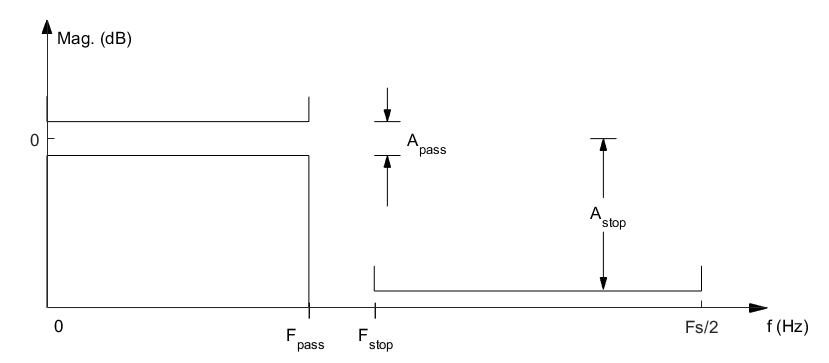
\includegraphics[width=0.8\textwidth]{figures/filter_req.png}
\caption{Requiremetns of a the lowpass filter.}
\label{fig:filter_req}
\end{figure}
From these the following conversion are made:
\begin{equation}
\omega_p=2\pi F_{pass}/Fs,\\
\omega_s=2\pi F_{stop}/Fs,\\
\delta_p=10^{A_{pass}/20},\\
\delta_s=10^{A_{stop}/20}
\end{equation}

To obtain a transfer function for a filter fulfilling the requirement the Kaiser window method is used.

\section{Kaiser Window Method}
The kaiser window method calculates the order of the filter and the beta value of the Kaiser window which is will be used to calculating the coefficients of the filter.

First the specification of the filter must be established: $\omega_p$, $\omega_s$, $\delta_p$ and $\delta_s$. For the kaiser window method the peak error $\delta$ will be the same in both the passband and stopband. which means: $\delta_p = \delta_s$ and the $\delta$ used is the lowest.

With the specifications established the cutoff frequency of the filter is found:
\begin{equation}
\omega_c=\frac{\omega_p+\omega_s}{2}
\end{equation}
Next the parameters for the Kaiser window must be determined:
\begin{equation}
\triangle\omega = \omega_s-\omega_p, \qquad\qquad A=-20log_{10}(\delta)
\end{equation}
The $\beta$ can the be calculated from:
\begin{equation} \label{eq:beta}
\beta=\left\{
\begin{array}{c l}      
    0,1102(A-8,7), & A>50,\\
    0,5842(A-21)^{0,4}+0,07886(A-21), & 21\leq A\leq 50\\
    0,0, & A<21.
\end{array}\right.
\end{equation}
and the order M can be calculated from:
\begin{equation}
M=\frac{A-8}{2,285\triangle\omega}
\end{equation}
Where M is predicted within $\pm$2. This leads to the calculation of the Kaiser window which is defined as:
\begin{equation} \label{eq:kaiserwindow}
w[n]=\left\{
\begin{array}{c l}      
    \frac{I_0[\beta(1-[n-\alpha)/\alpha]^2)^{1/2}]}{I_0(\beta)} & 0\leq n\leq M,\\
    0, & \textrm{otherwise},
\end{array}\right.
\end{equation}
Where $I_0$ is the zeroth-order modified Bessel function. The order of the FIR filter and the coefficients of the kaiser window can now be calculated and applied to the coefficients of the FIR filter which are derived below.

\subsection*{Implementation of FIR Filters}

The transfer function of a FIR filter is expressed as:
\begin{equation}
H(z) = \sum_{k=0}^{M} b_k z^{-k}
\end{equation}
The $b_k$ coefficients can be found by sampling the impulse response by M samples and afterwards applying a window function. The FIR only have zeros, thus cannot be unstable. To implement the filter the transfer function must be transformed into discrete time domain. First the transfer function is rewritten into following form:
\begin{equation}
H(z) = \frac{Y(z)}{X(z)} = \sum_{k=0}^{M} b_k z^{-k} \Leftrightarrow Y(z) = \sum_{k=0}^{M} b_k z^{-k} X(z) 
\end{equation}
The inverse z-transformation is applied which reveals:
\begin{equation}
y[n] = Z^{-1} \left\lbrace H(z)) \right\rbrace =\sum_{k=0}^{M} b_k x[n-k]
\end{equation}
The difference can now be implemented.



